\documentclass[twoside, 12pt]{article}

% Packages required by doxygen
\usepackage{calc, titleps, kantlipsum, doxygen, graphicx, makeidx, multirow}
\usepackage{multicol, textcomp, amssymb, sectsty, geometry, natbib}
\usepackage{amsmath, ifpdf, fancyhdr, caption, textcomp}
\usepackage[titles]{tocloft}
\PassOptionsToPackage{warn}{textcomp}
\usepackage[export]{adjustbox}
\usepackage[utf8]{inputenc}
\usepackage[nointegrals]{wasysym}
\usepackage[table]{xcolor}
\usepackage[pdftex,pagebackref=true]{hyperref}

% Font selection
\newcommand{\+}{\discretionary{\mbox{\scriptsize$\hookleftarrow$}}{}{}}
\newcommand{\project}{\textsc{Collaborate~}}
\newcommand{\cpp}{C\texttt{++}~}
\newcommand{\cppeleven}{C\texttt{++}11~}

% Page & text layout
\geometry{a4paper, top=3cm, bottom=1.75cm, left=1.75cm, right=1.75cm}
\widowpenalties 1 10000
\raggedbottom
\tolerance=0
\hfuzz=15pt
\hbadness=10000
\setlength{\emergencystretch}{15pt}
\setlength{\parindent}{0cm}
\setlength{\parskip}{3ex plus 2ex minus 2ex}
\makeatletter
\renewcommand{\paragraph}{
  \@startsection{paragraph}{4}{0ex}{-1.0ex}{1.0ex}{
    \normalfont\normalsize\bfseries\SS@parafont
  }
}
\renewcommand{\subparagraph}{
  \@startsection{subparagraph}{5}{0ex}{-1.0ex}{1.0ex}{
    \normalfont\normalsize\bfseries\SS@subparafont
  }
}
\makeatother

% Indices & bibliography
\setcounter{tocdepth}{2}
\setcounter{secnumdepth}{5}
\makeindex

% Hyperlinks (required, but should be loaded last)
\hypersetup{colorlinks=true, linkcolor=blue, citecolor=blue, unicode}

% Custom commands
\newcommand{\clearemptydoublepage}{
  \newpage{\pagestyle{empty}\cleardoublepage}
}

% Captions
\captionsetup{
  labelsep=space,
  justification=centering,
  font={bf},
  singlelinecheck=off,
  skip=4pt,position=top
}

%% -----------------------------------------------------------------------------

\begin{document}

\sloppy
\hypersetup{pageanchor=false, bookmarksnumbered=true, pdfencoding=unicode}

%% --- Title ---

\begin{titlepage}
\vspace*{5cm}
{\Huge\project} \\
\noindent\rule{\textwidth}{4pt}
Version 1.0
\hfill
July 6, 2019 \\
\mbox{}
\vfill
{\large ElectroScience Laboratory \hfill The Ohio State University} \\
\noindent\rule{\textwidth}{2pt}
\end{titlepage}

\pagenumbering{gobble}

%% --- License ---

\mbox{}
\vfill

Copyright (C) 2019  The Ohio State University

\project is free software, licensed under version 3 of the GNU Lesser General
Public License. See \texttt{https://www.gnu.org/licenses/} for details.

Sections of this document were assembled from comments in the source code using
Doxygen documentation tools.  All illustrations were created by the developers
using \project analysis software or associated software dependencies.

This research was sponsored by the NASA Advanced Information Systems Technology
Program \texttt{NNH16ZDA001N-AIST} and took place at the ElectroScience
Laboratory facility at The Ohio State University.

Permission is granted to copy, distribute and/or modify this document under the
terms of the GNU Free Documentation License, Version 1.3 or any later version
published by the Free Software Foundation; with no Invariant Sections, no
Front-Cover Texts, and no Back-Cover Texts.  A copy of the license is included
in the section entitled "GNU Free Documentation License".

\newpage

%% --- Table of Contents ---

\tableofcontents
\hypersetup{pageanchor=true}

\newpage

\pagestyle{fancy}
\renewcommand{\sectionmark}[1]{\markright{#1}{}}
\renewcommand{\headheight}{15pt}
\fancyhead[LO,RE]{\rightmark}
\fancyhead[LE,RO]{\thepage}
\cfoot{}

\pagenumbering{arabic}

\section{Python Script Execution}
\label{sec:orgdfb4f1e}
\subsection{Animate Data}
\label{sec:org06de043}
\begin{verbatim}
usage: animate_data.py [-h] [-f] [-i [IN_DIR]] [-o [OUT_DIR]] [-m [MONTH]]
                       [-v [VARIABLE]]

optional arguments:
  -h, --help            show this help message and exit
  -f, --figure          Whether to show or save
  -i [IN_DIR], --in_dir [IN_DIR]
                        Path to input directory
  -o [OUT_DIR], --out_dir [OUT_DIR]
                        Path to output directory
  -m [MONTH], --month [MONTH]
                        The month (2 digits)
  -v [VARIABLE], --variable [VARIABLE]
                        The netcdf variable name
\end{verbatim}

\subsection{Animate Map}
\label{sec:org143feb5}
\begin{verbatim}
usage: animate_map.py [-h] [-f] [-i [IN_FILE]] [-o [OUT_DIR]] [-d [DATA_DIR]]
                      [-t [TITLE]] [-w [WGT_PATH]] [-u [UWT_PATH]]

optional arguments:
  -h, --help            show this help message and exit
  -f, --figure          Whether to show or save
  -i [IN_FILE], --in_file [IN_FILE]
                        Path to input file
  -o [OUT_DIR], --out_dir [OUT_DIR]
                        Path to output directory
  -d [DATA_DIR], --data_dir [DATA_DIR]
                        Path to data directory
  -t [TITLE], --title [TITLE]
                        Title for the plot
  -w [WGT_PATH], --wgt_path [WGT_PATH]
                        Path to weighted adjacency list log
  -u [UWT_PATH], --uwt_path [UWT_PATH]
                        Path to unweighted adjacency list log
\end{verbatim}

\subsection{Animate Network}
\label{sec:orga73a9d6}
\begin{verbatim}
usage: animate_network.py [-h] [-f] [-i [IN_FILE]] [-o [OUT_FILE]] [-w]

optional arguments:
  -h, --help            show this help message and exit
  -f, --figure          Whether to show or save
  -i [IN_FILE], --in_file [IN_FILE]
                        Path to input file
  -o [OUT_FILE], --out_file [OUT_FILE]
                        Path to output directory
  -w, --weighted        Whether data is weighted
\end{verbatim}

\subsection{Plot Antenna}
\label{sec:org9863205}
\begin{verbatim}
usage: plot_antenna.py [-h] [-f] [-i [IN_FILE]] [-o [OUT_DIR]]

optional arguments:
  -h, --help            show this help message and exit
  -f, --figure          Whether to show or save
  -i [IN_FILE], --in_file [IN_FILE]
                        Path to input file
  -o [OUT_DIR], --out_dir [OUT_DIR]
                        Path to output directory
\end{verbatim}

\subsection{Plot Channel}
\label{sec:org4fa2a4c}
\begin{verbatim}
usage: plot_channel.py [-h] [-f] [-i [IN_DIR]] [-d [DATA_DIR]] [-o [OUT_DIR]]
                       [-n INDEX]

optional arguments:
  -h, --help            show this help message and exit
  -f, --figure          Whether to show or save
  -i [IN_DIR], --in_dir [IN_DIR]
                        Path to input directory
  -d [DATA_DIR], --data_dir [DATA_DIR]
                        Path to input directory
  -o [OUT_DIR], --out_dir [OUT_DIR]
                        Path to output directory
  -n INDEX, --index INDEX
                        The file index
\end{verbatim}

\subsection{Plot Data}
\label{sec:org7b15066}
\begin{verbatim}
usage: plot_data.py [-h] [-f] [-i [IN_DIR]] [-o [OUT_DIR]] [-n INDEX]
                    [-m [MONTH]] [-j [IN_DIR2]]

optional arguments:
  -h, --help            show this help message and exit
  -f, --figure          Whether to show or save
  -i [IN_DIR], --in_dir [IN_DIR]
                        Path to input directory
  -o [OUT_DIR], --out_dir [OUT_DIR]
                        Path to output directory
  -n INDEX, --index INDEX
                        The frame index
  -m [MONTH], --month [MONTH]
                        The month (2 digits)
  -j [IN_DIR2], --in_dir2 [IN_DIR2]
                        A second optional dataset
\end{verbatim}

\subsection{Plot Map}
\label{sec:org40aeaed}
\begin{verbatim}
usage: plot_map.py [-h] [-f] [-i [IN_FILE]] [-o [OUT_DIR]] [-n INDEX]
                   [-w [WGT_PATH]] [-u [UWT_PATH]]

optional arguments:
  -h, --help            show this help message and exit
  -f, --figure          Whether to show or save
  -i [IN_FILE], --in_file [IN_FILE]
                        Path to input file
  -o [OUT_DIR], --out_dir [OUT_DIR]
                        Path to output directory
  -n INDEX, --index INDEX
                        The frame index
  -w [WGT_PATH], --wgt_path [WGT_PATH]
                        Path to weighted adjacency list log
  -u [UWT_PATH], --uwt_path [UWT_PATH]
                        Path to unweighted adjacency list log
\end{verbatim}

\subsection{Plot Measurement}
\label{sec:org1737f2f}
\begin{verbatim}
usage: plot_measurement.py [-h] [-i [IN_DIR]] [-d [DATA_DIR]] [-o [OUT_DIR]]
                           [-n INDEX]

optional arguments:
  -h, --help            show this help message and exit
  -i [IN_DIR], --in_dir [IN_DIR]
                        Path to input directory
  -d [DATA_DIR], --data_dir [DATA_DIR]
                        Path to input directory
  -o [OUT_DIR], --out_dir [OUT_DIR]
                        Path to output directory
  -n INDEX, --index INDEX
                        The file index
\end{verbatim}

\subsection{Plot Network}
\label{sec:org037bf1f}
\begin{verbatim}
usage: plot_network.py [-h] [-i [IN_FILE]] [-o [OUT_DIR]] [-n INDEX] [-w] [-f]

optional arguments:
  -h, --help            show this help message and exit
  -i [IN_FILE], --in_file [IN_FILE]
                        Path to input file
  -o [OUT_DIR], --out_dir [OUT_DIR]
                        Path to output directory
  -n INDEX, --index INDEX
                        The frame index
  -w, --weighted        Whether data is weighted
  -f, --figure          Whether to show or save
\end{verbatim}

\subsection{Plot Series}
\label{sec:orgd690f64}
\begin{verbatim}
usage: plot_series.py [-h] [-i [IN_FILE]] [-o [OUT_DIR]] [-n INDEX] [-f]

optional arguments:
  -h, --help            show this help message and exit
  -i [IN_FILE], --in_file [IN_FILE]
                        Path to input file
  -o [OUT_DIR], --out_dir [OUT_DIR]
                        Path to output directory
  -n INDEX, --index INDEX
                        The frame index
  -f, --figure          Whether to show or save
\end{verbatim}


%% --- Data Structures ---

\section{\cpp Classes}
\hypertarget{classosse_1_1collaborate_1_1_antenna_dipole}{}\subsection{osse\+:\+:collaborate\+:\+:Antenna\+Dipole Class Reference}
\label{classosse_1_1collaborate_1_1_antenna_dipole}\index{osse\+::collaborate\+::\+Antenna\+Dipole@{osse\+::collaborate\+::\+Antenna\+Dipole}}


An approximation of a dipole antenna.  




{\ttfamily \#include $<$antenna\+\_\+dipole.\+h$>$}



Inheritance diagram for osse\+:\+:collaborate\+:\+:Antenna\+Dipole\+:
\nopagebreak
\begin{figure}[H]
\begin{center}
\leavevmode
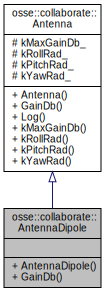
\includegraphics[width=187pt]{classosse_1_1collaborate_1_1_antenna_dipole__inherit__graph}
\end{center}
\end{figure}
\subsubsection*{Public Member Functions}
\begin{DoxyCompactItemize}
\item 
\hyperlink{classosse_1_1collaborate_1_1_antenna_dipole_ab3146ec94f0d032743c5277d1f56b3d2}{Antenna\+Dipole} (const double \&\+\_\+max\+\_\+gain\+\_\+db, const double \&\+\_\+roll\+\_\+rad, const double \&\+\_\+pitch\+\_\+rad, const double \&\+\_\+yaw\+\_\+rad)
\begin{DoxyCompactList}\small\item\em Constructor. \end{DoxyCompactList}\item 
double \hyperlink{classosse_1_1collaborate_1_1_antenna_dipole_a46aab376eb3bb44ae47beceef79db8df}{Gain\+Db} (const double \&\+\_\+theta\+\_\+rad, const double \&\+\_\+phi\+\_\+rad) const
\begin{DoxyCompactList}\small\item\em Obtain directional gain (decibels) \end{DoxyCompactList}\end{DoxyCompactItemize}
\subsubsection*{Additional Inherited Members}


\subsubsection{Detailed Description}
An approximation of a dipole antenna. 

 
\begin{DoxyImageNoCaption}
  \mbox{\includegraphics[width=0.5\textwidth]{dipole}}
\end{DoxyImageNoCaption}


\[ g = g_{max}\sin^2{\theta}~~~(decibels) \] 

\subsubsection{Constructor \& Destructor Documentation}
\mbox{\Hypertarget{classosse_1_1collaborate_1_1_antenna_dipole_ab3146ec94f0d032743c5277d1f56b3d2}\label{classosse_1_1collaborate_1_1_antenna_dipole_ab3146ec94f0d032743c5277d1f56b3d2}} 
\index{osse\+::collaborate\+::\+Antenna\+Dipole@{osse\+::collaborate\+::\+Antenna\+Dipole}!Antenna\+Dipole@{Antenna\+Dipole}}
\index{Antenna\+Dipole@{Antenna\+Dipole}!osse\+::collaborate\+::\+Antenna\+Dipole@{osse\+::collaborate\+::\+Antenna\+Dipole}}
\paragraph{\texorpdfstring{Antenna\+Dipole()}{AntennaDipole()}}
{\footnotesize\ttfamily osse\+::collaborate\+::\+Antenna\+Dipole\+::\+Antenna\+Dipole (\begin{DoxyParamCaption}\item[{const double \&}]{\+\_\+max\+\_\+gain\+\_\+db,  }\item[{const double \&}]{\+\_\+roll\+\_\+rad,  }\item[{const double \&}]{\+\_\+pitch\+\_\+rad,  }\item[{const double \&}]{\+\_\+yaw\+\_\+rad }\end{DoxyParamCaption})}



Constructor. 


\begin{DoxyParams}[1]{Parameters}
\mbox{\tt in}  & {\em \+\_\+max\+\_\+gain\+\_\+db} & The maximum gain (decibels) \\
\hline
\mbox{\tt in}  & {\em \+\_\+roll\+\_\+rad} & Roll angle to host body frame (radians) \\
\hline
\mbox{\tt in}  & {\em \+\_\+pitch\+\_\+rad} & Pitch angle to host body frame (radians) \\
\hline
\mbox{\tt in}  & {\em \+\_\+yaw\+\_\+rad} & Yaw angle to host body frame (radians) \\
\hline
\end{DoxyParams}


\subsubsection{Member Function Documentation}
\mbox{\Hypertarget{classosse_1_1collaborate_1_1_antenna_dipole_a46aab376eb3bb44ae47beceef79db8df}\label{classosse_1_1collaborate_1_1_antenna_dipole_a46aab376eb3bb44ae47beceef79db8df}} 
\index{osse\+::collaborate\+::\+Antenna\+Dipole@{osse\+::collaborate\+::\+Antenna\+Dipole}!Gain\+Db@{Gain\+Db}}
\index{Gain\+Db@{Gain\+Db}!osse\+::collaborate\+::\+Antenna\+Dipole@{osse\+::collaborate\+::\+Antenna\+Dipole}}
\paragraph{\texorpdfstring{Gain\+Db()}{GainDb()}}
{\footnotesize\ttfamily double osse\+::collaborate\+::\+Antenna\+Dipole\+::\+Gain\+Db (\begin{DoxyParamCaption}\item[{const double \&}]{\+\_\+theta\+\_\+rad,  }\item[{const double \&}]{\+\_\+phi\+\_\+rad }\end{DoxyParamCaption}) const\hspace{0.3cm}{\ttfamily [virtual]}}



Obtain directional gain (decibels) 


\begin{DoxyParams}[1]{Parameters}
\mbox{\tt in}  & {\em \+\_\+theta\+\_\+rad} & Altitude angle from positive z-\/axis (radians) \\
\hline
\mbox{\tt in}  & {\em \+\_\+phi\+\_\+rad} & Azimuth angle (radians) \\
\hline
\end{DoxyParams}
\begin{DoxyReturn}{Returns}
Directional gain (decibels)
\end{DoxyReturn}
\[ g = g_{max}\sin^2{\theta}~~~(decibels) \] 

Implements \hyperlink{classosse_1_1collaborate_1_1_antenna_a67214b4b28f3d48931c8fb435cc1f85d}{osse\+::collaborate\+::\+Antenna}.



The documentation for this class was generated from the following files\+:\begin{DoxyCompactItemize}
\item 
libs/collaborate/include/collaborate/antenna\+\_\+dipole.\+h\item 
libs/collaborate/src/antenna\+\_\+dipole.\+cpp\end{DoxyCompactItemize}

\hypertarget{classosse_1_1collaborate_1_1_antenna_helical}{}\subsection{osse\+:\+:collaborate\+:\+:Antenna\+Helical Class Reference}
\label{classosse_1_1collaborate_1_1_antenna_helical}\index{osse\+::collaborate\+::\+Antenna\+Helical@{osse\+::collaborate\+::\+Antenna\+Helical}}


An approximation of a helical antenna (more directional than patch)  




{\ttfamily \#include $<$antenna\+\_\+helical.\+h$>$}



Inheritance diagram for osse\+:\+:collaborate\+:\+:Antenna\+Helical\+:
\nopagebreak
\begin{figure}[H]
\begin{center}
\leavevmode
\includegraphics[width=190pt]{classosse_1_1collaborate_1_1_antenna_helical__inherit__graph}
\end{center}
\end{figure}
\subsubsection*{Public Member Functions}
\begin{DoxyCompactItemize}
\item 
\hyperlink{classosse_1_1collaborate_1_1_antenna_helical_a2984fb54d37462763ca923c0ba5d4893}{Antenna\+Helical} (const double \&\+\_\+max\+\_\+gain\+\_\+db, const double \&\+\_\+roll\+\_\+rad, const double \&\+\_\+pitch\+\_\+rad, const double \&\+\_\+yaw\+\_\+rad)
\begin{DoxyCompactList}\small\item\em Constructor. \end{DoxyCompactList}\item 
double \hyperlink{classosse_1_1collaborate_1_1_antenna_helical_ac405a2e34ec76610b88d8f1fb407658d}{Gain\+Db} (const double \&\+\_\+theta\+\_\+rad, const double \&\+\_\+phi\+\_\+rad) const
\begin{DoxyCompactList}\small\item\em Obtain directional gain (decibels) \end{DoxyCompactList}\end{DoxyCompactItemize}
\subsubsection*{Additional Inherited Members}


\subsubsection{Detailed Description}
An approximation of a helical antenna (more directional than patch) 

 
\begin{DoxyImageNoCaption}
  \mbox{\includegraphics[width=0.5\textwidth]{helical}}
\end{DoxyImageNoCaption}


\[ g = g_{max}\cos^{50}{\theta}~~~(decibels) \] 

\subsubsection{Constructor \& Destructor Documentation}
\mbox{\Hypertarget{classosse_1_1collaborate_1_1_antenna_helical_a2984fb54d37462763ca923c0ba5d4893}\label{classosse_1_1collaborate_1_1_antenna_helical_a2984fb54d37462763ca923c0ba5d4893}} 
\index{osse\+::collaborate\+::\+Antenna\+Helical@{osse\+::collaborate\+::\+Antenna\+Helical}!Antenna\+Helical@{Antenna\+Helical}}
\index{Antenna\+Helical@{Antenna\+Helical}!osse\+::collaborate\+::\+Antenna\+Helical@{osse\+::collaborate\+::\+Antenna\+Helical}}
\paragraph{\texorpdfstring{Antenna\+Helical()}{AntennaHelical()}}
{\footnotesize\ttfamily osse\+::collaborate\+::\+Antenna\+Helical\+::\+Antenna\+Helical (\begin{DoxyParamCaption}\item[{const double \&}]{\+\_\+max\+\_\+gain\+\_\+db,  }\item[{const double \&}]{\+\_\+roll\+\_\+rad,  }\item[{const double \&}]{\+\_\+pitch\+\_\+rad,  }\item[{const double \&}]{\+\_\+yaw\+\_\+rad }\end{DoxyParamCaption})}



Constructor. 


\begin{DoxyParams}[1]{Parameters}
\mbox{\tt in}  & {\em \+\_\+max\+\_\+gain\+\_\+db} & Maximum gain (decibels) \\
\hline
\mbox{\tt in}  & {\em \+\_\+roll\+\_\+rad} & Roll angle to host body reference frame (radians) \\
\hline
\mbox{\tt in}  & {\em \+\_\+pitch\+\_\+rad} & Pitch angle to host body reference frame (radians) \\
\hline
\mbox{\tt in}  & {\em \+\_\+yaw\+\_\+rad} & Yaw angle to host body reference frame (radians) \\
\hline
\end{DoxyParams}


\subsubsection{Member Function Documentation}
\mbox{\Hypertarget{classosse_1_1collaborate_1_1_antenna_helical_ac405a2e34ec76610b88d8f1fb407658d}\label{classosse_1_1collaborate_1_1_antenna_helical_ac405a2e34ec76610b88d8f1fb407658d}} 
\index{osse\+::collaborate\+::\+Antenna\+Helical@{osse\+::collaborate\+::\+Antenna\+Helical}!Gain\+Db@{Gain\+Db}}
\index{Gain\+Db@{Gain\+Db}!osse\+::collaborate\+::\+Antenna\+Helical@{osse\+::collaborate\+::\+Antenna\+Helical}}
\paragraph{\texorpdfstring{Gain\+Db()}{GainDb()}}
{\footnotesize\ttfamily double osse\+::collaborate\+::\+Antenna\+Helical\+::\+Gain\+Db (\begin{DoxyParamCaption}\item[{const double \&}]{\+\_\+theta\+\_\+rad,  }\item[{const double \&}]{\+\_\+phi\+\_\+rad }\end{DoxyParamCaption}) const\hspace{0.3cm}{\ttfamily [virtual]}}



Obtain directional gain (decibels) 


\begin{DoxyParams}[1]{Parameters}
\mbox{\tt in}  & {\em \+\_\+theta\+\_\+rad} & Altitude angle from positive z-\/axis (radians) \\
\hline
\mbox{\tt in}  & {\em \+\_\+phi\+\_\+rad} & Azimuth angle (radians) \\
\hline
\end{DoxyParams}
\begin{DoxyReturn}{Returns}
Directional gain (decibels)
\end{DoxyReturn}
\[ g = g_{max}\cos^{50}{\theta}~~~(decibels) \] 

Implements \hyperlink{classosse_1_1collaborate_1_1_antenna_a67214b4b28f3d48931c8fb435cc1f85d}{osse\+::collaborate\+::\+Antenna}.



The documentation for this class was generated from the following files\+:\begin{DoxyCompactItemize}
\item 
libs/collaborate/include/collaborate/antenna\+\_\+helical.\+h\item 
libs/collaborate/src/antenna\+\_\+helical.\+cpp\end{DoxyCompactItemize}

\hypertarget{classosse_1_1collaborate_1_1_antenna_isotropic}{}\subsection{osse\+:\+:collaborate\+:\+:Antenna\+Isotropic Class Reference}
\label{classosse_1_1collaborate_1_1_antenna_isotropic}\index{osse\+::collaborate\+::\+Antenna\+Isotropic@{osse\+::collaborate\+::\+Antenna\+Isotropic}}


An isotropic antenna.  




{\ttfamily \#include $<$antenna\+\_\+isotropic.\+h$>$}



Inheritance diagram for osse\+:\+:collaborate\+:\+:Antenna\+Isotropic\+:
\nopagebreak
\begin{figure}[H]
\begin{center}
\leavevmode
\includegraphics[width=198pt]{classosse_1_1collaborate_1_1_antenna_isotropic__inherit__graph}
\end{center}
\end{figure}
\subsubsection*{Public Member Functions}
\begin{DoxyCompactItemize}
\item 
\hyperlink{classosse_1_1collaborate_1_1_antenna_isotropic_ae431744ad97d6b0a1d25039e94b4ffcb}{Antenna\+Isotropic} (const double \&\+\_\+max\+\_\+gain\+\_\+db)
\begin{DoxyCompactList}\small\item\em Constructor. \end{DoxyCompactList}\item 
double \hyperlink{classosse_1_1collaborate_1_1_antenna_isotropic_ab695187eb238b78ac03f27bd1cbffc11}{Gain\+Db} (const double \&\+\_\+theta\+\_\+rad, const double \&\+\_\+phi\+\_\+rad) const
\begin{DoxyCompactList}\small\item\em Obtain directional gain (decibels) \end{DoxyCompactList}\end{DoxyCompactItemize}
\subsubsection*{Additional Inherited Members}


\subsubsection{Detailed Description}
An isotropic antenna. 

 
\begin{DoxyImageNoCaption}
  \mbox{\includegraphics[width=0.5\textwidth]{isotropic}}
\end{DoxyImageNoCaption}


\[ g = g_{max}~~~(decibels) \] 

\subsubsection{Constructor \& Destructor Documentation}
\mbox{\Hypertarget{classosse_1_1collaborate_1_1_antenna_isotropic_ae431744ad97d6b0a1d25039e94b4ffcb}\label{classosse_1_1collaborate_1_1_antenna_isotropic_ae431744ad97d6b0a1d25039e94b4ffcb}} 
\index{osse\+::collaborate\+::\+Antenna\+Isotropic@{osse\+::collaborate\+::\+Antenna\+Isotropic}!Antenna\+Isotropic@{Antenna\+Isotropic}}
\index{Antenna\+Isotropic@{Antenna\+Isotropic}!osse\+::collaborate\+::\+Antenna\+Isotropic@{osse\+::collaborate\+::\+Antenna\+Isotropic}}
\paragraph{\texorpdfstring{Antenna\+Isotropic()}{AntennaIsotropic()}}
{\footnotesize\ttfamily osse\+::collaborate\+::\+Antenna\+Isotropic\+::\+Antenna\+Isotropic (\begin{DoxyParamCaption}\item[{const double \&}]{\+\_\+max\+\_\+gain\+\_\+db }\end{DoxyParamCaption})\hspace{0.3cm}{\ttfamily [explicit]}}



Constructor. 


\begin{DoxyParams}[1]{Parameters}
\mbox{\tt in}  & {\em \+\_\+max\+\_\+gain\+\_\+db} & Maximum gain (decibels) \\
\hline
\end{DoxyParams}


\subsubsection{Member Function Documentation}
\mbox{\Hypertarget{classosse_1_1collaborate_1_1_antenna_isotropic_ab695187eb238b78ac03f27bd1cbffc11}\label{classosse_1_1collaborate_1_1_antenna_isotropic_ab695187eb238b78ac03f27bd1cbffc11}} 
\index{osse\+::collaborate\+::\+Antenna\+Isotropic@{osse\+::collaborate\+::\+Antenna\+Isotropic}!Gain\+Db@{Gain\+Db}}
\index{Gain\+Db@{Gain\+Db}!osse\+::collaborate\+::\+Antenna\+Isotropic@{osse\+::collaborate\+::\+Antenna\+Isotropic}}
\paragraph{\texorpdfstring{Gain\+Db()}{GainDb()}}
{\footnotesize\ttfamily double osse\+::collaborate\+::\+Antenna\+Isotropic\+::\+Gain\+Db (\begin{DoxyParamCaption}\item[{const double \&}]{\+\_\+theta\+\_\+rad,  }\item[{const double \&}]{\+\_\+phi\+\_\+rad }\end{DoxyParamCaption}) const\hspace{0.3cm}{\ttfamily [virtual]}}



Obtain directional gain (decibels) 


\begin{DoxyParams}[1]{Parameters}
\mbox{\tt in}  & {\em \+\_\+theta\+\_\+rad} & Altitude angle from positive z-\/axis (radians) \\
\hline
\mbox{\tt in}  & {\em \+\_\+phi\+\_\+rad} & Azimuth angle (radians) \\
\hline
\end{DoxyParams}
\begin{DoxyReturn}{Returns}
Directional gain (decibels)
\end{DoxyReturn}
\[ g = g_{max}~~~(decibels) \] 

Implements \hyperlink{classosse_1_1collaborate_1_1_antenna_a67214b4b28f3d48931c8fb435cc1f85d}{osse\+::collaborate\+::\+Antenna}.



The documentation for this class was generated from the following files\+:\begin{DoxyCompactItemize}
\item 
libs/collaborate/include/collaborate/antenna\+\_\+isotropic.\+h\item 
libs/collaborate/src/antenna\+\_\+isotropic.\+cpp\end{DoxyCompactItemize}

\hypertarget{classosse_1_1collaborate_1_1_antenna_patch}{}\subsection{osse\+:\+:collaborate\+:\+:Antenna\+Patch Class Reference}
\label{classosse_1_1collaborate_1_1_antenna_patch}\index{osse\+::collaborate\+::\+Antenna\+Patch@{osse\+::collaborate\+::\+Antenna\+Patch}}


An approximation of a patch antenna.  




{\ttfamily \#include $<$antenna\+\_\+patch.\+h$>$}



Inheritance diagram for osse\+:\+:collaborate\+:\+:Antenna\+Patch\+:
\nopagebreak
\begin{figure}[H]
\begin{center}
\leavevmode
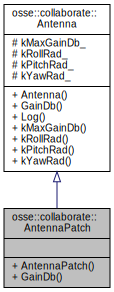
\includegraphics[width=186pt]{classosse_1_1collaborate_1_1_antenna_patch__inherit__graph}
\end{center}
\end{figure}
\subsubsection*{Public Member Functions}
\begin{DoxyCompactItemize}
\item 
\hyperlink{classosse_1_1collaborate_1_1_antenna_patch_a317eea4be3b7de724dd8a3d3f83a975f}{Antenna\+Patch} (const double \&\+\_\+max\+\_\+gain\+\_\+db, const double \&\+\_\+roll\+\_\+rad, const double \&\+\_\+pitch\+\_\+rad, const double \&\+\_\+yaw\+\_\+rad)
\begin{DoxyCompactList}\small\item\em Constructor. \end{DoxyCompactList}\item 
double \hyperlink{classosse_1_1collaborate_1_1_antenna_patch_a34cd1ff37a5851f9dab72d737f72d0de}{Gain\+Db} (const double \&\+\_\+theta\+\_\+rad, const double \&\+\_\+phi\+\_\+rad) const
\begin{DoxyCompactList}\small\item\em Obtain directional gain (decibels) \end{DoxyCompactList}\end{DoxyCompactItemize}
\subsubsection*{Additional Inherited Members}


\subsubsection{Detailed Description}
An approximation of a patch antenna. 

 
\begin{DoxyImageNoCaption}
  \mbox{\includegraphics[width=0.5\textwidth]{patch}}
\end{DoxyImageNoCaption}


\[ g = g_{max}\cos{\theta}~~~(decibels),~~~~~0<\theta\le\pi/2 \] 

\subsubsection{Constructor \& Destructor Documentation}
\mbox{\Hypertarget{classosse_1_1collaborate_1_1_antenna_patch_a317eea4be3b7de724dd8a3d3f83a975f}\label{classosse_1_1collaborate_1_1_antenna_patch_a317eea4be3b7de724dd8a3d3f83a975f}} 
\index{osse\+::collaborate\+::\+Antenna\+Patch@{osse\+::collaborate\+::\+Antenna\+Patch}!Antenna\+Patch@{Antenna\+Patch}}
\index{Antenna\+Patch@{Antenna\+Patch}!osse\+::collaborate\+::\+Antenna\+Patch@{osse\+::collaborate\+::\+Antenna\+Patch}}
\paragraph{\texorpdfstring{Antenna\+Patch()}{AntennaPatch()}}
{\footnotesize\ttfamily osse\+::collaborate\+::\+Antenna\+Patch\+::\+Antenna\+Patch (\begin{DoxyParamCaption}\item[{const double \&}]{\+\_\+max\+\_\+gain\+\_\+db,  }\item[{const double \&}]{\+\_\+roll\+\_\+rad,  }\item[{const double \&}]{\+\_\+pitch\+\_\+rad,  }\item[{const double \&}]{\+\_\+yaw\+\_\+rad }\end{DoxyParamCaption})}



Constructor. 


\begin{DoxyParams}[1]{Parameters}
\mbox{\tt in}  & {\em \+\_\+max\+\_\+gain\+\_\+db} & Maximum gain (decibels) \\
\hline
\mbox{\tt in}  & {\em \+\_\+roll\+\_\+rad} & Roll angle to host body reference frame (radians) \\
\hline
\mbox{\tt in}  & {\em \+\_\+pitch\+\_\+rad} & Pitch angle to host body reference frame (radians) \\
\hline
\mbox{\tt in}  & {\em \+\_\+yaw\+\_\+rad} & Yaw angle to host body reference frame (radians) \\
\hline
\end{DoxyParams}


\subsubsection{Member Function Documentation}
\mbox{\Hypertarget{classosse_1_1collaborate_1_1_antenna_patch_a34cd1ff37a5851f9dab72d737f72d0de}\label{classosse_1_1collaborate_1_1_antenna_patch_a34cd1ff37a5851f9dab72d737f72d0de}} 
\index{osse\+::collaborate\+::\+Antenna\+Patch@{osse\+::collaborate\+::\+Antenna\+Patch}!Gain\+Db@{Gain\+Db}}
\index{Gain\+Db@{Gain\+Db}!osse\+::collaborate\+::\+Antenna\+Patch@{osse\+::collaborate\+::\+Antenna\+Patch}}
\paragraph{\texorpdfstring{Gain\+Db()}{GainDb()}}
{\footnotesize\ttfamily double osse\+::collaborate\+::\+Antenna\+Patch\+::\+Gain\+Db (\begin{DoxyParamCaption}\item[{const double \&}]{\+\_\+theta\+\_\+rad,  }\item[{const double \&}]{\+\_\+phi\+\_\+rad }\end{DoxyParamCaption}) const\hspace{0.3cm}{\ttfamily [virtual]}}



Obtain directional gain (decibels) 


\begin{DoxyParams}[1]{Parameters}
\mbox{\tt in}  & {\em \+\_\+theta\+\_\+rad} & Altitude angle from positive z-\/axis (radians) \\
\hline
\mbox{\tt in}  & {\em \+\_\+phi\+\_\+rad} & Azimuth angle (radians) \\
\hline
\end{DoxyParams}
\begin{DoxyReturn}{Returns}
Directional gain (decibels)
\end{DoxyReturn}
\[ g = g_{max}\cos{\theta}~~~(decibels),~~~~~0<\theta\le\pi/2 \] 

Implements \hyperlink{classosse_1_1collaborate_1_1_antenna_a67214b4b28f3d48931c8fb435cc1f85d}{osse\+::collaborate\+::\+Antenna}.



The documentation for this class was generated from the following files\+:\begin{DoxyCompactItemize}
\item 
libs/collaborate/include/collaborate/antenna\+\_\+patch.\+h\item 
libs/collaborate/src/antenna\+\_\+patch.\+cpp\end{DoxyCompactItemize}

\hypertarget{classosse_1_1collaborate_1_1_antenna}{}\subsection{osse\+:\+:collaborate\+:\+:Antenna Class Reference}
\label{classosse_1_1collaborate_1_1_antenna}\index{osse\+::collaborate\+::\+Antenna@{osse\+::collaborate\+::\+Antenna}}


Abstract antenna.  




{\ttfamily \#include $<$antenna.\+h$>$}



Inheritance diagram for osse\+:\+:collaborate\+:\+:Antenna\+:
\nopagebreak
\begin{figure}[H]
\begin{center}
\leavevmode
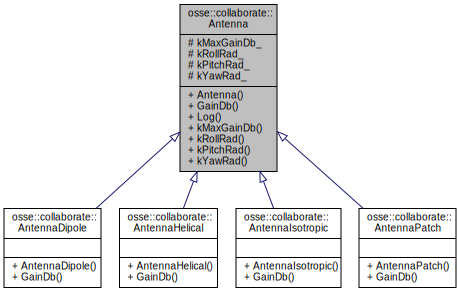
\includegraphics[width=350pt]{classosse_1_1collaborate_1_1_antenna__inherit__graph}
\end{center}
\end{figure}
\subsubsection*{Public Member Functions}
\begin{DoxyCompactItemize}
\item 
\hyperlink{classosse_1_1collaborate_1_1_antenna_a0f871800c6102bc92a2bda159f43b240}{Antenna} (const double \&\+\_\+max\+\_\+gain\+\_\+db, const double \&\+\_\+roll\+\_\+rad, const double \&\+\_\+pitch\+\_\+rad, const double \&\+\_\+yaw\+\_\+rad)
\begin{DoxyCompactList}\small\item\em Constructor. \end{DoxyCompactList}\item 
virtual double \hyperlink{classosse_1_1collaborate_1_1_antenna_a67214b4b28f3d48931c8fb435cc1f85d}{Gain\+Db} (const double \&\+\_\+theta\+\_\+rad, const double \&\+\_\+phi\+\_\+rad) const =0
\begin{DoxyCompactList}\small\item\em Obtain directional gain (decibels) \end{DoxyCompactList}\item 
void \hyperlink{classosse_1_1collaborate_1_1_antenna_ae24d52fa84fd3acff597c56259f4aba6}{Log} (const std\+::string \&\+\_\+path) const
\begin{DoxyCompactList}\small\item\em Logs the antenna pattern to a file. \end{DoxyCompactList}\item 
const double \& \hyperlink{classosse_1_1collaborate_1_1_antenna_a0666d28c6d44c193d4abd844a04044b4}{k\+Max\+Gain\+Db} () const
\begin{DoxyCompactList}\small\item\em Get maximum gain (decibels) \end{DoxyCompactList}\item 
const double \& \hyperlink{classosse_1_1collaborate_1_1_antenna_ac6602825c2e7282bc89f01b45f3289b7}{k\+Roll\+Rad} () const
\begin{DoxyCompactList}\small\item\em Get roll angle to host body reference frame (radians) \end{DoxyCompactList}\item 
const double \& \hyperlink{classosse_1_1collaborate_1_1_antenna_a3216890f8adcd7f52bbf9af7fef2f45f}{k\+Pitch\+Rad} () const
\begin{DoxyCompactList}\small\item\em Get pitch angle to host body reference frame (radians) \end{DoxyCompactList}\item 
const double \& \hyperlink{classosse_1_1collaborate_1_1_antenna_a79acbd84d9ad9a739ec0a8c60b49bc93}{k\+Yaw\+Rad} () const
\begin{DoxyCompactList}\small\item\em Get yaw angle to host body reference frame (radians) \end{DoxyCompactList}\end{DoxyCompactItemize}
\subsubsection*{Protected Attributes}
\begin{DoxyCompactItemize}
\item 
\mbox{\Hypertarget{classosse_1_1collaborate_1_1_antenna_a3bb8d000dfd0dbd4713cc1c4fbc8772e}\label{classosse_1_1collaborate_1_1_antenna_a3bb8d000dfd0dbd4713cc1c4fbc8772e}} 
const double \hyperlink{classosse_1_1collaborate_1_1_antenna_a3bb8d000dfd0dbd4713cc1c4fbc8772e}{k\+Max\+Gain\+Db\+\_\+}
\begin{DoxyCompactList}\small\item\em Maximum gain (decibels) \end{DoxyCompactList}\item 
\mbox{\Hypertarget{classosse_1_1collaborate_1_1_antenna_aff899094f1534787d2ce4899a6d1babb}\label{classosse_1_1collaborate_1_1_antenna_aff899094f1534787d2ce4899a6d1babb}} 
const double \hyperlink{classosse_1_1collaborate_1_1_antenna_aff899094f1534787d2ce4899a6d1babb}{k\+Roll\+Rad\+\_\+}
\begin{DoxyCompactList}\small\item\em Roll angle to host body reference frame (radians) \end{DoxyCompactList}\item 
\mbox{\Hypertarget{classosse_1_1collaborate_1_1_antenna_a05c6fd112ee735a371ed48f0a9b3701f}\label{classosse_1_1collaborate_1_1_antenna_a05c6fd112ee735a371ed48f0a9b3701f}} 
const double \hyperlink{classosse_1_1collaborate_1_1_antenna_a05c6fd112ee735a371ed48f0a9b3701f}{k\+Pitch\+Rad\+\_\+}
\begin{DoxyCompactList}\small\item\em Pitch angle to host body reference frame (radians) \end{DoxyCompactList}\item 
\mbox{\Hypertarget{classosse_1_1collaborate_1_1_antenna_abb5b0f5a06d029eba6029f143588c99b}\label{classosse_1_1collaborate_1_1_antenna_abb5b0f5a06d029eba6029f143588c99b}} 
const double \hyperlink{classosse_1_1collaborate_1_1_antenna_abb5b0f5a06d029eba6029f143588c99b}{k\+Yaw\+Rad\+\_\+}
\begin{DoxyCompactList}\small\item\em Yaw angle to host body reference frame (radians) \end{DoxyCompactList}\end{DoxyCompactItemize}


\subsubsection{Detailed Description}
Abstract antenna. 

 
\begin{DoxyImageNoCaption}
  \mbox{\includegraphics[width=\textwidth]{antennas}}
\end{DoxyImageNoCaption}
 

\subsubsection{Constructor \& Destructor Documentation}
\mbox{\Hypertarget{classosse_1_1collaborate_1_1_antenna_a0f871800c6102bc92a2bda159f43b240}\label{classosse_1_1collaborate_1_1_antenna_a0f871800c6102bc92a2bda159f43b240}} 
\index{osse\+::collaborate\+::\+Antenna@{osse\+::collaborate\+::\+Antenna}!Antenna@{Antenna}}
\index{Antenna@{Antenna}!osse\+::collaborate\+::\+Antenna@{osse\+::collaborate\+::\+Antenna}}
\paragraph{\texorpdfstring{Antenna()}{Antenna()}}
{\footnotesize\ttfamily osse\+::collaborate\+::\+Antenna\+::\+Antenna (\begin{DoxyParamCaption}\item[{const double \&}]{\+\_\+max\+\_\+gain\+\_\+db,  }\item[{const double \&}]{\+\_\+roll\+\_\+rad,  }\item[{const double \&}]{\+\_\+pitch\+\_\+rad,  }\item[{const double \&}]{\+\_\+yaw\+\_\+rad }\end{DoxyParamCaption})}



Constructor. 


\begin{DoxyParams}[1]{Parameters}
\mbox{\tt in}  & {\em \+\_\+max\+\_\+gain\+\_\+db} & Maximum gain (decibels) \\
\hline
\mbox{\tt in}  & {\em \+\_\+roll\+\_\+rad} & Roll angle to host body reference frame (radians) \\
\hline
\mbox{\tt in}  & {\em \+\_\+pitch\+\_\+rad} & Pitch angle to host body reference frame (radians) \\
\hline
\mbox{\tt in}  & {\em \+\_\+yaw\+\_\+rad} & Yaw angle to host body reference frame (radians) \\
\hline
\end{DoxyParams}


\subsubsection{Member Function Documentation}
\mbox{\Hypertarget{classosse_1_1collaborate_1_1_antenna_a67214b4b28f3d48931c8fb435cc1f85d}\label{classosse_1_1collaborate_1_1_antenna_a67214b4b28f3d48931c8fb435cc1f85d}} 
\index{osse\+::collaborate\+::\+Antenna@{osse\+::collaborate\+::\+Antenna}!Gain\+Db@{Gain\+Db}}
\index{Gain\+Db@{Gain\+Db}!osse\+::collaborate\+::\+Antenna@{osse\+::collaborate\+::\+Antenna}}
\paragraph{\texorpdfstring{Gain\+Db()}{GainDb()}}
{\footnotesize\ttfamily virtual double osse\+::collaborate\+::\+Antenna\+::\+Gain\+Db (\begin{DoxyParamCaption}\item[{const double \&}]{\+\_\+theta\+\_\+rad,  }\item[{const double \&}]{\+\_\+phi\+\_\+rad }\end{DoxyParamCaption}) const\hspace{0.3cm}{\ttfamily [pure virtual]}}



Obtain directional gain (decibels) 


\begin{DoxyParams}[1]{Parameters}
\mbox{\tt in}  & {\em \+\_\+theta\+\_\+rad} & Altitude angle from positive z-\/axis (radians) \\
\hline
\mbox{\tt in}  & {\em \+\_\+phi\+\_\+rad} & Azimuth angle (radians) \\
\hline
\end{DoxyParams}
\begin{DoxyReturn}{Returns}
Directional gain (decibels) 
\end{DoxyReturn}


Implemented in \hyperlink{classosse_1_1collaborate_1_1_antenna_dipole_a46aab376eb3bb44ae47beceef79db8df}{osse\+::collaborate\+::\+Antenna\+Dipole}, \hyperlink{classosse_1_1collaborate_1_1_antenna_helical_ac405a2e34ec76610b88d8f1fb407658d}{osse\+::collaborate\+::\+Antenna\+Helical}, \hyperlink{classosse_1_1collaborate_1_1_antenna_patch_a34cd1ff37a5851f9dab72d737f72d0de}{osse\+::collaborate\+::\+Antenna\+Patch}, and \hyperlink{classosse_1_1collaborate_1_1_antenna_isotropic_ab695187eb238b78ac03f27bd1cbffc11}{osse\+::collaborate\+::\+Antenna\+Isotropic}.

\mbox{\Hypertarget{classosse_1_1collaborate_1_1_antenna_a0666d28c6d44c193d4abd844a04044b4}\label{classosse_1_1collaborate_1_1_antenna_a0666d28c6d44c193d4abd844a04044b4}} 
\index{osse\+::collaborate\+::\+Antenna@{osse\+::collaborate\+::\+Antenna}!k\+Max\+Gain\+Db@{k\+Max\+Gain\+Db}}
\index{k\+Max\+Gain\+Db@{k\+Max\+Gain\+Db}!osse\+::collaborate\+::\+Antenna@{osse\+::collaborate\+::\+Antenna}}
\paragraph{\texorpdfstring{k\+Max\+Gain\+Db()}{kMaxGainDb()}}
{\footnotesize\ttfamily const double\& osse\+::collaborate\+::\+Antenna\+::k\+Max\+Gain\+Db (\begin{DoxyParamCaption}{ }\end{DoxyParamCaption}) const\hspace{0.3cm}{\ttfamily [inline]}}



Get maximum gain (decibels) 

\begin{DoxyReturn}{Returns}
max\+\_\+gain\+\_\+db\+\_\+ Maximum gain (decibels) 
\end{DoxyReturn}
\mbox{\Hypertarget{classosse_1_1collaborate_1_1_antenna_a3216890f8adcd7f52bbf9af7fef2f45f}\label{classosse_1_1collaborate_1_1_antenna_a3216890f8adcd7f52bbf9af7fef2f45f}} 
\index{osse\+::collaborate\+::\+Antenna@{osse\+::collaborate\+::\+Antenna}!k\+Pitch\+Rad@{k\+Pitch\+Rad}}
\index{k\+Pitch\+Rad@{k\+Pitch\+Rad}!osse\+::collaborate\+::\+Antenna@{osse\+::collaborate\+::\+Antenna}}
\paragraph{\texorpdfstring{k\+Pitch\+Rad()}{kPitchRad()}}
{\footnotesize\ttfamily const double\& osse\+::collaborate\+::\+Antenna\+::k\+Pitch\+Rad (\begin{DoxyParamCaption}{ }\end{DoxyParamCaption}) const\hspace{0.3cm}{\ttfamily [inline]}}



Get pitch angle to host body reference frame (radians) 

\begin{DoxyReturn}{Returns}
pitch\+\_\+rad\+\_\+ Pitch angle to host body reference frame (radians) 
\end{DoxyReturn}
\mbox{\Hypertarget{classosse_1_1collaborate_1_1_antenna_ac6602825c2e7282bc89f01b45f3289b7}\label{classosse_1_1collaborate_1_1_antenna_ac6602825c2e7282bc89f01b45f3289b7}} 
\index{osse\+::collaborate\+::\+Antenna@{osse\+::collaborate\+::\+Antenna}!k\+Roll\+Rad@{k\+Roll\+Rad}}
\index{k\+Roll\+Rad@{k\+Roll\+Rad}!osse\+::collaborate\+::\+Antenna@{osse\+::collaborate\+::\+Antenna}}
\paragraph{\texorpdfstring{k\+Roll\+Rad()}{kRollRad()}}
{\footnotesize\ttfamily const double\& osse\+::collaborate\+::\+Antenna\+::k\+Roll\+Rad (\begin{DoxyParamCaption}{ }\end{DoxyParamCaption}) const\hspace{0.3cm}{\ttfamily [inline]}}



Get roll angle to host body reference frame (radians) 

\begin{DoxyReturn}{Returns}
roll\+\_\+rad\+\_\+ Roll angle to host body reference frame (radians) 
\end{DoxyReturn}
\mbox{\Hypertarget{classosse_1_1collaborate_1_1_antenna_a79acbd84d9ad9a739ec0a8c60b49bc93}\label{classosse_1_1collaborate_1_1_antenna_a79acbd84d9ad9a739ec0a8c60b49bc93}} 
\index{osse\+::collaborate\+::\+Antenna@{osse\+::collaborate\+::\+Antenna}!k\+Yaw\+Rad@{k\+Yaw\+Rad}}
\index{k\+Yaw\+Rad@{k\+Yaw\+Rad}!osse\+::collaborate\+::\+Antenna@{osse\+::collaborate\+::\+Antenna}}
\paragraph{\texorpdfstring{k\+Yaw\+Rad()}{kYawRad()}}
{\footnotesize\ttfamily const double\& osse\+::collaborate\+::\+Antenna\+::k\+Yaw\+Rad (\begin{DoxyParamCaption}{ }\end{DoxyParamCaption}) const\hspace{0.3cm}{\ttfamily [inline]}}



Get yaw angle to host body reference frame (radians) 

\begin{DoxyReturn}{Returns}
yaw\+\_\+rad\+\_\+ Yaw angle to host body reference frame (radians) 
\end{DoxyReturn}
\mbox{\Hypertarget{classosse_1_1collaborate_1_1_antenna_ae24d52fa84fd3acff597c56259f4aba6}\label{classosse_1_1collaborate_1_1_antenna_ae24d52fa84fd3acff597c56259f4aba6}} 
\index{osse\+::collaborate\+::\+Antenna@{osse\+::collaborate\+::\+Antenna}!Log@{Log}}
\index{Log@{Log}!osse\+::collaborate\+::\+Antenna@{osse\+::collaborate\+::\+Antenna}}
\paragraph{\texorpdfstring{Log()}{Log()}}
{\footnotesize\ttfamily void osse\+::collaborate\+::\+Antenna\+::\+Log (\begin{DoxyParamCaption}\item[{const std\+::string \&}]{\+\_\+path }\end{DoxyParamCaption}) const}



Logs the antenna pattern to a file. 


\begin{DoxyParams}[1]{Parameters}
\mbox{\tt in}  & {\em \+\_\+path} & File path \\
\hline
\end{DoxyParams}


The documentation for this class was generated from the following files\+:\begin{DoxyCompactItemize}
\item 
libs/collaborate/include/collaborate/antenna.\+h\item 
libs/collaborate/src/antenna.\+cpp\end{DoxyCompactItemize}

\hypertarget{classosse_1_1collaborate_1_1_attitude_matrix}{}\subsection{osse\+:\+:collaborate\+:\+:Attitude\+Matrix Class Reference}
\label{classosse_1_1collaborate_1_1_attitude_matrix}\index{osse\+::collaborate\+::\+Attitude\+Matrix@{osse\+::collaborate\+::\+Attitude\+Matrix}}


A 2D (3x3) matrix for reference frame and attitude transformations.  




{\ttfamily \#include $<$attitude\+\_\+matrix.\+h$>$}

\subsubsection*{Public Types}
\begin{DoxyCompactItemize}
\item 
\mbox{\Hypertarget{classosse_1_1collaborate_1_1_attitude_matrix_ac9df4bd3f06ab890e74afe62d1891344}\label{classosse_1_1collaborate_1_1_attitude_matrix_ac9df4bd3f06ab890e74afe62d1891344}} 
typedef std\+::array$<$ double, \hyperlink{classosse_1_1collaborate_1_1_attitude_matrix_a7d700f1773cb534bd9f807149ab6d8f7}{k\+Columns} $>$ \hyperlink{classosse_1_1collaborate_1_1_attitude_matrix_ac9df4bd3f06ab890e74afe62d1891344}{Row}
\begin{DoxyCompactList}\small\item\em A row if an Array. \end{DoxyCompactList}\item 
\mbox{\Hypertarget{classosse_1_1collaborate_1_1_attitude_matrix_a0200c3caaa4dc8e80288a9608ef7ccd3}\label{classosse_1_1collaborate_1_1_attitude_matrix_a0200c3caaa4dc8e80288a9608ef7ccd3}} 
typedef std\+::array$<$ \hyperlink{classosse_1_1collaborate_1_1_attitude_matrix_ac9df4bd3f06ab890e74afe62d1891344}{Row}, \hyperlink{classosse_1_1collaborate_1_1_attitude_matrix_a7d700f1773cb534bd9f807149ab6d8f7}{k\+Columns} $>$ \hyperlink{classosse_1_1collaborate_1_1_attitude_matrix_a0200c3caaa4dc8e80288a9608ef7ccd3}{Array}
\begin{DoxyCompactList}\small\item\em Underlying (wrapped) array of matrix. \end{DoxyCompactList}\end{DoxyCompactItemize}
\subsubsection*{Public Member Functions}
\begin{DoxyCompactItemize}
\item 
\hyperlink{classosse_1_1collaborate_1_1_attitude_matrix_a0b360f9d96986756913036ff54f376d1}{Attitude\+Matrix} (double \+\_\+r0c0, double \+\_\+r0c1, double \+\_\+r0c2, double \+\_\+r1c0, double \+\_\+r1c1, double \+\_\+r1c2, double \+\_\+r2c0, double \+\_\+r2c1, double \+\_\+r2c2)
\begin{DoxyCompactList}\small\item\em Constructor from explicit values. \end{DoxyCompactList}\item 
\hyperlink{classosse_1_1collaborate_1_1_attitude_matrix_a6a1587b50904e9ee723c512869cfad36}{Attitude\+Matrix} (const \hyperlink{classosse_1_1collaborate_1_1_vector}{Vector} \&\+\_\+x\+\_\+axis, const \hyperlink{classosse_1_1collaborate_1_1_vector}{Vector} \&\+\_\+y\+\_\+axis, const \hyperlink{classosse_1_1collaborate_1_1_vector}{Vector} \&\+\_\+z\+\_\+axis)
\begin{DoxyCompactList}\small\item\em Constructor From Axes. \end{DoxyCompactList}\item 
\hyperlink{classosse_1_1collaborate_1_1_attitude_matrix_a5edb54306470ebb06558a0910622a75f}{Attitude\+Matrix} (const double \&\+\_\+roll\+\_\+rad, const double \&\+\_\+pitch\+\_\+rad, const double \&\+\_\+yaw\+\_\+rad)
\begin{DoxyCompactList}\small\item\em Constructor From Angles. \end{DoxyCompactList}\item 
\hyperlink{classosse_1_1collaborate_1_1_vector}{Vector} \hyperlink{classosse_1_1collaborate_1_1_attitude_matrix_afc7bdadbaea2ac55fbec218ea17ce6a3}{Transform\+Vector} (const \hyperlink{classosse_1_1collaborate_1_1_vector}{Vector} \&\+\_\+vector) const
\begin{DoxyCompactList}\small\item\em Transforms a vector to a new coordinate system. \end{DoxyCompactList}\item 
\hyperlink{classosse_1_1collaborate_1_1_vector}{Vector} \hyperlink{classosse_1_1collaborate_1_1_attitude_matrix_a55ac57cf36bee476974db1cfe7bcd7e1}{Invert\+Vector} (const \hyperlink{classosse_1_1collaborate_1_1_vector}{Vector} \&\+\_\+vector) const
\begin{DoxyCompactList}\small\item\em Performs an inverse transformation on a vector. \end{DoxyCompactList}\item 
std\+::string \hyperlink{classosse_1_1collaborate_1_1_attitude_matrix_af8945f566ab44170c579b16662004bd2}{To\+String} () const
\begin{DoxyCompactList}\small\item\em Outputs the matrix to a string. \end{DoxyCompactList}\end{DoxyCompactItemize}
\subsubsection*{Static Public Attributes}
\begin{DoxyCompactItemize}
\item 
\mbox{\Hypertarget{classosse_1_1collaborate_1_1_attitude_matrix_a7d700f1773cb534bd9f807149ab6d8f7}\label{classosse_1_1collaborate_1_1_attitude_matrix_a7d700f1773cb534bd9f807149ab6d8f7}} 
static constexpr uint8\+\_\+t \hyperlink{classosse_1_1collaborate_1_1_attitude_matrix_a7d700f1773cb534bd9f807149ab6d8f7}{k\+Columns} = 3
\begin{DoxyCompactList}\small\item\em The number of columns in an Array. \end{DoxyCompactList}\end{DoxyCompactItemize}
\subsubsection*{Private Member Functions}
\begin{DoxyCompactItemize}
\item 
\hyperlink{classosse_1_1collaborate_1_1_attitude_matrix_ac9df4bd3f06ab890e74afe62d1891344}{Row} \hyperlink{classosse_1_1collaborate_1_1_attitude_matrix_a424b4876cf18be58ccee7386d91314d7}{operator\mbox{[}$\,$\mbox{]}} (int \+\_\+column) const
\begin{DoxyCompactList}\small\item\em Overloads the \mbox{[}\mbox{]} operator to access a row. \end{DoxyCompactList}\item 
\hyperlink{classosse_1_1collaborate_1_1_attitude_matrix_a0200c3caaa4dc8e80288a9608ef7ccd3}{Array} \hyperlink{classosse_1_1collaborate_1_1_attitude_matrix_aa7f28a273aa54589393f1f92024bccaa}{Attitude\+Matrix\+From\+Axes} (const \hyperlink{classosse_1_1collaborate_1_1_vector}{Vector} \&\+\_\+x\+\_\+axis, const \hyperlink{classosse_1_1collaborate_1_1_vector}{Vector} \&\+\_\+y\+\_\+axis, const \hyperlink{classosse_1_1collaborate_1_1_vector}{Vector} \&\+\_\+z\+\_\+axis) const
\begin{DoxyCompactList}\small\item\em Calculate From Axes. \end{DoxyCompactList}\item 
\hyperlink{classosse_1_1collaborate_1_1_attitude_matrix_a0200c3caaa4dc8e80288a9608ef7ccd3}{Array} \hyperlink{classosse_1_1collaborate_1_1_attitude_matrix_a4c9220dfc49995fadcfce4f9f71ee33d}{Attitude\+Matrix\+From\+Angles} (const double \&\+\_\+roll\+\_\+rad, const double \&\+\_\+pitch\+\_\+rad, const double \&\+\_\+yaw\+\_\+rad) const
\begin{DoxyCompactList}\small\item\em Calculate From Angles. \end{DoxyCompactList}\item 
\hyperlink{classosse_1_1collaborate_1_1_attitude_matrix_a0200c3caaa4dc8e80288a9608ef7ccd3}{Array} \hyperlink{classosse_1_1collaborate_1_1_attitude_matrix_afd089287837320e37d29552e894505f4}{Inverse\+Of\+Attitude\+Matrix} () const
\begin{DoxyCompactList}\small\item\em Calculate the inverse matrix. \end{DoxyCompactList}\item 
double \hyperlink{classosse_1_1collaborate_1_1_attitude_matrix_aaa2fd8ea9b1aac6ba462bf0a24b28774}{Attitude\+Matrix\+Determinant} () const
\begin{DoxyCompactList}\small\item\em Calculate the determinant of the matrix. \end{DoxyCompactList}\end{DoxyCompactItemize}
\subsubsection*{Private Attributes}
\begin{DoxyCompactItemize}
\item 
\mbox{\Hypertarget{classosse_1_1collaborate_1_1_attitude_matrix_a4431d81104329938ee7ba9dfc0b156e3}\label{classosse_1_1collaborate_1_1_attitude_matrix_a4431d81104329938ee7ba9dfc0b156e3}} 
\hyperlink{classosse_1_1collaborate_1_1_attitude_matrix_a0200c3caaa4dc8e80288a9608ef7ccd3}{Array} \hyperlink{classosse_1_1collaborate_1_1_attitude_matrix_a4431d81104329938ee7ba9dfc0b156e3}{m\+\_\+}
\begin{DoxyCompactList}\small\item\em \hyperlink{classosse_1_1collaborate_1_1_attitude_matrix}{Attitude\+Matrix}. \end{DoxyCompactList}\item 
\mbox{\Hypertarget{classosse_1_1collaborate_1_1_attitude_matrix_a5c07ebb15fdf22ee7d47c0055068217a}\label{classosse_1_1collaborate_1_1_attitude_matrix_a5c07ebb15fdf22ee7d47c0055068217a}} 
\hyperlink{classosse_1_1collaborate_1_1_attitude_matrix_a0200c3caaa4dc8e80288a9608ef7ccd3}{Array} \hyperlink{classosse_1_1collaborate_1_1_attitude_matrix_a5c07ebb15fdf22ee7d47c0055068217a}{i\+\_\+}
\begin{DoxyCompactList}\small\item\em Inverse matrix. \end{DoxyCompactList}\end{DoxyCompactItemize}


\subsubsection{Detailed Description}
A 2D (3x3) matrix for reference frame and attitude transformations. 

\[ {\bf{M}} = \begin{bmatrix} m_{0,0} & m_{0,1} & m_{0,2} \\ m_{1,0} & m_{1,1} & m_{1,2} \\ m_{2,0} & m_{2,1} & m_{2,2} \end{bmatrix} \] \[ \bf{I} = \bf{M}^{-1} \] 

\subsubsection{Constructor \& Destructor Documentation}
\mbox{\Hypertarget{classosse_1_1collaborate_1_1_attitude_matrix_a0b360f9d96986756913036ff54f376d1}\label{classosse_1_1collaborate_1_1_attitude_matrix_a0b360f9d96986756913036ff54f376d1}} 
\index{osse\+::collaborate\+::\+Attitude\+Matrix@{osse\+::collaborate\+::\+Attitude\+Matrix}!Attitude\+Matrix@{Attitude\+Matrix}}
\index{Attitude\+Matrix@{Attitude\+Matrix}!osse\+::collaborate\+::\+Attitude\+Matrix@{osse\+::collaborate\+::\+Attitude\+Matrix}}
\paragraph{\texorpdfstring{Attitude\+Matrix()}{AttitudeMatrix()}\hspace{0.1cm}{\footnotesize\ttfamily [1/3]}}
{\footnotesize\ttfamily osse\+::collaborate\+::\+Attitude\+Matrix\+::\+Attitude\+Matrix (\begin{DoxyParamCaption}\item[{double}]{\+\_\+r0c0,  }\item[{double}]{\+\_\+r0c1,  }\item[{double}]{\+\_\+r0c2,  }\item[{double}]{\+\_\+r1c0,  }\item[{double}]{\+\_\+r1c1,  }\item[{double}]{\+\_\+r1c2,  }\item[{double}]{\+\_\+r2c0,  }\item[{double}]{\+\_\+r2c1,  }\item[{double}]{\+\_\+r2c2 }\end{DoxyParamCaption})}



Constructor from explicit values. 


\begin{DoxyParams}[1]{Parameters}
\mbox{\tt in}  & {\em \+\_\+r0c0} & Row 0, Column 0 \\
\hline
\mbox{\tt in}  & {\em \+\_\+r0c1} & Row 0, Column 1 \\
\hline
\mbox{\tt in}  & {\em \+\_\+r0c2} & Row 0, Column 2 \\
\hline
\mbox{\tt in}  & {\em \+\_\+r1c0} & Row 1, Column 0 \\
\hline
\mbox{\tt in}  & {\em \+\_\+r1c1} & Row 1, Column 1 \\
\hline
\mbox{\tt in}  & {\em \+\_\+r1c2} & Row 1, Column 2 \\
\hline
\mbox{\tt in}  & {\em \+\_\+r2c0} & Row 2, Column 0 \\
\hline
\mbox{\tt in}  & {\em \+\_\+r2c1} & Row 2, Column 1 \\
\hline
\mbox{\tt in}  & {\em \+\_\+r2c2} & Row 2, Column 2\\
\hline
\end{DoxyParams}
\[ {\bf{M}} = \begin{bmatrix} r_0c_0 & r_0c_1 & r_0c_2 \\ r_1c_0 & r_1c_1 & r_1c_2 \\ r_2c_0 & r_2c_1 & r_2c_2 \end{bmatrix} \] \mbox{\Hypertarget{classosse_1_1collaborate_1_1_attitude_matrix_a6a1587b50904e9ee723c512869cfad36}\label{classosse_1_1collaborate_1_1_attitude_matrix_a6a1587b50904e9ee723c512869cfad36}} 
\index{osse\+::collaborate\+::\+Attitude\+Matrix@{osse\+::collaborate\+::\+Attitude\+Matrix}!Attitude\+Matrix@{Attitude\+Matrix}}
\index{Attitude\+Matrix@{Attitude\+Matrix}!osse\+::collaborate\+::\+Attitude\+Matrix@{osse\+::collaborate\+::\+Attitude\+Matrix}}
\paragraph{\texorpdfstring{Attitude\+Matrix()}{AttitudeMatrix()}\hspace{0.1cm}{\footnotesize\ttfamily [2/3]}}
{\footnotesize\ttfamily osse\+::collaborate\+::\+Attitude\+Matrix\+::\+Attitude\+Matrix (\begin{DoxyParamCaption}\item[{const \hyperlink{classosse_1_1collaborate_1_1_vector}{Vector} \&}]{\+\_\+x\+\_\+axis,  }\item[{const \hyperlink{classosse_1_1collaborate_1_1_vector}{Vector} \&}]{\+\_\+y\+\_\+axis,  }\item[{const \hyperlink{classosse_1_1collaborate_1_1_vector}{Vector} \&}]{\+\_\+z\+\_\+axis }\end{DoxyParamCaption})}



Constructor From Axes. 


\begin{DoxyParams}[1]{Parameters}
\mbox{\tt in}  & {\em \+\_\+x\+\_\+axis} & X axis \\
\hline
\mbox{\tt in}  & {\em \+\_\+y\+\_\+axis} & Y axis \\
\hline
\mbox{\tt in}  & {\em \+\_\+z\+\_\+axis} & Z axis\\
\hline
\end{DoxyParams}
\[ X = Roll~Axis \] \[ Y = Pitch~Axis \] \[ Z = Yaw~Axis \] \[ \psi = Roll = \sin^{-1}{-Y_Z}\ (\mathrm{mod}\ \pi) ~~~ (radians) \] \[ \theta = Pitch = \tan^{-1}{\frac{X_Z}{Z_Z}}\ (\mathrm{mod}\ 2\pi)~~~(radians) \] \[ \phi = Yaw = \tan^{-1}{\frac{Y_X}{Y_Y}}\ (\mathrm{mod}\ 2\pi) ~~~ (radians) \] \[ {\bf{M}} = \begin{bmatrix} \cos{\psi}\cos{\theta}+\sin{\psi}\sin{\phi}\sin{\theta} & \sin{\psi}\cos{\phi} & -\cos{\psi}\sin{\theta}+\sin{\psi}\sin{\phi}\cos{\theta} \\ -\sin{\psi}\cos{\theta}+\cos{\psi}\sin{\phi}\sin{\theta} & \cos{\psi}\cos{\phi} & \sin{\psi}\sin{\theta}+\cos{\psi}\sin{\phi}\cos{\theta} \\ \cos{\psi}\sin{\phi} & -\sin{\phi} & \cos{\phi}\cos{\theta} \end{bmatrix} \] \mbox{\Hypertarget{classosse_1_1collaborate_1_1_attitude_matrix_a5edb54306470ebb06558a0910622a75f}\label{classosse_1_1collaborate_1_1_attitude_matrix_a5edb54306470ebb06558a0910622a75f}} 
\index{osse\+::collaborate\+::\+Attitude\+Matrix@{osse\+::collaborate\+::\+Attitude\+Matrix}!Attitude\+Matrix@{Attitude\+Matrix}}
\index{Attitude\+Matrix@{Attitude\+Matrix}!osse\+::collaborate\+::\+Attitude\+Matrix@{osse\+::collaborate\+::\+Attitude\+Matrix}}
\paragraph{\texorpdfstring{Attitude\+Matrix()}{AttitudeMatrix()}\hspace{0.1cm}{\footnotesize\ttfamily [3/3]}}
{\footnotesize\ttfamily osse\+::collaborate\+::\+Attitude\+Matrix\+::\+Attitude\+Matrix (\begin{DoxyParamCaption}\item[{const double \&}]{\+\_\+roll\+\_\+rad,  }\item[{const double \&}]{\+\_\+pitch\+\_\+rad,  }\item[{const double \&}]{\+\_\+yaw\+\_\+rad }\end{DoxyParamCaption})}



Constructor From Angles. 


\begin{DoxyParams}[1]{Parameters}
\mbox{\tt in}  & {\em \+\_\+roll\+\_\+rad} & Roll angle about the x axis (radians) \\
\hline
\mbox{\tt in}  & {\em \+\_\+pitch\+\_\+rad} & Pitch angle about the x axis (radians) \\
\hline
\mbox{\tt in}  & {\em \+\_\+yaw\+\_\+rad} & Yaw angle about the x axis (radians)\\
\hline
\end{DoxyParams}
\[ \psi = Roll ~~~ (radians) \] \[ \theta = Pitch ~~~ (radians) \] \[ \phi = Yaw ~~~ (radians) \] \[ {\bf{M}} = \begin{bmatrix} \cos{\psi}\cos{\theta}+\sin{\psi}\sin{\phi}\sin{\theta} & \sin{\psi}\cos{\phi} & -\cos{\psi}\sin{\theta}+\sin{\psi}\sin{\phi}\cos{\theta} \\ -\sin{\psi}\cos{\theta}+\cos{\psi}\sin{\phi}\sin{\theta} & \cos{\psi}\cos{\phi} & \sin{\psi}\sin{\theta}+\cos{\psi}\sin{\phi}\cos{\theta} \\ \cos{\psi}\sin{\phi} & -\sin{\phi} & \cos{\phi}\cos{\theta} \end{bmatrix} \] 

\subsubsection{Member Function Documentation}
\mbox{\Hypertarget{classosse_1_1collaborate_1_1_attitude_matrix_aaa2fd8ea9b1aac6ba462bf0a24b28774}\label{classosse_1_1collaborate_1_1_attitude_matrix_aaa2fd8ea9b1aac6ba462bf0a24b28774}} 
\index{osse\+::collaborate\+::\+Attitude\+Matrix@{osse\+::collaborate\+::\+Attitude\+Matrix}!Attitude\+Matrix\+Determinant@{Attitude\+Matrix\+Determinant}}
\index{Attitude\+Matrix\+Determinant@{Attitude\+Matrix\+Determinant}!osse\+::collaborate\+::\+Attitude\+Matrix@{osse\+::collaborate\+::\+Attitude\+Matrix}}
\paragraph{\texorpdfstring{Attitude\+Matrix\+Determinant()}{AttitudeMatrixDeterminant()}}
{\footnotesize\ttfamily double osse\+::collaborate\+::\+Attitude\+Matrix\+::\+Attitude\+Matrix\+Determinant (\begin{DoxyParamCaption}{ }\end{DoxyParamCaption}) const\hspace{0.3cm}{\ttfamily [private]}}



Calculate the determinant of the matrix. 

\begin{DoxyReturn}{Returns}
Determinant
\end{DoxyReturn}
\[ \det{{\bf{M}}} = \] \[ (m_{0,0} (m_{1,1}m_{2,2} - m_{1,2}m_{2,1})) \] \[ -(m_{0,1} (m_{1,0}m_{2,2} - m_{2,0}m_{1,2})) \] \[ +(m_{0,2} (m_{1,0}m_{2,1} - m_{1,1}m_{2,0})) \] \mbox{\Hypertarget{classosse_1_1collaborate_1_1_attitude_matrix_a4c9220dfc49995fadcfce4f9f71ee33d}\label{classosse_1_1collaborate_1_1_attitude_matrix_a4c9220dfc49995fadcfce4f9f71ee33d}} 
\index{osse\+::collaborate\+::\+Attitude\+Matrix@{osse\+::collaborate\+::\+Attitude\+Matrix}!Attitude\+Matrix\+From\+Angles@{Attitude\+Matrix\+From\+Angles}}
\index{Attitude\+Matrix\+From\+Angles@{Attitude\+Matrix\+From\+Angles}!osse\+::collaborate\+::\+Attitude\+Matrix@{osse\+::collaborate\+::\+Attitude\+Matrix}}
\paragraph{\texorpdfstring{Attitude\+Matrix\+From\+Angles()}{AttitudeMatrixFromAngles()}}
{\footnotesize\ttfamily \hyperlink{classosse_1_1collaborate_1_1_attitude_matrix_a0200c3caaa4dc8e80288a9608ef7ccd3}{Attitude\+Matrix\+::\+Array} osse\+::collaborate\+::\+Attitude\+Matrix\+::\+Attitude\+Matrix\+From\+Angles (\begin{DoxyParamCaption}\item[{const double \&}]{\+\_\+roll\+\_\+rad,  }\item[{const double \&}]{\+\_\+pitch\+\_\+rad,  }\item[{const double \&}]{\+\_\+yaw\+\_\+rad }\end{DoxyParamCaption}) const\hspace{0.3cm}{\ttfamily [private]}}



Calculate From Angles. 


\begin{DoxyParams}[1]{Parameters}
\mbox{\tt in}  & {\em \+\_\+roll\+\_\+rad} & Roll angle about the x axis (radians) \\
\hline
\mbox{\tt in}  & {\em \+\_\+pitch\+\_\+rad} & Pitch angle about the x axis (radians) \\
\hline
\mbox{\tt in}  & {\em \+\_\+yaw\+\_\+rad} & Yaw angle about the x axis (radians) \\
\hline
\end{DoxyParams}
\begin{DoxyReturn}{Returns}
An attitude matrix calculated from angles
\end{DoxyReturn}
\[ \psi = Roll ~~~ (radians) \] \[ \theta = Pitch ~~~ (radians) \] \[ \phi = Yaw ~~~ (radians) \] \[ {\bf{M}} = \begin{bmatrix} \cos{\psi}\cos{\theta}+\sin{\psi}\sin{\phi}\sin{\theta} & \sin{\psi}\cos{\phi} & -\cos{\psi}\sin{\theta}+\sin{\psi}\sin{\phi}\cos{\theta} \\ -\sin{\psi}\cos{\theta}+\cos{\psi}\sin{\phi}\sin{\theta} & \cos{\psi}\cos{\phi} & \sin{\psi}\sin{\theta}+\cos{\psi}\sin{\phi}\cos{\theta} \\ \cos{\psi}\sin{\phi} & -\sin{\phi} & \cos{\phi}\cos{\theta} \end{bmatrix} \] \mbox{\Hypertarget{classosse_1_1collaborate_1_1_attitude_matrix_aa7f28a273aa54589393f1f92024bccaa}\label{classosse_1_1collaborate_1_1_attitude_matrix_aa7f28a273aa54589393f1f92024bccaa}} 
\index{osse\+::collaborate\+::\+Attitude\+Matrix@{osse\+::collaborate\+::\+Attitude\+Matrix}!Attitude\+Matrix\+From\+Axes@{Attitude\+Matrix\+From\+Axes}}
\index{Attitude\+Matrix\+From\+Axes@{Attitude\+Matrix\+From\+Axes}!osse\+::collaborate\+::\+Attitude\+Matrix@{osse\+::collaborate\+::\+Attitude\+Matrix}}
\paragraph{\texorpdfstring{Attitude\+Matrix\+From\+Axes()}{AttitudeMatrixFromAxes()}}
{\footnotesize\ttfamily \hyperlink{classosse_1_1collaborate_1_1_attitude_matrix_a0200c3caaa4dc8e80288a9608ef7ccd3}{Attitude\+Matrix\+::\+Array} osse\+::collaborate\+::\+Attitude\+Matrix\+::\+Attitude\+Matrix\+From\+Axes (\begin{DoxyParamCaption}\item[{const \hyperlink{classosse_1_1collaborate_1_1_vector}{Vector} \&}]{\+\_\+x\+\_\+axis,  }\item[{const \hyperlink{classosse_1_1collaborate_1_1_vector}{Vector} \&}]{\+\_\+y\+\_\+axis,  }\item[{const \hyperlink{classosse_1_1collaborate_1_1_vector}{Vector} \&}]{\+\_\+z\+\_\+axis }\end{DoxyParamCaption}) const\hspace{0.3cm}{\ttfamily [private]}}



Calculate From Axes. 


\begin{DoxyParams}[1]{Parameters}
\mbox{\tt in}  & {\em \+\_\+x\+\_\+axis} & X axis \\
\hline
\mbox{\tt in}  & {\em \+\_\+y\+\_\+axis} & Y axis \\
\hline
\mbox{\tt in}  & {\em \+\_\+z\+\_\+axis} & Z axis \\
\hline
\end{DoxyParams}
\begin{DoxyReturn}{Returns}
An attitude matrix calculated from axes
\end{DoxyReturn}
\[ X = Roll~Axis \] \[ Y = Pitch~Axis \] \[ Z = Yaw~Axis \] \[ \psi = Roll = \sin^{-1}{-Y_Z}\ (\mathrm{mod}\ \pi) ~~~ (radians) \] \[ \theta = Pitch = \tan^{-1}{\frac{X_Z}{Z_Z}}\ (\mathrm{mod}\ 2\pi)~~~(radians) \] \[ \phi = Yaw = \tan^{-1}{\frac{Y_X}{Y_Y}}\ (\mathrm{mod}\ 2\pi) ~~~ (radians) \] \[ {\bf{M}} = \begin{bmatrix} \cos{\psi}\cos{\theta}+\sin{\psi}\sin{\phi}\sin{\theta} & \sin{\psi}\cos{\phi} & -\cos{\psi}\sin{\theta}+\sin{\psi}\sin{\phi}\cos{\theta} \\ -\sin{\psi}\cos{\theta}+\cos{\psi}\sin{\phi}\sin{\theta} & \cos{\psi}\cos{\phi} & \sin{\psi}\sin{\theta}+\cos{\psi}\sin{\phi}\cos{\theta} \\ \cos{\psi}\sin{\phi} & -\sin{\phi} & \cos{\phi}\cos{\theta} \end{bmatrix} \] \mbox{\Hypertarget{classosse_1_1collaborate_1_1_attitude_matrix_afd089287837320e37d29552e894505f4}\label{classosse_1_1collaborate_1_1_attitude_matrix_afd089287837320e37d29552e894505f4}} 
\index{osse\+::collaborate\+::\+Attitude\+Matrix@{osse\+::collaborate\+::\+Attitude\+Matrix}!Inverse\+Of\+Attitude\+Matrix@{Inverse\+Of\+Attitude\+Matrix}}
\index{Inverse\+Of\+Attitude\+Matrix@{Inverse\+Of\+Attitude\+Matrix}!osse\+::collaborate\+::\+Attitude\+Matrix@{osse\+::collaborate\+::\+Attitude\+Matrix}}
\paragraph{\texorpdfstring{Inverse\+Of\+Attitude\+Matrix()}{InverseOfAttitudeMatrix()}}
{\footnotesize\ttfamily \hyperlink{classosse_1_1collaborate_1_1_attitude_matrix_a0200c3caaa4dc8e80288a9608ef7ccd3}{Attitude\+Matrix\+::\+Array} osse\+::collaborate\+::\+Attitude\+Matrix\+::\+Inverse\+Of\+Attitude\+Matrix (\begin{DoxyParamCaption}{ }\end{DoxyParamCaption}) const\hspace{0.3cm}{\ttfamily [private]}}



Calculate the inverse matrix. 

\begin{DoxyReturn}{Returns}
Inverse matrix
\end{DoxyReturn}
\[ {\bf{I}} = \left(\frac{1}{\det{{\bf{M}}}}\right) \begin{bmatrix} m_{1,1} m_{2,2} - m_{1,2} m_{2,1} & m_{0,2} m_{2,1} - m_{0,1} m_{2,2} & m_{0,1} m_{1,2} - m_{0,2} m_{1,1} \\ m_{1,2} m_{2,0} - m_{1,0} m_{2,2} & m_{0,0} m_{2,2} - m_{0,2} m_{2,0} & m_{0,2} m_{1,0} - m_{0,0} m_{1,2} \\ m_{1,0} m_{2,1} - m_{1,1} m_{2,0} & m_{0,1} m_{2,0} - m_{0,0} m_{2,1} & m_{0,0} m_{1,1} - m_{0,1} m_{1,0} \end{bmatrix} \] \mbox{\Hypertarget{classosse_1_1collaborate_1_1_attitude_matrix_a55ac57cf36bee476974db1cfe7bcd7e1}\label{classosse_1_1collaborate_1_1_attitude_matrix_a55ac57cf36bee476974db1cfe7bcd7e1}} 
\index{osse\+::collaborate\+::\+Attitude\+Matrix@{osse\+::collaborate\+::\+Attitude\+Matrix}!Invert\+Vector@{Invert\+Vector}}
\index{Invert\+Vector@{Invert\+Vector}!osse\+::collaborate\+::\+Attitude\+Matrix@{osse\+::collaborate\+::\+Attitude\+Matrix}}
\paragraph{\texorpdfstring{Invert\+Vector()}{InvertVector()}}
{\footnotesize\ttfamily \hyperlink{classosse_1_1collaborate_1_1_vector}{Vector} osse\+::collaborate\+::\+Attitude\+Matrix\+::\+Invert\+Vector (\begin{DoxyParamCaption}\item[{const \hyperlink{classosse_1_1collaborate_1_1_vector}{Vector} \&}]{\+\_\+vector }\end{DoxyParamCaption}) const\hspace{0.3cm}{\ttfamily [inline]}}



Performs an inverse transformation on a vector. 


\begin{DoxyParams}[1]{Parameters}
\mbox{\tt in}  & {\em \+\_\+vector} & \hyperlink{classosse_1_1collaborate_1_1_vector}{Vector} \\
\hline
\end{DoxyParams}
\begin{DoxyReturn}{Returns}
Inverted vector
\end{DoxyReturn}
\[ {\bf{I}}\vec{v} = {\bf{M}}^{-1} \begin{bmatrix} v_{0,0} \\ v_{1,0} \\ v_{2,0} \end{bmatrix} = \vec{i} = \begin{bmatrix} i_{0,0} \\ i_{1,0} \\ i_{2,0} \end{bmatrix} \] \mbox{\Hypertarget{classosse_1_1collaborate_1_1_attitude_matrix_a424b4876cf18be58ccee7386d91314d7}\label{classosse_1_1collaborate_1_1_attitude_matrix_a424b4876cf18be58ccee7386d91314d7}} 
\index{osse\+::collaborate\+::\+Attitude\+Matrix@{osse\+::collaborate\+::\+Attitude\+Matrix}!operator\mbox{[}\mbox{]}@{operator[]}}
\index{operator\mbox{[}\mbox{]}@{operator[]}!osse\+::collaborate\+::\+Attitude\+Matrix@{osse\+::collaborate\+::\+Attitude\+Matrix}}
\paragraph{\texorpdfstring{operator[]()}{operator[]()}}
{\footnotesize\ttfamily \hyperlink{classosse_1_1collaborate_1_1_attitude_matrix_ac9df4bd3f06ab890e74afe62d1891344}{Row} osse\+::collaborate\+::\+Attitude\+Matrix\+::operator\mbox{[}$\,$\mbox{]} (\begin{DoxyParamCaption}\item[{int}]{\+\_\+column }\end{DoxyParamCaption}) const\hspace{0.3cm}{\ttfamily [inline]}, {\ttfamily [private]}}



Overloads the \mbox{[}\mbox{]} operator to access a row. 


\begin{DoxyParams}[1]{Parameters}
\mbox{\tt in}  & {\em \+\_\+column} & The number of the column \\
\hline
\end{DoxyParams}
\begin{DoxyReturn}{Returns}
Row 
\end{DoxyReturn}
\mbox{\Hypertarget{classosse_1_1collaborate_1_1_attitude_matrix_af8945f566ab44170c579b16662004bd2}\label{classosse_1_1collaborate_1_1_attitude_matrix_af8945f566ab44170c579b16662004bd2}} 
\index{osse\+::collaborate\+::\+Attitude\+Matrix@{osse\+::collaborate\+::\+Attitude\+Matrix}!To\+String@{To\+String}}
\index{To\+String@{To\+String}!osse\+::collaborate\+::\+Attitude\+Matrix@{osse\+::collaborate\+::\+Attitude\+Matrix}}
\paragraph{\texorpdfstring{To\+String()}{ToString()}}
{\footnotesize\ttfamily std\+::string osse\+::collaborate\+::\+Attitude\+Matrix\+::\+To\+String (\begin{DoxyParamCaption}{ }\end{DoxyParamCaption}) const}



Outputs the matrix to a string. 

\begin{DoxyReturn}{Returns}
\hyperlink{classosse_1_1collaborate_1_1_attitude_matrix}{Attitude\+Matrix} as a string 
\end{DoxyReturn}
\mbox{\Hypertarget{classosse_1_1collaborate_1_1_attitude_matrix_afc7bdadbaea2ac55fbec218ea17ce6a3}\label{classosse_1_1collaborate_1_1_attitude_matrix_afc7bdadbaea2ac55fbec218ea17ce6a3}} 
\index{osse\+::collaborate\+::\+Attitude\+Matrix@{osse\+::collaborate\+::\+Attitude\+Matrix}!Transform\+Vector@{Transform\+Vector}}
\index{Transform\+Vector@{Transform\+Vector}!osse\+::collaborate\+::\+Attitude\+Matrix@{osse\+::collaborate\+::\+Attitude\+Matrix}}
\paragraph{\texorpdfstring{Transform\+Vector()}{TransformVector()}}
{\footnotesize\ttfamily \hyperlink{classosse_1_1collaborate_1_1_vector}{Vector} osse\+::collaborate\+::\+Attitude\+Matrix\+::\+Transform\+Vector (\begin{DoxyParamCaption}\item[{const \hyperlink{classosse_1_1collaborate_1_1_vector}{Vector} \&}]{\+\_\+vector }\end{DoxyParamCaption}) const\hspace{0.3cm}{\ttfamily [inline]}}



Transforms a vector to a new coordinate system. 


\begin{DoxyParams}[1]{Parameters}
\mbox{\tt in}  & {\em \+\_\+vector} & \hyperlink{classosse_1_1collaborate_1_1_vector}{Vector} \\
\hline
\end{DoxyParams}
\begin{DoxyReturn}{Returns}
Transformed vector
\end{DoxyReturn}
\[ {\bf M}\vec{v} = \begin{bmatrix} M_{0,0} & M_{0,1} & M_{0,2} \\ M_{1,0} & M_{1,1} & M_{1,2} \\ M_{2,0} & M_{2,1} & M_{2,2} \end{bmatrix} \begin{bmatrix} v_{0,0} \\ v_{1,0} \\ v_{2,0} \end{bmatrix} = \vec{t} = \begin{bmatrix} t_{0,0} \\ t_{1,0} \\ t_{2,0} \end{bmatrix} \] 

The documentation for this class was generated from the following files\+:\begin{DoxyCompactItemize}
\item 
libs/collaborate/include/collaborate/attitude\+\_\+matrix.\+h\item 
libs/collaborate/src/attitude\+\_\+matrix.\+cpp\end{DoxyCompactItemize}

\hypertarget{classosse_1_1collaborate_1_1_battery}{}\subsection{osse\+:\+:collaborate\+:\+:Battery Class Reference}
\label{classosse_1_1collaborate_1_1_battery}\index{osse\+::collaborate\+::\+Battery@{osse\+::collaborate\+::\+Battery}}


A battery.  




{\ttfamily \#include $<$battery.\+h$>$}

\subsubsection*{Public Member Functions}
\begin{DoxyCompactItemize}
\item 
\hyperlink{classosse_1_1collaborate_1_1_battery_aa7cf9b637b12ead425d0643e325e3b85}{Battery} (const double \&\+\_\+cell\+\_\+amp\+\_\+hr, const double \&\+\_\+num\+\_\+cells, const double \&\+\_\+voltage\+\_\+v, const double \&\+\_\+charging\+\_\+efficiency\+\_\+percent)
\begin{DoxyCompactList}\small\item\em Constructor. \end{DoxyCompactList}\item 
void \hyperlink{classosse_1_1collaborate_1_1_battery_aaba13e6f12650d1503fccb96119f5871}{Introduce\+Energy} (const double \&\+\_\+energy\+\_\+w\+\_\+hr)
\begin{DoxyCompactList}\small\item\em Add or subtract from total energy. \end{DoxyCompactList}\item 
const double \& \hyperlink{classosse_1_1collaborate_1_1_battery_a98033b5ec818bc5d243b76f87713f8e1}{k\+Charge\+Efficiency\+Percent} () const
\begin{DoxyCompactList}\small\item\em Get charge efficiency (percent) \end{DoxyCompactList}\item 
const double \& \hyperlink{classosse_1_1collaborate_1_1_battery_ace47f7e90f5edd460e93438013104012}{energy\+\_\+w\+\_\+hr} () const
\begin{DoxyCompactList}\small\item\em Get Energy stored in the battery (Watt hours) \end{DoxyCompactList}\end{DoxyCompactItemize}
\subsubsection*{Private Attributes}
\begin{DoxyCompactItemize}
\item 
\mbox{\Hypertarget{classosse_1_1collaborate_1_1_battery_a66a6e5481749e19f7d0ffc48f57fd93d}\label{classosse_1_1collaborate_1_1_battery_a66a6e5481749e19f7d0ffc48f57fd93d}} 
const double \hyperlink{classosse_1_1collaborate_1_1_battery_a66a6e5481749e19f7d0ffc48f57fd93d}{k\+Capacity\+W\+Hr\+\_\+}
\begin{DoxyCompactList}\small\item\em Capacity of battery (Watt hours) \end{DoxyCompactList}\item 
\mbox{\Hypertarget{classosse_1_1collaborate_1_1_battery_a3d18940f0a60fc606e590f718eff1248}\label{classosse_1_1collaborate_1_1_battery_a3d18940f0a60fc606e590f718eff1248}} 
const double \hyperlink{classosse_1_1collaborate_1_1_battery_a3d18940f0a60fc606e590f718eff1248}{k\+Charge\+Efficiency\+Percent\+\_\+}
\begin{DoxyCompactList}\small\item\em Charge efficiency (percent) \end{DoxyCompactList}\item 
\mbox{\Hypertarget{classosse_1_1collaborate_1_1_battery_a8e45c42076a5adfbb55122872bc28bcc}\label{classosse_1_1collaborate_1_1_battery_a8e45c42076a5adfbb55122872bc28bcc}} 
double \hyperlink{classosse_1_1collaborate_1_1_battery_a8e45c42076a5adfbb55122872bc28bcc}{energy\+\_\+w\+\_\+hr\+\_\+}
\begin{DoxyCompactList}\small\item\em Energy stored in battery (Watt hours) \end{DoxyCompactList}\end{DoxyCompactItemize}


\subsubsection{Detailed Description}
A battery. 

 
\begin{DoxyImageNoCaption}
  \mbox{\includegraphics[width=\textwidth]{power}}
\end{DoxyImageNoCaption}
 

\subsubsection{Constructor \& Destructor Documentation}
\mbox{\Hypertarget{classosse_1_1collaborate_1_1_battery_aa7cf9b637b12ead425d0643e325e3b85}\label{classosse_1_1collaborate_1_1_battery_aa7cf9b637b12ead425d0643e325e3b85}} 
\index{osse\+::collaborate\+::\+Battery@{osse\+::collaborate\+::\+Battery}!Battery@{Battery}}
\index{Battery@{Battery}!osse\+::collaborate\+::\+Battery@{osse\+::collaborate\+::\+Battery}}
\paragraph{\texorpdfstring{Battery()}{Battery()}}
{\footnotesize\ttfamily osse\+::collaborate\+::\+Battery\+::\+Battery (\begin{DoxyParamCaption}\item[{const double \&}]{\+\_\+cell\+\_\+amp\+\_\+hr,  }\item[{const double \&}]{\+\_\+num\+\_\+cells,  }\item[{const double \&}]{\+\_\+voltage\+\_\+v,  }\item[{const double \&}]{\+\_\+charging\+\_\+efficiency\+\_\+percent }\end{DoxyParamCaption})}



Constructor. 


\begin{DoxyParams}[1]{Parameters}
\mbox{\tt in}  & {\em \+\_\+cell\+\_\+amp\+\_\+hr} & Cell capacity (Amp hours) \\
\hline
\mbox{\tt in}  & {\em \+\_\+num\+\_\+cells} & Number of cells in battery \\
\hline
\mbox{\tt in}  & {\em \+\_\+voltage\+\_\+v} & Full charge voltage (Volts) \\
\hline
\mbox{\tt in}  & {\em \+\_\+charging\+\_\+efficiency\+\_\+percent} & Charge efficiency (percent)\\
\hline
\end{DoxyParams}
\[ Q_{capacity} = n_{cells} * Q_{cell} * V ~~~ (Watt \cdot hour) \] 

\subsubsection{Member Function Documentation}
\mbox{\Hypertarget{classosse_1_1collaborate_1_1_battery_ace47f7e90f5edd460e93438013104012}\label{classosse_1_1collaborate_1_1_battery_ace47f7e90f5edd460e93438013104012}} 
\index{osse\+::collaborate\+::\+Battery@{osse\+::collaborate\+::\+Battery}!energy\+\_\+w\+\_\+hr@{energy\+\_\+w\+\_\+hr}}
\index{energy\+\_\+w\+\_\+hr@{energy\+\_\+w\+\_\+hr}!osse\+::collaborate\+::\+Battery@{osse\+::collaborate\+::\+Battery}}
\paragraph{\texorpdfstring{energy\+\_\+w\+\_\+hr()}{energy\_w\_hr()}}
{\footnotesize\ttfamily const double\& osse\+::collaborate\+::\+Battery\+::energy\+\_\+w\+\_\+hr (\begin{DoxyParamCaption}{ }\end{DoxyParamCaption}) const\hspace{0.3cm}{\ttfamily [inline]}}



Get Energy stored in the battery (Watt hours) 

\begin{DoxyReturn}{Returns}
energy\+\_\+watt\+\_\+hr\+\_\+ Energy stored in the battery (Watt hours) 
\end{DoxyReturn}
\mbox{\Hypertarget{classosse_1_1collaborate_1_1_battery_aaba13e6f12650d1503fccb96119f5871}\label{classosse_1_1collaborate_1_1_battery_aaba13e6f12650d1503fccb96119f5871}} 
\index{osse\+::collaborate\+::\+Battery@{osse\+::collaborate\+::\+Battery}!Introduce\+Energy@{Introduce\+Energy}}
\index{Introduce\+Energy@{Introduce\+Energy}!osse\+::collaborate\+::\+Battery@{osse\+::collaborate\+::\+Battery}}
\paragraph{\texorpdfstring{Introduce\+Energy()}{IntroduceEnergy()}}
{\footnotesize\ttfamily void osse\+::collaborate\+::\+Battery\+::\+Introduce\+Energy (\begin{DoxyParamCaption}\item[{const double \&}]{\+\_\+energy\+\_\+w\+\_\+hr }\end{DoxyParamCaption})}



Add or subtract from total energy. 


\begin{DoxyParams}[1]{Parameters}
\mbox{\tt in}  & {\em \+\_\+energy\+\_\+w\+\_\+hr} & Energy (Watt hours) \\
\hline
\end{DoxyParams}
\mbox{\Hypertarget{classosse_1_1collaborate_1_1_battery_a98033b5ec818bc5d243b76f87713f8e1}\label{classosse_1_1collaborate_1_1_battery_a98033b5ec818bc5d243b76f87713f8e1}} 
\index{osse\+::collaborate\+::\+Battery@{osse\+::collaborate\+::\+Battery}!k\+Charge\+Efficiency\+Percent@{k\+Charge\+Efficiency\+Percent}}
\index{k\+Charge\+Efficiency\+Percent@{k\+Charge\+Efficiency\+Percent}!osse\+::collaborate\+::\+Battery@{osse\+::collaborate\+::\+Battery}}
\paragraph{\texorpdfstring{k\+Charge\+Efficiency\+Percent()}{kChargeEfficiencyPercent()}}
{\footnotesize\ttfamily const double\& osse\+::collaborate\+::\+Battery\+::k\+Charge\+Efficiency\+Percent (\begin{DoxyParamCaption}{ }\end{DoxyParamCaption}) const\hspace{0.3cm}{\ttfamily [inline]}}



Get charge efficiency (percent) 

\begin{DoxyReturn}{Returns}
k\+Charge\+Efficiency\+Percent\+\_\+ Charge efficiency (percent) 
\end{DoxyReturn}


The documentation for this class was generated from the following files\+:\begin{DoxyCompactItemize}
\item 
libs/collaborate/include/collaborate/battery.\+h\item 
libs/collaborate/src/battery.\+cpp\end{DoxyCompactItemize}

\hypertarget{classosse_1_1collaborate_1_1_channel}{}\subsection{osse\+:\+:collaborate\+:\+:Channel Class Reference}
\label{classosse_1_1collaborate_1_1_channel}\index{osse\+::collaborate\+::\+Channel@{osse\+::collaborate\+::\+Channel}}


Describes properties of a communication channel between nodes.  




{\ttfamily \#include $<$channel.\+h$>$}

\subsubsection*{Data Structures}
\begin{DoxyCompactItemize}
\item 
struct \hyperlink{structosse_1_1collaborate_1_1_channel_1_1_log_buffer}{Log\+Buffer}
\begin{DoxyCompactList}\small\item\em A buffer for logged node data. \end{DoxyCompactList}\end{DoxyCompactItemize}
\subsubsection*{Public Types}
\begin{DoxyCompactItemize}
\item 
\mbox{\Hypertarget{classosse_1_1collaborate_1_1_channel_a39f733e7246a07d8a2741106f5311dd6}\label{classosse_1_1collaborate_1_1_channel_a39f733e7246a07d8a2741106f5311dd6}} 
typedef struct \hyperlink{structosse_1_1collaborate_1_1_channel_1_1_log_buffer}{osse\+::collaborate\+::\+Channel\+::\+Log\+Buffer} \hyperlink{classosse_1_1collaborate_1_1_channel_a39f733e7246a07d8a2741106f5311dd6}{Log\+Buffer}
\begin{DoxyCompactList}\small\item\em A buffer for logged node data. \end{DoxyCompactList}\end{DoxyCompactItemize}
\subsubsection*{Public Member Functions}
\begin{DoxyCompactItemize}
\item 
\hyperlink{classosse_1_1collaborate_1_1_channel_a2f160167f6144d6c2c6d91639b003e47}{Channel} (\hyperlink{classosse_1_1collaborate_1_1_node}{Node} $\ast$\+\_\+tx\+\_\+node, \hyperlink{classosse_1_1collaborate_1_1_node}{Node} $\ast$\+\_\+rx\+\_\+node)
\begin{DoxyCompactList}\small\item\em Constructor. \end{DoxyCompactList}\item 
\mbox{\Hypertarget{classosse_1_1collaborate_1_1_channel_ab8e91e0798d0a4270669b3bffd7bf0a4}\label{classosse_1_1collaborate_1_1_channel_ab8e91e0798d0a4270669b3bffd7bf0a4}} 
void \hyperlink{classosse_1_1collaborate_1_1_channel_ab8e91e0798d0a4270669b3bffd7bf0a4}{Start} ()
\begin{DoxyCompactList}\small\item\em Starts fake transmission of data. \end{DoxyCompactList}\item 
void \hyperlink{classosse_1_1collaborate_1_1_channel_adf7ff16e5dcde4bd51ef2e602568d4eb}{Update} (const \hyperlink{classosse_1_1collaborate_1_1_simulation_clock}{Simulation\+Clock} \&\+\_\+clock, const bool \&\+\_\+flag)
\begin{DoxyCompactList}\small\item\em Updates member variables and performs fake transfers. \end{DoxyCompactList}\item 
uint64\+\_\+t \hyperlink{classosse_1_1collaborate_1_1_channel_a44c51b493f2c32e35fbc2104168dd98d}{Predict\+Transfer\+DurationS} () const
\begin{DoxyCompactList}\small\item\em Calculates expected transfer duration (seconds) \end{DoxyCompactList}\item 
uint64\+\_\+t \hyperlink{classosse_1_1collaborate_1_1_channel_a325a93527ae5a31ae54142c0e4d684ca}{Predict\+Transfer\+Size\+Bytes} () const
\begin{DoxyCompactList}\small\item\em Calculates Expected transfer size (bytes) \end{DoxyCompactList}\item 
\hyperlink{classosse_1_1collaborate_1_1_node}{Node} $\ast$ \hyperlink{classosse_1_1collaborate_1_1_channel_ac156e6d32458cf614675b8fa87866f25}{tx\+\_\+node} () const
\begin{DoxyCompactList}\small\item\em Get transmitter. \end{DoxyCompactList}\item 
\hyperlink{classosse_1_1collaborate_1_1_node}{Node} $\ast$ \hyperlink{classosse_1_1collaborate_1_1_channel_abc1c2e786daa390bcd1cd0982566e5f2}{rx\+\_\+node} () const
\begin{DoxyCompactList}\small\item\em Get receiver. \end{DoxyCompactList}\item 
const double \& \hyperlink{classosse_1_1collaborate_1_1_channel_a4027ef876124bbe4cf0bd4b00acaf884}{rx\+\_\+gain\+\_\+db} () const
\begin{DoxyCompactList}\small\item\em Get received gain (decibels) \end{DoxyCompactList}\item 
const double \& \hyperlink{classosse_1_1collaborate_1_1_channel_ab810753b421db910e6a1ee938a2080af}{tx\+\_\+gain\+\_\+db} () const
\begin{DoxyCompactList}\small\item\em Get transmitted gain (decibels) \end{DoxyCompactList}\item 
const bool \& \hyperlink{classosse_1_1collaborate_1_1_channel_aad77cd18b2279048700dd944aacfa8fc}{active} () const
\begin{DoxyCompactList}\small\item\em Get activity. \end{DoxyCompactList}\item 
const bool \& \hyperlink{classosse_1_1collaborate_1_1_channel_ad6f31877da7e33e97a454bad6d00b93a}{error\+\_\+flag} () const
\begin{DoxyCompactList}\small\item\em Get error status. \end{DoxyCompactList}\item 
const bool \& \hyperlink{classosse_1_1collaborate_1_1_channel_a320df78e3d3cab27387910b653a36c42}{success\+\_\+flag} () const
\begin{DoxyCompactList}\small\item\em Get success status. \end{DoxyCompactList}\item 
const bool \& \hyperlink{classosse_1_1collaborate_1_1_channel_a9cfb391686ccfce59c85e7a72274423e}{open} () const
\begin{DoxyCompactList}\small\item\em Get potential contact status. \end{DoxyCompactList}\end{DoxyCompactItemize}
\subsubsection*{Static Public Attributes}
\begin{DoxyCompactItemize}
\item 
\mbox{\Hypertarget{classosse_1_1collaborate_1_1_channel_a8f8d63e606e491d47331834221b34159}\label{classosse_1_1collaborate_1_1_channel_a8f8d63e606e491d47331834221b34159}} 
static constexpr double \hyperlink{classosse_1_1collaborate_1_1_channel_a8f8d63e606e491d47331834221b34159}{k\+Speed\+Of\+Light\+M\+PerS} = 299792458.\+0
\begin{DoxyCompactList}\small\item\em Speed of light in a vacuum (meters per second) \end{DoxyCompactList}\end{DoxyCompactItemize}
\subsubsection*{Private Member Functions}
\begin{DoxyCompactItemize}
\item 
void \hyperlink{classosse_1_1collaborate_1_1_channel_afa3d5712ec01f8ebe7c332c6f70b6f34}{Fake\+Transfer} (const \hyperlink{classosse_1_1collaborate_1_1_simulation_clock}{Simulation\+Clock} \&\+\_\+clock)
\begin{DoxyCompactList}\small\item\em Uses fake data buffers to simulate the movement of data. \end{DoxyCompactList}\item 
\mbox{\Hypertarget{classosse_1_1collaborate_1_1_channel_a7883ecefbb4beb76b4b4344c5b77fd4b}\label{classosse_1_1collaborate_1_1_channel_a7883ecefbb4beb76b4b4344c5b77fd4b}} 
void \hyperlink{classosse_1_1collaborate_1_1_channel_a7883ecefbb4beb76b4b4344c5b77fd4b}{Real\+Transfer} ()
\begin{DoxyCompactList}\small\item\em Moves data from real transmit buffer to real receive buffer. \end{DoxyCompactList}\item 
void \hyperlink{classosse_1_1collaborate_1_1_channel_ad63128fabbcbd8ad76512937333324f8}{Buffer} (const \hyperlink{classosse_1_1collaborate_1_1_simulation_clock}{Simulation\+Clock} \&\+\_\+clock)
\begin{DoxyCompactList}\small\item\em Appends data to log buffer. \end{DoxyCompactList}\item 
void \hyperlink{classosse_1_1collaborate_1_1_channel_a557ea9a5efc851158e8faac44e7727dd}{Flush} (const \hyperlink{classosse_1_1collaborate_1_1_simulation_clock}{Simulation\+Clock} \&\+\_\+clock)
\begin{DoxyCompactList}\small\item\em Writes the log buffer to file. \end{DoxyCompactList}\item 
double \hyperlink{classosse_1_1collaborate_1_1_channel_a82f92a2447146dccb81de8557994afb9}{Calculate\+Data\+Rate\+Bits\+PerS} () const
\begin{DoxyCompactList}\small\item\em Calculates data rate (bits per second) \end{DoxyCompactList}\item 
void \hyperlink{classosse_1_1collaborate_1_1_channel_a7e37174d94c0da66432d7b0ace4b2ba4}{Update\+Omega\+Rad\+PerS} ()
\begin{DoxyCompactList}\small\item\em Calculates frequency (radians per second) \end{DoxyCompactList}\item 
void \hyperlink{classosse_1_1collaborate_1_1_channel_a89877e3e5c3cdfdd53b59001fea27b93}{Update\+DistanceM} ()
\begin{DoxyCompactList}\small\item\em Updates distance (meters) \end{DoxyCompactList}\item 
void \hyperlink{classosse_1_1collaborate_1_1_channel_a6fb6a52d46f410cb369e42be9a7213bf}{Update\+Los\+Unit} ()
\begin{DoxyCompactList}\small\item\em Updates line-\/of-\/sight unit vectors. \end{DoxyCompactList}\item 
void \hyperlink{classosse_1_1collaborate_1_1_channel_a757a6ce4a001b986bf3ab746b37ec3b7}{Update\+Los\+Speed\+M\+PerS} ()
\begin{DoxyCompactList}\small\item\em Updates line-\/of-\/sight speed (meters per second) \end{DoxyCompactList}\item 
void \hyperlink{classosse_1_1collaborate_1_1_channel_a95ee1344e01272f80d638f3cde164e9c}{Update\+Gain\+Db} ()
\begin{DoxyCompactList}\small\item\em Updates directional gain values (decibels) \end{DoxyCompactList}\item 
void \hyperlink{classosse_1_1collaborate_1_1_channel_a8f419e4573c12ba04b82c023c8f7326f}{Update\+Open} ()
\begin{DoxyCompactList}\small\item\em Updates potential contact status. \end{DoxyCompactList}\item 
void \hyperlink{classosse_1_1collaborate_1_1_channel_a1b086fb253ad06cdbaff229b9916ee7b}{Update\+PowerW} ()
\begin{DoxyCompactList}\small\item\em Updates power (Watts) \end{DoxyCompactList}\item 
void \hyperlink{classosse_1_1collaborate_1_1_channel_abd29033e2e6c9edbb5fd54923a444b26}{Update\+DelayS} ()
\begin{DoxyCompactList}\small\item\em Updates delay (seconds) \end{DoxyCompactList}\end{DoxyCompactItemize}
\subsubsection*{Private Attributes}
\begin{DoxyCompactItemize}
\item 
\mbox{\Hypertarget{classosse_1_1collaborate_1_1_channel_a2e4a3cec53dd0d2abc5fe1641459c0e7}\label{classosse_1_1collaborate_1_1_channel_a2e4a3cec53dd0d2abc5fe1641459c0e7}} 
\hyperlink{classosse_1_1collaborate_1_1_node}{Node} $\ast$ \hyperlink{classosse_1_1collaborate_1_1_channel_a2e4a3cec53dd0d2abc5fe1641459c0e7}{tx\+\_\+node\+\_\+}
\begin{DoxyCompactList}\small\item\em Transmitter. \end{DoxyCompactList}\item 
\mbox{\Hypertarget{classosse_1_1collaborate_1_1_channel_a0d4d4a4b172d2444980cbae914d74361}\label{classosse_1_1collaborate_1_1_channel_a0d4d4a4b172d2444980cbae914d74361}} 
\hyperlink{classosse_1_1collaborate_1_1_node}{Node} $\ast$ \hyperlink{classosse_1_1collaborate_1_1_channel_a0d4d4a4b172d2444980cbae914d74361}{rx\+\_\+node\+\_\+}
\begin{DoxyCompactList}\small\item\em Receiver. \end{DoxyCompactList}\item 
\mbox{\Hypertarget{classosse_1_1collaborate_1_1_channel_a3fad3094032c9667487f197177e6fc72}\label{classosse_1_1collaborate_1_1_channel_a3fad3094032c9667487f197177e6fc72}} 
double \hyperlink{classosse_1_1collaborate_1_1_channel_a3fad3094032c9667487f197177e6fc72}{data\+\_\+rate\+\_\+bits\+\_\+per\+\_\+s\+\_\+}
\begin{DoxyCompactList}\small\item\em Data rate (bits per second) \end{DoxyCompactList}\item 
\mbox{\Hypertarget{classosse_1_1collaborate_1_1_channel_a85b1f3fd35f688d8ba9827066e5ef49d}\label{classosse_1_1collaborate_1_1_channel_a85b1f3fd35f688d8ba9827066e5ef49d}} 
double \hyperlink{classosse_1_1collaborate_1_1_channel_a85b1f3fd35f688d8ba9827066e5ef49d}{omega\+\_\+rad\+\_\+per\+\_\+s\+\_\+}
\begin{DoxyCompactList}\small\item\em Frequency (radians per second) \end{DoxyCompactList}\item 
\mbox{\Hypertarget{classosse_1_1collaborate_1_1_channel_ada3d728365912011d4df5c56ccd59365}\label{classosse_1_1collaborate_1_1_channel_ada3d728365912011d4df5c56ccd59365}} 
double \hyperlink{classosse_1_1collaborate_1_1_channel_ada3d728365912011d4df5c56ccd59365}{rx\+\_\+power\+\_\+w\+\_\+}
\begin{DoxyCompactList}\small\item\em Received power (Watts) \end{DoxyCompactList}\item 
\mbox{\Hypertarget{classosse_1_1collaborate_1_1_channel_a6eee9b25ba7942592cb29679db3770e8}\label{classosse_1_1collaborate_1_1_channel_a6eee9b25ba7942592cb29679db3770e8}} 
double \hyperlink{classosse_1_1collaborate_1_1_channel_a6eee9b25ba7942592cb29679db3770e8}{rx\+\_\+gain\+\_\+db\+\_\+}
\begin{DoxyCompactList}\small\item\em Received gain (decibels) \end{DoxyCompactList}\item 
\mbox{\Hypertarget{classosse_1_1collaborate_1_1_channel_aebb77505cfd79838ab10170b87be5e7f}\label{classosse_1_1collaborate_1_1_channel_aebb77505cfd79838ab10170b87be5e7f}} 
\hyperlink{classosse_1_1collaborate_1_1_vector}{Vector} \hyperlink{classosse_1_1collaborate_1_1_channel_aebb77505cfd79838ab10170b87be5e7f}{rx\+\_\+los\+\_\+unit\+\_\+}
\begin{DoxyCompactList}\small\item\em Received line-\/of-\/sight vector (unit) \end{DoxyCompactList}\item 
\mbox{\Hypertarget{classosse_1_1collaborate_1_1_channel_a2085f92bb595a75a1f936970dfe57bb6}\label{classosse_1_1collaborate_1_1_channel_a2085f92bb595a75a1f936970dfe57bb6}} 
double \hyperlink{classosse_1_1collaborate_1_1_channel_a2085f92bb595a75a1f936970dfe57bb6}{tx\+\_\+power\+\_\+w\+\_\+}
\begin{DoxyCompactList}\small\item\em Transmitted power (watts) \end{DoxyCompactList}\item 
\mbox{\Hypertarget{classosse_1_1collaborate_1_1_channel_a42c1469e873ae36e596a3f937bdf66ed}\label{classosse_1_1collaborate_1_1_channel_a42c1469e873ae36e596a3f937bdf66ed}} 
double \hyperlink{classosse_1_1collaborate_1_1_channel_a42c1469e873ae36e596a3f937bdf66ed}{tx\+\_\+gain\+\_\+db\+\_\+}
\begin{DoxyCompactList}\small\item\em Transmitted gain (decibels) \end{DoxyCompactList}\item 
\mbox{\Hypertarget{classosse_1_1collaborate_1_1_channel_a1f324f3e44d5c8c6279a3caf1fc4602b}\label{classosse_1_1collaborate_1_1_channel_a1f324f3e44d5c8c6279a3caf1fc4602b}} 
\hyperlink{classosse_1_1collaborate_1_1_vector}{Vector} \hyperlink{classosse_1_1collaborate_1_1_channel_a1f324f3e44d5c8c6279a3caf1fc4602b}{tx\+\_\+los\+\_\+unit\+\_\+}
\begin{DoxyCompactList}\small\item\em Transmitted line-\/of-\/sight vector (unit) \end{DoxyCompactList}\item 
\mbox{\Hypertarget{classosse_1_1collaborate_1_1_channel_a52ae5da3fdf5cfae94dec68588da935e}\label{classosse_1_1collaborate_1_1_channel_a52ae5da3fdf5cfae94dec68588da935e}} 
double \hyperlink{classosse_1_1collaborate_1_1_channel_a52ae5da3fdf5cfae94dec68588da935e}{los\+\_\+speed\+\_\+m\+\_\+per\+\_\+s\+\_\+}
\begin{DoxyCompactList}\small\item\em Line-\/of-\/sight speed (meters per second) \end{DoxyCompactList}\item 
\mbox{\Hypertarget{classosse_1_1collaborate_1_1_channel_a60a7429514284cc331face20bacf0c08}\label{classosse_1_1collaborate_1_1_channel_a60a7429514284cc331face20bacf0c08}} 
double \hyperlink{classosse_1_1collaborate_1_1_channel_a60a7429514284cc331face20bacf0c08}{distance\+\_\+m\+\_\+}
\begin{DoxyCompactList}\small\item\em Distance (meters) \end{DoxyCompactList}\item 
\mbox{\Hypertarget{classosse_1_1collaborate_1_1_channel_a567bfcfd31f64c6921e062384963de5a}\label{classosse_1_1collaborate_1_1_channel_a567bfcfd31f64c6921e062384963de5a}} 
double \hyperlink{classosse_1_1collaborate_1_1_channel_a567bfcfd31f64c6921e062384963de5a}{delay\+\_\+s\+\_\+}
\begin{DoxyCompactList}\small\item\em Delay (seconds) \end{DoxyCompactList}\item 
\mbox{\Hypertarget{classosse_1_1collaborate_1_1_channel_a2d6624f0bbbb368eaa2d291a77587d0d}\label{classosse_1_1collaborate_1_1_channel_a2d6624f0bbbb368eaa2d291a77587d0d}} 
bool \hyperlink{classosse_1_1collaborate_1_1_channel_a2d6624f0bbbb368eaa2d291a77587d0d}{active\+\_\+}
\begin{DoxyCompactList}\small\item\em Activity status. \end{DoxyCompactList}\item 
\mbox{\Hypertarget{classosse_1_1collaborate_1_1_channel_ab19359c577701cabb1a7ada40c5feca8}\label{classosse_1_1collaborate_1_1_channel_ab19359c577701cabb1a7ada40c5feca8}} 
uint64\+\_\+t \hyperlink{classosse_1_1collaborate_1_1_channel_ab19359c577701cabb1a7ada40c5feca8}{fake\+\_\+rx\+\_\+buffer\+\_\+bytes\+\_\+}
\begin{DoxyCompactList}\small\item\em Fake receive buffer size (bytes) \end{DoxyCompactList}\item 
\mbox{\Hypertarget{classosse_1_1collaborate_1_1_channel_a4d270da79a74f7f5261d3dbb861d931e}\label{classosse_1_1collaborate_1_1_channel_a4d270da79a74f7f5261d3dbb861d931e}} 
uint64\+\_\+t \hyperlink{classosse_1_1collaborate_1_1_channel_a4d270da79a74f7f5261d3dbb861d931e}{fake\+\_\+tx\+\_\+buffer\+\_\+bytes\+\_\+}
\begin{DoxyCompactList}\small\item\em Fake transmit buffer size (bytes) \end{DoxyCompactList}\item 
\mbox{\Hypertarget{classosse_1_1collaborate_1_1_channel_a1c314c850379b6f0c33b92aad8722800}\label{classosse_1_1collaborate_1_1_channel_a1c314c850379b6f0c33b92aad8722800}} 
std\+::vector$<$ double $>$ \hyperlink{classosse_1_1collaborate_1_1_channel_a1c314c850379b6f0c33b92aad8722800}{log\+\_\+buffer\+\_\+}
\begin{DoxyCompactList}\small\item\em Buffer for log data. \end{DoxyCompactList}\item 
\mbox{\Hypertarget{classosse_1_1collaborate_1_1_channel_af75105b9b55712ecca44c7d91f085338}\label{classosse_1_1collaborate_1_1_channel_af75105b9b55712ecca44c7d91f085338}} 
bool \hyperlink{classosse_1_1collaborate_1_1_channel_af75105b9b55712ecca44c7d91f085338}{error\+\_\+flag\+\_\+}
\begin{DoxyCompactList}\small\item\em Error status. \end{DoxyCompactList}\item 
\mbox{\Hypertarget{classosse_1_1collaborate_1_1_channel_a59d55edf9ee92cf28e4f304d17587223}\label{classosse_1_1collaborate_1_1_channel_a59d55edf9ee92cf28e4f304d17587223}} 
bool \hyperlink{classosse_1_1collaborate_1_1_channel_a59d55edf9ee92cf28e4f304d17587223}{success\+\_\+flag\+\_\+}
\begin{DoxyCompactList}\small\item\em Success status. \end{DoxyCompactList}\item 
\mbox{\Hypertarget{classosse_1_1collaborate_1_1_channel_a269d85437ed1de4d35d67c06257b72c0}\label{classosse_1_1collaborate_1_1_channel_a269d85437ed1de4d35d67c06257b72c0}} 
bool \hyperlink{classosse_1_1collaborate_1_1_channel_a269d85437ed1de4d35d67c06257b72c0}{open\+\_\+}
\begin{DoxyCompactList}\small\item\em Potential contact status. \end{DoxyCompactList}\item 
\mbox{\Hypertarget{classosse_1_1collaborate_1_1_channel_af7057de27216b3871fb9ef97e5c14e31}\label{classosse_1_1collaborate_1_1_channel_af7057de27216b3871fb9ef97e5c14e31}} 
\hyperlink{structosse_1_1collaborate_1_1_channel_1_1_log_buffer}{Log\+Buffer} \hyperlink{classosse_1_1collaborate_1_1_channel_af7057de27216b3871fb9ef97e5c14e31}{log\+\_\+}
\begin{DoxyCompactList}\small\item\em Buffer for logged communication parameters. \end{DoxyCompactList}\end{DoxyCompactItemize}


\subsubsection{Detailed Description}
Describes properties of a communication channel between nodes. 

\subsubsection{Constructor \& Destructor Documentation}
\mbox{\Hypertarget{classosse_1_1collaborate_1_1_channel_a2f160167f6144d6c2c6d91639b003e47}\label{classosse_1_1collaborate_1_1_channel_a2f160167f6144d6c2c6d91639b003e47}} 
\index{osse\+::collaborate\+::\+Channel@{osse\+::collaborate\+::\+Channel}!Channel@{Channel}}
\index{Channel@{Channel}!osse\+::collaborate\+::\+Channel@{osse\+::collaborate\+::\+Channel}}
\paragraph{\texorpdfstring{Channel()}{Channel()}}
{\footnotesize\ttfamily osse\+::collaborate\+::\+Channel\+::\+Channel (\begin{DoxyParamCaption}\item[{\hyperlink{classosse_1_1collaborate_1_1_node}{Node} $\ast$}]{\+\_\+tx\+\_\+node,  }\item[{\hyperlink{classosse_1_1collaborate_1_1_node}{Node} $\ast$}]{\+\_\+rx\+\_\+node }\end{DoxyParamCaption})}



Constructor. 


\begin{DoxyParams}[1]{Parameters}
\mbox{\tt in}  & {\em \+\_\+tx\+\_\+node} & Transmitter \\
\hline
\mbox{\tt in}  & {\em \+\_\+rx\+\_\+node} & Receiver \\
\hline
\end{DoxyParams}


\subsubsection{Member Function Documentation}
\mbox{\Hypertarget{classosse_1_1collaborate_1_1_channel_aad77cd18b2279048700dd944aacfa8fc}\label{classosse_1_1collaborate_1_1_channel_aad77cd18b2279048700dd944aacfa8fc}} 
\index{osse\+::collaborate\+::\+Channel@{osse\+::collaborate\+::\+Channel}!active@{active}}
\index{active@{active}!osse\+::collaborate\+::\+Channel@{osse\+::collaborate\+::\+Channel}}
\paragraph{\texorpdfstring{active()}{active()}}
{\footnotesize\ttfamily const bool\& osse\+::collaborate\+::\+Channel\+::active (\begin{DoxyParamCaption}{ }\end{DoxyParamCaption}) const\hspace{0.3cm}{\ttfamily [inline]}}



Get activity. 

\begin{DoxyReturn}{Returns}
active\+\_\+ activity 
\end{DoxyReturn}
\mbox{\Hypertarget{classosse_1_1collaborate_1_1_channel_ad63128fabbcbd8ad76512937333324f8}\label{classosse_1_1collaborate_1_1_channel_ad63128fabbcbd8ad76512937333324f8}} 
\index{osse\+::collaborate\+::\+Channel@{osse\+::collaborate\+::\+Channel}!Buffer@{Buffer}}
\index{Buffer@{Buffer}!osse\+::collaborate\+::\+Channel@{osse\+::collaborate\+::\+Channel}}
\paragraph{\texorpdfstring{Buffer()}{Buffer()}}
{\footnotesize\ttfamily void osse\+::collaborate\+::\+Channel\+::\+Buffer (\begin{DoxyParamCaption}\item[{const \hyperlink{classosse_1_1collaborate_1_1_simulation_clock}{Simulation\+Clock} \&}]{\+\_\+clock }\end{DoxyParamCaption})\hspace{0.3cm}{\ttfamily [private]}}



Appends data to log buffer. 


\begin{DoxyParams}[1]{Parameters}
\mbox{\tt in}  & {\em \+\_\+clock} & Simulation clock \\
\hline
\end{DoxyParams}
\mbox{\Hypertarget{classosse_1_1collaborate_1_1_channel_a82f92a2447146dccb81de8557994afb9}\label{classosse_1_1collaborate_1_1_channel_a82f92a2447146dccb81de8557994afb9}} 
\index{osse\+::collaborate\+::\+Channel@{osse\+::collaborate\+::\+Channel}!Calculate\+Data\+Rate\+Bits\+PerS@{Calculate\+Data\+Rate\+Bits\+PerS}}
\index{Calculate\+Data\+Rate\+Bits\+PerS@{Calculate\+Data\+Rate\+Bits\+PerS}!osse\+::collaborate\+::\+Channel@{osse\+::collaborate\+::\+Channel}}
\paragraph{\texorpdfstring{Calculate\+Data\+Rate\+Bits\+Per\+S()}{CalculateDataRateBitsPerS()}}
{\footnotesize\ttfamily double osse\+::collaborate\+::\+Channel\+::\+Calculate\+Data\+Rate\+Bits\+PerS (\begin{DoxyParamCaption}{ }\end{DoxyParamCaption}) const\hspace{0.3cm}{\ttfamily [private]}}



Calculates data rate (bits per second) 

\begin{DoxyReturn}{Returns}
Data rate (bits per second)
\end{DoxyReturn}
\[ \delta = \min{(\delta_{tx}, \delta_{rx})} ~~~ (bits~per~second) \] \mbox{\Hypertarget{classosse_1_1collaborate_1_1_channel_ad6f31877da7e33e97a454bad6d00b93a}\label{classosse_1_1collaborate_1_1_channel_ad6f31877da7e33e97a454bad6d00b93a}} 
\index{osse\+::collaborate\+::\+Channel@{osse\+::collaborate\+::\+Channel}!error\+\_\+flag@{error\+\_\+flag}}
\index{error\+\_\+flag@{error\+\_\+flag}!osse\+::collaborate\+::\+Channel@{osse\+::collaborate\+::\+Channel}}
\paragraph{\texorpdfstring{error\+\_\+flag()}{error\_flag()}}
{\footnotesize\ttfamily const bool\& osse\+::collaborate\+::\+Channel\+::error\+\_\+flag (\begin{DoxyParamCaption}{ }\end{DoxyParamCaption}) const\hspace{0.3cm}{\ttfamily [inline]}}



Get error status. 

\begin{DoxyReturn}{Returns}
error\+\_\+flag\+\_\+ Error status 
\end{DoxyReturn}
\mbox{\Hypertarget{classosse_1_1collaborate_1_1_channel_afa3d5712ec01f8ebe7c332c6f70b6f34}\label{classosse_1_1collaborate_1_1_channel_afa3d5712ec01f8ebe7c332c6f70b6f34}} 
\index{osse\+::collaborate\+::\+Channel@{osse\+::collaborate\+::\+Channel}!Fake\+Transfer@{Fake\+Transfer}}
\index{Fake\+Transfer@{Fake\+Transfer}!osse\+::collaborate\+::\+Channel@{osse\+::collaborate\+::\+Channel}}
\paragraph{\texorpdfstring{Fake\+Transfer()}{FakeTransfer()}}
{\footnotesize\ttfamily void osse\+::collaborate\+::\+Channel\+::\+Fake\+Transfer (\begin{DoxyParamCaption}\item[{const \hyperlink{classosse_1_1collaborate_1_1_simulation_clock}{Simulation\+Clock} \&}]{\+\_\+clock }\end{DoxyParamCaption})\hspace{0.3cm}{\ttfamily [private]}}



Uses fake data buffers to simulate the movement of data. 


\begin{DoxyParams}[1]{Parameters}
\mbox{\tt in}  & {\em \+\_\+clock} & Simulation clock \\
\hline
\end{DoxyParams}
\mbox{\Hypertarget{classosse_1_1collaborate_1_1_channel_a557ea9a5efc851158e8faac44e7727dd}\label{classosse_1_1collaborate_1_1_channel_a557ea9a5efc851158e8faac44e7727dd}} 
\index{osse\+::collaborate\+::\+Channel@{osse\+::collaborate\+::\+Channel}!Flush@{Flush}}
\index{Flush@{Flush}!osse\+::collaborate\+::\+Channel@{osse\+::collaborate\+::\+Channel}}
\paragraph{\texorpdfstring{Flush()}{Flush()}}
{\footnotesize\ttfamily void osse\+::collaborate\+::\+Channel\+::\+Flush (\begin{DoxyParamCaption}\item[{const \hyperlink{classosse_1_1collaborate_1_1_simulation_clock}{Simulation\+Clock} \&}]{\+\_\+clock }\end{DoxyParamCaption})\hspace{0.3cm}{\ttfamily [private]}}



Writes the log buffer to file. 


\begin{DoxyParams}[1]{Parameters}
\mbox{\tt in}  & {\em \+\_\+clock} & Simulation clock \\
\hline
\end{DoxyParams}
\mbox{\Hypertarget{classosse_1_1collaborate_1_1_channel_a9cfb391686ccfce59c85e7a72274423e}\label{classosse_1_1collaborate_1_1_channel_a9cfb391686ccfce59c85e7a72274423e}} 
\index{osse\+::collaborate\+::\+Channel@{osse\+::collaborate\+::\+Channel}!open@{open}}
\index{open@{open}!osse\+::collaborate\+::\+Channel@{osse\+::collaborate\+::\+Channel}}
\paragraph{\texorpdfstring{open()}{open()}}
{\footnotesize\ttfamily const bool\& osse\+::collaborate\+::\+Channel\+::open (\begin{DoxyParamCaption}{ }\end{DoxyParamCaption}) const\hspace{0.3cm}{\ttfamily [inline]}}



Get potential contact status. 

\begin{DoxyReturn}{Returns}
open\+\_\+ Potential contact status 
\end{DoxyReturn}
\mbox{\Hypertarget{classosse_1_1collaborate_1_1_channel_a44c51b493f2c32e35fbc2104168dd98d}\label{classosse_1_1collaborate_1_1_channel_a44c51b493f2c32e35fbc2104168dd98d}} 
\index{osse\+::collaborate\+::\+Channel@{osse\+::collaborate\+::\+Channel}!Predict\+Transfer\+DurationS@{Predict\+Transfer\+DurationS}}
\index{Predict\+Transfer\+DurationS@{Predict\+Transfer\+DurationS}!osse\+::collaborate\+::\+Channel@{osse\+::collaborate\+::\+Channel}}
\paragraph{\texorpdfstring{Predict\+Transfer\+Duration\+S()}{PredictTransferDurationS()}}
{\footnotesize\ttfamily uint64\+\_\+t osse\+::collaborate\+::\+Channel\+::\+Predict\+Transfer\+DurationS (\begin{DoxyParamCaption}{ }\end{DoxyParamCaption}) const}



Calculates expected transfer duration (seconds) 

\begin{DoxyReturn}{Returns}
Expected transfer duration (seconds) 
\end{DoxyReturn}
\mbox{\Hypertarget{classosse_1_1collaborate_1_1_channel_a325a93527ae5a31ae54142c0e4d684ca}\label{classosse_1_1collaborate_1_1_channel_a325a93527ae5a31ae54142c0e4d684ca}} 
\index{osse\+::collaborate\+::\+Channel@{osse\+::collaborate\+::\+Channel}!Predict\+Transfer\+Size\+Bytes@{Predict\+Transfer\+Size\+Bytes}}
\index{Predict\+Transfer\+Size\+Bytes@{Predict\+Transfer\+Size\+Bytes}!osse\+::collaborate\+::\+Channel@{osse\+::collaborate\+::\+Channel}}
\paragraph{\texorpdfstring{Predict\+Transfer\+Size\+Bytes()}{PredictTransferSizeBytes()}}
{\footnotesize\ttfamily uint64\+\_\+t osse\+::collaborate\+::\+Channel\+::\+Predict\+Transfer\+Size\+Bytes (\begin{DoxyParamCaption}{ }\end{DoxyParamCaption}) const}



Calculates Expected transfer size (bytes) 

\begin{DoxyReturn}{Returns}
Expected transfer size (bytes) 
\end{DoxyReturn}
\mbox{\Hypertarget{classosse_1_1collaborate_1_1_channel_a4027ef876124bbe4cf0bd4b00acaf884}\label{classosse_1_1collaborate_1_1_channel_a4027ef876124bbe4cf0bd4b00acaf884}} 
\index{osse\+::collaborate\+::\+Channel@{osse\+::collaborate\+::\+Channel}!rx\+\_\+gain\+\_\+db@{rx\+\_\+gain\+\_\+db}}
\index{rx\+\_\+gain\+\_\+db@{rx\+\_\+gain\+\_\+db}!osse\+::collaborate\+::\+Channel@{osse\+::collaborate\+::\+Channel}}
\paragraph{\texorpdfstring{rx\+\_\+gain\+\_\+db()}{rx\_gain\_db()}}
{\footnotesize\ttfamily const double\& osse\+::collaborate\+::\+Channel\+::rx\+\_\+gain\+\_\+db (\begin{DoxyParamCaption}{ }\end{DoxyParamCaption}) const\hspace{0.3cm}{\ttfamily [inline]}}



Get received gain (decibels) 

\begin{DoxyReturn}{Returns}
rx\+\_\+gain\+\_\+db\+\_\+ Received gain (decibels) 
\end{DoxyReturn}
\mbox{\Hypertarget{classosse_1_1collaborate_1_1_channel_abc1c2e786daa390bcd1cd0982566e5f2}\label{classosse_1_1collaborate_1_1_channel_abc1c2e786daa390bcd1cd0982566e5f2}} 
\index{osse\+::collaborate\+::\+Channel@{osse\+::collaborate\+::\+Channel}!rx\+\_\+node@{rx\+\_\+node}}
\index{rx\+\_\+node@{rx\+\_\+node}!osse\+::collaborate\+::\+Channel@{osse\+::collaborate\+::\+Channel}}
\paragraph{\texorpdfstring{rx\+\_\+node()}{rx\_node()}}
{\footnotesize\ttfamily \hyperlink{classosse_1_1collaborate_1_1_node}{Node}$\ast$ osse\+::collaborate\+::\+Channel\+::rx\+\_\+node (\begin{DoxyParamCaption}{ }\end{DoxyParamCaption}) const\hspace{0.3cm}{\ttfamily [inline]}}



Get receiver. 

\begin{DoxyReturn}{Returns}
rx\+\_\+node\+\_\+ Receiver 
\end{DoxyReturn}
\mbox{\Hypertarget{classosse_1_1collaborate_1_1_channel_a320df78e3d3cab27387910b653a36c42}\label{classosse_1_1collaborate_1_1_channel_a320df78e3d3cab27387910b653a36c42}} 
\index{osse\+::collaborate\+::\+Channel@{osse\+::collaborate\+::\+Channel}!success\+\_\+flag@{success\+\_\+flag}}
\index{success\+\_\+flag@{success\+\_\+flag}!osse\+::collaborate\+::\+Channel@{osse\+::collaborate\+::\+Channel}}
\paragraph{\texorpdfstring{success\+\_\+flag()}{success\_flag()}}
{\footnotesize\ttfamily const bool\& osse\+::collaborate\+::\+Channel\+::success\+\_\+flag (\begin{DoxyParamCaption}{ }\end{DoxyParamCaption}) const\hspace{0.3cm}{\ttfamily [inline]}}



Get success status. 

\begin{DoxyReturn}{Returns}
success\+\_\+flag\+\_\+ Success status 
\end{DoxyReturn}
\mbox{\Hypertarget{classosse_1_1collaborate_1_1_channel_ab810753b421db910e6a1ee938a2080af}\label{classosse_1_1collaborate_1_1_channel_ab810753b421db910e6a1ee938a2080af}} 
\index{osse\+::collaborate\+::\+Channel@{osse\+::collaborate\+::\+Channel}!tx\+\_\+gain\+\_\+db@{tx\+\_\+gain\+\_\+db}}
\index{tx\+\_\+gain\+\_\+db@{tx\+\_\+gain\+\_\+db}!osse\+::collaborate\+::\+Channel@{osse\+::collaborate\+::\+Channel}}
\paragraph{\texorpdfstring{tx\+\_\+gain\+\_\+db()}{tx\_gain\_db()}}
{\footnotesize\ttfamily const double\& osse\+::collaborate\+::\+Channel\+::tx\+\_\+gain\+\_\+db (\begin{DoxyParamCaption}{ }\end{DoxyParamCaption}) const\hspace{0.3cm}{\ttfamily [inline]}}



Get transmitted gain (decibels) 

\begin{DoxyReturn}{Returns}
tx\+\_\+gain\+\_\+db\+\_\+ Transmitted gain (decibels) 
\end{DoxyReturn}
\mbox{\Hypertarget{classosse_1_1collaborate_1_1_channel_ac156e6d32458cf614675b8fa87866f25}\label{classosse_1_1collaborate_1_1_channel_ac156e6d32458cf614675b8fa87866f25}} 
\index{osse\+::collaborate\+::\+Channel@{osse\+::collaborate\+::\+Channel}!tx\+\_\+node@{tx\+\_\+node}}
\index{tx\+\_\+node@{tx\+\_\+node}!osse\+::collaborate\+::\+Channel@{osse\+::collaborate\+::\+Channel}}
\paragraph{\texorpdfstring{tx\+\_\+node()}{tx\_node()}}
{\footnotesize\ttfamily \hyperlink{classosse_1_1collaborate_1_1_node}{Node}$\ast$ osse\+::collaborate\+::\+Channel\+::tx\+\_\+node (\begin{DoxyParamCaption}{ }\end{DoxyParamCaption}) const\hspace{0.3cm}{\ttfamily [inline]}}



Get transmitter. 

\begin{DoxyReturn}{Returns}
tx\+\_\+node\+\_\+ Transmitter 
\end{DoxyReturn}
\mbox{\Hypertarget{classosse_1_1collaborate_1_1_channel_adf7ff16e5dcde4bd51ef2e602568d4eb}\label{classosse_1_1collaborate_1_1_channel_adf7ff16e5dcde4bd51ef2e602568d4eb}} 
\index{osse\+::collaborate\+::\+Channel@{osse\+::collaborate\+::\+Channel}!Update@{Update}}
\index{Update@{Update}!osse\+::collaborate\+::\+Channel@{osse\+::collaborate\+::\+Channel}}
\paragraph{\texorpdfstring{Update()}{Update()}}
{\footnotesize\ttfamily void osse\+::collaborate\+::\+Channel\+::\+Update (\begin{DoxyParamCaption}\item[{const \hyperlink{classosse_1_1collaborate_1_1_simulation_clock}{Simulation\+Clock} \&}]{\+\_\+clock,  }\item[{const bool \&}]{\+\_\+flag }\end{DoxyParamCaption})}



Updates member variables and performs fake transfers. 


\begin{DoxyParams}[1]{Parameters}
\mbox{\tt in}  & {\em \+\_\+clock} & \hyperlink{classosse_1_1collaborate_1_1_simulation_clock}{Simulation\+Clock} \\
\hline
\mbox{\tt in}  & {\em \+\_\+flag} & Flag \\
\hline
\end{DoxyParams}
\mbox{\Hypertarget{classosse_1_1collaborate_1_1_channel_abd29033e2e6c9edbb5fd54923a444b26}\label{classosse_1_1collaborate_1_1_channel_abd29033e2e6c9edbb5fd54923a444b26}} 
\index{osse\+::collaborate\+::\+Channel@{osse\+::collaborate\+::\+Channel}!Update\+DelayS@{Update\+DelayS}}
\index{Update\+DelayS@{Update\+DelayS}!osse\+::collaborate\+::\+Channel@{osse\+::collaborate\+::\+Channel}}
\paragraph{\texorpdfstring{Update\+Delay\+S()}{UpdateDelayS()}}
{\footnotesize\ttfamily void osse\+::collaborate\+::\+Channel\+::\+Update\+DelayS (\begin{DoxyParamCaption}{ }\end{DoxyParamCaption})\hspace{0.3cm}{\ttfamily [private]}}



Updates delay (seconds) 

\[ \delta = d / c \] \mbox{\Hypertarget{classosse_1_1collaborate_1_1_channel_a89877e3e5c3cdfdd53b59001fea27b93}\label{classosse_1_1collaborate_1_1_channel_a89877e3e5c3cdfdd53b59001fea27b93}} 
\index{osse\+::collaborate\+::\+Channel@{osse\+::collaborate\+::\+Channel}!Update\+DistanceM@{Update\+DistanceM}}
\index{Update\+DistanceM@{Update\+DistanceM}!osse\+::collaborate\+::\+Channel@{osse\+::collaborate\+::\+Channel}}
\paragraph{\texorpdfstring{Update\+Distance\+M()}{UpdateDistanceM()}}
{\footnotesize\ttfamily void osse\+::collaborate\+::\+Channel\+::\+Update\+DistanceM (\begin{DoxyParamCaption}{ }\end{DoxyParamCaption})\hspace{0.3cm}{\ttfamily [private]}}



Updates distance (meters) 

\[ d = \left\lvert\vec{p}_{tx} - \vec{p}_{rx}\right\rvert ~~~ (meters) \] \mbox{\Hypertarget{classosse_1_1collaborate_1_1_channel_a95ee1344e01272f80d638f3cde164e9c}\label{classosse_1_1collaborate_1_1_channel_a95ee1344e01272f80d638f3cde164e9c}} 
\index{osse\+::collaborate\+::\+Channel@{osse\+::collaborate\+::\+Channel}!Update\+Gain\+Db@{Update\+Gain\+Db}}
\index{Update\+Gain\+Db@{Update\+Gain\+Db}!osse\+::collaborate\+::\+Channel@{osse\+::collaborate\+::\+Channel}}
\paragraph{\texorpdfstring{Update\+Gain\+Db()}{UpdateGainDb()}}
{\footnotesize\ttfamily void osse\+::collaborate\+::\+Channel\+::\+Update\+Gain\+Db (\begin{DoxyParamCaption}{ }\end{DoxyParamCaption})\hspace{0.3cm}{\ttfamily [private]}}



Updates directional gain values (decibels) 

\[ (~for~both~TX~and~RX~nodes~) \] \[ {\bf{O}}, {\bf{B}}, {\bf{A}} = Orbit,Body,Antenna~Frame~Attitude~Matrices \] \[ \hat{u} = LOS~Unit~Vector \] \[ \hat{a} = Antenna~LOS~Unit~Vector \] \[ \hat{a} = \left(\left(\left(\hat{u}{\bf{O}^{-1}}\right) {\bf{B}^{-1}}\right){\bf{A}^{-1}}\right) \] \[ g = G_{a}(\theta_{a}, \phi_{a}, \omega_{a}) ~~~ (decibels) \] \mbox{\Hypertarget{classosse_1_1collaborate_1_1_channel_a757a6ce4a001b986bf3ab746b37ec3b7}\label{classosse_1_1collaborate_1_1_channel_a757a6ce4a001b986bf3ab746b37ec3b7}} 
\index{osse\+::collaborate\+::\+Channel@{osse\+::collaborate\+::\+Channel}!Update\+Los\+Speed\+M\+PerS@{Update\+Los\+Speed\+M\+PerS}}
\index{Update\+Los\+Speed\+M\+PerS@{Update\+Los\+Speed\+M\+PerS}!osse\+::collaborate\+::\+Channel@{osse\+::collaborate\+::\+Channel}}
\paragraph{\texorpdfstring{Update\+Los\+Speed\+M\+Per\+S()}{UpdateLosSpeedMPerS()}}
{\footnotesize\ttfamily void osse\+::collaborate\+::\+Channel\+::\+Update\+Los\+Speed\+M\+PerS (\begin{DoxyParamCaption}{ }\end{DoxyParamCaption})\hspace{0.3cm}{\ttfamily [private]}}



Updates line-\/of-\/sight speed (meters per second) 

\[ s = (\vec{v}_{t} - \vec{v}_{r}) \cdot \hat{p}_{tx,rx} ~~~ (meters~per~second) \] \mbox{\Hypertarget{classosse_1_1collaborate_1_1_channel_a6fb6a52d46f410cb369e42be9a7213bf}\label{classosse_1_1collaborate_1_1_channel_a6fb6a52d46f410cb369e42be9a7213bf}} 
\index{osse\+::collaborate\+::\+Channel@{osse\+::collaborate\+::\+Channel}!Update\+Los\+Unit@{Update\+Los\+Unit}}
\index{Update\+Los\+Unit@{Update\+Los\+Unit}!osse\+::collaborate\+::\+Channel@{osse\+::collaborate\+::\+Channel}}
\paragraph{\texorpdfstring{Update\+Los\+Unit()}{UpdateLosUnit()}}
{\footnotesize\ttfamily void osse\+::collaborate\+::\+Channel\+::\+Update\+Los\+Unit (\begin{DoxyParamCaption}{ }\end{DoxyParamCaption})\hspace{0.3cm}{\ttfamily [private]}}



Updates line-\/of-\/sight unit vectors. 

\[ \vec{r}_{tx,rx} = \left\lvert \vec{p}_{rx} - \vec{p}_{tx} \right\rvert,~ \vec{r}_{rx,tx} = \left\lvert \vec{p}_{tx} - \vec{p}_{rx} \right\rvert \] \[ \hat{r}_{tx,rx} = \frac{\vec{r}_{tx,rx}}{\left\lvert\vec{r}_{tx,rx}\right\rvert},~ \hat{r}_{rx,tx} = \frac{\vec{r}_{rx,tx}}{\left\lvert\vec{r}_{rx,tx}\right\rvert} \] \mbox{\Hypertarget{classosse_1_1collaborate_1_1_channel_a7e37174d94c0da66432d7b0ace4b2ba4}\label{classosse_1_1collaborate_1_1_channel_a7e37174d94c0da66432d7b0ace4b2ba4}} 
\index{osse\+::collaborate\+::\+Channel@{osse\+::collaborate\+::\+Channel}!Update\+Omega\+Rad\+PerS@{Update\+Omega\+Rad\+PerS}}
\index{Update\+Omega\+Rad\+PerS@{Update\+Omega\+Rad\+PerS}!osse\+::collaborate\+::\+Channel@{osse\+::collaborate\+::\+Channel}}
\paragraph{\texorpdfstring{Update\+Omega\+Rad\+Per\+S()}{UpdateOmegaRadPerS()}}
{\footnotesize\ttfamily void osse\+::collaborate\+::\+Channel\+::\+Update\+Omega\+Rad\+PerS (\begin{DoxyParamCaption}{ }\end{DoxyParamCaption})\hspace{0.3cm}{\ttfamily [private]}}



Calculates frequency (radians per second) 

\begin{DoxyReturn}{Returns}
Frequency (radians per second)
\end{DoxyReturn}
\[ \omega = \max{(\omega_{tx}, \omega_{rx})} ~~~ (radians~per~second) \] \mbox{\Hypertarget{classosse_1_1collaborate_1_1_channel_a8f419e4573c12ba04b82c023c8f7326f}\label{classosse_1_1collaborate_1_1_channel_a8f419e4573c12ba04b82c023c8f7326f}} 
\index{osse\+::collaborate\+::\+Channel@{osse\+::collaborate\+::\+Channel}!Update\+Open@{Update\+Open}}
\index{Update\+Open@{Update\+Open}!osse\+::collaborate\+::\+Channel@{osse\+::collaborate\+::\+Channel}}
\paragraph{\texorpdfstring{Update\+Open()}{UpdateOpen()}}
{\footnotesize\ttfamily void osse\+::collaborate\+::\+Channel\+::\+Update\+Open (\begin{DoxyParamCaption}{ }\end{DoxyParamCaption})\hspace{0.3cm}{\ttfamily [private]}}



Updates potential contact status. 

\[ \delta = Gain~Threshold \] \[ Open = (g_{tx} > \delta) \land (g_{rx} > \delta) \] \mbox{\Hypertarget{classosse_1_1collaborate_1_1_channel_a1b086fb253ad06cdbaff229b9916ee7b}\label{classosse_1_1collaborate_1_1_channel_a1b086fb253ad06cdbaff229b9916ee7b}} 
\index{osse\+::collaborate\+::\+Channel@{osse\+::collaborate\+::\+Channel}!Update\+PowerW@{Update\+PowerW}}
\index{Update\+PowerW@{Update\+PowerW}!osse\+::collaborate\+::\+Channel@{osse\+::collaborate\+::\+Channel}}
\paragraph{\texorpdfstring{Update\+Power\+W()}{UpdatePowerW()}}
{\footnotesize\ttfamily void osse\+::collaborate\+::\+Channel\+::\+Update\+PowerW (\begin{DoxyParamCaption}{ }\end{DoxyParamCaption})\hspace{0.3cm}{\ttfamily [private]}}



Updates power (Watts) 

\[ P_{rx} = P_{tx} * g_{tx} * g_{rx} * \frac{\frac{c}{\frac{\omega}{2\pi}}}{4\pi d}^2 \] 

The documentation for this class was generated from the following files\+:\begin{DoxyCompactItemize}
\item 
libs/collaborate/include/collaborate/channel.\+h\item 
libs/collaborate/src/channel.\+cpp\end{DoxyCompactItemize}

\hypertarget{classosse_1_1collaborate_1_1_data_logger}{}\subsection{osse\+:\+:collaborate\+:\+:Data\+Logger Class Reference}
\label{classosse_1_1collaborate_1_1_data_logger}\index{osse\+::collaborate\+::\+Data\+Logger@{osse\+::collaborate\+::\+Data\+Logger}}


An interface to the netcdf library.  




{\ttfamily \#include $<$data\+\_\+logger.\+h$>$}

\subsubsection*{Public Member Functions}
\begin{DoxyCompactItemize}
\item 
\hyperlink{classosse_1_1collaborate_1_1_data_logger_a7f51038008c542dc5eb65575b30d9932}{Data\+Logger} (const std\+::string \&\+\_\+path)
\begin{DoxyCompactList}\small\item\em Constructor. \end{DoxyCompactList}\item 
void \hyperlink{classosse_1_1collaborate_1_1_data_logger_a8ac81bf337fd501a4dd1cefd7943b863}{Simulation} (const uint16\+\_\+t \&\+\_\+num\+\_\+nodes, const uint64\+\_\+t \&\+\_\+ticks)
\begin{DoxyCompactList}\small\item\em Sets up the netcdf file for logging node data. \end{DoxyCompactList}\item 
void \hyperlink{classosse_1_1collaborate_1_1_data_logger_a4bd4ae8e64651aa52952ed1f758f51a7}{Measurement} (const uint64\+\_\+t \&\+\_\+ticks)
\begin{DoxyCompactList}\small\item\em Sets up the netcdf file for logging measurement data. \end{DoxyCompactList}\item 
void \hyperlink{classosse_1_1collaborate_1_1_data_logger_a8a0d8ce2e134ad2f16850d3412cd68e2}{Channel} (const uint64\+\_\+t \&\+\_\+ticks)
\begin{DoxyCompactList}\small\item\em Sets up the netcdf file for logging communication parameters. \end{DoxyCompactList}\item 
{\footnotesize template$<$class T $>$ }\\void \hyperlink{classosse_1_1collaborate_1_1_data_logger_a2aa58d2cca89973b14894ad93b5ebb12}{Log\+Parameter} (const int \&\+\_\+node\+\_\+index, const std\+::string \&\+\_\+variable, const T $\ast$\+\_\+values, const uint64\+\_\+t \&\+\_\+index, const uint64\+\_\+t \&\+\_\+count)
\begin{DoxyCompactList}\small\item\em Logs a buffer of node data. \end{DoxyCompactList}\item 
{\footnotesize template$<$class T $>$ }\\void \hyperlink{classosse_1_1collaborate_1_1_data_logger_a40510224c3d75bb5d40fe68a3b9a278c}{Log\+Series} (const std\+::string \&\+\_\+variable, const T $\ast$\+\_\+values, const uint64\+\_\+t \&\+\_\+count)
\begin{DoxyCompactList}\small\item\em Logs a buffer of time series data. \end{DoxyCompactList}\item 
void \hyperlink{classosse_1_1collaborate_1_1_data_logger_a5c69d3fc5aa12053eebc1b5406f8bf6a}{Unweighted\+Network} (const uint16\+\_\+t \&\+\_\+num\+\_\+nodes, const uint64\+\_\+t \&\+\_\+ticks)
\begin{DoxyCompactList}\small\item\em Setup for unweighted network log. \end{DoxyCompactList}\item 
void \hyperlink{classosse_1_1collaborate_1_1_data_logger_ac056c731698a952e787e79a6cbb6129f}{Weighted\+Network} (const uint16\+\_\+t \&\+\_\+num\+\_\+nodes, const uint64\+\_\+t \&\+\_\+ticks)
\begin{DoxyCompactList}\small\item\em Setup for weighted network log. \end{DoxyCompactList}\item 
void \hyperlink{classosse_1_1collaborate_1_1_data_logger_ad185f66e5e4bc3b3097c784604afbe80}{Log\+Date\+Time} (const std\+::string \&\+\_\+variable, const int $\ast$\+\_\+values, const uint64\+\_\+t \&\+\_\+index, const uint64\+\_\+t \&\+\_\+count)
\begin{DoxyCompactList}\small\item\em Logs date and time data. \end{DoxyCompactList}\item 
void \hyperlink{classosse_1_1collaborate_1_1_data_logger_aef191bf287c09ccf4047addcf481c95b}{Log\+Antenna} (const uint64\+\_\+t \&\+\_\+theta\+\_\+ticks, const uint64\+\_\+t \&\+\_\+phi\+\_\+ticks, const double $\ast$\+\_\+gain\+\_\+array)
\begin{DoxyCompactList}\small\item\em Logs antenna gain pattern. \end{DoxyCompactList}\item 
void \hyperlink{classosse_1_1collaborate_1_1_data_logger_a024bca9bbbf41aeb8842308bc4feb3f2}{Log\+Unweighted\+Graph} (const uint64\+\_\+t \&\+\_\+tick, const bool $\ast$\+\_\+edges, const uint16\+\_\+t \+\_\+num\+\_\+nodes)
\begin{DoxyCompactList}\small\item\em Logs unweighted graph. \end{DoxyCompactList}\item 
void \hyperlink{classosse_1_1collaborate_1_1_data_logger_a07727a2859558a395ab390b3b4d3dccb}{Log\+Weighted\+Graph} (const uint64\+\_\+t \&\+\_\+tick, const double $\ast$\+\_\+edges, const uint16\+\_\+t \+\_\+num\+\_\+nodes)
\begin{DoxyCompactList}\small\item\em Logs weighted graph. \end{DoxyCompactList}\item 
\mbox{\Hypertarget{classosse_1_1collaborate_1_1_data_logger_a2eb3f81ae43ad620401c3ef93ffe690b}\label{classosse_1_1collaborate_1_1_data_logger_a2eb3f81ae43ad620401c3ef93ffe690b}} 
void \hyperlink{classosse_1_1collaborate_1_1_data_logger_a2eb3f81ae43ad620401c3ef93ffe690b}{Log\+Measurement} ()
\begin{DoxyCompactList}\small\item\em Logs measurement. \end{DoxyCompactList}\item 
\mbox{\Hypertarget{classosse_1_1collaborate_1_1_data_logger_aec7391008520ecbda02f46169823ce2a}\label{classosse_1_1collaborate_1_1_data_logger_aec7391008520ecbda02f46169823ce2a}} 
void \hyperlink{classosse_1_1collaborate_1_1_data_logger_aec7391008520ecbda02f46169823ce2a}{Log\+Communication} ()
\begin{DoxyCompactList}\small\item\em Logs communication. \end{DoxyCompactList}\end{DoxyCompactItemize}
\subsubsection*{Private Attributes}
\begin{DoxyCompactItemize}
\item 
\mbox{\Hypertarget{classosse_1_1collaborate_1_1_data_logger_ad24528379ccc57084cdc857c69744e37}\label{classosse_1_1collaborate_1_1_data_logger_ad24528379ccc57084cdc857c69744e37}} 
net\+C\+D\+F\+::\+Nc\+File \hyperlink{classosse_1_1collaborate_1_1_data_logger_ad24528379ccc57084cdc857c69744e37}{ncfile\+\_\+}
\begin{DoxyCompactList}\small\item\em Net\+C\+DF file. \end{DoxyCompactList}\item 
\mbox{\Hypertarget{classosse_1_1collaborate_1_1_data_logger_aba3561b8bf7fde66ba88062a3d96a5de}\label{classosse_1_1collaborate_1_1_data_logger_aba3561b8bf7fde66ba88062a3d96a5de}} 
std\+::vector$<$ net\+C\+D\+F\+::\+Nc\+Group $>$ \hyperlink{classosse_1_1collaborate_1_1_data_logger_aba3561b8bf7fde66ba88062a3d96a5de}{groups\+\_\+}
\begin{DoxyCompactList}\small\item\em List of Net\+C\+DF groups. \end{DoxyCompactList}\end{DoxyCompactItemize}


\subsubsection{Detailed Description}
An interface to the netcdf library. 

\subsubsection{Constructor \& Destructor Documentation}
\mbox{\Hypertarget{classosse_1_1collaborate_1_1_data_logger_a7f51038008c542dc5eb65575b30d9932}\label{classosse_1_1collaborate_1_1_data_logger_a7f51038008c542dc5eb65575b30d9932}} 
\index{osse\+::collaborate\+::\+Data\+Logger@{osse\+::collaborate\+::\+Data\+Logger}!Data\+Logger@{Data\+Logger}}
\index{Data\+Logger@{Data\+Logger}!osse\+::collaborate\+::\+Data\+Logger@{osse\+::collaborate\+::\+Data\+Logger}}
\paragraph{\texorpdfstring{Data\+Logger()}{DataLogger()}}
{\footnotesize\ttfamily osse\+::collaborate\+::\+Data\+Logger\+::\+Data\+Logger (\begin{DoxyParamCaption}\item[{const std\+::string \&}]{\+\_\+path }\end{DoxyParamCaption})\hspace{0.3cm}{\ttfamily [explicit]}}



Constructor. 


\begin{DoxyParams}[1]{Parameters}
\mbox{\tt in}  & {\em \+\_\+path} & File sink path \\
\hline
\end{DoxyParams}


\subsubsection{Member Function Documentation}
\mbox{\Hypertarget{classosse_1_1collaborate_1_1_data_logger_a8a0d8ce2e134ad2f16850d3412cd68e2}\label{classosse_1_1collaborate_1_1_data_logger_a8a0d8ce2e134ad2f16850d3412cd68e2}} 
\index{osse\+::collaborate\+::\+Data\+Logger@{osse\+::collaborate\+::\+Data\+Logger}!Channel@{Channel}}
\index{Channel@{Channel}!osse\+::collaborate\+::\+Data\+Logger@{osse\+::collaborate\+::\+Data\+Logger}}
\paragraph{\texorpdfstring{Channel()}{Channel()}}
{\footnotesize\ttfamily void osse\+::collaborate\+::\+Data\+Logger\+::\+Channel (\begin{DoxyParamCaption}\item[{const uint64\+\_\+t \&}]{\+\_\+ticks }\end{DoxyParamCaption})}



Sets up the netcdf file for logging communication parameters. 


\begin{DoxyParams}[1]{Parameters}
\mbox{\tt in}  & {\em \+\_\+ticks} & Number of simulation ticks \\
\hline
\end{DoxyParams}
\mbox{\Hypertarget{classosse_1_1collaborate_1_1_data_logger_aef191bf287c09ccf4047addcf481c95b}\label{classosse_1_1collaborate_1_1_data_logger_aef191bf287c09ccf4047addcf481c95b}} 
\index{osse\+::collaborate\+::\+Data\+Logger@{osse\+::collaborate\+::\+Data\+Logger}!Log\+Antenna@{Log\+Antenna}}
\index{Log\+Antenna@{Log\+Antenna}!osse\+::collaborate\+::\+Data\+Logger@{osse\+::collaborate\+::\+Data\+Logger}}
\paragraph{\texorpdfstring{Log\+Antenna()}{LogAntenna()}}
{\footnotesize\ttfamily void osse\+::collaborate\+::\+Data\+Logger\+::\+Log\+Antenna (\begin{DoxyParamCaption}\item[{const uint64\+\_\+t \&}]{\+\_\+theta\+\_\+ticks,  }\item[{const uint64\+\_\+t \&}]{\+\_\+phi\+\_\+ticks,  }\item[{const double $\ast$}]{\+\_\+gain\+\_\+array }\end{DoxyParamCaption})}



Logs antenna gain pattern. 


\begin{DoxyParams}[1]{Parameters}
\mbox{\tt in}  & {\em \+\_\+theta\+\_\+ticks} & Number of theta values \\
\hline
\mbox{\tt in}  & {\em \+\_\+phi\+\_\+ticks} & Number of phi values \\
\hline
\mbox{\tt in}  & {\em \+\_\+gain\+\_\+array} & Array of gain values \\
\hline
\end{DoxyParams}
\mbox{\Hypertarget{classosse_1_1collaborate_1_1_data_logger_ad185f66e5e4bc3b3097c784604afbe80}\label{classosse_1_1collaborate_1_1_data_logger_ad185f66e5e4bc3b3097c784604afbe80}} 
\index{osse\+::collaborate\+::\+Data\+Logger@{osse\+::collaborate\+::\+Data\+Logger}!Log\+Date\+Time@{Log\+Date\+Time}}
\index{Log\+Date\+Time@{Log\+Date\+Time}!osse\+::collaborate\+::\+Data\+Logger@{osse\+::collaborate\+::\+Data\+Logger}}
\paragraph{\texorpdfstring{Log\+Date\+Time()}{LogDateTime()}}
{\footnotesize\ttfamily void osse\+::collaborate\+::\+Data\+Logger\+::\+Log\+Date\+Time (\begin{DoxyParamCaption}\item[{const std\+::string \&}]{\+\_\+variable,  }\item[{const int $\ast$}]{\+\_\+values,  }\item[{const uint64\+\_\+t \&}]{\+\_\+index,  }\item[{const uint64\+\_\+t \&}]{\+\_\+count }\end{DoxyParamCaption})}



Logs date and time data. 


\begin{DoxyParams}[1]{Parameters}
\mbox{\tt in}  & {\em \+\_\+variable} & Net\+C\+DF variable name \\
\hline
\mbox{\tt in}  & {\em \+\_\+values} & Integer values \\
\hline
\mbox{\tt in}  & {\em \+\_\+index} & Index in the Net\+C\+DF variable \\
\hline
\mbox{\tt in}  & {\em \+\_\+count} & Count of elements to transfer \\
\hline
\end{DoxyParams}
\mbox{\Hypertarget{classosse_1_1collaborate_1_1_data_logger_a2aa58d2cca89973b14894ad93b5ebb12}\label{classosse_1_1collaborate_1_1_data_logger_a2aa58d2cca89973b14894ad93b5ebb12}} 
\index{osse\+::collaborate\+::\+Data\+Logger@{osse\+::collaborate\+::\+Data\+Logger}!Log\+Parameter@{Log\+Parameter}}
\index{Log\+Parameter@{Log\+Parameter}!osse\+::collaborate\+::\+Data\+Logger@{osse\+::collaborate\+::\+Data\+Logger}}
\paragraph{\texorpdfstring{Log\+Parameter()}{LogParameter()}}
{\footnotesize\ttfamily template$<$class T $>$ \\
void osse\+::collaborate\+::\+Data\+Logger\+::\+Log\+Parameter (\begin{DoxyParamCaption}\item[{const int \&}]{\+\_\+node\+\_\+index,  }\item[{const std\+::string \&}]{\+\_\+variable,  }\item[{const T $\ast$}]{\+\_\+values,  }\item[{const uint64\+\_\+t \&}]{\+\_\+index,  }\item[{const uint64\+\_\+t \&}]{\+\_\+count }\end{DoxyParamCaption})\hspace{0.3cm}{\ttfamily [inline]}}



Logs a buffer of node data. 


\begin{DoxyParams}[1]{Parameters}
\mbox{\tt in}  & {\em \+\_\+node\+\_\+index} & Index of the source node \\
\hline
\mbox{\tt in}  & {\em \+\_\+variable} & Net\+C\+DF variable name \\
\hline
\mbox{\tt in}  & {\em \+\_\+values} & Array of values \\
\hline
\mbox{\tt in}  & {\em \+\_\+index} & Index in Net\+C\+DF variable \\
\hline
\mbox{\tt in}  & {\em \+\_\+count} & Count of elements to transfer \\
\hline
\end{DoxyParams}
\mbox{\Hypertarget{classosse_1_1collaborate_1_1_data_logger_a40510224c3d75bb5d40fe68a3b9a278c}\label{classosse_1_1collaborate_1_1_data_logger_a40510224c3d75bb5d40fe68a3b9a278c}} 
\index{osse\+::collaborate\+::\+Data\+Logger@{osse\+::collaborate\+::\+Data\+Logger}!Log\+Series@{Log\+Series}}
\index{Log\+Series@{Log\+Series}!osse\+::collaborate\+::\+Data\+Logger@{osse\+::collaborate\+::\+Data\+Logger}}
\paragraph{\texorpdfstring{Log\+Series()}{LogSeries()}}
{\footnotesize\ttfamily template$<$class T $>$ \\
void osse\+::collaborate\+::\+Data\+Logger\+::\+Log\+Series (\begin{DoxyParamCaption}\item[{const std\+::string \&}]{\+\_\+variable,  }\item[{const T $\ast$}]{\+\_\+values,  }\item[{const uint64\+\_\+t \&}]{\+\_\+count }\end{DoxyParamCaption})\hspace{0.3cm}{\ttfamily [inline]}}



Logs a buffer of time series data. 


\begin{DoxyParams}[1]{Parameters}
\mbox{\tt in}  & {\em \+\_\+variable} & Net\+C\+DF variable name \\
\hline
\mbox{\tt in}  & {\em \+\_\+values} & Array of values \\
\hline
\mbox{\tt in}  & {\em \+\_\+count} & Count of elements to transfer \\
\hline
\end{DoxyParams}
\mbox{\Hypertarget{classosse_1_1collaborate_1_1_data_logger_a024bca9bbbf41aeb8842308bc4feb3f2}\label{classosse_1_1collaborate_1_1_data_logger_a024bca9bbbf41aeb8842308bc4feb3f2}} 
\index{osse\+::collaborate\+::\+Data\+Logger@{osse\+::collaborate\+::\+Data\+Logger}!Log\+Unweighted\+Graph@{Log\+Unweighted\+Graph}}
\index{Log\+Unweighted\+Graph@{Log\+Unweighted\+Graph}!osse\+::collaborate\+::\+Data\+Logger@{osse\+::collaborate\+::\+Data\+Logger}}
\paragraph{\texorpdfstring{Log\+Unweighted\+Graph()}{LogUnweightedGraph()}}
{\footnotesize\ttfamily void osse\+::collaborate\+::\+Data\+Logger\+::\+Log\+Unweighted\+Graph (\begin{DoxyParamCaption}\item[{const uint64\+\_\+t \&}]{\+\_\+tick,  }\item[{const bool $\ast$}]{\+\_\+edges,  }\item[{const uint16\+\_\+t}]{\+\_\+num\+\_\+nodes }\end{DoxyParamCaption})}



Logs unweighted graph. 


\begin{DoxyParams}[1]{Parameters}
\mbox{\tt in}  & {\em \+\_\+tick} & Tick of the simulation clock \\
\hline
\mbox{\tt in}  & {\em \+\_\+edges} & Edge flags \\
\hline
\mbox{\tt in}  & {\em \+\_\+num\+\_\+nodes} & Number of nodes in network \\
\hline
\end{DoxyParams}
\mbox{\Hypertarget{classosse_1_1collaborate_1_1_data_logger_a07727a2859558a395ab390b3b4d3dccb}\label{classosse_1_1collaborate_1_1_data_logger_a07727a2859558a395ab390b3b4d3dccb}} 
\index{osse\+::collaborate\+::\+Data\+Logger@{osse\+::collaborate\+::\+Data\+Logger}!Log\+Weighted\+Graph@{Log\+Weighted\+Graph}}
\index{Log\+Weighted\+Graph@{Log\+Weighted\+Graph}!osse\+::collaborate\+::\+Data\+Logger@{osse\+::collaborate\+::\+Data\+Logger}}
\paragraph{\texorpdfstring{Log\+Weighted\+Graph()}{LogWeightedGraph()}}
{\footnotesize\ttfamily void osse\+::collaborate\+::\+Data\+Logger\+::\+Log\+Weighted\+Graph (\begin{DoxyParamCaption}\item[{const uint64\+\_\+t \&}]{\+\_\+tick,  }\item[{const double $\ast$}]{\+\_\+edges,  }\item[{const uint16\+\_\+t}]{\+\_\+num\+\_\+nodes }\end{DoxyParamCaption})}



Logs weighted graph. 


\begin{DoxyParams}[1]{Parameters}
\mbox{\tt in}  & {\em \+\_\+tick} & Tick of the simulation clock \\
\hline
\mbox{\tt in}  & {\em \+\_\+edges} & Edge weightes \\
\hline
\mbox{\tt in}  & {\em \+\_\+num\+\_\+nodes} & Number of nodes in network \\
\hline
\end{DoxyParams}
\mbox{\Hypertarget{classosse_1_1collaborate_1_1_data_logger_a4bd4ae8e64651aa52952ed1f758f51a7}\label{classosse_1_1collaborate_1_1_data_logger_a4bd4ae8e64651aa52952ed1f758f51a7}} 
\index{osse\+::collaborate\+::\+Data\+Logger@{osse\+::collaborate\+::\+Data\+Logger}!Measurement@{Measurement}}
\index{Measurement@{Measurement}!osse\+::collaborate\+::\+Data\+Logger@{osse\+::collaborate\+::\+Data\+Logger}}
\paragraph{\texorpdfstring{Measurement()}{Measurement()}}
{\footnotesize\ttfamily void osse\+::collaborate\+::\+Data\+Logger\+::\+Measurement (\begin{DoxyParamCaption}\item[{const uint64\+\_\+t \&}]{\+\_\+ticks }\end{DoxyParamCaption})}



Sets up the netcdf file for logging measurement data. 


\begin{DoxyParams}[1]{Parameters}
\mbox{\tt in}  & {\em \+\_\+ticks} & Number of simulation ticks \\
\hline
\end{DoxyParams}
\mbox{\Hypertarget{classosse_1_1collaborate_1_1_data_logger_a8ac81bf337fd501a4dd1cefd7943b863}\label{classosse_1_1collaborate_1_1_data_logger_a8ac81bf337fd501a4dd1cefd7943b863}} 
\index{osse\+::collaborate\+::\+Data\+Logger@{osse\+::collaborate\+::\+Data\+Logger}!Simulation@{Simulation}}
\index{Simulation@{Simulation}!osse\+::collaborate\+::\+Data\+Logger@{osse\+::collaborate\+::\+Data\+Logger}}
\paragraph{\texorpdfstring{Simulation()}{Simulation()}}
{\footnotesize\ttfamily void osse\+::collaborate\+::\+Data\+Logger\+::\+Simulation (\begin{DoxyParamCaption}\item[{const uint16\+\_\+t \&}]{\+\_\+num\+\_\+nodes,  }\item[{const uint64\+\_\+t \&}]{\+\_\+ticks }\end{DoxyParamCaption})}



Sets up the netcdf file for logging node data. 


\begin{DoxyParams}[1]{Parameters}
\mbox{\tt in}  & {\em \+\_\+num\+\_\+nodes} & Number of nodes \\
\hline
\mbox{\tt in}  & {\em \+\_\+ticks} & Number of simulation ticks \\
\hline
\end{DoxyParams}
\mbox{\Hypertarget{classosse_1_1collaborate_1_1_data_logger_a5c69d3fc5aa12053eebc1b5406f8bf6a}\label{classosse_1_1collaborate_1_1_data_logger_a5c69d3fc5aa12053eebc1b5406f8bf6a}} 
\index{osse\+::collaborate\+::\+Data\+Logger@{osse\+::collaborate\+::\+Data\+Logger}!Unweighted\+Network@{Unweighted\+Network}}
\index{Unweighted\+Network@{Unweighted\+Network}!osse\+::collaborate\+::\+Data\+Logger@{osse\+::collaborate\+::\+Data\+Logger}}
\paragraph{\texorpdfstring{Unweighted\+Network()}{UnweightedNetwork()}}
{\footnotesize\ttfamily void osse\+::collaborate\+::\+Data\+Logger\+::\+Unweighted\+Network (\begin{DoxyParamCaption}\item[{const uint16\+\_\+t \&}]{\+\_\+num\+\_\+nodes,  }\item[{const uint64\+\_\+t \&}]{\+\_\+ticks }\end{DoxyParamCaption})}



Setup for unweighted network log. 


\begin{DoxyParams}[1]{Parameters}
\mbox{\tt in}  & {\em \+\_\+num\+\_\+nodes} & Number of nodes in network \\
\hline
\mbox{\tt in}  & {\em \+\_\+ticks} & Number of ticks in simulation \\
\hline
\end{DoxyParams}
\mbox{\Hypertarget{classosse_1_1collaborate_1_1_data_logger_ac056c731698a952e787e79a6cbb6129f}\label{classosse_1_1collaborate_1_1_data_logger_ac056c731698a952e787e79a6cbb6129f}} 
\index{osse\+::collaborate\+::\+Data\+Logger@{osse\+::collaborate\+::\+Data\+Logger}!Weighted\+Network@{Weighted\+Network}}
\index{Weighted\+Network@{Weighted\+Network}!osse\+::collaborate\+::\+Data\+Logger@{osse\+::collaborate\+::\+Data\+Logger}}
\paragraph{\texorpdfstring{Weighted\+Network()}{WeightedNetwork()}}
{\footnotesize\ttfamily void osse\+::collaborate\+::\+Data\+Logger\+::\+Weighted\+Network (\begin{DoxyParamCaption}\item[{const uint16\+\_\+t \&}]{\+\_\+num\+\_\+nodes,  }\item[{const uint64\+\_\+t \&}]{\+\_\+ticks }\end{DoxyParamCaption})}



Setup for weighted network log. 


\begin{DoxyParams}[1]{Parameters}
\mbox{\tt in}  & {\em \+\_\+num\+\_\+nodes} & Number of nodes in network \\
\hline
\mbox{\tt in}  & {\em \+\_\+ticks} & Number of ticks in simulation \\
\hline
\end{DoxyParams}


The documentation for this class was generated from the following files\+:\begin{DoxyCompactItemize}
\item 
libs/collaborate/include/collaborate/data\+\_\+logger.\+h\item 
libs/collaborate/src/data\+\_\+logger.\+cpp\end{DoxyCompactItemize}

\hypertarget{classosse_1_1collaborate_1_1_data_processor_sink}{}\subsection{osse\+:\+:collaborate\+:\+:Data\+Processor\+Sink Class Reference}
\label{classosse_1_1collaborate_1_1_data_processor_sink}\index{osse\+::collaborate\+::\+Data\+Processor\+Sink@{osse\+::collaborate\+::\+Data\+Processor\+Sink}}


A sink satellite\textquotesingle{}s internal data processor.  




{\ttfamily \#include $<$data\+\_\+processor\+\_\+sink.\+h$>$}



Inheritance diagram for osse\+:\+:collaborate\+:\+:Data\+Processor\+Sink\+:
\nopagebreak
\begin{figure}[H]
\begin{center}
\leavevmode
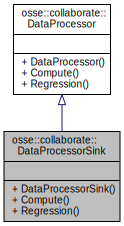
\includegraphics[width=207pt]{classosse_1_1collaborate_1_1_data_processor_sink__inherit__graph}
\end{center}
\end{figure}
\subsubsection*{Public Member Functions}
\begin{DoxyCompactItemize}
\item 
\mbox{\Hypertarget{classosse_1_1collaborate_1_1_data_processor_sink_a8d89873658f5237e951d066ecfdf1c37}\label{classosse_1_1collaborate_1_1_data_processor_sink_a8d89873658f5237e951d066ecfdf1c37}} 
\hyperlink{classosse_1_1collaborate_1_1_data_processor_sink_a8d89873658f5237e951d066ecfdf1c37}{Data\+Processor\+Sink} ()
\begin{DoxyCompactList}\small\item\em Constructor. \end{DoxyCompactList}\item 
void \hyperlink{classosse_1_1collaborate_1_1_data_processor_sink_a42b27e2e378f110add6f55406bdbfdd4}{Compute} (const std\+::vector$<$ \hyperlink{classosse_1_1collaborate_1_1_packet_raw}{Packet\+Raw} $>$ \&\+\_\+raw\+\_\+packets, const uint16\+\_\+t \&\+\_\+source\+\_\+index, const \hyperlink{classosse_1_1collaborate_1_1_simulation_clock}{Simulation\+Clock} \&\+\_\+clock, std\+::vector$<$ \hyperlink{classosse_1_1collaborate_1_1_geodetic}{Geodetic} $>$ $\ast$\+\_\+min\+\_\+list, std\+::vector$<$ \hyperlink{classosse_1_1collaborate_1_1_geodetic}{Geodetic} $>$ $\ast$\+\_\+max\+\_\+list, std\+::vector$<$ std\+::pair$<$ bool, uint16\+\_\+t $>$$>$ $\ast$\+\_\+feedback) const
\begin{DoxyCompactList}\small\item\em Processes a sensor measurement. \end{DoxyCompactList}\item 
void \hyperlink{classosse_1_1collaborate_1_1_data_processor_sink_a6f6dce42dffb76a6218f8d2be8bae9c4}{Regression} (const bool \&\+\_\+success, const uint16\+\_\+t \&\+\_\+constellation)
\begin{DoxyCompactList}\small\item\em Adapts thresholds in response to feedback. \end{DoxyCompactList}\end{DoxyCompactItemize}


\subsubsection{Detailed Description}
A sink satellite\textquotesingle{}s internal data processor. 

\subsubsection{Member Function Documentation}
\mbox{\Hypertarget{classosse_1_1collaborate_1_1_data_processor_sink_a42b27e2e378f110add6f55406bdbfdd4}\label{classosse_1_1collaborate_1_1_data_processor_sink_a42b27e2e378f110add6f55406bdbfdd4}} 
\index{osse\+::collaborate\+::\+Data\+Processor\+Sink@{osse\+::collaborate\+::\+Data\+Processor\+Sink}!Compute@{Compute}}
\index{Compute@{Compute}!osse\+::collaborate\+::\+Data\+Processor\+Sink@{osse\+::collaborate\+::\+Data\+Processor\+Sink}}
\paragraph{\texorpdfstring{Compute()}{Compute()}}
{\footnotesize\ttfamily void osse\+::collaborate\+::\+Data\+Processor\+Sink\+::\+Compute (\begin{DoxyParamCaption}\item[{const std\+::vector$<$ \hyperlink{classosse_1_1collaborate_1_1_packet_raw}{Packet\+Raw} $>$ \&}]{\+\_\+raw\+\_\+packets,  }\item[{const uint16\+\_\+t \&}]{\+\_\+source\+\_\+index,  }\item[{const \hyperlink{classosse_1_1collaborate_1_1_simulation_clock}{Simulation\+Clock} \&}]{\+\_\+clock,  }\item[{std\+::vector$<$ \hyperlink{classosse_1_1collaborate_1_1_geodetic}{Geodetic} $>$ $\ast$}]{\+\_\+min\+\_\+list,  }\item[{std\+::vector$<$ \hyperlink{classosse_1_1collaborate_1_1_geodetic}{Geodetic} $>$ $\ast$}]{\+\_\+max\+\_\+list,  }\item[{std\+::vector$<$ std\+::pair$<$ bool, uint16\+\_\+t $>$$>$ $\ast$}]{\+\_\+feedback }\end{DoxyParamCaption}) const\hspace{0.3cm}{\ttfamily [virtual]}}



Processes a sensor measurement. 


\begin{DoxyParams}[1]{Parameters}
\mbox{\tt in}  & {\em \+\_\+raw\+\_\+packets} & List of raw measurement packets \\
\hline
\mbox{\tt in}  & {\em \+\_\+source\+\_\+index} & Index of source node \\
\hline
\mbox{\tt in}  & {\em \+\_\+clock} & Simulation clock \\
\hline
\mbox{\tt in}  & {\em \+\_\+min\+\_\+list} & List of minimal suggestions \\
\hline
\mbox{\tt in}  & {\em \+\_\+max\+\_\+list} & List of maximum suggestions \\
\hline
\mbox{\tt in}  & {\em \+\_\+feedback} & List of feedback target node indices \\
\hline
\end{DoxyParams}


Implements \hyperlink{classosse_1_1collaborate_1_1_data_processor_af984306eb4619e7d5823a7293fe568cb}{osse\+::collaborate\+::\+Data\+Processor}.

\mbox{\Hypertarget{classosse_1_1collaborate_1_1_data_processor_sink_a6f6dce42dffb76a6218f8d2be8bae9c4}\label{classosse_1_1collaborate_1_1_data_processor_sink_a6f6dce42dffb76a6218f8d2be8bae9c4}} 
\index{osse\+::collaborate\+::\+Data\+Processor\+Sink@{osse\+::collaborate\+::\+Data\+Processor\+Sink}!Regression@{Regression}}
\index{Regression@{Regression}!osse\+::collaborate\+::\+Data\+Processor\+Sink@{osse\+::collaborate\+::\+Data\+Processor\+Sink}}
\paragraph{\texorpdfstring{Regression()}{Regression()}}
{\footnotesize\ttfamily void osse\+::collaborate\+::\+Data\+Processor\+Sink\+::\+Regression (\begin{DoxyParamCaption}\item[{const bool \&}]{\+\_\+success,  }\item[{const uint16\+\_\+t \&}]{\+\_\+constellation }\end{DoxyParamCaption})\hspace{0.3cm}{\ttfamily [virtual]}}



Adapts thresholds in response to feedback. 


\begin{DoxyParams}[1]{Parameters}
\mbox{\tt in}  & {\em \+\_\+success} & Whether the measurement exceeded the threshold \\
\hline
\mbox{\tt in}  & {\em \+\_\+constellation} & Constellation of the target satellite \\
\hline
\end{DoxyParams}


Implements \hyperlink{classosse_1_1collaborate_1_1_data_processor_a4efa75369a65d2a6011093facfcac44a}{osse\+::collaborate\+::\+Data\+Processor}.



The documentation for this class was generated from the following files\+:\begin{DoxyCompactItemize}
\item 
libs/collaborate/include/collaborate/data\+\_\+processor\+\_\+sink.\+h\item 
libs/collaborate/src/data\+\_\+processor\+\_\+sink.\+cpp\end{DoxyCompactItemize}

\hypertarget{classosse_1_1collaborate_1_1_data_processor_source}{}\subsection{osse\+:\+:collaborate\+:\+:Data\+Processor\+Source Class Reference}
\label{classosse_1_1collaborate_1_1_data_processor_source}\index{osse\+::collaborate\+::\+Data\+Processor\+Source@{osse\+::collaborate\+::\+Data\+Processor\+Source}}


A source/informer satellite\textquotesingle{}s internal data processor.  




{\ttfamily \#include $<$data\+\_\+processor\+\_\+source.\+h$>$}



Inheritance diagram for osse\+:\+:collaborate\+:\+:Data\+Processor\+Source\+:
\nopagebreak
\begin{figure}[H]
\begin{center}
\leavevmode
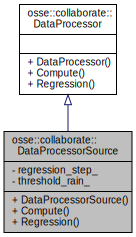
\includegraphics[width=219pt]{classosse_1_1collaborate_1_1_data_processor_source__inherit__graph}
\end{center}
\end{figure}
\subsubsection*{Public Member Functions}
\begin{DoxyCompactItemize}
\item 
\mbox{\Hypertarget{classosse_1_1collaborate_1_1_data_processor_source_abda2d1b8e2939b332b1690ea1bbd2e21}\label{classosse_1_1collaborate_1_1_data_processor_source_abda2d1b8e2939b332b1690ea1bbd2e21}} 
\hyperlink{classosse_1_1collaborate_1_1_data_processor_source_abda2d1b8e2939b332b1690ea1bbd2e21}{Data\+Processor\+Source} ()
\begin{DoxyCompactList}\small\item\em Constructor. \end{DoxyCompactList}\item 
\mbox{\Hypertarget{classosse_1_1collaborate_1_1_data_processor_source_af72b963c9cbf47f265e5f8deb4ec098f}\label{classosse_1_1collaborate_1_1_data_processor_source_af72b963c9cbf47f265e5f8deb4ec098f}} 
\hyperlink{classosse_1_1collaborate_1_1_data_processor_source_af72b963c9cbf47f265e5f8deb4ec098f}{Data\+Processor\+Source} (const bool \&\+\_\+flag)
\begin{DoxyCompactList}\small\item\em Constructor. \end{DoxyCompactList}\item 
void \hyperlink{classosse_1_1collaborate_1_1_data_processor_source_a625d453c95bf1491290afdd0b85d4681}{Compute} (const std\+::vector$<$ \hyperlink{classosse_1_1collaborate_1_1_packet_raw}{Packet\+Raw} $>$ \&\+\_\+raw\+\_\+packets, const uint16\+\_\+t \&\+\_\+source\+\_\+index, const \hyperlink{classosse_1_1collaborate_1_1_simulation_clock}{Simulation\+Clock} \&\+\_\+clock, std\+::vector$<$ \hyperlink{classosse_1_1collaborate_1_1_geodetic}{Geodetic} $>$ $\ast$\+\_\+min\+\_\+list, std\+::vector$<$ \hyperlink{classosse_1_1collaborate_1_1_geodetic}{Geodetic} $>$ $\ast$\+\_\+max\+\_\+list, std\+::vector$<$ std\+::pair$<$ bool, uint16\+\_\+t $>$$>$ $\ast$\+\_\+feedback) const
\begin{DoxyCompactList}\small\item\em Processes a sensor measurement. \end{DoxyCompactList}\item 
void \hyperlink{classosse_1_1collaborate_1_1_data_processor_source_ae9b24ff12942f0c667064a349d12fa9b}{Regression} (const bool \&\+\_\+success, const uint16\+\_\+t \&\+\_\+constellation)
\begin{DoxyCompactList}\small\item\em Adapts thresholds in response to feedback. \end{DoxyCompactList}\end{DoxyCompactItemize}
\subsubsection*{Private Attributes}
\begin{DoxyCompactItemize}
\item 
\mbox{\Hypertarget{classosse_1_1collaborate_1_1_data_processor_source_a676104998e0edb31c85f3ace7408ea30}\label{classosse_1_1collaborate_1_1_data_processor_source_a676104998e0edb31c85f3ace7408ea30}} 
double \hyperlink{classosse_1_1collaborate_1_1_data_processor_source_a676104998e0edb31c85f3ace7408ea30}{regression\+\_\+step\+\_\+}
\begin{DoxyCompactList}\small\item\em Size of correction in regression action. \end{DoxyCompactList}\item 
\mbox{\Hypertarget{classosse_1_1collaborate_1_1_data_processor_source_a987bff6789aae12fa88d317347304beb}\label{classosse_1_1collaborate_1_1_data_processor_source_a987bff6789aae12fa88d317347304beb}} 
double \hyperlink{classosse_1_1collaborate_1_1_data_processor_source_a987bff6789aae12fa88d317347304beb}{threshold\+\_\+rain\+\_\+}
\begin{DoxyCompactList}\small\item\em Cloud depth minimum for existence of rain. \end{DoxyCompactList}\item 
\mbox{\Hypertarget{classosse_1_1collaborate_1_1_data_processor_source_a9644f1ea065308146c05106d13dc2ccc}\label{classosse_1_1collaborate_1_1_data_processor_source_a9644f1ea065308146c05106d13dc2ccc}} 
bool \hyperlink{classosse_1_1collaborate_1_1_data_processor_source_a9644f1ea065308146c05106d13dc2ccc}{flag\+\_\+}
\begin{DoxyCompactList}\small\item\em Flag. \end{DoxyCompactList}\end{DoxyCompactItemize}


\subsubsection{Detailed Description}
A source/informer satellite\textquotesingle{}s internal data processor. 

\subsubsection{Member Function Documentation}
\mbox{\Hypertarget{classosse_1_1collaborate_1_1_data_processor_source_a625d453c95bf1491290afdd0b85d4681}\label{classosse_1_1collaborate_1_1_data_processor_source_a625d453c95bf1491290afdd0b85d4681}} 
\index{osse\+::collaborate\+::\+Data\+Processor\+Source@{osse\+::collaborate\+::\+Data\+Processor\+Source}!Compute@{Compute}}
\index{Compute@{Compute}!osse\+::collaborate\+::\+Data\+Processor\+Source@{osse\+::collaborate\+::\+Data\+Processor\+Source}}
\paragraph{\texorpdfstring{Compute()}{Compute()}}
{\footnotesize\ttfamily void osse\+::collaborate\+::\+Data\+Processor\+Source\+::\+Compute (\begin{DoxyParamCaption}\item[{const std\+::vector$<$ \hyperlink{classosse_1_1collaborate_1_1_packet_raw}{Packet\+Raw} $>$ \&}]{\+\_\+raw\+\_\+packets,  }\item[{const uint16\+\_\+t \&}]{\+\_\+source\+\_\+index,  }\item[{const \hyperlink{classosse_1_1collaborate_1_1_simulation_clock}{Simulation\+Clock} \&}]{\+\_\+clock,  }\item[{std\+::vector$<$ \hyperlink{classosse_1_1collaborate_1_1_geodetic}{Geodetic} $>$ $\ast$}]{\+\_\+min\+\_\+list,  }\item[{std\+::vector$<$ \hyperlink{classosse_1_1collaborate_1_1_geodetic}{Geodetic} $>$ $\ast$}]{\+\_\+max\+\_\+list,  }\item[{std\+::vector$<$ std\+::pair$<$ bool, uint16\+\_\+t $>$$>$ $\ast$}]{\+\_\+feedback }\end{DoxyParamCaption}) const\hspace{0.3cm}{\ttfamily [virtual]}}



Processes a sensor measurement. 


\begin{DoxyParams}[1]{Parameters}
\mbox{\tt in}  & {\em \+\_\+raw\+\_\+packets} & List of raw measurement packets \\
\hline
\mbox{\tt in}  & {\em \+\_\+source\+\_\+index} & Index of source node \\
\hline
\mbox{\tt in}  & {\em \+\_\+clock} & Simulation clock \\
\hline
\mbox{\tt in}  & {\em \+\_\+min\+\_\+list} & List of minimal suggestions \\
\hline
\mbox{\tt in}  & {\em \+\_\+max\+\_\+list} & List of maximum suggestions \\
\hline
\mbox{\tt in}  & {\em \+\_\+feedback} & List of feedback target node indices \\
\hline
\end{DoxyParams}


Implements \hyperlink{classosse_1_1collaborate_1_1_data_processor_af984306eb4619e7d5823a7293fe568cb}{osse\+::collaborate\+::\+Data\+Processor}.

\mbox{\Hypertarget{classosse_1_1collaborate_1_1_data_processor_source_ae9b24ff12942f0c667064a349d12fa9b}\label{classosse_1_1collaborate_1_1_data_processor_source_ae9b24ff12942f0c667064a349d12fa9b}} 
\index{osse\+::collaborate\+::\+Data\+Processor\+Source@{osse\+::collaborate\+::\+Data\+Processor\+Source}!Regression@{Regression}}
\index{Regression@{Regression}!osse\+::collaborate\+::\+Data\+Processor\+Source@{osse\+::collaborate\+::\+Data\+Processor\+Source}}
\paragraph{\texorpdfstring{Regression()}{Regression()}}
{\footnotesize\ttfamily void osse\+::collaborate\+::\+Data\+Processor\+Source\+::\+Regression (\begin{DoxyParamCaption}\item[{const bool \&}]{\+\_\+success,  }\item[{const uint16\+\_\+t \&}]{\+\_\+constellation }\end{DoxyParamCaption})\hspace{0.3cm}{\ttfamily [virtual]}}



Adapts thresholds in response to feedback. 


\begin{DoxyParams}[1]{Parameters}
\mbox{\tt in}  & {\em \+\_\+success} & Whether the measurement exceeded the threshold \\
\hline
\mbox{\tt in}  & {\em \+\_\+constellation} & Constellation of the target satellite \\
\hline
\end{DoxyParams}


Implements \hyperlink{classosse_1_1collaborate_1_1_data_processor_a4efa75369a65d2a6011093facfcac44a}{osse\+::collaborate\+::\+Data\+Processor}.



The documentation for this class was generated from the following files\+:\begin{DoxyCompactItemize}
\item 
libs/collaborate/include/collaborate/data\+\_\+processor\+\_\+source.\+h\item 
libs/collaborate/src/data\+\_\+processor\+\_\+source.\+cpp\end{DoxyCompactItemize}

\hypertarget{classosse_1_1collaborate_1_1_data_processor_template}{}\subsection{osse\+:\+:collaborate\+:\+:Data\+Processor\+Template Class Reference}
\label{classosse_1_1collaborate_1_1_data_processor_template}\index{osse\+::collaborate\+::\+Data\+Processor\+Template@{osse\+::collaborate\+::\+Data\+Processor\+Template}}


A template satellite\textquotesingle{}s internal data processor.  




{\ttfamily \#include $<$data\+\_\+processor\+\_\+template.\+h$>$}



Inheritance diagram for osse\+:\+:collaborate\+:\+:Data\+Processor\+Template\+:
\nopagebreak
\begin{figure}[H]
\begin{center}
\leavevmode
\includegraphics[width=231pt]{classosse_1_1collaborate_1_1_data_processor_template__inherit__graph}
\end{center}
\end{figure}
\subsubsection*{Public Member Functions}
\begin{DoxyCompactItemize}
\item 
\mbox{\Hypertarget{classosse_1_1collaborate_1_1_data_processor_template_ad4b855d7eb850e218b367c87e481bcd7}\label{classosse_1_1collaborate_1_1_data_processor_template_ad4b855d7eb850e218b367c87e481bcd7}} 
\hyperlink{classosse_1_1collaborate_1_1_data_processor_template_ad4b855d7eb850e218b367c87e481bcd7}{Data\+Processor\+Template} ()
\begin{DoxyCompactList}\small\item\em Constructor. \end{DoxyCompactList}\item 
void \hyperlink{classosse_1_1collaborate_1_1_data_processor_template_a01a3532d55daf656a30232dab91e293e}{Compute} (const std\+::vector$<$ \hyperlink{classosse_1_1collaborate_1_1_packet_raw}{Packet\+Raw} $>$ \&\+\_\+raw\+\_\+packets, const uint16\+\_\+t \&\+\_\+source\+\_\+index, const \hyperlink{classosse_1_1collaborate_1_1_simulation_clock}{Simulation\+Clock} \&\+\_\+simulation\+\_\+clock, std\+::vector$<$ \hyperlink{classosse_1_1collaborate_1_1_geodetic}{Geodetic} $>$ $\ast$\+\_\+min\+\_\+list, std\+::vector$<$ \hyperlink{classosse_1_1collaborate_1_1_geodetic}{Geodetic} $>$ $\ast$\+\_\+max\+\_\+list, std\+::vector$<$ std\+::pair$<$ bool, uint16\+\_\+t $>$$>$ $\ast$\+\_\+feedback) const
\begin{DoxyCompactList}\small\item\em Processes a sensor measurement. \end{DoxyCompactList}\item 
void \hyperlink{classosse_1_1collaborate_1_1_data_processor_template_a3cf1401b98a7e06852f3f46d464308ea}{Regression} (const bool \&\+\_\+success, const uint16\+\_\+t \&\+\_\+constellation)
\begin{DoxyCompactList}\small\item\em Adapts thresholds in response to feedback. \end{DoxyCompactList}\end{DoxyCompactItemize}


\subsubsection{Detailed Description}
A template satellite\textquotesingle{}s internal data processor. 

\subsubsection{Member Function Documentation}
\mbox{\Hypertarget{classosse_1_1collaborate_1_1_data_processor_template_a01a3532d55daf656a30232dab91e293e}\label{classosse_1_1collaborate_1_1_data_processor_template_a01a3532d55daf656a30232dab91e293e}} 
\index{osse\+::collaborate\+::\+Data\+Processor\+Template@{osse\+::collaborate\+::\+Data\+Processor\+Template}!Compute@{Compute}}
\index{Compute@{Compute}!osse\+::collaborate\+::\+Data\+Processor\+Template@{osse\+::collaborate\+::\+Data\+Processor\+Template}}
\paragraph{\texorpdfstring{Compute()}{Compute()}}
{\footnotesize\ttfamily void osse\+::collaborate\+::\+Data\+Processor\+Template\+::\+Compute (\begin{DoxyParamCaption}\item[{const std\+::vector$<$ \hyperlink{classosse_1_1collaborate_1_1_packet_raw}{Packet\+Raw} $>$ \&}]{\+\_\+raw\+\_\+packets,  }\item[{const uint16\+\_\+t \&}]{\+\_\+source\+\_\+index,  }\item[{const \hyperlink{classosse_1_1collaborate_1_1_simulation_clock}{Simulation\+Clock} \&}]{\+\_\+simulation\+\_\+clock,  }\item[{std\+::vector$<$ \hyperlink{classosse_1_1collaborate_1_1_geodetic}{Geodetic} $>$ $\ast$}]{\+\_\+min\+\_\+list,  }\item[{std\+::vector$<$ \hyperlink{classosse_1_1collaborate_1_1_geodetic}{Geodetic} $>$ $\ast$}]{\+\_\+max\+\_\+list,  }\item[{std\+::vector$<$ std\+::pair$<$ bool, uint16\+\_\+t $>$$>$ $\ast$}]{\+\_\+feedback }\end{DoxyParamCaption}) const\hspace{0.3cm}{\ttfamily [virtual]}}



Processes a sensor measurement. 


\begin{DoxyParams}[1]{Parameters}
\mbox{\tt in}  & {\em \+\_\+raw\+\_\+packets} & List of raw measurement packets \\
\hline
\mbox{\tt in}  & {\em \+\_\+source\+\_\+index} & Index of source node \\
\hline
\mbox{\tt in}  & {\em \+\_\+simulation\+\_\+clock} & Simulation simulation\+\_\+clock \\
\hline
\mbox{\tt in}  & {\em \+\_\+min\+\_\+list} & List of minimal suggestions \\
\hline
\mbox{\tt in}  & {\em \+\_\+max\+\_\+list} & List of minimal suggestions \\
\hline
\mbox{\tt in}  & {\em \+\_\+feedback} & List of feedback target node indices \\
\hline
\end{DoxyParams}


Implements \hyperlink{classosse_1_1collaborate_1_1_data_processor_af984306eb4619e7d5823a7293fe568cb}{osse\+::collaborate\+::\+Data\+Processor}.

\mbox{\Hypertarget{classosse_1_1collaborate_1_1_data_processor_template_a3cf1401b98a7e06852f3f46d464308ea}\label{classosse_1_1collaborate_1_1_data_processor_template_a3cf1401b98a7e06852f3f46d464308ea}} 
\index{osse\+::collaborate\+::\+Data\+Processor\+Template@{osse\+::collaborate\+::\+Data\+Processor\+Template}!Regression@{Regression}}
\index{Regression@{Regression}!osse\+::collaborate\+::\+Data\+Processor\+Template@{osse\+::collaborate\+::\+Data\+Processor\+Template}}
\paragraph{\texorpdfstring{Regression()}{Regression()}}
{\footnotesize\ttfamily void osse\+::collaborate\+::\+Data\+Processor\+Template\+::\+Regression (\begin{DoxyParamCaption}\item[{const bool \&}]{\+\_\+success,  }\item[{const uint16\+\_\+t \&}]{\+\_\+constellation }\end{DoxyParamCaption})\hspace{0.3cm}{\ttfamily [virtual]}}



Adapts thresholds in response to feedback. 


\begin{DoxyParams}[1]{Parameters}
\mbox{\tt in}  & {\em \+\_\+success} & Whether the measurement exceeded the threshold \\
\hline
\mbox{\tt in}  & {\em \+\_\+constellation} & Constellation of the target satellite \\
\hline
\end{DoxyParams}


Implements \hyperlink{classosse_1_1collaborate_1_1_data_processor_a4efa75369a65d2a6011093facfcac44a}{osse\+::collaborate\+::\+Data\+Processor}.



The documentation for this class was generated from the following files\+:\begin{DoxyCompactItemize}
\item 
libs/collaborate/include/collaborate/data\+\_\+processor\+\_\+template.\+h\item 
libs/collaborate/src/data\+\_\+processor\+\_\+template.\+cpp\end{DoxyCompactItemize}

\hypertarget{classosse_1_1collaborate_1_1_data_processor}{}\subsection{osse\+:\+:collaborate\+:\+:Data\+Processor Class Reference}
\label{classosse_1_1collaborate_1_1_data_processor}\index{osse\+::collaborate\+::\+Data\+Processor@{osse\+::collaborate\+::\+Data\+Processor}}


A satellite\textquotesingle{}s internal data processor.  




{\ttfamily \#include $<$data\+\_\+processor.\+h$>$}



Inheritance diagram for osse\+:\+:collaborate\+:\+:Data\+Processor\+:
\nopagebreak
\begin{figure}[H]
\begin{center}
\leavevmode
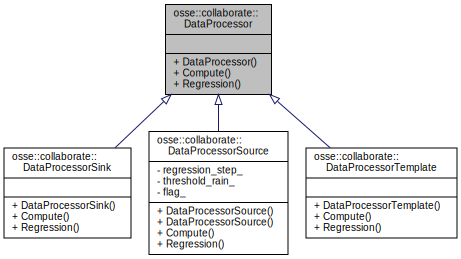
\includegraphics[width=350pt]{classosse_1_1collaborate_1_1_data_processor__inherit__graph}
\end{center}
\end{figure}
\subsubsection*{Public Member Functions}
\begin{DoxyCompactItemize}
\item 
\mbox{\Hypertarget{classosse_1_1collaborate_1_1_data_processor_ac967fe6b10b12e0eede67fc26001202e}\label{classosse_1_1collaborate_1_1_data_processor_ac967fe6b10b12e0eede67fc26001202e}} 
\hyperlink{classosse_1_1collaborate_1_1_data_processor_ac967fe6b10b12e0eede67fc26001202e}{Data\+Processor} ()
\begin{DoxyCompactList}\small\item\em Constructor. \end{DoxyCompactList}\item 
virtual void \hyperlink{classosse_1_1collaborate_1_1_data_processor_af984306eb4619e7d5823a7293fe568cb}{Compute} (const std\+::vector$<$ \hyperlink{classosse_1_1collaborate_1_1_packet_raw}{Packet\+Raw} $>$ \&\+\_\+raw\+\_\+packets, const uint16\+\_\+t \&\+\_\+source\+\_\+index, const \hyperlink{classosse_1_1collaborate_1_1_simulation_clock}{Simulation\+Clock} \&\+\_\+clock, std\+::vector$<$ \hyperlink{classosse_1_1collaborate_1_1_geodetic}{Geodetic} $>$ $\ast$\+\_\+min\+\_\+list, std\+::vector$<$ \hyperlink{classosse_1_1collaborate_1_1_geodetic}{Geodetic} $>$ $\ast$\+\_\+max\+\_\+list, std\+::vector$<$ std\+::pair$<$ bool, uint16\+\_\+t $>$$>$ $\ast$\+\_\+feedback) const =0
\begin{DoxyCompactList}\small\item\em Processes a sensor measurement. \end{DoxyCompactList}\item 
virtual void \hyperlink{classosse_1_1collaborate_1_1_data_processor_a4efa75369a65d2a6011093facfcac44a}{Regression} (const bool \&\+\_\+success, const uint16\+\_\+t \&\+\_\+constellation)=0
\begin{DoxyCompactList}\small\item\em Adapts thresholds in response to feedback. \end{DoxyCompactList}\end{DoxyCompactItemize}


\subsubsection{Detailed Description}
A satellite\textquotesingle{}s internal data processor. 

\subsubsection{Member Function Documentation}
\mbox{\Hypertarget{classosse_1_1collaborate_1_1_data_processor_af984306eb4619e7d5823a7293fe568cb}\label{classosse_1_1collaborate_1_1_data_processor_af984306eb4619e7d5823a7293fe568cb}} 
\index{osse\+::collaborate\+::\+Data\+Processor@{osse\+::collaborate\+::\+Data\+Processor}!Compute@{Compute}}
\index{Compute@{Compute}!osse\+::collaborate\+::\+Data\+Processor@{osse\+::collaborate\+::\+Data\+Processor}}
\paragraph{\texorpdfstring{Compute()}{Compute()}}
{\footnotesize\ttfamily virtual void osse\+::collaborate\+::\+Data\+Processor\+::\+Compute (\begin{DoxyParamCaption}\item[{const std\+::vector$<$ \hyperlink{classosse_1_1collaborate_1_1_packet_raw}{Packet\+Raw} $>$ \&}]{\+\_\+raw\+\_\+packets,  }\item[{const uint16\+\_\+t \&}]{\+\_\+source\+\_\+index,  }\item[{const \hyperlink{classosse_1_1collaborate_1_1_simulation_clock}{Simulation\+Clock} \&}]{\+\_\+clock,  }\item[{std\+::vector$<$ \hyperlink{classosse_1_1collaborate_1_1_geodetic}{Geodetic} $>$ $\ast$}]{\+\_\+min\+\_\+list,  }\item[{std\+::vector$<$ \hyperlink{classosse_1_1collaborate_1_1_geodetic}{Geodetic} $>$ $\ast$}]{\+\_\+max\+\_\+list,  }\item[{std\+::vector$<$ std\+::pair$<$ bool, uint16\+\_\+t $>$$>$ $\ast$}]{\+\_\+feedback }\end{DoxyParamCaption}) const\hspace{0.3cm}{\ttfamily [pure virtual]}}



Processes a sensor measurement. 


\begin{DoxyParams}[1]{Parameters}
\mbox{\tt in}  & {\em \+\_\+raw\+\_\+packets} & List of raw measurement packets \\
\hline
\mbox{\tt in}  & {\em \+\_\+source\+\_\+index} & Index of source node \\
\hline
\mbox{\tt in}  & {\em \+\_\+clock} & Simulation clock \\
\hline
\mbox{\tt in}  & {\em \+\_\+min\+\_\+list} & List of minimal suggestions \\
\hline
\mbox{\tt in}  & {\em \+\_\+max\+\_\+list} & List of maximum suggestions \\
\hline
\mbox{\tt in}  & {\em \+\_\+feedback} & List of feedback target node indices \\
\hline
\end{DoxyParams}


Implemented in \hyperlink{classosse_1_1collaborate_1_1_data_processor_source_a625d453c95bf1491290afdd0b85d4681}{osse\+::collaborate\+::\+Data\+Processor\+Source}, \hyperlink{classosse_1_1collaborate_1_1_data_processor_sink_a42b27e2e378f110add6f55406bdbfdd4}{osse\+::collaborate\+::\+Data\+Processor\+Sink}, and \hyperlink{classosse_1_1collaborate_1_1_data_processor_template_a01a3532d55daf656a30232dab91e293e}{osse\+::collaborate\+::\+Data\+Processor\+Template}.

\mbox{\Hypertarget{classosse_1_1collaborate_1_1_data_processor_a4efa75369a65d2a6011093facfcac44a}\label{classosse_1_1collaborate_1_1_data_processor_a4efa75369a65d2a6011093facfcac44a}} 
\index{osse\+::collaborate\+::\+Data\+Processor@{osse\+::collaborate\+::\+Data\+Processor}!Regression@{Regression}}
\index{Regression@{Regression}!osse\+::collaborate\+::\+Data\+Processor@{osse\+::collaborate\+::\+Data\+Processor}}
\paragraph{\texorpdfstring{Regression()}{Regression()}}
{\footnotesize\ttfamily virtual void osse\+::collaborate\+::\+Data\+Processor\+::\+Regression (\begin{DoxyParamCaption}\item[{const bool \&}]{\+\_\+success,  }\item[{const uint16\+\_\+t \&}]{\+\_\+constellation }\end{DoxyParamCaption})\hspace{0.3cm}{\ttfamily [pure virtual]}}



Adapts thresholds in response to feedback. 


\begin{DoxyParams}[1]{Parameters}
\mbox{\tt in}  & {\em \+\_\+success} & Whether the measurement exceeded the threshold \\
\hline
\mbox{\tt in}  & {\em \+\_\+constellation} & Constellation of the target satellite \\
\hline
\end{DoxyParams}


Implemented in \hyperlink{classosse_1_1collaborate_1_1_data_processor_source_ae9b24ff12942f0c667064a349d12fa9b}{osse\+::collaborate\+::\+Data\+Processor\+Source}, \hyperlink{classosse_1_1collaborate_1_1_data_processor_sink_a6f6dce42dffb76a6218f8d2be8bae9c4}{osse\+::collaborate\+::\+Data\+Processor\+Sink}, and \hyperlink{classosse_1_1collaborate_1_1_data_processor_template_a3cf1401b98a7e06852f3f46d464308ea}{osse\+::collaborate\+::\+Data\+Processor\+Template}.



The documentation for this class was generated from the following files\+:\begin{DoxyCompactItemize}
\item 
libs/collaborate/include/collaborate/data\+\_\+processor.\+h\item 
libs/collaborate/src/data\+\_\+processor.\+cpp\end{DoxyCompactItemize}

\hypertarget{classosse_1_1collaborate_1_1_earth_data}{}\subsection{osse\+:\+:collaborate\+:\+:Earth\+Data Class Reference}
\label{classosse_1_1collaborate_1_1_earth_data}\index{osse\+::collaborate\+::\+Earth\+Data@{osse\+::collaborate\+::\+Earth\+Data}}


A map of scientific measurement data.  




{\ttfamily \#include $<$earth\+\_\+data.\+h$>$}

\subsubsection*{Public Member Functions}
\begin{DoxyCompactItemize}
\item 
\hyperlink{classosse_1_1collaborate_1_1_earth_data_a77ce398a29306b84cdddbd937cb62bbd}{Earth\+Data} (const std\+::string \&\+\_\+root)
\begin{DoxyCompactList}\small\item\em Constructor. \end{DoxyCompactList}\item 
void \hyperlink{classosse_1_1collaborate_1_1_earth_data_a22d7fe03f04f1b3b10020271b16dec5c}{Update} (const \hyperlink{classosse_1_1collaborate_1_1_simulation_clock}{Simulation\+Clock} \&\+\_\+clock, const std\+::string \&\+\_\+variable)
\begin{DoxyCompactList}\small\item\em Updates the truth data with a new frame of measurement data. \end{DoxyCompactList}\item 
float \hyperlink{classosse_1_1collaborate_1_1_earth_data_a39c94ce236efd3ddb85e6108205a7067}{Measure} (const double \&\+\_\+latitude\+\_\+rad, const double \&\+\_\+longitude\+\_\+rad) const
\begin{DoxyCompactList}\small\item\em Obtains a data sample at the nearest location on the discrete map. \end{DoxyCompactList}\end{DoxyCompactItemize}
\subsubsection*{Private Member Functions}
\begin{DoxyCompactItemize}
\item 
void \hyperlink{classosse_1_1collaborate_1_1_earth_data_a7a00924ea65a5ea68c25fbba2c1d3c9d}{Buffer} (const std\+::string \&\+\_\+variable)
\begin{DoxyCompactList}\small\item\em Loads netcdf data into the current data frame. \end{DoxyCompactList}\item 
uint16\+\_\+t \hyperlink{classosse_1_1collaborate_1_1_earth_data_a5c22945fb816aac16410d2641bba666c}{Index\+Latitude} (const double \&\+\_\+latitude\+\_\+rad) const
\begin{DoxyCompactList}\small\item\em Obtains the index of the nearest latitude value. \end{DoxyCompactList}\item 
uint16\+\_\+t \hyperlink{classosse_1_1collaborate_1_1_earth_data_affbe14ade774253ba546982953996574}{Index\+Longitude} (const double \&\+\_\+longitude\+\_\+rad) const
\begin{DoxyCompactList}\small\item\em Obtains the index of the nearest longitude value. \end{DoxyCompactList}\item 
std\+::vector$<$ std\+::string $>$ \hyperlink{classosse_1_1collaborate_1_1_earth_data_ab97521a1742be97c74a0aa538f8ad180}{Find\+Data\+Paths} (const std\+::string \&\+\_\+root) const
\begin{DoxyCompactList}\small\item\em Finds all regular paths in a directory. \end{DoxyCompactList}\end{DoxyCompactItemize}
\subsubsection*{Private Attributes}
\begin{DoxyCompactItemize}
\item 
\mbox{\Hypertarget{classosse_1_1collaborate_1_1_earth_data_aec97d6b176f78cc12e94038ca93234ba}\label{classosse_1_1collaborate_1_1_earth_data_aec97d6b176f78cc12e94038ca93234ba}} 
const std\+::vector$<$ std\+::string $>$ \hyperlink{classosse_1_1collaborate_1_1_earth_data_aec97d6b176f78cc12e94038ca93234ba}{data\+\_\+paths\+\_\+}
\begin{DoxyCompactList}\small\item\em The list of netcdf files. \end{DoxyCompactList}\item 
\mbox{\Hypertarget{classosse_1_1collaborate_1_1_earth_data_ad6b69b9ff9d275e6546fd940c0a9d21c}\label{classosse_1_1collaborate_1_1_earth_data_ad6b69b9ff9d275e6546fd940c0a9d21c}} 
uint64\+\_\+t \hyperlink{classosse_1_1collaborate_1_1_earth_data_ad6b69b9ff9d275e6546fd940c0a9d21c}{current\+\_\+index\+\_\+}
\begin{DoxyCompactList}\small\item\em Current data-\/set\textquotesingle{}s index. \end{DoxyCompactList}\item 
\mbox{\Hypertarget{classosse_1_1collaborate_1_1_earth_data_a8a2c4b1c349e08640731dc8062a83fe7}\label{classosse_1_1collaborate_1_1_earth_data_a8a2c4b1c349e08640731dc8062a83fe7}} 
std\+::array$<$ float, earth\+::k\+Num\+Positions $>$ \hyperlink{classosse_1_1collaborate_1_1_earth_data_a8a2c4b1c349e08640731dc8062a83fe7}{k\+Data\+\_\+}
\begin{DoxyCompactList}\small\item\em Current data set. \end{DoxyCompactList}\end{DoxyCompactItemize}


\subsubsection{Detailed Description}
A map of scientific measurement data. 

 
\begin{DoxyImageNoCaption}
  \mbox{\includegraphics[width=\textwidth]{combined}}
\end{DoxyImageNoCaption}
 

\subsubsection{Constructor \& Destructor Documentation}
\mbox{\Hypertarget{classosse_1_1collaborate_1_1_earth_data_a77ce398a29306b84cdddbd937cb62bbd}\label{classosse_1_1collaborate_1_1_earth_data_a77ce398a29306b84cdddbd937cb62bbd}} 
\index{osse\+::collaborate\+::\+Earth\+Data@{osse\+::collaborate\+::\+Earth\+Data}!Earth\+Data@{Earth\+Data}}
\index{Earth\+Data@{Earth\+Data}!osse\+::collaborate\+::\+Earth\+Data@{osse\+::collaborate\+::\+Earth\+Data}}
\paragraph{\texorpdfstring{Earth\+Data()}{EarthData()}}
{\footnotesize\ttfamily osse\+::collaborate\+::\+Earth\+Data\+::\+Earth\+Data (\begin{DoxyParamCaption}\item[{const std\+::string \&}]{\+\_\+root }\end{DoxyParamCaption})\hspace{0.3cm}{\ttfamily [explicit]}}



Constructor. 


\begin{DoxyParams}[1]{Parameters}
\mbox{\tt in}  & {\em \+\_\+root} & Root directory path \\
\hline
\end{DoxyParams}


\subsubsection{Member Function Documentation}
\mbox{\Hypertarget{classosse_1_1collaborate_1_1_earth_data_a7a00924ea65a5ea68c25fbba2c1d3c9d}\label{classosse_1_1collaborate_1_1_earth_data_a7a00924ea65a5ea68c25fbba2c1d3c9d}} 
\index{osse\+::collaborate\+::\+Earth\+Data@{osse\+::collaborate\+::\+Earth\+Data}!Buffer@{Buffer}}
\index{Buffer@{Buffer}!osse\+::collaborate\+::\+Earth\+Data@{osse\+::collaborate\+::\+Earth\+Data}}
\paragraph{\texorpdfstring{Buffer()}{Buffer()}}
{\footnotesize\ttfamily void osse\+::collaborate\+::\+Earth\+Data\+::\+Buffer (\begin{DoxyParamCaption}\item[{const std\+::string \&}]{\+\_\+variable }\end{DoxyParamCaption})\hspace{0.3cm}{\ttfamily [private]}}



Loads netcdf data into the current data frame. 


\begin{DoxyParams}[1]{Parameters}
\mbox{\tt in}  & {\em \+\_\+variable} & Variable in nercdf file \\
\hline
\end{DoxyParams}
\mbox{\Hypertarget{classosse_1_1collaborate_1_1_earth_data_ab97521a1742be97c74a0aa538f8ad180}\label{classosse_1_1collaborate_1_1_earth_data_ab97521a1742be97c74a0aa538f8ad180}} 
\index{osse\+::collaborate\+::\+Earth\+Data@{osse\+::collaborate\+::\+Earth\+Data}!Find\+Data\+Paths@{Find\+Data\+Paths}}
\index{Find\+Data\+Paths@{Find\+Data\+Paths}!osse\+::collaborate\+::\+Earth\+Data@{osse\+::collaborate\+::\+Earth\+Data}}
\paragraph{\texorpdfstring{Find\+Data\+Paths()}{FindDataPaths()}}
{\footnotesize\ttfamily std\+::vector$<$ std\+::string $>$ osse\+::collaborate\+::\+Earth\+Data\+::\+Find\+Data\+Paths (\begin{DoxyParamCaption}\item[{const std\+::string \&}]{\+\_\+root }\end{DoxyParamCaption}) const\hspace{0.3cm}{\ttfamily [private]}}



Finds all regular paths in a directory. 


\begin{DoxyParams}[1]{Parameters}
\mbox{\tt in}  & {\em \+\_\+root} & Root directory path name \\
\hline
\end{DoxyParams}
\begin{DoxyReturn}{Returns}
List of all regular paths in a directory 
\end{DoxyReturn}
\mbox{\Hypertarget{classosse_1_1collaborate_1_1_earth_data_a5c22945fb816aac16410d2641bba666c}\label{classosse_1_1collaborate_1_1_earth_data_a5c22945fb816aac16410d2641bba666c}} 
\index{osse\+::collaborate\+::\+Earth\+Data@{osse\+::collaborate\+::\+Earth\+Data}!Index\+Latitude@{Index\+Latitude}}
\index{Index\+Latitude@{Index\+Latitude}!osse\+::collaborate\+::\+Earth\+Data@{osse\+::collaborate\+::\+Earth\+Data}}
\paragraph{\texorpdfstring{Index\+Latitude()}{IndexLatitude()}}
{\footnotesize\ttfamily uint16\+\_\+t osse\+::collaborate\+::\+Earth\+Data\+::\+Index\+Latitude (\begin{DoxyParamCaption}\item[{const double \&}]{\+\_\+latitude\+\_\+rad }\end{DoxyParamCaption}) const\hspace{0.3cm}{\ttfamily [private]}}



Obtains the index of the nearest latitude value. 


\begin{DoxyParams}[1]{Parameters}
\mbox{\tt in}  & {\em \+\_\+latitude\+\_\+rad} & Latitude (radians) \\
\hline
\end{DoxyParams}
\begin{DoxyReturn}{Returns}
Index of the nearest latitude value 
\end{DoxyReturn}
\mbox{\Hypertarget{classosse_1_1collaborate_1_1_earth_data_affbe14ade774253ba546982953996574}\label{classosse_1_1collaborate_1_1_earth_data_affbe14ade774253ba546982953996574}} 
\index{osse\+::collaborate\+::\+Earth\+Data@{osse\+::collaborate\+::\+Earth\+Data}!Index\+Longitude@{Index\+Longitude}}
\index{Index\+Longitude@{Index\+Longitude}!osse\+::collaborate\+::\+Earth\+Data@{osse\+::collaborate\+::\+Earth\+Data}}
\paragraph{\texorpdfstring{Index\+Longitude()}{IndexLongitude()}}
{\footnotesize\ttfamily uint16\+\_\+t osse\+::collaborate\+::\+Earth\+Data\+::\+Index\+Longitude (\begin{DoxyParamCaption}\item[{const double \&}]{\+\_\+longitude\+\_\+rad }\end{DoxyParamCaption}) const\hspace{0.3cm}{\ttfamily [private]}}



Obtains the index of the nearest longitude value. 


\begin{DoxyParams}[1]{Parameters}
\mbox{\tt in}  & {\em \+\_\+longitude\+\_\+rad} & Longitude (radians) \\
\hline
\end{DoxyParams}
\begin{DoxyReturn}{Returns}
Index of the nearest longitude value 
\end{DoxyReturn}
\mbox{\Hypertarget{classosse_1_1collaborate_1_1_earth_data_a39c94ce236efd3ddb85e6108205a7067}\label{classosse_1_1collaborate_1_1_earth_data_a39c94ce236efd3ddb85e6108205a7067}} 
\index{osse\+::collaborate\+::\+Earth\+Data@{osse\+::collaborate\+::\+Earth\+Data}!Measure@{Measure}}
\index{Measure@{Measure}!osse\+::collaborate\+::\+Earth\+Data@{osse\+::collaborate\+::\+Earth\+Data}}
\paragraph{\texorpdfstring{Measure()}{Measure()}}
{\footnotesize\ttfamily float osse\+::collaborate\+::\+Earth\+Data\+::\+Measure (\begin{DoxyParamCaption}\item[{const double \&}]{\+\_\+latitude\+\_\+rad,  }\item[{const double \&}]{\+\_\+longitude\+\_\+rad }\end{DoxyParamCaption}) const}



Obtains a data sample at the nearest location on the discrete map. 


\begin{DoxyParams}[1]{Parameters}
\mbox{\tt in}  & {\em \+\_\+latitude\+\_\+rad} & Latitude (radians) \\
\hline
\mbox{\tt in}  & {\em \+\_\+longitude\+\_\+rad} & Longitude (radians) \\
\hline
\end{DoxyParams}
\begin{DoxyReturn}{Returns}
The data sample 
\end{DoxyReturn}
\mbox{\Hypertarget{classosse_1_1collaborate_1_1_earth_data_a22d7fe03f04f1b3b10020271b16dec5c}\label{classosse_1_1collaborate_1_1_earth_data_a22d7fe03f04f1b3b10020271b16dec5c}} 
\index{osse\+::collaborate\+::\+Earth\+Data@{osse\+::collaborate\+::\+Earth\+Data}!Update@{Update}}
\index{Update@{Update}!osse\+::collaborate\+::\+Earth\+Data@{osse\+::collaborate\+::\+Earth\+Data}}
\paragraph{\texorpdfstring{Update()}{Update()}}
{\footnotesize\ttfamily void osse\+::collaborate\+::\+Earth\+Data\+::\+Update (\begin{DoxyParamCaption}\item[{const \hyperlink{classosse_1_1collaborate_1_1_simulation_clock}{Simulation\+Clock} \&}]{\+\_\+clock,  }\item[{const std\+::string \&}]{\+\_\+variable }\end{DoxyParamCaption})}



Updates the truth data with a new frame of measurement data. 


\begin{DoxyParams}[1]{Parameters}
\mbox{\tt in}  & {\em \+\_\+clock} & Simulation clock \\
\hline
\mbox{\tt in}  & {\em \+\_\+variable} & Variable in nercdf file \\
\hline
\end{DoxyParams}


The documentation for this class was generated from the following files\+:\begin{DoxyCompactItemize}
\item 
libs/collaborate/include/collaborate/earth\+\_\+data.\+h\item 
libs/collaborate/src/earth\+\_\+data.\+cpp\end{DoxyCompactItemize}

\hypertarget{classosse_1_1collaborate_1_1_event_logger}{}\subsection{osse\+:\+:collaborate\+:\+:Event\+Logger Class Reference}
\label{classosse_1_1collaborate_1_1_event_logger}\index{osse\+::collaborate\+::\+Event\+Logger@{osse\+::collaborate\+::\+Event\+Logger}}


An interface to the spdlog logger.  




{\ttfamily \#include $<$event\+\_\+logger.\+h$>$}

\subsubsection*{Public Member Functions}
\begin{DoxyCompactItemize}
\item 
\hyperlink{classosse_1_1collaborate_1_1_event_logger_a9c87908de9f2673fe6464b59df4082d1}{Event\+Logger} (const std\+::string \&\+\_\+path)
\begin{DoxyCompactList}\small\item\em Constructor. \end{DoxyCompactList}\item 
void \hyperlink{classosse_1_1collaborate_1_1_event_logger_ad76479bfe7482caf22f6fd9e70445640}{Initialize} (const std\+::string \&\+\_\+level, const std\+::string \&\+\_\+console\+\_\+level, const bool \&\+\_\+utc)
\begin{DoxyCompactList}\small\item\em Initialize the event logger\textquotesingle{}s behavor. \end{DoxyCompactList}\item 
spdlog\+::logger $\ast$ \hyperlink{classosse_1_1collaborate_1_1_event_logger_a76adbd3cee03eb159797eb14dd496bc6}{log} ()
\begin{DoxyCompactList}\small\item\em Get the spdlog. \end{DoxyCompactList}\end{DoxyCompactItemize}
\subsubsection*{Private Attributes}
\begin{DoxyCompactItemize}
\item 
\mbox{\Hypertarget{classosse_1_1collaborate_1_1_event_logger_a251a1f450efb2a8b48689dff5056e8cd}\label{classosse_1_1collaborate_1_1_event_logger_a251a1f450efb2a8b48689dff5056e8cd}} 
std\+::shared\+\_\+ptr$<$ spdlog\+::sinks\+::stdout\+\_\+color\+\_\+sink\+\_\+mt $>$ \hyperlink{classosse_1_1collaborate_1_1_event_logger_a251a1f450efb2a8b48689dff5056e8cd}{console\+\_\+}
\begin{DoxyCompactList}\small\item\em Console sink. \end{DoxyCompactList}\item 
\mbox{\Hypertarget{classosse_1_1collaborate_1_1_event_logger_a42a6aa81525ec44dcee5b76d8a238e5b}\label{classosse_1_1collaborate_1_1_event_logger_a42a6aa81525ec44dcee5b76d8a238e5b}} 
std\+::shared\+\_\+ptr$<$ spdlog\+::sinks\+::basic\+\_\+file\+\_\+sink\+\_\+mt $>$ \hyperlink{classosse_1_1collaborate_1_1_event_logger_a42a6aa81525ec44dcee5b76d8a238e5b}{file\+\_\+}
\begin{DoxyCompactList}\small\item\em File sink. \end{DoxyCompactList}\item 
\mbox{\Hypertarget{classosse_1_1collaborate_1_1_event_logger_af5ebd14804c7ffd7a584e9a389d47f53}\label{classosse_1_1collaborate_1_1_event_logger_af5ebd14804c7ffd7a584e9a389d47f53}} 
std\+::unique\+\_\+ptr$<$ spdlog\+::logger $>$ \hyperlink{classosse_1_1collaborate_1_1_event_logger_af5ebd14804c7ffd7a584e9a389d47f53}{log\+\_\+}
\begin{DoxyCompactList}\small\item\em Multi-\/sink. \end{DoxyCompactList}\end{DoxyCompactItemize}


\subsubsection{Detailed Description}
An interface to the spdlog logger. 

\subsubsection{Constructor \& Destructor Documentation}
\mbox{\Hypertarget{classosse_1_1collaborate_1_1_event_logger_a9c87908de9f2673fe6464b59df4082d1}\label{classosse_1_1collaborate_1_1_event_logger_a9c87908de9f2673fe6464b59df4082d1}} 
\index{osse\+::collaborate\+::\+Event\+Logger@{osse\+::collaborate\+::\+Event\+Logger}!Event\+Logger@{Event\+Logger}}
\index{Event\+Logger@{Event\+Logger}!osse\+::collaborate\+::\+Event\+Logger@{osse\+::collaborate\+::\+Event\+Logger}}
\paragraph{\texorpdfstring{Event\+Logger()}{EventLogger()}}
{\footnotesize\ttfamily osse\+::collaborate\+::\+Event\+Logger\+::\+Event\+Logger (\begin{DoxyParamCaption}\item[{const std\+::string \&}]{\+\_\+path }\end{DoxyParamCaption})\hspace{0.3cm}{\ttfamily [explicit]}}



Constructor. 


\begin{DoxyParams}[1]{Parameters}
\mbox{\tt in}  & {\em \+\_\+path} & File sink path \\
\hline
\end{DoxyParams}


\subsubsection{Member Function Documentation}
\mbox{\Hypertarget{classosse_1_1collaborate_1_1_event_logger_ad76479bfe7482caf22f6fd9e70445640}\label{classosse_1_1collaborate_1_1_event_logger_ad76479bfe7482caf22f6fd9e70445640}} 
\index{osse\+::collaborate\+::\+Event\+Logger@{osse\+::collaborate\+::\+Event\+Logger}!Initialize@{Initialize}}
\index{Initialize@{Initialize}!osse\+::collaborate\+::\+Event\+Logger@{osse\+::collaborate\+::\+Event\+Logger}}
\paragraph{\texorpdfstring{Initialize()}{Initialize()}}
{\footnotesize\ttfamily void osse\+::collaborate\+::\+Event\+Logger\+::\+Initialize (\begin{DoxyParamCaption}\item[{const std\+::string \&}]{\+\_\+level,  }\item[{const std\+::string \&}]{\+\_\+console\+\_\+level,  }\item[{const bool \&}]{\+\_\+utc }\end{DoxyParamCaption})}



Initialize the event logger\textquotesingle{}s behavor. 


\begin{DoxyParams}[1]{Parameters}
\mbox{\tt in}  & {\em \+\_\+level} & Base level for logging \\
\hline
\mbox{\tt in}  & {\em \+\_\+console\+\_\+level} & Level for console logging \\
\hline
\mbox{\tt in}  & {\em \+\_\+utc} & Whether to use U\+TC or local time \\
\hline
\end{DoxyParams}
\mbox{\Hypertarget{classosse_1_1collaborate_1_1_event_logger_a76adbd3cee03eb159797eb14dd496bc6}\label{classosse_1_1collaborate_1_1_event_logger_a76adbd3cee03eb159797eb14dd496bc6}} 
\index{osse\+::collaborate\+::\+Event\+Logger@{osse\+::collaborate\+::\+Event\+Logger}!log@{log}}
\index{log@{log}!osse\+::collaborate\+::\+Event\+Logger@{osse\+::collaborate\+::\+Event\+Logger}}
\paragraph{\texorpdfstring{log()}{log()}}
{\footnotesize\ttfamily spdlog\+::logger$\ast$ osse\+::collaborate\+::\+Event\+Logger\+::log (\begin{DoxyParamCaption}{ }\end{DoxyParamCaption})\hspace{0.3cm}{\ttfamily [inline]}}



Get the spdlog. 

\begin{DoxyReturn}{Returns}
log\+\_\+ Pointer to spdlog 
\end{DoxyReturn}


The documentation for this class was generated from the following files\+:\begin{DoxyCompactItemize}
\item 
libs/collaborate/include/collaborate/event\+\_\+logger.\+h\item 
libs/collaborate/src/event\+\_\+logger.\+cpp\end{DoxyCompactItemize}

\hypertarget{classosse_1_1collaborate_1_1_geodetic}{}\subsection{osse\+:\+:collaborate\+:\+:Geodetic Class Reference}
\label{classosse_1_1collaborate_1_1_geodetic}\index{osse\+::collaborate\+::\+Geodetic@{osse\+::collaborate\+::\+Geodetic}}


Latitude longitude, and altitude.  




{\ttfamily \#include $<$geodetic.\+h$>$}

\subsubsection*{Public Member Functions}
\begin{DoxyCompactItemize}
\item 
\mbox{\Hypertarget{classosse_1_1collaborate_1_1_geodetic_a8c111a79dfe50da43aa21f6256ffa13c}\label{classosse_1_1collaborate_1_1_geodetic_a8c111a79dfe50da43aa21f6256ffa13c}} 
\hyperlink{classosse_1_1collaborate_1_1_geodetic_a8c111a79dfe50da43aa21f6256ffa13c}{Geodetic} ()
\begin{DoxyCompactList}\small\item\em Constructor. \end{DoxyCompactList}\item 
\hyperlink{classosse_1_1collaborate_1_1_geodetic_ac9d280c2db61a43f05581513d33ed592}{Geodetic} (const double \&\+\_\+latitude\+\_\+rad, const double \&\+\_\+longitude\+\_\+rad, const double \&\+\_\+altitude\+\_\+m)
\begin{DoxyCompactList}\small\item\em Constructor from L\+LH. \end{DoxyCompactList}\item 
\hyperlink{classosse_1_1collaborate_1_1_geodetic_a70cc660ec75b0240b495343744a43c8b}{Geodetic} (const \hyperlink{classosse_1_1collaborate_1_1_vector}{Vector} \&\+\_\+position\+\_\+m\+\_\+rad, const \hyperlink{classosse_1_1collaborate_1_1_simulation_clock}{Simulation\+Clock} \&\+\_\+clock, const uint64\+\_\+t \&\+\_\+offset\+\_\+s)
\begin{DoxyCompactList}\small\item\em Constructor from position and current time. \end{DoxyCompactList}\item 
\hyperlink{classosse_1_1collaborate_1_1_geodetic_a053690869f985a7561abdfaa7eb9e8a7}{Geodetic} (const std\+::array$<$ double, 3 $>$ \&\+\_\+triple)
\begin{DoxyCompactList}\small\item\em Constructor from L\+LH. \end{DoxyCompactList}\item 
\hyperlink{classosse_1_1collaborate_1_1_geodetic_afcdcf0c690a911d8bb93b2c822988ccf}{Geodetic} (const \hyperlink{classosse_1_1collaborate_1_1_vector}{Vector} \&\+\_\+position\+\_\+m\+\_\+rad, const \hyperlink{classosse_1_1collaborate_1_1_vector}{Vector} \&\+\_\+direction, const \hyperlink{classosse_1_1collaborate_1_1_simulation_clock}{Simulation\+Clock} \&\+\_\+clock, const uint64\+\_\+t \&\+\_\+offset\+\_\+s)
\begin{DoxyCompactList}\small\item\em Constructor from ray intersection with the Earth. \end{DoxyCompactList}\item 
std\+::array$<$ double, 3 $>$ \hyperlink{classosse_1_1collaborate_1_1_geodetic_a6ef067b2b517a75ddb0c5fa76449d27b}{Intersection} (const \hyperlink{classosse_1_1collaborate_1_1_vector}{Vector} \&\+\_\+position\+\_\+m\+\_\+rad, const \hyperlink{classosse_1_1collaborate_1_1_vector}{Vector} \&\+\_\+direction, const \hyperlink{classosse_1_1collaborate_1_1_simulation_clock}{Simulation\+Clock} \&\+\_\+clock, const uint64\+\_\+t \&\+\_\+offset\+\_\+s)
\begin{DoxyCompactList}\small\item\em Calculates ray intersection with Earth\textquotesingle{}s surface. \end{DoxyCompactList}\item 
double \hyperlink{classosse_1_1collaborate_1_1_geodetic_a7f70ddcb884dbf99264e3e7e92ac7948}{Haversine} (const \hyperlink{classosse_1_1collaborate_1_1_geodetic}{Geodetic} \&\+\_\+other) const
\begin{DoxyCompactList}\small\item\em Calculates a great-\/circle distance to another location. \end{DoxyCompactList}\item 
\hyperlink{classosse_1_1collaborate_1_1_vector}{Vector} \hyperlink{classosse_1_1collaborate_1_1_geodetic_a4a46857018f20a00720e05fe705828ec}{To\+Vector} (const \hyperlink{classosse_1_1collaborate_1_1_simulation_clock}{Simulation\+Clock} \&\+\_\+clock) const
\begin{DoxyCompactList}\small\item\em Converts to a vector. \end{DoxyCompactList}\item 
std\+::string \hyperlink{classosse_1_1collaborate_1_1_geodetic_ac2fee1f9452db5b6543962cc5ff54cc0}{To\+String} () const
\begin{DoxyCompactList}\small\item\em Outputs the geodetic to a string. \end{DoxyCompactList}\item 
std\+::vector$<$ double $>$ \hyperlink{classosse_1_1collaborate_1_1_geodetic_a4fac054aeeb63048ae1621888c952af6}{Obtain\+Log} () const
\begin{DoxyCompactList}\small\item\em Generates a log of coordinates. \end{DoxyCompactList}\item 
const double \& \hyperlink{classosse_1_1collaborate_1_1_geodetic_a3947d5953fc888fd1b822e8e0a9688e9}{latitude\+\_\+rad} () const
\begin{DoxyCompactList}\small\item\em Get latitude (radians) \end{DoxyCompactList}\item 
const double \& \hyperlink{classosse_1_1collaborate_1_1_geodetic_a300f08b52f55d9d7f339d94548ac4745}{longitude\+\_\+rad} () const
\begin{DoxyCompactList}\small\item\em Get longitude (radians) \end{DoxyCompactList}\item 
const double \& \hyperlink{classosse_1_1collaborate_1_1_geodetic_a4c166387a76e142c6bb500b0e34dc782}{altitude\+\_\+m} () const
\begin{DoxyCompactList}\small\item\em Get altitude (meters) \end{DoxyCompactList}\end{DoxyCompactItemize}
\subsubsection*{Private Member Functions}
\begin{DoxyCompactItemize}
\item 
double \hyperlink{classosse_1_1collaborate_1_1_geodetic_a828ad6fbdcebe1ee5d7f8925d7423907}{Calculate\+Latitude\+Rad} (const \hyperlink{classosse_1_1collaborate_1_1_vector}{Vector} \&\+\_\+position\+\_\+m\+\_\+rad, const \hyperlink{classosse_1_1collaborate_1_1_simulation_clock}{Simulation\+Clock} \&\+\_\+clock, const uint64\+\_\+t \&\+\_\+offset\+\_\+s) const
\begin{DoxyCompactList}\small\item\em Calculate latitude from position and current time. \end{DoxyCompactList}\item 
double \hyperlink{classosse_1_1collaborate_1_1_geodetic_a66984db0ad32d1d761b57a2835b9ba7e}{Calculate\+Longitude\+Rad} (const \hyperlink{classosse_1_1collaborate_1_1_vector}{Vector} \&\+\_\+position\+\_\+m\+\_\+rad, const \hyperlink{classosse_1_1collaborate_1_1_simulation_clock}{Simulation\+Clock} \&\+\_\+clock, const uint64\+\_\+t \&\+\_\+offset\+\_\+s) const
\begin{DoxyCompactList}\small\item\em Calculate longitude from position and current time. \end{DoxyCompactList}\item 
double \hyperlink{classosse_1_1collaborate_1_1_geodetic_a9720fc55eb736812b81de9bfabb1d541}{Calculate\+AltitudeM} (const \hyperlink{classosse_1_1collaborate_1_1_vector}{Vector} \&\+\_\+position\+\_\+m\+\_\+rad, const \hyperlink{classosse_1_1collaborate_1_1_simulation_clock}{Simulation\+Clock} \&\+\_\+clock, const uint64\+\_\+t \&\+\_\+offset\+\_\+s) const
\begin{DoxyCompactList}\small\item\em Calculate alttitude from position and current time. \end{DoxyCompactList}\end{DoxyCompactItemize}
\subsubsection*{Private Attributes}
\begin{DoxyCompactItemize}
\item 
\mbox{\Hypertarget{classosse_1_1collaborate_1_1_geodetic_ab37875cea23c8e39892ee87c8c42c83a}\label{classosse_1_1collaborate_1_1_geodetic_ab37875cea23c8e39892ee87c8c42c83a}} 
double \hyperlink{classosse_1_1collaborate_1_1_geodetic_ab37875cea23c8e39892ee87c8c42c83a}{latitude\+\_\+rad\+\_\+}
\begin{DoxyCompactList}\small\item\em Latitude (radians) \end{DoxyCompactList}\item 
\mbox{\Hypertarget{classosse_1_1collaborate_1_1_geodetic_a86223073ca9f7d9c7e0bc3594f412b1f}\label{classosse_1_1collaborate_1_1_geodetic_a86223073ca9f7d9c7e0bc3594f412b1f}} 
double \hyperlink{classosse_1_1collaborate_1_1_geodetic_a86223073ca9f7d9c7e0bc3594f412b1f}{longitude\+\_\+rad\+\_\+}
\begin{DoxyCompactList}\small\item\em Longitude (radians) \end{DoxyCompactList}\item 
\mbox{\Hypertarget{classosse_1_1collaborate_1_1_geodetic_a72989a52edbfd0ae45d5c29637852733}\label{classosse_1_1collaborate_1_1_geodetic_a72989a52edbfd0ae45d5c29637852733}} 
double \hyperlink{classosse_1_1collaborate_1_1_geodetic_a72989a52edbfd0ae45d5c29637852733}{altitude\+\_\+m\+\_\+}
\begin{DoxyCompactList}\small\item\em Altitude (meters) \end{DoxyCompactList}\end{DoxyCompactItemize}


\subsubsection{Detailed Description}
Latitude longitude, and altitude. 

\subsubsection{Constructor \& Destructor Documentation}
\mbox{\Hypertarget{classosse_1_1collaborate_1_1_geodetic_ac9d280c2db61a43f05581513d33ed592}\label{classosse_1_1collaborate_1_1_geodetic_ac9d280c2db61a43f05581513d33ed592}} 
\index{osse\+::collaborate\+::\+Geodetic@{osse\+::collaborate\+::\+Geodetic}!Geodetic@{Geodetic}}
\index{Geodetic@{Geodetic}!osse\+::collaborate\+::\+Geodetic@{osse\+::collaborate\+::\+Geodetic}}
\paragraph{\texorpdfstring{Geodetic()}{Geodetic()}\hspace{0.1cm}{\footnotesize\ttfamily [1/4]}}
{\footnotesize\ttfamily osse\+::collaborate\+::\+Geodetic\+::\+Geodetic (\begin{DoxyParamCaption}\item[{const double \&}]{\+\_\+latitude\+\_\+rad,  }\item[{const double \&}]{\+\_\+longitude\+\_\+rad,  }\item[{const double \&}]{\+\_\+altitude\+\_\+m }\end{DoxyParamCaption})}



Constructor from L\+LH. 


\begin{DoxyParams}[1]{Parameters}
\mbox{\tt in}  & {\em \+\_\+latitude\+\_\+rad} & Latitude (radians) \\
\hline
\mbox{\tt in}  & {\em \+\_\+longitude\+\_\+rad} & Longitude (radians) \\
\hline
\mbox{\tt in}  & {\em \+\_\+altitude\+\_\+m} & Altitude (meters) \\
\hline
\end{DoxyParams}
\mbox{\Hypertarget{classosse_1_1collaborate_1_1_geodetic_a70cc660ec75b0240b495343744a43c8b}\label{classosse_1_1collaborate_1_1_geodetic_a70cc660ec75b0240b495343744a43c8b}} 
\index{osse\+::collaborate\+::\+Geodetic@{osse\+::collaborate\+::\+Geodetic}!Geodetic@{Geodetic}}
\index{Geodetic@{Geodetic}!osse\+::collaborate\+::\+Geodetic@{osse\+::collaborate\+::\+Geodetic}}
\paragraph{\texorpdfstring{Geodetic()}{Geodetic()}\hspace{0.1cm}{\footnotesize\ttfamily [2/4]}}
{\footnotesize\ttfamily osse\+::collaborate\+::\+Geodetic\+::\+Geodetic (\begin{DoxyParamCaption}\item[{const \hyperlink{classosse_1_1collaborate_1_1_vector}{Vector} \&}]{\+\_\+position\+\_\+m\+\_\+rad,  }\item[{const \hyperlink{classosse_1_1collaborate_1_1_simulation_clock}{Simulation\+Clock} \&}]{\+\_\+clock,  }\item[{const uint64\+\_\+t \&}]{\+\_\+offset\+\_\+s }\end{DoxyParamCaption})}



Constructor from position and current time. 


\begin{DoxyParams}[1]{Parameters}
\mbox{\tt in}  & {\em \+\_\+position\+\_\+m\+\_\+rad} & Position of node (meters and radians) \\
\hline
\mbox{\tt in}  & {\em \+\_\+clock} & Simulation clock \\
\hline
\mbox{\tt in}  & {\em \+\_\+offset\+\_\+s} & Offset from current time (seconds) \\
\hline
\end{DoxyParams}
\mbox{\Hypertarget{classosse_1_1collaborate_1_1_geodetic_a053690869f985a7561abdfaa7eb9e8a7}\label{classosse_1_1collaborate_1_1_geodetic_a053690869f985a7561abdfaa7eb9e8a7}} 
\index{osse\+::collaborate\+::\+Geodetic@{osse\+::collaborate\+::\+Geodetic}!Geodetic@{Geodetic}}
\index{Geodetic@{Geodetic}!osse\+::collaborate\+::\+Geodetic@{osse\+::collaborate\+::\+Geodetic}}
\paragraph{\texorpdfstring{Geodetic()}{Geodetic()}\hspace{0.1cm}{\footnotesize\ttfamily [3/4]}}
{\footnotesize\ttfamily osse\+::collaborate\+::\+Geodetic\+::\+Geodetic (\begin{DoxyParamCaption}\item[{const std\+::array$<$ double, 3 $>$ \&}]{\+\_\+triple }\end{DoxyParamCaption})\hspace{0.3cm}{\ttfamily [explicit]}}



Constructor from L\+LH. 


\begin{DoxyParams}[1]{Parameters}
\mbox{\tt in}  & {\em \+\_\+triple} & Array containing latitude, longitude, and altitude \\
\hline
\end{DoxyParams}
\mbox{\Hypertarget{classosse_1_1collaborate_1_1_geodetic_afcdcf0c690a911d8bb93b2c822988ccf}\label{classosse_1_1collaborate_1_1_geodetic_afcdcf0c690a911d8bb93b2c822988ccf}} 
\index{osse\+::collaborate\+::\+Geodetic@{osse\+::collaborate\+::\+Geodetic}!Geodetic@{Geodetic}}
\index{Geodetic@{Geodetic}!osse\+::collaborate\+::\+Geodetic@{osse\+::collaborate\+::\+Geodetic}}
\paragraph{\texorpdfstring{Geodetic()}{Geodetic()}\hspace{0.1cm}{\footnotesize\ttfamily [4/4]}}
{\footnotesize\ttfamily osse\+::collaborate\+::\+Geodetic\+::\+Geodetic (\begin{DoxyParamCaption}\item[{const \hyperlink{classosse_1_1collaborate_1_1_vector}{Vector} \&}]{\+\_\+position\+\_\+m\+\_\+rad,  }\item[{const \hyperlink{classosse_1_1collaborate_1_1_vector}{Vector} \&}]{\+\_\+direction,  }\item[{const \hyperlink{classosse_1_1collaborate_1_1_simulation_clock}{Simulation\+Clock} \&}]{\+\_\+clock,  }\item[{const uint64\+\_\+t \&}]{\+\_\+offset\+\_\+s }\end{DoxyParamCaption})}



Constructor from ray intersection with the Earth. 


\begin{DoxyParams}[1]{Parameters}
\mbox{\tt in}  & {\em \+\_\+position\+\_\+m\+\_\+rad} & Position of node \\
\hline
\mbox{\tt in}  & {\em \+\_\+direction} & Direction of the line of sight \\
\hline
\mbox{\tt in}  & {\em \+\_\+clock} & Simulation clock \\
\hline
\mbox{\tt in}  & {\em \+\_\+offset\+\_\+s} & Offset from current time (seconds) \\
\hline
\end{DoxyParams}
\begin{DoxyReturn}{Returns}
The position of closest intersection (or empty if none)
\end{DoxyReturn}
\[ \vec{p} = Position \] \[ \hat{r} = Unit~Focus~Direction \] \[ a = b = EARTH~semimajor~axis,~ c = EARTH~semiminor~axis \] \[ \vec{q}_1=\begin{bmatrix} 1 \div a&1 \div b&1 \div c\end{bmatrix} \] \[ \vec{q}_2=\begin{bmatrix} a& b& c\end{bmatrix} \] \[ \vec{p}_{q} = \vec{p}\vec{q}_1 \] \[ Quadratic~Formula \] \[ A = \left\lvert \vec{r} \right\rvert^2 \] \[ B = 2(\vec{p}_{q} \cdot \vec{r}) \] \[ C = \left\lvert\vec{p}_{q}\right\rvert^2 - 1 \] \[ t_1 = \frac{-B+\sqrt{B^2 - 4AC}}{2A} \] \[ t_2 = \frac{-B-\sqrt{B^2 - 4AC}}{2A} \] \[ Intersection = \min{\left(\left(\vec{p}_{q}-((\vec{p}_{q}+\hat{r}*t_1)*\vec{q}_2)\right), \left(\vec{p}_{q} - ((\vec{p}_{q}+\hat{r}*t_2)*\vec{q}_2)\right)\right)} \] 

\subsubsection{Member Function Documentation}
\mbox{\Hypertarget{classosse_1_1collaborate_1_1_geodetic_a4c166387a76e142c6bb500b0e34dc782}\label{classosse_1_1collaborate_1_1_geodetic_a4c166387a76e142c6bb500b0e34dc782}} 
\index{osse\+::collaborate\+::\+Geodetic@{osse\+::collaborate\+::\+Geodetic}!altitude\+\_\+m@{altitude\+\_\+m}}
\index{altitude\+\_\+m@{altitude\+\_\+m}!osse\+::collaborate\+::\+Geodetic@{osse\+::collaborate\+::\+Geodetic}}
\paragraph{\texorpdfstring{altitude\+\_\+m()}{altitude\_m()}}
{\footnotesize\ttfamily const double\& osse\+::collaborate\+::\+Geodetic\+::altitude\+\_\+m (\begin{DoxyParamCaption}{ }\end{DoxyParamCaption}) const\hspace{0.3cm}{\ttfamily [inline]}}



Get altitude (meters) 

\begin{DoxyReturn}{Returns}
altitude\+\_\+m\+\_\+ Altitude (meters) 
\end{DoxyReturn}
\mbox{\Hypertarget{classosse_1_1collaborate_1_1_geodetic_a9720fc55eb736812b81de9bfabb1d541}\label{classosse_1_1collaborate_1_1_geodetic_a9720fc55eb736812b81de9bfabb1d541}} 
\index{osse\+::collaborate\+::\+Geodetic@{osse\+::collaborate\+::\+Geodetic}!Calculate\+AltitudeM@{Calculate\+AltitudeM}}
\index{Calculate\+AltitudeM@{Calculate\+AltitudeM}!osse\+::collaborate\+::\+Geodetic@{osse\+::collaborate\+::\+Geodetic}}
\paragraph{\texorpdfstring{Calculate\+Altitude\+M()}{CalculateAltitudeM()}}
{\footnotesize\ttfamily double osse\+::collaborate\+::\+Geodetic\+::\+Calculate\+AltitudeM (\begin{DoxyParamCaption}\item[{const \hyperlink{classosse_1_1collaborate_1_1_vector}{Vector} \&}]{\+\_\+position\+\_\+m\+\_\+rad,  }\item[{const \hyperlink{classosse_1_1collaborate_1_1_simulation_clock}{Simulation\+Clock} \&}]{\+\_\+clock,  }\item[{const uint64\+\_\+t \&}]{\+\_\+offset\+\_\+s }\end{DoxyParamCaption}) const\hspace{0.3cm}{\ttfamily [private]}}



Calculate alttitude from position and current time. 


\begin{DoxyParams}[1]{Parameters}
\mbox{\tt in}  & {\em \+\_\+position\+\_\+m\+\_\+rad} & Position of node (meters and radians) \\
\hline
\mbox{\tt in}  & {\em \+\_\+clock} & Simulation clock \\
\hline
\mbox{\tt in}  & {\em \+\_\+offset\+\_\+s} & Offset from current time (seconds) \\
\hline
\end{DoxyParams}
\begin{DoxyReturn}{Returns}
The altitude (meters) 
\end{DoxyReturn}
\mbox{\Hypertarget{classosse_1_1collaborate_1_1_geodetic_a828ad6fbdcebe1ee5d7f8925d7423907}\label{classosse_1_1collaborate_1_1_geodetic_a828ad6fbdcebe1ee5d7f8925d7423907}} 
\index{osse\+::collaborate\+::\+Geodetic@{osse\+::collaborate\+::\+Geodetic}!Calculate\+Latitude\+Rad@{Calculate\+Latitude\+Rad}}
\index{Calculate\+Latitude\+Rad@{Calculate\+Latitude\+Rad}!osse\+::collaborate\+::\+Geodetic@{osse\+::collaborate\+::\+Geodetic}}
\paragraph{\texorpdfstring{Calculate\+Latitude\+Rad()}{CalculateLatitudeRad()}}
{\footnotesize\ttfamily double osse\+::collaborate\+::\+Geodetic\+::\+Calculate\+Latitude\+Rad (\begin{DoxyParamCaption}\item[{const \hyperlink{classosse_1_1collaborate_1_1_vector}{Vector} \&}]{\+\_\+position\+\_\+m\+\_\+rad,  }\item[{const \hyperlink{classosse_1_1collaborate_1_1_simulation_clock}{Simulation\+Clock} \&}]{\+\_\+clock,  }\item[{const uint64\+\_\+t \&}]{\+\_\+offset\+\_\+s }\end{DoxyParamCaption}) const\hspace{0.3cm}{\ttfamily [private]}}



Calculate latitude from position and current time. 


\begin{DoxyParams}[1]{Parameters}
\mbox{\tt in}  & {\em \+\_\+position\+\_\+m\+\_\+rad} & Position of node (meters and radians) \\
\hline
\mbox{\tt in}  & {\em \+\_\+clock} & Simulation clock \\
\hline
\mbox{\tt in}  & {\em \+\_\+offset\+\_\+s} & Offset from current time (seconds) \\
\hline
\end{DoxyParams}
\begin{DoxyReturn}{Returns}
The latitude (radians) 
\end{DoxyReturn}
\mbox{\Hypertarget{classosse_1_1collaborate_1_1_geodetic_a66984db0ad32d1d761b57a2835b9ba7e}\label{classosse_1_1collaborate_1_1_geodetic_a66984db0ad32d1d761b57a2835b9ba7e}} 
\index{osse\+::collaborate\+::\+Geodetic@{osse\+::collaborate\+::\+Geodetic}!Calculate\+Longitude\+Rad@{Calculate\+Longitude\+Rad}}
\index{Calculate\+Longitude\+Rad@{Calculate\+Longitude\+Rad}!osse\+::collaborate\+::\+Geodetic@{osse\+::collaborate\+::\+Geodetic}}
\paragraph{\texorpdfstring{Calculate\+Longitude\+Rad()}{CalculateLongitudeRad()}}
{\footnotesize\ttfamily double osse\+::collaborate\+::\+Geodetic\+::\+Calculate\+Longitude\+Rad (\begin{DoxyParamCaption}\item[{const \hyperlink{classosse_1_1collaborate_1_1_vector}{Vector} \&}]{\+\_\+position\+\_\+m\+\_\+rad,  }\item[{const \hyperlink{classosse_1_1collaborate_1_1_simulation_clock}{Simulation\+Clock} \&}]{\+\_\+clock,  }\item[{const uint64\+\_\+t \&}]{\+\_\+offset\+\_\+s }\end{DoxyParamCaption}) const\hspace{0.3cm}{\ttfamily [private]}}



Calculate longitude from position and current time. 


\begin{DoxyParams}[1]{Parameters}
\mbox{\tt in}  & {\em \+\_\+position\+\_\+m\+\_\+rad} & Position of node (meters and radians) \\
\hline
\mbox{\tt in}  & {\em \+\_\+clock} & Simulation clock \\
\hline
\mbox{\tt in}  & {\em \+\_\+offset\+\_\+s} & Offset from current time (seconds) \\
\hline
\end{DoxyParams}
\begin{DoxyReturn}{Returns}
The longitude (radians) 
\end{DoxyReturn}
\mbox{\Hypertarget{classosse_1_1collaborate_1_1_geodetic_a7f70ddcb884dbf99264e3e7e92ac7948}\label{classosse_1_1collaborate_1_1_geodetic_a7f70ddcb884dbf99264e3e7e92ac7948}} 
\index{osse\+::collaborate\+::\+Geodetic@{osse\+::collaborate\+::\+Geodetic}!Haversine@{Haversine}}
\index{Haversine@{Haversine}!osse\+::collaborate\+::\+Geodetic@{osse\+::collaborate\+::\+Geodetic}}
\paragraph{\texorpdfstring{Haversine()}{Haversine()}}
{\footnotesize\ttfamily double osse\+::collaborate\+::\+Geodetic\+::\+Haversine (\begin{DoxyParamCaption}\item[{const \hyperlink{classosse_1_1collaborate_1_1_geodetic}{Geodetic} \&}]{\+\_\+other }\end{DoxyParamCaption}) const}



Calculates a great-\/circle distance to another location. 


\begin{DoxyParams}[1]{Parameters}
\mbox{\tt in}  & {\em \+\_\+other} & Other geodetic location \\
\hline
\end{DoxyParams}
\begin{DoxyReturn}{Returns}
distance Great circle distance
\end{DoxyReturn}
\[ a = EARTH~Semimajor~Axis \] \[ d = 2a \arcsin{\sqrt{\left(\sin{\left(\frac{lat_1 - lat_2}{2}\right)}\right)^2 + \left(\left(\sin{\left(\frac{lon_1 - lon_2}{2}\right)}\right)^2 \cos(lat_1*lat_2)\right)}} \] \mbox{\Hypertarget{classosse_1_1collaborate_1_1_geodetic_a6ef067b2b517a75ddb0c5fa76449d27b}\label{classosse_1_1collaborate_1_1_geodetic_a6ef067b2b517a75ddb0c5fa76449d27b}} 
\index{osse\+::collaborate\+::\+Geodetic@{osse\+::collaborate\+::\+Geodetic}!Intersection@{Intersection}}
\index{Intersection@{Intersection}!osse\+::collaborate\+::\+Geodetic@{osse\+::collaborate\+::\+Geodetic}}
\paragraph{\texorpdfstring{Intersection()}{Intersection()}}
{\footnotesize\ttfamily std\+::array$<$ double, 3 $>$ osse\+::collaborate\+::\+Geodetic\+::\+Intersection (\begin{DoxyParamCaption}\item[{const \hyperlink{classosse_1_1collaborate_1_1_vector}{Vector} \&}]{\+\_\+position\+\_\+m\+\_\+rad,  }\item[{const \hyperlink{classosse_1_1collaborate_1_1_vector}{Vector} \&}]{\+\_\+direction,  }\item[{const \hyperlink{classosse_1_1collaborate_1_1_simulation_clock}{Simulation\+Clock} \&}]{\+\_\+clock,  }\item[{const uint64\+\_\+t \&}]{\+\_\+offset\+\_\+s }\end{DoxyParamCaption})}



Calculates ray intersection with Earth\textquotesingle{}s surface. 


\begin{DoxyParams}[1]{Parameters}
\mbox{\tt in}  & {\em \+\_\+position\+\_\+m\+\_\+rad} & Position of node \\
\hline
\mbox{\tt in}  & {\em \+\_\+direction} & Direction of the line of sight \\
\hline
\mbox{\tt in}  & {\em \+\_\+clock} & Simulation clock \\
\hline
\mbox{\tt in}  & {\em \+\_\+offset\+\_\+s} & Offset from current time (seconds) \\
\hline
\end{DoxyParams}
\begin{DoxyReturn}{Returns}
The position of closest intersection (or empty if none)
\end{DoxyReturn}
\[ \vec{p} = Position \] \[ \hat{r} = Unit~Focus~Direction \] \[ a = b = EARTH~semimajor~axis,~ c = EARTH~semiminor~axis \] \[ \vec{q}_1=\begin{bmatrix} 1 \div a&1 \div b&1 \div c\end{bmatrix} \] \[ \vec{q}_2=\begin{bmatrix} a& b& c\end{bmatrix} \] \[ \vec{p}_{q} = \vec{p}\vec{q}_1 \] \[ Quadratic~Formula \] \[ A = \left\lvert \vec{r} \right\rvert^2 \] \[ B = 2(\vec{p}_{q} \cdot \vec{r}) \] \[ C = \left\lvert\vec{p}_{q}\right\rvert^2 - 1 \] \[ t_1 = \frac{-B+\sqrt{B^2 - 4AC}}{2A} \] \[ t_2 = \frac{-B-\sqrt{B^2 - 4AC}}{2A} \] \[ Intersection = \min{\left(\left(\vec{p}_{q}-((\vec{p}_{q}+\hat{r}*t_1)*\vec{q}_2)\right), \left(\vec{p}_{q} - ((\vec{p}_{q}+\hat{r}*t_2)*\vec{q}_2)\right)\right)} \] \mbox{\Hypertarget{classosse_1_1collaborate_1_1_geodetic_a3947d5953fc888fd1b822e8e0a9688e9}\label{classosse_1_1collaborate_1_1_geodetic_a3947d5953fc888fd1b822e8e0a9688e9}} 
\index{osse\+::collaborate\+::\+Geodetic@{osse\+::collaborate\+::\+Geodetic}!latitude\+\_\+rad@{latitude\+\_\+rad}}
\index{latitude\+\_\+rad@{latitude\+\_\+rad}!osse\+::collaborate\+::\+Geodetic@{osse\+::collaborate\+::\+Geodetic}}
\paragraph{\texorpdfstring{latitude\+\_\+rad()}{latitude\_rad()}}
{\footnotesize\ttfamily const double\& osse\+::collaborate\+::\+Geodetic\+::latitude\+\_\+rad (\begin{DoxyParamCaption}{ }\end{DoxyParamCaption}) const\hspace{0.3cm}{\ttfamily [inline]}}



Get latitude (radians) 

\begin{DoxyReturn}{Returns}
latitude\+\_\+rad\+\_\+ Latitude (radians) 
\end{DoxyReturn}
\mbox{\Hypertarget{classosse_1_1collaborate_1_1_geodetic_a300f08b52f55d9d7f339d94548ac4745}\label{classosse_1_1collaborate_1_1_geodetic_a300f08b52f55d9d7f339d94548ac4745}} 
\index{osse\+::collaborate\+::\+Geodetic@{osse\+::collaborate\+::\+Geodetic}!longitude\+\_\+rad@{longitude\+\_\+rad}}
\index{longitude\+\_\+rad@{longitude\+\_\+rad}!osse\+::collaborate\+::\+Geodetic@{osse\+::collaborate\+::\+Geodetic}}
\paragraph{\texorpdfstring{longitude\+\_\+rad()}{longitude\_rad()}}
{\footnotesize\ttfamily const double\& osse\+::collaborate\+::\+Geodetic\+::longitude\+\_\+rad (\begin{DoxyParamCaption}{ }\end{DoxyParamCaption}) const\hspace{0.3cm}{\ttfamily [inline]}}



Get longitude (radians) 

\begin{DoxyReturn}{Returns}
longitude\+\_\+rad\+\_\+ Longitude (radians) 
\end{DoxyReturn}
\mbox{\Hypertarget{classosse_1_1collaborate_1_1_geodetic_a4fac054aeeb63048ae1621888c952af6}\label{classosse_1_1collaborate_1_1_geodetic_a4fac054aeeb63048ae1621888c952af6}} 
\index{osse\+::collaborate\+::\+Geodetic@{osse\+::collaborate\+::\+Geodetic}!Obtain\+Log@{Obtain\+Log}}
\index{Obtain\+Log@{Obtain\+Log}!osse\+::collaborate\+::\+Geodetic@{osse\+::collaborate\+::\+Geodetic}}
\paragraph{\texorpdfstring{Obtain\+Log()}{ObtainLog()}}
{\footnotesize\ttfamily std\+::vector$<$ double $>$ osse\+::collaborate\+::\+Geodetic\+::\+Obtain\+Log (\begin{DoxyParamCaption}{ }\end{DoxyParamCaption}) const}



Generates a log of coordinates. 

\begin{DoxyReturn}{Returns}
A log of coordinates 
\end{DoxyReturn}
\mbox{\Hypertarget{classosse_1_1collaborate_1_1_geodetic_ac2fee1f9452db5b6543962cc5ff54cc0}\label{classosse_1_1collaborate_1_1_geodetic_ac2fee1f9452db5b6543962cc5ff54cc0}} 
\index{osse\+::collaborate\+::\+Geodetic@{osse\+::collaborate\+::\+Geodetic}!To\+String@{To\+String}}
\index{To\+String@{To\+String}!osse\+::collaborate\+::\+Geodetic@{osse\+::collaborate\+::\+Geodetic}}
\paragraph{\texorpdfstring{To\+String()}{ToString()}}
{\footnotesize\ttfamily std\+::string osse\+::collaborate\+::\+Geodetic\+::\+To\+String (\begin{DoxyParamCaption}{ }\end{DoxyParamCaption}) const}



Outputs the geodetic to a string. 

\begin{DoxyReturn}{Returns}
\hyperlink{classosse_1_1collaborate_1_1_geodetic}{Geodetic} as a string 
\end{DoxyReturn}
\mbox{\Hypertarget{classosse_1_1collaborate_1_1_geodetic_a4a46857018f20a00720e05fe705828ec}\label{classosse_1_1collaborate_1_1_geodetic_a4a46857018f20a00720e05fe705828ec}} 
\index{osse\+::collaborate\+::\+Geodetic@{osse\+::collaborate\+::\+Geodetic}!To\+Vector@{To\+Vector}}
\index{To\+Vector@{To\+Vector}!osse\+::collaborate\+::\+Geodetic@{osse\+::collaborate\+::\+Geodetic}}
\paragraph{\texorpdfstring{To\+Vector()}{ToVector()}}
{\footnotesize\ttfamily \hyperlink{classosse_1_1collaborate_1_1_vector}{Vector} osse\+::collaborate\+::\+Geodetic\+::\+To\+Vector (\begin{DoxyParamCaption}\item[{const \hyperlink{classosse_1_1collaborate_1_1_simulation_clock}{Simulation\+Clock} \&}]{\+\_\+clock }\end{DoxyParamCaption}) const}



Converts to a vector. 


\begin{DoxyParams}[1]{Parameters}
\mbox{\tt in}  & {\em \+\_\+clock} & Simulation clock \\
\hline
\end{DoxyParams}
\begin{DoxyReturn}{Returns}
The vector 
\end{DoxyReturn}


The documentation for this class was generated from the following files\+:\begin{DoxyCompactItemize}
\item 
libs/collaborate/include/collaborate/geodetic.\+h\item 
libs/collaborate/src/geodetic.\+cpp\end{DoxyCompactItemize}

\hypertarget{classosse_1_1collaborate_1_1_graph_unweighted}{}\subsection{osse\+:\+:collaborate\+:\+:Graph\+Unweighted Class Reference}
\label{classosse_1_1collaborate_1_1_graph_unweighted}\index{osse\+::collaborate\+::\+Graph\+Unweighted@{osse\+::collaborate\+::\+Graph\+Unweighted}}


Concrete graph with unweighted edges.  




{\ttfamily \#include $<$graph\+\_\+unweighted.\+h$>$}



Inheritance diagram for osse\+:\+:collaborate\+:\+:Graph\+Unweighted\+:
\nopagebreak
\begin{figure}[H]
\begin{center}
\leavevmode
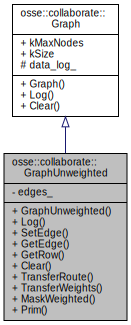
\includegraphics[width=203pt]{classosse_1_1collaborate_1_1_graph_unweighted__inherit__graph}
\end{center}
\end{figure}
\subsubsection*{Public Member Functions}
\begin{DoxyCompactItemize}
\item 
\hyperlink{classosse_1_1collaborate_1_1_graph_unweighted_a5b5c79a90fa8a8957f98e0dc4f5bafb6}{Graph\+Unweighted} (\hyperlink{classosse_1_1collaborate_1_1_data_logger}{Data\+Logger} $\ast$\+\_\+data\+\_\+log)
\begin{DoxyCompactList}\small\item\em Constructor. \end{DoxyCompactList}\item 
void \hyperlink{classosse_1_1collaborate_1_1_graph_unweighted_a06fa72fc5e51142a242fdf535af96078}{Log} (const uint16\+\_\+t \&\+\_\+num\+\_\+nodes, const uint64\+\_\+t \&\+\_\+tick) const
\begin{DoxyCompactList}\small\item\em Writes unweighted graph to a binary file. \end{DoxyCompactList}\item 
void \hyperlink{classosse_1_1collaborate_1_1_graph_unweighted_ae118a5f9c0bc24858192d13cac995f76}{Set\+Edge} (const uint16\+\_\+t \&\+\_\+row, const uint16\+\_\+t \&\+\_\+col, const bool \&\+\_\+value)
\begin{DoxyCompactList}\small\item\em Sets the edge at a row and a column to. \end{DoxyCompactList}\item 
bool \hyperlink{classosse_1_1collaborate_1_1_graph_unweighted_a60c3d775df67e19dbc49134b629c750d}{Get\+Edge} (const uint16\+\_\+t \&\+\_\+row, const uint16\+\_\+t \&\+\_\+col) const
\begin{DoxyCompactList}\small\item\em Gets the edge at a row and a column to. \end{DoxyCompactList}\item 
std\+::set$<$ uint16\+\_\+t $>$ \hyperlink{classosse_1_1collaborate_1_1_graph_unweighted_a7f648d33e2f67f09cd45395c4f8f736f}{Get\+Row} (const uint16\+\_\+t \&\+\_\+row, const uint16\+\_\+t \&\+\_\+num\+\_\+nodes) const
\begin{DoxyCompactList}\small\item\em Gets an entire row from the graph. \end{DoxyCompactList}\item 
\mbox{\Hypertarget{classosse_1_1collaborate_1_1_graph_unweighted_a9fe20052aa221d26ecd27db25c0c9391}\label{classosse_1_1collaborate_1_1_graph_unweighted_a9fe20052aa221d26ecd27db25c0c9391}} 
void \hyperlink{classosse_1_1collaborate_1_1_graph_unweighted_a9fe20052aa221d26ecd27db25c0c9391}{Clear} ()
\begin{DoxyCompactList}\small\item\em Sets all edges to false. \end{DoxyCompactList}\item 
void \hyperlink{classosse_1_1collaborate_1_1_graph_unweighted_ab38de4495671d90fe49aae2b5be2500b}{Transfer\+Route} (const std\+::vector$<$ uint16\+\_\+t $>$ \&\+\_\+route)
\begin{DoxyCompactList}\small\item\em The route is copied into the graph. \end{DoxyCompactList}\item 
void \hyperlink{classosse_1_1collaborate_1_1_graph_unweighted_ada77cbd0724afefdb49d381d63fdda24}{Transfer\+Weights} (const \hyperlink{classosse_1_1collaborate_1_1_graph_weighted}{Graph\+Weighted} \&\+\_\+weighted\+\_\+graph, const uint16\+\_\+t \&\+\_\+num\+\_\+nodes)
\begin{DoxyCompactList}\small\item\em Edges with weights are true and edges without are false. \end{DoxyCompactList}\item 
void \hyperlink{classosse_1_1collaborate_1_1_graph_unweighted_aaaffd6846abfa88f54eaa10fd24dd571}{Mask\+Weighted} (const uint16\+\_\+t \&\+\_\+num\+\_\+nodes, \hyperlink{classosse_1_1collaborate_1_1_graph_weighted}{Graph\+Weighted} $\ast$\+\_\+weighted\+\_\+graph)
\begin{DoxyCompactList}\small\item\em Mask the edges of a weighted graph. \end{DoxyCompactList}\item 
bool \hyperlink{classosse_1_1collaborate_1_1_graph_unweighted_aa64af5c58b4f322987f9d01f13c6e2d5}{Prim} (const \hyperlink{classosse_1_1collaborate_1_1_graph_weighted}{Graph\+Weighted} \&\+\_\+weighted, const uint16\+\_\+t \&\+\_\+num\+\_\+nodes)
\begin{DoxyCompactList}\small\item\em Uses Prim\textquotesingle{}s algorithm to find the minimum spanning tree in a graph. \end{DoxyCompactList}\end{DoxyCompactItemize}
\subsubsection*{Private Types}
\begin{DoxyCompactItemize}
\item 
\mbox{\Hypertarget{classosse_1_1collaborate_1_1_graph_unweighted_a218e4872b092090509bc2483186de31a}\label{classosse_1_1collaborate_1_1_graph_unweighted_a218e4872b092090509bc2483186de31a}} 
typedef std\+::array$<$ bool, \hyperlink{classosse_1_1collaborate_1_1_graph_a9c9828305d419d29fc1eed87a4520cd5}{Graph\+::k\+Size} $>$ \hyperlink{classosse_1_1collaborate_1_1_graph_unweighted_a218e4872b092090509bc2483186de31a}{Edges}
\begin{DoxyCompactList}\small\item\em Underlying adjacency attitude\+\_\+matrix. \end{DoxyCompactList}\end{DoxyCompactItemize}
\subsubsection*{Private Attributes}
\begin{DoxyCompactItemize}
\item 
\mbox{\Hypertarget{classosse_1_1collaborate_1_1_graph_unweighted_ae1e5841b64a17371fbbf2dfffe396b45}\label{classosse_1_1collaborate_1_1_graph_unweighted_ae1e5841b64a17371fbbf2dfffe396b45}} 
std\+::unique\+\_\+ptr$<$ \hyperlink{classosse_1_1collaborate_1_1_graph_unweighted_a218e4872b092090509bc2483186de31a}{Edges} $>$ \hyperlink{classosse_1_1collaborate_1_1_graph_unweighted_ae1e5841b64a17371fbbf2dfffe396b45}{edges\+\_\+}
\begin{DoxyCompactList}\small\item\em Unweighted edges. \end{DoxyCompactList}\end{DoxyCompactItemize}
\subsubsection*{Additional Inherited Members}


\subsubsection{Detailed Description}
Concrete graph with unweighted edges. 

 
\begin{DoxyImageNoCaption}
  \mbox{\includegraphics[width=\textwidth]{prim}}
\end{DoxyImageNoCaption}


\[ n_x n_x \in \{True,False\} \] \[ {\bf{E}} = Unweighted~Edges = \begin{bmatrix} 0 & n_0 n_1 & \dots & n_0 n_{N-1} & n_0 n_N \\ n_1 n_0 & 0 & \dots & n_1 n_{N-1} & n_1 n_N \\ \vdots & \vdots & \ddots & \vdots & \vdots \\ n_{N-1} n_0 & n_{N-1} n_1 & \dots & 0 & n_{N-1} n_N \\ n_N n_0 & n_N n_1 & \dots & n_N n_{N-1} & 0 \end{bmatrix} \] 

\subsubsection{Constructor \& Destructor Documentation}
\mbox{\Hypertarget{classosse_1_1collaborate_1_1_graph_unweighted_a5b5c79a90fa8a8957f98e0dc4f5bafb6}\label{classosse_1_1collaborate_1_1_graph_unweighted_a5b5c79a90fa8a8957f98e0dc4f5bafb6}} 
\index{osse\+::collaborate\+::\+Graph\+Unweighted@{osse\+::collaborate\+::\+Graph\+Unweighted}!Graph\+Unweighted@{Graph\+Unweighted}}
\index{Graph\+Unweighted@{Graph\+Unweighted}!osse\+::collaborate\+::\+Graph\+Unweighted@{osse\+::collaborate\+::\+Graph\+Unweighted}}
\paragraph{\texorpdfstring{Graph\+Unweighted()}{GraphUnweighted()}}
{\footnotesize\ttfamily osse\+::collaborate\+::\+Graph\+Unweighted\+::\+Graph\+Unweighted (\begin{DoxyParamCaption}\item[{\hyperlink{classosse_1_1collaborate_1_1_data_logger}{Data\+Logger} $\ast$}]{\+\_\+data\+\_\+log }\end{DoxyParamCaption})\hspace{0.3cm}{\ttfamily [explicit]}}



Constructor. 


\begin{DoxyParams}[1]{Parameters}
\mbox{\tt in}  & {\em \+\_\+data\+\_\+log} & Data logger \\
\hline
\end{DoxyParams}


\subsubsection{Member Function Documentation}
\mbox{\Hypertarget{classosse_1_1collaborate_1_1_graph_unweighted_a60c3d775df67e19dbc49134b629c750d}\label{classosse_1_1collaborate_1_1_graph_unweighted_a60c3d775df67e19dbc49134b629c750d}} 
\index{osse\+::collaborate\+::\+Graph\+Unweighted@{osse\+::collaborate\+::\+Graph\+Unweighted}!Get\+Edge@{Get\+Edge}}
\index{Get\+Edge@{Get\+Edge}!osse\+::collaborate\+::\+Graph\+Unweighted@{osse\+::collaborate\+::\+Graph\+Unweighted}}
\paragraph{\texorpdfstring{Get\+Edge()}{GetEdge()}}
{\footnotesize\ttfamily bool osse\+::collaborate\+::\+Graph\+Unweighted\+::\+Get\+Edge (\begin{DoxyParamCaption}\item[{const uint16\+\_\+t \&}]{\+\_\+row,  }\item[{const uint16\+\_\+t \&}]{\+\_\+col }\end{DoxyParamCaption}) const}



Gets the edge at a row and a column to. 


\begin{DoxyParams}[1]{Parameters}
\mbox{\tt in}  & {\em \+\_\+row} & Row \\
\hline
\mbox{\tt in}  & {\em \+\_\+col} & Column \\
\hline
\end{DoxyParams}
\begin{DoxyReturn}{Returns}
Value 
\end{DoxyReturn}
\mbox{\Hypertarget{classosse_1_1collaborate_1_1_graph_unweighted_a7f648d33e2f67f09cd45395c4f8f736f}\label{classosse_1_1collaborate_1_1_graph_unweighted_a7f648d33e2f67f09cd45395c4f8f736f}} 
\index{osse\+::collaborate\+::\+Graph\+Unweighted@{osse\+::collaborate\+::\+Graph\+Unweighted}!Get\+Row@{Get\+Row}}
\index{Get\+Row@{Get\+Row}!osse\+::collaborate\+::\+Graph\+Unweighted@{osse\+::collaborate\+::\+Graph\+Unweighted}}
\paragraph{\texorpdfstring{Get\+Row()}{GetRow()}}
{\footnotesize\ttfamily std\+::set$<$ uint16\+\_\+t $>$ osse\+::collaborate\+::\+Graph\+Unweighted\+::\+Get\+Row (\begin{DoxyParamCaption}\item[{const uint16\+\_\+t \&}]{\+\_\+row,  }\item[{const uint16\+\_\+t \&}]{\+\_\+num\+\_\+nodes }\end{DoxyParamCaption}) const}



Gets an entire row from the graph. 


\begin{DoxyParams}[1]{Parameters}
\mbox{\tt in}  & {\em \+\_\+row} & Row number \\
\hline
\mbox{\tt in}  & {\em \+\_\+num\+\_\+nodes} & Number of nodes \\
\hline
\end{DoxyParams}
\begin{DoxyReturn}{Returns}
Set of transmitters 
\end{DoxyReturn}
\mbox{\Hypertarget{classosse_1_1collaborate_1_1_graph_unweighted_a06fa72fc5e51142a242fdf535af96078}\label{classosse_1_1collaborate_1_1_graph_unweighted_a06fa72fc5e51142a242fdf535af96078}} 
\index{osse\+::collaborate\+::\+Graph\+Unweighted@{osse\+::collaborate\+::\+Graph\+Unweighted}!Log@{Log}}
\index{Log@{Log}!osse\+::collaborate\+::\+Graph\+Unweighted@{osse\+::collaborate\+::\+Graph\+Unweighted}}
\paragraph{\texorpdfstring{Log()}{Log()}}
{\footnotesize\ttfamily void osse\+::collaborate\+::\+Graph\+Unweighted\+::\+Log (\begin{DoxyParamCaption}\item[{const uint16\+\_\+t \&}]{\+\_\+num\+\_\+nodes,  }\item[{const uint64\+\_\+t \&}]{\+\_\+tick }\end{DoxyParamCaption}) const\hspace{0.3cm}{\ttfamily [virtual]}}



Writes unweighted graph to a binary file. 


\begin{DoxyParams}[1]{Parameters}
\mbox{\tt in}  & {\em \+\_\+num\+\_\+nodes} & Number of nodes (rows and columns) \\
\hline
\mbox{\tt in}  & {\em \+\_\+tick} & The simulation clock tick \\
\hline
\end{DoxyParams}


Implements \hyperlink{classosse_1_1collaborate_1_1_graph_abaef7c4642242e096d2bbfc74b8d1d07}{osse\+::collaborate\+::\+Graph}.

\mbox{\Hypertarget{classosse_1_1collaborate_1_1_graph_unweighted_aaaffd6846abfa88f54eaa10fd24dd571}\label{classosse_1_1collaborate_1_1_graph_unweighted_aaaffd6846abfa88f54eaa10fd24dd571}} 
\index{osse\+::collaborate\+::\+Graph\+Unweighted@{osse\+::collaborate\+::\+Graph\+Unweighted}!Mask\+Weighted@{Mask\+Weighted}}
\index{Mask\+Weighted@{Mask\+Weighted}!osse\+::collaborate\+::\+Graph\+Unweighted@{osse\+::collaborate\+::\+Graph\+Unweighted}}
\paragraph{\texorpdfstring{Mask\+Weighted()}{MaskWeighted()}}
{\footnotesize\ttfamily void osse\+::collaborate\+::\+Graph\+Unweighted\+::\+Mask\+Weighted (\begin{DoxyParamCaption}\item[{const uint16\+\_\+t \&}]{\+\_\+num\+\_\+nodes,  }\item[{\hyperlink{classosse_1_1collaborate_1_1_graph_weighted}{Graph\+Weighted} $\ast$}]{\+\_\+weighted\+\_\+graph }\end{DoxyParamCaption})}



Mask the edges of a weighted graph. 


\begin{DoxyParams}[1]{Parameters}
\mbox{\tt in}  & {\em \+\_\+weighted\+\_\+graph} & Weighted graph \\
\hline
\mbox{\tt in}  & {\em \+\_\+num\+\_\+nodes} & Number of nodes \\
\hline
\end{DoxyParams}
\mbox{\Hypertarget{classosse_1_1collaborate_1_1_graph_unweighted_aa64af5c58b4f322987f9d01f13c6e2d5}\label{classosse_1_1collaborate_1_1_graph_unweighted_aa64af5c58b4f322987f9d01f13c6e2d5}} 
\index{osse\+::collaborate\+::\+Graph\+Unweighted@{osse\+::collaborate\+::\+Graph\+Unweighted}!Prim@{Prim}}
\index{Prim@{Prim}!osse\+::collaborate\+::\+Graph\+Unweighted@{osse\+::collaborate\+::\+Graph\+Unweighted}}
\paragraph{\texorpdfstring{Prim()}{Prim()}}
{\footnotesize\ttfamily bool osse\+::collaborate\+::\+Graph\+Unweighted\+::\+Prim (\begin{DoxyParamCaption}\item[{const \hyperlink{classosse_1_1collaborate_1_1_graph_weighted}{Graph\+Weighted} \&}]{\+\_\+weighted,  }\item[{const uint16\+\_\+t \&}]{\+\_\+num\+\_\+nodes }\end{DoxyParamCaption})}



Uses Prim\textquotesingle{}s algorithm to find the minimum spanning tree in a graph. 


\begin{DoxyParams}[1]{Parameters}
\mbox{\tt in}  & {\em \+\_\+weighted} & Weighted graph \\
\hline
\end{DoxyParams}
\begin{DoxyReturn}{Returns}
connected\+\_\+ Whether or not the graph is connected 
\end{DoxyReturn}

\begin{DoxyParams}[1]{Parameters}
\mbox{\tt in}  & {\em \+\_\+num\+\_\+nodes} & Number of nodes (rows and columns) \\
\hline
\end{DoxyParams}
\mbox{\Hypertarget{classosse_1_1collaborate_1_1_graph_unweighted_ae118a5f9c0bc24858192d13cac995f76}\label{classosse_1_1collaborate_1_1_graph_unweighted_ae118a5f9c0bc24858192d13cac995f76}} 
\index{osse\+::collaborate\+::\+Graph\+Unweighted@{osse\+::collaborate\+::\+Graph\+Unweighted}!Set\+Edge@{Set\+Edge}}
\index{Set\+Edge@{Set\+Edge}!osse\+::collaborate\+::\+Graph\+Unweighted@{osse\+::collaborate\+::\+Graph\+Unweighted}}
\paragraph{\texorpdfstring{Set\+Edge()}{SetEdge()}}
{\footnotesize\ttfamily void osse\+::collaborate\+::\+Graph\+Unweighted\+::\+Set\+Edge (\begin{DoxyParamCaption}\item[{const uint16\+\_\+t \&}]{\+\_\+row,  }\item[{const uint16\+\_\+t \&}]{\+\_\+col,  }\item[{const bool \&}]{\+\_\+value }\end{DoxyParamCaption})}



Sets the edge at a row and a column to. 


\begin{DoxyParams}[1]{Parameters}
\mbox{\tt in}  & {\em \+\_\+row} & Row \\
\hline
\mbox{\tt in}  & {\em \+\_\+col} & Column \\
\hline
\mbox{\tt in}  & {\em \+\_\+value} & Value \\
\hline
\end{DoxyParams}
\mbox{\Hypertarget{classosse_1_1collaborate_1_1_graph_unweighted_ab38de4495671d90fe49aae2b5be2500b}\label{classosse_1_1collaborate_1_1_graph_unweighted_ab38de4495671d90fe49aae2b5be2500b}} 
\index{osse\+::collaborate\+::\+Graph\+Unweighted@{osse\+::collaborate\+::\+Graph\+Unweighted}!Transfer\+Route@{Transfer\+Route}}
\index{Transfer\+Route@{Transfer\+Route}!osse\+::collaborate\+::\+Graph\+Unweighted@{osse\+::collaborate\+::\+Graph\+Unweighted}}
\paragraph{\texorpdfstring{Transfer\+Route()}{TransferRoute()}}
{\footnotesize\ttfamily void osse\+::collaborate\+::\+Graph\+Unweighted\+::\+Transfer\+Route (\begin{DoxyParamCaption}\item[{const std\+::vector$<$ uint16\+\_\+t $>$ \&}]{\+\_\+route }\end{DoxyParamCaption})}



The route is copied into the graph. 


\begin{DoxyParams}[1]{Parameters}
\mbox{\tt in}  & {\em \+\_\+route} & Route \\
\hline
\end{DoxyParams}
\mbox{\Hypertarget{classosse_1_1collaborate_1_1_graph_unweighted_ada77cbd0724afefdb49d381d63fdda24}\label{classosse_1_1collaborate_1_1_graph_unweighted_ada77cbd0724afefdb49d381d63fdda24}} 
\index{osse\+::collaborate\+::\+Graph\+Unweighted@{osse\+::collaborate\+::\+Graph\+Unweighted}!Transfer\+Weights@{Transfer\+Weights}}
\index{Transfer\+Weights@{Transfer\+Weights}!osse\+::collaborate\+::\+Graph\+Unweighted@{osse\+::collaborate\+::\+Graph\+Unweighted}}
\paragraph{\texorpdfstring{Transfer\+Weights()}{TransferWeights()}}
{\footnotesize\ttfamily void osse\+::collaborate\+::\+Graph\+Unweighted\+::\+Transfer\+Weights (\begin{DoxyParamCaption}\item[{const \hyperlink{classosse_1_1collaborate_1_1_graph_weighted}{Graph\+Weighted} \&}]{\+\_\+weighted\+\_\+graph,  }\item[{const uint16\+\_\+t \&}]{\+\_\+num\+\_\+nodes }\end{DoxyParamCaption})}



Edges with weights are true and edges without are false. 


\begin{DoxyParams}[1]{Parameters}
\mbox{\tt in}  & {\em \+\_\+weighted\+\_\+graph} & Weighted graph \\
\hline
\mbox{\tt in}  & {\em \+\_\+num\+\_\+nodes} & Number of nodes \\
\hline
\end{DoxyParams}


The documentation for this class was generated from the following files\+:\begin{DoxyCompactItemize}
\item 
libs/collaborate/include/collaborate/graph\+\_\+unweighted.\+h\item 
libs/collaborate/src/graph\+\_\+unweighted.\+cpp\end{DoxyCompactItemize}

\hypertarget{classosse_1_1collaborate_1_1_graph_weighted}{}\subsection{osse\+:\+:collaborate\+:\+:Graph\+Weighted Class Reference}
\label{classosse_1_1collaborate_1_1_graph_weighted}\index{osse\+::collaborate\+::\+Graph\+Weighted@{osse\+::collaborate\+::\+Graph\+Weighted}}


Concrete graph with weighted edges.  




{\ttfamily \#include $<$graph\+\_\+weighted.\+h$>$}



Inheritance diagram for osse\+:\+:collaborate\+:\+:Graph\+Weighted\+:
\nopagebreak
\begin{figure}[H]
\begin{center}
\leavevmode
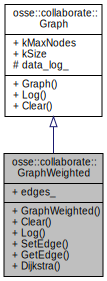
\includegraphics[width=190pt]{classosse_1_1collaborate_1_1_graph_weighted__inherit__graph}
\end{center}
\end{figure}
\subsubsection*{Public Types}
\begin{DoxyCompactItemize}
\item 
\mbox{\Hypertarget{classosse_1_1collaborate_1_1_graph_weighted_aa604a648e701d85c8deb818f13b64097}\label{classosse_1_1collaborate_1_1_graph_weighted_aa604a648e701d85c8deb818f13b64097}} 
typedef std\+::array$<$ double, \hyperlink{classosse_1_1collaborate_1_1_graph_a9c9828305d419d29fc1eed87a4520cd5}{Graph\+::k\+Size} $>$ \hyperlink{classosse_1_1collaborate_1_1_graph_weighted_aa604a648e701d85c8deb818f13b64097}{Edges}
\begin{DoxyCompactList}\small\item\em Underlying adjacency attitude\+\_\+matrix. \end{DoxyCompactList}\end{DoxyCompactItemize}
\subsubsection*{Public Member Functions}
\begin{DoxyCompactItemize}
\item 
\hyperlink{classosse_1_1collaborate_1_1_graph_weighted_a983e8d0efd6bba488b979b546cb078ff}{Graph\+Weighted} (\hyperlink{classosse_1_1collaborate_1_1_data_logger}{Data\+Logger} $\ast$\+\_\+data\+\_\+log)
\begin{DoxyCompactList}\small\item\em Constructor. \end{DoxyCompactList}\item 
\mbox{\Hypertarget{classosse_1_1collaborate_1_1_graph_weighted_a485197f02e24b37e2e2e47136548aa3d}\label{classosse_1_1collaborate_1_1_graph_weighted_a485197f02e24b37e2e2e47136548aa3d}} 
void \hyperlink{classosse_1_1collaborate_1_1_graph_weighted_a485197f02e24b37e2e2e47136548aa3d}{Clear} ()
\begin{DoxyCompactList}\small\item\em Sets all edges to 0.\+0. \end{DoxyCompactList}\item 
void \hyperlink{classosse_1_1collaborate_1_1_graph_weighted_ab55668685b7bde8d3553cedeb95efab3}{Log} (const uint16\+\_\+t \&\+\_\+num\+\_\+nodes, const uint64\+\_\+t \&\+\_\+tick) const
\begin{DoxyCompactList}\small\item\em Writes the weighted graph to a binary file. \end{DoxyCompactList}\item 
void \hyperlink{classosse_1_1collaborate_1_1_graph_weighted_a20ad6c253cec6b39d5d2cee4aa5ea073}{Set\+Edge} (const uint16\+\_\+t \&\+\_\+row, const uint16\+\_\+t \&\+\_\+col, const double \&\+\_\+value)
\begin{DoxyCompactList}\small\item\em Sets the edge at a row and a column to. \end{DoxyCompactList}\item 
double \hyperlink{classosse_1_1collaborate_1_1_graph_weighted_a10d1d7bb90d63fa8461e044ca5b2bd20}{Get\+Edge} (const uint16\+\_\+t \&\+\_\+row, const uint16\+\_\+t \&\+\_\+col) const
\begin{DoxyCompactList}\small\item\em Gets the edge at a row and a column to. \end{DoxyCompactList}\item 
std\+::vector$<$ uint16\+\_\+t $>$ \hyperlink{classosse_1_1collaborate_1_1_graph_weighted_a657a68399222496d6664418061fe2108}{Dijkstra} (const uint16\+\_\+t \&\+\_\+start, const uint16\+\_\+t \&\+\_\+end)
\begin{DoxyCompactList}\small\item\em Uses Dijkstra\textquotesingle{}s algorithm to find shortest path between two nodes. \end{DoxyCompactList}\end{DoxyCompactItemize}
\subsubsection*{Data Fields}
\begin{DoxyCompactItemize}
\item 
\mbox{\Hypertarget{classosse_1_1collaborate_1_1_graph_weighted_a60944e002d7910e9de5d2bba3ea87e74}\label{classosse_1_1collaborate_1_1_graph_weighted_a60944e002d7910e9de5d2bba3ea87e74}} 
std\+::unique\+\_\+ptr$<$ \hyperlink{classosse_1_1collaborate_1_1_graph_weighted_aa604a648e701d85c8deb818f13b64097}{Edges} $>$ \hyperlink{classosse_1_1collaborate_1_1_graph_weighted_a60944e002d7910e9de5d2bba3ea87e74}{edges\+\_\+}
\begin{DoxyCompactList}\small\item\em Weighted edges. \end{DoxyCompactList}\end{DoxyCompactItemize}
\subsubsection*{Additional Inherited Members}


\subsubsection{Detailed Description}
Concrete graph with weighted edges. 

 
\begin{DoxyImageNoCaption}
  \mbox{\includegraphics[width=\textwidth]{weighted}}
\end{DoxyImageNoCaption}


\[ n_x n_x \in \mathbb{R} \] \[ {\bf{E}} = Weighted~Edges = \begin{bmatrix} 0 & n_0 n_1 & \dots & n_0 n_{N-1} & n_0 n_N \\ n_1 n_0 & 0 & \dots & n_1 n_{N-1} & n_1 n_N \\ \vdots & \vdots & \ddots & \vdots & \vdots \\ n_{N-1} n_0 & n_{N-1} n_1 & \dots & 0 & n_{N-1} n_N \\ n_N n_0 & n_N n_1 & \dots & n_N n_{N-1} & 0 \end{bmatrix} \] 

\subsubsection{Constructor \& Destructor Documentation}
\mbox{\Hypertarget{classosse_1_1collaborate_1_1_graph_weighted_a983e8d0efd6bba488b979b546cb078ff}\label{classosse_1_1collaborate_1_1_graph_weighted_a983e8d0efd6bba488b979b546cb078ff}} 
\index{osse\+::collaborate\+::\+Graph\+Weighted@{osse\+::collaborate\+::\+Graph\+Weighted}!Graph\+Weighted@{Graph\+Weighted}}
\index{Graph\+Weighted@{Graph\+Weighted}!osse\+::collaborate\+::\+Graph\+Weighted@{osse\+::collaborate\+::\+Graph\+Weighted}}
\paragraph{\texorpdfstring{Graph\+Weighted()}{GraphWeighted()}}
{\footnotesize\ttfamily osse\+::collaborate\+::\+Graph\+Weighted\+::\+Graph\+Weighted (\begin{DoxyParamCaption}\item[{\hyperlink{classosse_1_1collaborate_1_1_data_logger}{Data\+Logger} $\ast$}]{\+\_\+data\+\_\+log }\end{DoxyParamCaption})\hspace{0.3cm}{\ttfamily [explicit]}}



Constructor. 


\begin{DoxyParams}[1]{Parameters}
\mbox{\tt in}  & {\em \+\_\+data\+\_\+log} & Data logger \\
\hline
\end{DoxyParams}


\subsubsection{Member Function Documentation}
\mbox{\Hypertarget{classosse_1_1collaborate_1_1_graph_weighted_a657a68399222496d6664418061fe2108}\label{classosse_1_1collaborate_1_1_graph_weighted_a657a68399222496d6664418061fe2108}} 
\index{osse\+::collaborate\+::\+Graph\+Weighted@{osse\+::collaborate\+::\+Graph\+Weighted}!Dijkstra@{Dijkstra}}
\index{Dijkstra@{Dijkstra}!osse\+::collaborate\+::\+Graph\+Weighted@{osse\+::collaborate\+::\+Graph\+Weighted}}
\paragraph{\texorpdfstring{Dijkstra()}{Dijkstra()}}
{\footnotesize\ttfamily std\+::vector$<$ uint16\+\_\+t $>$ osse\+::collaborate\+::\+Graph\+Weighted\+::\+Dijkstra (\begin{DoxyParamCaption}\item[{const uint16\+\_\+t \&}]{\+\_\+start,  }\item[{const uint16\+\_\+t \&}]{\+\_\+end }\end{DoxyParamCaption})}



Uses Dijkstra\textquotesingle{}s algorithm to find shortest path between two nodes. 


\begin{DoxyParams}[1]{Parameters}
\mbox{\tt in}  & {\em \+\_\+start} & Beginning index \\
\hline
\mbox{\tt in}  & {\em \+\_\+end} & End index \\
\hline
\end{DoxyParams}
\begin{DoxyReturn}{Returns}
Shortest path between the nodes 
\end{DoxyReturn}
\mbox{\Hypertarget{classosse_1_1collaborate_1_1_graph_weighted_a10d1d7bb90d63fa8461e044ca5b2bd20}\label{classosse_1_1collaborate_1_1_graph_weighted_a10d1d7bb90d63fa8461e044ca5b2bd20}} 
\index{osse\+::collaborate\+::\+Graph\+Weighted@{osse\+::collaborate\+::\+Graph\+Weighted}!Get\+Edge@{Get\+Edge}}
\index{Get\+Edge@{Get\+Edge}!osse\+::collaborate\+::\+Graph\+Weighted@{osse\+::collaborate\+::\+Graph\+Weighted}}
\paragraph{\texorpdfstring{Get\+Edge()}{GetEdge()}}
{\footnotesize\ttfamily double osse\+::collaborate\+::\+Graph\+Weighted\+::\+Get\+Edge (\begin{DoxyParamCaption}\item[{const uint16\+\_\+t \&}]{\+\_\+row,  }\item[{const uint16\+\_\+t \&}]{\+\_\+col }\end{DoxyParamCaption}) const}



Gets the edge at a row and a column to. 


\begin{DoxyParams}[1]{Parameters}
\mbox{\tt in}  & {\em \+\_\+row} & Row \\
\hline
\mbox{\tt in}  & {\em \+\_\+col} & Column \\
\hline
\end{DoxyParams}
\begin{DoxyReturn}{Returns}
Value 
\end{DoxyReturn}
\mbox{\Hypertarget{classosse_1_1collaborate_1_1_graph_weighted_ab55668685b7bde8d3553cedeb95efab3}\label{classosse_1_1collaborate_1_1_graph_weighted_ab55668685b7bde8d3553cedeb95efab3}} 
\index{osse\+::collaborate\+::\+Graph\+Weighted@{osse\+::collaborate\+::\+Graph\+Weighted}!Log@{Log}}
\index{Log@{Log}!osse\+::collaborate\+::\+Graph\+Weighted@{osse\+::collaborate\+::\+Graph\+Weighted}}
\paragraph{\texorpdfstring{Log()}{Log()}}
{\footnotesize\ttfamily void osse\+::collaborate\+::\+Graph\+Weighted\+::\+Log (\begin{DoxyParamCaption}\item[{const uint16\+\_\+t \&}]{\+\_\+num\+\_\+nodes,  }\item[{const uint64\+\_\+t \&}]{\+\_\+tick }\end{DoxyParamCaption}) const\hspace{0.3cm}{\ttfamily [virtual]}}



Writes the weighted graph to a binary file. 


\begin{DoxyParams}[1]{Parameters}
\mbox{\tt in}  & {\em \+\_\+num\+\_\+nodes} & Number of nodes (rows and columns) \\
\hline
\mbox{\tt in}  & {\em \+\_\+tick} & The simulation clock tick \\
\hline
\end{DoxyParams}


Implements \hyperlink{classosse_1_1collaborate_1_1_graph_abaef7c4642242e096d2bbfc74b8d1d07}{osse\+::collaborate\+::\+Graph}.

\mbox{\Hypertarget{classosse_1_1collaborate_1_1_graph_weighted_a20ad6c253cec6b39d5d2cee4aa5ea073}\label{classosse_1_1collaborate_1_1_graph_weighted_a20ad6c253cec6b39d5d2cee4aa5ea073}} 
\index{osse\+::collaborate\+::\+Graph\+Weighted@{osse\+::collaborate\+::\+Graph\+Weighted}!Set\+Edge@{Set\+Edge}}
\index{Set\+Edge@{Set\+Edge}!osse\+::collaborate\+::\+Graph\+Weighted@{osse\+::collaborate\+::\+Graph\+Weighted}}
\paragraph{\texorpdfstring{Set\+Edge()}{SetEdge()}}
{\footnotesize\ttfamily void osse\+::collaborate\+::\+Graph\+Weighted\+::\+Set\+Edge (\begin{DoxyParamCaption}\item[{const uint16\+\_\+t \&}]{\+\_\+row,  }\item[{const uint16\+\_\+t \&}]{\+\_\+col,  }\item[{const double \&}]{\+\_\+value }\end{DoxyParamCaption})}



Sets the edge at a row and a column to. 


\begin{DoxyParams}[1]{Parameters}
\mbox{\tt in}  & {\em \+\_\+row} & Row \\
\hline
\mbox{\tt in}  & {\em \+\_\+col} & Column \\
\hline
\mbox{\tt in}  & {\em \+\_\+value} & Value \\
\hline
\end{DoxyParams}


The documentation for this class was generated from the following files\+:\begin{DoxyCompactItemize}
\item 
libs/collaborate/include/collaborate/graph\+\_\+weighted.\+h\item 
libs/collaborate/src/graph\+\_\+weighted.\+cpp\end{DoxyCompactItemize}

\hypertarget{classosse_1_1collaborate_1_1_graph}{}\subsection{osse\+:\+:collaborate\+:\+:Graph Class Reference}
\label{classosse_1_1collaborate_1_1_graph}\index{osse\+::collaborate\+::\+Graph@{osse\+::collaborate\+::\+Graph}}


Abstract graph.  




{\ttfamily \#include $<$graph.\+h$>$}



Inheritance diagram for osse\+:\+:collaborate\+:\+:Graph\+:
\nopagebreak
\begin{figure}[H]
\begin{center}
\leavevmode
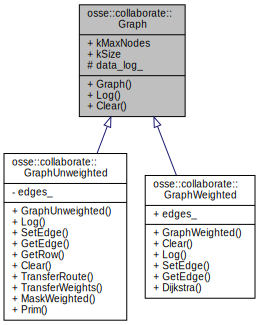
\includegraphics[width=332pt]{classosse_1_1collaborate_1_1_graph__inherit__graph}
\end{center}
\end{figure}
\subsubsection*{Public Member Functions}
\begin{DoxyCompactItemize}
\item 
\hyperlink{classosse_1_1collaborate_1_1_graph_aa6e69d08b74393ecfa68cbf915d7eabc}{Graph} (\hyperlink{classosse_1_1collaborate_1_1_data_logger}{Data\+Logger} $\ast$\+\_\+data\+\_\+log)
\begin{DoxyCompactList}\small\item\em Constructor. \end{DoxyCompactList}\item 
virtual void \hyperlink{classosse_1_1collaborate_1_1_graph_abaef7c4642242e096d2bbfc74b8d1d07}{Log} (const uint16\+\_\+t \&\+\_\+num\+\_\+nodes, const uint64\+\_\+t \&\+\_\+tick) const =0
\begin{DoxyCompactList}\small\item\em Writes graph to a binary file. \end{DoxyCompactList}\item 
\mbox{\Hypertarget{classosse_1_1collaborate_1_1_graph_a92b99db1a453e58d1fb3fc134a8fd8ba}\label{classosse_1_1collaborate_1_1_graph_a92b99db1a453e58d1fb3fc134a8fd8ba}} 
virtual void \hyperlink{classosse_1_1collaborate_1_1_graph_a92b99db1a453e58d1fb3fc134a8fd8ba}{Clear} ()=0
\begin{DoxyCompactList}\small\item\em Clears all edges. \end{DoxyCompactList}\end{DoxyCompactItemize}
\subsubsection*{Static Public Attributes}
\begin{DoxyCompactItemize}
\item 
\mbox{\Hypertarget{classosse_1_1collaborate_1_1_graph_a063285c7a14ce7499b355cac87d1900a}\label{classosse_1_1collaborate_1_1_graph_a063285c7a14ce7499b355cac87d1900a}} 
static constexpr uint16\+\_\+t \hyperlink{classosse_1_1collaborate_1_1_graph_a063285c7a14ce7499b355cac87d1900a}{k\+Max\+Nodes} = 200
\begin{DoxyCompactList}\small\item\em Maximum number of nodes. \end{DoxyCompactList}\item 
\mbox{\Hypertarget{classosse_1_1collaborate_1_1_graph_a9c9828305d419d29fc1eed87a4520cd5}\label{classosse_1_1collaborate_1_1_graph_a9c9828305d419d29fc1eed87a4520cd5}} 
static constexpr uint16\+\_\+t \hyperlink{classosse_1_1collaborate_1_1_graph_a9c9828305d419d29fc1eed87a4520cd5}{k\+Size} = std\+::pow(\hyperlink{classosse_1_1collaborate_1_1_graph_a063285c7a14ce7499b355cac87d1900a}{k\+Max\+Nodes}, 2)
\begin{DoxyCompactList}\small\item\em Maximum size of of a graph. \end{DoxyCompactList}\end{DoxyCompactItemize}
\subsubsection*{Protected Attributes}
\begin{DoxyCompactItemize}
\item 
\mbox{\Hypertarget{classosse_1_1collaborate_1_1_graph_a33e2d89c03913f2bb033a215b5f1efa6}\label{classosse_1_1collaborate_1_1_graph_a33e2d89c03913f2bb033a215b5f1efa6}} 
\hyperlink{classosse_1_1collaborate_1_1_data_logger}{Data\+Logger} $\ast$ \hyperlink{classosse_1_1collaborate_1_1_graph_a33e2d89c03913f2bb033a215b5f1efa6}{data\+\_\+log\+\_\+}
\begin{DoxyCompactList}\small\item\em Data logger. \end{DoxyCompactList}\end{DoxyCompactItemize}


\subsubsection{Detailed Description}
Abstract graph. 

\subsubsection{Constructor \& Destructor Documentation}
\mbox{\Hypertarget{classosse_1_1collaborate_1_1_graph_aa6e69d08b74393ecfa68cbf915d7eabc}\label{classosse_1_1collaborate_1_1_graph_aa6e69d08b74393ecfa68cbf915d7eabc}} 
\index{osse\+::collaborate\+::\+Graph@{osse\+::collaborate\+::\+Graph}!Graph@{Graph}}
\index{Graph@{Graph}!osse\+::collaborate\+::\+Graph@{osse\+::collaborate\+::\+Graph}}
\paragraph{\texorpdfstring{Graph()}{Graph()}}
{\footnotesize\ttfamily osse\+::collaborate\+::\+Graph\+::\+Graph (\begin{DoxyParamCaption}\item[{\hyperlink{classosse_1_1collaborate_1_1_data_logger}{Data\+Logger} $\ast$}]{\+\_\+data\+\_\+log }\end{DoxyParamCaption})\hspace{0.3cm}{\ttfamily [explicit]}}



Constructor. 


\begin{DoxyParams}[1]{Parameters}
\mbox{\tt in}  & {\em \+\_\+data\+\_\+log} & Data logger \\
\hline
\end{DoxyParams}


\subsubsection{Member Function Documentation}
\mbox{\Hypertarget{classosse_1_1collaborate_1_1_graph_abaef7c4642242e096d2bbfc74b8d1d07}\label{classosse_1_1collaborate_1_1_graph_abaef7c4642242e096d2bbfc74b8d1d07}} 
\index{osse\+::collaborate\+::\+Graph@{osse\+::collaborate\+::\+Graph}!Log@{Log}}
\index{Log@{Log}!osse\+::collaborate\+::\+Graph@{osse\+::collaborate\+::\+Graph}}
\paragraph{\texorpdfstring{Log()}{Log()}}
{\footnotesize\ttfamily virtual void osse\+::collaborate\+::\+Graph\+::\+Log (\begin{DoxyParamCaption}\item[{const uint16\+\_\+t \&}]{\+\_\+num\+\_\+nodes,  }\item[{const uint64\+\_\+t \&}]{\+\_\+tick }\end{DoxyParamCaption}) const\hspace{0.3cm}{\ttfamily [pure virtual]}}



Writes graph to a binary file. 


\begin{DoxyParams}[1]{Parameters}
\mbox{\tt in}  & {\em \+\_\+num\+\_\+nodes} & Number of nodes (rows and columns) \\
\hline
\mbox{\tt in}  & {\em \+\_\+tick} & The simulation clock tick \\
\hline
\end{DoxyParams}


Implemented in \hyperlink{classosse_1_1collaborate_1_1_graph_weighted_ab55668685b7bde8d3553cedeb95efab3}{osse\+::collaborate\+::\+Graph\+Weighted}, and \hyperlink{classosse_1_1collaborate_1_1_graph_unweighted_a06fa72fc5e51142a242fdf535af96078}{osse\+::collaborate\+::\+Graph\+Unweighted}.



The documentation for this class was generated from the following files\+:\begin{DoxyCompactItemize}
\item 
libs/collaborate/include/collaborate/graph.\+h\item 
libs/collaborate/src/graph.\+cpp\end{DoxyCompactItemize}

\hypertarget{classosse_1_1collaborate_1_1_modem_uhf_deploy}{}\subsection{osse\+:\+:collaborate\+:\+:Modem\+Uhf\+Deploy Class Reference}
\label{classosse_1_1collaborate_1_1_modem_uhf_deploy}\index{osse\+::collaborate\+::\+Modem\+Uhf\+Deploy@{osse\+::collaborate\+::\+Modem\+Uhf\+Deploy}}


Concrete U\+HF modem (deployed on a satellite)  




{\ttfamily \#include $<$modem\+\_\+uhf\+\_\+deploy.\+h$>$}



Inheritance diagram for osse\+:\+:collaborate\+:\+:Modem\+Uhf\+Deploy\+:
\nopagebreak
\begin{figure}[H]
\begin{center}
\leavevmode
\includegraphics[width=226pt]{classosse_1_1collaborate_1_1_modem_uhf_deploy__inherit__graph}
\end{center}
\end{figure}
\subsubsection*{Public Member Functions}
\begin{DoxyCompactItemize}
\item 
\mbox{\Hypertarget{classosse_1_1collaborate_1_1_modem_uhf_deploy_a91e8e69f8a8cbaad00c874f24af2a0da}\label{classosse_1_1collaborate_1_1_modem_uhf_deploy_a91e8e69f8a8cbaad00c874f24af2a0da}} 
\hyperlink{classosse_1_1collaborate_1_1_modem_uhf_deploy_a91e8e69f8a8cbaad00c874f24af2a0da}{Modem\+Uhf\+Deploy} ()
\begin{DoxyCompactList}\small\item\em Constructor. \end{DoxyCompactList}\end{DoxyCompactItemize}
\subsubsection*{Additional Inherited Members}


\subsubsection{Detailed Description}
Concrete U\+HF modem (deployed on a satellite) 

The documentation for this class was generated from the following files\+:\begin{DoxyCompactItemize}
\item 
libs/collaborate/include/collaborate/modem\+\_\+uhf\+\_\+deploy.\+h\item 
libs/collaborate/src/modem\+\_\+uhf\+\_\+deploy.\+cpp\end{DoxyCompactItemize}

\hypertarget{classosse_1_1collaborate_1_1_modem_uhf_station}{}\subsection{osse\+:\+:collaborate\+:\+:Modem\+Uhf\+Station Class Reference}
\label{classosse_1_1collaborate_1_1_modem_uhf_station}\index{osse\+::collaborate\+::\+Modem\+Uhf\+Station@{osse\+::collaborate\+::\+Modem\+Uhf\+Station}}


Concrete U\+HF modem (base station)  




{\ttfamily \#include $<$modem\+\_\+uhf\+\_\+station.\+h$>$}



Inheritance diagram for osse\+:\+:collaborate\+:\+:Modem\+Uhf\+Station\+:
\nopagebreak
\begin{figure}[H]
\begin{center}
\leavevmode
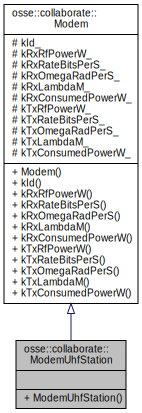
\includegraphics[width=226pt]{classosse_1_1collaborate_1_1_modem_uhf_station__inherit__graph}
\end{center}
\end{figure}
\subsubsection*{Public Member Functions}
\begin{DoxyCompactItemize}
\item 
\mbox{\Hypertarget{classosse_1_1collaborate_1_1_modem_uhf_station_a26cc4da6ecf733547178400fbfaac340}\label{classosse_1_1collaborate_1_1_modem_uhf_station_a26cc4da6ecf733547178400fbfaac340}} 
\hyperlink{classosse_1_1collaborate_1_1_modem_uhf_station_a26cc4da6ecf733547178400fbfaac340}{Modem\+Uhf\+Station} ()
\begin{DoxyCompactList}\small\item\em Constructor. \end{DoxyCompactList}\end{DoxyCompactItemize}
\subsubsection*{Additional Inherited Members}


\subsubsection{Detailed Description}
Concrete U\+HF modem (base station) 

The documentation for this class was generated from the following files\+:\begin{DoxyCompactItemize}
\item 
libs/collaborate/include/collaborate/modem\+\_\+uhf\+\_\+station.\+h\item 
libs/collaborate/src/modem\+\_\+uhf\+\_\+station.\+cpp\end{DoxyCompactItemize}

\hypertarget{classosse_1_1collaborate_1_1_modem}{}\subsection{osse\+:\+:collaborate\+:\+:Modem Class Reference}
\label{classosse_1_1collaborate_1_1_modem}\index{osse\+::collaborate\+::\+Modem@{osse\+::collaborate\+::\+Modem}}


Abstract modem.  




{\ttfamily \#include $<$modem.\+h$>$}



Inheritance diagram for osse\+:\+:collaborate\+:\+:Modem\+:
\nopagebreak
\begin{figure}[H]
\begin{center}
\leavevmode
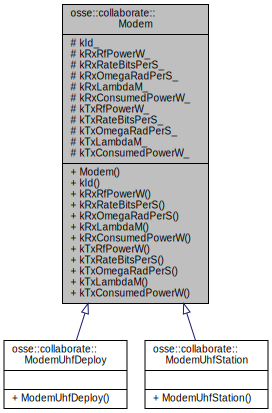
\includegraphics[width=344pt]{classosse_1_1collaborate_1_1_modem__inherit__graph}
\end{center}
\end{figure}
\subsubsection*{Public Member Functions}
\begin{DoxyCompactItemize}
\item 
\hyperlink{classosse_1_1collaborate_1_1_modem_ade030a147d5bc9aaf4a0b615c1cea84a}{Modem} (const std\+::string \&\+\_\+k\+Id, const double \&\+\_\+k\+Rx\+Rf\+PowerW, const uint64\+\_\+t \&\+\_\+k\+Rx\+Rate\+Bits\+PerS, const double \&\+\_\+k\+Rx\+Omega\+Rad\+PerS, const double \&\+\_\+k\+Rx\+LambdaM, const double \&\+\_\+k\+Rx\+Consumed\+PowerW, const double \&\+\_\+k\+Tx\+Rf\+PowerW, const uint64\+\_\+t \&\+\_\+k\+Tx\+Rate\+Bits\+PerS, const double \&\+\_\+k\+Tx\+Omega\+Rad\+PerS, const double \&\+\_\+k\+Tx\+LambdaM, const double \&\+\_\+k\+Tx\+Consumed\+PowerW)
\begin{DoxyCompactList}\small\item\em Constructor. \end{DoxyCompactList}\item 
const std\+::string \& \hyperlink{classosse_1_1collaborate_1_1_modem_a8cc084d7cc349b4029f1281c5d3248a3}{k\+Id} ()
\begin{DoxyCompactList}\small\item\em Get ID. \end{DoxyCompactList}\item 
const double \& \hyperlink{classosse_1_1collaborate_1_1_modem_ad37beed0399591a98a47b62966a7c2c0}{k\+Rx\+Rf\+PowerW} () const
\begin{DoxyCompactList}\small\item\em Get RX RF power (watts) \end{DoxyCompactList}\item 
const uint64\+\_\+t \& \hyperlink{classosse_1_1collaborate_1_1_modem_a899a9e97b55878e6b521038ddb2a9548}{k\+Rx\+Rate\+Bits\+PerS} () const
\begin{DoxyCompactList}\small\item\em Get RX data rate (bits per second) \end{DoxyCompactList}\item 
const double \& \hyperlink{classosse_1_1collaborate_1_1_modem_ac20ca2074113d6e21c8351c22f821bf2}{k\+Rx\+Omega\+Rad\+PerS} () const
\begin{DoxyCompactList}\small\item\em Get RX frequency (radians per second) \end{DoxyCompactList}\item 
const double \& \hyperlink{classosse_1_1collaborate_1_1_modem_a3e5ffe93c09f9e615d6706bcf66a5b92}{k\+Rx\+LambdaM} () const
\begin{DoxyCompactList}\small\item\em Get RX wavelength (meters) \end{DoxyCompactList}\item 
const double \& \hyperlink{classosse_1_1collaborate_1_1_modem_a1d7fde5092bef180161739258d68acc4}{k\+Rx\+Consumed\+PowerW} () const
\begin{DoxyCompactList}\small\item\em Get RX consumed power (watts) \end{DoxyCompactList}\item 
const double \& \hyperlink{classosse_1_1collaborate_1_1_modem_aa4af2bbf6ffd0c09e3a817620bb0354b}{k\+Tx\+Rf\+PowerW} () const
\begin{DoxyCompactList}\small\item\em Get TX RF power (watts) \end{DoxyCompactList}\item 
const uint64\+\_\+t \& \hyperlink{classosse_1_1collaborate_1_1_modem_a375ff44cbc39181e15e3bfc839551cb4}{k\+Tx\+Rate\+Bits\+PerS} () const
\begin{DoxyCompactList}\small\item\em Get TX data rate (bits per second) \end{DoxyCompactList}\item 
const double \& \hyperlink{classosse_1_1collaborate_1_1_modem_a42bfe0c78e94eaf71bd3186b6bde1e9d}{k\+Tx\+Omega\+Rad\+PerS} () const
\begin{DoxyCompactList}\small\item\em Get TX frequency (radians per second) \end{DoxyCompactList}\item 
const double \& \hyperlink{classosse_1_1collaborate_1_1_modem_a327712f883fdd72e91b238c018064998}{k\+Tx\+LambdaM} () const
\begin{DoxyCompactList}\small\item\em Get TX wavelength (meters) \end{DoxyCompactList}\item 
const double \& \hyperlink{classosse_1_1collaborate_1_1_modem_adc5837932829df64bacec3ed4bef6134}{k\+Tx\+Consumed\+PowerW} () const
\begin{DoxyCompactList}\small\item\em Get TX consumed power (watts) \end{DoxyCompactList}\end{DoxyCompactItemize}
\subsubsection*{Protected Attributes}
\begin{DoxyCompactItemize}
\item 
\mbox{\Hypertarget{classosse_1_1collaborate_1_1_modem_ad46433c0001e7fd2a93a72eca4fd2e0c}\label{classosse_1_1collaborate_1_1_modem_ad46433c0001e7fd2a93a72eca4fd2e0c}} 
const std\+::string \hyperlink{classosse_1_1collaborate_1_1_modem_ad46433c0001e7fd2a93a72eca4fd2e0c}{k\+Id\+\_\+}
\begin{DoxyCompactList}\small\item\em Identifying string. \end{DoxyCompactList}\item 
\mbox{\Hypertarget{classosse_1_1collaborate_1_1_modem_a84bba3544a42f26230f6c677ecef7761}\label{classosse_1_1collaborate_1_1_modem_a84bba3544a42f26230f6c677ecef7761}} 
const double \hyperlink{classosse_1_1collaborate_1_1_modem_a84bba3544a42f26230f6c677ecef7761}{k\+Rx\+Rf\+Power\+W\+\_\+}
\begin{DoxyCompactList}\small\item\em RX RF power (watts) \end{DoxyCompactList}\item 
\mbox{\Hypertarget{classosse_1_1collaborate_1_1_modem_ad8e5638aba8d3306a9af346cce32f870}\label{classosse_1_1collaborate_1_1_modem_ad8e5638aba8d3306a9af346cce32f870}} 
const uint64\+\_\+t \hyperlink{classosse_1_1collaborate_1_1_modem_ad8e5638aba8d3306a9af346cce32f870}{k\+Rx\+Rate\+Bits\+Per\+S\+\_\+}
\begin{DoxyCompactList}\small\item\em RX data rate (bits per second) \end{DoxyCompactList}\item 
\mbox{\Hypertarget{classosse_1_1collaborate_1_1_modem_a3475114274ab868781ef1b06c2f4c70f}\label{classosse_1_1collaborate_1_1_modem_a3475114274ab868781ef1b06c2f4c70f}} 
const double \hyperlink{classosse_1_1collaborate_1_1_modem_a3475114274ab868781ef1b06c2f4c70f}{k\+Rx\+Omega\+Rad\+Per\+S\+\_\+}
\begin{DoxyCompactList}\small\item\em RX frequency (radians per second) \end{DoxyCompactList}\item 
\mbox{\Hypertarget{classosse_1_1collaborate_1_1_modem_a2a0fd8ca40d18a60106077c4fe7063be}\label{classosse_1_1collaborate_1_1_modem_a2a0fd8ca40d18a60106077c4fe7063be}} 
const double \hyperlink{classosse_1_1collaborate_1_1_modem_a2a0fd8ca40d18a60106077c4fe7063be}{k\+Rx\+Lambda\+M\+\_\+}
\begin{DoxyCompactList}\small\item\em RX wavelength (meters) \end{DoxyCompactList}\item 
\mbox{\Hypertarget{classosse_1_1collaborate_1_1_modem_a37dc32c7d944e8e234be8497b22c71ae}\label{classosse_1_1collaborate_1_1_modem_a37dc32c7d944e8e234be8497b22c71ae}} 
const double \hyperlink{classosse_1_1collaborate_1_1_modem_a37dc32c7d944e8e234be8497b22c71ae}{k\+Rx\+Consumed\+Power\+W\+\_\+}
\begin{DoxyCompactList}\small\item\em RX consumed power (watts) \end{DoxyCompactList}\item 
\mbox{\Hypertarget{classosse_1_1collaborate_1_1_modem_a923d73fb837ddeaec8e333816e15abb5}\label{classosse_1_1collaborate_1_1_modem_a923d73fb837ddeaec8e333816e15abb5}} 
const double \hyperlink{classosse_1_1collaborate_1_1_modem_a923d73fb837ddeaec8e333816e15abb5}{k\+Tx\+Rf\+Power\+W\+\_\+}
\begin{DoxyCompactList}\small\item\em TX RF power (watts) \end{DoxyCompactList}\item 
\mbox{\Hypertarget{classosse_1_1collaborate_1_1_modem_a34b5118ee33fef6223190d1528b3aecf}\label{classosse_1_1collaborate_1_1_modem_a34b5118ee33fef6223190d1528b3aecf}} 
const uint64\+\_\+t \hyperlink{classosse_1_1collaborate_1_1_modem_a34b5118ee33fef6223190d1528b3aecf}{k\+Tx\+Rate\+Bits\+Per\+S\+\_\+}
\begin{DoxyCompactList}\small\item\em TX data rate (bits per second) \end{DoxyCompactList}\item 
\mbox{\Hypertarget{classosse_1_1collaborate_1_1_modem_a0dfb1dcd54f1ca6da6de6d3084829912}\label{classosse_1_1collaborate_1_1_modem_a0dfb1dcd54f1ca6da6de6d3084829912}} 
const double \hyperlink{classosse_1_1collaborate_1_1_modem_a0dfb1dcd54f1ca6da6de6d3084829912}{k\+Tx\+Omega\+Rad\+Per\+S\+\_\+}
\begin{DoxyCompactList}\small\item\em TX frequency (radians per second) \end{DoxyCompactList}\item 
\mbox{\Hypertarget{classosse_1_1collaborate_1_1_modem_a6f37bdb3320f282c58c32371799c6c43}\label{classosse_1_1collaborate_1_1_modem_a6f37bdb3320f282c58c32371799c6c43}} 
const double \hyperlink{classosse_1_1collaborate_1_1_modem_a6f37bdb3320f282c58c32371799c6c43}{k\+Tx\+Lambda\+M\+\_\+}
\begin{DoxyCompactList}\small\item\em TX wavelength (meters) \end{DoxyCompactList}\item 
\mbox{\Hypertarget{classosse_1_1collaborate_1_1_modem_ac02f253ef6149907fd61b1f5cdbf4590}\label{classosse_1_1collaborate_1_1_modem_ac02f253ef6149907fd61b1f5cdbf4590}} 
const double \hyperlink{classosse_1_1collaborate_1_1_modem_ac02f253ef6149907fd61b1f5cdbf4590}{k\+Tx\+Consumed\+Power\+W\+\_\+}
\begin{DoxyCompactList}\small\item\em TX consumed power (watts) \end{DoxyCompactList}\end{DoxyCompactItemize}


\subsubsection{Detailed Description}
Abstract modem. 

\subsubsection{Constructor \& Destructor Documentation}
\mbox{\Hypertarget{classosse_1_1collaborate_1_1_modem_ade030a147d5bc9aaf4a0b615c1cea84a}\label{classosse_1_1collaborate_1_1_modem_ade030a147d5bc9aaf4a0b615c1cea84a}} 
\index{osse\+::collaborate\+::\+Modem@{osse\+::collaborate\+::\+Modem}!Modem@{Modem}}
\index{Modem@{Modem}!osse\+::collaborate\+::\+Modem@{osse\+::collaborate\+::\+Modem}}
\paragraph{\texorpdfstring{Modem()}{Modem()}}
{\footnotesize\ttfamily osse\+::collaborate\+::\+Modem\+::\+Modem (\begin{DoxyParamCaption}\item[{const std\+::string \&}]{\+\_\+k\+Id,  }\item[{const double \&}]{\+\_\+k\+Rx\+Rf\+PowerW,  }\item[{const uint64\+\_\+t \&}]{\+\_\+k\+Rx\+Rate\+Bits\+PerS,  }\item[{const double \&}]{\+\_\+k\+Rx\+Omega\+Rad\+PerS,  }\item[{const double \&}]{\+\_\+k\+Rx\+LambdaM,  }\item[{const double \&}]{\+\_\+k\+Rx\+Consumed\+PowerW,  }\item[{const double \&}]{\+\_\+k\+Tx\+Rf\+PowerW,  }\item[{const uint64\+\_\+t \&}]{\+\_\+k\+Tx\+Rate\+Bits\+PerS,  }\item[{const double \&}]{\+\_\+k\+Tx\+Omega\+Rad\+PerS,  }\item[{const double \&}]{\+\_\+k\+Tx\+LambdaM,  }\item[{const double \&}]{\+\_\+k\+Tx\+Consumed\+PowerW }\end{DoxyParamCaption})}



Constructor. 


\begin{DoxyParams}[1]{Parameters}
\mbox{\tt in}  & {\em \+\_\+k\+Id} & String identifier for modem \\
\hline
\mbox{\tt in}  & {\em \+\_\+k\+Rx\+Rf\+PowerW} & RX RF power (watts) \\
\hline
\mbox{\tt in}  & {\em \+\_\+k\+Rx\+Rate\+Bits\+PerS} & RX data rate (bits per second) \\
\hline
\mbox{\tt in}  & {\em \+\_\+k\+Rx\+Omega\+Rad\+PerS} & RX frequency (radians per second) \\
\hline
\mbox{\tt in}  & {\em \+\_\+k\+Rx\+LambdaM} & RX wavelength (meters) \\
\hline
\mbox{\tt in}  & {\em \+\_\+k\+Rx\+Consumed\+PowerW} & RX consumed power (watts) \\
\hline
\mbox{\tt in}  & {\em \+\_\+k\+Tx\+Rf\+PowerW} & TX RF power (watts) \\
\hline
\mbox{\tt in}  & {\em \+\_\+k\+Tx\+Rate\+Bits\+PerS} & TX data rate (bits per second) \\
\hline
\mbox{\tt in}  & {\em \+\_\+k\+Tx\+Omega\+Rad\+PerS} & TX frequency (radians per second) \\
\hline
\mbox{\tt in}  & {\em \+\_\+k\+Tx\+LambdaM} & TX wavelength (meters) \\
\hline
\mbox{\tt in}  & {\em \+\_\+k\+Tx\+Consumed\+PowerW} & TX consumed power (watts) \\
\hline
\end{DoxyParams}


\subsubsection{Member Function Documentation}
\mbox{\Hypertarget{classosse_1_1collaborate_1_1_modem_a8cc084d7cc349b4029f1281c5d3248a3}\label{classosse_1_1collaborate_1_1_modem_a8cc084d7cc349b4029f1281c5d3248a3}} 
\index{osse\+::collaborate\+::\+Modem@{osse\+::collaborate\+::\+Modem}!k\+Id@{k\+Id}}
\index{k\+Id@{k\+Id}!osse\+::collaborate\+::\+Modem@{osse\+::collaborate\+::\+Modem}}
\paragraph{\texorpdfstring{k\+Id()}{kId()}}
{\footnotesize\ttfamily const std\+::string\& osse\+::collaborate\+::\+Modem\+::k\+Id (\begin{DoxyParamCaption}{ }\end{DoxyParamCaption})\hspace{0.3cm}{\ttfamily [inline]}}



Get ID. 

\begin{DoxyReturn}{Returns}
k\+Id\+\_\+ Identifying string 
\end{DoxyReturn}
\mbox{\Hypertarget{classosse_1_1collaborate_1_1_modem_a1d7fde5092bef180161739258d68acc4}\label{classosse_1_1collaborate_1_1_modem_a1d7fde5092bef180161739258d68acc4}} 
\index{osse\+::collaborate\+::\+Modem@{osse\+::collaborate\+::\+Modem}!k\+Rx\+Consumed\+PowerW@{k\+Rx\+Consumed\+PowerW}}
\index{k\+Rx\+Consumed\+PowerW@{k\+Rx\+Consumed\+PowerW}!osse\+::collaborate\+::\+Modem@{osse\+::collaborate\+::\+Modem}}
\paragraph{\texorpdfstring{k\+Rx\+Consumed\+Power\+W()}{kRxConsumedPowerW()}}
{\footnotesize\ttfamily const double\& osse\+::collaborate\+::\+Modem\+::k\+Rx\+Consumed\+PowerW (\begin{DoxyParamCaption}{ }\end{DoxyParamCaption}) const\hspace{0.3cm}{\ttfamily [inline]}}



Get RX consumed power (watts) 

\begin{DoxyReturn}{Returns}
k\+Rx\+Consumed\+Power\+W\+\_\+ RX consumed power (watts) 
\end{DoxyReturn}
\mbox{\Hypertarget{classosse_1_1collaborate_1_1_modem_a3e5ffe93c09f9e615d6706bcf66a5b92}\label{classosse_1_1collaborate_1_1_modem_a3e5ffe93c09f9e615d6706bcf66a5b92}} 
\index{osse\+::collaborate\+::\+Modem@{osse\+::collaborate\+::\+Modem}!k\+Rx\+LambdaM@{k\+Rx\+LambdaM}}
\index{k\+Rx\+LambdaM@{k\+Rx\+LambdaM}!osse\+::collaborate\+::\+Modem@{osse\+::collaborate\+::\+Modem}}
\paragraph{\texorpdfstring{k\+Rx\+Lambda\+M()}{kRxLambdaM()}}
{\footnotesize\ttfamily const double\& osse\+::collaborate\+::\+Modem\+::k\+Rx\+LambdaM (\begin{DoxyParamCaption}{ }\end{DoxyParamCaption}) const\hspace{0.3cm}{\ttfamily [inline]}}



Get RX wavelength (meters) 

\begin{DoxyReturn}{Returns}
k\+Rx\+Lambda\+M\+\_\+ RX wavelength (meters) 
\end{DoxyReturn}
\mbox{\Hypertarget{classosse_1_1collaborate_1_1_modem_ac20ca2074113d6e21c8351c22f821bf2}\label{classosse_1_1collaborate_1_1_modem_ac20ca2074113d6e21c8351c22f821bf2}} 
\index{osse\+::collaborate\+::\+Modem@{osse\+::collaborate\+::\+Modem}!k\+Rx\+Omega\+Rad\+PerS@{k\+Rx\+Omega\+Rad\+PerS}}
\index{k\+Rx\+Omega\+Rad\+PerS@{k\+Rx\+Omega\+Rad\+PerS}!osse\+::collaborate\+::\+Modem@{osse\+::collaborate\+::\+Modem}}
\paragraph{\texorpdfstring{k\+Rx\+Omega\+Rad\+Per\+S()}{kRxOmegaRadPerS()}}
{\footnotesize\ttfamily const double\& osse\+::collaborate\+::\+Modem\+::k\+Rx\+Omega\+Rad\+PerS (\begin{DoxyParamCaption}{ }\end{DoxyParamCaption}) const\hspace{0.3cm}{\ttfamily [inline]}}



Get RX frequency (radians per second) 

\begin{DoxyReturn}{Returns}
k\+Rx\+Omega\+Rad\+Per\+S\+\_\+ RX frequency (radians per second) 
\end{DoxyReturn}
\mbox{\Hypertarget{classosse_1_1collaborate_1_1_modem_a899a9e97b55878e6b521038ddb2a9548}\label{classosse_1_1collaborate_1_1_modem_a899a9e97b55878e6b521038ddb2a9548}} 
\index{osse\+::collaborate\+::\+Modem@{osse\+::collaborate\+::\+Modem}!k\+Rx\+Rate\+Bits\+PerS@{k\+Rx\+Rate\+Bits\+PerS}}
\index{k\+Rx\+Rate\+Bits\+PerS@{k\+Rx\+Rate\+Bits\+PerS}!osse\+::collaborate\+::\+Modem@{osse\+::collaborate\+::\+Modem}}
\paragraph{\texorpdfstring{k\+Rx\+Rate\+Bits\+Per\+S()}{kRxRateBitsPerS()}}
{\footnotesize\ttfamily const uint64\+\_\+t\& osse\+::collaborate\+::\+Modem\+::k\+Rx\+Rate\+Bits\+PerS (\begin{DoxyParamCaption}{ }\end{DoxyParamCaption}) const\hspace{0.3cm}{\ttfamily [inline]}}



Get RX data rate (bits per second) 

\begin{DoxyReturn}{Returns}
k\+Rx\+Rate\+Bits\+Per\+S\+\_\+ RX data rate (bits per second) 
\end{DoxyReturn}
\mbox{\Hypertarget{classosse_1_1collaborate_1_1_modem_ad37beed0399591a98a47b62966a7c2c0}\label{classosse_1_1collaborate_1_1_modem_ad37beed0399591a98a47b62966a7c2c0}} 
\index{osse\+::collaborate\+::\+Modem@{osse\+::collaborate\+::\+Modem}!k\+Rx\+Rf\+PowerW@{k\+Rx\+Rf\+PowerW}}
\index{k\+Rx\+Rf\+PowerW@{k\+Rx\+Rf\+PowerW}!osse\+::collaborate\+::\+Modem@{osse\+::collaborate\+::\+Modem}}
\paragraph{\texorpdfstring{k\+Rx\+Rf\+Power\+W()}{kRxRfPowerW()}}
{\footnotesize\ttfamily const double\& osse\+::collaborate\+::\+Modem\+::k\+Rx\+Rf\+PowerW (\begin{DoxyParamCaption}{ }\end{DoxyParamCaption}) const\hspace{0.3cm}{\ttfamily [inline]}}



Get RX RF power (watts) 

\begin{DoxyReturn}{Returns}
k\+Rx\+Rf\+Power\+W\+\_\+ RX RF power (watts) 
\end{DoxyReturn}
\mbox{\Hypertarget{classosse_1_1collaborate_1_1_modem_adc5837932829df64bacec3ed4bef6134}\label{classosse_1_1collaborate_1_1_modem_adc5837932829df64bacec3ed4bef6134}} 
\index{osse\+::collaborate\+::\+Modem@{osse\+::collaborate\+::\+Modem}!k\+Tx\+Consumed\+PowerW@{k\+Tx\+Consumed\+PowerW}}
\index{k\+Tx\+Consumed\+PowerW@{k\+Tx\+Consumed\+PowerW}!osse\+::collaborate\+::\+Modem@{osse\+::collaborate\+::\+Modem}}
\paragraph{\texorpdfstring{k\+Tx\+Consumed\+Power\+W()}{kTxConsumedPowerW()}}
{\footnotesize\ttfamily const double\& osse\+::collaborate\+::\+Modem\+::k\+Tx\+Consumed\+PowerW (\begin{DoxyParamCaption}{ }\end{DoxyParamCaption}) const\hspace{0.3cm}{\ttfamily [inline]}}



Get TX consumed power (watts) 

\begin{DoxyReturn}{Returns}
k\+Tx\+Consumed\+Power\+W\+\_\+ TX consumed power (watts) 
\end{DoxyReturn}
\mbox{\Hypertarget{classosse_1_1collaborate_1_1_modem_a327712f883fdd72e91b238c018064998}\label{classosse_1_1collaborate_1_1_modem_a327712f883fdd72e91b238c018064998}} 
\index{osse\+::collaborate\+::\+Modem@{osse\+::collaborate\+::\+Modem}!k\+Tx\+LambdaM@{k\+Tx\+LambdaM}}
\index{k\+Tx\+LambdaM@{k\+Tx\+LambdaM}!osse\+::collaborate\+::\+Modem@{osse\+::collaborate\+::\+Modem}}
\paragraph{\texorpdfstring{k\+Tx\+Lambda\+M()}{kTxLambdaM()}}
{\footnotesize\ttfamily const double\& osse\+::collaborate\+::\+Modem\+::k\+Tx\+LambdaM (\begin{DoxyParamCaption}{ }\end{DoxyParamCaption}) const\hspace{0.3cm}{\ttfamily [inline]}}



Get TX wavelength (meters) 

\begin{DoxyReturn}{Returns}
k\+Tx\+Lambda\+M\+\_\+ TX wavelength (meters) 
\end{DoxyReturn}
\mbox{\Hypertarget{classosse_1_1collaborate_1_1_modem_a42bfe0c78e94eaf71bd3186b6bde1e9d}\label{classosse_1_1collaborate_1_1_modem_a42bfe0c78e94eaf71bd3186b6bde1e9d}} 
\index{osse\+::collaborate\+::\+Modem@{osse\+::collaborate\+::\+Modem}!k\+Tx\+Omega\+Rad\+PerS@{k\+Tx\+Omega\+Rad\+PerS}}
\index{k\+Tx\+Omega\+Rad\+PerS@{k\+Tx\+Omega\+Rad\+PerS}!osse\+::collaborate\+::\+Modem@{osse\+::collaborate\+::\+Modem}}
\paragraph{\texorpdfstring{k\+Tx\+Omega\+Rad\+Per\+S()}{kTxOmegaRadPerS()}}
{\footnotesize\ttfamily const double\& osse\+::collaborate\+::\+Modem\+::k\+Tx\+Omega\+Rad\+PerS (\begin{DoxyParamCaption}{ }\end{DoxyParamCaption}) const\hspace{0.3cm}{\ttfamily [inline]}}



Get TX frequency (radians per second) 

\begin{DoxyReturn}{Returns}
k\+Tx\+Omega\+Rad\+Per\+S\+\_\+ TX frequency (radians per second) 
\end{DoxyReturn}
\mbox{\Hypertarget{classosse_1_1collaborate_1_1_modem_a375ff44cbc39181e15e3bfc839551cb4}\label{classosse_1_1collaborate_1_1_modem_a375ff44cbc39181e15e3bfc839551cb4}} 
\index{osse\+::collaborate\+::\+Modem@{osse\+::collaborate\+::\+Modem}!k\+Tx\+Rate\+Bits\+PerS@{k\+Tx\+Rate\+Bits\+PerS}}
\index{k\+Tx\+Rate\+Bits\+PerS@{k\+Tx\+Rate\+Bits\+PerS}!osse\+::collaborate\+::\+Modem@{osse\+::collaborate\+::\+Modem}}
\paragraph{\texorpdfstring{k\+Tx\+Rate\+Bits\+Per\+S()}{kTxRateBitsPerS()}}
{\footnotesize\ttfamily const uint64\+\_\+t\& osse\+::collaborate\+::\+Modem\+::k\+Tx\+Rate\+Bits\+PerS (\begin{DoxyParamCaption}{ }\end{DoxyParamCaption}) const\hspace{0.3cm}{\ttfamily [inline]}}



Get TX data rate (bits per second) 

\begin{DoxyReturn}{Returns}
k\+Tx\+Rate\+Bits\+Per\+S\+\_\+ TX data rate (bits per second) 
\end{DoxyReturn}
\mbox{\Hypertarget{classosse_1_1collaborate_1_1_modem_aa4af2bbf6ffd0c09e3a817620bb0354b}\label{classosse_1_1collaborate_1_1_modem_aa4af2bbf6ffd0c09e3a817620bb0354b}} 
\index{osse\+::collaborate\+::\+Modem@{osse\+::collaborate\+::\+Modem}!k\+Tx\+Rf\+PowerW@{k\+Tx\+Rf\+PowerW}}
\index{k\+Tx\+Rf\+PowerW@{k\+Tx\+Rf\+PowerW}!osse\+::collaborate\+::\+Modem@{osse\+::collaborate\+::\+Modem}}
\paragraph{\texorpdfstring{k\+Tx\+Rf\+Power\+W()}{kTxRfPowerW()}}
{\footnotesize\ttfamily const double\& osse\+::collaborate\+::\+Modem\+::k\+Tx\+Rf\+PowerW (\begin{DoxyParamCaption}{ }\end{DoxyParamCaption}) const\hspace{0.3cm}{\ttfamily [inline]}}



Get TX RF power (watts) 

\begin{DoxyReturn}{Returns}
k\+Tx\+Rf\+Power\+W\+\_\+ TX RF power (watts) 
\end{DoxyReturn}


The documentation for this class was generated from the following files\+:\begin{DoxyCompactItemize}
\item 
libs/collaborate/include/collaborate/modem.\+h\item 
libs/collaborate/src/modem.\+cpp\end{DoxyCompactItemize}

\hypertarget{classosse_1_1collaborate_1_1_node}{}\subsection{osse\+:\+:collaborate\+:\+:Node Class Reference}
\label{classosse_1_1collaborate_1_1_node}\index{osse\+::collaborate\+::\+Node@{osse\+::collaborate\+::\+Node}}


A member of the network (ground, air, or space)  




{\ttfamily \#include $<$node.\+h$>$}

\subsubsection*{Data Structures}
\begin{DoxyCompactItemize}
\item 
struct \hyperlink{structosse_1_1collaborate_1_1_node_1_1_log_buffer}{Log\+Buffer}
\begin{DoxyCompactList}\small\item\em A buffer for logged node data. \end{DoxyCompactList}\item 
struct \hyperlink{structosse_1_1collaborate_1_1_node_1_1_partial_log}{Partial\+Log}
\begin{DoxyCompactList}\small\item\em A geodetic log for a node. \end{DoxyCompactList}\end{DoxyCompactItemize}
\subsubsection*{Public Types}
\begin{DoxyCompactItemize}
\item 
\mbox{\Hypertarget{classosse_1_1collaborate_1_1_node_a6f8b0270e42a0c2059d7b554acfbd3db}\label{classosse_1_1collaborate_1_1_node_a6f8b0270e42a0c2059d7b554acfbd3db}} 
enum \hyperlink{classosse_1_1collaborate_1_1_node_a6f8b0270e42a0c2059d7b554acfbd3db}{k\+Mode} \{ {\bfseries Free}, 
{\bfseries Carrying}, 
{\bfseries Sensing}
 \}\begin{DoxyCompactList}\small\item\em Possible modes of operation. \end{DoxyCompactList}
\item 
\mbox{\Hypertarget{classosse_1_1collaborate_1_1_node_acfeda3c545f3705daed42fb0f3aefd0a}\label{classosse_1_1collaborate_1_1_node_acfeda3c545f3705daed42fb0f3aefd0a}} 
typedef struct \hyperlink{structosse_1_1collaborate_1_1_node_1_1_partial_log}{osse\+::collaborate\+::\+Node\+::\+Partial\+Log} \hyperlink{classosse_1_1collaborate_1_1_node_acfeda3c545f3705daed42fb0f3aefd0a}{Partial\+Log}
\begin{DoxyCompactList}\small\item\em A geodetic log for a node. \end{DoxyCompactList}\item 
\mbox{\Hypertarget{classosse_1_1collaborate_1_1_node_ad0600514a3ee62f8b415cd0f1a1ca846}\label{classosse_1_1collaborate_1_1_node_ad0600514a3ee62f8b415cd0f1a1ca846}} 
typedef struct \hyperlink{structosse_1_1collaborate_1_1_node_1_1_log_buffer}{osse\+::collaborate\+::\+Node\+::\+Log\+Buffer} \hyperlink{classosse_1_1collaborate_1_1_node_ad0600514a3ee62f8b415cd0f1a1ca846}{Log\+Buffer}
\begin{DoxyCompactList}\small\item\em A buffer for logged node data. \end{DoxyCompactList}\end{DoxyCompactItemize}
\subsubsection*{Public Member Functions}
\begin{DoxyCompactItemize}
\item 
\hyperlink{classosse_1_1collaborate_1_1_node_ae2a5efe31854b5d48a5887eedfbdf741}{Node} (const std\+::string \&\+\_\+name, const uint16\+\_\+t \&\+\_\+index, const uint16\+\_\+t \&\+\_\+constellation, const \hyperlink{classosse_1_1collaborate_1_1_platform}{Platform} $\ast$\+\_\+platform, const \hyperlink{classosse_1_1collaborate_1_1_subsystem_comm}{Subsystem\+Comm} \&\+\_\+comm\+\_\+if, const \hyperlink{classosse_1_1collaborate_1_1_subsystem_sensing}{Subsystem\+Sensing} \&\+\_\+sensing\+\_\+if, const \hyperlink{classosse_1_1collaborate_1_1_subsystem_power}{Subsystem\+Power} \&\+\_\+subsystem\+\_\+power, const \hyperlink{classosse_1_1collaborate_1_1_simulation_clock}{Simulation\+Clock} $\ast$\+\_\+clock, \hyperlink{classosse_1_1collaborate_1_1_data_processor}{Data\+Processor} $\ast$\+\_\+data\+\_\+processor, \hyperlink{classosse_1_1collaborate_1_1_event_logger}{Event\+Logger} $\ast$\+\_\+event\+\_\+log, \hyperlink{classosse_1_1collaborate_1_1_data_logger}{Data\+Logger} $\ast$\+\_\+data\+\_\+log)
\begin{DoxyCompactList}\small\item\em Construct a node. \end{DoxyCompactList}\item 
void \hyperlink{classosse_1_1collaborate_1_1_node_acd3b3577f11a2e3a360c98f47cbfdc59}{Update} (const uint64\+\_\+t \&\+\_\+offset\+\_\+s, const bool \&\+\_\+comm\+\_\+orient, const bool \&\+\_\+sensing\+\_\+orient, const bool \&\+\_\+measure, const bool \&\+\_\+charge, const bool \&\+\_\+power\+\_\+update, const bool \&\+\_\+communicate)
\begin{DoxyCompactList}\small\item\em Update the orbital\+\_\+state and antenna reference\+\_\+frames. \end{DoxyCompactList}\item 
void \hyperlink{classosse_1_1collaborate_1_1_node_a39b4ab16083780371f5e4fa4acb406dc}{Plan\+Measurement} (const uint64\+\_\+t \&\+\_\+start\+\_\+s, const uint16\+\_\+t \&\+\_\+return\+\_\+index)
\begin{DoxyCompactList}\small\item\em Adds a measurement to the list of planned measurements. \end{DoxyCompactList}\item 
\mbox{\Hypertarget{classosse_1_1collaborate_1_1_node_ae36a2e5d2d098d9708a9884a6210a7f3}\label{classosse_1_1collaborate_1_1_node_ae36a2e5d2d098d9708a9884a6210a7f3}} 
void \hyperlink{classosse_1_1collaborate_1_1_node_ae36a2e5d2d098d9708a9884a6210a7f3}{Address\+Comm\+Buffer} ()
\begin{DoxyCompactList}\small\item\em Processes Communication buffer to take action. \end{DoxyCompactList}\item 
void \hyperlink{classosse_1_1collaborate_1_1_node_a45e01ee665774552f165918a13009264}{Switch\+Communication} (const \hyperlink{classosse_1_1collaborate_1_1_subsystem_comm_a5e1ce4f232ca2aae0b99d1225e682190}{Subsystem\+Comm\+::k\+Mode} \&\+\_\+mode)
\begin{DoxyCompactList}\small\item\em Switches the mode of the communication interface. \end{DoxyCompactList}\item 
\mbox{\Hypertarget{classosse_1_1collaborate_1_1_node_a09b3bb653fbbc822e032ddcb21391578}\label{classosse_1_1collaborate_1_1_node_a09b3bb653fbbc822e032ddcb21391578}} 
void \hyperlink{classosse_1_1collaborate_1_1_node_a09b3bb653fbbc822e032ddcb21391578}{Move\+Sensor\+Data\+To\+Comm\+Buffer} ()
\begin{DoxyCompactList}\small\item\em Moves all data from sensing interface to communication interface. \end{DoxyCompactList}\item 
\mbox{\Hypertarget{classosse_1_1collaborate_1_1_node_ae2d23d2421c57428f2526688dd45617e}\label{classosse_1_1collaborate_1_1_node_ae2d23d2421c57428f2526688dd45617e}} 
void \hyperlink{classosse_1_1collaborate_1_1_node_ae2d23d2421c57428f2526688dd45617e}{Buffer\+Data\+Log} ()
\begin{DoxyCompactList}\small\item\em Buffers entire data frame into the data log. \end{DoxyCompactList}\item 
\mbox{\Hypertarget{classosse_1_1collaborate_1_1_node_a1b150ab656ccb5432591ae6b487ee4c7}\label{classosse_1_1collaborate_1_1_node_a1b150ab656ccb5432591ae6b487ee4c7}} 
void \hyperlink{classosse_1_1collaborate_1_1_node_a1b150ab656ccb5432591ae6b487ee4c7}{Flush} ()
\begin{DoxyCompactList}\small\item\em Buffers remainder data fram into the data log. \end{DoxyCompactList}\item 
void \hyperlink{classosse_1_1collaborate_1_1_node_a222b22c38f2d5c317de945d798a76955}{Set\+Comm\+Buffer} (std\+::vector$<$ uint8\+\_\+t $>$ \+\_\+comm\+\_\+buffer)
\begin{DoxyCompactList}\small\item\em Sets the data buffer of the communication interface. \end{DoxyCompactList}\item 
void \hyperlink{classosse_1_1collaborate_1_1_node_a3bba23d7547d2de96f064d1473628d38}{Set\+Sensing\+Buffer} (std\+::vector$<$ uint8\+\_\+t $>$ \+\_\+sensing\+\_\+buffer)
\begin{DoxyCompactList}\small\item\em Sets the data buffer of the sensing interface. \end{DoxyCompactList}\item 
\mbox{\Hypertarget{classosse_1_1collaborate_1_1_node_a6db099054b0517bbda3a9765a0b94346}\label{classosse_1_1collaborate_1_1_node_a6db099054b0517bbda3a9765a0b94346}} 
void \hyperlink{classosse_1_1collaborate_1_1_node_a6db099054b0517bbda3a9765a0b94346}{Erase\+Comm\+Buffer} ()
\begin{DoxyCompactList}\small\item\em Erases the data buffer of the communication interface. \end{DoxyCompactList}\item 
\mbox{\Hypertarget{classosse_1_1collaborate_1_1_node_a08df1f764d1a7f312262b71a7a0250ce}\label{classosse_1_1collaborate_1_1_node_a08df1f764d1a7f312262b71a7a0250ce}} 
void \hyperlink{classosse_1_1collaborate_1_1_node_a08df1f764d1a7f312262b71a7a0250ce}{Erase\+Sensing\+Buffer} ()
\begin{DoxyCompactList}\small\item\em Erases the data buffer of the sensing interface. \end{DoxyCompactList}\item 
std\+::vector$<$ uint8\+\_\+t $>$ \hyperlink{classosse_1_1collaborate_1_1_node_a509a6e91f68702372c01c4d12885e2fa}{Get\+Comm\+Buffer} ()
\begin{DoxyCompactList}\small\item\em Gets the data buffer of the communication interface. \end{DoxyCompactList}\item 
std\+::vector$<$ uint8\+\_\+t $>$ \hyperlink{classosse_1_1collaborate_1_1_node_a8ea0c9188f90cdb2b186ea6c43c3c9ed}{Get\+Sensing\+Buffer} ()
\begin{DoxyCompactList}\small\item\em Gets the data buffer of the sensing interface. \end{DoxyCompactList}\item 
void \hyperlink{classosse_1_1collaborate_1_1_node_a3d477f1fa6f8866f4b35618efb5802d2}{set\+\_\+mode} (const \hyperlink{classosse_1_1collaborate_1_1_node_a6f8b0270e42a0c2059d7b554acfbd3db}{k\+Mode} \&\+\_\+mode)
\begin{DoxyCompactList}\small\item\em Set mode of operation. \end{DoxyCompactList}\item 
std\+::string \hyperlink{classosse_1_1collaborate_1_1_node_a4967cafbc71c566ec34a9ae05849cfbe}{name} () const
\begin{DoxyCompactList}\small\item\em Get name. \end{DoxyCompactList}\item 
uint16\+\_\+t \hyperlink{classosse_1_1collaborate_1_1_node_a07b4c8d3cdb8859e50a604a584c04a55}{index} () const
\begin{DoxyCompactList}\small\item\em Get index. \end{DoxyCompactList}\item 
uint64\+\_\+t \hyperlink{classosse_1_1collaborate_1_1_node_a43bddbe894e3c5bdd20cf0be0d0bd173}{constellation} () const
\begin{DoxyCompactList}\small\item\em Get constellation. \end{DoxyCompactList}\item 
const \hyperlink{classosse_1_1collaborate_1_1_orbital_state}{Orbital\+State} \& \hyperlink{classosse_1_1collaborate_1_1_node_a42ec8f451ee77becdb4d3cf5992c11c9}{orbital\+\_\+state} () const
\begin{DoxyCompactList}\small\item\em Get orbital\+\_\+state. \end{DoxyCompactList}\item 
const \hyperlink{classosse_1_1collaborate_1_1_platform}{Platform} $\ast$ \hyperlink{classosse_1_1collaborate_1_1_node_a9601f81216155623ab7fe14d26f78f88}{k\+Platform} () const
\begin{DoxyCompactList}\small\item\em Get k\+Platform. \end{DoxyCompactList}\item 
const \hyperlink{classosse_1_1collaborate_1_1_subsystem_comm}{Subsystem\+Comm} \& \hyperlink{classosse_1_1collaborate_1_1_node_a23bfe1a7c15e88e46111485264912a9c}{comm\+\_\+if} () const
\begin{DoxyCompactList}\small\item\em Get communication interface. \end{DoxyCompactList}\item 
const \hyperlink{classosse_1_1collaborate_1_1_subsystem_sensing}{Subsystem\+Sensing} \& \hyperlink{classosse_1_1collaborate_1_1_node_a38b667613384c4481da24ab6631f0ee2}{sensing\+\_\+if} () const
\begin{DoxyCompactList}\small\item\em Get sensing interface. \end{DoxyCompactList}\item 
const \hyperlink{classosse_1_1collaborate_1_1_node_a6f8b0270e42a0c2059d7b554acfbd3db}{k\+Mode} \& \hyperlink{classosse_1_1collaborate_1_1_node_a524a1e53ef230698b7d29435c7ff7dae}{mode} () const
\begin{DoxyCompactList}\small\item\em Get mode of operation. \end{DoxyCompactList}\item 
const \hyperlink{classosse_1_1collaborate_1_1_subsystem_power}{Subsystem\+Power} \& \hyperlink{classosse_1_1collaborate_1_1_node_a62c89064d7fb5c92822518cdc996f8f6}{subsystem\+\_\+power} () const
\begin{DoxyCompactList}\small\item\em Get power subsystem. \end{DoxyCompactList}\item 
const std\+::vector$<$ \hyperlink{classosse_1_1collaborate_1_1_geodetic}{Geodetic} $>$ \& \hyperlink{classosse_1_1collaborate_1_1_node_a5bfc3c5ea5ca059b0154f270dfd8971c}{min\+\_\+suggestions} () const
\begin{DoxyCompactList}\small\item\em Get suggested minimal places to visit. \end{DoxyCompactList}\item 
const std\+::vector$<$ \hyperlink{classosse_1_1collaborate_1_1_geodetic}{Geodetic} $>$ \& \hyperlink{classosse_1_1collaborate_1_1_node_a883dae4381225516446aa574b9c9a12b}{max\+\_\+suggestions} () const
\begin{DoxyCompactList}\small\item\em Get suggested maximal places to visit. \end{DoxyCompactList}\item 
const std\+::vector$<$ std\+::pair$<$ bool, uint16\+\_\+t $>$ $>$ \& \hyperlink{classosse_1_1collaborate_1_1_node_ad04ee8d4b8b52e49b561b50cdb67e2d3}{feedback} () const
\begin{DoxyCompactList}\small\item\em Get feedback. \end{DoxyCompactList}\item 
void \hyperlink{classosse_1_1collaborate_1_1_node_a1a00e90c98e919ec2ffe04543a6e3280}{set\+\_\+min\+\_\+suggestions} (const std\+::vector$<$ \hyperlink{classosse_1_1collaborate_1_1_geodetic}{Geodetic} $>$ \&\+\_\+min\+\_\+suggestions)
\begin{DoxyCompactList}\small\item\em Set minimum suggestions. \end{DoxyCompactList}\item 
void \hyperlink{classosse_1_1collaborate_1_1_node_a25761538070b7e3ff6e70204e034d4c0}{set\+\_\+max\+\_\+suggestions} (const std\+::vector$<$ \hyperlink{classosse_1_1collaborate_1_1_geodetic}{Geodetic} $>$ \&\+\_\+max\+\_\+suggestions)
\begin{DoxyCompactList}\small\item\em Set maximum suggestions. \end{DoxyCompactList}\item 
void \hyperlink{classosse_1_1collaborate_1_1_node_a1d7b06e05b4d88d6566e2399490d0bea}{set\+\_\+feedback} (const std\+::vector$<$ std\+::pair$<$ bool, uint16\+\_\+t $>$$>$ \&\+\_\+feedback)
\begin{DoxyCompactList}\small\item\em Set feedback. \end{DoxyCompactList}\item 
void \hyperlink{classosse_1_1collaborate_1_1_node_a615007d2ca37dfb904d0889618ed792b}{set\+\_\+target\+\_\+index} (const int \&\+\_\+target\+\_\+index)
\begin{DoxyCompactList}\small\item\em Set target index. \end{DoxyCompactList}\item 
void \hyperlink{classosse_1_1collaborate_1_1_node_a40068aa3df9446eb12db7db47c2ae1e3}{set\+\_\+num\+\_\+neighbors} (const uint16\+\_\+t \&\+\_\+num\+\_\+neighbors)
\begin{DoxyCompactList}\small\item\em Set number of neighbors. \end{DoxyCompactList}\item 
const int \& \hyperlink{classosse_1_1collaborate_1_1_node_ab130d2f7d75dc219b81ce7155e2923e9}{target\+\_\+index} () const
\begin{DoxyCompactList}\small\item\em Get target index. \end{DoxyCompactList}\end{DoxyCompactItemize}
\subsubsection*{Static Public Attributes}
\begin{DoxyCompactItemize}
\item 
\mbox{\Hypertarget{classosse_1_1collaborate_1_1_node_ab547be97379bd04ed560971c0fd4f375}\label{classosse_1_1collaborate_1_1_node_ab547be97379bd04ed560971c0fd4f375}} 
static constexpr int \hyperlink{classosse_1_1collaborate_1_1_node_ab547be97379bd04ed560971c0fd4f375}{k\+Log\+Buffer\+Size} = 1000
\begin{DoxyCompactList}\small\item\em Number of simulation increments in a single data log. \end{DoxyCompactList}\end{DoxyCompactItemize}
\subsubsection*{Private Member Functions}
\begin{DoxyCompactItemize}
\item 
void \hyperlink{classosse_1_1collaborate_1_1_node_a1f7955a77d53ada38f29b4570b16b3e9}{Update\+Orbital\+State} (const uint64\+\_\+t \&\+\_\+offset\+\_\+s)
\begin{DoxyCompactList}\small\item\em Update orbital\+\_\+state. \end{DoxyCompactList}\item 
\mbox{\Hypertarget{classosse_1_1collaborate_1_1_node_a2dda0ef1876f0ed936293be997af022a}\label{classosse_1_1collaborate_1_1_node_a2dda0ef1876f0ed936293be997af022a}} 
void \hyperlink{classosse_1_1collaborate_1_1_node_a2dda0ef1876f0ed936293be997af022a}{Update\+Comm\+Antenna} ()
\begin{DoxyCompactList}\small\item\em Update communication antenna orientation. \end{DoxyCompactList}\item 
\mbox{\Hypertarget{classosse_1_1collaborate_1_1_node_acd5b1c422bbbb309f3c695fac686786f}\label{classosse_1_1collaborate_1_1_node_acd5b1c422bbbb309f3c695fac686786f}} 
void \hyperlink{classosse_1_1collaborate_1_1_node_acd5b1c422bbbb309f3c695fac686786f}{Update\+Sensing\+Antenna} ()
\begin{DoxyCompactList}\small\item\em Update sensing antenna orientation. \end{DoxyCompactList}\item 
\mbox{\Hypertarget{classosse_1_1collaborate_1_1_node_a5c1772b734c6ad8a2892a7304a04a05e}\label{classosse_1_1collaborate_1_1_node_a5c1772b734c6ad8a2892a7304a04a05e}} 
void \hyperlink{classosse_1_1collaborate_1_1_node_a5c1772b734c6ad8a2892a7304a04a05e}{Update\+Measurement} ()
\begin{DoxyCompactList}\small\item\em Update measurements. \end{DoxyCompactList}\item 
void \hyperlink{classosse_1_1collaborate_1_1_node_ac5741490b2b8c184a8825a683ac8c48c}{Update\+Power} (const bool \&\+\_\+charge)
\begin{DoxyCompactList}\small\item\em Update power management. \end{DoxyCompactList}\item 
\mbox{\Hypertarget{classosse_1_1collaborate_1_1_node_ab8d25ac0c9caeefd987e42104f9e53e4}\label{classosse_1_1collaborate_1_1_node_ab8d25ac0c9caeefd987e42104f9e53e4}} 
void \hyperlink{classosse_1_1collaborate_1_1_node_ab8d25ac0c9caeefd987e42104f9e53e4}{Update\+Communication} ()
\begin{DoxyCompactList}\small\item\em Update commmunication interface. \end{DoxyCompactList}\end{DoxyCompactItemize}
\subsubsection*{Private Attributes}
\begin{DoxyCompactItemize}
\item 
\mbox{\Hypertarget{classosse_1_1collaborate_1_1_node_a51af2c7f6906a141b85de778fdd7f004}\label{classosse_1_1collaborate_1_1_node_a51af2c7f6906a141b85de778fdd7f004}} 
const std\+::string \hyperlink{classosse_1_1collaborate_1_1_node_a51af2c7f6906a141b85de778fdd7f004}{name\+\_\+}
\begin{DoxyCompactList}\small\item\em Name. \end{DoxyCompactList}\item 
\mbox{\Hypertarget{classosse_1_1collaborate_1_1_node_aa5e25e2ee47b2844c4c21bac3d1d7934}\label{classosse_1_1collaborate_1_1_node_aa5e25e2ee47b2844c4c21bac3d1d7934}} 
const uint16\+\_\+t \hyperlink{classosse_1_1collaborate_1_1_node_aa5e25e2ee47b2844c4c21bac3d1d7934}{index\+\_\+}
\begin{DoxyCompactList}\small\item\em Index. \end{DoxyCompactList}\item 
\mbox{\Hypertarget{classosse_1_1collaborate_1_1_node_aea79cb309df08b29245eb01111be90b9}\label{classosse_1_1collaborate_1_1_node_aea79cb309df08b29245eb01111be90b9}} 
const uint16\+\_\+t \hyperlink{classosse_1_1collaborate_1_1_node_aea79cb309df08b29245eb01111be90b9}{constellation\+\_\+}
\begin{DoxyCompactList}\small\item\em Constellation. \end{DoxyCompactList}\item 
\mbox{\Hypertarget{classosse_1_1collaborate_1_1_node_a4023c11b1e6825c8e0cfded85e1396d5}\label{classosse_1_1collaborate_1_1_node_a4023c11b1e6825c8e0cfded85e1396d5}} 
const \hyperlink{classosse_1_1collaborate_1_1_platform}{Platform} $\ast$ \hyperlink{classosse_1_1collaborate_1_1_node_a4023c11b1e6825c8e0cfded85e1396d5}{k\+Platform\+\_\+}
\begin{DoxyCompactList}\small\item\em \hyperlink{classosse_1_1collaborate_1_1_platform}{Platform}. \end{DoxyCompactList}\item 
\mbox{\Hypertarget{classosse_1_1collaborate_1_1_node_a8d52d3efaf2619a9b26c730cb2adbf9d}\label{classosse_1_1collaborate_1_1_node_a8d52d3efaf2619a9b26c730cb2adbf9d}} 
\hyperlink{classosse_1_1collaborate_1_1_data_processor}{Data\+Processor} $\ast$ \hyperlink{classosse_1_1collaborate_1_1_node_a8d52d3efaf2619a9b26c730cb2adbf9d}{k\+Data\+Processor\+\_\+}
\begin{DoxyCompactList}\small\item\em Data processor. \end{DoxyCompactList}\item 
\mbox{\Hypertarget{classosse_1_1collaborate_1_1_node_a1fc8d51ddc3466027b8efde29797a2c7}\label{classosse_1_1collaborate_1_1_node_a1fc8d51ddc3466027b8efde29797a2c7}} 
\hyperlink{classosse_1_1collaborate_1_1_orbital_state}{Orbital\+State} \hyperlink{classosse_1_1collaborate_1_1_node_a1fc8d51ddc3466027b8efde29797a2c7}{orbital\+\_\+state\+\_\+}
\begin{DoxyCompactList}\small\item\em \hyperlink{classosse_1_1collaborate_1_1_orbital_state}{Orbital\+State}. \end{DoxyCompactList}\item 
\mbox{\Hypertarget{classosse_1_1collaborate_1_1_node_a3e64c1ecade1f9c94d4cae01792894bd}\label{classosse_1_1collaborate_1_1_node_a3e64c1ecade1f9c94d4cae01792894bd}} 
\hyperlink{classosse_1_1collaborate_1_1_subsystem_comm}{Subsystem\+Comm} \hyperlink{classosse_1_1collaborate_1_1_node_a3e64c1ecade1f9c94d4cae01792894bd}{comm\+\_\+if\+\_\+}
\begin{DoxyCompactList}\small\item\em Communication interface. \end{DoxyCompactList}\item 
\mbox{\Hypertarget{classosse_1_1collaborate_1_1_node_a5210629517e191fde896f951231be594}\label{classosse_1_1collaborate_1_1_node_a5210629517e191fde896f951231be594}} 
\hyperlink{classosse_1_1collaborate_1_1_subsystem_sensing}{Subsystem\+Sensing} \hyperlink{classosse_1_1collaborate_1_1_node_a5210629517e191fde896f951231be594}{sensing\+\_\+if\+\_\+}
\begin{DoxyCompactList}\small\item\em Sensing interface. \end{DoxyCompactList}\item 
\mbox{\Hypertarget{classosse_1_1collaborate_1_1_node_a5790afc55b6c64cd666fd922740f6048}\label{classosse_1_1collaborate_1_1_node_a5790afc55b6c64cd666fd922740f6048}} 
\hyperlink{classosse_1_1collaborate_1_1_node_a6f8b0270e42a0c2059d7b554acfbd3db}{k\+Mode} \hyperlink{classosse_1_1collaborate_1_1_node_a5790afc55b6c64cd666fd922740f6048}{mode\+\_\+}
\begin{DoxyCompactList}\small\item\em Mode of operation. \end{DoxyCompactList}\item 
\mbox{\Hypertarget{classosse_1_1collaborate_1_1_node_afe26b3dbb589dcc9dc930280ce10707d}\label{classosse_1_1collaborate_1_1_node_afe26b3dbb589dcc9dc930280ce10707d}} 
\hyperlink{classosse_1_1collaborate_1_1_subsystem_power}{Subsystem\+Power} \hyperlink{classosse_1_1collaborate_1_1_node_afe26b3dbb589dcc9dc930280ce10707d}{subsystem\+\_\+power\+\_\+}
\begin{DoxyCompactList}\small\item\em Power sybsystem. \end{DoxyCompactList}\item 
\mbox{\Hypertarget{classosse_1_1collaborate_1_1_node_af6e9839afd8e912ef1ac415185a2c72c}\label{classosse_1_1collaborate_1_1_node_af6e9839afd8e912ef1ac415185a2c72c}} 
std\+::vector$<$ std\+::pair$<$ uint64\+\_\+t, uint16\+\_\+t $>$ $>$ \hyperlink{classosse_1_1collaborate_1_1_node_af6e9839afd8e912ef1ac415185a2c72c}{measurements\+\_\+}
\begin{DoxyCompactList}\small\item\em List of planned measurements. \end{DoxyCompactList}\item 
\mbox{\Hypertarget{classosse_1_1collaborate_1_1_node_af662492d5f497222dc9f6515ca8fb154}\label{classosse_1_1collaborate_1_1_node_af662492d5f497222dc9f6515ca8fb154}} 
std\+::vector$<$ \hyperlink{classosse_1_1collaborate_1_1_geodetic}{Geodetic} $>$ \hyperlink{classosse_1_1collaborate_1_1_node_af662492d5f497222dc9f6515ca8fb154}{min\+\_\+suggestions\+\_\+}
\begin{DoxyCompactList}\small\item\em List of suggested target minimal locations. \end{DoxyCompactList}\item 
\mbox{\Hypertarget{classosse_1_1collaborate_1_1_node_a8ed02bda0f0ed137c303066ddb6bd508}\label{classosse_1_1collaborate_1_1_node_a8ed02bda0f0ed137c303066ddb6bd508}} 
std\+::vector$<$ \hyperlink{classosse_1_1collaborate_1_1_geodetic}{Geodetic} $>$ \hyperlink{classosse_1_1collaborate_1_1_node_a8ed02bda0f0ed137c303066ddb6bd508}{max\+\_\+suggestions\+\_\+}
\begin{DoxyCompactList}\small\item\em List of suggested target maximal locations. \end{DoxyCompactList}\item 
\mbox{\Hypertarget{classosse_1_1collaborate_1_1_node_a9d0a5d5634871c12f22c8da680b32ca0}\label{classosse_1_1collaborate_1_1_node_a9d0a5d5634871c12f22c8da680b32ca0}} 
int \hyperlink{classosse_1_1collaborate_1_1_node_a9d0a5d5634871c12f22c8da680b32ca0}{target\+\_\+index\+\_\+}
\begin{DoxyCompactList}\small\item\em Target node index. \end{DoxyCompactList}\item 
\mbox{\Hypertarget{classosse_1_1collaborate_1_1_node_a5389720711d92e5bd1facd9dba96b344}\label{classosse_1_1collaborate_1_1_node_a5389720711d92e5bd1facd9dba96b344}} 
std\+::vector$<$ std\+::pair$<$ bool, uint16\+\_\+t $>$ $>$ \hyperlink{classosse_1_1collaborate_1_1_node_a5389720711d92e5bd1facd9dba96b344}{feedback\+\_\+}
\begin{DoxyCompactList}\small\item\em List of informer indices. \end{DoxyCompactList}\item 
\mbox{\Hypertarget{classosse_1_1collaborate_1_1_node_a1208a6045a92dacbd33c80dad1f40cef}\label{classosse_1_1collaborate_1_1_node_a1208a6045a92dacbd33c80dad1f40cef}} 
uint16\+\_\+t \hyperlink{classosse_1_1collaborate_1_1_node_a1208a6045a92dacbd33c80dad1f40cef}{num\+\_\+neighbors\+\_\+}
\begin{DoxyCompactList}\small\item\em The number of other visible nodes. \end{DoxyCompactList}\item 
\mbox{\Hypertarget{classosse_1_1collaborate_1_1_node_ae65ffe22cbd766fbf92c416f71a0665f}\label{classosse_1_1collaborate_1_1_node_ae65ffe22cbd766fbf92c416f71a0665f}} 
const \hyperlink{classosse_1_1collaborate_1_1_simulation_clock}{Simulation\+Clock} $\ast$ \hyperlink{classosse_1_1collaborate_1_1_node_ae65ffe22cbd766fbf92c416f71a0665f}{clock\+\_\+}
\begin{DoxyCompactList}\small\item\em Simulation clock. \end{DoxyCompactList}\item 
\mbox{\Hypertarget{classosse_1_1collaborate_1_1_node_ae27780ec35b7ad012a6b462ed4d506f2}\label{classosse_1_1collaborate_1_1_node_ae27780ec35b7ad012a6b462ed4d506f2}} 
\hyperlink{classosse_1_1collaborate_1_1_event_logger}{Event\+Logger} $\ast$ \hyperlink{classosse_1_1collaborate_1_1_node_ae27780ec35b7ad012a6b462ed4d506f2}{event\+\_\+log\+\_\+}
\begin{DoxyCompactList}\small\item\em Event log. \end{DoxyCompactList}\item 
\mbox{\Hypertarget{classosse_1_1collaborate_1_1_node_a4ec904a63c911c1cbaf7dc880ad323f2}\label{classosse_1_1collaborate_1_1_node_a4ec904a63c911c1cbaf7dc880ad323f2}} 
\hyperlink{structosse_1_1collaborate_1_1_node_1_1_log_buffer}{Log\+Buffer} \hyperlink{classosse_1_1collaborate_1_1_node_a4ec904a63c911c1cbaf7dc880ad323f2}{log\+\_\+buffer\+\_\+}
\begin{DoxyCompactList}\small\item\em Buffer for data log. \end{DoxyCompactList}\item 
\mbox{\Hypertarget{classosse_1_1collaborate_1_1_node_af0c3f012fb1c5986a893f64c107f411a}\label{classosse_1_1collaborate_1_1_node_af0c3f012fb1c5986a893f64c107f411a}} 
\hyperlink{classosse_1_1collaborate_1_1_data_logger}{Data\+Logger} $\ast$ \hyperlink{classosse_1_1collaborate_1_1_node_af0c3f012fb1c5986a893f64c107f411a}{data\+\_\+log\+\_\+}
\begin{DoxyCompactList}\small\item\em Data log. \end{DoxyCompactList}\item 
\mbox{\Hypertarget{classosse_1_1collaborate_1_1_node_a82f9514ee12e8fd9a63c3143d450e18f}\label{classosse_1_1collaborate_1_1_node_a82f9514ee12e8fd9a63c3143d450e18f}} 
uint64\+\_\+t \hyperlink{classosse_1_1collaborate_1_1_node_a82f9514ee12e8fd9a63c3143d450e18f}{num\+\_\+logs\+\_\+}
\begin{DoxyCompactList}\small\item\em Number of completed data buffer logs. \end{DoxyCompactList}\end{DoxyCompactItemize}


\subsubsection{Detailed Description}
A member of the network (ground, air, or space) 

\subsubsection{Constructor \& Destructor Documentation}
\mbox{\Hypertarget{classosse_1_1collaborate_1_1_node_ae2a5efe31854b5d48a5887eedfbdf741}\label{classosse_1_1collaborate_1_1_node_ae2a5efe31854b5d48a5887eedfbdf741}} 
\index{osse\+::collaborate\+::\+Node@{osse\+::collaborate\+::\+Node}!Node@{Node}}
\index{Node@{Node}!osse\+::collaborate\+::\+Node@{osse\+::collaborate\+::\+Node}}
\paragraph{\texorpdfstring{Node()}{Node()}}
{\footnotesize\ttfamily osse\+::collaborate\+::\+Node\+::\+Node (\begin{DoxyParamCaption}\item[{const std\+::string \&}]{\+\_\+name,  }\item[{const uint16\+\_\+t \&}]{\+\_\+index,  }\item[{const uint16\+\_\+t \&}]{\+\_\+constellation,  }\item[{const \hyperlink{classosse_1_1collaborate_1_1_platform}{Platform} $\ast$}]{\+\_\+platform,  }\item[{const \hyperlink{classosse_1_1collaborate_1_1_subsystem_comm}{Subsystem\+Comm} \&}]{\+\_\+comm\+\_\+if,  }\item[{const \hyperlink{classosse_1_1collaborate_1_1_subsystem_sensing}{Subsystem\+Sensing} \&}]{\+\_\+sensing\+\_\+if,  }\item[{const \hyperlink{classosse_1_1collaborate_1_1_subsystem_power}{Subsystem\+Power} \&}]{\+\_\+subsystem\+\_\+power,  }\item[{const \hyperlink{classosse_1_1collaborate_1_1_simulation_clock}{Simulation\+Clock} $\ast$}]{\+\_\+clock,  }\item[{\hyperlink{classosse_1_1collaborate_1_1_data_processor}{Data\+Processor} $\ast$}]{\+\_\+data\+\_\+processor,  }\item[{\hyperlink{classosse_1_1collaborate_1_1_event_logger}{Event\+Logger} $\ast$}]{\+\_\+event\+\_\+log,  }\item[{\hyperlink{classosse_1_1collaborate_1_1_data_logger}{Data\+Logger} $\ast$}]{\+\_\+data\+\_\+log }\end{DoxyParamCaption})}



Construct a node. 


\begin{DoxyParams}[1]{Parameters}
\mbox{\tt in}  & {\em \+\_\+name} & Name \\
\hline
\mbox{\tt in}  & {\em \+\_\+index} & Index \\
\hline
\mbox{\tt in}  & {\em \+\_\+constellation} & Which constellation it belongs to \\
\hline
\mbox{\tt in}  & {\em \+\_\+platform} & \hyperlink{classosse_1_1collaborate_1_1_platform}{Platform} \\
\hline
\mbox{\tt in}  & {\em \+\_\+comm\+\_\+if} & Communication interface \\
\hline
\mbox{\tt in}  & {\em \+\_\+sensing\+\_\+if} & Sensing interface \\
\hline
\mbox{\tt in}  & {\em \+\_\+subsystem\+\_\+power} & Power subsystem \\
\hline
\mbox{\tt in}  & {\em \+\_\+clock} & Simulation clock \\
\hline
\mbox{\tt in}  & {\em \+\_\+data\+\_\+processor} & Data processor \\
\hline
\mbox{\tt in}  & {\em \+\_\+event\+\_\+log} & Event log \\
\hline
\mbox{\tt in}  & {\em \+\_\+data\+\_\+log} & Data log \\
\hline
\end{DoxyParams}


\subsubsection{Member Function Documentation}
\mbox{\Hypertarget{classosse_1_1collaborate_1_1_node_a23bfe1a7c15e88e46111485264912a9c}\label{classosse_1_1collaborate_1_1_node_a23bfe1a7c15e88e46111485264912a9c}} 
\index{osse\+::collaborate\+::\+Node@{osse\+::collaborate\+::\+Node}!comm\+\_\+if@{comm\+\_\+if}}
\index{comm\+\_\+if@{comm\+\_\+if}!osse\+::collaborate\+::\+Node@{osse\+::collaborate\+::\+Node}}
\paragraph{\texorpdfstring{comm\+\_\+if()}{comm\_if()}}
{\footnotesize\ttfamily const \hyperlink{classosse_1_1collaborate_1_1_subsystem_comm}{Subsystem\+Comm}\& osse\+::collaborate\+::\+Node\+::comm\+\_\+if (\begin{DoxyParamCaption}{ }\end{DoxyParamCaption}) const\hspace{0.3cm}{\ttfamily [inline]}}



Get communication interface. 

\begin{DoxyReturn}{Returns}
comm\+\_\+if\+\_\+ Communication interface 
\end{DoxyReturn}
\mbox{\Hypertarget{classosse_1_1collaborate_1_1_node_a43bddbe894e3c5bdd20cf0be0d0bd173}\label{classosse_1_1collaborate_1_1_node_a43bddbe894e3c5bdd20cf0be0d0bd173}} 
\index{osse\+::collaborate\+::\+Node@{osse\+::collaborate\+::\+Node}!constellation@{constellation}}
\index{constellation@{constellation}!osse\+::collaborate\+::\+Node@{osse\+::collaborate\+::\+Node}}
\paragraph{\texorpdfstring{constellation()}{constellation()}}
{\footnotesize\ttfamily uint64\+\_\+t osse\+::collaborate\+::\+Node\+::constellation (\begin{DoxyParamCaption}{ }\end{DoxyParamCaption}) const\hspace{0.3cm}{\ttfamily [inline]}}



Get constellation. 

\begin{DoxyReturn}{Returns}
constellation\+\_\+ Constellation it belongs to 
\end{DoxyReturn}
\mbox{\Hypertarget{classosse_1_1collaborate_1_1_node_ad04ee8d4b8b52e49b561b50cdb67e2d3}\label{classosse_1_1collaborate_1_1_node_ad04ee8d4b8b52e49b561b50cdb67e2d3}} 
\index{osse\+::collaborate\+::\+Node@{osse\+::collaborate\+::\+Node}!feedback@{feedback}}
\index{feedback@{feedback}!osse\+::collaborate\+::\+Node@{osse\+::collaborate\+::\+Node}}
\paragraph{\texorpdfstring{feedback()}{feedback()}}
{\footnotesize\ttfamily const std\+::vector$<$std\+::pair$<$bool, uint16\+\_\+t$>$ $>$\& osse\+::collaborate\+::\+Node\+::feedback (\begin{DoxyParamCaption}{ }\end{DoxyParamCaption}) const\hspace{0.3cm}{\ttfamily [inline]}}



Get feedback. 

\begin{DoxyReturn}{Returns}
feedback\+\_\+ feedback 
\end{DoxyReturn}
\mbox{\Hypertarget{classosse_1_1collaborate_1_1_node_a509a6e91f68702372c01c4d12885e2fa}\label{classosse_1_1collaborate_1_1_node_a509a6e91f68702372c01c4d12885e2fa}} 
\index{osse\+::collaborate\+::\+Node@{osse\+::collaborate\+::\+Node}!Get\+Comm\+Buffer@{Get\+Comm\+Buffer}}
\index{Get\+Comm\+Buffer@{Get\+Comm\+Buffer}!osse\+::collaborate\+::\+Node@{osse\+::collaborate\+::\+Node}}
\paragraph{\texorpdfstring{Get\+Comm\+Buffer()}{GetCommBuffer()}}
{\footnotesize\ttfamily std\+::vector$<$ uint8\+\_\+t $>$ osse\+::collaborate\+::\+Node\+::\+Get\+Comm\+Buffer (\begin{DoxyParamCaption}{ }\end{DoxyParamCaption})}



Gets the data buffer of the communication interface. 

\begin{DoxyReturn}{Returns}
Data buffer for the communication interface 
\end{DoxyReturn}
\mbox{\Hypertarget{classosse_1_1collaborate_1_1_node_a8ea0c9188f90cdb2b186ea6c43c3c9ed}\label{classosse_1_1collaborate_1_1_node_a8ea0c9188f90cdb2b186ea6c43c3c9ed}} 
\index{osse\+::collaborate\+::\+Node@{osse\+::collaborate\+::\+Node}!Get\+Sensing\+Buffer@{Get\+Sensing\+Buffer}}
\index{Get\+Sensing\+Buffer@{Get\+Sensing\+Buffer}!osse\+::collaborate\+::\+Node@{osse\+::collaborate\+::\+Node}}
\paragraph{\texorpdfstring{Get\+Sensing\+Buffer()}{GetSensingBuffer()}}
{\footnotesize\ttfamily std\+::vector$<$ uint8\+\_\+t $>$ osse\+::collaborate\+::\+Node\+::\+Get\+Sensing\+Buffer (\begin{DoxyParamCaption}{ }\end{DoxyParamCaption})}



Gets the data buffer of the sensing interface. 

\begin{DoxyReturn}{Returns}
Data buffer for the sensing interface 
\end{DoxyReturn}
\mbox{\Hypertarget{classosse_1_1collaborate_1_1_node_a07b4c8d3cdb8859e50a604a584c04a55}\label{classosse_1_1collaborate_1_1_node_a07b4c8d3cdb8859e50a604a584c04a55}} 
\index{osse\+::collaborate\+::\+Node@{osse\+::collaborate\+::\+Node}!index@{index}}
\index{index@{index}!osse\+::collaborate\+::\+Node@{osse\+::collaborate\+::\+Node}}
\paragraph{\texorpdfstring{index()}{index()}}
{\footnotesize\ttfamily uint16\+\_\+t osse\+::collaborate\+::\+Node\+::index (\begin{DoxyParamCaption}{ }\end{DoxyParamCaption}) const\hspace{0.3cm}{\ttfamily [inline]}}



Get index. 

\begin{DoxyReturn}{Returns}
index\+\_\+ Index 
\end{DoxyReturn}
\mbox{\Hypertarget{classosse_1_1collaborate_1_1_node_a9601f81216155623ab7fe14d26f78f88}\label{classosse_1_1collaborate_1_1_node_a9601f81216155623ab7fe14d26f78f88}} 
\index{osse\+::collaborate\+::\+Node@{osse\+::collaborate\+::\+Node}!k\+Platform@{k\+Platform}}
\index{k\+Platform@{k\+Platform}!osse\+::collaborate\+::\+Node@{osse\+::collaborate\+::\+Node}}
\paragraph{\texorpdfstring{k\+Platform()}{kPlatform()}}
{\footnotesize\ttfamily const \hyperlink{classosse_1_1collaborate_1_1_platform}{Platform}$\ast$ osse\+::collaborate\+::\+Node\+::k\+Platform (\begin{DoxyParamCaption}{ }\end{DoxyParamCaption}) const\hspace{0.3cm}{\ttfamily [inline]}}



Get k\+Platform. 

\begin{DoxyReturn}{Returns}
k\+Platform\+\_\+ \hyperlink{classosse_1_1collaborate_1_1_platform}{Platform} 
\end{DoxyReturn}
\mbox{\Hypertarget{classosse_1_1collaborate_1_1_node_a883dae4381225516446aa574b9c9a12b}\label{classosse_1_1collaborate_1_1_node_a883dae4381225516446aa574b9c9a12b}} 
\index{osse\+::collaborate\+::\+Node@{osse\+::collaborate\+::\+Node}!max\+\_\+suggestions@{max\+\_\+suggestions}}
\index{max\+\_\+suggestions@{max\+\_\+suggestions}!osse\+::collaborate\+::\+Node@{osse\+::collaborate\+::\+Node}}
\paragraph{\texorpdfstring{max\+\_\+suggestions()}{max\_suggestions()}}
{\footnotesize\ttfamily const std\+::vector$<$\hyperlink{classosse_1_1collaborate_1_1_geodetic}{Geodetic}$>$\& osse\+::collaborate\+::\+Node\+::max\+\_\+suggestions (\begin{DoxyParamCaption}{ }\end{DoxyParamCaption}) const\hspace{0.3cm}{\ttfamily [inline]}}



Get suggested maximal places to visit. 

\begin{DoxyReturn}{Returns}
max\+\_\+suggestions\+\_\+ Suggested maximal places to visit 
\end{DoxyReturn}
\mbox{\Hypertarget{classosse_1_1collaborate_1_1_node_a5bfc3c5ea5ca059b0154f270dfd8971c}\label{classosse_1_1collaborate_1_1_node_a5bfc3c5ea5ca059b0154f270dfd8971c}} 
\index{osse\+::collaborate\+::\+Node@{osse\+::collaborate\+::\+Node}!min\+\_\+suggestions@{min\+\_\+suggestions}}
\index{min\+\_\+suggestions@{min\+\_\+suggestions}!osse\+::collaborate\+::\+Node@{osse\+::collaborate\+::\+Node}}
\paragraph{\texorpdfstring{min\+\_\+suggestions()}{min\_suggestions()}}
{\footnotesize\ttfamily const std\+::vector$<$\hyperlink{classosse_1_1collaborate_1_1_geodetic}{Geodetic}$>$\& osse\+::collaborate\+::\+Node\+::min\+\_\+suggestions (\begin{DoxyParamCaption}{ }\end{DoxyParamCaption}) const\hspace{0.3cm}{\ttfamily [inline]}}



Get suggested minimal places to visit. 

\begin{DoxyReturn}{Returns}
min\+\_\+suggestions\+\_\+ Suggested minimal places to visit 
\end{DoxyReturn}
\mbox{\Hypertarget{classosse_1_1collaborate_1_1_node_a524a1e53ef230698b7d29435c7ff7dae}\label{classosse_1_1collaborate_1_1_node_a524a1e53ef230698b7d29435c7ff7dae}} 
\index{osse\+::collaborate\+::\+Node@{osse\+::collaborate\+::\+Node}!mode@{mode}}
\index{mode@{mode}!osse\+::collaborate\+::\+Node@{osse\+::collaborate\+::\+Node}}
\paragraph{\texorpdfstring{mode()}{mode()}}
{\footnotesize\ttfamily const \hyperlink{classosse_1_1collaborate_1_1_node_a6f8b0270e42a0c2059d7b554acfbd3db}{k\+Mode}\& osse\+::collaborate\+::\+Node\+::mode (\begin{DoxyParamCaption}{ }\end{DoxyParamCaption}) const\hspace{0.3cm}{\ttfamily [inline]}}



Get mode of operation. 

\begin{DoxyReturn}{Returns}
mode\+\_\+ Mode of operation 
\end{DoxyReturn}
\mbox{\Hypertarget{classosse_1_1collaborate_1_1_node_a4967cafbc71c566ec34a9ae05849cfbe}\label{classosse_1_1collaborate_1_1_node_a4967cafbc71c566ec34a9ae05849cfbe}} 
\index{osse\+::collaborate\+::\+Node@{osse\+::collaborate\+::\+Node}!name@{name}}
\index{name@{name}!osse\+::collaborate\+::\+Node@{osse\+::collaborate\+::\+Node}}
\paragraph{\texorpdfstring{name()}{name()}}
{\footnotesize\ttfamily std\+::string osse\+::collaborate\+::\+Node\+::name (\begin{DoxyParamCaption}{ }\end{DoxyParamCaption}) const\hspace{0.3cm}{\ttfamily [inline]}}



Get name. 

\begin{DoxyReturn}{Returns}
name\+\_\+ Name 
\end{DoxyReturn}
\mbox{\Hypertarget{classosse_1_1collaborate_1_1_node_a42ec8f451ee77becdb4d3cf5992c11c9}\label{classosse_1_1collaborate_1_1_node_a42ec8f451ee77becdb4d3cf5992c11c9}} 
\index{osse\+::collaborate\+::\+Node@{osse\+::collaborate\+::\+Node}!orbital\+\_\+state@{orbital\+\_\+state}}
\index{orbital\+\_\+state@{orbital\+\_\+state}!osse\+::collaborate\+::\+Node@{osse\+::collaborate\+::\+Node}}
\paragraph{\texorpdfstring{orbital\+\_\+state()}{orbital\_state()}}
{\footnotesize\ttfamily const \hyperlink{classosse_1_1collaborate_1_1_orbital_state}{Orbital\+State}\& osse\+::collaborate\+::\+Node\+::orbital\+\_\+state (\begin{DoxyParamCaption}{ }\end{DoxyParamCaption}) const\hspace{0.3cm}{\ttfamily [inline]}}



Get orbital\+\_\+state. 

\begin{DoxyReturn}{Returns}
orbital\+\_\+state\+\_\+ \hyperlink{classosse_1_1collaborate_1_1_orbital_state}{Orbital\+State} 
\end{DoxyReturn}
\mbox{\Hypertarget{classosse_1_1collaborate_1_1_node_a39b4ab16083780371f5e4fa4acb406dc}\label{classosse_1_1collaborate_1_1_node_a39b4ab16083780371f5e4fa4acb406dc}} 
\index{osse\+::collaborate\+::\+Node@{osse\+::collaborate\+::\+Node}!Plan\+Measurement@{Plan\+Measurement}}
\index{Plan\+Measurement@{Plan\+Measurement}!osse\+::collaborate\+::\+Node@{osse\+::collaborate\+::\+Node}}
\paragraph{\texorpdfstring{Plan\+Measurement()}{PlanMeasurement()}}
{\footnotesize\ttfamily void osse\+::collaborate\+::\+Node\+::\+Plan\+Measurement (\begin{DoxyParamCaption}\item[{const uint64\+\_\+t \&}]{\+\_\+start\+\_\+s,  }\item[{const uint16\+\_\+t \&}]{\+\_\+return\+\_\+index }\end{DoxyParamCaption})}



Adds a measurement to the list of planned measurements. 


\begin{DoxyParams}[1]{Parameters}
\mbox{\tt in}  & {\em \+\_\+start\+\_\+s} & Start time (seconds) \\
\hline
\mbox{\tt in}  & {\em \+\_\+return\+\_\+index} & The index of the informer node \\
\hline
\end{DoxyParams}
\mbox{\Hypertarget{classosse_1_1collaborate_1_1_node_a38b667613384c4481da24ab6631f0ee2}\label{classosse_1_1collaborate_1_1_node_a38b667613384c4481da24ab6631f0ee2}} 
\index{osse\+::collaborate\+::\+Node@{osse\+::collaborate\+::\+Node}!sensing\+\_\+if@{sensing\+\_\+if}}
\index{sensing\+\_\+if@{sensing\+\_\+if}!osse\+::collaborate\+::\+Node@{osse\+::collaborate\+::\+Node}}
\paragraph{\texorpdfstring{sensing\+\_\+if()}{sensing\_if()}}
{\footnotesize\ttfamily const \hyperlink{classosse_1_1collaborate_1_1_subsystem_sensing}{Subsystem\+Sensing}\& osse\+::collaborate\+::\+Node\+::sensing\+\_\+if (\begin{DoxyParamCaption}{ }\end{DoxyParamCaption}) const\hspace{0.3cm}{\ttfamily [inline]}}



Get sensing interface. 

\begin{DoxyReturn}{Returns}
sensing\+\_\+if\+\_\+ Sensing interface 
\end{DoxyReturn}
\mbox{\Hypertarget{classosse_1_1collaborate_1_1_node_a1d7b06e05b4d88d6566e2399490d0bea}\label{classosse_1_1collaborate_1_1_node_a1d7b06e05b4d88d6566e2399490d0bea}} 
\index{osse\+::collaborate\+::\+Node@{osse\+::collaborate\+::\+Node}!set\+\_\+feedback@{set\+\_\+feedback}}
\index{set\+\_\+feedback@{set\+\_\+feedback}!osse\+::collaborate\+::\+Node@{osse\+::collaborate\+::\+Node}}
\paragraph{\texorpdfstring{set\+\_\+feedback()}{set\_feedback()}}
{\footnotesize\ttfamily void osse\+::collaborate\+::\+Node\+::set\+\_\+feedback (\begin{DoxyParamCaption}\item[{const std\+::vector$<$ std\+::pair$<$ bool, uint16\+\_\+t $>$$>$ \&}]{\+\_\+feedback }\end{DoxyParamCaption})\hspace{0.3cm}{\ttfamily [inline]}}



Set feedback. 


\begin{DoxyParams}[1]{Parameters}
\mbox{\tt in}  & {\em \+\_\+feedback} & feedback \\
\hline
\end{DoxyParams}
\mbox{\Hypertarget{classosse_1_1collaborate_1_1_node_a25761538070b7e3ff6e70204e034d4c0}\label{classosse_1_1collaborate_1_1_node_a25761538070b7e3ff6e70204e034d4c0}} 
\index{osse\+::collaborate\+::\+Node@{osse\+::collaborate\+::\+Node}!set\+\_\+max\+\_\+suggestions@{set\+\_\+max\+\_\+suggestions}}
\index{set\+\_\+max\+\_\+suggestions@{set\+\_\+max\+\_\+suggestions}!osse\+::collaborate\+::\+Node@{osse\+::collaborate\+::\+Node}}
\paragraph{\texorpdfstring{set\+\_\+max\+\_\+suggestions()}{set\_max\_suggestions()}}
{\footnotesize\ttfamily void osse\+::collaborate\+::\+Node\+::set\+\_\+max\+\_\+suggestions (\begin{DoxyParamCaption}\item[{const std\+::vector$<$ \hyperlink{classosse_1_1collaborate_1_1_geodetic}{Geodetic} $>$ \&}]{\+\_\+max\+\_\+suggestions }\end{DoxyParamCaption})\hspace{0.3cm}{\ttfamily [inline]}}



Set maximum suggestions. 


\begin{DoxyParams}[1]{Parameters}
\mbox{\tt in}  & {\em \+\_\+max\+\_\+suggestions} & Maximum suggestions \\
\hline
\end{DoxyParams}
\mbox{\Hypertarget{classosse_1_1collaborate_1_1_node_a1a00e90c98e919ec2ffe04543a6e3280}\label{classosse_1_1collaborate_1_1_node_a1a00e90c98e919ec2ffe04543a6e3280}} 
\index{osse\+::collaborate\+::\+Node@{osse\+::collaborate\+::\+Node}!set\+\_\+min\+\_\+suggestions@{set\+\_\+min\+\_\+suggestions}}
\index{set\+\_\+min\+\_\+suggestions@{set\+\_\+min\+\_\+suggestions}!osse\+::collaborate\+::\+Node@{osse\+::collaborate\+::\+Node}}
\paragraph{\texorpdfstring{set\+\_\+min\+\_\+suggestions()}{set\_min\_suggestions()}}
{\footnotesize\ttfamily void osse\+::collaborate\+::\+Node\+::set\+\_\+min\+\_\+suggestions (\begin{DoxyParamCaption}\item[{const std\+::vector$<$ \hyperlink{classosse_1_1collaborate_1_1_geodetic}{Geodetic} $>$ \&}]{\+\_\+min\+\_\+suggestions }\end{DoxyParamCaption})\hspace{0.3cm}{\ttfamily [inline]}}



Set minimum suggestions. 


\begin{DoxyParams}[1]{Parameters}
\mbox{\tt in}  & {\em \+\_\+min\+\_\+suggestions} & Minimum suggestions \\
\hline
\end{DoxyParams}
\mbox{\Hypertarget{classosse_1_1collaborate_1_1_node_a3d477f1fa6f8866f4b35618efb5802d2}\label{classosse_1_1collaborate_1_1_node_a3d477f1fa6f8866f4b35618efb5802d2}} 
\index{osse\+::collaborate\+::\+Node@{osse\+::collaborate\+::\+Node}!set\+\_\+mode@{set\+\_\+mode}}
\index{set\+\_\+mode@{set\+\_\+mode}!osse\+::collaborate\+::\+Node@{osse\+::collaborate\+::\+Node}}
\paragraph{\texorpdfstring{set\+\_\+mode()}{set\_mode()}}
{\footnotesize\ttfamily void osse\+::collaborate\+::\+Node\+::set\+\_\+mode (\begin{DoxyParamCaption}\item[{const \hyperlink{classosse_1_1collaborate_1_1_node_a6f8b0270e42a0c2059d7b554acfbd3db}{k\+Mode} \&}]{\+\_\+mode }\end{DoxyParamCaption})}



Set mode of operation. 


\begin{DoxyParams}[1]{Parameters}
\mbox{\tt in}  & {\em \+\_\+mode} & Mode of operation \\
\hline
\end{DoxyParams}
\mbox{\Hypertarget{classosse_1_1collaborate_1_1_node_a40068aa3df9446eb12db7db47c2ae1e3}\label{classosse_1_1collaborate_1_1_node_a40068aa3df9446eb12db7db47c2ae1e3}} 
\index{osse\+::collaborate\+::\+Node@{osse\+::collaborate\+::\+Node}!set\+\_\+num\+\_\+neighbors@{set\+\_\+num\+\_\+neighbors}}
\index{set\+\_\+num\+\_\+neighbors@{set\+\_\+num\+\_\+neighbors}!osse\+::collaborate\+::\+Node@{osse\+::collaborate\+::\+Node}}
\paragraph{\texorpdfstring{set\+\_\+num\+\_\+neighbors()}{set\_num\_neighbors()}}
{\footnotesize\ttfamily void osse\+::collaborate\+::\+Node\+::set\+\_\+num\+\_\+neighbors (\begin{DoxyParamCaption}\item[{const uint16\+\_\+t \&}]{\+\_\+num\+\_\+neighbors }\end{DoxyParamCaption})\hspace{0.3cm}{\ttfamily [inline]}}



Set number of neighbors. 


\begin{DoxyParams}[1]{Parameters}
\mbox{\tt in}  & {\em \+\_\+num\+\_\+neighbors} & number of neighbors \\
\hline
\end{DoxyParams}
\mbox{\Hypertarget{classosse_1_1collaborate_1_1_node_a615007d2ca37dfb904d0889618ed792b}\label{classosse_1_1collaborate_1_1_node_a615007d2ca37dfb904d0889618ed792b}} 
\index{osse\+::collaborate\+::\+Node@{osse\+::collaborate\+::\+Node}!set\+\_\+target\+\_\+index@{set\+\_\+target\+\_\+index}}
\index{set\+\_\+target\+\_\+index@{set\+\_\+target\+\_\+index}!osse\+::collaborate\+::\+Node@{osse\+::collaborate\+::\+Node}}
\paragraph{\texorpdfstring{set\+\_\+target\+\_\+index()}{set\_target\_index()}}
{\footnotesize\ttfamily void osse\+::collaborate\+::\+Node\+::set\+\_\+target\+\_\+index (\begin{DoxyParamCaption}\item[{const int \&}]{\+\_\+target\+\_\+index }\end{DoxyParamCaption})\hspace{0.3cm}{\ttfamily [inline]}}



Set target index. 


\begin{DoxyParams}[1]{Parameters}
\mbox{\tt in}  & {\em \+\_\+target\+\_\+index} & Target index \\
\hline
\end{DoxyParams}
\mbox{\Hypertarget{classosse_1_1collaborate_1_1_node_a222b22c38f2d5c317de945d798a76955}\label{classosse_1_1collaborate_1_1_node_a222b22c38f2d5c317de945d798a76955}} 
\index{osse\+::collaborate\+::\+Node@{osse\+::collaborate\+::\+Node}!Set\+Comm\+Buffer@{Set\+Comm\+Buffer}}
\index{Set\+Comm\+Buffer@{Set\+Comm\+Buffer}!osse\+::collaborate\+::\+Node@{osse\+::collaborate\+::\+Node}}
\paragraph{\texorpdfstring{Set\+Comm\+Buffer()}{SetCommBuffer()}}
{\footnotesize\ttfamily void osse\+::collaborate\+::\+Node\+::\+Set\+Comm\+Buffer (\begin{DoxyParamCaption}\item[{std\+::vector$<$ uint8\+\_\+t $>$}]{\+\_\+comm\+\_\+buffer }\end{DoxyParamCaption})}



Sets the data buffer of the communication interface. 


\begin{DoxyParams}[1]{Parameters}
\mbox{\tt in}  & {\em \+\_\+comm\+\_\+buffer} & The data buffer for the communication interface \\
\hline
\end{DoxyParams}
\mbox{\Hypertarget{classosse_1_1collaborate_1_1_node_a3bba23d7547d2de96f064d1473628d38}\label{classosse_1_1collaborate_1_1_node_a3bba23d7547d2de96f064d1473628d38}} 
\index{osse\+::collaborate\+::\+Node@{osse\+::collaborate\+::\+Node}!Set\+Sensing\+Buffer@{Set\+Sensing\+Buffer}}
\index{Set\+Sensing\+Buffer@{Set\+Sensing\+Buffer}!osse\+::collaborate\+::\+Node@{osse\+::collaborate\+::\+Node}}
\paragraph{\texorpdfstring{Set\+Sensing\+Buffer()}{SetSensingBuffer()}}
{\footnotesize\ttfamily void osse\+::collaborate\+::\+Node\+::\+Set\+Sensing\+Buffer (\begin{DoxyParamCaption}\item[{std\+::vector$<$ uint8\+\_\+t $>$}]{\+\_\+sensing\+\_\+buffer }\end{DoxyParamCaption})}



Sets the data buffer of the sensing interface. 


\begin{DoxyParams}[1]{Parameters}
\mbox{\tt in}  & {\em \+\_\+sensing\+\_\+buffer} & The data buffer for the sensing interface \\
\hline
\end{DoxyParams}
\mbox{\Hypertarget{classosse_1_1collaborate_1_1_node_a62c89064d7fb5c92822518cdc996f8f6}\label{classosse_1_1collaborate_1_1_node_a62c89064d7fb5c92822518cdc996f8f6}} 
\index{osse\+::collaborate\+::\+Node@{osse\+::collaborate\+::\+Node}!subsystem\+\_\+power@{subsystem\+\_\+power}}
\index{subsystem\+\_\+power@{subsystem\+\_\+power}!osse\+::collaborate\+::\+Node@{osse\+::collaborate\+::\+Node}}
\paragraph{\texorpdfstring{subsystem\+\_\+power()}{subsystem\_power()}}
{\footnotesize\ttfamily const \hyperlink{classosse_1_1collaborate_1_1_subsystem_power}{Subsystem\+Power}\& osse\+::collaborate\+::\+Node\+::subsystem\+\_\+power (\begin{DoxyParamCaption}{ }\end{DoxyParamCaption}) const\hspace{0.3cm}{\ttfamily [inline]}}



Get power subsystem. 

\begin{DoxyReturn}{Returns}
subsystem\+\_\+power\+\_\+ Power subsystem 
\end{DoxyReturn}
\mbox{\Hypertarget{classosse_1_1collaborate_1_1_node_a45e01ee665774552f165918a13009264}\label{classosse_1_1collaborate_1_1_node_a45e01ee665774552f165918a13009264}} 
\index{osse\+::collaborate\+::\+Node@{osse\+::collaborate\+::\+Node}!Switch\+Communication@{Switch\+Communication}}
\index{Switch\+Communication@{Switch\+Communication}!osse\+::collaborate\+::\+Node@{osse\+::collaborate\+::\+Node}}
\paragraph{\texorpdfstring{Switch\+Communication()}{SwitchCommunication()}}
{\footnotesize\ttfamily void osse\+::collaborate\+::\+Node\+::\+Switch\+Communication (\begin{DoxyParamCaption}\item[{const \hyperlink{classosse_1_1collaborate_1_1_subsystem_comm_a5e1ce4f232ca2aae0b99d1225e682190}{Subsystem\+Comm\+::k\+Mode} \&}]{\+\_\+mode }\end{DoxyParamCaption})}



Switches the mode of the communication interface. 


\begin{DoxyParams}[1]{Parameters}
\mbox{\tt in}  & {\em \+\_\+mode} & Interface node \\
\hline
\end{DoxyParams}
\mbox{\Hypertarget{classosse_1_1collaborate_1_1_node_ab130d2f7d75dc219b81ce7155e2923e9}\label{classosse_1_1collaborate_1_1_node_ab130d2f7d75dc219b81ce7155e2923e9}} 
\index{osse\+::collaborate\+::\+Node@{osse\+::collaborate\+::\+Node}!target\+\_\+index@{target\+\_\+index}}
\index{target\+\_\+index@{target\+\_\+index}!osse\+::collaborate\+::\+Node@{osse\+::collaborate\+::\+Node}}
\paragraph{\texorpdfstring{target\+\_\+index()}{target\_index()}}
{\footnotesize\ttfamily const int\& osse\+::collaborate\+::\+Node\+::target\+\_\+index (\begin{DoxyParamCaption}{ }\end{DoxyParamCaption}) const\hspace{0.3cm}{\ttfamily [inline]}}



Get target index. 

\begin{DoxyReturn}{Returns}
target\+\_\+index\+\_\+ Target index 
\end{DoxyReturn}
\mbox{\Hypertarget{classosse_1_1collaborate_1_1_node_acd3b3577f11a2e3a360c98f47cbfdc59}\label{classosse_1_1collaborate_1_1_node_acd3b3577f11a2e3a360c98f47cbfdc59}} 
\index{osse\+::collaborate\+::\+Node@{osse\+::collaborate\+::\+Node}!Update@{Update}}
\index{Update@{Update}!osse\+::collaborate\+::\+Node@{osse\+::collaborate\+::\+Node}}
\paragraph{\texorpdfstring{Update()}{Update()}}
{\footnotesize\ttfamily void osse\+::collaborate\+::\+Node\+::\+Update (\begin{DoxyParamCaption}\item[{const uint64\+\_\+t \&}]{\+\_\+offset\+\_\+s,  }\item[{const bool \&}]{\+\_\+comm\+\_\+orient,  }\item[{const bool \&}]{\+\_\+sensing\+\_\+orient,  }\item[{const bool \&}]{\+\_\+measure,  }\item[{const bool \&}]{\+\_\+charge,  }\item[{const bool \&}]{\+\_\+power\+\_\+update,  }\item[{const bool \&}]{\+\_\+communicate }\end{DoxyParamCaption})}



Update the orbital\+\_\+state and antenna reference\+\_\+frames. 


\begin{DoxyParams}[1]{Parameters}
\mbox{\tt in}  & {\em \+\_\+offset\+\_\+s} & Offset from the current time (seconds) \\
\hline
\mbox{\tt in}  & {\em \+\_\+comm\+\_\+orient} & Whether to orient the comm interface \\
\hline
\mbox{\tt in}  & {\em \+\_\+sensing\+\_\+orient} & Whether to orient the sensing interface \\
\hline
\mbox{\tt in}  & {\em \+\_\+measure} & Whether to update the sensing interface \\
\hline
\mbox{\tt in}  & {\em \+\_\+charge} & Whether to charge the battery \\
\hline
\mbox{\tt in}  & {\em \+\_\+power\+\_\+update} & Whether to update the power subsystem \\
\hline
\mbox{\tt in}  & {\em \+\_\+communicate} & Whether to consider communcation \\
\hline
\end{DoxyParams}
\mbox{\Hypertarget{classosse_1_1collaborate_1_1_node_a1f7955a77d53ada38f29b4570b16b3e9}\label{classosse_1_1collaborate_1_1_node_a1f7955a77d53ada38f29b4570b16b3e9}} 
\index{osse\+::collaborate\+::\+Node@{osse\+::collaborate\+::\+Node}!Update\+Orbital\+State@{Update\+Orbital\+State}}
\index{Update\+Orbital\+State@{Update\+Orbital\+State}!osse\+::collaborate\+::\+Node@{osse\+::collaborate\+::\+Node}}
\paragraph{\texorpdfstring{Update\+Orbital\+State()}{UpdateOrbitalState()}}
{\footnotesize\ttfamily void osse\+::collaborate\+::\+Node\+::\+Update\+Orbital\+State (\begin{DoxyParamCaption}\item[{const uint64\+\_\+t \&}]{\+\_\+offset\+\_\+s }\end{DoxyParamCaption})\hspace{0.3cm}{\ttfamily [private]}}



Update orbital\+\_\+state. 


\begin{DoxyParams}[1]{Parameters}
\mbox{\tt in}  & {\em \+\_\+offset\+\_\+s} & Time offset (seconds) \\
\hline
\end{DoxyParams}
\mbox{\Hypertarget{classosse_1_1collaborate_1_1_node_ac5741490b2b8c184a8825a683ac8c48c}\label{classosse_1_1collaborate_1_1_node_ac5741490b2b8c184a8825a683ac8c48c}} 
\index{osse\+::collaborate\+::\+Node@{osse\+::collaborate\+::\+Node}!Update\+Power@{Update\+Power}}
\index{Update\+Power@{Update\+Power}!osse\+::collaborate\+::\+Node@{osse\+::collaborate\+::\+Node}}
\paragraph{\texorpdfstring{Update\+Power()}{UpdatePower()}}
{\footnotesize\ttfamily void osse\+::collaborate\+::\+Node\+::\+Update\+Power (\begin{DoxyParamCaption}\item[{const bool \&}]{\+\_\+charge }\end{DoxyParamCaption})\hspace{0.3cm}{\ttfamily [private]}}



Update power management. 


\begin{DoxyParams}[1]{Parameters}
\mbox{\tt in}  & {\em \+\_\+charge} & Whether to charge the battery \\
\hline
\end{DoxyParams}


The documentation for this class was generated from the following files\+:\begin{DoxyCompactItemize}
\item 
libs/collaborate/include/collaborate/node.\+h\item 
libs/collaborate/src/node.\+cpp\end{DoxyCompactItemize}

\hypertarget{classosse_1_1collaborate_1_1_observing_system_alpha}{}\subsection{osse\+:\+:collaborate\+:\+:Observing\+System\+Alpha Class Reference}
\label{classosse_1_1collaborate_1_1_observing_system_alpha}\index{osse\+::collaborate\+::\+Observing\+System\+Alpha@{osse\+::collaborate\+::\+Observing\+System\+Alpha}}


Concrete satellite observing system.  




{\ttfamily \#include $<$observing\+\_\+system\+\_\+alpha.\+h$>$}



Inheritance diagram for osse\+:\+:collaborate\+:\+:Observing\+System\+Alpha\+:
\nopagebreak
\begin{figure}[H]
\begin{center}
\leavevmode
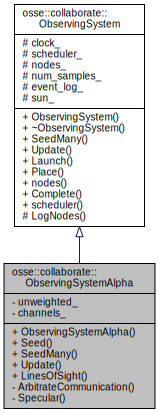
\includegraphics[width=231pt]{classosse_1_1collaborate_1_1_observing_system_alpha__inherit__graph}
\end{center}
\end{figure}
\subsubsection*{Public Member Functions}
\begin{DoxyCompactItemize}
\item 
\hyperlink{classosse_1_1collaborate_1_1_observing_system_alpha_ab282044b92aabebc6d9d31e0c9ab84b6}{Observing\+System\+Alpha} (\hyperlink{classosse_1_1collaborate_1_1_sun}{Sun} $\ast$\+\_\+sun, \hyperlink{classosse_1_1collaborate_1_1_simulation_clock}{Simulation\+Clock} $\ast$\+\_\+clock, \hyperlink{classosse_1_1collaborate_1_1_scheduler}{Scheduler} $\ast$\+\_\+collaborate, \hyperlink{classosse_1_1collaborate_1_1_event_logger}{Event\+Logger} $\ast$\+\_\+event\+\_\+log, \hyperlink{classosse_1_1collaborate_1_1_data_logger}{Data\+Logger} $\ast$\+\_\+network\+\_\+log)
\begin{DoxyCompactList}\small\item\em Constructor. \end{DoxyCompactList}\item 
\hyperlink{classosse_1_1collaborate_1_1_observing_system_alpha_a4f22ecd7429656408684eba1adf5d62e}{Observing\+System\+Alpha} (\hyperlink{classosse_1_1collaborate_1_1_sun}{Sun} $\ast$\+\_\+sun, \hyperlink{classosse_1_1collaborate_1_1_simulation_clock}{Simulation\+Clock} $\ast$\+\_\+clock, \hyperlink{classosse_1_1collaborate_1_1_scheduler}{Scheduler} $\ast$\+\_\+collaborate, \hyperlink{classosse_1_1collaborate_1_1_event_logger}{Event\+Logger} $\ast$\+\_\+event\+\_\+log, \hyperlink{classosse_1_1collaborate_1_1_data_logger}{Data\+Logger} $\ast$\+\_\+network\+\_\+log, const bool \&\+\_\+flag)
\begin{DoxyCompactList}\small\item\em Constructor. \end{DoxyCompactList}\item 
void \hyperlink{classosse_1_1collaborate_1_1_observing_system_alpha_a99b9d34ab9304624d36253d4431d34e7}{Seed} (const uint64\+\_\+t \&\+\_\+span\+\_\+s)
\begin{DoxyCompactList}\small\item\em Generates random list of samples to start with. \end{DoxyCompactList}\item 
void \hyperlink{classosse_1_1collaborate_1_1_observing_system_alpha_a6f6e7a1f24d7890c9da666e9e90ecb2b}{Seed\+Many} (const uint64\+\_\+t \&\+\_\+span\+\_\+s, const uint16\+\_\+t \&\+\_\+constellation)
\begin{DoxyCompactList}\small\item\em Generates random list of samples to start with for a constellation. \end{DoxyCompactList}\item 
void \hyperlink{classosse_1_1collaborate_1_1_observing_system_alpha_ad720f4060e443b244540333b6e5d27a8}{Seed\+Many\+More} (const uint64\+\_\+t \&\+\_\+span\+\_\+s, const uint16\+\_\+t \&\+\_\+constellation)
\begin{DoxyCompactList}\small\item\em Generates random list of samples to start with for a constellation. \end{DoxyCompactList}\item 
\mbox{\Hypertarget{classosse_1_1collaborate_1_1_observing_system_alpha_aa08dadc203f46736cc75d4a1a5ef60f8}\label{classosse_1_1collaborate_1_1_observing_system_alpha_aa08dadc203f46736cc75d4a1a5ef60f8}} 
void \hyperlink{classosse_1_1collaborate_1_1_observing_system_alpha_aa08dadc203f46736cc75d4a1a5ef60f8}{Update} ()
\begin{DoxyCompactList}\small\item\em Update everything. \end{DoxyCompactList}\item 
\mbox{\Hypertarget{classosse_1_1collaborate_1_1_observing_system_alpha_a8a7798f3de1f2b96524d1457d9f3143f}\label{classosse_1_1collaborate_1_1_observing_system_alpha_a8a7798f3de1f2b96524d1457d9f3143f}} 
void \hyperlink{classosse_1_1collaborate_1_1_observing_system_alpha_a8a7798f3de1f2b96524d1457d9f3143f}{Lines\+Of\+Sight} ()
\begin{DoxyCompactList}\small\item\em Calculate all lines of sight between satellites and write log. \end{DoxyCompactList}\end{DoxyCompactItemize}
\subsubsection*{Private Member Functions}
\begin{DoxyCompactItemize}
\item 
\mbox{\Hypertarget{classosse_1_1collaborate_1_1_observing_system_alpha_a19bf647d15aeb16d71082e1aef2ba140}\label{classosse_1_1collaborate_1_1_observing_system_alpha_a19bf647d15aeb16d71082e1aef2ba140}} 
void \hyperlink{classosse_1_1collaborate_1_1_observing_system_alpha_a19bf647d15aeb16d71082e1aef2ba140}{Arbitrate\+Communication} ()
\begin{DoxyCompactList}\small\item\em Creates new channels for nodes needing to communicate. \end{DoxyCompactList}\item 
\mbox{\Hypertarget{classosse_1_1collaborate_1_1_observing_system_alpha_a28f5ffebc95dc94c95de69732ce8ee29}\label{classosse_1_1collaborate_1_1_observing_system_alpha_a28f5ffebc95dc94c95de69732ce8ee29}} 
void \hyperlink{classosse_1_1collaborate_1_1_observing_system_alpha_a28f5ffebc95dc94c95de69732ce8ee29}{Specular} ()
\begin{DoxyCompactList}\small\item\em Finds all specular points. \end{DoxyCompactList}\end{DoxyCompactItemize}
\subsubsection*{Private Attributes}
\begin{DoxyCompactItemize}
\item 
\mbox{\Hypertarget{classosse_1_1collaborate_1_1_observing_system_alpha_afb9f4173b5226b349365b7d529fa93e2}\label{classosse_1_1collaborate_1_1_observing_system_alpha_afb9f4173b5226b349365b7d529fa93e2}} 
\hyperlink{classosse_1_1collaborate_1_1_graph_unweighted}{Graph\+Unweighted} \hyperlink{classosse_1_1collaborate_1_1_observing_system_alpha_afb9f4173b5226b349365b7d529fa93e2}{unweighted\+\_\+}
\begin{DoxyCompactList}\small\item\em Active channels. \end{DoxyCompactList}\item 
\mbox{\Hypertarget{classosse_1_1collaborate_1_1_observing_system_alpha_a69f8f791a0d6289f2d043a4a2ec6912c}\label{classosse_1_1collaborate_1_1_observing_system_alpha_a69f8f791a0d6289f2d043a4a2ec6912c}} 
std\+::vector$<$ \hyperlink{classosse_1_1collaborate_1_1_channel}{Channel} $>$ \hyperlink{classosse_1_1collaborate_1_1_observing_system_alpha_a69f8f791a0d6289f2d043a4a2ec6912c}{channels\+\_\+}
\begin{DoxyCompactList}\small\item\em An adjacency attitude\+\_\+matrix. \end{DoxyCompactList}\item 
\mbox{\Hypertarget{classosse_1_1collaborate_1_1_observing_system_alpha_a5aaa729d1e8c2778865626843035e510}\label{classosse_1_1collaborate_1_1_observing_system_alpha_a5aaa729d1e8c2778865626843035e510}} 
bool \hyperlink{classosse_1_1collaborate_1_1_observing_system_alpha_a5aaa729d1e8c2778865626843035e510}{flag\+\_\+}
\begin{DoxyCompactList}\small\item\em Flag. \end{DoxyCompactList}\end{DoxyCompactItemize}
\subsubsection*{Additional Inherited Members}


\subsubsection{Detailed Description}
Concrete satellite observing system. 

 
\begin{DoxyImageNoCaption}
  \mbox{\includegraphics[width=\textwidth]{map}}
\end{DoxyImageNoCaption}
 

\subsubsection{Constructor \& Destructor Documentation}
\mbox{\Hypertarget{classosse_1_1collaborate_1_1_observing_system_alpha_ab282044b92aabebc6d9d31e0c9ab84b6}\label{classosse_1_1collaborate_1_1_observing_system_alpha_ab282044b92aabebc6d9d31e0c9ab84b6}} 
\index{osse\+::collaborate\+::\+Observing\+System\+Alpha@{osse\+::collaborate\+::\+Observing\+System\+Alpha}!Observing\+System\+Alpha@{Observing\+System\+Alpha}}
\index{Observing\+System\+Alpha@{Observing\+System\+Alpha}!osse\+::collaborate\+::\+Observing\+System\+Alpha@{osse\+::collaborate\+::\+Observing\+System\+Alpha}}
\paragraph{\texorpdfstring{Observing\+System\+Alpha()}{ObservingSystemAlpha()}\hspace{0.1cm}{\footnotesize\ttfamily [1/2]}}
{\footnotesize\ttfamily osse\+::collaborate\+::\+Observing\+System\+Alpha\+::\+Observing\+System\+Alpha (\begin{DoxyParamCaption}\item[{\hyperlink{classosse_1_1collaborate_1_1_sun}{Sun} $\ast$}]{\+\_\+sun,  }\item[{\hyperlink{classosse_1_1collaborate_1_1_simulation_clock}{Simulation\+Clock} $\ast$}]{\+\_\+clock,  }\item[{\hyperlink{classosse_1_1collaborate_1_1_scheduler}{Scheduler} $\ast$}]{\+\_\+collaborate,  }\item[{\hyperlink{classosse_1_1collaborate_1_1_event_logger}{Event\+Logger} $\ast$}]{\+\_\+event\+\_\+log,  }\item[{\hyperlink{classosse_1_1collaborate_1_1_data_logger}{Data\+Logger} $\ast$}]{\+\_\+network\+\_\+log }\end{DoxyParamCaption})}



Constructor. 


\begin{DoxyParams}[1]{Parameters}
\mbox{\tt in}  & {\em \+\_\+sun} & Star at the center of the solar system \\
\hline
\mbox{\tt in}  & {\em \+\_\+clock} & Simulation clock \\
\hline
\mbox{\tt in}  & {\em \+\_\+collaborate} & Autonomous network collaborate \\
\hline
\mbox{\tt in}  & {\em \+\_\+event\+\_\+log} & Event logger \\
\hline
\mbox{\tt in}  & {\em \+\_\+network\+\_\+log} & Network logger \\
\hline
\end{DoxyParams}
\mbox{\Hypertarget{classosse_1_1collaborate_1_1_observing_system_alpha_a4f22ecd7429656408684eba1adf5d62e}\label{classosse_1_1collaborate_1_1_observing_system_alpha_a4f22ecd7429656408684eba1adf5d62e}} 
\index{osse\+::collaborate\+::\+Observing\+System\+Alpha@{osse\+::collaborate\+::\+Observing\+System\+Alpha}!Observing\+System\+Alpha@{Observing\+System\+Alpha}}
\index{Observing\+System\+Alpha@{Observing\+System\+Alpha}!osse\+::collaborate\+::\+Observing\+System\+Alpha@{osse\+::collaborate\+::\+Observing\+System\+Alpha}}
\paragraph{\texorpdfstring{Observing\+System\+Alpha()}{ObservingSystemAlpha()}\hspace{0.1cm}{\footnotesize\ttfamily [2/2]}}
{\footnotesize\ttfamily osse\+::collaborate\+::\+Observing\+System\+Alpha\+::\+Observing\+System\+Alpha (\begin{DoxyParamCaption}\item[{\hyperlink{classosse_1_1collaborate_1_1_sun}{Sun} $\ast$}]{\+\_\+sun,  }\item[{\hyperlink{classosse_1_1collaborate_1_1_simulation_clock}{Simulation\+Clock} $\ast$}]{\+\_\+clock,  }\item[{\hyperlink{classosse_1_1collaborate_1_1_scheduler}{Scheduler} $\ast$}]{\+\_\+collaborate,  }\item[{\hyperlink{classosse_1_1collaborate_1_1_event_logger}{Event\+Logger} $\ast$}]{\+\_\+event\+\_\+log,  }\item[{\hyperlink{classosse_1_1collaborate_1_1_data_logger}{Data\+Logger} $\ast$}]{\+\_\+network\+\_\+log,  }\item[{const bool \&}]{\+\_\+flag }\end{DoxyParamCaption})}



Constructor. 


\begin{DoxyParams}[1]{Parameters}
\mbox{\tt in}  & {\em \+\_\+sun} & Star at the center of the solar system \\
\hline
\mbox{\tt in}  & {\em \+\_\+clock} & Simulation clock \\
\hline
\mbox{\tt in}  & {\em \+\_\+collaborate} & Autonomous network collaborate \\
\hline
\mbox{\tt in}  & {\em \+\_\+event\+\_\+log} & Event logger \\
\hline
\mbox{\tt in}  & {\em \+\_\+network\+\_\+log} & Network logger \\
\hline
\mbox{\tt in}  & {\em \+\_\+flag} & Flag \\
\hline
\end{DoxyParams}


\subsubsection{Member Function Documentation}
\mbox{\Hypertarget{classosse_1_1collaborate_1_1_observing_system_alpha_a99b9d34ab9304624d36253d4431d34e7}\label{classosse_1_1collaborate_1_1_observing_system_alpha_a99b9d34ab9304624d36253d4431d34e7}} 
\index{osse\+::collaborate\+::\+Observing\+System\+Alpha@{osse\+::collaborate\+::\+Observing\+System\+Alpha}!Seed@{Seed}}
\index{Seed@{Seed}!osse\+::collaborate\+::\+Observing\+System\+Alpha@{osse\+::collaborate\+::\+Observing\+System\+Alpha}}
\paragraph{\texorpdfstring{Seed()}{Seed()}}
{\footnotesize\ttfamily void osse\+::collaborate\+::\+Observing\+System\+Alpha\+::\+Seed (\begin{DoxyParamCaption}\item[{const uint64\+\_\+t \&}]{\+\_\+span\+\_\+s }\end{DoxyParamCaption})}



Generates random list of samples to start with. 


\begin{DoxyParams}[1]{Parameters}
\mbox{\tt in}  & {\em \+\_\+span\+\_\+s} & Total time span of the simulation \\
\hline
\end{DoxyParams}
\mbox{\Hypertarget{classosse_1_1collaborate_1_1_observing_system_alpha_a6f6e7a1f24d7890c9da666e9e90ecb2b}\label{classosse_1_1collaborate_1_1_observing_system_alpha_a6f6e7a1f24d7890c9da666e9e90ecb2b}} 
\index{osse\+::collaborate\+::\+Observing\+System\+Alpha@{osse\+::collaborate\+::\+Observing\+System\+Alpha}!Seed\+Many@{Seed\+Many}}
\index{Seed\+Many@{Seed\+Many}!osse\+::collaborate\+::\+Observing\+System\+Alpha@{osse\+::collaborate\+::\+Observing\+System\+Alpha}}
\paragraph{\texorpdfstring{Seed\+Many()}{SeedMany()}}
{\footnotesize\ttfamily void osse\+::collaborate\+::\+Observing\+System\+Alpha\+::\+Seed\+Many (\begin{DoxyParamCaption}\item[{const uint64\+\_\+t \&}]{\+\_\+span\+\_\+s,  }\item[{const uint16\+\_\+t \&}]{\+\_\+constellation }\end{DoxyParamCaption})\hspace{0.3cm}{\ttfamily [virtual]}}



Generates random list of samples to start with for a constellation. 


\begin{DoxyParams}[1]{Parameters}
\mbox{\tt in}  & {\em \+\_\+span\+\_\+s} & Total time span of the simulation \\
\hline
\mbox{\tt in}  & {\em \+\_\+constellation} & Constellation \\
\hline
\end{DoxyParams}


Implements \hyperlink{classosse_1_1collaborate_1_1_observing_system_ae324ec9fd51b8e65afd80292748b406c}{osse\+::collaborate\+::\+Observing\+System}.

\mbox{\Hypertarget{classosse_1_1collaborate_1_1_observing_system_alpha_ad720f4060e443b244540333b6e5d27a8}\label{classosse_1_1collaborate_1_1_observing_system_alpha_ad720f4060e443b244540333b6e5d27a8}} 
\index{osse\+::collaborate\+::\+Observing\+System\+Alpha@{osse\+::collaborate\+::\+Observing\+System\+Alpha}!Seed\+Many\+More@{Seed\+Many\+More}}
\index{Seed\+Many\+More@{Seed\+Many\+More}!osse\+::collaborate\+::\+Observing\+System\+Alpha@{osse\+::collaborate\+::\+Observing\+System\+Alpha}}
\paragraph{\texorpdfstring{Seed\+Many\+More()}{SeedManyMore()}}
{\footnotesize\ttfamily void osse\+::collaborate\+::\+Observing\+System\+Alpha\+::\+Seed\+Many\+More (\begin{DoxyParamCaption}\item[{const uint64\+\_\+t \&}]{\+\_\+span\+\_\+s,  }\item[{const uint16\+\_\+t \&}]{\+\_\+constellation }\end{DoxyParamCaption})}



Generates random list of samples to start with for a constellation. 


\begin{DoxyParams}[1]{Parameters}
\mbox{\tt in}  & {\em \+\_\+span\+\_\+s} & Total time span of the simulation \\
\hline
\mbox{\tt in}  & {\em \+\_\+constellation} & Constellation \\
\hline
\end{DoxyParams}


The documentation for this class was generated from the following files\+:\begin{DoxyCompactItemize}
\item 
libs/collaborate/include/collaborate/observing\+\_\+system\+\_\+alpha.\+h\item 
libs/collaborate/src/observing\+\_\+system\+\_\+alpha.\+cpp\end{DoxyCompactItemize}

\hypertarget{classosse_1_1collaborate_1_1_observing_system}{}\subsection{osse\+:\+:collaborate\+:\+:Observing\+System Class Reference}
\label{classosse_1_1collaborate_1_1_observing_system}\index{osse\+::collaborate\+::\+Observing\+System@{osse\+::collaborate\+::\+Observing\+System}}


Abstract satellite network.  




{\ttfamily \#include $<$observing\+\_\+system.\+h$>$}



Inheritance diagram for osse\+:\+:collaborate\+:\+:Observing\+System\+:
\nopagebreak
\begin{figure}[H]
\begin{center}
\leavevmode
\includegraphics[width=231pt]{classosse_1_1collaborate_1_1_observing_system__inherit__graph}
\end{center}
\end{figure}
\subsubsection*{Public Member Functions}
\begin{DoxyCompactItemize}
\item 
\hyperlink{classosse_1_1collaborate_1_1_observing_system_a9cde3752308908b32f882ea8c529e7e2}{Observing\+System} (\hyperlink{classosse_1_1collaborate_1_1_sun}{Sun} $\ast$\+\_\+sun, \hyperlink{classosse_1_1collaborate_1_1_simulation_clock}{Simulation\+Clock} $\ast$\+\_\+clock, \hyperlink{classosse_1_1collaborate_1_1_scheduler}{Scheduler} $\ast$\+\_\+scheduler, \hyperlink{classosse_1_1collaborate_1_1_event_logger}{Event\+Logger} $\ast$\+\_\+event\+\_\+log)
\begin{DoxyCompactList}\small\item\em Constructor. \end{DoxyCompactList}\item 
\mbox{\Hypertarget{classosse_1_1collaborate_1_1_observing_system_a552670acae91c52b06296a0118e7871b}\label{classosse_1_1collaborate_1_1_observing_system_a552670acae91c52b06296a0118e7871b}} 
\hyperlink{classosse_1_1collaborate_1_1_observing_system_a552670acae91c52b06296a0118e7871b}{$\sim$\+Observing\+System} ()
\begin{DoxyCompactList}\small\item\em Destructor. \end{DoxyCompactList}\item 
virtual void \hyperlink{classosse_1_1collaborate_1_1_observing_system_ae324ec9fd51b8e65afd80292748b406c}{Seed\+Many} (const uint64\+\_\+t \&\+\_\+span\+\_\+s, const uint16\+\_\+t \&\+\_\+constellation)=0
\begin{DoxyCompactList}\small\item\em Generates random list of samples to start with. \end{DoxyCompactList}\item 
\mbox{\Hypertarget{classosse_1_1collaborate_1_1_observing_system_a8ebba43b54a5c7bb28e7721e7b1f8d9b}\label{classosse_1_1collaborate_1_1_observing_system_a8ebba43b54a5c7bb28e7721e7b1f8d9b}} 
virtual void \hyperlink{classosse_1_1collaborate_1_1_observing_system_a8ebba43b54a5c7bb28e7721e7b1f8d9b}{Update} ()=0
\begin{DoxyCompactList}\small\item\em Update the nodes and protocol. \end{DoxyCompactList}\item 
void \hyperlink{classosse_1_1collaborate_1_1_observing_system_af0d0030fd4d55ca3ac12bd65074d5b7d}{Launch} (const std\+::vector$<$ \hyperlink{classosse_1_1collaborate_1_1_platform_orbit}{Platform\+Orbit} $>$ \&\+\_\+orbits, const uint16\+\_\+t \&\+\_\+constellation, const bool \&\+\_\+separate, const \hyperlink{classosse_1_1collaborate_1_1_subsystem_comm}{Subsystem\+Comm} \&\+\_\+comm\+\_\+if, const \hyperlink{classosse_1_1collaborate_1_1_subsystem_sensing}{Subsystem\+Sensing} \&\+\_\+sensing\+\_\+if, const \hyperlink{classosse_1_1collaborate_1_1_subsystem_power}{Subsystem\+Power} \&\+\_\+subsystem\+\_\+power, \hyperlink{classosse_1_1collaborate_1_1_data_processor}{Data\+Processor} $\ast$\+\_\+data\+\_\+processor, \hyperlink{classosse_1_1collaborate_1_1_data_logger}{Data\+Logger} $\ast$\+\_\+data\+\_\+log)
\begin{DoxyCompactList}\small\item\em Make new nodes from a list of platforms. \end{DoxyCompactList}\item 
void \hyperlink{classosse_1_1collaborate_1_1_observing_system_a083b14c76f2e4af95d0228435b0644a4}{Place} (const std\+::vector$<$ \hyperlink{classosse_1_1collaborate_1_1_platform_earth}{Platform\+Earth} $>$ \&\+\_\+earths, const uint16\+\_\+t \&\+\_\+constellation, const bool \&\+\_\+separate, const \hyperlink{classosse_1_1collaborate_1_1_subsystem_comm}{Subsystem\+Comm} \&\+\_\+comm\+\_\+if, const \hyperlink{classosse_1_1collaborate_1_1_subsystem_sensing}{Subsystem\+Sensing} \&\+\_\+sensing\+\_\+if, const \hyperlink{classosse_1_1collaborate_1_1_subsystem_power}{Subsystem\+Power} \&\+\_\+subsystem\+\_\+power, \hyperlink{classosse_1_1collaborate_1_1_data_processor}{Data\+Processor} $\ast$\+\_\+data\+\_\+processor, \hyperlink{classosse_1_1collaborate_1_1_data_logger}{Data\+Logger} $\ast$\+\_\+data\+\_\+log)
\begin{DoxyCompactList}\small\item\em Make new nodes from a list of platforms. \end{DoxyCompactList}\item 
std\+::vector$<$ \hyperlink{classosse_1_1collaborate_1_1_node}{Node} $\ast$ $>$ \hyperlink{classosse_1_1collaborate_1_1_observing_system_ab870ae4c9e01fdf97682908857d882ed}{nodes} () const
\begin{DoxyCompactList}\small\item\em Get the earth\+\_\+data of nodes. \end{DoxyCompactList}\item 
\mbox{\Hypertarget{classosse_1_1collaborate_1_1_observing_system_a11c8616261fcf49fe02cddcfb662712c}\label{classosse_1_1collaborate_1_1_observing_system_a11c8616261fcf49fe02cddcfb662712c}} 
void \hyperlink{classosse_1_1collaborate_1_1_observing_system_a11c8616261fcf49fe02cddcfb662712c}{Complete} () const
\begin{DoxyCompactList}\small\item\em Logs the nodes at the end. \end{DoxyCompactList}\item 
\hyperlink{classosse_1_1collaborate_1_1_scheduler}{Scheduler} $\ast$ \hyperlink{classosse_1_1collaborate_1_1_observing_system_aaf4978922f6cdc6f361905a0523ce8a5}{scheduler} ()
\begin{DoxyCompactList}\small\item\em Get the scheduler. \end{DoxyCompactList}\end{DoxyCompactItemize}
\subsubsection*{Protected Member Functions}
\begin{DoxyCompactItemize}
\item 
\mbox{\Hypertarget{classosse_1_1collaborate_1_1_observing_system_afd35e353e3bfa35992269ec9310995d8}\label{classosse_1_1collaborate_1_1_observing_system_afd35e353e3bfa35992269ec9310995d8}} 
void \hyperlink{classosse_1_1collaborate_1_1_observing_system_afd35e353e3bfa35992269ec9310995d8}{Log\+Nodes} () const
\begin{DoxyCompactList}\small\item\em Logs the nodes. \end{DoxyCompactList}\end{DoxyCompactItemize}
\subsubsection*{Protected Attributes}
\begin{DoxyCompactItemize}
\item 
\mbox{\Hypertarget{classosse_1_1collaborate_1_1_observing_system_a4aba07ee9f871dbc59e1a9cee69b3df1}\label{classosse_1_1collaborate_1_1_observing_system_a4aba07ee9f871dbc59e1a9cee69b3df1}} 
const \hyperlink{classosse_1_1collaborate_1_1_simulation_clock}{Simulation\+Clock} $\ast$ \hyperlink{classosse_1_1collaborate_1_1_observing_system_a4aba07ee9f871dbc59e1a9cee69b3df1}{clock\+\_\+}
\begin{DoxyCompactList}\small\item\em \hyperlink{classosse_1_1collaborate_1_1_simulation_clock}{Simulation\+Clock}. \end{DoxyCompactList}\item 
\mbox{\Hypertarget{classosse_1_1collaborate_1_1_observing_system_ab806285bde05f87bdb89c7636eb20bd8}\label{classosse_1_1collaborate_1_1_observing_system_ab806285bde05f87bdb89c7636eb20bd8}} 
\hyperlink{classosse_1_1collaborate_1_1_scheduler}{Scheduler} $\ast$ \hyperlink{classosse_1_1collaborate_1_1_observing_system_ab806285bde05f87bdb89c7636eb20bd8}{scheduler\+\_\+}
\begin{DoxyCompactList}\small\item\em Autonomous network scheduler. \end{DoxyCompactList}\item 
\mbox{\Hypertarget{classosse_1_1collaborate_1_1_observing_system_a61f8db4cc88e53cc644e43424aa6e9e4}\label{classosse_1_1collaborate_1_1_observing_system_a61f8db4cc88e53cc644e43424aa6e9e4}} 
std\+::vector$<$ \hyperlink{classosse_1_1collaborate_1_1_node}{Node} $\ast$ $>$ \hyperlink{classosse_1_1collaborate_1_1_observing_system_a61f8db4cc88e53cc644e43424aa6e9e4}{nodes\+\_\+}
\begin{DoxyCompactList}\small\item\em Ordered list of nodes. \end{DoxyCompactList}\item 
\mbox{\Hypertarget{classosse_1_1collaborate_1_1_observing_system_a44cdbb8ac2fc877e3e0efee778e3fc22}\label{classosse_1_1collaborate_1_1_observing_system_a44cdbb8ac2fc877e3e0efee778e3fc22}} 
uint64\+\_\+t \hyperlink{classosse_1_1collaborate_1_1_observing_system_a44cdbb8ac2fc877e3e0efee778e3fc22}{num\+\_\+samples\+\_\+}
\begin{DoxyCompactList}\small\item\em Number of samples seeded. \end{DoxyCompactList}\item 
\mbox{\Hypertarget{classosse_1_1collaborate_1_1_observing_system_ac3f97c3eb20163b20076f35ce78175ee}\label{classosse_1_1collaborate_1_1_observing_system_ac3f97c3eb20163b20076f35ce78175ee}} 
\hyperlink{classosse_1_1collaborate_1_1_event_logger}{Event\+Logger} $\ast$ \hyperlink{classosse_1_1collaborate_1_1_observing_system_ac3f97c3eb20163b20076f35ce78175ee}{event\+\_\+log\+\_\+}
\begin{DoxyCompactList}\small\item\em Event logger. \end{DoxyCompactList}\item 
\mbox{\Hypertarget{classosse_1_1collaborate_1_1_observing_system_aa6de5a15a22658a10220b163ee1d21d0}\label{classosse_1_1collaborate_1_1_observing_system_aa6de5a15a22658a10220b163ee1d21d0}} 
\hyperlink{classosse_1_1collaborate_1_1_sun}{Sun} $\ast$ \hyperlink{classosse_1_1collaborate_1_1_observing_system_aa6de5a15a22658a10220b163ee1d21d0}{sun\+\_\+}
\begin{DoxyCompactList}\small\item\em \hyperlink{classosse_1_1collaborate_1_1_sun}{Sun}. \end{DoxyCompactList}\end{DoxyCompactItemize}


\subsubsection{Detailed Description}
Abstract satellite network. 

 
\begin{DoxyImageNoCaption}
  \mbox{\includegraphics[width=\textwidth]{map}}
\end{DoxyImageNoCaption}
 

\subsubsection{Constructor \& Destructor Documentation}
\mbox{\Hypertarget{classosse_1_1collaborate_1_1_observing_system_a9cde3752308908b32f882ea8c529e7e2}\label{classosse_1_1collaborate_1_1_observing_system_a9cde3752308908b32f882ea8c529e7e2}} 
\index{osse\+::collaborate\+::\+Observing\+System@{osse\+::collaborate\+::\+Observing\+System}!Observing\+System@{Observing\+System}}
\index{Observing\+System@{Observing\+System}!osse\+::collaborate\+::\+Observing\+System@{osse\+::collaborate\+::\+Observing\+System}}
\paragraph{\texorpdfstring{Observing\+System()}{ObservingSystem()}}
{\footnotesize\ttfamily osse\+::collaborate\+::\+Observing\+System\+::\+Observing\+System (\begin{DoxyParamCaption}\item[{\hyperlink{classosse_1_1collaborate_1_1_sun}{Sun} $\ast$}]{\+\_\+sun,  }\item[{\hyperlink{classosse_1_1collaborate_1_1_simulation_clock}{Simulation\+Clock} $\ast$}]{\+\_\+clock,  }\item[{\hyperlink{classosse_1_1collaborate_1_1_scheduler}{Scheduler} $\ast$}]{\+\_\+scheduler,  }\item[{\hyperlink{classosse_1_1collaborate_1_1_event_logger}{Event\+Logger} $\ast$}]{\+\_\+event\+\_\+log }\end{DoxyParamCaption})}



Constructor. 


\begin{DoxyParams}[1]{Parameters}
\mbox{\tt in}  & {\em \+\_\+sun} & Star at the center of the solar system \\
\hline
\mbox{\tt in}  & {\em \+\_\+clock} & Simulation clock \\
\hline
\mbox{\tt in}  & {\em \+\_\+scheduler} & \hyperlink{classosse_1_1collaborate_1_1_scheduler}{Scheduler} \\
\hline
\mbox{\tt in}  & {\em \+\_\+event\+\_\+log} & Event log \\
\hline
\end{DoxyParams}


\subsubsection{Member Function Documentation}
\mbox{\Hypertarget{classosse_1_1collaborate_1_1_observing_system_af0d0030fd4d55ca3ac12bd65074d5b7d}\label{classosse_1_1collaborate_1_1_observing_system_af0d0030fd4d55ca3ac12bd65074d5b7d}} 
\index{osse\+::collaborate\+::\+Observing\+System@{osse\+::collaborate\+::\+Observing\+System}!Launch@{Launch}}
\index{Launch@{Launch}!osse\+::collaborate\+::\+Observing\+System@{osse\+::collaborate\+::\+Observing\+System}}
\paragraph{\texorpdfstring{Launch()}{Launch()}}
{\footnotesize\ttfamily void osse\+::collaborate\+::\+Observing\+System\+::\+Launch (\begin{DoxyParamCaption}\item[{const std\+::vector$<$ \hyperlink{classosse_1_1collaborate_1_1_platform_orbit}{Platform\+Orbit} $>$ \&}]{\+\_\+orbits,  }\item[{const uint16\+\_\+t \&}]{\+\_\+constellation,  }\item[{const bool \&}]{\+\_\+separate,  }\item[{const \hyperlink{classosse_1_1collaborate_1_1_subsystem_comm}{Subsystem\+Comm} \&}]{\+\_\+comm\+\_\+if,  }\item[{const \hyperlink{classosse_1_1collaborate_1_1_subsystem_sensing}{Subsystem\+Sensing} \&}]{\+\_\+sensing\+\_\+if,  }\item[{const \hyperlink{classosse_1_1collaborate_1_1_subsystem_power}{Subsystem\+Power} \&}]{\+\_\+subsystem\+\_\+power,  }\item[{\hyperlink{classosse_1_1collaborate_1_1_data_processor}{Data\+Processor} $\ast$}]{\+\_\+data\+\_\+processor,  }\item[{\hyperlink{classosse_1_1collaborate_1_1_data_logger}{Data\+Logger} $\ast$}]{\+\_\+data\+\_\+log }\end{DoxyParamCaption})}



Make new nodes from a list of platforms. 


\begin{DoxyParams}[1]{Parameters}
\mbox{\tt in}  & {\em \+\_\+orbits} & List of orbits \\
\hline
\mbox{\tt in}  & {\em \+\_\+constellation} & Starting constellation identifier \\
\hline
\mbox{\tt in}  & {\em \+\_\+separate} & Whether the nodess are separate constellations \\
\hline
\mbox{\tt in}  & {\em \+\_\+comm\+\_\+if} & Communication interface \\
\hline
\mbox{\tt in}  & {\em \+\_\+sensing\+\_\+if} & Sensing interface \\
\hline
\mbox{\tt in}  & {\em \+\_\+subsystem\+\_\+power} & Power subsystem \\
\hline
\mbox{\tt in}  & {\em \+\_\+data\+\_\+processor} & Data processor \\
\hline
\mbox{\tt in}  & {\em \+\_\+data\+\_\+log} & Data logger \\
\hline
\end{DoxyParams}
\mbox{\Hypertarget{classosse_1_1collaborate_1_1_observing_system_ab870ae4c9e01fdf97682908857d882ed}\label{classosse_1_1collaborate_1_1_observing_system_ab870ae4c9e01fdf97682908857d882ed}} 
\index{osse\+::collaborate\+::\+Observing\+System@{osse\+::collaborate\+::\+Observing\+System}!nodes@{nodes}}
\index{nodes@{nodes}!osse\+::collaborate\+::\+Observing\+System@{osse\+::collaborate\+::\+Observing\+System}}
\paragraph{\texorpdfstring{nodes()}{nodes()}}
{\footnotesize\ttfamily std\+::vector$<$\hyperlink{classosse_1_1collaborate_1_1_node}{Node}$\ast$$>$ osse\+::collaborate\+::\+Observing\+System\+::nodes (\begin{DoxyParamCaption}{ }\end{DoxyParamCaption}) const\hspace{0.3cm}{\ttfamily [inline]}}



Get the earth\+\_\+data of nodes. 

\begin{DoxyReturn}{Returns}
nodes\+\_\+ The earth\+\_\+data of nodes 
\end{DoxyReturn}
\mbox{\Hypertarget{classosse_1_1collaborate_1_1_observing_system_a083b14c76f2e4af95d0228435b0644a4}\label{classosse_1_1collaborate_1_1_observing_system_a083b14c76f2e4af95d0228435b0644a4}} 
\index{osse\+::collaborate\+::\+Observing\+System@{osse\+::collaborate\+::\+Observing\+System}!Place@{Place}}
\index{Place@{Place}!osse\+::collaborate\+::\+Observing\+System@{osse\+::collaborate\+::\+Observing\+System}}
\paragraph{\texorpdfstring{Place()}{Place()}}
{\footnotesize\ttfamily void osse\+::collaborate\+::\+Observing\+System\+::\+Place (\begin{DoxyParamCaption}\item[{const std\+::vector$<$ \hyperlink{classosse_1_1collaborate_1_1_platform_earth}{Platform\+Earth} $>$ \&}]{\+\_\+earths,  }\item[{const uint16\+\_\+t \&}]{\+\_\+constellation,  }\item[{const bool \&}]{\+\_\+separate,  }\item[{const \hyperlink{classosse_1_1collaborate_1_1_subsystem_comm}{Subsystem\+Comm} \&}]{\+\_\+comm\+\_\+if,  }\item[{const \hyperlink{classosse_1_1collaborate_1_1_subsystem_sensing}{Subsystem\+Sensing} \&}]{\+\_\+sensing\+\_\+if,  }\item[{const \hyperlink{classosse_1_1collaborate_1_1_subsystem_power}{Subsystem\+Power} \&}]{\+\_\+subsystem\+\_\+power,  }\item[{\hyperlink{classosse_1_1collaborate_1_1_data_processor}{Data\+Processor} $\ast$}]{\+\_\+data\+\_\+processor,  }\item[{\hyperlink{classosse_1_1collaborate_1_1_data_logger}{Data\+Logger} $\ast$}]{\+\_\+data\+\_\+log }\end{DoxyParamCaption})}



Make new nodes from a list of platforms. 


\begin{DoxyParams}[1]{Parameters}
\mbox{\tt in}  & {\em \+\_\+earths} & List of earth platforms \\
\hline
\mbox{\tt in}  & {\em \+\_\+constellation} & Starting constellation identifier \\
\hline
\mbox{\tt in}  & {\em \+\_\+separate} & Whether the nodess are separate constellations \\
\hline
\mbox{\tt in}  & {\em \+\_\+comm\+\_\+if} & The communication interface \\
\hline
\mbox{\tt in}  & {\em \+\_\+sensing\+\_\+if} & Sensing interface \\
\hline
\mbox{\tt in}  & {\em \+\_\+subsystem\+\_\+power} & Power subsystem \\
\hline
\mbox{\tt in}  & {\em \+\_\+data\+\_\+processor} & Data processor \\
\hline
\mbox{\tt in}  & {\em \+\_\+data\+\_\+log} & Data logger \\
\hline
\end{DoxyParams}
\mbox{\Hypertarget{classosse_1_1collaborate_1_1_observing_system_aaf4978922f6cdc6f361905a0523ce8a5}\label{classosse_1_1collaborate_1_1_observing_system_aaf4978922f6cdc6f361905a0523ce8a5}} 
\index{osse\+::collaborate\+::\+Observing\+System@{osse\+::collaborate\+::\+Observing\+System}!scheduler@{scheduler}}
\index{scheduler@{scheduler}!osse\+::collaborate\+::\+Observing\+System@{osse\+::collaborate\+::\+Observing\+System}}
\paragraph{\texorpdfstring{scheduler()}{scheduler()}}
{\footnotesize\ttfamily \hyperlink{classosse_1_1collaborate_1_1_scheduler}{Scheduler}$\ast$ osse\+::collaborate\+::\+Observing\+System\+::scheduler (\begin{DoxyParamCaption}{ }\end{DoxyParamCaption})\hspace{0.3cm}{\ttfamily [inline]}}



Get the scheduler. 

\begin{DoxyReturn}{Returns}
scheduler\+\_\+ \hyperlink{classosse_1_1collaborate_1_1_scheduler}{Scheduler} 
\end{DoxyReturn}
\mbox{\Hypertarget{classosse_1_1collaborate_1_1_observing_system_ae324ec9fd51b8e65afd80292748b406c}\label{classosse_1_1collaborate_1_1_observing_system_ae324ec9fd51b8e65afd80292748b406c}} 
\index{osse\+::collaborate\+::\+Observing\+System@{osse\+::collaborate\+::\+Observing\+System}!Seed\+Many@{Seed\+Many}}
\index{Seed\+Many@{Seed\+Many}!osse\+::collaborate\+::\+Observing\+System@{osse\+::collaborate\+::\+Observing\+System}}
\paragraph{\texorpdfstring{Seed\+Many()}{SeedMany()}}
{\footnotesize\ttfamily virtual void osse\+::collaborate\+::\+Observing\+System\+::\+Seed\+Many (\begin{DoxyParamCaption}\item[{const uint64\+\_\+t \&}]{\+\_\+span\+\_\+s,  }\item[{const uint16\+\_\+t \&}]{\+\_\+constellation }\end{DoxyParamCaption})\hspace{0.3cm}{\ttfamily [pure virtual]}}



Generates random list of samples to start with. 


\begin{DoxyParams}[1]{Parameters}
\mbox{\tt in}  & {\em \+\_\+span\+\_\+s} & Total time span of the simulation (seconds) \\
\hline
\mbox{\tt in}  & {\em \+\_\+constellation} & Constellation \\
\hline
\end{DoxyParams}


Implemented in \hyperlink{classosse_1_1collaborate_1_1_observing_system_alpha_a6f6e7a1f24d7890c9da666e9e90ecb2b}{osse\+::collaborate\+::\+Observing\+System\+Alpha}.



The documentation for this class was generated from the following files\+:\begin{DoxyCompactItemize}
\item 
libs/collaborate/include/collaborate/observing\+\_\+system.\+h\item 
libs/collaborate/src/observing\+\_\+system.\+cpp\end{DoxyCompactItemize}

\hypertarget{classosse_1_1collaborate_1_1_orbital_state}{}\subsection{osse\+:\+:collaborate\+:\+:Orbital\+State Class Reference}
\label{classosse_1_1collaborate_1_1_orbital_state}\index{osse\+::collaborate\+::\+Orbital\+State@{osse\+::collaborate\+::\+Orbital\+State}}


The position and orientation of a node.  




{\ttfamily \#include $<$orbital\+\_\+state.\+h$>$}

\subsubsection*{Public Member Functions}
\begin{DoxyCompactItemize}
\item 
\hyperlink{classosse_1_1collaborate_1_1_orbital_state_a9990f1fc348981b44c1a9c7781cb9b4f}{Orbital\+State} (double \+\_\+x\+\_\+m, double \+\_\+y\+\_\+m, double \+\_\+z\+\_\+m, double \+\_\+latitude\+\_\+rad, double \+\_\+longitude\+\_\+rad, double \+\_\+altitude\+\_\+m, double \+\_\+dx\+\_\+m\+\_\+per\+\_\+s, double \+\_\+dy\+\_\+m\+\_\+per\+\_\+s, double \+\_\+dz\+\_\+m\+\_\+per\+\_\+s, double \+\_\+roll\+\_\+rad, double \+\_\+pitch\+\_\+rad, double \+\_\+yaw\+\_\+rad)
\begin{DoxyCompactList}\small\item\em Constructor. \end{DoxyCompactList}\item 
\hyperlink{classosse_1_1collaborate_1_1_reference_frame}{Reference\+Frame} \hyperlink{classosse_1_1collaborate_1_1_orbital_state_a0ed1213527f9cbe7a6131feb4308046e}{Calculate\+Platform\+Orbit\+Reference\+Frame} () const
\begin{DoxyCompactList}\small\item\em Calculates the orbit reference\+\_\+frame. \end{DoxyCompactList}\item 
void \hyperlink{classosse_1_1collaborate_1_1_orbital_state_a29fea23801f7de2f5ad72888b15ca220}{Update} (double \+\_\+x\+\_\+m, double \+\_\+y\+\_\+m, double \+\_\+z\+\_\+m, double \+\_\+latitude\+\_\+rad, double \+\_\+longitude\+\_\+rad, double \+\_\+altitude\+\_\+m, double \+\_\+dx\+\_\+m\+\_\+per\+\_\+s, double \+\_\+dy\+\_\+m\+\_\+per\+\_\+s, double \+\_\+dz\+\_\+m\+\_\+per\+\_\+s)
\begin{DoxyCompactList}\small\item\em Update the orbital\+\_\+state. \end{DoxyCompactList}\item 
std\+::vector$<$ double $>$ \hyperlink{classosse_1_1collaborate_1_1_orbital_state_a010c89b843916c12e8d6ec4042787af6}{Obtain\+Log} () const
\begin{DoxyCompactList}\small\item\em Logs the \hyperlink{classosse_1_1collaborate_1_1_orbital_state}{Orbital\+State}. \end{DoxyCompactList}\item 
std\+::vector$<$ double $>$ \hyperlink{classosse_1_1collaborate_1_1_orbital_state_a5ef68d5b425411e26612f213ab406136}{Obtain\+Geodetic\+Log} () const
\begin{DoxyCompactList}\small\item\em Logs the \hyperlink{classosse_1_1collaborate_1_1_orbital_state}{Orbital\+State} \hyperlink{classosse_1_1collaborate_1_1_geodetic}{Geodetic} Coordinates. \end{DoxyCompactList}\item 
const \hyperlink{classosse_1_1collaborate_1_1_vector}{Vector} \& \hyperlink{classosse_1_1collaborate_1_1_orbital_state_a09eef3c4ce4d5a6aff3b6cee6e1dea0e}{position\+\_\+m\+\_\+rad} () const
\begin{DoxyCompactList}\small\item\em Get The position (meters and radians) \end{DoxyCompactList}\item 
const \hyperlink{classosse_1_1collaborate_1_1_vector}{Vector} \& \hyperlink{classosse_1_1collaborate_1_1_orbital_state_a2d52b42f0259367d91e2c247aea9522f}{velocity\+\_\+m\+\_\+per\+\_\+s} () const
\begin{DoxyCompactList}\small\item\em Get the velocity. \end{DoxyCompactList}\item 
const \hyperlink{classosse_1_1collaborate_1_1_geodetic}{Geodetic} \& \hyperlink{classosse_1_1collaborate_1_1_orbital_state_a7a6f749d24d80b5e5c08eb4a03857a31}{geodetic\+\_\+rad\+\_\+m} () const
\begin{DoxyCompactList}\small\item\em Get The geodetic position (radians and meters) \end{DoxyCompactList}\item 
const \hyperlink{classosse_1_1collaborate_1_1_reference_frame}{Reference\+Frame} \& \hyperlink{classosse_1_1collaborate_1_1_orbital_state_a9704e21bdf2ed6245b4b27e5a2911310}{orbit\+\_\+frame} () const
\begin{DoxyCompactList}\small\item\em Get the orbit\+\_\+frame. \end{DoxyCompactList}\item 
const \hyperlink{classosse_1_1collaborate_1_1_reference_frame}{Reference\+Frame} \& \hyperlink{classosse_1_1collaborate_1_1_orbital_state_a28b3414c74ad4ebe11d0e835dc9591ee}{body\+\_\+frame} () const
\begin{DoxyCompactList}\small\item\em Get the body\+\_\+frame. \end{DoxyCompactList}\end{DoxyCompactItemize}
\subsubsection*{Private Attributes}
\begin{DoxyCompactItemize}
\item 
\mbox{\Hypertarget{classosse_1_1collaborate_1_1_orbital_state_a5508edbd6215162be9483b371e95750c}\label{classosse_1_1collaborate_1_1_orbital_state_a5508edbd6215162be9483b371e95750c}} 
\hyperlink{classosse_1_1collaborate_1_1_vector}{Vector} \hyperlink{classosse_1_1collaborate_1_1_orbital_state_a5508edbd6215162be9483b371e95750c}{position\+\_\+m\+\_\+rad\+\_\+}
\begin{DoxyCompactList}\small\item\em Position (meters and radians) \end{DoxyCompactList}\item 
\mbox{\Hypertarget{classosse_1_1collaborate_1_1_orbital_state_a07d091b449bf6093c0f8c8568d6625bb}\label{classosse_1_1collaborate_1_1_orbital_state_a07d091b449bf6093c0f8c8568d6625bb}} 
\hyperlink{classosse_1_1collaborate_1_1_vector}{Vector} \hyperlink{classosse_1_1collaborate_1_1_orbital_state_a07d091b449bf6093c0f8c8568d6625bb}{velocity\+\_\+m\+\_\+per\+\_\+s\+\_\+}
\begin{DoxyCompactList}\small\item\em Velocity (meters per second) \end{DoxyCompactList}\item 
\mbox{\Hypertarget{classosse_1_1collaborate_1_1_orbital_state_a5129e6f49ed14ff382a4f62cabe4d80c}\label{classosse_1_1collaborate_1_1_orbital_state_a5129e6f49ed14ff382a4f62cabe4d80c}} 
\hyperlink{classosse_1_1collaborate_1_1_geodetic}{Geodetic} \hyperlink{classosse_1_1collaborate_1_1_orbital_state_a5129e6f49ed14ff382a4f62cabe4d80c}{geodetic\+\_\+rad\+\_\+m\+\_\+}
\begin{DoxyCompactList}\small\item\em \hyperlink{classosse_1_1collaborate_1_1_geodetic}{Geodetic} position (radians and meters) \end{DoxyCompactList}\item 
\mbox{\Hypertarget{classosse_1_1collaborate_1_1_orbital_state_aa8a60024082bf2c299abfea13aa24f5e}\label{classosse_1_1collaborate_1_1_orbital_state_aa8a60024082bf2c299abfea13aa24f5e}} 
\hyperlink{classosse_1_1collaborate_1_1_reference_frame}{Reference\+Frame} \hyperlink{classosse_1_1collaborate_1_1_orbital_state_aa8a60024082bf2c299abfea13aa24f5e}{orbit\+\_\+frame\+\_\+}
\begin{DoxyCompactList}\small\item\em \hyperlink{classosse_1_1collaborate_1_1_platform_orbit}{Platform\+Orbit} \hyperlink{classosse_1_1collaborate_1_1_reference_frame}{Reference\+Frame} (unit) \end{DoxyCompactList}\item 
\mbox{\Hypertarget{classosse_1_1collaborate_1_1_orbital_state_a3542ba071a7a50da3974a5766b089d58}\label{classosse_1_1collaborate_1_1_orbital_state_a3542ba071a7a50da3974a5766b089d58}} 
\hyperlink{classosse_1_1collaborate_1_1_reference_frame}{Reference\+Frame} \hyperlink{classosse_1_1collaborate_1_1_orbital_state_a3542ba071a7a50da3974a5766b089d58}{body\+\_\+frame\+\_\+}
\begin{DoxyCompactList}\small\item\em Body \hyperlink{classosse_1_1collaborate_1_1_reference_frame}{Reference\+Frame} (unit) \end{DoxyCompactList}\end{DoxyCompactItemize}


\subsubsection{Detailed Description}
The position and orientation of a node. 

\subsubsection{Constructor \& Destructor Documentation}
\mbox{\Hypertarget{classosse_1_1collaborate_1_1_orbital_state_a9990f1fc348981b44c1a9c7781cb9b4f}\label{classosse_1_1collaborate_1_1_orbital_state_a9990f1fc348981b44c1a9c7781cb9b4f}} 
\index{osse\+::collaborate\+::\+Orbital\+State@{osse\+::collaborate\+::\+Orbital\+State}!Orbital\+State@{Orbital\+State}}
\index{Orbital\+State@{Orbital\+State}!osse\+::collaborate\+::\+Orbital\+State@{osse\+::collaborate\+::\+Orbital\+State}}
\paragraph{\texorpdfstring{Orbital\+State()}{OrbitalState()}}
{\footnotesize\ttfamily osse\+::collaborate\+::\+Orbital\+State\+::\+Orbital\+State (\begin{DoxyParamCaption}\item[{double}]{\+\_\+x\+\_\+m,  }\item[{double}]{\+\_\+y\+\_\+m,  }\item[{double}]{\+\_\+z\+\_\+m,  }\item[{double}]{\+\_\+latitude\+\_\+rad,  }\item[{double}]{\+\_\+longitude\+\_\+rad,  }\item[{double}]{\+\_\+altitude\+\_\+m,  }\item[{double}]{\+\_\+dx\+\_\+m\+\_\+per\+\_\+s,  }\item[{double}]{\+\_\+dy\+\_\+m\+\_\+per\+\_\+s,  }\item[{double}]{\+\_\+dz\+\_\+m\+\_\+per\+\_\+s,  }\item[{double}]{\+\_\+roll\+\_\+rad,  }\item[{double}]{\+\_\+pitch\+\_\+rad,  }\item[{double}]{\+\_\+yaw\+\_\+rad }\end{DoxyParamCaption})}



Constructor. 


\begin{DoxyParams}[1]{Parameters}
\mbox{\tt in}  & {\em \+\_\+x\+\_\+m} & X-\/component of position (meters) \\
\hline
\mbox{\tt in}  & {\em \+\_\+y\+\_\+m} & Y-\/component of position (meters) \\
\hline
\mbox{\tt in}  & {\em \+\_\+z\+\_\+m} & Z-\/component of position (meters) \\
\hline
\mbox{\tt in}  & {\em \+\_\+latitude\+\_\+rad} & Latitude (radians) \\
\hline
\mbox{\tt in}  & {\em \+\_\+longitude\+\_\+rad} & Longitude (radians) \\
\hline
\mbox{\tt in}  & {\em \+\_\+altitude\+\_\+m} & Altitude (meters) \\
\hline
\mbox{\tt in}  & {\em \+\_\+dx\+\_\+m\+\_\+per\+\_\+s} & X-\/component of velocity (meters per second) \\
\hline
\mbox{\tt in}  & {\em \+\_\+dy\+\_\+m\+\_\+per\+\_\+s} & Y-\/component of velocity (meters per second) \\
\hline
\mbox{\tt in}  & {\em \+\_\+dz\+\_\+m\+\_\+per\+\_\+s} & Z-\/component of velocity (meters per second) \\
\hline
\mbox{\tt in}  & {\em \+\_\+roll\+\_\+rad} & Satellite\textquotesingle{}s roll angle (radians) \\
\hline
\mbox{\tt in}  & {\em \+\_\+pitch\+\_\+rad} & Satellite\textquotesingle{}s pitch angle (radians) \\
\hline
\mbox{\tt in}  & {\em \+\_\+yaw\+\_\+rad} & Satellite\textquotesingle{}s yaw angle (radians) \\
\hline
\end{DoxyParams}


\subsubsection{Member Function Documentation}
\mbox{\Hypertarget{classosse_1_1collaborate_1_1_orbital_state_a28b3414c74ad4ebe11d0e835dc9591ee}\label{classosse_1_1collaborate_1_1_orbital_state_a28b3414c74ad4ebe11d0e835dc9591ee}} 
\index{osse\+::collaborate\+::\+Orbital\+State@{osse\+::collaborate\+::\+Orbital\+State}!body\+\_\+frame@{body\+\_\+frame}}
\index{body\+\_\+frame@{body\+\_\+frame}!osse\+::collaborate\+::\+Orbital\+State@{osse\+::collaborate\+::\+Orbital\+State}}
\paragraph{\texorpdfstring{body\+\_\+frame()}{body\_frame()}}
{\footnotesize\ttfamily const \hyperlink{classosse_1_1collaborate_1_1_reference_frame}{Reference\+Frame}\& osse\+::collaborate\+::\+Orbital\+State\+::body\+\_\+frame (\begin{DoxyParamCaption}{ }\end{DoxyParamCaption}) const\hspace{0.3cm}{\ttfamily [inline]}}



Get the body\+\_\+frame. 

\begin{DoxyReturn}{Returns}
body\+\_\+frame\+\_\+ Body\+\_\+reference\+\_\+frame (unit) 
\end{DoxyReturn}
\mbox{\Hypertarget{classosse_1_1collaborate_1_1_orbital_state_a0ed1213527f9cbe7a6131feb4308046e}\label{classosse_1_1collaborate_1_1_orbital_state_a0ed1213527f9cbe7a6131feb4308046e}} 
\index{osse\+::collaborate\+::\+Orbital\+State@{osse\+::collaborate\+::\+Orbital\+State}!Calculate\+Platform\+Orbit\+Reference\+Frame@{Calculate\+Platform\+Orbit\+Reference\+Frame}}
\index{Calculate\+Platform\+Orbit\+Reference\+Frame@{Calculate\+Platform\+Orbit\+Reference\+Frame}!osse\+::collaborate\+::\+Orbital\+State@{osse\+::collaborate\+::\+Orbital\+State}}
\paragraph{\texorpdfstring{Calculate\+Platform\+Orbit\+Reference\+Frame()}{CalculatePlatformOrbitReferenceFrame()}}
{\footnotesize\ttfamily \hyperlink{classosse_1_1collaborate_1_1_reference_frame}{Reference\+Frame} osse\+::collaborate\+::\+Orbital\+State\+::\+Calculate\+Platform\+Orbit\+Reference\+Frame (\begin{DoxyParamCaption}{ }\end{DoxyParamCaption}) const}



Calculates the orbit reference\+\_\+frame. 

\begin{DoxyReturn}{Returns}
Orbit reference\+\_\+frame
\end{DoxyReturn}
\[ \hat{y} = \frac{-\vec{p}\times\vec{v}} {\left\lvert-\vec{p}\times\vec{v}\right\rvert} \] \[ \hat{z} = \frac{-\vec{p}}{\left\lvert-\vec{p}\right\rvert} \] \[ \hat{x} = \hat{y}\times\hat{z} \] \mbox{\Hypertarget{classosse_1_1collaborate_1_1_orbital_state_a7a6f749d24d80b5e5c08eb4a03857a31}\label{classosse_1_1collaborate_1_1_orbital_state_a7a6f749d24d80b5e5c08eb4a03857a31}} 
\index{osse\+::collaborate\+::\+Orbital\+State@{osse\+::collaborate\+::\+Orbital\+State}!geodetic\+\_\+rad\+\_\+m@{geodetic\+\_\+rad\+\_\+m}}
\index{geodetic\+\_\+rad\+\_\+m@{geodetic\+\_\+rad\+\_\+m}!osse\+::collaborate\+::\+Orbital\+State@{osse\+::collaborate\+::\+Orbital\+State}}
\paragraph{\texorpdfstring{geodetic\+\_\+rad\+\_\+m()}{geodetic\_rad\_m()}}
{\footnotesize\ttfamily const \hyperlink{classosse_1_1collaborate_1_1_geodetic}{Geodetic}\& osse\+::collaborate\+::\+Orbital\+State\+::geodetic\+\_\+rad\+\_\+m (\begin{DoxyParamCaption}{ }\end{DoxyParamCaption}) const\hspace{0.3cm}{\ttfamily [inline]}}



Get The geodetic position (radians and meters) 

\begin{DoxyReturn}{Returns}
geodetic\+\_\+rad\+\_\+m\+\_\+ \hyperlink{classosse_1_1collaborate_1_1_geodetic}{Geodetic} position (radians and meters) 
\end{DoxyReturn}
\mbox{\Hypertarget{classosse_1_1collaborate_1_1_orbital_state_a5ef68d5b425411e26612f213ab406136}\label{classosse_1_1collaborate_1_1_orbital_state_a5ef68d5b425411e26612f213ab406136}} 
\index{osse\+::collaborate\+::\+Orbital\+State@{osse\+::collaborate\+::\+Orbital\+State}!Obtain\+Geodetic\+Log@{Obtain\+Geodetic\+Log}}
\index{Obtain\+Geodetic\+Log@{Obtain\+Geodetic\+Log}!osse\+::collaborate\+::\+Orbital\+State@{osse\+::collaborate\+::\+Orbital\+State}}
\paragraph{\texorpdfstring{Obtain\+Geodetic\+Log()}{ObtainGeodeticLog()}}
{\footnotesize\ttfamily std\+::vector$<$ double $>$ osse\+::collaborate\+::\+Orbital\+State\+::\+Obtain\+Geodetic\+Log (\begin{DoxyParamCaption}{ }\end{DoxyParamCaption}) const}



Logs the \hyperlink{classosse_1_1collaborate_1_1_orbital_state}{Orbital\+State} \hyperlink{classosse_1_1collaborate_1_1_geodetic}{Geodetic} Coordinates. 

\begin{DoxyReturn}{Returns}
A vector of doubles 
\end{DoxyReturn}
\mbox{\Hypertarget{classosse_1_1collaborate_1_1_orbital_state_a010c89b843916c12e8d6ec4042787af6}\label{classosse_1_1collaborate_1_1_orbital_state_a010c89b843916c12e8d6ec4042787af6}} 
\index{osse\+::collaborate\+::\+Orbital\+State@{osse\+::collaborate\+::\+Orbital\+State}!Obtain\+Log@{Obtain\+Log}}
\index{Obtain\+Log@{Obtain\+Log}!osse\+::collaborate\+::\+Orbital\+State@{osse\+::collaborate\+::\+Orbital\+State}}
\paragraph{\texorpdfstring{Obtain\+Log()}{ObtainLog()}}
{\footnotesize\ttfamily std\+::vector$<$ double $>$ osse\+::collaborate\+::\+Orbital\+State\+::\+Obtain\+Log (\begin{DoxyParamCaption}{ }\end{DoxyParamCaption}) const}



Logs the \hyperlink{classosse_1_1collaborate_1_1_orbital_state}{Orbital\+State}. 

\begin{DoxyReturn}{Returns}
A vector of doubles 
\end{DoxyReturn}
\mbox{\Hypertarget{classosse_1_1collaborate_1_1_orbital_state_a9704e21bdf2ed6245b4b27e5a2911310}\label{classosse_1_1collaborate_1_1_orbital_state_a9704e21bdf2ed6245b4b27e5a2911310}} 
\index{osse\+::collaborate\+::\+Orbital\+State@{osse\+::collaborate\+::\+Orbital\+State}!orbit\+\_\+frame@{orbit\+\_\+frame}}
\index{orbit\+\_\+frame@{orbit\+\_\+frame}!osse\+::collaborate\+::\+Orbital\+State@{osse\+::collaborate\+::\+Orbital\+State}}
\paragraph{\texorpdfstring{orbit\+\_\+frame()}{orbit\_frame()}}
{\footnotesize\ttfamily const \hyperlink{classosse_1_1collaborate_1_1_reference_frame}{Reference\+Frame}\& osse\+::collaborate\+::\+Orbital\+State\+::orbit\+\_\+frame (\begin{DoxyParamCaption}{ }\end{DoxyParamCaption}) const\hspace{0.3cm}{\ttfamily [inline]}}



Get the orbit\+\_\+frame. 

\begin{DoxyReturn}{Returns}
orbit\+\_\+frame\+\_\+ Orbit\+\_\+reference\+\_\+frame (unit) 
\end{DoxyReturn}
\mbox{\Hypertarget{classosse_1_1collaborate_1_1_orbital_state_a09eef3c4ce4d5a6aff3b6cee6e1dea0e}\label{classosse_1_1collaborate_1_1_orbital_state_a09eef3c4ce4d5a6aff3b6cee6e1dea0e}} 
\index{osse\+::collaborate\+::\+Orbital\+State@{osse\+::collaborate\+::\+Orbital\+State}!position\+\_\+m\+\_\+rad@{position\+\_\+m\+\_\+rad}}
\index{position\+\_\+m\+\_\+rad@{position\+\_\+m\+\_\+rad}!osse\+::collaborate\+::\+Orbital\+State@{osse\+::collaborate\+::\+Orbital\+State}}
\paragraph{\texorpdfstring{position\+\_\+m\+\_\+rad()}{position\_m\_rad()}}
{\footnotesize\ttfamily const \hyperlink{classosse_1_1collaborate_1_1_vector}{Vector}\& osse\+::collaborate\+::\+Orbital\+State\+::position\+\_\+m\+\_\+rad (\begin{DoxyParamCaption}{ }\end{DoxyParamCaption}) const\hspace{0.3cm}{\ttfamily [inline]}}



Get The position (meters and radians) 

\begin{DoxyReturn}{Returns}
position\+\_\+m\+\_\+rad\+\_\+ Position (meters and radians) 
\end{DoxyReturn}
\mbox{\Hypertarget{classosse_1_1collaborate_1_1_orbital_state_a29fea23801f7de2f5ad72888b15ca220}\label{classosse_1_1collaborate_1_1_orbital_state_a29fea23801f7de2f5ad72888b15ca220}} 
\index{osse\+::collaborate\+::\+Orbital\+State@{osse\+::collaborate\+::\+Orbital\+State}!Update@{Update}}
\index{Update@{Update}!osse\+::collaborate\+::\+Orbital\+State@{osse\+::collaborate\+::\+Orbital\+State}}
\paragraph{\texorpdfstring{Update()}{Update()}}
{\footnotesize\ttfamily void osse\+::collaborate\+::\+Orbital\+State\+::\+Update (\begin{DoxyParamCaption}\item[{double}]{\+\_\+x\+\_\+m,  }\item[{double}]{\+\_\+y\+\_\+m,  }\item[{double}]{\+\_\+z\+\_\+m,  }\item[{double}]{\+\_\+latitude\+\_\+rad,  }\item[{double}]{\+\_\+longitude\+\_\+rad,  }\item[{double}]{\+\_\+altitude\+\_\+m,  }\item[{double}]{\+\_\+dx\+\_\+m\+\_\+per\+\_\+s,  }\item[{double}]{\+\_\+dy\+\_\+m\+\_\+per\+\_\+s,  }\item[{double}]{\+\_\+dz\+\_\+m\+\_\+per\+\_\+s }\end{DoxyParamCaption})}



Update the orbital\+\_\+state. 


\begin{DoxyParams}[1]{Parameters}
\mbox{\tt in}  & {\em \+\_\+x\+\_\+m} & X-\/component of position (meters) \\
\hline
\mbox{\tt in}  & {\em \+\_\+y\+\_\+m} & Y-\/component of position (meters) \\
\hline
\mbox{\tt in}  & {\em \+\_\+z\+\_\+m} & Z-\/component of position (meters) \\
\hline
\mbox{\tt in}  & {\em \+\_\+latitude\+\_\+rad} & Latitude (radians) \\
\hline
\mbox{\tt in}  & {\em \+\_\+longitude\+\_\+rad} & Longitude (radians) \\
\hline
\mbox{\tt in}  & {\em \+\_\+altitude\+\_\+m} & Altitude (meters) \\
\hline
\mbox{\tt in}  & {\em \+\_\+dx\+\_\+m\+\_\+per\+\_\+s} & X-\/component of velocity (meters per second) \\
\hline
\mbox{\tt in}  & {\em \+\_\+dy\+\_\+m\+\_\+per\+\_\+s} & Y-\/component of velocity (meters per second) \\
\hline
\mbox{\tt in}  & {\em \+\_\+dz\+\_\+m\+\_\+per\+\_\+s} & Z-\/component of velocity (meters per second) \\
\hline
\end{DoxyParams}
\mbox{\Hypertarget{classosse_1_1collaborate_1_1_orbital_state_a2d52b42f0259367d91e2c247aea9522f}\label{classosse_1_1collaborate_1_1_orbital_state_a2d52b42f0259367d91e2c247aea9522f}} 
\index{osse\+::collaborate\+::\+Orbital\+State@{osse\+::collaborate\+::\+Orbital\+State}!velocity\+\_\+m\+\_\+per\+\_\+s@{velocity\+\_\+m\+\_\+per\+\_\+s}}
\index{velocity\+\_\+m\+\_\+per\+\_\+s@{velocity\+\_\+m\+\_\+per\+\_\+s}!osse\+::collaborate\+::\+Orbital\+State@{osse\+::collaborate\+::\+Orbital\+State}}
\paragraph{\texorpdfstring{velocity\+\_\+m\+\_\+per\+\_\+s()}{velocity\_m\_per\_s()}}
{\footnotesize\ttfamily const \hyperlink{classosse_1_1collaborate_1_1_vector}{Vector}\& osse\+::collaborate\+::\+Orbital\+State\+::velocity\+\_\+m\+\_\+per\+\_\+s (\begin{DoxyParamCaption}{ }\end{DoxyParamCaption}) const\hspace{0.3cm}{\ttfamily [inline]}}



Get the velocity. 

\begin{DoxyReturn}{Returns}
velocity\+\_\+ Velocity (meters per second) 
\end{DoxyReturn}


The documentation for this class was generated from the following files\+:\begin{DoxyCompactItemize}
\item 
libs/collaborate/include/collaborate/orbital\+\_\+state.\+h\item 
libs/collaborate/src/orbital\+\_\+state.\+cpp\end{DoxyCompactItemize}

\hypertarget{classosse_1_1collaborate_1_1_packet_forward}{}\subsection{osse\+:\+:collaborate\+:\+:Packet\+Forward Class Reference}
\label{classosse_1_1collaborate_1_1_packet_forward}\index{osse\+::collaborate\+::\+Packet\+Forward@{osse\+::collaborate\+::\+Packet\+Forward}}


A packet of control data.  




{\ttfamily \#include $<$packet\+\_\+forward.\+h$>$}



Inheritance diagram for osse\+:\+:collaborate\+:\+:Packet\+Forward\+:
\nopagebreak
\begin{figure}[H]
\begin{center}
\leavevmode
\includegraphics[width=233pt]{classosse_1_1collaborate_1_1_packet_forward__inherit__graph}
\end{center}
\end{figure}
\subsubsection*{Public Types}
\begin{DoxyCompactItemize}
\item 
\mbox{\Hypertarget{classosse_1_1collaborate_1_1_packet_forward_a66c37a806c4b486cb1af64409865fa4b}\label{classosse_1_1collaborate_1_1_packet_forward_a66c37a806c4b486cb1af64409865fa4b}} 
typedef std\+::pair$<$ uint16\+\_\+t, uint64\+\_\+t $>$ \hyperlink{classosse_1_1collaborate_1_1_packet_forward_a66c37a806c4b486cb1af64409865fa4b}{Event}
\begin{DoxyCompactList}\small\item\em A route containing node and transfer pairs. \end{DoxyCompactList}\item 
\mbox{\Hypertarget{classosse_1_1collaborate_1_1_packet_forward_a4627beb1294e822a7eec6038969a5da0}\label{classosse_1_1collaborate_1_1_packet_forward_a4627beb1294e822a7eec6038969a5da0}} 
typedef std\+::vector$<$ \hyperlink{classosse_1_1collaborate_1_1_packet_forward_a66c37a806c4b486cb1af64409865fa4b}{Event} $>$ \hyperlink{classosse_1_1collaborate_1_1_packet_forward_a4627beb1294e822a7eec6038969a5da0}{Partial\+Route}
\begin{DoxyCompactList}\small\item\em A partial route containing node and transfer pairs. \end{DoxyCompactList}\item 
\mbox{\Hypertarget{classosse_1_1collaborate_1_1_packet_forward_a5b42a7c3605c5a6c7e0880599b213240}\label{classosse_1_1collaborate_1_1_packet_forward_a5b42a7c3605c5a6c7e0880599b213240}} 
typedef std\+::array$<$ \hyperlink{classosse_1_1collaborate_1_1_packet_forward_a66c37a806c4b486cb1af64409865fa4b}{Event}, \hyperlink{classosse_1_1collaborate_1_1_packet_forward_ae6a49cb87c138068b0e4f9c68a4a202f}{k\+Max\+Transfers} $>$ \hyperlink{classosse_1_1collaborate_1_1_packet_forward_a5b42a7c3605c5a6c7e0880599b213240}{Route}
\begin{DoxyCompactList}\small\item\em A route containing node and transfer pairs. \end{DoxyCompactList}\end{DoxyCompactItemize}
\subsubsection*{Public Member Functions}
\begin{DoxyCompactItemize}
\item 
\hyperlink{classosse_1_1collaborate_1_1_packet_forward_aa9d4d7abe36998c9178db59950c18c51}{Packet\+Forward} (const std\+::vector$<$ uint8\+\_\+t $>$ \&\+\_\+payload)
\begin{DoxyCompactList}\small\item\em Constructor from payload. \end{DoxyCompactList}\item 
\hyperlink{classosse_1_1collaborate_1_1_packet_forward_a1b033de632232702fdc6c4b58b747b73}{Packet\+Forward} (const \hyperlink{classosse_1_1collaborate_1_1_packet_forward_a4627beb1294e822a7eec6038969a5da0}{Partial\+Route} \&\+\_\+partial\+\_\+route, const \hyperlink{classosse_1_1collaborate_1_1_packet_forward_a66c37a806c4b486cb1af64409865fa4b}{Event} \&\+\_\+event, const uint16\+\_\+t \&\+\_\+feedback)
\begin{DoxyCompactList}\small\item\em Constructor from data members. \end{DoxyCompactList}\item 
std\+::string \hyperlink{classosse_1_1collaborate_1_1_packet_forward_ab1bc40a24079aac6e1ee579e76b6e4a3}{To\+String} () const
\begin{DoxyCompactList}\small\item\em Converts the packet to a string. \end{DoxyCompactList}\item 
const \hyperlink{classosse_1_1collaborate_1_1_packet_forward_a5b42a7c3605c5a6c7e0880599b213240}{Route} \& \hyperlink{classosse_1_1collaborate_1_1_packet_forward_a186c0e8f307fb9495533e4abc977b86b}{route} () const
\begin{DoxyCompactList}\small\item\em Gets route. \end{DoxyCompactList}\item 
const \hyperlink{classosse_1_1collaborate_1_1_packet_forward_a66c37a806c4b486cb1af64409865fa4b}{Event} \& \hyperlink{classosse_1_1collaborate_1_1_packet_forward_a6807359ebbff9386a42e8310493cccc3}{event} () const
\begin{DoxyCompactList}\small\item\em Gets event. \end{DoxyCompactList}\item 
const uint16\+\_\+t \& \hyperlink{classosse_1_1collaborate_1_1_packet_forward_ada8a2b432af1e7e4dc09bcf056e45273}{feedback} () const
\begin{DoxyCompactList}\small\item\em Gets feedback. \end{DoxyCompactList}\item 
\hyperlink{classosse_1_1collaborate_1_1_packet_forward_a4627beb1294e822a7eec6038969a5da0}{Partial\+Route} \hyperlink{classosse_1_1collaborate_1_1_packet_forward_a1c3ee630b59d3db2a4e9e7484c1c7752}{Decode\+Partial\+Route} ()
\begin{DoxyCompactList}\small\item\em Decodes the route into a standard vector. \end{DoxyCompactList}\end{DoxyCompactItemize}
\subsubsection*{Static Public Attributes}
\begin{DoxyCompactItemize}
\item 
\mbox{\Hypertarget{classosse_1_1collaborate_1_1_packet_forward_a47107f0bbd0e8648650abeebb46fefc9}\label{classosse_1_1collaborate_1_1_packet_forward_a47107f0bbd0e8648650abeebb46fefc9}} 
static constexpr int \hyperlink{classosse_1_1collaborate_1_1_packet_forward_a47107f0bbd0e8648650abeebb46fefc9}{k\+Packet\+Forward\+Size\+Bytes} = 312
\begin{DoxyCompactList}\small\item\em The size (bytes) \end{DoxyCompactList}\item 
\mbox{\Hypertarget{classosse_1_1collaborate_1_1_packet_forward_ae6a49cb87c138068b0e4f9c68a4a202f}\label{classosse_1_1collaborate_1_1_packet_forward_ae6a49cb87c138068b0e4f9c68a4a202f}} 
static constexpr int \hyperlink{classosse_1_1collaborate_1_1_packet_forward_ae6a49cb87c138068b0e4f9c68a4a202f}{k\+Max\+Transfers} = 30
\begin{DoxyCompactList}\small\item\em The maximum size of a route. \end{DoxyCompactList}\item 
\mbox{\Hypertarget{classosse_1_1collaborate_1_1_packet_forward_a31d3aee3aa9c241a30910ccc365b8316}\label{classosse_1_1collaborate_1_1_packet_forward_a31d3aee3aa9c241a30910ccc365b8316}} 
static constexpr int \hyperlink{classosse_1_1collaborate_1_1_packet_forward_a31d3aee3aa9c241a30910ccc365b8316}{k\+Bytes\+Per\+Transfer} = 10
\begin{DoxyCompactList}\small\item\em The number of bytes per transfer. \end{DoxyCompactList}\item 
\mbox{\Hypertarget{classosse_1_1collaborate_1_1_packet_forward_a5ae3c5868c471ffc222a30a647092f3c}\label{classosse_1_1collaborate_1_1_packet_forward_a5ae3c5868c471ffc222a30a647092f3c}} 
static constexpr int \hyperlink{classosse_1_1collaborate_1_1_packet_forward_a5ae3c5868c471ffc222a30a647092f3c}{k\+Event\+Index} = 300
\begin{DoxyCompactList}\small\item\em The index of the event. \end{DoxyCompactList}\item 
\mbox{\Hypertarget{classosse_1_1collaborate_1_1_packet_forward_a539708e3f37b9de4dcb8245d348a9087}\label{classosse_1_1collaborate_1_1_packet_forward_a539708e3f37b9de4dcb8245d348a9087}} 
static constexpr int \hyperlink{classosse_1_1collaborate_1_1_packet_forward_a539708e3f37b9de4dcb8245d348a9087}{k\+Feedback\+Index} = 310
\begin{DoxyCompactList}\small\item\em The index of the feedback. \end{DoxyCompactList}\end{DoxyCompactItemize}
\subsubsection*{Private Member Functions}
\begin{DoxyCompactItemize}
\item 
std\+::vector$<$ uint8\+\_\+t $>$ \hyperlink{classosse_1_1collaborate_1_1_packet_forward_a5f6bf9e22a6c956b08593eb35b149543}{Pack\+All} (const \hyperlink{classosse_1_1collaborate_1_1_packet_forward_a4627beb1294e822a7eec6038969a5da0}{Partial\+Route} \&\+\_\+partial\+\_\+route, const \hyperlink{classosse_1_1collaborate_1_1_packet_forward_a66c37a806c4b486cb1af64409865fa4b}{Event} \&\+\_\+event, const uint16\+\_\+t \&\+\_\+feedback) const
\begin{DoxyCompactList}\small\item\em Packs member elements into a payload. \end{DoxyCompactList}\item 
\hyperlink{classosse_1_1collaborate_1_1_packet_forward_a5b42a7c3605c5a6c7e0880599b213240}{Route} \hyperlink{classosse_1_1collaborate_1_1_packet_forward_a3c77c0ab27c74b52945244faf8ce3d5e}{Encode\+Route} (const \hyperlink{classosse_1_1collaborate_1_1_packet_forward_a4627beb1294e822a7eec6038969a5da0}{Partial\+Route} \&\+\_\+partial\+\_\+route) const
\begin{DoxyCompactList}\small\item\em Translates a vector to an array. \end{DoxyCompactList}\item 
\hyperlink{classosse_1_1collaborate_1_1_packet_forward_a5b42a7c3605c5a6c7e0880599b213240}{Route} \hyperlink{classosse_1_1collaborate_1_1_packet_forward_a34d3be1f164ab0b1ee52396c8e5ec2cc}{Unpack\+Route} (const std\+::vector$<$ uint8\+\_\+t $>$ \&\+\_\+payload) const
\begin{DoxyCompactList}\small\item\em Unpacks the route from the payload. \end{DoxyCompactList}\item 
\hyperlink{classosse_1_1collaborate_1_1_packet_forward_a66c37a806c4b486cb1af64409865fa4b}{Event} \hyperlink{classosse_1_1collaborate_1_1_packet_forward_a954b32499a8ca1e5d68da03b567dc2e3}{Unpack\+Event} (const std\+::vector$<$ uint8\+\_\+t $>$ \&\+\_\+payload) const
\begin{DoxyCompactList}\small\item\em Unpacks the event from the payload. \end{DoxyCompactList}\item 
uint16\+\_\+t \hyperlink{classosse_1_1collaborate_1_1_packet_forward_a4498a5e0e0c38145f88238df36ad815d}{Unpack\+Feedback} (const std\+::vector$<$ uint8\+\_\+t $>$ \&\+\_\+payload) const
\begin{DoxyCompactList}\small\item\em Unpacks the feedback from the payload. \end{DoxyCompactList}\end{DoxyCompactItemize}
\subsubsection*{Private Attributes}
\begin{DoxyCompactItemize}
\item 
\mbox{\Hypertarget{classosse_1_1collaborate_1_1_packet_forward_a6e1aebd75f31a98f1effe8011480607d}\label{classosse_1_1collaborate_1_1_packet_forward_a6e1aebd75f31a98f1effe8011480607d}} 
\hyperlink{classosse_1_1collaborate_1_1_packet_forward_a5b42a7c3605c5a6c7e0880599b213240}{Route} \hyperlink{classosse_1_1collaborate_1_1_packet_forward_a6e1aebd75f31a98f1effe8011480607d}{route\+\_\+}
\begin{DoxyCompactList}\small\item\em Route containing individual transfer. \end{DoxyCompactList}\item 
\mbox{\Hypertarget{classosse_1_1collaborate_1_1_packet_forward_ada88ba82c98c358b3c5200300d322f9e}\label{classosse_1_1collaborate_1_1_packet_forward_ada88ba82c98c358b3c5200300d322f9e}} 
\hyperlink{classosse_1_1collaborate_1_1_packet_forward_a66c37a806c4b486cb1af64409865fa4b}{Event} \hyperlink{classosse_1_1collaborate_1_1_packet_forward_ada88ba82c98c358b3c5200300d322f9e}{event\+\_\+}
\begin{DoxyCompactList}\small\item\em \hyperlink{classosse_1_1collaborate_1_1_node}{Node} index and time of sensor reading. \end{DoxyCompactList}\item 
\mbox{\Hypertarget{classosse_1_1collaborate_1_1_packet_forward_a93607aa047ad213bc9938374dcbe1e64}\label{classosse_1_1collaborate_1_1_packet_forward_a93607aa047ad213bc9938374dcbe1e64}} 
uint16\+\_\+t \hyperlink{classosse_1_1collaborate_1_1_packet_forward_a93607aa047ad213bc9938374dcbe1e64}{feedback\+\_\+}
\begin{DoxyCompactList}\small\item\em Feedback node index. \end{DoxyCompactList}\end{DoxyCompactItemize}
\subsubsection*{Additional Inherited Members}


\subsubsection{Detailed Description}
A packet of control data. 

\subsubsection{Constructor \& Destructor Documentation}
\mbox{\Hypertarget{classosse_1_1collaborate_1_1_packet_forward_aa9d4d7abe36998c9178db59950c18c51}\label{classosse_1_1collaborate_1_1_packet_forward_aa9d4d7abe36998c9178db59950c18c51}} 
\index{osse\+::collaborate\+::\+Packet\+Forward@{osse\+::collaborate\+::\+Packet\+Forward}!Packet\+Forward@{Packet\+Forward}}
\index{Packet\+Forward@{Packet\+Forward}!osse\+::collaborate\+::\+Packet\+Forward@{osse\+::collaborate\+::\+Packet\+Forward}}
\paragraph{\texorpdfstring{Packet\+Forward()}{PacketForward()}\hspace{0.1cm}{\footnotesize\ttfamily [1/2]}}
{\footnotesize\ttfamily osse\+::collaborate\+::\+Packet\+Forward\+::\+Packet\+Forward (\begin{DoxyParamCaption}\item[{const std\+::vector$<$ uint8\+\_\+t $>$ \&}]{\+\_\+payload }\end{DoxyParamCaption})\hspace{0.3cm}{\ttfamily [explicit]}}



Constructor from payload. 


\begin{DoxyParams}[1]{Parameters}
\mbox{\tt in}  & {\em \+\_\+payload} & Payload \\
\hline
\end{DoxyParams}
\mbox{\Hypertarget{classosse_1_1collaborate_1_1_packet_forward_a1b033de632232702fdc6c4b58b747b73}\label{classosse_1_1collaborate_1_1_packet_forward_a1b033de632232702fdc6c4b58b747b73}} 
\index{osse\+::collaborate\+::\+Packet\+Forward@{osse\+::collaborate\+::\+Packet\+Forward}!Packet\+Forward@{Packet\+Forward}}
\index{Packet\+Forward@{Packet\+Forward}!osse\+::collaborate\+::\+Packet\+Forward@{osse\+::collaborate\+::\+Packet\+Forward}}
\paragraph{\texorpdfstring{Packet\+Forward()}{PacketForward()}\hspace{0.1cm}{\footnotesize\ttfamily [2/2]}}
{\footnotesize\ttfamily osse\+::collaborate\+::\+Packet\+Forward\+::\+Packet\+Forward (\begin{DoxyParamCaption}\item[{const \hyperlink{classosse_1_1collaborate_1_1_packet_forward_a4627beb1294e822a7eec6038969a5da0}{Partial\+Route} \&}]{\+\_\+partial\+\_\+route,  }\item[{const \hyperlink{classosse_1_1collaborate_1_1_packet_forward_a66c37a806c4b486cb1af64409865fa4b}{Event} \&}]{\+\_\+event,  }\item[{const uint16\+\_\+t \&}]{\+\_\+feedback }\end{DoxyParamCaption})}



Constructor from data members. 


\begin{DoxyParams}[1]{Parameters}
\mbox{\tt in}  & {\em \+\_\+partial\+\_\+route} & Route \\
\hline
\mbox{\tt in}  & {\em \+\_\+event} & Measurement event \\
\hline
\mbox{\tt in}  & {\em \+\_\+feedback} & The index of the feedback node \\
\hline
\end{DoxyParams}


\subsubsection{Member Function Documentation}
\mbox{\Hypertarget{classosse_1_1collaborate_1_1_packet_forward_a1c3ee630b59d3db2a4e9e7484c1c7752}\label{classosse_1_1collaborate_1_1_packet_forward_a1c3ee630b59d3db2a4e9e7484c1c7752}} 
\index{osse\+::collaborate\+::\+Packet\+Forward@{osse\+::collaborate\+::\+Packet\+Forward}!Decode\+Partial\+Route@{Decode\+Partial\+Route}}
\index{Decode\+Partial\+Route@{Decode\+Partial\+Route}!osse\+::collaborate\+::\+Packet\+Forward@{osse\+::collaborate\+::\+Packet\+Forward}}
\paragraph{\texorpdfstring{Decode\+Partial\+Route()}{DecodePartialRoute()}}
{\footnotesize\ttfamily \hyperlink{classosse_1_1collaborate_1_1_packet_forward_a4627beb1294e822a7eec6038969a5da0}{Packet\+Forward\+::\+Partial\+Route} osse\+::collaborate\+::\+Packet\+Forward\+::\+Decode\+Partial\+Route (\begin{DoxyParamCaption}{ }\end{DoxyParamCaption})}



Decodes the route into a standard vector. 

\begin{DoxyReturn}{Returns}
Route as a vector 
\end{DoxyReturn}
\mbox{\Hypertarget{classosse_1_1collaborate_1_1_packet_forward_a3c77c0ab27c74b52945244faf8ce3d5e}\label{classosse_1_1collaborate_1_1_packet_forward_a3c77c0ab27c74b52945244faf8ce3d5e}} 
\index{osse\+::collaborate\+::\+Packet\+Forward@{osse\+::collaborate\+::\+Packet\+Forward}!Encode\+Route@{Encode\+Route}}
\index{Encode\+Route@{Encode\+Route}!osse\+::collaborate\+::\+Packet\+Forward@{osse\+::collaborate\+::\+Packet\+Forward}}
\paragraph{\texorpdfstring{Encode\+Route()}{EncodeRoute()}}
{\footnotesize\ttfamily \hyperlink{classosse_1_1collaborate_1_1_packet_forward_a5b42a7c3605c5a6c7e0880599b213240}{Packet\+Forward\+::\+Route} osse\+::collaborate\+::\+Packet\+Forward\+::\+Encode\+Route (\begin{DoxyParamCaption}\item[{const \hyperlink{classosse_1_1collaborate_1_1_packet_forward_a4627beb1294e822a7eec6038969a5da0}{Partial\+Route} \&}]{\+\_\+partial\+\_\+route }\end{DoxyParamCaption}) const\hspace{0.3cm}{\ttfamily [private]}}



Translates a vector to an array. 


\begin{DoxyParams}[1]{Parameters}
\mbox{\tt in}  & {\em \+\_\+partial\+\_\+route} & Route as a vector \\
\hline
\end{DoxyParams}
\begin{DoxyReturn}{Returns}
Route (array) 
\end{DoxyReturn}
\mbox{\Hypertarget{classosse_1_1collaborate_1_1_packet_forward_a6807359ebbff9386a42e8310493cccc3}\label{classosse_1_1collaborate_1_1_packet_forward_a6807359ebbff9386a42e8310493cccc3}} 
\index{osse\+::collaborate\+::\+Packet\+Forward@{osse\+::collaborate\+::\+Packet\+Forward}!event@{event}}
\index{event@{event}!osse\+::collaborate\+::\+Packet\+Forward@{osse\+::collaborate\+::\+Packet\+Forward}}
\paragraph{\texorpdfstring{event()}{event()}}
{\footnotesize\ttfamily const \hyperlink{classosse_1_1collaborate_1_1_packet_forward_a66c37a806c4b486cb1af64409865fa4b}{Event}\& osse\+::collaborate\+::\+Packet\+Forward\+::event (\begin{DoxyParamCaption}{ }\end{DoxyParamCaption}) const\hspace{0.3cm}{\ttfamily [inline]}}



Gets event. 

\begin{DoxyReturn}{Returns}
event\+\_\+ Event 
\end{DoxyReturn}
\mbox{\Hypertarget{classosse_1_1collaborate_1_1_packet_forward_ada8a2b432af1e7e4dc09bcf056e45273}\label{classosse_1_1collaborate_1_1_packet_forward_ada8a2b432af1e7e4dc09bcf056e45273}} 
\index{osse\+::collaborate\+::\+Packet\+Forward@{osse\+::collaborate\+::\+Packet\+Forward}!feedback@{feedback}}
\index{feedback@{feedback}!osse\+::collaborate\+::\+Packet\+Forward@{osse\+::collaborate\+::\+Packet\+Forward}}
\paragraph{\texorpdfstring{feedback()}{feedback()}}
{\footnotesize\ttfamily const uint16\+\_\+t\& osse\+::collaborate\+::\+Packet\+Forward\+::feedback (\begin{DoxyParamCaption}{ }\end{DoxyParamCaption}) const\hspace{0.3cm}{\ttfamily [inline]}}



Gets feedback. 

\begin{DoxyReturn}{Returns}
feedback\+\_\+ Feedback 
\end{DoxyReturn}
\mbox{\Hypertarget{classosse_1_1collaborate_1_1_packet_forward_a5f6bf9e22a6c956b08593eb35b149543}\label{classosse_1_1collaborate_1_1_packet_forward_a5f6bf9e22a6c956b08593eb35b149543}} 
\index{osse\+::collaborate\+::\+Packet\+Forward@{osse\+::collaborate\+::\+Packet\+Forward}!Pack\+All@{Pack\+All}}
\index{Pack\+All@{Pack\+All}!osse\+::collaborate\+::\+Packet\+Forward@{osse\+::collaborate\+::\+Packet\+Forward}}
\paragraph{\texorpdfstring{Pack\+All()}{PackAll()}}
{\footnotesize\ttfamily std\+::vector$<$ uint8\+\_\+t $>$ osse\+::collaborate\+::\+Packet\+Forward\+::\+Pack\+All (\begin{DoxyParamCaption}\item[{const \hyperlink{classosse_1_1collaborate_1_1_packet_forward_a4627beb1294e822a7eec6038969a5da0}{Partial\+Route} \&}]{\+\_\+partial\+\_\+route,  }\item[{const \hyperlink{classosse_1_1collaborate_1_1_packet_forward_a66c37a806c4b486cb1af64409865fa4b}{Event} \&}]{\+\_\+event,  }\item[{const uint16\+\_\+t \&}]{\+\_\+feedback }\end{DoxyParamCaption}) const\hspace{0.3cm}{\ttfamily [private]}}



Packs member elements into a payload. 


\begin{DoxyParams}[1]{Parameters}
\mbox{\tt in}  & {\em \+\_\+partial\+\_\+route} & Partial route \\
\hline
\mbox{\tt in}  & {\em \+\_\+event} & Event \\
\hline
\mbox{\tt in}  & {\em \+\_\+feedback} & Feedback \\
\hline
\end{DoxyParams}
\begin{DoxyReturn}{Returns}
Payload 
\end{DoxyReturn}
\mbox{\Hypertarget{classosse_1_1collaborate_1_1_packet_forward_a186c0e8f307fb9495533e4abc977b86b}\label{classosse_1_1collaborate_1_1_packet_forward_a186c0e8f307fb9495533e4abc977b86b}} 
\index{osse\+::collaborate\+::\+Packet\+Forward@{osse\+::collaborate\+::\+Packet\+Forward}!route@{route}}
\index{route@{route}!osse\+::collaborate\+::\+Packet\+Forward@{osse\+::collaborate\+::\+Packet\+Forward}}
\paragraph{\texorpdfstring{route()}{route()}}
{\footnotesize\ttfamily const \hyperlink{classosse_1_1collaborate_1_1_packet_forward_a5b42a7c3605c5a6c7e0880599b213240}{Route}\& osse\+::collaborate\+::\+Packet\+Forward\+::route (\begin{DoxyParamCaption}{ }\end{DoxyParamCaption}) const\hspace{0.3cm}{\ttfamily [inline]}}



Gets route. 

\begin{DoxyReturn}{Returns}
route\+\_\+ Route 
\end{DoxyReturn}
\mbox{\Hypertarget{classosse_1_1collaborate_1_1_packet_forward_ab1bc40a24079aac6e1ee579e76b6e4a3}\label{classosse_1_1collaborate_1_1_packet_forward_ab1bc40a24079aac6e1ee579e76b6e4a3}} 
\index{osse\+::collaborate\+::\+Packet\+Forward@{osse\+::collaborate\+::\+Packet\+Forward}!To\+String@{To\+String}}
\index{To\+String@{To\+String}!osse\+::collaborate\+::\+Packet\+Forward@{osse\+::collaborate\+::\+Packet\+Forward}}
\paragraph{\texorpdfstring{To\+String()}{ToString()}}
{\footnotesize\ttfamily std\+::string osse\+::collaborate\+::\+Packet\+Forward\+::\+To\+String (\begin{DoxyParamCaption}{ }\end{DoxyParamCaption}) const}



Converts the packet to a string. 

\begin{DoxyReturn}{Returns}
\hyperlink{classosse_1_1collaborate_1_1_packet}{Packet} as a string 
\end{DoxyReturn}
\mbox{\Hypertarget{classosse_1_1collaborate_1_1_packet_forward_a954b32499a8ca1e5d68da03b567dc2e3}\label{classosse_1_1collaborate_1_1_packet_forward_a954b32499a8ca1e5d68da03b567dc2e3}} 
\index{osse\+::collaborate\+::\+Packet\+Forward@{osse\+::collaborate\+::\+Packet\+Forward}!Unpack\+Event@{Unpack\+Event}}
\index{Unpack\+Event@{Unpack\+Event}!osse\+::collaborate\+::\+Packet\+Forward@{osse\+::collaborate\+::\+Packet\+Forward}}
\paragraph{\texorpdfstring{Unpack\+Event()}{UnpackEvent()}}
{\footnotesize\ttfamily \hyperlink{classosse_1_1collaborate_1_1_packet_forward_a66c37a806c4b486cb1af64409865fa4b}{Packet\+Forward\+::\+Event} osse\+::collaborate\+::\+Packet\+Forward\+::\+Unpack\+Event (\begin{DoxyParamCaption}\item[{const std\+::vector$<$ uint8\+\_\+t $>$ \&}]{\+\_\+payload }\end{DoxyParamCaption}) const\hspace{0.3cm}{\ttfamily [private]}}



Unpacks the event from the payload. 


\begin{DoxyParams}[1]{Parameters}
\mbox{\tt in}  & {\em \+\_\+payload} & Payload \\
\hline
\end{DoxyParams}
\begin{DoxyReturn}{Returns}
Event 
\end{DoxyReturn}
\mbox{\Hypertarget{classosse_1_1collaborate_1_1_packet_forward_a4498a5e0e0c38145f88238df36ad815d}\label{classosse_1_1collaborate_1_1_packet_forward_a4498a5e0e0c38145f88238df36ad815d}} 
\index{osse\+::collaborate\+::\+Packet\+Forward@{osse\+::collaborate\+::\+Packet\+Forward}!Unpack\+Feedback@{Unpack\+Feedback}}
\index{Unpack\+Feedback@{Unpack\+Feedback}!osse\+::collaborate\+::\+Packet\+Forward@{osse\+::collaborate\+::\+Packet\+Forward}}
\paragraph{\texorpdfstring{Unpack\+Feedback()}{UnpackFeedback()}}
{\footnotesize\ttfamily uint16\+\_\+t osse\+::collaborate\+::\+Packet\+Forward\+::\+Unpack\+Feedback (\begin{DoxyParamCaption}\item[{const std\+::vector$<$ uint8\+\_\+t $>$ \&}]{\+\_\+payload }\end{DoxyParamCaption}) const\hspace{0.3cm}{\ttfamily [private]}}



Unpacks the feedback from the payload. 


\begin{DoxyParams}[1]{Parameters}
\mbox{\tt in}  & {\em \+\_\+payload} & Payload \\
\hline
\end{DoxyParams}
\begin{DoxyReturn}{Returns}
Feedback 
\end{DoxyReturn}
\mbox{\Hypertarget{classosse_1_1collaborate_1_1_packet_forward_a34d3be1f164ab0b1ee52396c8e5ec2cc}\label{classosse_1_1collaborate_1_1_packet_forward_a34d3be1f164ab0b1ee52396c8e5ec2cc}} 
\index{osse\+::collaborate\+::\+Packet\+Forward@{osse\+::collaborate\+::\+Packet\+Forward}!Unpack\+Route@{Unpack\+Route}}
\index{Unpack\+Route@{Unpack\+Route}!osse\+::collaborate\+::\+Packet\+Forward@{osse\+::collaborate\+::\+Packet\+Forward}}
\paragraph{\texorpdfstring{Unpack\+Route()}{UnpackRoute()}}
{\footnotesize\ttfamily \hyperlink{classosse_1_1collaborate_1_1_packet_forward_a5b42a7c3605c5a6c7e0880599b213240}{Packet\+Forward\+::\+Route} osse\+::collaborate\+::\+Packet\+Forward\+::\+Unpack\+Route (\begin{DoxyParamCaption}\item[{const std\+::vector$<$ uint8\+\_\+t $>$ \&}]{\+\_\+payload }\end{DoxyParamCaption}) const\hspace{0.3cm}{\ttfamily [private]}}



Unpacks the route from the payload. 


\begin{DoxyParams}[1]{Parameters}
\mbox{\tt in}  & {\em \+\_\+payload} & Payload \\
\hline
\end{DoxyParams}
\begin{DoxyReturn}{Returns}
Route (array) 
\end{DoxyReturn}


The documentation for this class was generated from the following files\+:\begin{DoxyCompactItemize}
\item 
libs/collaborate/include/collaborate/packet\+\_\+forward.\+h\item 
libs/collaborate/src/packet\+\_\+forward.\+cpp\end{DoxyCompactItemize}

\hypertarget{classosse_1_1collaborate_1_1_packet_raw}{}\subsection{osse\+:\+:collaborate\+:\+:Packet\+Raw Class Reference}
\label{classosse_1_1collaborate_1_1_packet_raw}\index{osse\+::collaborate\+::\+Packet\+Raw@{osse\+::collaborate\+::\+Packet\+Raw}}


A packet of raw measurement data.  




{\ttfamily \#include $<$packet\+\_\+raw.\+h$>$}



Inheritance diagram for osse\+:\+:collaborate\+:\+:Packet\+Raw\+:
\nopagebreak
\begin{figure}[H]
\begin{center}
\leavevmode
\includegraphics[height=550pt]{classosse_1_1collaborate_1_1_packet_raw__inherit__graph}
\end{center}
\end{figure}
\subsubsection*{Public Member Functions}
\begin{DoxyCompactItemize}
\item 
\hyperlink{classosse_1_1collaborate_1_1_packet_raw_a77d54b0f3adb1e32ab58ee5104bae39d}{Packet\+Raw} (std\+::vector$<$ uint8\+\_\+t $>$ \+\_\+payload)
\begin{DoxyCompactList}\small\item\em Constructor from payload. \end{DoxyCompactList}\item 
\hyperlink{classosse_1_1collaborate_1_1_packet_raw_a16cbaab494437fb520a9600cd4819319}{Packet\+Raw} (const uint64\+\_\+t \&\+\_\+elapsed\+\_\+s, const int \&\+\_\+year, const int \&\+\_\+month, const int \&\+\_\+day, const int \&\+\_\+hour, const int \&\+\_\+minute, const int \&\+\_\+second, const int \&\+\_\+microsecond, const double \&\+\_\+latitude\+\_\+rad, const double \&\+\_\+longitude\+\_\+rad, const double \&\+\_\+altitude\+\_\+m, const double \&\+\_\+measurement, const double \&\+\_\+resolution\+\_\+radius\+\_\+m, const std\+::string \&\+\_\+name, const uint16\+\_\+t \&\+\_\+informer\+\_\+index)
\begin{DoxyCompactList}\small\item\em Constructor from data members. \end{DoxyCompactList}\item 
std\+::string \hyperlink{classosse_1_1collaborate_1_1_packet_raw_a838d1364ab1defdff4abcabf5369827a}{To\+String} () const
\begin{DoxyCompactList}\small\item\em Converts the packet to a string. \end{DoxyCompactList}\item 
const uint64\+\_\+t \& \hyperlink{classosse_1_1collaborate_1_1_packet_raw_ae6ee78a3e857b59dc78351ebd18f032e}{elapsed\+\_\+s} () const
\begin{DoxyCompactList}\small\item\em Get Year. \end{DoxyCompactList}\item 
const int \& \hyperlink{classosse_1_1collaborate_1_1_packet_raw_a0e67ebb309b3564df39c6f2f366f4563}{year} () const
\begin{DoxyCompactList}\small\item\em Get Year. \end{DoxyCompactList}\item 
const int \& \hyperlink{classosse_1_1collaborate_1_1_packet_raw_a1aec62b6f1c6ca8a332cbc1a9c299e25}{month} () const
\begin{DoxyCompactList}\small\item\em Get Month. \end{DoxyCompactList}\item 
const int \& \hyperlink{classosse_1_1collaborate_1_1_packet_raw_a4c492fb013220d09d08a6635c12ec055}{day} () const
\begin{DoxyCompactList}\small\item\em Get Day. \end{DoxyCompactList}\item 
const int \& \hyperlink{classosse_1_1collaborate_1_1_packet_raw_a265e1fc70e832947969c3d3b28b627cf}{hour} () const
\begin{DoxyCompactList}\small\item\em Get Hour. \end{DoxyCompactList}\item 
const int \& \hyperlink{classosse_1_1collaborate_1_1_packet_raw_ac8dab9ede92438259281e25bed6a72af}{minute} () const
\begin{DoxyCompactList}\small\item\em Get Minute. \end{DoxyCompactList}\item 
const int \& \hyperlink{classosse_1_1collaborate_1_1_packet_raw_a889491ddfb2a3602bae83ca547f7c45e}{second} () const
\begin{DoxyCompactList}\small\item\em Get Second. \end{DoxyCompactList}\item 
const int \& \hyperlink{classosse_1_1collaborate_1_1_packet_raw_ae1988405764da791632e1d272b321873}{microsecond} () const
\begin{DoxyCompactList}\small\item\em Get Microsecond. \end{DoxyCompactList}\item 
const double \& \hyperlink{classosse_1_1collaborate_1_1_packet_raw_ad5e2fab8d02a3a1219c7d9c0efeda5d3}{latitude\+\_\+rad} () const
\begin{DoxyCompactList}\small\item\em Get Latitude (radians) \end{DoxyCompactList}\item 
const double \& \hyperlink{classosse_1_1collaborate_1_1_packet_raw_a3ce663da9c6fb9dbff2238acc6a88841}{longitude\+\_\+rad} () const
\begin{DoxyCompactList}\small\item\em Get Longitude (radians) \end{DoxyCompactList}\item 
const double \& \hyperlink{classosse_1_1collaborate_1_1_packet_raw_a0df4fa194dac316e9ca1e8e6e9beec0b}{altitude\+\_\+m} () const
\begin{DoxyCompactList}\small\item\em Get Altitude (meters) \end{DoxyCompactList}\item 
const double \& \hyperlink{classosse_1_1collaborate_1_1_packet_raw_a2a99f3e00c4b1fdf018d3499cc1b73ca}{measurement} () const
\begin{DoxyCompactList}\small\item\em Get Measurement. \end{DoxyCompactList}\item 
const double \& \hyperlink{classosse_1_1collaborate_1_1_packet_raw_a82b6da77df7720c9c3cd12cc9b6b58c4}{resolution\+\_\+radius\+\_\+m} () const
\begin{DoxyCompactList}\small\item\em Get Resolution radius (meters) \end{DoxyCompactList}\item 
const std\+::string \& \hyperlink{classosse_1_1collaborate_1_1_packet_raw_a3ed74a42ebc594d47cf3ab92b7b5b44b}{name} () const
\begin{DoxyCompactList}\small\item\em Get Variable name of the data-\/set. \end{DoxyCompactList}\item 
const uint16\+\_\+t \& \hyperlink{classosse_1_1collaborate_1_1_packet_raw_ab0a721308e65ca879e2976b75c8f891c}{informer\+\_\+index} () const
\begin{DoxyCompactList}\small\item\em Get informer index. \end{DoxyCompactList}\end{DoxyCompactItemize}
\subsubsection*{Static Public Attributes}
\begin{DoxyCompactItemize}
\item 
\mbox{\Hypertarget{classosse_1_1collaborate_1_1_packet_raw_a3f648bbe36363c7698b578199a7cbfc0}\label{classosse_1_1collaborate_1_1_packet_raw_a3f648bbe36363c7698b578199a7cbfc0}} 
static constexpr int \hyperlink{classosse_1_1collaborate_1_1_packet_raw_a3f648bbe36363c7698b578199a7cbfc0}{k\+Packet\+Raw\+Size\+Bytes} = 108
\begin{DoxyCompactList}\small\item\em Maximum size of a route. \end{DoxyCompactList}\item 
\mbox{\Hypertarget{classosse_1_1collaborate_1_1_packet_raw_a50219d73527e1d6a31377669eb0b3f58}\label{classosse_1_1collaborate_1_1_packet_raw_a50219d73527e1d6a31377669eb0b3f58}} 
static constexpr int \hyperlink{classosse_1_1collaborate_1_1_packet_raw_a50219d73527e1d6a31377669eb0b3f58}{k\+Max\+String\+Size} = 30
\begin{DoxyCompactList}\small\item\em Maximum size of a route. \end{DoxyCompactList}\item 
\mbox{\Hypertarget{classosse_1_1collaborate_1_1_packet_raw_a3db4ef65002f75dc8d97ed7fe3f3d18e}\label{classosse_1_1collaborate_1_1_packet_raw_a3db4ef65002f75dc8d97ed7fe3f3d18e}} 
static constexpr int \hyperlink{classosse_1_1collaborate_1_1_packet_raw_a3db4ef65002f75dc8d97ed7fe3f3d18e}{k\+Num\+Elements} = 15
\begin{DoxyCompactList}\small\item\em Number of element in a raw packet. \end{DoxyCompactList}\item 
\mbox{\Hypertarget{classosse_1_1collaborate_1_1_packet_raw_a6a658f02c532fb118a0e012b9798f377}\label{classosse_1_1collaborate_1_1_packet_raw_a6a658f02c532fb118a0e012b9798f377}} 
static constexpr int \hyperlink{classosse_1_1collaborate_1_1_packet_raw_a6a658f02c532fb118a0e012b9798f377}{k\+Elapsed\+S\+Index} = 0
\begin{DoxyCompactList}\small\item\em Index of elapsed (seconds) \end{DoxyCompactList}\item 
\mbox{\Hypertarget{classosse_1_1collaborate_1_1_packet_raw_a857add1a85328c254eb9c40a22e41ae0}\label{classosse_1_1collaborate_1_1_packet_raw_a857add1a85328c254eb9c40a22e41ae0}} 
static constexpr int \hyperlink{classosse_1_1collaborate_1_1_packet_raw_a857add1a85328c254eb9c40a22e41ae0}{k\+Year\+Index} = 8
\begin{DoxyCompactList}\small\item\em Index of year. \end{DoxyCompactList}\item 
\mbox{\Hypertarget{classosse_1_1collaborate_1_1_packet_raw_ad47437ecc1509e90f6e1a5429d237781}\label{classosse_1_1collaborate_1_1_packet_raw_ad47437ecc1509e90f6e1a5429d237781}} 
static constexpr int \hyperlink{classosse_1_1collaborate_1_1_packet_raw_ad47437ecc1509e90f6e1a5429d237781}{k\+Month\+Index} = 12
\begin{DoxyCompactList}\small\item\em Index of month. \end{DoxyCompactList}\item 
\mbox{\Hypertarget{classosse_1_1collaborate_1_1_packet_raw_a2abd178ab813f4af78f9e2752733bbc7}\label{classosse_1_1collaborate_1_1_packet_raw_a2abd178ab813f4af78f9e2752733bbc7}} 
static constexpr int \hyperlink{classosse_1_1collaborate_1_1_packet_raw_a2abd178ab813f4af78f9e2752733bbc7}{k\+Day\+Index} = 16
\begin{DoxyCompactList}\small\item\em Index of day. \end{DoxyCompactList}\item 
\mbox{\Hypertarget{classosse_1_1collaborate_1_1_packet_raw_af2c2f936795fd48c743f614ff8d02914}\label{classosse_1_1collaborate_1_1_packet_raw_af2c2f936795fd48c743f614ff8d02914}} 
static constexpr int \hyperlink{classosse_1_1collaborate_1_1_packet_raw_af2c2f936795fd48c743f614ff8d02914}{k\+Hour\+Index} = 20
\begin{DoxyCompactList}\small\item\em Index of hour. \end{DoxyCompactList}\item 
\mbox{\Hypertarget{classosse_1_1collaborate_1_1_packet_raw_a8d2b97ce74708071e45701a4993cbd41}\label{classosse_1_1collaborate_1_1_packet_raw_a8d2b97ce74708071e45701a4993cbd41}} 
static constexpr int \hyperlink{classosse_1_1collaborate_1_1_packet_raw_a8d2b97ce74708071e45701a4993cbd41}{k\+Minute\+Index} = 24
\begin{DoxyCompactList}\small\item\em Index of minute. \end{DoxyCompactList}\item 
\mbox{\Hypertarget{classosse_1_1collaborate_1_1_packet_raw_ab5d403de98f465bae40299dacdb03e52}\label{classosse_1_1collaborate_1_1_packet_raw_ab5d403de98f465bae40299dacdb03e52}} 
static constexpr int \hyperlink{classosse_1_1collaborate_1_1_packet_raw_ab5d403de98f465bae40299dacdb03e52}{k\+Second\+Index} = 28
\begin{DoxyCompactList}\small\item\em Index of second. \end{DoxyCompactList}\item 
\mbox{\Hypertarget{classosse_1_1collaborate_1_1_packet_raw_a6222188bd78bce81a9b862e861ec5e6c}\label{classosse_1_1collaborate_1_1_packet_raw_a6222188bd78bce81a9b862e861ec5e6c}} 
static constexpr int \hyperlink{classosse_1_1collaborate_1_1_packet_raw_a6222188bd78bce81a9b862e861ec5e6c}{k\+Microsecond\+Index} = 32
\begin{DoxyCompactList}\small\item\em Index of microsecond. \end{DoxyCompactList}\item 
\mbox{\Hypertarget{classosse_1_1collaborate_1_1_packet_raw_a2f76ff5a4311b920ce08eaf3cfde80d1}\label{classosse_1_1collaborate_1_1_packet_raw_a2f76ff5a4311b920ce08eaf3cfde80d1}} 
static constexpr int \hyperlink{classosse_1_1collaborate_1_1_packet_raw_a2f76ff5a4311b920ce08eaf3cfde80d1}{k\+Latitude\+Rad\+Index} = 36
\begin{DoxyCompactList}\small\item\em Index of latitude (radians) \end{DoxyCompactList}\item 
\mbox{\Hypertarget{classosse_1_1collaborate_1_1_packet_raw_a59838866a3feca3649ca2bff73ce7303}\label{classosse_1_1collaborate_1_1_packet_raw_a59838866a3feca3649ca2bff73ce7303}} 
static constexpr int \hyperlink{classosse_1_1collaborate_1_1_packet_raw_a59838866a3feca3649ca2bff73ce7303}{k\+Longitude\+Rad\+Index} = 44
\begin{DoxyCompactList}\small\item\em Index of longitude (radians) \end{DoxyCompactList}\item 
\mbox{\Hypertarget{classosse_1_1collaborate_1_1_packet_raw_a4583fb60c6c3f67e7372c65275fb5f24}\label{classosse_1_1collaborate_1_1_packet_raw_a4583fb60c6c3f67e7372c65275fb5f24}} 
static constexpr int \hyperlink{classosse_1_1collaborate_1_1_packet_raw_a4583fb60c6c3f67e7372c65275fb5f24}{k\+Altitude\+M\+Index} = 52
\begin{DoxyCompactList}\small\item\em Index of altitude (meters) \end{DoxyCompactList}\item 
\mbox{\Hypertarget{classosse_1_1collaborate_1_1_packet_raw_a7534cb7d4618f3cbb8465242cfeef31f}\label{classosse_1_1collaborate_1_1_packet_raw_a7534cb7d4618f3cbb8465242cfeef31f}} 
static constexpr int \hyperlink{classosse_1_1collaborate_1_1_packet_raw_a7534cb7d4618f3cbb8465242cfeef31f}{k\+Measurement\+Index} = 60
\begin{DoxyCompactList}\small\item\em Index of measurement. \end{DoxyCompactList}\item 
\mbox{\Hypertarget{classosse_1_1collaborate_1_1_packet_raw_acdee71ea96e7eb2209d7eadbc9a5bab9}\label{classosse_1_1collaborate_1_1_packet_raw_acdee71ea96e7eb2209d7eadbc9a5bab9}} 
static constexpr int \hyperlink{classosse_1_1collaborate_1_1_packet_raw_acdee71ea96e7eb2209d7eadbc9a5bab9}{k\+Resolution\+Rad\+M\+Index} = 68
\begin{DoxyCompactList}\small\item\em Index of resolution radius (meters) \end{DoxyCompactList}\item 
\mbox{\Hypertarget{classosse_1_1collaborate_1_1_packet_raw_a1afb43ab4b4f42e732d849b512c736f9}\label{classosse_1_1collaborate_1_1_packet_raw_a1afb43ab4b4f42e732d849b512c736f9}} 
static constexpr int \hyperlink{classosse_1_1collaborate_1_1_packet_raw_a1afb43ab4b4f42e732d849b512c736f9}{k\+Name\+Index} = 76
\begin{DoxyCompactList}\small\item\em Index of name. \end{DoxyCompactList}\item 
\mbox{\Hypertarget{classosse_1_1collaborate_1_1_packet_raw_a135c68a815cb05e9f670d3f3e4a1a70f}\label{classosse_1_1collaborate_1_1_packet_raw_a135c68a815cb05e9f670d3f3e4a1a70f}} 
static constexpr int \hyperlink{classosse_1_1collaborate_1_1_packet_raw_a135c68a815cb05e9f670d3f3e4a1a70f}{k\+Informer\+Index\+Index} = 106
\begin{DoxyCompactList}\small\item\em Index of informer index. \end{DoxyCompactList}\end{DoxyCompactItemize}
\subsubsection*{Private Member Functions}
\begin{DoxyCompactItemize}
\item 
std\+::vector$<$ uint8\+\_\+t $>$ \hyperlink{classosse_1_1collaborate_1_1_packet_raw_a9f38c8bdbccf25e869a0d0dbf02c312a}{Pack\+All} (const uint64\+\_\+t \&\+\_\+elapsed\+\_\+s, const int \&\+\_\+year, const int \&\+\_\+month, const int \&\+\_\+day, const int \&\+\_\+hour, const int \&\+\_\+minute, const int \&\+\_\+second, const int \&\+\_\+microsecond, const double \&\+\_\+latitude\+\_\+rad, const double \&\+\_\+longitude\+\_\+rad, const double \&\+\_\+altitude\+\_\+m, const double \&\+\_\+measurement, const double \&\+\_\+resolution\+\_\+radius\+\_\+m, const std\+::string \&\+\_\+name, const uint16\+\_\+t \&\+\_\+informer\+\_\+index)
\begin{DoxyCompactList}\small\item\em Inserts data members into the payload. \end{DoxyCompactList}\item 
void \hyperlink{classosse_1_1collaborate_1_1_packet_raw_a0a3698124ebe1bb48f2cf3158035ea3d}{Pack\+String} (const std\+::string \&\+\_\+string, std\+::vector$<$ uint8\+\_\+t $>$ $\ast$\+\_\+payload) const
\begin{DoxyCompactList}\small\item\em Inserts a string into the payload. \end{DoxyCompactList}\item 
std\+::string \hyperlink{classosse_1_1collaborate_1_1_packet_raw_a852c9461111a6dff32bf1374d8bf27e0}{Unpack\+String} (const std\+::vector$<$ uint8\+\_\+t $>$ \&\+\_\+payload, const uint16\+\_\+t \&\+\_\+index) const
\begin{DoxyCompactList}\small\item\em Unpacks a string from the payload. \end{DoxyCompactList}\end{DoxyCompactItemize}
\subsubsection*{Private Attributes}
\begin{DoxyCompactItemize}
\item 
\mbox{\Hypertarget{classosse_1_1collaborate_1_1_packet_raw_aad8310207b7e3d74633874497145331d}\label{classosse_1_1collaborate_1_1_packet_raw_aad8310207b7e3d74633874497145331d}} 
uint64\+\_\+t \hyperlink{classosse_1_1collaborate_1_1_packet_raw_aad8310207b7e3d74633874497145331d}{elapsed\+\_\+s\+\_\+}
\begin{DoxyCompactList}\small\item\em Time elapsed since the beginning of the simulation (seconds) \end{DoxyCompactList}\item 
\mbox{\Hypertarget{classosse_1_1collaborate_1_1_packet_raw_ac5502a36a4d412da7c1bcf23d1d603df}\label{classosse_1_1collaborate_1_1_packet_raw_ac5502a36a4d412da7c1bcf23d1d603df}} 
int \hyperlink{classosse_1_1collaborate_1_1_packet_raw_ac5502a36a4d412da7c1bcf23d1d603df}{year\+\_\+}
\begin{DoxyCompactList}\small\item\em Year. \end{DoxyCompactList}\item 
\mbox{\Hypertarget{classosse_1_1collaborate_1_1_packet_raw_ae8f7fb3902fbe0c792ecfc8bb22014e0}\label{classosse_1_1collaborate_1_1_packet_raw_ae8f7fb3902fbe0c792ecfc8bb22014e0}} 
int \hyperlink{classosse_1_1collaborate_1_1_packet_raw_ae8f7fb3902fbe0c792ecfc8bb22014e0}{month\+\_\+}
\begin{DoxyCompactList}\small\item\em Month. \end{DoxyCompactList}\item 
\mbox{\Hypertarget{classosse_1_1collaborate_1_1_packet_raw_ab0890b912acf38237e5a2908b69a017c}\label{classosse_1_1collaborate_1_1_packet_raw_ab0890b912acf38237e5a2908b69a017c}} 
int \hyperlink{classosse_1_1collaborate_1_1_packet_raw_ab0890b912acf38237e5a2908b69a017c}{day\+\_\+}
\begin{DoxyCompactList}\small\item\em Day. \end{DoxyCompactList}\item 
\mbox{\Hypertarget{classosse_1_1collaborate_1_1_packet_raw_aca4527edca0a59fd3c3b3ec48a07141e}\label{classosse_1_1collaborate_1_1_packet_raw_aca4527edca0a59fd3c3b3ec48a07141e}} 
int \hyperlink{classosse_1_1collaborate_1_1_packet_raw_aca4527edca0a59fd3c3b3ec48a07141e}{hour\+\_\+}
\begin{DoxyCompactList}\small\item\em Hour. \end{DoxyCompactList}\item 
\mbox{\Hypertarget{classosse_1_1collaborate_1_1_packet_raw_a0a2c0a65eb82d4acf99a00753052de5d}\label{classosse_1_1collaborate_1_1_packet_raw_a0a2c0a65eb82d4acf99a00753052de5d}} 
int \hyperlink{classosse_1_1collaborate_1_1_packet_raw_a0a2c0a65eb82d4acf99a00753052de5d}{minute\+\_\+}
\begin{DoxyCompactList}\small\item\em Minute. \end{DoxyCompactList}\item 
\mbox{\Hypertarget{classosse_1_1collaborate_1_1_packet_raw_acdf9d0290dfab43b432724a2fbd5670e}\label{classosse_1_1collaborate_1_1_packet_raw_acdf9d0290dfab43b432724a2fbd5670e}} 
int \hyperlink{classosse_1_1collaborate_1_1_packet_raw_acdf9d0290dfab43b432724a2fbd5670e}{second\+\_\+}
\begin{DoxyCompactList}\small\item\em Second. \end{DoxyCompactList}\item 
\mbox{\Hypertarget{classosse_1_1collaborate_1_1_packet_raw_a418a22291fbbc1b3166c3a077b9a743b}\label{classosse_1_1collaborate_1_1_packet_raw_a418a22291fbbc1b3166c3a077b9a743b}} 
int \hyperlink{classosse_1_1collaborate_1_1_packet_raw_a418a22291fbbc1b3166c3a077b9a743b}{microsecond\+\_\+}
\begin{DoxyCompactList}\small\item\em Microsecond. \end{DoxyCompactList}\item 
\mbox{\Hypertarget{classosse_1_1collaborate_1_1_packet_raw_a0bbdb8e9b57399738c8d04e7d0cae90d}\label{classosse_1_1collaborate_1_1_packet_raw_a0bbdb8e9b57399738c8d04e7d0cae90d}} 
double \hyperlink{classosse_1_1collaborate_1_1_packet_raw_a0bbdb8e9b57399738c8d04e7d0cae90d}{latitude\+\_\+rad\+\_\+}
\begin{DoxyCompactList}\small\item\em Latitude (radians) \end{DoxyCompactList}\item 
\mbox{\Hypertarget{classosse_1_1collaborate_1_1_packet_raw_aab2ff3e58e1ede0d22bf2d9147cdae66}\label{classosse_1_1collaborate_1_1_packet_raw_aab2ff3e58e1ede0d22bf2d9147cdae66}} 
double \hyperlink{classosse_1_1collaborate_1_1_packet_raw_aab2ff3e58e1ede0d22bf2d9147cdae66}{longitude\+\_\+rad\+\_\+}
\begin{DoxyCompactList}\small\item\em Longitude (radians) \end{DoxyCompactList}\item 
\mbox{\Hypertarget{classosse_1_1collaborate_1_1_packet_raw_a76922089ea935ad79f0db38c4ced3e82}\label{classosse_1_1collaborate_1_1_packet_raw_a76922089ea935ad79f0db38c4ced3e82}} 
double \hyperlink{classosse_1_1collaborate_1_1_packet_raw_a76922089ea935ad79f0db38c4ced3e82}{altitude\+\_\+m\+\_\+}
\begin{DoxyCompactList}\small\item\em Altitude (meters) \end{DoxyCompactList}\item 
\mbox{\Hypertarget{classosse_1_1collaborate_1_1_packet_raw_aee4f3243d23cd7d42da0bc57f1d6ddf9}\label{classosse_1_1collaborate_1_1_packet_raw_aee4f3243d23cd7d42da0bc57f1d6ddf9}} 
double \hyperlink{classosse_1_1collaborate_1_1_packet_raw_aee4f3243d23cd7d42da0bc57f1d6ddf9}{measurement\+\_\+}
\begin{DoxyCompactList}\small\item\em Measurement. \end{DoxyCompactList}\item 
\mbox{\Hypertarget{classosse_1_1collaborate_1_1_packet_raw_ab2b10a2c86557025014f3d342ceadeae}\label{classosse_1_1collaborate_1_1_packet_raw_ab2b10a2c86557025014f3d342ceadeae}} 
double \hyperlink{classosse_1_1collaborate_1_1_packet_raw_ab2b10a2c86557025014f3d342ceadeae}{resolution\+\_\+radius\+\_\+m\+\_\+}
\begin{DoxyCompactList}\small\item\em Resolution radius (meters) \end{DoxyCompactList}\item 
\mbox{\Hypertarget{classosse_1_1collaborate_1_1_packet_raw_a814de948d41567761f87343d28984843}\label{classosse_1_1collaborate_1_1_packet_raw_a814de948d41567761f87343d28984843}} 
std\+::string \hyperlink{classosse_1_1collaborate_1_1_packet_raw_a814de948d41567761f87343d28984843}{name\+\_\+}
\begin{DoxyCompactList}\small\item\em Variable name of the data-\/set. \end{DoxyCompactList}\item 
\mbox{\Hypertarget{classosse_1_1collaborate_1_1_packet_raw_af7a667ad506f25e2050ffb1d862efbd9}\label{classosse_1_1collaborate_1_1_packet_raw_af7a667ad506f25e2050ffb1d862efbd9}} 
uint16\+\_\+t \hyperlink{classosse_1_1collaborate_1_1_packet_raw_af7a667ad506f25e2050ffb1d862efbd9}{informer\+\_\+index\+\_\+}
\begin{DoxyCompactList}\small\item\em Informer index. \end{DoxyCompactList}\end{DoxyCompactItemize}
\subsubsection*{Additional Inherited Members}


\subsubsection{Detailed Description}
A packet of raw measurement data. 

\subsubsection{Constructor \& Destructor Documentation}
\mbox{\Hypertarget{classosse_1_1collaborate_1_1_packet_raw_a77d54b0f3adb1e32ab58ee5104bae39d}\label{classosse_1_1collaborate_1_1_packet_raw_a77d54b0f3adb1e32ab58ee5104bae39d}} 
\index{osse\+::collaborate\+::\+Packet\+Raw@{osse\+::collaborate\+::\+Packet\+Raw}!Packet\+Raw@{Packet\+Raw}}
\index{Packet\+Raw@{Packet\+Raw}!osse\+::collaborate\+::\+Packet\+Raw@{osse\+::collaborate\+::\+Packet\+Raw}}
\paragraph{\texorpdfstring{Packet\+Raw()}{PacketRaw()}\hspace{0.1cm}{\footnotesize\ttfamily [1/2]}}
{\footnotesize\ttfamily osse\+::collaborate\+::\+Packet\+Raw\+::\+Packet\+Raw (\begin{DoxyParamCaption}\item[{std\+::vector$<$ uint8\+\_\+t $>$}]{\+\_\+payload }\end{DoxyParamCaption})\hspace{0.3cm}{\ttfamily [explicit]}}



Constructor from payload. 


\begin{DoxyParams}[1]{Parameters}
\mbox{\tt in}  & {\em \+\_\+payload} & Payload \\
\hline
\end{DoxyParams}
\mbox{\Hypertarget{classosse_1_1collaborate_1_1_packet_raw_a16cbaab494437fb520a9600cd4819319}\label{classosse_1_1collaborate_1_1_packet_raw_a16cbaab494437fb520a9600cd4819319}} 
\index{osse\+::collaborate\+::\+Packet\+Raw@{osse\+::collaborate\+::\+Packet\+Raw}!Packet\+Raw@{Packet\+Raw}}
\index{Packet\+Raw@{Packet\+Raw}!osse\+::collaborate\+::\+Packet\+Raw@{osse\+::collaborate\+::\+Packet\+Raw}}
\paragraph{\texorpdfstring{Packet\+Raw()}{PacketRaw()}\hspace{0.1cm}{\footnotesize\ttfamily [2/2]}}
{\footnotesize\ttfamily osse\+::collaborate\+::\+Packet\+Raw\+::\+Packet\+Raw (\begin{DoxyParamCaption}\item[{const uint64\+\_\+t \&}]{\+\_\+elapsed\+\_\+s,  }\item[{const int \&}]{\+\_\+year,  }\item[{const int \&}]{\+\_\+month,  }\item[{const int \&}]{\+\_\+day,  }\item[{const int \&}]{\+\_\+hour,  }\item[{const int \&}]{\+\_\+minute,  }\item[{const int \&}]{\+\_\+second,  }\item[{const int \&}]{\+\_\+microsecond,  }\item[{const double \&}]{\+\_\+latitude\+\_\+rad,  }\item[{const double \&}]{\+\_\+longitude\+\_\+rad,  }\item[{const double \&}]{\+\_\+altitude\+\_\+m,  }\item[{const double \&}]{\+\_\+measurement,  }\item[{const double \&}]{\+\_\+resolution\+\_\+radius\+\_\+m,  }\item[{const std\+::string \&}]{\+\_\+name,  }\item[{const uint16\+\_\+t \&}]{\+\_\+informer\+\_\+index }\end{DoxyParamCaption})}



Constructor from data members. 


\begin{DoxyParams}[1]{Parameters}
\mbox{\tt in}  & {\em \+\_\+elapsed\+\_\+s} & Time elapsed in the simulation (seconds) \\
\hline
\mbox{\tt in}  & {\em \+\_\+year} & Year \\
\hline
\mbox{\tt in}  & {\em \+\_\+month} & Month \\
\hline
\mbox{\tt in}  & {\em \+\_\+day} & Day \\
\hline
\mbox{\tt in}  & {\em \+\_\+hour} & Hour \\
\hline
\mbox{\tt in}  & {\em \+\_\+minute} & Minute \\
\hline
\mbox{\tt in}  & {\em \+\_\+second} & Second \\
\hline
\mbox{\tt in}  & {\em \+\_\+microsecond} & Microsecond \\
\hline
\mbox{\tt in}  & {\em \+\_\+latitude\+\_\+rad} & Latitude (radians) \\
\hline
\mbox{\tt in}  & {\em \+\_\+longitude\+\_\+rad} & Longitude (radians) \\
\hline
\mbox{\tt in}  & {\em \+\_\+altitude\+\_\+m} & Altitude (meters) \\
\hline
\mbox{\tt in}  & {\em \+\_\+measurement} & Measurement \\
\hline
\mbox{\tt in}  & {\em \+\_\+resolution\+\_\+radius\+\_\+m} & Resolution (meters) \\
\hline
\mbox{\tt in}  & {\em \+\_\+name} & Variable name of data set \\
\hline
\mbox{\tt in}  & {\em \+\_\+informer\+\_\+index} & Informer index index \\
\hline
\end{DoxyParams}


\subsubsection{Member Function Documentation}
\mbox{\Hypertarget{classosse_1_1collaborate_1_1_packet_raw_a0df4fa194dac316e9ca1e8e6e9beec0b}\label{classosse_1_1collaborate_1_1_packet_raw_a0df4fa194dac316e9ca1e8e6e9beec0b}} 
\index{osse\+::collaborate\+::\+Packet\+Raw@{osse\+::collaborate\+::\+Packet\+Raw}!altitude\+\_\+m@{altitude\+\_\+m}}
\index{altitude\+\_\+m@{altitude\+\_\+m}!osse\+::collaborate\+::\+Packet\+Raw@{osse\+::collaborate\+::\+Packet\+Raw}}
\paragraph{\texorpdfstring{altitude\+\_\+m()}{altitude\_m()}}
{\footnotesize\ttfamily const double\& osse\+::collaborate\+::\+Packet\+Raw\+::altitude\+\_\+m (\begin{DoxyParamCaption}{ }\end{DoxyParamCaption}) const\hspace{0.3cm}{\ttfamily [inline]}}



Get Altitude (meters) 

\begin{DoxyReturn}{Returns}
altitude\+\_\+m\+\_\+ Altitude (meters) 
\end{DoxyReturn}
\mbox{\Hypertarget{classosse_1_1collaborate_1_1_packet_raw_a4c492fb013220d09d08a6635c12ec055}\label{classosse_1_1collaborate_1_1_packet_raw_a4c492fb013220d09d08a6635c12ec055}} 
\index{osse\+::collaborate\+::\+Packet\+Raw@{osse\+::collaborate\+::\+Packet\+Raw}!day@{day}}
\index{day@{day}!osse\+::collaborate\+::\+Packet\+Raw@{osse\+::collaborate\+::\+Packet\+Raw}}
\paragraph{\texorpdfstring{day()}{day()}}
{\footnotesize\ttfamily const int\& osse\+::collaborate\+::\+Packet\+Raw\+::day (\begin{DoxyParamCaption}{ }\end{DoxyParamCaption}) const\hspace{0.3cm}{\ttfamily [inline]}}



Get Day. 

\begin{DoxyReturn}{Returns}
day\+\_\+ Day 
\end{DoxyReturn}
\mbox{\Hypertarget{classosse_1_1collaborate_1_1_packet_raw_ae6ee78a3e857b59dc78351ebd18f032e}\label{classosse_1_1collaborate_1_1_packet_raw_ae6ee78a3e857b59dc78351ebd18f032e}} 
\index{osse\+::collaborate\+::\+Packet\+Raw@{osse\+::collaborate\+::\+Packet\+Raw}!elapsed\+\_\+s@{elapsed\+\_\+s}}
\index{elapsed\+\_\+s@{elapsed\+\_\+s}!osse\+::collaborate\+::\+Packet\+Raw@{osse\+::collaborate\+::\+Packet\+Raw}}
\paragraph{\texorpdfstring{elapsed\+\_\+s()}{elapsed\_s()}}
{\footnotesize\ttfamily const uint64\+\_\+t\& osse\+::collaborate\+::\+Packet\+Raw\+::elapsed\+\_\+s (\begin{DoxyParamCaption}{ }\end{DoxyParamCaption}) const\hspace{0.3cm}{\ttfamily [inline]}}



Get Year. 

\begin{DoxyReturn}{Returns}
year\+\_\+ Year 
\end{DoxyReturn}
\mbox{\Hypertarget{classosse_1_1collaborate_1_1_packet_raw_a265e1fc70e832947969c3d3b28b627cf}\label{classosse_1_1collaborate_1_1_packet_raw_a265e1fc70e832947969c3d3b28b627cf}} 
\index{osse\+::collaborate\+::\+Packet\+Raw@{osse\+::collaborate\+::\+Packet\+Raw}!hour@{hour}}
\index{hour@{hour}!osse\+::collaborate\+::\+Packet\+Raw@{osse\+::collaborate\+::\+Packet\+Raw}}
\paragraph{\texorpdfstring{hour()}{hour()}}
{\footnotesize\ttfamily const int\& osse\+::collaborate\+::\+Packet\+Raw\+::hour (\begin{DoxyParamCaption}{ }\end{DoxyParamCaption}) const\hspace{0.3cm}{\ttfamily [inline]}}



Get Hour. 

\begin{DoxyReturn}{Returns}
hour\+\_\+ Hour 
\end{DoxyReturn}
\mbox{\Hypertarget{classosse_1_1collaborate_1_1_packet_raw_ab0a721308e65ca879e2976b75c8f891c}\label{classosse_1_1collaborate_1_1_packet_raw_ab0a721308e65ca879e2976b75c8f891c}} 
\index{osse\+::collaborate\+::\+Packet\+Raw@{osse\+::collaborate\+::\+Packet\+Raw}!informer\+\_\+index@{informer\+\_\+index}}
\index{informer\+\_\+index@{informer\+\_\+index}!osse\+::collaborate\+::\+Packet\+Raw@{osse\+::collaborate\+::\+Packet\+Raw}}
\paragraph{\texorpdfstring{informer\+\_\+index()}{informer\_index()}}
{\footnotesize\ttfamily const uint16\+\_\+t\& osse\+::collaborate\+::\+Packet\+Raw\+::informer\+\_\+index (\begin{DoxyParamCaption}{ }\end{DoxyParamCaption}) const\hspace{0.3cm}{\ttfamily [inline]}}



Get informer index. 

\begin{DoxyReturn}{Returns}
informer\+\_\+index\+\_\+index\+\_\+ Informer index 
\end{DoxyReturn}
\mbox{\Hypertarget{classosse_1_1collaborate_1_1_packet_raw_ad5e2fab8d02a3a1219c7d9c0efeda5d3}\label{classosse_1_1collaborate_1_1_packet_raw_ad5e2fab8d02a3a1219c7d9c0efeda5d3}} 
\index{osse\+::collaborate\+::\+Packet\+Raw@{osse\+::collaborate\+::\+Packet\+Raw}!latitude\+\_\+rad@{latitude\+\_\+rad}}
\index{latitude\+\_\+rad@{latitude\+\_\+rad}!osse\+::collaborate\+::\+Packet\+Raw@{osse\+::collaborate\+::\+Packet\+Raw}}
\paragraph{\texorpdfstring{latitude\+\_\+rad()}{latitude\_rad()}}
{\footnotesize\ttfamily const double\& osse\+::collaborate\+::\+Packet\+Raw\+::latitude\+\_\+rad (\begin{DoxyParamCaption}{ }\end{DoxyParamCaption}) const\hspace{0.3cm}{\ttfamily [inline]}}



Get Latitude (radians) 

\begin{DoxyReturn}{Returns}
latitude\+\_\+rad\+\_\+ Latitude (radians) 
\end{DoxyReturn}
\mbox{\Hypertarget{classosse_1_1collaborate_1_1_packet_raw_a3ce663da9c6fb9dbff2238acc6a88841}\label{classosse_1_1collaborate_1_1_packet_raw_a3ce663da9c6fb9dbff2238acc6a88841}} 
\index{osse\+::collaborate\+::\+Packet\+Raw@{osse\+::collaborate\+::\+Packet\+Raw}!longitude\+\_\+rad@{longitude\+\_\+rad}}
\index{longitude\+\_\+rad@{longitude\+\_\+rad}!osse\+::collaborate\+::\+Packet\+Raw@{osse\+::collaborate\+::\+Packet\+Raw}}
\paragraph{\texorpdfstring{longitude\+\_\+rad()}{longitude\_rad()}}
{\footnotesize\ttfamily const double\& osse\+::collaborate\+::\+Packet\+Raw\+::longitude\+\_\+rad (\begin{DoxyParamCaption}{ }\end{DoxyParamCaption}) const\hspace{0.3cm}{\ttfamily [inline]}}



Get Longitude (radians) 

\begin{DoxyReturn}{Returns}
longitude\+\_\+rad\+\_\+ Longitude (radians) 
\end{DoxyReturn}
\mbox{\Hypertarget{classosse_1_1collaborate_1_1_packet_raw_a2a99f3e00c4b1fdf018d3499cc1b73ca}\label{classosse_1_1collaborate_1_1_packet_raw_a2a99f3e00c4b1fdf018d3499cc1b73ca}} 
\index{osse\+::collaborate\+::\+Packet\+Raw@{osse\+::collaborate\+::\+Packet\+Raw}!measurement@{measurement}}
\index{measurement@{measurement}!osse\+::collaborate\+::\+Packet\+Raw@{osse\+::collaborate\+::\+Packet\+Raw}}
\paragraph{\texorpdfstring{measurement()}{measurement()}}
{\footnotesize\ttfamily const double\& osse\+::collaborate\+::\+Packet\+Raw\+::measurement (\begin{DoxyParamCaption}{ }\end{DoxyParamCaption}) const\hspace{0.3cm}{\ttfamily [inline]}}



Get Measurement. 

\begin{DoxyReturn}{Returns}
measurement\+\_\+ Measurement 
\end{DoxyReturn}
\mbox{\Hypertarget{classosse_1_1collaborate_1_1_packet_raw_ae1988405764da791632e1d272b321873}\label{classosse_1_1collaborate_1_1_packet_raw_ae1988405764da791632e1d272b321873}} 
\index{osse\+::collaborate\+::\+Packet\+Raw@{osse\+::collaborate\+::\+Packet\+Raw}!microsecond@{microsecond}}
\index{microsecond@{microsecond}!osse\+::collaborate\+::\+Packet\+Raw@{osse\+::collaborate\+::\+Packet\+Raw}}
\paragraph{\texorpdfstring{microsecond()}{microsecond()}}
{\footnotesize\ttfamily const int\& osse\+::collaborate\+::\+Packet\+Raw\+::microsecond (\begin{DoxyParamCaption}{ }\end{DoxyParamCaption}) const\hspace{0.3cm}{\ttfamily [inline]}}



Get Microsecond. 

\begin{DoxyReturn}{Returns}
microsecond\+\_\+ Microsecond 
\end{DoxyReturn}
\mbox{\Hypertarget{classosse_1_1collaborate_1_1_packet_raw_ac8dab9ede92438259281e25bed6a72af}\label{classosse_1_1collaborate_1_1_packet_raw_ac8dab9ede92438259281e25bed6a72af}} 
\index{osse\+::collaborate\+::\+Packet\+Raw@{osse\+::collaborate\+::\+Packet\+Raw}!minute@{minute}}
\index{minute@{minute}!osse\+::collaborate\+::\+Packet\+Raw@{osse\+::collaborate\+::\+Packet\+Raw}}
\paragraph{\texorpdfstring{minute()}{minute()}}
{\footnotesize\ttfamily const int\& osse\+::collaborate\+::\+Packet\+Raw\+::minute (\begin{DoxyParamCaption}{ }\end{DoxyParamCaption}) const\hspace{0.3cm}{\ttfamily [inline]}}



Get Minute. 

\begin{DoxyReturn}{Returns}
minute\+\_\+ Minute 
\end{DoxyReturn}
\mbox{\Hypertarget{classosse_1_1collaborate_1_1_packet_raw_a1aec62b6f1c6ca8a332cbc1a9c299e25}\label{classosse_1_1collaborate_1_1_packet_raw_a1aec62b6f1c6ca8a332cbc1a9c299e25}} 
\index{osse\+::collaborate\+::\+Packet\+Raw@{osse\+::collaborate\+::\+Packet\+Raw}!month@{month}}
\index{month@{month}!osse\+::collaborate\+::\+Packet\+Raw@{osse\+::collaborate\+::\+Packet\+Raw}}
\paragraph{\texorpdfstring{month()}{month()}}
{\footnotesize\ttfamily const int\& osse\+::collaborate\+::\+Packet\+Raw\+::month (\begin{DoxyParamCaption}{ }\end{DoxyParamCaption}) const\hspace{0.3cm}{\ttfamily [inline]}}



Get Month. 

\begin{DoxyReturn}{Returns}
month\+\_\+ Month 
\end{DoxyReturn}
\mbox{\Hypertarget{classosse_1_1collaborate_1_1_packet_raw_a3ed74a42ebc594d47cf3ab92b7b5b44b}\label{classosse_1_1collaborate_1_1_packet_raw_a3ed74a42ebc594d47cf3ab92b7b5b44b}} 
\index{osse\+::collaborate\+::\+Packet\+Raw@{osse\+::collaborate\+::\+Packet\+Raw}!name@{name}}
\index{name@{name}!osse\+::collaborate\+::\+Packet\+Raw@{osse\+::collaborate\+::\+Packet\+Raw}}
\paragraph{\texorpdfstring{name()}{name()}}
{\footnotesize\ttfamily const std\+::string\& osse\+::collaborate\+::\+Packet\+Raw\+::name (\begin{DoxyParamCaption}{ }\end{DoxyParamCaption}) const\hspace{0.3cm}{\ttfamily [inline]}}



Get Variable name of the data-\/set. 

\begin{DoxyReturn}{Returns}
name\+\_\+ Variable name of the data-\/set 
\end{DoxyReturn}
\mbox{\Hypertarget{classosse_1_1collaborate_1_1_packet_raw_a9f38c8bdbccf25e869a0d0dbf02c312a}\label{classosse_1_1collaborate_1_1_packet_raw_a9f38c8bdbccf25e869a0d0dbf02c312a}} 
\index{osse\+::collaborate\+::\+Packet\+Raw@{osse\+::collaborate\+::\+Packet\+Raw}!Pack\+All@{Pack\+All}}
\index{Pack\+All@{Pack\+All}!osse\+::collaborate\+::\+Packet\+Raw@{osse\+::collaborate\+::\+Packet\+Raw}}
\paragraph{\texorpdfstring{Pack\+All()}{PackAll()}}
{\footnotesize\ttfamily std\+::vector$<$ uint8\+\_\+t $>$ osse\+::collaborate\+::\+Packet\+Raw\+::\+Pack\+All (\begin{DoxyParamCaption}\item[{const uint64\+\_\+t \&}]{\+\_\+elapsed\+\_\+s,  }\item[{const int \&}]{\+\_\+year,  }\item[{const int \&}]{\+\_\+month,  }\item[{const int \&}]{\+\_\+day,  }\item[{const int \&}]{\+\_\+hour,  }\item[{const int \&}]{\+\_\+minute,  }\item[{const int \&}]{\+\_\+second,  }\item[{const int \&}]{\+\_\+microsecond,  }\item[{const double \&}]{\+\_\+latitude\+\_\+rad,  }\item[{const double \&}]{\+\_\+longitude\+\_\+rad,  }\item[{const double \&}]{\+\_\+altitude\+\_\+m,  }\item[{const double \&}]{\+\_\+measurement,  }\item[{const double \&}]{\+\_\+resolution\+\_\+radius\+\_\+m,  }\item[{const std\+::string \&}]{\+\_\+name,  }\item[{const uint16\+\_\+t \&}]{\+\_\+informer\+\_\+index }\end{DoxyParamCaption})\hspace{0.3cm}{\ttfamily [private]}}



Inserts data members into the payload. 


\begin{DoxyParams}[1]{Parameters}
\mbox{\tt in}  & {\em \+\_\+elapsed\+\_\+s} & Time elapsed in the simulation (seconds) \\
\hline
\mbox{\tt in}  & {\em \+\_\+year} & Year \\
\hline
\mbox{\tt in}  & {\em \+\_\+month} & Month \\
\hline
\mbox{\tt in}  & {\em \+\_\+day} & Day \\
\hline
\mbox{\tt in}  & {\em \+\_\+hour} & Hour \\
\hline
\mbox{\tt in}  & {\em \+\_\+minute} & Minute \\
\hline
\mbox{\tt in}  & {\em \+\_\+second} & Second \\
\hline
\mbox{\tt in}  & {\em \+\_\+microsecond} & Microsecond \\
\hline
\mbox{\tt in}  & {\em \+\_\+latitude\+\_\+rad} & Latitude (radians) \\
\hline
\mbox{\tt in}  & {\em \+\_\+longitude\+\_\+rad} & Longitude (radians) \\
\hline
\mbox{\tt in}  & {\em \+\_\+altitude\+\_\+m} & Altitude (meters) \\
\hline
\mbox{\tt in}  & {\em \+\_\+measurement} & Measurement \\
\hline
\mbox{\tt in}  & {\em \+\_\+resolution\+\_\+radius\+\_\+m} & Resolution (meters) \\
\hline
\mbox{\tt in}  & {\em \+\_\+name} & Variable name of data set \\
\hline
\mbox{\tt in}  & {\em \+\_\+informer\+\_\+index} & Informer index index \\
\hline
\end{DoxyParams}
\begin{DoxyReturn}{Returns}
Serialized version of the raw packet 
\end{DoxyReturn}
\mbox{\Hypertarget{classosse_1_1collaborate_1_1_packet_raw_a0a3698124ebe1bb48f2cf3158035ea3d}\label{classosse_1_1collaborate_1_1_packet_raw_a0a3698124ebe1bb48f2cf3158035ea3d}} 
\index{osse\+::collaborate\+::\+Packet\+Raw@{osse\+::collaborate\+::\+Packet\+Raw}!Pack\+String@{Pack\+String}}
\index{Pack\+String@{Pack\+String}!osse\+::collaborate\+::\+Packet\+Raw@{osse\+::collaborate\+::\+Packet\+Raw}}
\paragraph{\texorpdfstring{Pack\+String()}{PackString()}}
{\footnotesize\ttfamily void osse\+::collaborate\+::\+Packet\+Raw\+::\+Pack\+String (\begin{DoxyParamCaption}\item[{const std\+::string \&}]{\+\_\+string,  }\item[{std\+::vector$<$ uint8\+\_\+t $>$ $\ast$}]{\+\_\+payload }\end{DoxyParamCaption}) const\hspace{0.3cm}{\ttfamily [private]}}



Inserts a string into the payload. 


\begin{DoxyParams}[1]{Parameters}
\mbox{\tt in}  & {\em \+\_\+string} & String \\
\hline
\mbox{\tt in}  & {\em \+\_\+payload} & Payload \\
\hline
\end{DoxyParams}
\mbox{\Hypertarget{classosse_1_1collaborate_1_1_packet_raw_a82b6da77df7720c9c3cd12cc9b6b58c4}\label{classosse_1_1collaborate_1_1_packet_raw_a82b6da77df7720c9c3cd12cc9b6b58c4}} 
\index{osse\+::collaborate\+::\+Packet\+Raw@{osse\+::collaborate\+::\+Packet\+Raw}!resolution\+\_\+radius\+\_\+m@{resolution\+\_\+radius\+\_\+m}}
\index{resolution\+\_\+radius\+\_\+m@{resolution\+\_\+radius\+\_\+m}!osse\+::collaborate\+::\+Packet\+Raw@{osse\+::collaborate\+::\+Packet\+Raw}}
\paragraph{\texorpdfstring{resolution\+\_\+radius\+\_\+m()}{resolution\_radius\_m()}}
{\footnotesize\ttfamily const double\& osse\+::collaborate\+::\+Packet\+Raw\+::resolution\+\_\+radius\+\_\+m (\begin{DoxyParamCaption}{ }\end{DoxyParamCaption}) const\hspace{0.3cm}{\ttfamily [inline]}}



Get Resolution radius (meters) 

\begin{DoxyReturn}{Returns}
resolution\+\_\+radius\+\_\+m\+\_\+ Resolution radius (meters) 
\end{DoxyReturn}
\mbox{\Hypertarget{classosse_1_1collaborate_1_1_packet_raw_a889491ddfb2a3602bae83ca547f7c45e}\label{classosse_1_1collaborate_1_1_packet_raw_a889491ddfb2a3602bae83ca547f7c45e}} 
\index{osse\+::collaborate\+::\+Packet\+Raw@{osse\+::collaborate\+::\+Packet\+Raw}!second@{second}}
\index{second@{second}!osse\+::collaborate\+::\+Packet\+Raw@{osse\+::collaborate\+::\+Packet\+Raw}}
\paragraph{\texorpdfstring{second()}{second()}}
{\footnotesize\ttfamily const int\& osse\+::collaborate\+::\+Packet\+Raw\+::second (\begin{DoxyParamCaption}{ }\end{DoxyParamCaption}) const\hspace{0.3cm}{\ttfamily [inline]}}



Get Second. 

\begin{DoxyReturn}{Returns}
second\+\_\+ Second 
\end{DoxyReturn}
\mbox{\Hypertarget{classosse_1_1collaborate_1_1_packet_raw_a838d1364ab1defdff4abcabf5369827a}\label{classosse_1_1collaborate_1_1_packet_raw_a838d1364ab1defdff4abcabf5369827a}} 
\index{osse\+::collaborate\+::\+Packet\+Raw@{osse\+::collaborate\+::\+Packet\+Raw}!To\+String@{To\+String}}
\index{To\+String@{To\+String}!osse\+::collaborate\+::\+Packet\+Raw@{osse\+::collaborate\+::\+Packet\+Raw}}
\paragraph{\texorpdfstring{To\+String()}{ToString()}}
{\footnotesize\ttfamily std\+::string osse\+::collaborate\+::\+Packet\+Raw\+::\+To\+String (\begin{DoxyParamCaption}{ }\end{DoxyParamCaption}) const}



Converts the packet to a string. 

\begin{DoxyReturn}{Returns}
The packet as a string 
\end{DoxyReturn}
\mbox{\Hypertarget{classosse_1_1collaborate_1_1_packet_raw_a852c9461111a6dff32bf1374d8bf27e0}\label{classosse_1_1collaborate_1_1_packet_raw_a852c9461111a6dff32bf1374d8bf27e0}} 
\index{osse\+::collaborate\+::\+Packet\+Raw@{osse\+::collaborate\+::\+Packet\+Raw}!Unpack\+String@{Unpack\+String}}
\index{Unpack\+String@{Unpack\+String}!osse\+::collaborate\+::\+Packet\+Raw@{osse\+::collaborate\+::\+Packet\+Raw}}
\paragraph{\texorpdfstring{Unpack\+String()}{UnpackString()}}
{\footnotesize\ttfamily std\+::string osse\+::collaborate\+::\+Packet\+Raw\+::\+Unpack\+String (\begin{DoxyParamCaption}\item[{const std\+::vector$<$ uint8\+\_\+t $>$ \&}]{\+\_\+payload,  }\item[{const uint16\+\_\+t \&}]{\+\_\+index }\end{DoxyParamCaption}) const\hspace{0.3cm}{\ttfamily [private]}}



Unpacks a string from the payload. 


\begin{DoxyParams}[1]{Parameters}
\mbox{\tt in}  & {\em \+\_\+payload} & Payload \\
\hline
\mbox{\tt in}  & {\em \+\_\+index} & Index \\
\hline
\end{DoxyParams}
\begin{DoxyReturn}{Returns}
Unpacked string 
\end{DoxyReturn}
\mbox{\Hypertarget{classosse_1_1collaborate_1_1_packet_raw_a0e67ebb309b3564df39c6f2f366f4563}\label{classosse_1_1collaborate_1_1_packet_raw_a0e67ebb309b3564df39c6f2f366f4563}} 
\index{osse\+::collaborate\+::\+Packet\+Raw@{osse\+::collaborate\+::\+Packet\+Raw}!year@{year}}
\index{year@{year}!osse\+::collaborate\+::\+Packet\+Raw@{osse\+::collaborate\+::\+Packet\+Raw}}
\paragraph{\texorpdfstring{year()}{year()}}
{\footnotesize\ttfamily const int\& osse\+::collaborate\+::\+Packet\+Raw\+::year (\begin{DoxyParamCaption}{ }\end{DoxyParamCaption}) const\hspace{0.3cm}{\ttfamily [inline]}}



Get Year. 

\begin{DoxyReturn}{Returns}
year\+\_\+ Year 
\end{DoxyReturn}


The documentation for this class was generated from the following files\+:\begin{DoxyCompactItemize}
\item 
libs/collaborate/include/collaborate/packet\+\_\+raw.\+h\item 
libs/collaborate/src/packet\+\_\+raw.\+cpp\end{DoxyCompactItemize}

\hypertarget{classosse_1_1collaborate_1_1_packet_return}{}\subsection{osse\+:\+:collaborate\+:\+:Packet\+Return Class Reference}
\label{classosse_1_1collaborate_1_1_packet_return}\index{osse\+::collaborate\+::\+Packet\+Return@{osse\+::collaborate\+::\+Packet\+Return}}


A packet of return data.  




{\ttfamily \#include $<$packet\+\_\+return.\+h$>$}



Inheritance diagram for osse\+:\+:collaborate\+:\+:Packet\+Return\+:
\nopagebreak
\begin{figure}[H]
\begin{center}
\leavevmode
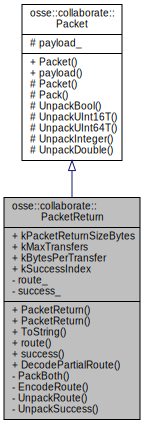
\includegraphics[width=226pt]{classosse_1_1collaborate_1_1_packet_return__inherit__graph}
\end{center}
\end{figure}
\subsubsection*{Public Types}
\begin{DoxyCompactItemize}
\item 
\mbox{\Hypertarget{classosse_1_1collaborate_1_1_packet_return_a6561da1547b84f40de85c6dea399116c}\label{classosse_1_1collaborate_1_1_packet_return_a6561da1547b84f40de85c6dea399116c}} 
typedef std\+::pair$<$ uint16\+\_\+t, uint64\+\_\+t $>$ \hyperlink{classosse_1_1collaborate_1_1_packet_return_a6561da1547b84f40de85c6dea399116c}{Event}
\begin{DoxyCompactList}\small\item\em A route containing node and transfer pairs. \end{DoxyCompactList}\item 
\mbox{\Hypertarget{classosse_1_1collaborate_1_1_packet_return_a56d5b319f0625cdabbfc4f6cbd01b002}\label{classosse_1_1collaborate_1_1_packet_return_a56d5b319f0625cdabbfc4f6cbd01b002}} 
typedef std\+::vector$<$ \hyperlink{classosse_1_1collaborate_1_1_packet_return_a6561da1547b84f40de85c6dea399116c}{Event} $>$ \hyperlink{classosse_1_1collaborate_1_1_packet_return_a56d5b319f0625cdabbfc4f6cbd01b002}{Partial\+Route}
\begin{DoxyCompactList}\small\item\em A partial route containing node and transfer pairs. \end{DoxyCompactList}\item 
\mbox{\Hypertarget{classosse_1_1collaborate_1_1_packet_return_a1c00d25b9e8d526be915c28b8ee0ba3b}\label{classosse_1_1collaborate_1_1_packet_return_a1c00d25b9e8d526be915c28b8ee0ba3b}} 
typedef std\+::array$<$ \hyperlink{classosse_1_1collaborate_1_1_packet_return_a6561da1547b84f40de85c6dea399116c}{Event}, \hyperlink{classosse_1_1collaborate_1_1_packet_return_a5e0eed3ac989888c4cc3ea04aa76ae32}{k\+Max\+Transfers} $>$ \hyperlink{classosse_1_1collaborate_1_1_packet_return_a1c00d25b9e8d526be915c28b8ee0ba3b}{Route}
\begin{DoxyCompactList}\small\item\em A route containing node and transfer pairs. \end{DoxyCompactList}\end{DoxyCompactItemize}
\subsubsection*{Public Member Functions}
\begin{DoxyCompactItemize}
\item 
\hyperlink{classosse_1_1collaborate_1_1_packet_return_a09a26d47a8b30c5f7002ca8e4b8bb89a}{Packet\+Return} (const std\+::vector$<$ uint8\+\_\+t $>$ \&\+\_\+payload)
\begin{DoxyCompactList}\small\item\em Constructor from payload. \end{DoxyCompactList}\item 
\hyperlink{classosse_1_1collaborate_1_1_packet_return_aa98e41d208d00cd972125b63f5fcf8b5}{Packet\+Return} (const \hyperlink{classosse_1_1collaborate_1_1_packet_return_a56d5b319f0625cdabbfc4f6cbd01b002}{Partial\+Route} \&\+\_\+partial\+\_\+route, const std\+::pair$<$ bool, uint16\+\_\+t $>$ \&\+\_\+success)
\begin{DoxyCompactList}\small\item\em Constructor from data members. \end{DoxyCompactList}\item 
std\+::string \hyperlink{classosse_1_1collaborate_1_1_packet_return_a415e0fd114b2460f62a6800023dafc0a}{To\+String} () const
\begin{DoxyCompactList}\small\item\em Converts the packet to a string. \end{DoxyCompactList}\item 
const \hyperlink{classosse_1_1collaborate_1_1_packet_return_a1c00d25b9e8d526be915c28b8ee0ba3b}{Route} \& \hyperlink{classosse_1_1collaborate_1_1_packet_return_a7022bd230981dc2b8424b3ff180f9ef4}{route} () const
\begin{DoxyCompactList}\small\item\em Gets route. \end{DoxyCompactList}\item 
const std\+::pair$<$ bool, uint16\+\_\+t $>$ \& \hyperlink{classosse_1_1collaborate_1_1_packet_return_ac6b2ab10694bac5f89cf829e34742345}{success} () const
\begin{DoxyCompactList}\small\item\em Gets success. \end{DoxyCompactList}\item 
\hyperlink{classosse_1_1collaborate_1_1_packet_return_a56d5b319f0625cdabbfc4f6cbd01b002}{Partial\+Route} \hyperlink{classosse_1_1collaborate_1_1_packet_return_a2534afa0446ef8f4dbe9c051607e55d7}{Decode\+Partial\+Route} ()
\begin{DoxyCompactList}\small\item\em Decodes the route into a standard vector. \end{DoxyCompactList}\end{DoxyCompactItemize}
\subsubsection*{Static Public Attributes}
\begin{DoxyCompactItemize}
\item 
\mbox{\Hypertarget{classosse_1_1collaborate_1_1_packet_return_ac4c8213599bd47f85d83b85f27e2d24a}\label{classosse_1_1collaborate_1_1_packet_return_ac4c8213599bd47f85d83b85f27e2d24a}} 
static constexpr int \hyperlink{classosse_1_1collaborate_1_1_packet_return_ac4c8213599bd47f85d83b85f27e2d24a}{k\+Packet\+Return\+Size\+Bytes} = 303
\begin{DoxyCompactList}\small\item\em The size (bytes) \end{DoxyCompactList}\item 
\mbox{\Hypertarget{classosse_1_1collaborate_1_1_packet_return_a5e0eed3ac989888c4cc3ea04aa76ae32}\label{classosse_1_1collaborate_1_1_packet_return_a5e0eed3ac989888c4cc3ea04aa76ae32}} 
static constexpr int \hyperlink{classosse_1_1collaborate_1_1_packet_return_a5e0eed3ac989888c4cc3ea04aa76ae32}{k\+Max\+Transfers} = 30
\begin{DoxyCompactList}\small\item\em The maximum size of a route. \end{DoxyCompactList}\item 
\mbox{\Hypertarget{classosse_1_1collaborate_1_1_packet_return_a2672dc70431ab3c8933c6876bb1bdd83}\label{classosse_1_1collaborate_1_1_packet_return_a2672dc70431ab3c8933c6876bb1bdd83}} 
static constexpr int \hyperlink{classosse_1_1collaborate_1_1_packet_return_a2672dc70431ab3c8933c6876bb1bdd83}{k\+Bytes\+Per\+Transfer} = 10
\begin{DoxyCompactList}\small\item\em The number of bytes per transfer. \end{DoxyCompactList}\item 
\mbox{\Hypertarget{classosse_1_1collaborate_1_1_packet_return_af116129fe59660a284a1dc07c00e25d6}\label{classosse_1_1collaborate_1_1_packet_return_af116129fe59660a284a1dc07c00e25d6}} 
static constexpr int \hyperlink{classosse_1_1collaborate_1_1_packet_return_af116129fe59660a284a1dc07c00e25d6}{k\+Success\+Index} = \hyperlink{classosse_1_1collaborate_1_1_packet_return_a5e0eed3ac989888c4cc3ea04aa76ae32}{k\+Max\+Transfers} $\ast$ \hyperlink{classosse_1_1collaborate_1_1_packet_return_a2672dc70431ab3c8933c6876bb1bdd83}{k\+Bytes\+Per\+Transfer}
\begin{DoxyCompactList}\small\item\em The index of the event. \end{DoxyCompactList}\end{DoxyCompactItemize}
\subsubsection*{Private Member Functions}
\begin{DoxyCompactItemize}
\item 
std\+::vector$<$ uint8\+\_\+t $>$ \hyperlink{classosse_1_1collaborate_1_1_packet_return_a4e9f99f25411e60d84bd08940496efec}{Pack\+Both} (const \hyperlink{classosse_1_1collaborate_1_1_packet_return_a56d5b319f0625cdabbfc4f6cbd01b002}{Partial\+Route} \&\+\_\+partial\+\_\+route, const std\+::pair$<$ bool, uint16\+\_\+t $>$ \&\+\_\+success) const
\begin{DoxyCompactList}\small\item\em Packs member elements into a payload. \end{DoxyCompactList}\item 
\hyperlink{classosse_1_1collaborate_1_1_packet_return_a1c00d25b9e8d526be915c28b8ee0ba3b}{Route} \hyperlink{classosse_1_1collaborate_1_1_packet_return_a8b63f26c2503ba37b133aab0da1e718c}{Encode\+Route} (const \hyperlink{classosse_1_1collaborate_1_1_packet_return_a56d5b319f0625cdabbfc4f6cbd01b002}{Partial\+Route} \&\+\_\+partial\+\_\+route) const
\begin{DoxyCompactList}\small\item\em Translates a vector to an array. \end{DoxyCompactList}\item 
\hyperlink{classosse_1_1collaborate_1_1_packet_return_a1c00d25b9e8d526be915c28b8ee0ba3b}{Route} \hyperlink{classosse_1_1collaborate_1_1_packet_return_ae430891dd740edab4984a0279816797c}{Unpack\+Route} (const std\+::vector$<$ uint8\+\_\+t $>$ \&\+\_\+payload) const
\begin{DoxyCompactList}\small\item\em Unpacks the route from the payload. \end{DoxyCompactList}\item 
std\+::pair$<$ bool, uint16\+\_\+t $>$ \hyperlink{classosse_1_1collaborate_1_1_packet_return_a89a3e35f9caf7dc3cfe13533ae8b538f}{Unpack\+Success} (const std\+::vector$<$ uint8\+\_\+t $>$ \&\+\_\+payload) const
\begin{DoxyCompactList}\small\item\em Unpacks the success from the payload. \end{DoxyCompactList}\end{DoxyCompactItemize}
\subsubsection*{Private Attributes}
\begin{DoxyCompactItemize}
\item 
\mbox{\Hypertarget{classosse_1_1collaborate_1_1_packet_return_a57c61ee6e1ae3b9bf876b85f16918a92}\label{classosse_1_1collaborate_1_1_packet_return_a57c61ee6e1ae3b9bf876b85f16918a92}} 
\hyperlink{classosse_1_1collaborate_1_1_packet_return_a1c00d25b9e8d526be915c28b8ee0ba3b}{Route} \hyperlink{classosse_1_1collaborate_1_1_packet_return_a57c61ee6e1ae3b9bf876b85f16918a92}{route\+\_\+}
\begin{DoxyCompactList}\small\item\em Route containing individual transfer. \end{DoxyCompactList}\item 
\mbox{\Hypertarget{classosse_1_1collaborate_1_1_packet_return_aaa6dd0adedb9734bc5a17f06b0702d38}\label{classosse_1_1collaborate_1_1_packet_return_aaa6dd0adedb9734bc5a17f06b0702d38}} 
std\+::pair$<$ bool, uint16\+\_\+t $>$ \hyperlink{classosse_1_1collaborate_1_1_packet_return_aaa6dd0adedb9734bc5a17f06b0702d38}{success\+\_\+}
\begin{DoxyCompactList}\small\item\em Whether a measurements exceed the desired threshold. \end{DoxyCompactList}\end{DoxyCompactItemize}
\subsubsection*{Additional Inherited Members}


\subsubsection{Detailed Description}
A packet of return data. 

\subsubsection{Constructor \& Destructor Documentation}
\mbox{\Hypertarget{classosse_1_1collaborate_1_1_packet_return_a09a26d47a8b30c5f7002ca8e4b8bb89a}\label{classosse_1_1collaborate_1_1_packet_return_a09a26d47a8b30c5f7002ca8e4b8bb89a}} 
\index{osse\+::collaborate\+::\+Packet\+Return@{osse\+::collaborate\+::\+Packet\+Return}!Packet\+Return@{Packet\+Return}}
\index{Packet\+Return@{Packet\+Return}!osse\+::collaborate\+::\+Packet\+Return@{osse\+::collaborate\+::\+Packet\+Return}}
\paragraph{\texorpdfstring{Packet\+Return()}{PacketReturn()}\hspace{0.1cm}{\footnotesize\ttfamily [1/2]}}
{\footnotesize\ttfamily osse\+::collaborate\+::\+Packet\+Return\+::\+Packet\+Return (\begin{DoxyParamCaption}\item[{const std\+::vector$<$ uint8\+\_\+t $>$ \&}]{\+\_\+payload }\end{DoxyParamCaption})\hspace{0.3cm}{\ttfamily [explicit]}}



Constructor from payload. 


\begin{DoxyParams}[1]{Parameters}
\mbox{\tt in}  & {\em \+\_\+payload} & Payload \\
\hline
\end{DoxyParams}
\mbox{\Hypertarget{classosse_1_1collaborate_1_1_packet_return_aa98e41d208d00cd972125b63f5fcf8b5}\label{classosse_1_1collaborate_1_1_packet_return_aa98e41d208d00cd972125b63f5fcf8b5}} 
\index{osse\+::collaborate\+::\+Packet\+Return@{osse\+::collaborate\+::\+Packet\+Return}!Packet\+Return@{Packet\+Return}}
\index{Packet\+Return@{Packet\+Return}!osse\+::collaborate\+::\+Packet\+Return@{osse\+::collaborate\+::\+Packet\+Return}}
\paragraph{\texorpdfstring{Packet\+Return()}{PacketReturn()}\hspace{0.1cm}{\footnotesize\ttfamily [2/2]}}
{\footnotesize\ttfamily osse\+::collaborate\+::\+Packet\+Return\+::\+Packet\+Return (\begin{DoxyParamCaption}\item[{const \hyperlink{classosse_1_1collaborate_1_1_packet_return_a56d5b319f0625cdabbfc4f6cbd01b002}{Partial\+Route} \&}]{\+\_\+partial\+\_\+route,  }\item[{const std\+::pair$<$ bool, uint16\+\_\+t $>$ \&}]{\+\_\+success }\end{DoxyParamCaption})}



Constructor from data members. 


\begin{DoxyParams}[1]{Parameters}
\mbox{\tt in}  & {\em \+\_\+partial\+\_\+route} & Route \\
\hline
\mbox{\tt in}  & {\em \+\_\+success} & Whether the threshold was exceeded \\
\hline
\end{DoxyParams}


\subsubsection{Member Function Documentation}
\mbox{\Hypertarget{classosse_1_1collaborate_1_1_packet_return_a2534afa0446ef8f4dbe9c051607e55d7}\label{classosse_1_1collaborate_1_1_packet_return_a2534afa0446ef8f4dbe9c051607e55d7}} 
\index{osse\+::collaborate\+::\+Packet\+Return@{osse\+::collaborate\+::\+Packet\+Return}!Decode\+Partial\+Route@{Decode\+Partial\+Route}}
\index{Decode\+Partial\+Route@{Decode\+Partial\+Route}!osse\+::collaborate\+::\+Packet\+Return@{osse\+::collaborate\+::\+Packet\+Return}}
\paragraph{\texorpdfstring{Decode\+Partial\+Route()}{DecodePartialRoute()}}
{\footnotesize\ttfamily \hyperlink{classosse_1_1collaborate_1_1_packet_return_a56d5b319f0625cdabbfc4f6cbd01b002}{Packet\+Return\+::\+Partial\+Route} osse\+::collaborate\+::\+Packet\+Return\+::\+Decode\+Partial\+Route (\begin{DoxyParamCaption}{ }\end{DoxyParamCaption})}



Decodes the route into a standard vector. 

\begin{DoxyReturn}{Returns}
Route as a vector 
\end{DoxyReturn}
\mbox{\Hypertarget{classosse_1_1collaborate_1_1_packet_return_a8b63f26c2503ba37b133aab0da1e718c}\label{classosse_1_1collaborate_1_1_packet_return_a8b63f26c2503ba37b133aab0da1e718c}} 
\index{osse\+::collaborate\+::\+Packet\+Return@{osse\+::collaborate\+::\+Packet\+Return}!Encode\+Route@{Encode\+Route}}
\index{Encode\+Route@{Encode\+Route}!osse\+::collaborate\+::\+Packet\+Return@{osse\+::collaborate\+::\+Packet\+Return}}
\paragraph{\texorpdfstring{Encode\+Route()}{EncodeRoute()}}
{\footnotesize\ttfamily \hyperlink{classosse_1_1collaborate_1_1_packet_return_a1c00d25b9e8d526be915c28b8ee0ba3b}{Packet\+Return\+::\+Route} osse\+::collaborate\+::\+Packet\+Return\+::\+Encode\+Route (\begin{DoxyParamCaption}\item[{const \hyperlink{classosse_1_1collaborate_1_1_packet_return_a56d5b319f0625cdabbfc4f6cbd01b002}{Partial\+Route} \&}]{\+\_\+partial\+\_\+route }\end{DoxyParamCaption}) const\hspace{0.3cm}{\ttfamily [private]}}



Translates a vector to an array. 


\begin{DoxyParams}[1]{Parameters}
\mbox{\tt in}  & {\em \+\_\+partial\+\_\+route} & Route as a vector \\
\hline
\end{DoxyParams}
\begin{DoxyReturn}{Returns}
Route (array) 
\end{DoxyReturn}
\mbox{\Hypertarget{classosse_1_1collaborate_1_1_packet_return_a4e9f99f25411e60d84bd08940496efec}\label{classosse_1_1collaborate_1_1_packet_return_a4e9f99f25411e60d84bd08940496efec}} 
\index{osse\+::collaborate\+::\+Packet\+Return@{osse\+::collaborate\+::\+Packet\+Return}!Pack\+Both@{Pack\+Both}}
\index{Pack\+Both@{Pack\+Both}!osse\+::collaborate\+::\+Packet\+Return@{osse\+::collaborate\+::\+Packet\+Return}}
\paragraph{\texorpdfstring{Pack\+Both()}{PackBoth()}}
{\footnotesize\ttfamily std\+::vector$<$ uint8\+\_\+t $>$ osse\+::collaborate\+::\+Packet\+Return\+::\+Pack\+Both (\begin{DoxyParamCaption}\item[{const \hyperlink{classosse_1_1collaborate_1_1_packet_return_a56d5b319f0625cdabbfc4f6cbd01b002}{Partial\+Route} \&}]{\+\_\+partial\+\_\+route,  }\item[{const std\+::pair$<$ bool, uint16\+\_\+t $>$ \&}]{\+\_\+success }\end{DoxyParamCaption}) const\hspace{0.3cm}{\ttfamily [private]}}



Packs member elements into a payload. 


\begin{DoxyParams}[1]{Parameters}
\mbox{\tt in}  & {\em \+\_\+partial\+\_\+route} & Partial route \\
\hline
\mbox{\tt in}  & {\em \+\_\+success} & Success \\
\hline
\end{DoxyParams}
\begin{DoxyReturn}{Returns}
Payload 
\end{DoxyReturn}
\mbox{\Hypertarget{classosse_1_1collaborate_1_1_packet_return_a7022bd230981dc2b8424b3ff180f9ef4}\label{classosse_1_1collaborate_1_1_packet_return_a7022bd230981dc2b8424b3ff180f9ef4}} 
\index{osse\+::collaborate\+::\+Packet\+Return@{osse\+::collaborate\+::\+Packet\+Return}!route@{route}}
\index{route@{route}!osse\+::collaborate\+::\+Packet\+Return@{osse\+::collaborate\+::\+Packet\+Return}}
\paragraph{\texorpdfstring{route()}{route()}}
{\footnotesize\ttfamily const \hyperlink{classosse_1_1collaborate_1_1_packet_return_a1c00d25b9e8d526be915c28b8ee0ba3b}{Route}\& osse\+::collaborate\+::\+Packet\+Return\+::route (\begin{DoxyParamCaption}{ }\end{DoxyParamCaption}) const\hspace{0.3cm}{\ttfamily [inline]}}



Gets route. 

\begin{DoxyReturn}{Returns}
route\+\_\+ Route 
\end{DoxyReturn}
\mbox{\Hypertarget{classosse_1_1collaborate_1_1_packet_return_ac6b2ab10694bac5f89cf829e34742345}\label{classosse_1_1collaborate_1_1_packet_return_ac6b2ab10694bac5f89cf829e34742345}} 
\index{osse\+::collaborate\+::\+Packet\+Return@{osse\+::collaborate\+::\+Packet\+Return}!success@{success}}
\index{success@{success}!osse\+::collaborate\+::\+Packet\+Return@{osse\+::collaborate\+::\+Packet\+Return}}
\paragraph{\texorpdfstring{success()}{success()}}
{\footnotesize\ttfamily const std\+::pair$<$bool, uint16\+\_\+t$>$\& osse\+::collaborate\+::\+Packet\+Return\+::success (\begin{DoxyParamCaption}{ }\end{DoxyParamCaption}) const\hspace{0.3cm}{\ttfamily [inline]}}



Gets success. 

\begin{DoxyReturn}{Returns}
success\+\_\+ Success 
\end{DoxyReturn}
\mbox{\Hypertarget{classosse_1_1collaborate_1_1_packet_return_a415e0fd114b2460f62a6800023dafc0a}\label{classosse_1_1collaborate_1_1_packet_return_a415e0fd114b2460f62a6800023dafc0a}} 
\index{osse\+::collaborate\+::\+Packet\+Return@{osse\+::collaborate\+::\+Packet\+Return}!To\+String@{To\+String}}
\index{To\+String@{To\+String}!osse\+::collaborate\+::\+Packet\+Return@{osse\+::collaborate\+::\+Packet\+Return}}
\paragraph{\texorpdfstring{To\+String()}{ToString()}}
{\footnotesize\ttfamily std\+::string osse\+::collaborate\+::\+Packet\+Return\+::\+To\+String (\begin{DoxyParamCaption}{ }\end{DoxyParamCaption}) const}



Converts the packet to a string. 

\begin{DoxyReturn}{Returns}
\hyperlink{classosse_1_1collaborate_1_1_packet}{Packet} as a string 
\end{DoxyReturn}
\mbox{\Hypertarget{classosse_1_1collaborate_1_1_packet_return_ae430891dd740edab4984a0279816797c}\label{classosse_1_1collaborate_1_1_packet_return_ae430891dd740edab4984a0279816797c}} 
\index{osse\+::collaborate\+::\+Packet\+Return@{osse\+::collaborate\+::\+Packet\+Return}!Unpack\+Route@{Unpack\+Route}}
\index{Unpack\+Route@{Unpack\+Route}!osse\+::collaborate\+::\+Packet\+Return@{osse\+::collaborate\+::\+Packet\+Return}}
\paragraph{\texorpdfstring{Unpack\+Route()}{UnpackRoute()}}
{\footnotesize\ttfamily \hyperlink{classosse_1_1collaborate_1_1_packet_return_a1c00d25b9e8d526be915c28b8ee0ba3b}{Packet\+Return\+::\+Route} osse\+::collaborate\+::\+Packet\+Return\+::\+Unpack\+Route (\begin{DoxyParamCaption}\item[{const std\+::vector$<$ uint8\+\_\+t $>$ \&}]{\+\_\+payload }\end{DoxyParamCaption}) const\hspace{0.3cm}{\ttfamily [private]}}



Unpacks the route from the payload. 


\begin{DoxyParams}[1]{Parameters}
\mbox{\tt in}  & {\em \+\_\+payload} & Payload \\
\hline
\end{DoxyParams}
\begin{DoxyReturn}{Returns}
Route (array) 
\end{DoxyReturn}
\mbox{\Hypertarget{classosse_1_1collaborate_1_1_packet_return_a89a3e35f9caf7dc3cfe13533ae8b538f}\label{classosse_1_1collaborate_1_1_packet_return_a89a3e35f9caf7dc3cfe13533ae8b538f}} 
\index{osse\+::collaborate\+::\+Packet\+Return@{osse\+::collaborate\+::\+Packet\+Return}!Unpack\+Success@{Unpack\+Success}}
\index{Unpack\+Success@{Unpack\+Success}!osse\+::collaborate\+::\+Packet\+Return@{osse\+::collaborate\+::\+Packet\+Return}}
\paragraph{\texorpdfstring{Unpack\+Success()}{UnpackSuccess()}}
{\footnotesize\ttfamily std\+::pair$<$ bool, uint16\+\_\+t $>$ osse\+::collaborate\+::\+Packet\+Return\+::\+Unpack\+Success (\begin{DoxyParamCaption}\item[{const std\+::vector$<$ uint8\+\_\+t $>$ \&}]{\+\_\+payload }\end{DoxyParamCaption}) const\hspace{0.3cm}{\ttfamily [private]}}



Unpacks the success from the payload. 


\begin{DoxyParams}[1]{Parameters}
\mbox{\tt in}  & {\em \+\_\+payload} & Payload \\
\hline
\end{DoxyParams}
\begin{DoxyReturn}{Returns}
Success 
\end{DoxyReturn}


The documentation for this class was generated from the following files\+:\begin{DoxyCompactItemize}
\item 
libs/collaborate/include/collaborate/packet\+\_\+return.\+h\item 
libs/collaborate/src/packet\+\_\+return.\+cpp\end{DoxyCompactItemize}

\hypertarget{classosse_1_1collaborate_1_1_packet}{}\subsection{osse\+:\+:collaborate\+:\+:Packet Class Reference}
\label{classosse_1_1collaborate_1_1_packet}\index{osse\+::collaborate\+::\+Packet@{osse\+::collaborate\+::\+Packet}}


An abstract container for information.  




{\ttfamily \#include $<$packet.\+h$>$}



Inheritance diagram for osse\+:\+:collaborate\+:\+:Packet\+:
\nopagebreak
\begin{figure}[H]
\begin{center}
\leavevmode
\includegraphics[height=550pt]{classosse_1_1collaborate_1_1_packet__inherit__graph}
\end{center}
\end{figure}
\subsubsection*{Public Member Functions}
\begin{DoxyCompactItemize}
\item 
\mbox{\Hypertarget{classosse_1_1collaborate_1_1_packet_aecb3018048e1845ea9e45dcd008cc0df}\label{classosse_1_1collaborate_1_1_packet_aecb3018048e1845ea9e45dcd008cc0df}} 
\hyperlink{classosse_1_1collaborate_1_1_packet_aecb3018048e1845ea9e45dcd008cc0df}{Packet} ()
\begin{DoxyCompactList}\small\item\em Default Constructor. \end{DoxyCompactList}\item 
const std\+::vector$<$ uint8\+\_\+t $>$ \& \hyperlink{classosse_1_1collaborate_1_1_packet_a6034dd26382166bf4feeed7cecda3e54}{payload} () const
\begin{DoxyCompactList}\small\item\em Get payload. \end{DoxyCompactList}\end{DoxyCompactItemize}
\subsubsection*{Protected Member Functions}
\begin{DoxyCompactItemize}
\item 
\hyperlink{classosse_1_1collaborate_1_1_packet_a83e5d92a626c5adb0958c0faf7bbbf87}{Packet} (const std\+::vector$<$ uint8\+\_\+t $>$ \&\+\_\+payload)
\begin{DoxyCompactList}\small\item\em Default Constructor. \end{DoxyCompactList}\item 
{\footnotesize template$<$class T $>$ }\\void \hyperlink{classosse_1_1collaborate_1_1_packet_a7ebfc5903ba6bf302e2f4a33340e7155}{Pack} (const T \&\+\_\+value, std\+::vector$<$ uint8\+\_\+t $>$ $\ast$\+\_\+payload) const
\begin{DoxyCompactList}\small\item\em Inserts a generic value into the payload. \end{DoxyCompactList}\item 
bool \hyperlink{classosse_1_1collaborate_1_1_packet_acf78e5e563ba07643fb1969dc332b1fb}{Unpack\+Bool} (const std\+::vector$<$ uint8\+\_\+t $>$ \&\+\_\+payload, const uint16\+\_\+t \&\+\_\+index) const
\begin{DoxyCompactList}\small\item\em Unpacks a boolean value from the \+\_\+payload. \end{DoxyCompactList}\item 
uint16\+\_\+t \hyperlink{classosse_1_1collaborate_1_1_packet_a454166985d9b63b553cb6174417c4dde}{Unpack\+U\+Int16T} (const std\+::vector$<$ uint8\+\_\+t $>$ \&\+\_\+payload, const uint16\+\_\+t \&\+\_\+index) const
\begin{DoxyCompactList}\small\item\em Unpacks a short unsigned integer from the \+\_\+payload. \end{DoxyCompactList}\item 
uint64\+\_\+t \hyperlink{classosse_1_1collaborate_1_1_packet_ab84b122670543d85df644041129568df}{Unpack\+U\+Int64T} (const std\+::vector$<$ uint8\+\_\+t $>$ \&\+\_\+payload, const uint16\+\_\+t \&\+\_\+index) const
\begin{DoxyCompactList}\small\item\em Unpacks a long unsigned integer from the payload. \end{DoxyCompactList}\item 
int \hyperlink{classosse_1_1collaborate_1_1_packet_a7c786b41b594b51377b0a70ce3a61259}{Unpack\+Integer} (const std\+::vector$<$ uint8\+\_\+t $>$ \&\+\_\+payload, const uint16\+\_\+t \&\+\_\+index) const
\begin{DoxyCompactList}\small\item\em Unpacks an integer from the payload. \end{DoxyCompactList}\item 
double \hyperlink{classosse_1_1collaborate_1_1_packet_aa7678be22b45d54b28f1b85594638d60}{Unpack\+Double} (const std\+::vector$<$ uint8\+\_\+t $>$ \&\+\_\+payload, const uint16\+\_\+t \&\+\_\+index) const
\begin{DoxyCompactList}\small\item\em Unpacks a double from the payload. \end{DoxyCompactList}\end{DoxyCompactItemize}
\subsubsection*{Protected Attributes}
\begin{DoxyCompactItemize}
\item 
\mbox{\Hypertarget{classosse_1_1collaborate_1_1_packet_a1917bbaba5a0fb4757947d2626287410}\label{classosse_1_1collaborate_1_1_packet_a1917bbaba5a0fb4757947d2626287410}} 
std\+::vector$<$ uint8\+\_\+t $>$ \hyperlink{classosse_1_1collaborate_1_1_packet_a1917bbaba5a0fb4757947d2626287410}{payload\+\_\+}
\begin{DoxyCompactList}\small\item\em Data contents (a vector of bytes) \end{DoxyCompactList}\end{DoxyCompactItemize}


\subsubsection{Detailed Description}
An abstract container for information. 

\subsubsection{Constructor \& Destructor Documentation}
\mbox{\Hypertarget{classosse_1_1collaborate_1_1_packet_a83e5d92a626c5adb0958c0faf7bbbf87}\label{classosse_1_1collaborate_1_1_packet_a83e5d92a626c5adb0958c0faf7bbbf87}} 
\index{osse\+::collaborate\+::\+Packet@{osse\+::collaborate\+::\+Packet}!Packet@{Packet}}
\index{Packet@{Packet}!osse\+::collaborate\+::\+Packet@{osse\+::collaborate\+::\+Packet}}
\paragraph{\texorpdfstring{Packet()}{Packet()}}
{\footnotesize\ttfamily osse\+::collaborate\+::\+Packet\+::\+Packet (\begin{DoxyParamCaption}\item[{const std\+::vector$<$ uint8\+\_\+t $>$ \&}]{\+\_\+payload }\end{DoxyParamCaption})\hspace{0.3cm}{\ttfamily [explicit]}, {\ttfamily [protected]}}



Default Constructor. 


\begin{DoxyParams}[1]{Parameters}
\mbox{\tt in}  & {\em \+\_\+payload} & The payload \\
\hline
\end{DoxyParams}


\subsubsection{Member Function Documentation}
\mbox{\Hypertarget{classosse_1_1collaborate_1_1_packet_a7ebfc5903ba6bf302e2f4a33340e7155}\label{classosse_1_1collaborate_1_1_packet_a7ebfc5903ba6bf302e2f4a33340e7155}} 
\index{osse\+::collaborate\+::\+Packet@{osse\+::collaborate\+::\+Packet}!Pack@{Pack}}
\index{Pack@{Pack}!osse\+::collaborate\+::\+Packet@{osse\+::collaborate\+::\+Packet}}
\paragraph{\texorpdfstring{Pack()}{Pack()}}
{\footnotesize\ttfamily template$<$class T $>$ \\
void osse\+::collaborate\+::\+Packet\+::\+Pack (\begin{DoxyParamCaption}\item[{const T \&}]{\+\_\+value,  }\item[{std\+::vector$<$ uint8\+\_\+t $>$ $\ast$}]{\+\_\+payload }\end{DoxyParamCaption}) const\hspace{0.3cm}{\ttfamily [inline]}, {\ttfamily [protected]}}



Inserts a generic value into the payload. 


\begin{DoxyParams}[1]{Parameters}
\mbox{\tt in}  & {\em \+\_\+value} & Value \\
\hline
\mbox{\tt in}  & {\em \+\_\+payload} & Payload \\
\hline
\end{DoxyParams}
\mbox{\Hypertarget{classosse_1_1collaborate_1_1_packet_a6034dd26382166bf4feeed7cecda3e54}\label{classosse_1_1collaborate_1_1_packet_a6034dd26382166bf4feeed7cecda3e54}} 
\index{osse\+::collaborate\+::\+Packet@{osse\+::collaborate\+::\+Packet}!payload@{payload}}
\index{payload@{payload}!osse\+::collaborate\+::\+Packet@{osse\+::collaborate\+::\+Packet}}
\paragraph{\texorpdfstring{payload()}{payload()}}
{\footnotesize\ttfamily const std\+::vector$<$uint8\+\_\+t$>$\& osse\+::collaborate\+::\+Packet\+::payload (\begin{DoxyParamCaption}{ }\end{DoxyParamCaption}) const\hspace{0.3cm}{\ttfamily [inline]}}



Get payload. 

\begin{DoxyReturn}{Returns}
payload\+\_\+ Payload 
\end{DoxyReturn}
\mbox{\Hypertarget{classosse_1_1collaborate_1_1_packet_acf78e5e563ba07643fb1969dc332b1fb}\label{classosse_1_1collaborate_1_1_packet_acf78e5e563ba07643fb1969dc332b1fb}} 
\index{osse\+::collaborate\+::\+Packet@{osse\+::collaborate\+::\+Packet}!Unpack\+Bool@{Unpack\+Bool}}
\index{Unpack\+Bool@{Unpack\+Bool}!osse\+::collaborate\+::\+Packet@{osse\+::collaborate\+::\+Packet}}
\paragraph{\texorpdfstring{Unpack\+Bool()}{UnpackBool()}}
{\footnotesize\ttfamily bool osse\+::collaborate\+::\+Packet\+::\+Unpack\+Bool (\begin{DoxyParamCaption}\item[{const std\+::vector$<$ uint8\+\_\+t $>$ \&}]{\+\_\+payload,  }\item[{const uint16\+\_\+t \&}]{\+\_\+index }\end{DoxyParamCaption}) const\hspace{0.3cm}{\ttfamily [protected]}}



Unpacks a boolean value from the \+\_\+payload. 


\begin{DoxyParams}[1]{Parameters}
\mbox{\tt in}  & {\em \+\_\+payload} & Payload \\
\hline
\mbox{\tt in}  & {\em \+\_\+index} & Index in the payload vector \\
\hline
\end{DoxyParams}
\begin{DoxyReturn}{Returns}
Unpacked boolean value 
\end{DoxyReturn}
\mbox{\Hypertarget{classosse_1_1collaborate_1_1_packet_aa7678be22b45d54b28f1b85594638d60}\label{classosse_1_1collaborate_1_1_packet_aa7678be22b45d54b28f1b85594638d60}} 
\index{osse\+::collaborate\+::\+Packet@{osse\+::collaborate\+::\+Packet}!Unpack\+Double@{Unpack\+Double}}
\index{Unpack\+Double@{Unpack\+Double}!osse\+::collaborate\+::\+Packet@{osse\+::collaborate\+::\+Packet}}
\paragraph{\texorpdfstring{Unpack\+Double()}{UnpackDouble()}}
{\footnotesize\ttfamily double osse\+::collaborate\+::\+Packet\+::\+Unpack\+Double (\begin{DoxyParamCaption}\item[{const std\+::vector$<$ uint8\+\_\+t $>$ \&}]{\+\_\+payload,  }\item[{const uint16\+\_\+t \&}]{\+\_\+index }\end{DoxyParamCaption}) const\hspace{0.3cm}{\ttfamily [protected]}}



Unpacks a double from the payload. 


\begin{DoxyParams}[1]{Parameters}
\mbox{\tt in}  & {\em \+\_\+payload} & Payload \\
\hline
\mbox{\tt in}  & {\em \+\_\+index} & Index in the payload vector \\
\hline
\end{DoxyParams}
\begin{DoxyReturn}{Returns}
Unpacked double 
\end{DoxyReturn}
\mbox{\Hypertarget{classosse_1_1collaborate_1_1_packet_a7c786b41b594b51377b0a70ce3a61259}\label{classosse_1_1collaborate_1_1_packet_a7c786b41b594b51377b0a70ce3a61259}} 
\index{osse\+::collaborate\+::\+Packet@{osse\+::collaborate\+::\+Packet}!Unpack\+Integer@{Unpack\+Integer}}
\index{Unpack\+Integer@{Unpack\+Integer}!osse\+::collaborate\+::\+Packet@{osse\+::collaborate\+::\+Packet}}
\paragraph{\texorpdfstring{Unpack\+Integer()}{UnpackInteger()}}
{\footnotesize\ttfamily int osse\+::collaborate\+::\+Packet\+::\+Unpack\+Integer (\begin{DoxyParamCaption}\item[{const std\+::vector$<$ uint8\+\_\+t $>$ \&}]{\+\_\+payload,  }\item[{const uint16\+\_\+t \&}]{\+\_\+index }\end{DoxyParamCaption}) const\hspace{0.3cm}{\ttfamily [protected]}}



Unpacks an integer from the payload. 


\begin{DoxyParams}[1]{Parameters}
\mbox{\tt in}  & {\em \+\_\+payload} & Payload \\
\hline
\mbox{\tt in}  & {\em \+\_\+index} & Index in the payload vector \\
\hline
\end{DoxyParams}
\begin{DoxyReturn}{Returns}
Unpacked integer 
\end{DoxyReturn}
\mbox{\Hypertarget{classosse_1_1collaborate_1_1_packet_a454166985d9b63b553cb6174417c4dde}\label{classosse_1_1collaborate_1_1_packet_a454166985d9b63b553cb6174417c4dde}} 
\index{osse\+::collaborate\+::\+Packet@{osse\+::collaborate\+::\+Packet}!Unpack\+U\+Int16T@{Unpack\+U\+Int16T}}
\index{Unpack\+U\+Int16T@{Unpack\+U\+Int16T}!osse\+::collaborate\+::\+Packet@{osse\+::collaborate\+::\+Packet}}
\paragraph{\texorpdfstring{Unpack\+U\+Int16\+T()}{UnpackUInt16T()}}
{\footnotesize\ttfamily uint16\+\_\+t osse\+::collaborate\+::\+Packet\+::\+Unpack\+U\+Int16T (\begin{DoxyParamCaption}\item[{const std\+::vector$<$ uint8\+\_\+t $>$ \&}]{\+\_\+payload,  }\item[{const uint16\+\_\+t \&}]{\+\_\+index }\end{DoxyParamCaption}) const\hspace{0.3cm}{\ttfamily [protected]}}



Unpacks a short unsigned integer from the \+\_\+payload. 


\begin{DoxyParams}[1]{Parameters}
\mbox{\tt in}  & {\em \+\_\+payload} & Payload \\
\hline
\mbox{\tt in}  & {\em \+\_\+index} & Index in the payload vector \\
\hline
\end{DoxyParams}
\begin{DoxyReturn}{Returns}
Unpacked short unsigned integer 
\end{DoxyReturn}
\mbox{\Hypertarget{classosse_1_1collaborate_1_1_packet_ab84b122670543d85df644041129568df}\label{classosse_1_1collaborate_1_1_packet_ab84b122670543d85df644041129568df}} 
\index{osse\+::collaborate\+::\+Packet@{osse\+::collaborate\+::\+Packet}!Unpack\+U\+Int64T@{Unpack\+U\+Int64T}}
\index{Unpack\+U\+Int64T@{Unpack\+U\+Int64T}!osse\+::collaborate\+::\+Packet@{osse\+::collaborate\+::\+Packet}}
\paragraph{\texorpdfstring{Unpack\+U\+Int64\+T()}{UnpackUInt64T()}}
{\footnotesize\ttfamily uint64\+\_\+t osse\+::collaborate\+::\+Packet\+::\+Unpack\+U\+Int64T (\begin{DoxyParamCaption}\item[{const std\+::vector$<$ uint8\+\_\+t $>$ \&}]{\+\_\+payload,  }\item[{const uint16\+\_\+t \&}]{\+\_\+index }\end{DoxyParamCaption}) const\hspace{0.3cm}{\ttfamily [protected]}}



Unpacks a long unsigned integer from the payload. 


\begin{DoxyParams}[1]{Parameters}
\mbox{\tt in}  & {\em \+\_\+payload} & Payload \\
\hline
\mbox{\tt in}  & {\em \+\_\+index} & Index in the payload vector \\
\hline
\end{DoxyParams}
\begin{DoxyReturn}{Returns}
Unpacked long unsigned integer 
\end{DoxyReturn}


The documentation for this class was generated from the following files\+:\begin{DoxyCompactItemize}
\item 
libs/collaborate/include/collaborate/packet.\+h\item 
libs/collaborate/src/packet.\+cpp\end{DoxyCompactItemize}

\hypertarget{classosse_1_1collaborate_1_1_platform_earth}{}\subsection{osse\+:\+:collaborate\+:\+:Platform\+Earth Class Reference}
\label{classosse_1_1collaborate_1_1_platform_earth}\index{osse\+::collaborate\+::\+Platform\+Earth@{osse\+::collaborate\+::\+Platform\+Earth}}


Propogates the position of a stationary object on Earth\textquotesingle{}s surface.  




{\ttfamily \#include $<$platform\+\_\+earth.\+h$>$}



Inheritance diagram for osse\+:\+:collaborate\+:\+:Platform\+Earth\+:
\nopagebreak
\begin{figure}[H]
\begin{center}
\leavevmode
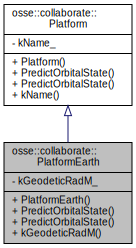
\includegraphics[width=208pt]{classosse_1_1collaborate_1_1_platform_earth__inherit__graph}
\end{center}
\end{figure}
\subsubsection*{Public Member Functions}
\begin{DoxyCompactItemize}
\item 
\hyperlink{classosse_1_1collaborate_1_1_platform_earth_afc5a80925b8a51fbdb93e0cc8eea3607}{Platform\+Earth} (const std\+::string \&\+\_\+name, const double \&\+\_\+latitude\+\_\+rad, const double \&\+\_\+longitude\+\_\+rad, const double \&\+\_\+altitude\+\_\+m)
\begin{DoxyCompactList}\small\item\em Constructor From L\+LH. \end{DoxyCompactList}\item 
\hyperlink{classosse_1_1collaborate_1_1_orbital_state}{Orbital\+State} \hyperlink{classosse_1_1collaborate_1_1_platform_earth_aff04ed83ab0ae2f7b3bcb1019588efcd}{Predict\+Orbital\+State} (const \hyperlink{classosse_1_1collaborate_1_1_simulation_clock}{Simulation\+Clock} \&\+\_\+clock, const uint64\+\_\+t \&\+\_\+time\+\_\+s) const
\begin{DoxyCompactList}\small\item\em Get the orbital\+\_\+state of an object using the current clock value. \end{DoxyCompactList}\item 
void \hyperlink{classosse_1_1collaborate_1_1_platform_earth_ab49f25fe5d37334918483cfdcef3471a}{Predict\+Orbital\+State} (const \hyperlink{classosse_1_1collaborate_1_1_simulation_clock}{Simulation\+Clock} \&\+\_\+clock, const uint64\+\_\+t \&\+\_\+time\+\_\+s, \hyperlink{classosse_1_1collaborate_1_1_orbital_state}{Orbital\+State} $\ast$\+\_\+orbital\+\_\+state) const
\begin{DoxyCompactList}\small\item\em Update the orbital\+\_\+state of an object the current clock time. \end{DoxyCompactList}\item 
const \hyperlink{classosse_1_1collaborate_1_1_geodetic}{Geodetic} \& \hyperlink{classosse_1_1collaborate_1_1_platform_earth_ac422459d6fb6cf713b52730f7e51f5b0}{k\+Geodetic\+RadM} () const
\begin{DoxyCompactList}\small\item\em Get geodetic position. \end{DoxyCompactList}\end{DoxyCompactItemize}
\subsubsection*{Private Attributes}
\begin{DoxyCompactItemize}
\item 
\mbox{\Hypertarget{classosse_1_1collaborate_1_1_platform_earth_ab79ec0de68f62f6355614bc3963cf44f}\label{classosse_1_1collaborate_1_1_platform_earth_ab79ec0de68f62f6355614bc3963cf44f}} 
const \hyperlink{classosse_1_1collaborate_1_1_geodetic}{Geodetic} \hyperlink{classosse_1_1collaborate_1_1_platform_earth_ab79ec0de68f62f6355614bc3963cf44f}{k\+Geodetic\+Rad\+M\+\_\+}
\begin{DoxyCompactList}\small\item\em \hyperlink{classosse_1_1collaborate_1_1_geodetic}{Geodetic} position. \end{DoxyCompactList}\end{DoxyCompactItemize}


\subsubsection{Detailed Description}
Propogates the position of a stationary object on Earth\textquotesingle{}s surface. 

\subsubsection{Constructor \& Destructor Documentation}
\mbox{\Hypertarget{classosse_1_1collaborate_1_1_platform_earth_afc5a80925b8a51fbdb93e0cc8eea3607}\label{classosse_1_1collaborate_1_1_platform_earth_afc5a80925b8a51fbdb93e0cc8eea3607}} 
\index{osse\+::collaborate\+::\+Platform\+Earth@{osse\+::collaborate\+::\+Platform\+Earth}!Platform\+Earth@{Platform\+Earth}}
\index{Platform\+Earth@{Platform\+Earth}!osse\+::collaborate\+::\+Platform\+Earth@{osse\+::collaborate\+::\+Platform\+Earth}}
\paragraph{\texorpdfstring{Platform\+Earth()}{PlatformEarth()}}
{\footnotesize\ttfamily osse\+::collaborate\+::\+Platform\+Earth\+::\+Platform\+Earth (\begin{DoxyParamCaption}\item[{const std\+::string \&}]{\+\_\+name,  }\item[{const double \&}]{\+\_\+latitude\+\_\+rad,  }\item[{const double \&}]{\+\_\+longitude\+\_\+rad,  }\item[{const double \&}]{\+\_\+altitude\+\_\+m }\end{DoxyParamCaption})}



Constructor From L\+LH. 


\begin{DoxyParams}[1]{Parameters}
\mbox{\tt in}  & {\em \+\_\+name} & Name of the platform \\
\hline
\mbox{\tt in}  & {\em \+\_\+latitude\+\_\+rad} & Latitude (radians) \\
\hline
\mbox{\tt in}  & {\em \+\_\+longitude\+\_\+rad} & Longitude (radians) \\
\hline
\mbox{\tt in}  & {\em \+\_\+altitude\+\_\+m} & Altitude (meters) \\
\hline
\end{DoxyParams}


\subsubsection{Member Function Documentation}
\mbox{\Hypertarget{classosse_1_1collaborate_1_1_platform_earth_ac422459d6fb6cf713b52730f7e51f5b0}\label{classosse_1_1collaborate_1_1_platform_earth_ac422459d6fb6cf713b52730f7e51f5b0}} 
\index{osse\+::collaborate\+::\+Platform\+Earth@{osse\+::collaborate\+::\+Platform\+Earth}!k\+Geodetic\+RadM@{k\+Geodetic\+RadM}}
\index{k\+Geodetic\+RadM@{k\+Geodetic\+RadM}!osse\+::collaborate\+::\+Platform\+Earth@{osse\+::collaborate\+::\+Platform\+Earth}}
\paragraph{\texorpdfstring{k\+Geodetic\+Rad\+M()}{kGeodeticRadM()}}
{\footnotesize\ttfamily const \hyperlink{classosse_1_1collaborate_1_1_geodetic}{Geodetic}\& osse\+::collaborate\+::\+Platform\+Earth\+::k\+Geodetic\+RadM (\begin{DoxyParamCaption}{ }\end{DoxyParamCaption}) const\hspace{0.3cm}{\ttfamily [inline]}}



Get geodetic position. 

\begin{DoxyReturn}{Returns}
geodetic\+\_\+ \hyperlink{classosse_1_1collaborate_1_1_geodetic}{Geodetic} position 
\end{DoxyReturn}
\mbox{\Hypertarget{classosse_1_1collaborate_1_1_platform_earth_aff04ed83ab0ae2f7b3bcb1019588efcd}\label{classosse_1_1collaborate_1_1_platform_earth_aff04ed83ab0ae2f7b3bcb1019588efcd}} 
\index{osse\+::collaborate\+::\+Platform\+Earth@{osse\+::collaborate\+::\+Platform\+Earth}!Predict\+Orbital\+State@{Predict\+Orbital\+State}}
\index{Predict\+Orbital\+State@{Predict\+Orbital\+State}!osse\+::collaborate\+::\+Platform\+Earth@{osse\+::collaborate\+::\+Platform\+Earth}}
\paragraph{\texorpdfstring{Predict\+Orbital\+State()}{PredictOrbitalState()}\hspace{0.1cm}{\footnotesize\ttfamily [1/2]}}
{\footnotesize\ttfamily \hyperlink{classosse_1_1collaborate_1_1_orbital_state}{Orbital\+State} osse\+::collaborate\+::\+Platform\+Earth\+::\+Predict\+Orbital\+State (\begin{DoxyParamCaption}\item[{const \hyperlink{classosse_1_1collaborate_1_1_simulation_clock}{Simulation\+Clock} \&}]{\+\_\+clock,  }\item[{const uint64\+\_\+t \&}]{\+\_\+time\+\_\+s }\end{DoxyParamCaption}) const\hspace{0.3cm}{\ttfamily [virtual]}}



Get the orbital\+\_\+state of an object using the current clock value. 


\begin{DoxyParams}[1]{Parameters}
\mbox{\tt in}  & {\em \+\_\+clock} & Simulation clock \\
\hline
\mbox{\tt in}  & {\em \+\_\+time\+\_\+s} & Time offset from the current time (seconds) \\
\hline
\end{DoxyParams}
\begin{DoxyReturn}{Returns}
orbital\+\_\+state \hyperlink{classosse_1_1collaborate_1_1_orbital_state}{Orbital\+State} of an obect at the specified time 
\end{DoxyReturn}


Implements \hyperlink{classosse_1_1collaborate_1_1_platform_ad7070fcb9d91b22f25dbe0211ba0cc73}{osse\+::collaborate\+::\+Platform}.

\mbox{\Hypertarget{classosse_1_1collaborate_1_1_platform_earth_ab49f25fe5d37334918483cfdcef3471a}\label{classosse_1_1collaborate_1_1_platform_earth_ab49f25fe5d37334918483cfdcef3471a}} 
\index{osse\+::collaborate\+::\+Platform\+Earth@{osse\+::collaborate\+::\+Platform\+Earth}!Predict\+Orbital\+State@{Predict\+Orbital\+State}}
\index{Predict\+Orbital\+State@{Predict\+Orbital\+State}!osse\+::collaborate\+::\+Platform\+Earth@{osse\+::collaborate\+::\+Platform\+Earth}}
\paragraph{\texorpdfstring{Predict\+Orbital\+State()}{PredictOrbitalState()}\hspace{0.1cm}{\footnotesize\ttfamily [2/2]}}
{\footnotesize\ttfamily void osse\+::collaborate\+::\+Platform\+Earth\+::\+Predict\+Orbital\+State (\begin{DoxyParamCaption}\item[{const \hyperlink{classosse_1_1collaborate_1_1_simulation_clock}{Simulation\+Clock} \&}]{\+\_\+clock,  }\item[{const uint64\+\_\+t \&}]{\+\_\+time\+\_\+s,  }\item[{\hyperlink{classosse_1_1collaborate_1_1_orbital_state}{Orbital\+State} $\ast$}]{\+\_\+orbital\+\_\+state }\end{DoxyParamCaption}) const\hspace{0.3cm}{\ttfamily [virtual]}}



Update the orbital\+\_\+state of an object the current clock time. 


\begin{DoxyParams}[1]{Parameters}
\mbox{\tt in}  & {\em \+\_\+clock} & Simulation clock \\
\hline
\mbox{\tt in}  & {\em \+\_\+time\+\_\+s} & Time offset from the current time (seconds) \\
\hline
\mbox{\tt in}  & {\em \+\_\+orbital\+\_\+state} & \hyperlink{classosse_1_1collaborate_1_1_orbital_state}{Orbital\+State} \\
\hline
\end{DoxyParams}


Implements \hyperlink{classosse_1_1collaborate_1_1_platform_a15881a343059315acdaf018e0c2470d8}{osse\+::collaborate\+::\+Platform}.



The documentation for this class was generated from the following files\+:\begin{DoxyCompactItemize}
\item 
libs/collaborate/include/collaborate/platform\+\_\+earth.\+h\item 
libs/collaborate/src/platform\+\_\+earth.\+cpp\end{DoxyCompactItemize}

\hypertarget{classosse_1_1collaborate_1_1_platform_orbit}{}\subsection{osse\+:\+:collaborate\+:\+:Platform\+Orbit Class Reference}
\label{classosse_1_1collaborate_1_1_platform_orbit}\index{osse\+::collaborate\+::\+Platform\+Orbit@{osse\+::collaborate\+::\+Platform\+Orbit}}


Propogates the position of a satellite.  




{\ttfamily \#include $<$platform\+\_\+orbit.\+h$>$}



Inheritance diagram for osse\+:\+:collaborate\+:\+:Platform\+Orbit\+:
\nopagebreak
\begin{figure}[H]
\begin{center}
\leavevmode
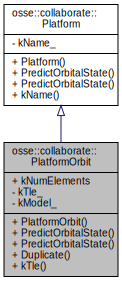
\includegraphics[width=208pt]{classosse_1_1collaborate_1_1_platform_orbit__inherit__graph}
\end{center}
\end{figure}
\subsubsection*{Public Types}
\begin{DoxyCompactItemize}
\item 
\mbox{\Hypertarget{classosse_1_1collaborate_1_1_platform_orbit_aeb5892b2982d26547cead0beebc81fe0}\label{classosse_1_1collaborate_1_1_platform_orbit_aeb5892b2982d26547cead0beebc81fe0}} 
typedef std\+::array$<$ std\+::string, \hyperlink{classosse_1_1collaborate_1_1_platform_orbit_a50b5b9308298c2a17db06a92b82abe85}{k\+Num\+Elements} $>$ \hyperlink{classosse_1_1collaborate_1_1_platform_orbit_aeb5892b2982d26547cead0beebc81fe0}{Two\+Line\+Element\+Set}
\begin{DoxyCompactList}\small\item\em A two-\/line element set. \end{DoxyCompactList}\end{DoxyCompactItemize}
\subsubsection*{Public Member Functions}
\begin{DoxyCompactItemize}
\item 
\hyperlink{classosse_1_1collaborate_1_1_platform_orbit_a7883ef54a0b5d13497fd6d21c3bd2ebf}{Platform\+Orbit} (const \hyperlink{classosse_1_1collaborate_1_1_platform_orbit_aeb5892b2982d26547cead0beebc81fe0}{Two\+Line\+Element\+Set} \&\+\_\+tle)
\begin{DoxyCompactList}\small\item\em Constructor from T\+LE. \end{DoxyCompactList}\item 
\hyperlink{classosse_1_1collaborate_1_1_orbital_state}{Orbital\+State} \hyperlink{classosse_1_1collaborate_1_1_platform_orbit_a6741aa8faec9968fd8353214d2022648}{Predict\+Orbital\+State} (const \hyperlink{classosse_1_1collaborate_1_1_simulation_clock}{Simulation\+Clock} \&\+\_\+simulation\+\_\+clock, const uint64\+\_\+t \&\+\_\+time\+\_\+s) const
\begin{DoxyCompactList}\small\item\em Get the orbital\+\_\+state of an object the current clock time. \end{DoxyCompactList}\item 
void \hyperlink{classosse_1_1collaborate_1_1_platform_orbit_a2b97a4133cb7d82d3ea62a3470f87d72}{Predict\+Orbital\+State} (const \hyperlink{classosse_1_1collaborate_1_1_simulation_clock}{Simulation\+Clock} \&\+\_\+simulation\+\_\+clock, const uint64\+\_\+t \&\+\_\+time\+\_\+s, \hyperlink{classosse_1_1collaborate_1_1_orbital_state}{Orbital\+State} $\ast$\+\_\+orbital\+\_\+state) const
\begin{DoxyCompactList}\small\item\em Update the orbital\+\_\+state of an object the current clock time. \end{DoxyCompactList}\item 
std\+::vector$<$ \hyperlink{classosse_1_1collaborate_1_1_platform_orbit}{Platform\+Orbit} $>$ \hyperlink{classosse_1_1collaborate_1_1_platform_orbit_a7c11526ed7a47023520c8fbf3605b4c4}{Duplicate} (const uint16\+\_\+t \&\+\_\+orbit\+\_\+planes, const uint16\+\_\+t \&\+\_\+groups\+\_\+per\+\_\+plane, const uint16\+\_\+t \&\+\_\+sats\+\_\+in\+\_\+train, const uint16\+\_\+t \&\+\_\+sats\+\_\+in\+\_\+tandem, const uint16\+\_\+t \&\+\_\+train\+\_\+angle, const uint16\+\_\+t \&\+\_\+tandem\+\_\+angle) const
\begin{DoxyCompactList}\small\item\em Makes a pattern of orbits based on this. \end{DoxyCompactList}\item 
const \hyperlink{classosse_1_1collaborate_1_1_platform_orbit_aeb5892b2982d26547cead0beebc81fe0}{Two\+Line\+Element\+Set} \& \hyperlink{classosse_1_1collaborate_1_1_platform_orbit_ae0b1dac3159bb4f278091b73221cad93}{k\+Tle} () const
\begin{DoxyCompactList}\small\item\em Get Array of T\+LE strings. \end{DoxyCompactList}\end{DoxyCompactItemize}
\subsubsection*{Static Public Attributes}
\begin{DoxyCompactItemize}
\item 
\mbox{\Hypertarget{classosse_1_1collaborate_1_1_platform_orbit_a50b5b9308298c2a17db06a92b82abe85}\label{classosse_1_1collaborate_1_1_platform_orbit_a50b5b9308298c2a17db06a92b82abe85}} 
static constexpr int \hyperlink{classosse_1_1collaborate_1_1_platform_orbit_a50b5b9308298c2a17db06a92b82abe85}{k\+Num\+Elements} = 3
\begin{DoxyCompactList}\small\item\em Number of strings in a two-\/line element set. \end{DoxyCompactList}\end{DoxyCompactItemize}
\subsubsection*{Private Attributes}
\begin{DoxyCompactItemize}
\item 
\mbox{\Hypertarget{classosse_1_1collaborate_1_1_platform_orbit_a997543f1020cfa000918286b774c4aa8}\label{classosse_1_1collaborate_1_1_platform_orbit_a997543f1020cfa000918286b774c4aa8}} 
const \hyperlink{classosse_1_1collaborate_1_1_platform_orbit_aeb5892b2982d26547cead0beebc81fe0}{Two\+Line\+Element\+Set} \hyperlink{classosse_1_1collaborate_1_1_platform_orbit_a997543f1020cfa000918286b774c4aa8}{k\+Tle\+\_\+}
\begin{DoxyCompactList}\small\item\em Array of T\+LE strings. \end{DoxyCompactList}\item 
\mbox{\Hypertarget{classosse_1_1collaborate_1_1_platform_orbit_a5653e1ae6b7a6274f0ecfdb423b25606}\label{classosse_1_1collaborate_1_1_platform_orbit_a5653e1ae6b7a6274f0ecfdb423b25606}} 
const sgp4\+::\+S\+G\+P4 \hyperlink{classosse_1_1collaborate_1_1_platform_orbit_a5653e1ae6b7a6274f0ecfdb423b25606}{k\+Model\+\_\+}
\begin{DoxyCompactList}\small\item\em S\+G\+P4 orbital model. \end{DoxyCompactList}\end{DoxyCompactItemize}


\subsubsection{Detailed Description}
Propogates the position of a satellite. 

 
\begin{DoxyImageNoCaption}
  \mbox{\includegraphics[width=\textwidth]{constellations}}
\end{DoxyImageNoCaption}
 

\subsubsection{Constructor \& Destructor Documentation}
\mbox{\Hypertarget{classosse_1_1collaborate_1_1_platform_orbit_a7883ef54a0b5d13497fd6d21c3bd2ebf}\label{classosse_1_1collaborate_1_1_platform_orbit_a7883ef54a0b5d13497fd6d21c3bd2ebf}} 
\index{osse\+::collaborate\+::\+Platform\+Orbit@{osse\+::collaborate\+::\+Platform\+Orbit}!Platform\+Orbit@{Platform\+Orbit}}
\index{Platform\+Orbit@{Platform\+Orbit}!osse\+::collaborate\+::\+Platform\+Orbit@{osse\+::collaborate\+::\+Platform\+Orbit}}
\paragraph{\texorpdfstring{Platform\+Orbit()}{PlatformOrbit()}}
{\footnotesize\ttfamily osse\+::collaborate\+::\+Platform\+Orbit\+::\+Platform\+Orbit (\begin{DoxyParamCaption}\item[{const \hyperlink{classosse_1_1collaborate_1_1_platform_orbit_aeb5892b2982d26547cead0beebc81fe0}{Two\+Line\+Element\+Set} \&}]{\+\_\+tle }\end{DoxyParamCaption})\hspace{0.3cm}{\ttfamily [explicit]}}



Constructor from T\+LE. 


\begin{DoxyParams}[1]{Parameters}
\mbox{\tt in}  & {\em \+\_\+tle} & Two-\/line element set \\
\hline
\end{DoxyParams}


\subsubsection{Member Function Documentation}
\mbox{\Hypertarget{classosse_1_1collaborate_1_1_platform_orbit_a7c11526ed7a47023520c8fbf3605b4c4}\label{classosse_1_1collaborate_1_1_platform_orbit_a7c11526ed7a47023520c8fbf3605b4c4}} 
\index{osse\+::collaborate\+::\+Platform\+Orbit@{osse\+::collaborate\+::\+Platform\+Orbit}!Duplicate@{Duplicate}}
\index{Duplicate@{Duplicate}!osse\+::collaborate\+::\+Platform\+Orbit@{osse\+::collaborate\+::\+Platform\+Orbit}}
\paragraph{\texorpdfstring{Duplicate()}{Duplicate()}}
{\footnotesize\ttfamily std\+::vector$<$ \hyperlink{classosse_1_1collaborate_1_1_platform_orbit}{Platform\+Orbit} $>$ osse\+::collaborate\+::\+Platform\+Orbit\+::\+Duplicate (\begin{DoxyParamCaption}\item[{const uint16\+\_\+t \&}]{\+\_\+orbit\+\_\+planes,  }\item[{const uint16\+\_\+t \&}]{\+\_\+groups\+\_\+per\+\_\+plane,  }\item[{const uint16\+\_\+t \&}]{\+\_\+sats\+\_\+in\+\_\+train,  }\item[{const uint16\+\_\+t \&}]{\+\_\+sats\+\_\+in\+\_\+tandem,  }\item[{const uint16\+\_\+t \&}]{\+\_\+train\+\_\+angle,  }\item[{const uint16\+\_\+t \&}]{\+\_\+tandem\+\_\+angle }\end{DoxyParamCaption}) const}



Makes a pattern of orbits based on this. 


\begin{DoxyParams}[1]{Parameters}
\mbox{\tt in}  & {\em \+\_\+orbit\+\_\+planes} & Number of orbit planes \\
\hline
\mbox{\tt in}  & {\em \+\_\+groups\+\_\+per\+\_\+plane} & Number of groups per plane \\
\hline
\mbox{\tt in}  & {\em \+\_\+sats\+\_\+in\+\_\+train} & Number of satellites in a train \\
\hline
\mbox{\tt in}  & {\em \+\_\+sats\+\_\+in\+\_\+tandem} & Number of satellites in tandem \\
\hline
\mbox{\tt in}  & {\em \+\_\+train\+\_\+angle} & Angle between train satellites \\
\hline
\mbox{\tt in}  & {\em \+\_\+tandem\+\_\+angle} & Angle between tandem satellites \\
\hline
\end{DoxyParams}
\begin{DoxyReturn}{Returns}
pattern\+\_\+ A list of orbits 
\end{DoxyReturn}
\mbox{\Hypertarget{classosse_1_1collaborate_1_1_platform_orbit_ae0b1dac3159bb4f278091b73221cad93}\label{classosse_1_1collaborate_1_1_platform_orbit_ae0b1dac3159bb4f278091b73221cad93}} 
\index{osse\+::collaborate\+::\+Platform\+Orbit@{osse\+::collaborate\+::\+Platform\+Orbit}!k\+Tle@{k\+Tle}}
\index{k\+Tle@{k\+Tle}!osse\+::collaborate\+::\+Platform\+Orbit@{osse\+::collaborate\+::\+Platform\+Orbit}}
\paragraph{\texorpdfstring{k\+Tle()}{kTle()}}
{\footnotesize\ttfamily const \hyperlink{classosse_1_1collaborate_1_1_platform_orbit_aeb5892b2982d26547cead0beebc81fe0}{Two\+Line\+Element\+Set}\& osse\+::collaborate\+::\+Platform\+Orbit\+::k\+Tle (\begin{DoxyParamCaption}{ }\end{DoxyParamCaption}) const\hspace{0.3cm}{\ttfamily [inline]}}



Get Array of T\+LE strings. 

\begin{DoxyReturn}{Returns}
k\+Tle\+\_\+ Array of T\+LE strings 
\end{DoxyReturn}
\mbox{\Hypertarget{classosse_1_1collaborate_1_1_platform_orbit_a6741aa8faec9968fd8353214d2022648}\label{classosse_1_1collaborate_1_1_platform_orbit_a6741aa8faec9968fd8353214d2022648}} 
\index{osse\+::collaborate\+::\+Platform\+Orbit@{osse\+::collaborate\+::\+Platform\+Orbit}!Predict\+Orbital\+State@{Predict\+Orbital\+State}}
\index{Predict\+Orbital\+State@{Predict\+Orbital\+State}!osse\+::collaborate\+::\+Platform\+Orbit@{osse\+::collaborate\+::\+Platform\+Orbit}}
\paragraph{\texorpdfstring{Predict\+Orbital\+State()}{PredictOrbitalState()}\hspace{0.1cm}{\footnotesize\ttfamily [1/2]}}
{\footnotesize\ttfamily \hyperlink{classosse_1_1collaborate_1_1_orbital_state}{Orbital\+State} osse\+::collaborate\+::\+Platform\+Orbit\+::\+Predict\+Orbital\+State (\begin{DoxyParamCaption}\item[{const \hyperlink{classosse_1_1collaborate_1_1_simulation_clock}{Simulation\+Clock} \&}]{\+\_\+simulation\+\_\+clock,  }\item[{const uint64\+\_\+t \&}]{\+\_\+time\+\_\+s }\end{DoxyParamCaption}) const\hspace{0.3cm}{\ttfamily [virtual]}}



Get the orbital\+\_\+state of an object the current clock time. 


\begin{DoxyParams}[1]{Parameters}
\mbox{\tt in}  & {\em \+\_\+simulation\+\_\+clock} & Simulation clock \\
\hline
\mbox{\tt in}  & {\em \+\_\+time\+\_\+s} & Time offset from the current time (seconds) \\
\hline
\end{DoxyParams}
\begin{DoxyReturn}{Returns}
\hyperlink{classosse_1_1collaborate_1_1_orbital_state}{Orbital\+State} of an object the current clock time 
\end{DoxyReturn}


Implements \hyperlink{classosse_1_1collaborate_1_1_platform_ad7070fcb9d91b22f25dbe0211ba0cc73}{osse\+::collaborate\+::\+Platform}.

\mbox{\Hypertarget{classosse_1_1collaborate_1_1_platform_orbit_a2b97a4133cb7d82d3ea62a3470f87d72}\label{classosse_1_1collaborate_1_1_platform_orbit_a2b97a4133cb7d82d3ea62a3470f87d72}} 
\index{osse\+::collaborate\+::\+Platform\+Orbit@{osse\+::collaborate\+::\+Platform\+Orbit}!Predict\+Orbital\+State@{Predict\+Orbital\+State}}
\index{Predict\+Orbital\+State@{Predict\+Orbital\+State}!osse\+::collaborate\+::\+Platform\+Orbit@{osse\+::collaborate\+::\+Platform\+Orbit}}
\paragraph{\texorpdfstring{Predict\+Orbital\+State()}{PredictOrbitalState()}\hspace{0.1cm}{\footnotesize\ttfamily [2/2]}}
{\footnotesize\ttfamily void osse\+::collaborate\+::\+Platform\+Orbit\+::\+Predict\+Orbital\+State (\begin{DoxyParamCaption}\item[{const \hyperlink{classosse_1_1collaborate_1_1_simulation_clock}{Simulation\+Clock} \&}]{\+\_\+simulation\+\_\+clock,  }\item[{const uint64\+\_\+t \&}]{\+\_\+time\+\_\+s,  }\item[{\hyperlink{classosse_1_1collaborate_1_1_orbital_state}{Orbital\+State} $\ast$}]{\+\_\+orbital\+\_\+state }\end{DoxyParamCaption}) const\hspace{0.3cm}{\ttfamily [virtual]}}



Update the orbital\+\_\+state of an object the current clock time. 


\begin{DoxyParams}[1]{Parameters}
\mbox{\tt in}  & {\em \+\_\+simulation\+\_\+clock} & Simulation clock \\
\hline
\mbox{\tt in}  & {\em \+\_\+time\+\_\+s} & Time offset from the current time (seconds) \\
\hline
\mbox{\tt in}  & {\em \+\_\+orbital\+\_\+state} & \hyperlink{classosse_1_1collaborate_1_1_orbital_state}{Orbital\+State} \\
\hline
\end{DoxyParams}


Implements \hyperlink{classosse_1_1collaborate_1_1_platform_a15881a343059315acdaf018e0c2470d8}{osse\+::collaborate\+::\+Platform}.



The documentation for this class was generated from the following files\+:\begin{DoxyCompactItemize}
\item 
libs/collaborate/include/collaborate/platform\+\_\+orbit.\+h\item 
libs/collaborate/src/platform\+\_\+orbit.\+cpp\end{DoxyCompactItemize}

\hypertarget{classosse_1_1collaborate_1_1_platform}{}\subsection{osse\+:\+:collaborate\+:\+:Platform Class Reference}
\label{classosse_1_1collaborate_1_1_platform}\index{osse\+::collaborate\+::\+Platform@{osse\+::collaborate\+::\+Platform}}


Propogates a node\textquotesingle{}s position.  




{\ttfamily \#include $<$platform.\+h$>$}



Inheritance diagram for osse\+:\+:collaborate\+:\+:Platform\+:
\nopagebreak
\begin{figure}[H]
\begin{center}
\leavevmode
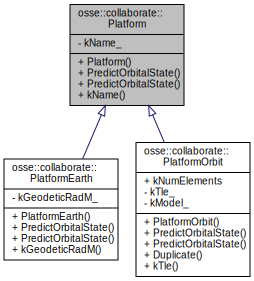
\includegraphics[width=350pt]{classosse_1_1collaborate_1_1_platform__inherit__graph}
\end{center}
\end{figure}
\subsubsection*{Public Member Functions}
\begin{DoxyCompactItemize}
\item 
\hyperlink{classosse_1_1collaborate_1_1_platform_aca95bfbb4f84285f1767d575a3e4c2ec}{Platform} (const std\+::string \&\+\_\+name)
\begin{DoxyCompactList}\small\item\em Constructor. \end{DoxyCompactList}\item 
virtual \hyperlink{classosse_1_1collaborate_1_1_orbital_state}{Orbital\+State} \hyperlink{classosse_1_1collaborate_1_1_platform_ad7070fcb9d91b22f25dbe0211ba0cc73}{Predict\+Orbital\+State} (const \hyperlink{classosse_1_1collaborate_1_1_simulation_clock}{Simulation\+Clock} \&\+\_\+clock, const uint64\+\_\+t \&\+\_\+time\+\_\+s) const =0
\begin{DoxyCompactList}\small\item\em Get the orbital\+\_\+state of an object the current clock time. \end{DoxyCompactList}\item 
virtual void \hyperlink{classosse_1_1collaborate_1_1_platform_a15881a343059315acdaf018e0c2470d8}{Predict\+Orbital\+State} (const \hyperlink{classosse_1_1collaborate_1_1_simulation_clock}{Simulation\+Clock} \&\+\_\+clock, const uint64\+\_\+t \&\+\_\+time\+\_\+s, \hyperlink{classosse_1_1collaborate_1_1_orbital_state}{Orbital\+State} $\ast$\+\_\+orbital\+\_\+state) const =0
\begin{DoxyCompactList}\small\item\em Update the orbital\+\_\+state of an object the current clock time. \end{DoxyCompactList}\item 
std\+::string \hyperlink{classosse_1_1collaborate_1_1_platform_a87b0b2589a6246dfd90ba3168ebf285c}{k\+Name} () const
\begin{DoxyCompactList}\small\item\em Gets k\+Name. \end{DoxyCompactList}\end{DoxyCompactItemize}
\subsubsection*{Private Attributes}
\begin{DoxyCompactItemize}
\item 
\mbox{\Hypertarget{classosse_1_1collaborate_1_1_platform_a00a6267a955519320627877310f90b97}\label{classosse_1_1collaborate_1_1_platform_a00a6267a955519320627877310f90b97}} 
const std\+::string \hyperlink{classosse_1_1collaborate_1_1_platform_a00a6267a955519320627877310f90b97}{k\+Name\+\_\+}
\begin{DoxyCompactList}\small\item\em Name of the platform. \end{DoxyCompactList}\end{DoxyCompactItemize}


\subsubsection{Detailed Description}
Propogates a node\textquotesingle{}s position. 

\subsubsection{Constructor \& Destructor Documentation}
\mbox{\Hypertarget{classosse_1_1collaborate_1_1_platform_aca95bfbb4f84285f1767d575a3e4c2ec}\label{classosse_1_1collaborate_1_1_platform_aca95bfbb4f84285f1767d575a3e4c2ec}} 
\index{osse\+::collaborate\+::\+Platform@{osse\+::collaborate\+::\+Platform}!Platform@{Platform}}
\index{Platform@{Platform}!osse\+::collaborate\+::\+Platform@{osse\+::collaborate\+::\+Platform}}
\paragraph{\texorpdfstring{Platform()}{Platform()}}
{\footnotesize\ttfamily osse\+::collaborate\+::\+Platform\+::\+Platform (\begin{DoxyParamCaption}\item[{const std\+::string \&}]{\+\_\+name }\end{DoxyParamCaption})\hspace{0.3cm}{\ttfamily [explicit]}}



Constructor. 


\begin{DoxyParams}[1]{Parameters}
\mbox{\tt in}  & {\em \+\_\+name} & The name of the platform \\
\hline
\end{DoxyParams}


\subsubsection{Member Function Documentation}
\mbox{\Hypertarget{classosse_1_1collaborate_1_1_platform_a87b0b2589a6246dfd90ba3168ebf285c}\label{classosse_1_1collaborate_1_1_platform_a87b0b2589a6246dfd90ba3168ebf285c}} 
\index{osse\+::collaborate\+::\+Platform@{osse\+::collaborate\+::\+Platform}!k\+Name@{k\+Name}}
\index{k\+Name@{k\+Name}!osse\+::collaborate\+::\+Platform@{osse\+::collaborate\+::\+Platform}}
\paragraph{\texorpdfstring{k\+Name()}{kName()}}
{\footnotesize\ttfamily std\+::string osse\+::collaborate\+::\+Platform\+::k\+Name (\begin{DoxyParamCaption}{ }\end{DoxyParamCaption}) const\hspace{0.3cm}{\ttfamily [inline]}}



Gets k\+Name. 

\begin{DoxyReturn}{Returns}
k\+Name\+\_\+ Name of the platform 
\end{DoxyReturn}
\mbox{\Hypertarget{classosse_1_1collaborate_1_1_platform_ad7070fcb9d91b22f25dbe0211ba0cc73}\label{classosse_1_1collaborate_1_1_platform_ad7070fcb9d91b22f25dbe0211ba0cc73}} 
\index{osse\+::collaborate\+::\+Platform@{osse\+::collaborate\+::\+Platform}!Predict\+Orbital\+State@{Predict\+Orbital\+State}}
\index{Predict\+Orbital\+State@{Predict\+Orbital\+State}!osse\+::collaborate\+::\+Platform@{osse\+::collaborate\+::\+Platform}}
\paragraph{\texorpdfstring{Predict\+Orbital\+State()}{PredictOrbitalState()}\hspace{0.1cm}{\footnotesize\ttfamily [1/2]}}
{\footnotesize\ttfamily virtual \hyperlink{classosse_1_1collaborate_1_1_orbital_state}{Orbital\+State} osse\+::collaborate\+::\+Platform\+::\+Predict\+Orbital\+State (\begin{DoxyParamCaption}\item[{const \hyperlink{classosse_1_1collaborate_1_1_simulation_clock}{Simulation\+Clock} \&}]{\+\_\+clock,  }\item[{const uint64\+\_\+t \&}]{\+\_\+time\+\_\+s }\end{DoxyParamCaption}) const\hspace{0.3cm}{\ttfamily [pure virtual]}}



Get the orbital\+\_\+state of an object the current clock time. 


\begin{DoxyParams}[1]{Parameters}
\mbox{\tt in}  & {\em \+\_\+clock} & Simulation clock \\
\hline
\mbox{\tt in}  & {\em \+\_\+time\+\_\+s} & Time offset from the current time (seconds) \\
\hline
\end{DoxyParams}
\begin{DoxyReturn}{Returns}
\hyperlink{classosse_1_1collaborate_1_1_orbital_state}{Orbital\+State} of an object at the current clock time 
\end{DoxyReturn}


Implemented in \hyperlink{classosse_1_1collaborate_1_1_platform_orbit_a6741aa8faec9968fd8353214d2022648}{osse\+::collaborate\+::\+Platform\+Orbit}, and \hyperlink{classosse_1_1collaborate_1_1_platform_earth_aff04ed83ab0ae2f7b3bcb1019588efcd}{osse\+::collaborate\+::\+Platform\+Earth}.

\mbox{\Hypertarget{classosse_1_1collaborate_1_1_platform_a15881a343059315acdaf018e0c2470d8}\label{classosse_1_1collaborate_1_1_platform_a15881a343059315acdaf018e0c2470d8}} 
\index{osse\+::collaborate\+::\+Platform@{osse\+::collaborate\+::\+Platform}!Predict\+Orbital\+State@{Predict\+Orbital\+State}}
\index{Predict\+Orbital\+State@{Predict\+Orbital\+State}!osse\+::collaborate\+::\+Platform@{osse\+::collaborate\+::\+Platform}}
\paragraph{\texorpdfstring{Predict\+Orbital\+State()}{PredictOrbitalState()}\hspace{0.1cm}{\footnotesize\ttfamily [2/2]}}
{\footnotesize\ttfamily virtual void osse\+::collaborate\+::\+Platform\+::\+Predict\+Orbital\+State (\begin{DoxyParamCaption}\item[{const \hyperlink{classosse_1_1collaborate_1_1_simulation_clock}{Simulation\+Clock} \&}]{\+\_\+clock,  }\item[{const uint64\+\_\+t \&}]{\+\_\+time\+\_\+s,  }\item[{\hyperlink{classosse_1_1collaborate_1_1_orbital_state}{Orbital\+State} $\ast$}]{\+\_\+orbital\+\_\+state }\end{DoxyParamCaption}) const\hspace{0.3cm}{\ttfamily [pure virtual]}}



Update the orbital\+\_\+state of an object the current clock time. 


\begin{DoxyParams}[1]{Parameters}
\mbox{\tt in}  & {\em \+\_\+clock} & Simulation clock \\
\hline
\mbox{\tt in}  & {\em \+\_\+time\+\_\+s} & Time offset from the current time (seconds) \\
\hline
\mbox{\tt in}  & {\em \+\_\+orbital\+\_\+state} & \hyperlink{classosse_1_1collaborate_1_1_orbital_state}{Orbital\+State} of an object \\
\hline
\end{DoxyParams}


Implemented in \hyperlink{classosse_1_1collaborate_1_1_platform_orbit_a2b97a4133cb7d82d3ea62a3470f87d72}{osse\+::collaborate\+::\+Platform\+Orbit}, and \hyperlink{classosse_1_1collaborate_1_1_platform_earth_ab49f25fe5d37334918483cfdcef3471a}{osse\+::collaborate\+::\+Platform\+Earth}.



The documentation for this class was generated from the following files\+:\begin{DoxyCompactItemize}
\item 
libs/collaborate/include/collaborate/platform.\+h\item 
libs/collaborate/src/platform.\+cpp\end{DoxyCompactItemize}

\hypertarget{classosse_1_1collaborate_1_1_reference_frame}{}\subsection{osse\+:\+:collaborate\+:\+:Reference\+Frame Class Reference}
\label{classosse_1_1collaborate_1_1_reference_frame}\index{osse\+::collaborate\+::\+Reference\+Frame@{osse\+::collaborate\+::\+Reference\+Frame}}


An attitude reference frame.  




{\ttfamily \#include $<$reference\+\_\+frame.\+h$>$}

\subsubsection*{Public Member Functions}
\begin{DoxyCompactItemize}
\item 
\hyperlink{classosse_1_1collaborate_1_1_reference_frame_aa7a87b7392e85b87cf0994457f0b5b6a}{Reference\+Frame} (const \hyperlink{classosse_1_1collaborate_1_1_vector}{Vector} \&\+\_\+x\+\_\+axis, const \hyperlink{classosse_1_1collaborate_1_1_vector}{Vector} \&\+\_\+y\+\_\+axis, const \hyperlink{classosse_1_1collaborate_1_1_vector}{Vector} \&\+\_\+z\+\_\+axis)
\begin{DoxyCompactList}\small\item\em Constructor from axes. \end{DoxyCompactList}\item 
\hyperlink{classosse_1_1collaborate_1_1_reference_frame_ab6e3506c308d48e033730fa71c3721af}{Reference\+Frame} (const double \&\+\_\+roll\+\_\+rad, const double \&\+\_\+pitch\+\_\+rad, const double \&\+\_\+yaw\+\_\+rad)
\begin{DoxyCompactList}\small\item\em Constructor from angles. \end{DoxyCompactList}\item 
\hyperlink{classosse_1_1collaborate_1_1_reference_frame_a09500c8f97064fa3d907913e26f2df90}{Reference\+Frame} (const \hyperlink{classosse_1_1collaborate_1_1_reference_frame}{Reference\+Frame} \&\+\_\+frame, const double \&\+\_\+roll\+\_\+rad, const double \&\+\_\+pitch\+\_\+rad, const double \&\+\_\+yaw\+\_\+rad)
\begin{DoxyCompactList}\small\item\em Constructor from reference frame and rotation angles. \end{DoxyCompactList}\item 
\hyperlink{classosse_1_1collaborate_1_1_reference_frame_a603c3443d0d09086de9e95cd69b62ea5}{Reference\+Frame} (const \hyperlink{classosse_1_1collaborate_1_1_reference_frame}{Reference\+Frame} \&\+\_\+frame\+\_\+1, const \hyperlink{classosse_1_1collaborate_1_1_reference_frame}{Reference\+Frame} \&\+\_\+frame\+\_\+2, const double \&\+\_\+roll\+\_\+rad, const double \&\+\_\+pitch\+\_\+rad, const double \&\+\_\+yaw\+\_\+rad)
\begin{DoxyCompactList}\small\item\em Constructor from two reference frames and rotation angles. \end{DoxyCompactList}\item 
void \hyperlink{classosse_1_1collaborate_1_1_reference_frame_a0d731be5e188825229a59440eea5341e}{Update} (const \hyperlink{classosse_1_1collaborate_1_1_reference_frame}{Reference\+Frame} \&\+\_\+frame)
\begin{DoxyCompactList}\small\item\em Updates axes relative to a single reference frame. \end{DoxyCompactList}\item 
void \hyperlink{classosse_1_1collaborate_1_1_reference_frame_aa32123d1bb0af3ba1f3bb68d72c8e6e3}{Update} (const \hyperlink{classosse_1_1collaborate_1_1_reference_frame}{Reference\+Frame} \&\+\_\+frame\+\_\+1, const \hyperlink{classosse_1_1collaborate_1_1_reference_frame}{Reference\+Frame} \&\+\_\+frame\+\_\+2)
\begin{DoxyCompactList}\small\item\em Updates axes relative to a single reference frame. \end{DoxyCompactList}\item 
std\+::vector$<$ double $>$ \hyperlink{classosse_1_1collaborate_1_1_reference_frame_ac448c98f8206e372f7c367b511f008e6}{Obtain\+Log} () const
\begin{DoxyCompactList}\small\item\em Logs the \hyperlink{classosse_1_1collaborate_1_1_reference_frame}{Reference\+Frame}. \end{DoxyCompactList}\item 
void \hyperlink{classosse_1_1collaborate_1_1_reference_frame_adf108795332e39e7975d7bfe69774b78}{set\+\_\+z\+\_\+axis} (const \hyperlink{classosse_1_1collaborate_1_1_vector}{Vector} \&\+\_\+z\+\_\+axis)
\begin{DoxyCompactList}\small\item\em Set z-\/axis. \end{DoxyCompactList}\item 
void \hyperlink{classosse_1_1collaborate_1_1_reference_frame_a239519dbae2c753b8763d5b39d97e93d}{set\+\_\+y\+\_\+axis} (const \hyperlink{classosse_1_1collaborate_1_1_vector}{Vector} \&\+\_\+y\+\_\+axis)
\begin{DoxyCompactList}\small\item\em Set y-\/axis. \end{DoxyCompactList}\item 
void \hyperlink{classosse_1_1collaborate_1_1_reference_frame_a58806d59231dd107bf2b25a0a7396266}{set\+\_\+x\+\_\+axis} (const \hyperlink{classosse_1_1collaborate_1_1_vector}{Vector} \&\+\_\+x\+\_\+axis)
\begin{DoxyCompactList}\small\item\em Set x-\/axis. \end{DoxyCompactList}\item 
const \hyperlink{classosse_1_1collaborate_1_1_attitude_matrix}{Attitude\+Matrix} \& \hyperlink{classosse_1_1collaborate_1_1_reference_frame_a518335e6d01a2b8c50f00402818d22b9}{attitude} () const
\begin{DoxyCompactList}\small\item\em Get attitude attitude\+\_\+matrix. \end{DoxyCompactList}\item 
const \hyperlink{classosse_1_1collaborate_1_1_vector}{Vector} \& \hyperlink{classosse_1_1collaborate_1_1_reference_frame_ad3fcddd11a85e828e7de51b333bdf12b}{z\+\_\+axis} () const
\begin{DoxyCompactList}\small\item\em Get z-\/axis. \end{DoxyCompactList}\item 
const \hyperlink{classosse_1_1collaborate_1_1_vector}{Vector} \& \hyperlink{classosse_1_1collaborate_1_1_reference_frame_ae37a2e46a6ed1868a12829e461e6e423}{y\+\_\+axis} () const
\begin{DoxyCompactList}\small\item\em Get y-\/axis. \end{DoxyCompactList}\item 
const \hyperlink{classosse_1_1collaborate_1_1_vector}{Vector} \& \hyperlink{classosse_1_1collaborate_1_1_reference_frame_ac2b2705500ac17535e5ec8127684b449}{x\+\_\+axis} () const
\begin{DoxyCompactList}\small\item\em Get x-\/axis. \end{DoxyCompactList}\item 
std\+::string \hyperlink{classosse_1_1collaborate_1_1_reference_frame_ae5b5e9f9dcb5841fbeb910402afc3b77}{To\+String} () const
\begin{DoxyCompactList}\small\item\em Outputs \hyperlink{classosse_1_1collaborate_1_1_reference_frame}{Reference\+Frame} to a string. \end{DoxyCompactList}\end{DoxyCompactItemize}
\subsubsection*{Private Member Functions}
\begin{DoxyCompactItemize}
\item 
\hyperlink{classosse_1_1collaborate_1_1_vector}{Vector} \hyperlink{classosse_1_1collaborate_1_1_reference_frame_a560f99ed2e6d7298cffbfbab84fe4a94}{Transform\+X\+Axis} (const \hyperlink{classosse_1_1collaborate_1_1_reference_frame}{Reference\+Frame} \&\+\_\+frame) const
\begin{DoxyCompactList}\small\item\em Transforms Earth\textquotesingle{}s x-\/axis through single reference. \end{DoxyCompactList}\item 
\hyperlink{classosse_1_1collaborate_1_1_vector}{Vector} \hyperlink{classosse_1_1collaborate_1_1_reference_frame_a417ac4bad191e12f1aaff76e413f339e}{Transform\+Y\+Axis} (const \hyperlink{classosse_1_1collaborate_1_1_reference_frame}{Reference\+Frame} \&\+\_\+frame) const
\begin{DoxyCompactList}\small\item\em Transforms Earth\textquotesingle{}s y-\/axis through single reference. \end{DoxyCompactList}\item 
\hyperlink{classosse_1_1collaborate_1_1_vector}{Vector} \hyperlink{classosse_1_1collaborate_1_1_reference_frame_a7fc4ac945236cd63ed4c3bddd5149594}{Transform\+Z\+Axis} (const \hyperlink{classosse_1_1collaborate_1_1_reference_frame}{Reference\+Frame} \&\+\_\+frame) const
\begin{DoxyCompactList}\small\item\em Transforms Earth\textquotesingle{}s z-\/axis through single reference. \end{DoxyCompactList}\item 
\hyperlink{classosse_1_1collaborate_1_1_vector}{Vector} \hyperlink{classosse_1_1collaborate_1_1_reference_frame_a2172488c952b75bca793b4eca308b50b}{Transform\+X\+Axis} (const \hyperlink{classosse_1_1collaborate_1_1_reference_frame}{Reference\+Frame} \&\+\_\+frame\+\_\+1, const \hyperlink{classosse_1_1collaborate_1_1_reference_frame}{Reference\+Frame} \&\+\_\+frame\+\_\+2) const
\begin{DoxyCompactList}\small\item\em Transforms Earth\textquotesingle{}s x-\/axis through two reference frames. \end{DoxyCompactList}\item 
\hyperlink{classosse_1_1collaborate_1_1_vector}{Vector} \hyperlink{classosse_1_1collaborate_1_1_reference_frame_a7f321d33340f957142db898ce6d91b7a}{Transform\+Y\+Axis} (const \hyperlink{classosse_1_1collaborate_1_1_reference_frame}{Reference\+Frame} \&\+\_\+frame\+\_\+1, const \hyperlink{classosse_1_1collaborate_1_1_reference_frame}{Reference\+Frame} \&\+\_\+frame\+\_\+2) const
\begin{DoxyCompactList}\small\item\em Transforms Earth\textquotesingle{}s y-\/axis through two reference frames. \end{DoxyCompactList}\item 
\hyperlink{classosse_1_1collaborate_1_1_vector}{Vector} \hyperlink{classosse_1_1collaborate_1_1_reference_frame_a2b99f8d49fc9c61b8dc98118469aeb38}{Transform\+Z\+Axis} (const \hyperlink{classosse_1_1collaborate_1_1_reference_frame}{Reference\+Frame} \&\+\_\+frame\+\_\+1, const \hyperlink{classosse_1_1collaborate_1_1_reference_frame}{Reference\+Frame} \&\+\_\+frame\+\_\+2) const
\begin{DoxyCompactList}\small\item\em Transforms Earth\textquotesingle{}s z-\/axis through two reference frames. \end{DoxyCompactList}\end{DoxyCompactItemize}
\subsubsection*{Private Attributes}
\begin{DoxyCompactItemize}
\item 
\mbox{\Hypertarget{classosse_1_1collaborate_1_1_reference_frame_a090dbed30d878898de54dde3396c9834}\label{classosse_1_1collaborate_1_1_reference_frame_a090dbed30d878898de54dde3396c9834}} 
\hyperlink{classosse_1_1collaborate_1_1_attitude_matrix}{Attitude\+Matrix} \hyperlink{classosse_1_1collaborate_1_1_reference_frame_a090dbed30d878898de54dde3396c9834}{attitude\+\_\+}
\begin{DoxyCompactList}\small\item\em Attitude attitude\+\_\+matrix. \end{DoxyCompactList}\item 
\mbox{\Hypertarget{classosse_1_1collaborate_1_1_reference_frame_a75537f26c0568f35ee4c42def52efa55}\label{classosse_1_1collaborate_1_1_reference_frame_a75537f26c0568f35ee4c42def52efa55}} 
\hyperlink{classosse_1_1collaborate_1_1_vector}{Vector} \hyperlink{classosse_1_1collaborate_1_1_reference_frame_a75537f26c0568f35ee4c42def52efa55}{x\+\_\+axis\+\_\+}
\begin{DoxyCompactList}\small\item\em X-\/axis. \end{DoxyCompactList}\item 
\mbox{\Hypertarget{classosse_1_1collaborate_1_1_reference_frame_a332173d954b5201f1ab5a07be1154c87}\label{classosse_1_1collaborate_1_1_reference_frame_a332173d954b5201f1ab5a07be1154c87}} 
\hyperlink{classosse_1_1collaborate_1_1_vector}{Vector} \hyperlink{classosse_1_1collaborate_1_1_reference_frame_a332173d954b5201f1ab5a07be1154c87}{y\+\_\+axis\+\_\+}
\begin{DoxyCompactList}\small\item\em Y-\/axis. \end{DoxyCompactList}\item 
\mbox{\Hypertarget{classosse_1_1collaborate_1_1_reference_frame_acd8265229993f949f611129283ec7645}\label{classosse_1_1collaborate_1_1_reference_frame_acd8265229993f949f611129283ec7645}} 
\hyperlink{classosse_1_1collaborate_1_1_vector}{Vector} \hyperlink{classosse_1_1collaborate_1_1_reference_frame_acd8265229993f949f611129283ec7645}{z\+\_\+axis\+\_\+}
\begin{DoxyCompactList}\small\item\em Z-\/axis. \end{DoxyCompactList}\end{DoxyCompactItemize}


\subsubsection{Detailed Description}
An attitude reference frame. 

 
\begin{DoxyImageNoCaption}
  \mbox{\includegraphics[width=0.5\textwidth]{frames}}
\end{DoxyImageNoCaption}


\[ \vec{x}_{axis}, \vec{y}_{axis}, \vec{z}_{axis} = \begin{bmatrix} x_x\\x_y\\x_z \end{bmatrix},~ \begin{bmatrix} y_x\\y_y\\y_z \end{bmatrix},~ \begin{bmatrix} z_x\\z_y\\z_z \end{bmatrix} ~~~(unit~vectors) \] \[ {\bf{A}} = Attitude~AttitudeMatrix = \begin{bmatrix} a_{0,0} & a_{0,1} & a_{0,2} \\ a_{1,0} & a_{1,1} & a_{1,2} \\ a_{2,0} & a_{2,1} & a_{2,2} \end{bmatrix} \] 

\subsubsection{Constructor \& Destructor Documentation}
\mbox{\Hypertarget{classosse_1_1collaborate_1_1_reference_frame_aa7a87b7392e85b87cf0994457f0b5b6a}\label{classosse_1_1collaborate_1_1_reference_frame_aa7a87b7392e85b87cf0994457f0b5b6a}} 
\index{osse\+::collaborate\+::\+Reference\+Frame@{osse\+::collaborate\+::\+Reference\+Frame}!Reference\+Frame@{Reference\+Frame}}
\index{Reference\+Frame@{Reference\+Frame}!osse\+::collaborate\+::\+Reference\+Frame@{osse\+::collaborate\+::\+Reference\+Frame}}
\paragraph{\texorpdfstring{Reference\+Frame()}{ReferenceFrame()}\hspace{0.1cm}{\footnotesize\ttfamily [1/4]}}
{\footnotesize\ttfamily osse\+::collaborate\+::\+Reference\+Frame\+::\+Reference\+Frame (\begin{DoxyParamCaption}\item[{const \hyperlink{classosse_1_1collaborate_1_1_vector}{Vector} \&}]{\+\_\+x\+\_\+axis,  }\item[{const \hyperlink{classosse_1_1collaborate_1_1_vector}{Vector} \&}]{\+\_\+y\+\_\+axis,  }\item[{const \hyperlink{classosse_1_1collaborate_1_1_vector}{Vector} \&}]{\+\_\+z\+\_\+axis }\end{DoxyParamCaption})}



Constructor from axes. 


\begin{DoxyParams}[1]{Parameters}
\mbox{\tt in}  & {\em \+\_\+x\+\_\+axis} & X-\/axis (unit) \\
\hline
\mbox{\tt in}  & {\em \+\_\+y\+\_\+axis} & Y-\/axis (unit) \\
\hline
\mbox{\tt in}  & {\em \+\_\+z\+\_\+axis} & Z-\/axis (unit) \\
\hline
\end{DoxyParams}
\mbox{\Hypertarget{classosse_1_1collaborate_1_1_reference_frame_ab6e3506c308d48e033730fa71c3721af}\label{classosse_1_1collaborate_1_1_reference_frame_ab6e3506c308d48e033730fa71c3721af}} 
\index{osse\+::collaborate\+::\+Reference\+Frame@{osse\+::collaborate\+::\+Reference\+Frame}!Reference\+Frame@{Reference\+Frame}}
\index{Reference\+Frame@{Reference\+Frame}!osse\+::collaborate\+::\+Reference\+Frame@{osse\+::collaborate\+::\+Reference\+Frame}}
\paragraph{\texorpdfstring{Reference\+Frame()}{ReferenceFrame()}\hspace{0.1cm}{\footnotesize\ttfamily [2/4]}}
{\footnotesize\ttfamily osse\+::collaborate\+::\+Reference\+Frame\+::\+Reference\+Frame (\begin{DoxyParamCaption}\item[{const double \&}]{\+\_\+roll\+\_\+rad,  }\item[{const double \&}]{\+\_\+pitch\+\_\+rad,  }\item[{const double \&}]{\+\_\+yaw\+\_\+rad }\end{DoxyParamCaption})}



Constructor from angles. 


\begin{DoxyParams}[1]{Parameters}
\mbox{\tt in}  & {\em \+\_\+roll\+\_\+rad} & Rotation about the x-\/axis \\
\hline
\mbox{\tt in}  & {\em \+\_\+pitch\+\_\+rad} & Rotation about the y-\/axis \\
\hline
\mbox{\tt in}  & {\em \+\_\+yaw\+\_\+rad} & Rotation about the z-\/axis \\
\hline
\end{DoxyParams}
\mbox{\Hypertarget{classosse_1_1collaborate_1_1_reference_frame_a09500c8f97064fa3d907913e26f2df90}\label{classosse_1_1collaborate_1_1_reference_frame_a09500c8f97064fa3d907913e26f2df90}} 
\index{osse\+::collaborate\+::\+Reference\+Frame@{osse\+::collaborate\+::\+Reference\+Frame}!Reference\+Frame@{Reference\+Frame}}
\index{Reference\+Frame@{Reference\+Frame}!osse\+::collaborate\+::\+Reference\+Frame@{osse\+::collaborate\+::\+Reference\+Frame}}
\paragraph{\texorpdfstring{Reference\+Frame()}{ReferenceFrame()}\hspace{0.1cm}{\footnotesize\ttfamily [3/4]}}
{\footnotesize\ttfamily osse\+::collaborate\+::\+Reference\+Frame\+::\+Reference\+Frame (\begin{DoxyParamCaption}\item[{const \hyperlink{classosse_1_1collaborate_1_1_reference_frame}{Reference\+Frame} \&}]{\+\_\+frame,  }\item[{const double \&}]{\+\_\+roll\+\_\+rad,  }\item[{const double \&}]{\+\_\+pitch\+\_\+rad,  }\item[{const double \&}]{\+\_\+yaw\+\_\+rad }\end{DoxyParamCaption})}



Constructor from reference frame and rotation angles. 


\begin{DoxyParams}[1]{Parameters}
\mbox{\tt in}  & {\em \+\_\+frame} & Reference frame \\
\hline
\mbox{\tt in}  & {\em \+\_\+roll\+\_\+rad} & Rotation about the x-\/axis \\
\hline
\mbox{\tt in}  & {\em \+\_\+pitch\+\_\+rad} & Rotation about the y-\/axis \\
\hline
\mbox{\tt in}  & {\em \+\_\+yaw\+\_\+rad} & Rotation about the z-\/axis \\
\hline
\end{DoxyParams}
\mbox{\Hypertarget{classosse_1_1collaborate_1_1_reference_frame_a603c3443d0d09086de9e95cd69b62ea5}\label{classosse_1_1collaborate_1_1_reference_frame_a603c3443d0d09086de9e95cd69b62ea5}} 
\index{osse\+::collaborate\+::\+Reference\+Frame@{osse\+::collaborate\+::\+Reference\+Frame}!Reference\+Frame@{Reference\+Frame}}
\index{Reference\+Frame@{Reference\+Frame}!osse\+::collaborate\+::\+Reference\+Frame@{osse\+::collaborate\+::\+Reference\+Frame}}
\paragraph{\texorpdfstring{Reference\+Frame()}{ReferenceFrame()}\hspace{0.1cm}{\footnotesize\ttfamily [4/4]}}
{\footnotesize\ttfamily osse\+::collaborate\+::\+Reference\+Frame\+::\+Reference\+Frame (\begin{DoxyParamCaption}\item[{const \hyperlink{classosse_1_1collaborate_1_1_reference_frame}{Reference\+Frame} \&}]{\+\_\+frame\+\_\+1,  }\item[{const \hyperlink{classosse_1_1collaborate_1_1_reference_frame}{Reference\+Frame} \&}]{\+\_\+frame\+\_\+2,  }\item[{const double \&}]{\+\_\+roll\+\_\+rad,  }\item[{const double \&}]{\+\_\+pitch\+\_\+rad,  }\item[{const double \&}]{\+\_\+yaw\+\_\+rad }\end{DoxyParamCaption})}



Constructor from two reference frames and rotation angles. 


\begin{DoxyParams}[1]{Parameters}
\mbox{\tt in}  & {\em \+\_\+frame\+\_\+1} & First reference frame \\
\hline
\mbox{\tt in}  & {\em \+\_\+frame\+\_\+2} & Second reference frame \\
\hline
\mbox{\tt in}  & {\em \+\_\+roll\+\_\+rad} & Rotation about the x-\/axis \\
\hline
\mbox{\tt in}  & {\em \+\_\+pitch\+\_\+rad} & Rotation about the y-\/axis \\
\hline
\mbox{\tt in}  & {\em \+\_\+yaw\+\_\+rad} & Rotation about the z-\/axis \\
\hline
\end{DoxyParams}


\subsubsection{Member Function Documentation}
\mbox{\Hypertarget{classosse_1_1collaborate_1_1_reference_frame_a518335e6d01a2b8c50f00402818d22b9}\label{classosse_1_1collaborate_1_1_reference_frame_a518335e6d01a2b8c50f00402818d22b9}} 
\index{osse\+::collaborate\+::\+Reference\+Frame@{osse\+::collaborate\+::\+Reference\+Frame}!attitude@{attitude}}
\index{attitude@{attitude}!osse\+::collaborate\+::\+Reference\+Frame@{osse\+::collaborate\+::\+Reference\+Frame}}
\paragraph{\texorpdfstring{attitude()}{attitude()}}
{\footnotesize\ttfamily const \hyperlink{classosse_1_1collaborate_1_1_attitude_matrix}{Attitude\+Matrix}\& osse\+::collaborate\+::\+Reference\+Frame\+::attitude (\begin{DoxyParamCaption}{ }\end{DoxyParamCaption}) const\hspace{0.3cm}{\ttfamily [inline]}}



Get attitude attitude\+\_\+matrix. 

\begin{DoxyReturn}{Returns}
attitude\+\_\+ Attitude attitude\+\_\+matrix 
\end{DoxyReturn}
\mbox{\Hypertarget{classosse_1_1collaborate_1_1_reference_frame_ac448c98f8206e372f7c367b511f008e6}\label{classosse_1_1collaborate_1_1_reference_frame_ac448c98f8206e372f7c367b511f008e6}} 
\index{osse\+::collaborate\+::\+Reference\+Frame@{osse\+::collaborate\+::\+Reference\+Frame}!Obtain\+Log@{Obtain\+Log}}
\index{Obtain\+Log@{Obtain\+Log}!osse\+::collaborate\+::\+Reference\+Frame@{osse\+::collaborate\+::\+Reference\+Frame}}
\paragraph{\texorpdfstring{Obtain\+Log()}{ObtainLog()}}
{\footnotesize\ttfamily std\+::vector$<$ double $>$ osse\+::collaborate\+::\+Reference\+Frame\+::\+Obtain\+Log (\begin{DoxyParamCaption}{ }\end{DoxyParamCaption}) const}



Logs the \hyperlink{classosse_1_1collaborate_1_1_reference_frame}{Reference\+Frame}. 

\begin{DoxyReturn}{Returns}
A vector of doubles 
\end{DoxyReturn}
\mbox{\Hypertarget{classosse_1_1collaborate_1_1_reference_frame_a58806d59231dd107bf2b25a0a7396266}\label{classosse_1_1collaborate_1_1_reference_frame_a58806d59231dd107bf2b25a0a7396266}} 
\index{osse\+::collaborate\+::\+Reference\+Frame@{osse\+::collaborate\+::\+Reference\+Frame}!set\+\_\+x\+\_\+axis@{set\+\_\+x\+\_\+axis}}
\index{set\+\_\+x\+\_\+axis@{set\+\_\+x\+\_\+axis}!osse\+::collaborate\+::\+Reference\+Frame@{osse\+::collaborate\+::\+Reference\+Frame}}
\paragraph{\texorpdfstring{set\+\_\+x\+\_\+axis()}{set\_x\_axis()}}
{\footnotesize\ttfamily void osse\+::collaborate\+::\+Reference\+Frame\+::set\+\_\+x\+\_\+axis (\begin{DoxyParamCaption}\item[{const \hyperlink{classosse_1_1collaborate_1_1_vector}{Vector} \&}]{\+\_\+x\+\_\+axis }\end{DoxyParamCaption})\hspace{0.3cm}{\ttfamily [inline]}}



Set x-\/axis. 


\begin{DoxyParams}[1]{Parameters}
\mbox{\tt in}  & {\em \+\_\+x\+\_\+axis} & X-\/axis \\
\hline
\end{DoxyParams}
\mbox{\Hypertarget{classosse_1_1collaborate_1_1_reference_frame_a239519dbae2c753b8763d5b39d97e93d}\label{classosse_1_1collaborate_1_1_reference_frame_a239519dbae2c753b8763d5b39d97e93d}} 
\index{osse\+::collaborate\+::\+Reference\+Frame@{osse\+::collaborate\+::\+Reference\+Frame}!set\+\_\+y\+\_\+axis@{set\+\_\+y\+\_\+axis}}
\index{set\+\_\+y\+\_\+axis@{set\+\_\+y\+\_\+axis}!osse\+::collaborate\+::\+Reference\+Frame@{osse\+::collaborate\+::\+Reference\+Frame}}
\paragraph{\texorpdfstring{set\+\_\+y\+\_\+axis()}{set\_y\_axis()}}
{\footnotesize\ttfamily void osse\+::collaborate\+::\+Reference\+Frame\+::set\+\_\+y\+\_\+axis (\begin{DoxyParamCaption}\item[{const \hyperlink{classosse_1_1collaborate_1_1_vector}{Vector} \&}]{\+\_\+y\+\_\+axis }\end{DoxyParamCaption})\hspace{0.3cm}{\ttfamily [inline]}}



Set y-\/axis. 


\begin{DoxyParams}[1]{Parameters}
\mbox{\tt in}  & {\em \+\_\+y\+\_\+axis} & Y-\/axis \\
\hline
\end{DoxyParams}
\mbox{\Hypertarget{classosse_1_1collaborate_1_1_reference_frame_adf108795332e39e7975d7bfe69774b78}\label{classosse_1_1collaborate_1_1_reference_frame_adf108795332e39e7975d7bfe69774b78}} 
\index{osse\+::collaborate\+::\+Reference\+Frame@{osse\+::collaborate\+::\+Reference\+Frame}!set\+\_\+z\+\_\+axis@{set\+\_\+z\+\_\+axis}}
\index{set\+\_\+z\+\_\+axis@{set\+\_\+z\+\_\+axis}!osse\+::collaborate\+::\+Reference\+Frame@{osse\+::collaborate\+::\+Reference\+Frame}}
\paragraph{\texorpdfstring{set\+\_\+z\+\_\+axis()}{set\_z\_axis()}}
{\footnotesize\ttfamily void osse\+::collaborate\+::\+Reference\+Frame\+::set\+\_\+z\+\_\+axis (\begin{DoxyParamCaption}\item[{const \hyperlink{classosse_1_1collaborate_1_1_vector}{Vector} \&}]{\+\_\+z\+\_\+axis }\end{DoxyParamCaption})\hspace{0.3cm}{\ttfamily [inline]}}



Set z-\/axis. 


\begin{DoxyParams}[1]{Parameters}
\mbox{\tt in}  & {\em \+\_\+z\+\_\+axis} & Z-\/axis \\
\hline
\end{DoxyParams}
\mbox{\Hypertarget{classosse_1_1collaborate_1_1_reference_frame_ae5b5e9f9dcb5841fbeb910402afc3b77}\label{classosse_1_1collaborate_1_1_reference_frame_ae5b5e9f9dcb5841fbeb910402afc3b77}} 
\index{osse\+::collaborate\+::\+Reference\+Frame@{osse\+::collaborate\+::\+Reference\+Frame}!To\+String@{To\+String}}
\index{To\+String@{To\+String}!osse\+::collaborate\+::\+Reference\+Frame@{osse\+::collaborate\+::\+Reference\+Frame}}
\paragraph{\texorpdfstring{To\+String()}{ToString()}}
{\footnotesize\ttfamily std\+::string osse\+::collaborate\+::\+Reference\+Frame\+::\+To\+String (\begin{DoxyParamCaption}{ }\end{DoxyParamCaption}) const}



Outputs \hyperlink{classosse_1_1collaborate_1_1_reference_frame}{Reference\+Frame} to a string. 

\begin{DoxyReturn}{Returns}
\hyperlink{classosse_1_1collaborate_1_1_reference_frame}{Reference\+Frame} as a string 
\end{DoxyReturn}
\mbox{\Hypertarget{classosse_1_1collaborate_1_1_reference_frame_a560f99ed2e6d7298cffbfbab84fe4a94}\label{classosse_1_1collaborate_1_1_reference_frame_a560f99ed2e6d7298cffbfbab84fe4a94}} 
\index{osse\+::collaborate\+::\+Reference\+Frame@{osse\+::collaborate\+::\+Reference\+Frame}!Transform\+X\+Axis@{Transform\+X\+Axis}}
\index{Transform\+X\+Axis@{Transform\+X\+Axis}!osse\+::collaborate\+::\+Reference\+Frame@{osse\+::collaborate\+::\+Reference\+Frame}}
\paragraph{\texorpdfstring{Transform\+X\+Axis()}{TransformXAxis()}\hspace{0.1cm}{\footnotesize\ttfamily [1/2]}}
{\footnotesize\ttfamily \hyperlink{classosse_1_1collaborate_1_1_vector}{Vector} osse\+::collaborate\+::\+Reference\+Frame\+::\+Transform\+X\+Axis (\begin{DoxyParamCaption}\item[{const \hyperlink{classosse_1_1collaborate_1_1_reference_frame}{Reference\+Frame} \&}]{\+\_\+frame }\end{DoxyParamCaption}) const\hspace{0.3cm}{\ttfamily [private]}}



Transforms Earth\textquotesingle{}s x-\/axis through single reference. 


\begin{DoxyParams}[1]{Parameters}
\mbox{\tt in}  & {\em \+\_\+frame} & Reference frame \\
\hline
\end{DoxyParams}
\begin{DoxyReturn}{Returns}
Earth\textquotesingle{}s transformed x-\/axis
\end{DoxyReturn}
\[ {\bf{M}}_{this} = This~Attitude~AttitudeMatrix \] \[ {\bf{M}}_{F} = Reference~ReferenceFrame~Attitude~AttitudeMatrix \] \[ \vec{x}_{earth} = \begin{bmatrix} 1 \\ 0 \\ 0 \end{bmatrix} \] \[ \vec{x} = \left(\left(\vec{x}_{earth}{\bf{M}}_{this}\right){\bf{M}}_{F}\right) \] \mbox{\Hypertarget{classosse_1_1collaborate_1_1_reference_frame_a2172488c952b75bca793b4eca308b50b}\label{classosse_1_1collaborate_1_1_reference_frame_a2172488c952b75bca793b4eca308b50b}} 
\index{osse\+::collaborate\+::\+Reference\+Frame@{osse\+::collaborate\+::\+Reference\+Frame}!Transform\+X\+Axis@{Transform\+X\+Axis}}
\index{Transform\+X\+Axis@{Transform\+X\+Axis}!osse\+::collaborate\+::\+Reference\+Frame@{osse\+::collaborate\+::\+Reference\+Frame}}
\paragraph{\texorpdfstring{Transform\+X\+Axis()}{TransformXAxis()}\hspace{0.1cm}{\footnotesize\ttfamily [2/2]}}
{\footnotesize\ttfamily \hyperlink{classosse_1_1collaborate_1_1_vector}{Vector} osse\+::collaborate\+::\+Reference\+Frame\+::\+Transform\+X\+Axis (\begin{DoxyParamCaption}\item[{const \hyperlink{classosse_1_1collaborate_1_1_reference_frame}{Reference\+Frame} \&}]{\+\_\+frame\+\_\+1,  }\item[{const \hyperlink{classosse_1_1collaborate_1_1_reference_frame}{Reference\+Frame} \&}]{\+\_\+frame\+\_\+2 }\end{DoxyParamCaption}) const\hspace{0.3cm}{\ttfamily [private]}}



Transforms Earth\textquotesingle{}s x-\/axis through two reference frames. 


\begin{DoxyParams}[1]{Parameters}
\mbox{\tt in}  & {\em \+\_\+frame\+\_\+1} & First reference frame \\
\hline
\mbox{\tt in}  & {\em \+\_\+frame\+\_\+2} & Second reference frame \\
\hline
\end{DoxyParams}
\begin{DoxyReturn}{Returns}
Earth\textquotesingle{}s transformed x-\/axis
\end{DoxyReturn}
\[ {\bf{M}}_{this} = This~Attitude~AttitudeMatrix \] \[ {\bf{M}}_{F1} = Reference~ReferenceFrame~1~Attitude~AttitudeMatrix \] \[ {\bf{M}}_{F2} = Reference~ReferenceFrame~2~Attitude~AttitudeMatrix \] \[ \vec{x}_{earth} = \begin{bmatrix} 1 \\ 0 \\ 0 \end{bmatrix} \] \[ \vec{x} = \left( \left(\left(\vec{x}_{earth}{\bf{M}}_{this}\right){\bf{M}}_{F2}\right) {\bf{M}}_{F1}\right) \] \mbox{\Hypertarget{classosse_1_1collaborate_1_1_reference_frame_a417ac4bad191e12f1aaff76e413f339e}\label{classosse_1_1collaborate_1_1_reference_frame_a417ac4bad191e12f1aaff76e413f339e}} 
\index{osse\+::collaborate\+::\+Reference\+Frame@{osse\+::collaborate\+::\+Reference\+Frame}!Transform\+Y\+Axis@{Transform\+Y\+Axis}}
\index{Transform\+Y\+Axis@{Transform\+Y\+Axis}!osse\+::collaborate\+::\+Reference\+Frame@{osse\+::collaborate\+::\+Reference\+Frame}}
\paragraph{\texorpdfstring{Transform\+Y\+Axis()}{TransformYAxis()}\hspace{0.1cm}{\footnotesize\ttfamily [1/2]}}
{\footnotesize\ttfamily \hyperlink{classosse_1_1collaborate_1_1_vector}{Vector} osse\+::collaborate\+::\+Reference\+Frame\+::\+Transform\+Y\+Axis (\begin{DoxyParamCaption}\item[{const \hyperlink{classosse_1_1collaborate_1_1_reference_frame}{Reference\+Frame} \&}]{\+\_\+frame }\end{DoxyParamCaption}) const\hspace{0.3cm}{\ttfamily [private]}}



Transforms Earth\textquotesingle{}s y-\/axis through single reference. 


\begin{DoxyParams}[1]{Parameters}
\mbox{\tt in}  & {\em \+\_\+frame} & Reference frame \\
\hline
\end{DoxyParams}
\begin{DoxyReturn}{Returns}
Earth\textquotesingle{}s transformed y-\/axis
\end{DoxyReturn}
\[ {\bf{M}}_{this} = This~Attitude~AttitudeMatrix \] \[ {\bf{M}}_{F} = Reference~ReferenceFrame~Attitude~AttitudeMatrix \] \[ \vec{y}_{earth} = \begin{bmatrix} 0 \\ 1 \\ 0 \end{bmatrix} \] \[ \vec{y} = \left(\left(\vec{y}_{earth}{\bf{M}}_{this}\right){\bf{M}}_{F}\right) \] \mbox{\Hypertarget{classosse_1_1collaborate_1_1_reference_frame_a7f321d33340f957142db898ce6d91b7a}\label{classosse_1_1collaborate_1_1_reference_frame_a7f321d33340f957142db898ce6d91b7a}} 
\index{osse\+::collaborate\+::\+Reference\+Frame@{osse\+::collaborate\+::\+Reference\+Frame}!Transform\+Y\+Axis@{Transform\+Y\+Axis}}
\index{Transform\+Y\+Axis@{Transform\+Y\+Axis}!osse\+::collaborate\+::\+Reference\+Frame@{osse\+::collaborate\+::\+Reference\+Frame}}
\paragraph{\texorpdfstring{Transform\+Y\+Axis()}{TransformYAxis()}\hspace{0.1cm}{\footnotesize\ttfamily [2/2]}}
{\footnotesize\ttfamily \hyperlink{classosse_1_1collaborate_1_1_vector}{Vector} osse\+::collaborate\+::\+Reference\+Frame\+::\+Transform\+Y\+Axis (\begin{DoxyParamCaption}\item[{const \hyperlink{classosse_1_1collaborate_1_1_reference_frame}{Reference\+Frame} \&}]{\+\_\+frame\+\_\+1,  }\item[{const \hyperlink{classosse_1_1collaborate_1_1_reference_frame}{Reference\+Frame} \&}]{\+\_\+frame\+\_\+2 }\end{DoxyParamCaption}) const\hspace{0.3cm}{\ttfamily [private]}}



Transforms Earth\textquotesingle{}s y-\/axis through two reference frames. 


\begin{DoxyParams}[1]{Parameters}
\mbox{\tt in}  & {\em \+\_\+frame\+\_\+1} & First reference frame \\
\hline
\mbox{\tt in}  & {\em \+\_\+frame\+\_\+2} & Second reference frame \\
\hline
\end{DoxyParams}
\begin{DoxyReturn}{Returns}
Earth\textquotesingle{}s transformed y-\/axis
\end{DoxyReturn}
\[ {\bf{M}}_{this} = This~Attitude~AttitudeMatrix \] \[ {\bf{M}}_{F1} = Reference~ReferenceFrame~1~Attitude~AttitudeMatrix \] \[ {\bf{M}}_{F2} = Reference~ReferenceFrame~2~Attitude~AttitudeMatrix \] \[ \vec{y}_{earth} = \begin{bmatrix} 0 \\ 1 \\ 0 \end{bmatrix} \] \[ \vec{y} = \left( \left(\left(\vec{y}_{earth}{\bf{M}}_{this}\right){\bf{M}}_{F2}\right) {\bf{M}}_{F1}\right) \] \mbox{\Hypertarget{classosse_1_1collaborate_1_1_reference_frame_a7fc4ac945236cd63ed4c3bddd5149594}\label{classosse_1_1collaborate_1_1_reference_frame_a7fc4ac945236cd63ed4c3bddd5149594}} 
\index{osse\+::collaborate\+::\+Reference\+Frame@{osse\+::collaborate\+::\+Reference\+Frame}!Transform\+Z\+Axis@{Transform\+Z\+Axis}}
\index{Transform\+Z\+Axis@{Transform\+Z\+Axis}!osse\+::collaborate\+::\+Reference\+Frame@{osse\+::collaborate\+::\+Reference\+Frame}}
\paragraph{\texorpdfstring{Transform\+Z\+Axis()}{TransformZAxis()}\hspace{0.1cm}{\footnotesize\ttfamily [1/2]}}
{\footnotesize\ttfamily \hyperlink{classosse_1_1collaborate_1_1_vector}{Vector} osse\+::collaborate\+::\+Reference\+Frame\+::\+Transform\+Z\+Axis (\begin{DoxyParamCaption}\item[{const \hyperlink{classosse_1_1collaborate_1_1_reference_frame}{Reference\+Frame} \&}]{\+\_\+frame }\end{DoxyParamCaption}) const\hspace{0.3cm}{\ttfamily [private]}}



Transforms Earth\textquotesingle{}s z-\/axis through single reference. 


\begin{DoxyParams}[1]{Parameters}
\mbox{\tt in}  & {\em \+\_\+frame} & Reference frame \\
\hline
\end{DoxyParams}
\begin{DoxyReturn}{Returns}
Earth\textquotesingle{}s transformed z-\/axis
\end{DoxyReturn}
\[ {\bf{M}}_{this} = This~Attitude~AttitudeMatrix \] \[ {\bf{M}}_{F} = Reference~ReferenceFrame~Attitude~AttitudeMatrix \] \[ \vec{z}_{earth} = \begin{bmatrix} 0 \\ 0 \\ 1 \end{bmatrix} \] \[ \vec{z} = \left(\left(\vec{z}_{earth}{\bf{M}}_{this}\right){\bf{M}}_{F}\right) \] \mbox{\Hypertarget{classosse_1_1collaborate_1_1_reference_frame_a2b99f8d49fc9c61b8dc98118469aeb38}\label{classosse_1_1collaborate_1_1_reference_frame_a2b99f8d49fc9c61b8dc98118469aeb38}} 
\index{osse\+::collaborate\+::\+Reference\+Frame@{osse\+::collaborate\+::\+Reference\+Frame}!Transform\+Z\+Axis@{Transform\+Z\+Axis}}
\index{Transform\+Z\+Axis@{Transform\+Z\+Axis}!osse\+::collaborate\+::\+Reference\+Frame@{osse\+::collaborate\+::\+Reference\+Frame}}
\paragraph{\texorpdfstring{Transform\+Z\+Axis()}{TransformZAxis()}\hspace{0.1cm}{\footnotesize\ttfamily [2/2]}}
{\footnotesize\ttfamily \hyperlink{classosse_1_1collaborate_1_1_vector}{Vector} osse\+::collaborate\+::\+Reference\+Frame\+::\+Transform\+Z\+Axis (\begin{DoxyParamCaption}\item[{const \hyperlink{classosse_1_1collaborate_1_1_reference_frame}{Reference\+Frame} \&}]{\+\_\+frame\+\_\+1,  }\item[{const \hyperlink{classosse_1_1collaborate_1_1_reference_frame}{Reference\+Frame} \&}]{\+\_\+frame\+\_\+2 }\end{DoxyParamCaption}) const\hspace{0.3cm}{\ttfamily [private]}}



Transforms Earth\textquotesingle{}s z-\/axis through two reference frames. 


\begin{DoxyParams}[1]{Parameters}
\mbox{\tt in}  & {\em \+\_\+frame\+\_\+1} & First reference frame \\
\hline
\mbox{\tt in}  & {\em \+\_\+frame\+\_\+2} & Second reference frame \\
\hline
\end{DoxyParams}
\begin{DoxyReturn}{Returns}
Earth\textquotesingle{}s transformed z-\/axis
\end{DoxyReturn}
\[ {\bf{M}}_{this} = This~Attitude~AttitudeMatrix \] \[ {\bf{M}}_{F1} = Reference~ReferenceFrame~1~Attitude~AttitudeMatrix \] \[ {\bf{M}}_{F2} = Reference~ReferenceFrame~2~Attitude~AttitudeMatrix \] \[ \vec{z}_{earth} = \begin{bmatrix} 0 \\ 0 \\ 1 \end{bmatrix} \] \[ \vec{z} = \left( \left(\left(\vec{z}_{earth}{\bf{M}}_{this}\right){\bf{M}}_{F2}\right) {\bf{M}}_{F1}\right) \] \mbox{\Hypertarget{classosse_1_1collaborate_1_1_reference_frame_a0d731be5e188825229a59440eea5341e}\label{classosse_1_1collaborate_1_1_reference_frame_a0d731be5e188825229a59440eea5341e}} 
\index{osse\+::collaborate\+::\+Reference\+Frame@{osse\+::collaborate\+::\+Reference\+Frame}!Update@{Update}}
\index{Update@{Update}!osse\+::collaborate\+::\+Reference\+Frame@{osse\+::collaborate\+::\+Reference\+Frame}}
\paragraph{\texorpdfstring{Update()}{Update()}\hspace{0.1cm}{\footnotesize\ttfamily [1/2]}}
{\footnotesize\ttfamily void osse\+::collaborate\+::\+Reference\+Frame\+::\+Update (\begin{DoxyParamCaption}\item[{const \hyperlink{classosse_1_1collaborate_1_1_reference_frame}{Reference\+Frame} \&}]{\+\_\+frame }\end{DoxyParamCaption})}



Updates axes relative to a single reference frame. 


\begin{DoxyParams}[1]{Parameters}
\mbox{\tt in}  & {\em \+\_\+frame} & Reference frame\\
\hline
\end{DoxyParams}
\[ {\bf{M}}_{this} = This~Attitude~AttitudeMatrix \] \[ {\bf{M}}_{F} = Reference~ReferenceFrame~Attitude~AttitudeMatrix \] \[ \vec{x}_{earth} = \begin{bmatrix} 1 \\ 0 \\ 0 \end{bmatrix},~~~ \vec{y}_{earth} = \begin{bmatrix} 0 \\ 1 \\ 0 \end{bmatrix},~~~ \vec{z}_{earth} = \begin{bmatrix} 0 \\ 0 \\ 1 \end{bmatrix} \] \[ \vec{x} = \left(\left(\vec{x}_{earth}{\bf{M}}_{this}\right){\bf{M}}_{F}\right) \] \[ \vec{y} = \left(\left(\vec{y}_{earth}{\bf{M}}_{this}\right){\bf{M}}_{F}\right) \] \[ \vec{y} = \left(\left(\vec{y}_{earth}{\bf{M}}_{this}\right){\bf{M}}_{F}\right) \] \mbox{\Hypertarget{classosse_1_1collaborate_1_1_reference_frame_aa32123d1bb0af3ba1f3bb68d72c8e6e3}\label{classosse_1_1collaborate_1_1_reference_frame_aa32123d1bb0af3ba1f3bb68d72c8e6e3}} 
\index{osse\+::collaborate\+::\+Reference\+Frame@{osse\+::collaborate\+::\+Reference\+Frame}!Update@{Update}}
\index{Update@{Update}!osse\+::collaborate\+::\+Reference\+Frame@{osse\+::collaborate\+::\+Reference\+Frame}}
\paragraph{\texorpdfstring{Update()}{Update()}\hspace{0.1cm}{\footnotesize\ttfamily [2/2]}}
{\footnotesize\ttfamily void osse\+::collaborate\+::\+Reference\+Frame\+::\+Update (\begin{DoxyParamCaption}\item[{const \hyperlink{classosse_1_1collaborate_1_1_reference_frame}{Reference\+Frame} \&}]{\+\_\+frame\+\_\+1,  }\item[{const \hyperlink{classosse_1_1collaborate_1_1_reference_frame}{Reference\+Frame} \&}]{\+\_\+frame\+\_\+2 }\end{DoxyParamCaption})}



Updates axes relative to a single reference frame. 


\begin{DoxyParams}[1]{Parameters}
\mbox{\tt in}  & {\em \+\_\+frame\+\_\+1} & First reference frame \\
\hline
\mbox{\tt in}  & {\em \+\_\+frame\+\_\+2} & Second reference frame\\
\hline
\end{DoxyParams}
\[ {\bf{M}}_{this} = This~Attitude~AttitudeMatrix \] \[ {\bf{M}}_{F1} = Reference~ReferenceFrame~1~Attitude~AttitudeMatrix \] \[ {\bf{M}}_{F2} = Reference~ReferenceFrame~2~Attitude~AttitudeMatrix \] \[ \vec{x}_{earth} = \begin{bmatrix} 1 \\ 0 \\ 0 \end{bmatrix},~~~ \vec{y}_{earth} = \begin{bmatrix} 0 \\ 1 \\ 0 \end{bmatrix},~~~ \vec{z}_{earth} = \begin{bmatrix} 0 \\ 0 \\ 1 \end{bmatrix} \] \[ \vec{x} = \left( \left(\left(\vec{x}_{earth}{\bf{M}}_{this}\right){\bf{M}}_{F2}\right) {\bf{M}}_{F1}\right) \] \[ \vec{y} = \left( \left(\left(\vec{y}_{earth}{\bf{M}}_{this}\right){\bf{M}}_{F2}\right) {\bf{M}}_{F1}\right) \] \[ \vec{z} = \left( \left(\left(\vec{z}_{earth}{\bf{M}}_{this}\right){\bf{M}}_{F2}\right) {\bf{M}}_{F1}\right) \] \mbox{\Hypertarget{classosse_1_1collaborate_1_1_reference_frame_ac2b2705500ac17535e5ec8127684b449}\label{classosse_1_1collaborate_1_1_reference_frame_ac2b2705500ac17535e5ec8127684b449}} 
\index{osse\+::collaborate\+::\+Reference\+Frame@{osse\+::collaborate\+::\+Reference\+Frame}!x\+\_\+axis@{x\+\_\+axis}}
\index{x\+\_\+axis@{x\+\_\+axis}!osse\+::collaborate\+::\+Reference\+Frame@{osse\+::collaborate\+::\+Reference\+Frame}}
\paragraph{\texorpdfstring{x\+\_\+axis()}{x\_axis()}}
{\footnotesize\ttfamily const \hyperlink{classosse_1_1collaborate_1_1_vector}{Vector}\& osse\+::collaborate\+::\+Reference\+Frame\+::x\+\_\+axis (\begin{DoxyParamCaption}{ }\end{DoxyParamCaption}) const\hspace{0.3cm}{\ttfamily [inline]}}



Get x-\/axis. 

\begin{DoxyReturn}{Returns}
x\+\_\+axis\+\_\+ X-\/axis 
\end{DoxyReturn}
\mbox{\Hypertarget{classosse_1_1collaborate_1_1_reference_frame_ae37a2e46a6ed1868a12829e461e6e423}\label{classosse_1_1collaborate_1_1_reference_frame_ae37a2e46a6ed1868a12829e461e6e423}} 
\index{osse\+::collaborate\+::\+Reference\+Frame@{osse\+::collaborate\+::\+Reference\+Frame}!y\+\_\+axis@{y\+\_\+axis}}
\index{y\+\_\+axis@{y\+\_\+axis}!osse\+::collaborate\+::\+Reference\+Frame@{osse\+::collaborate\+::\+Reference\+Frame}}
\paragraph{\texorpdfstring{y\+\_\+axis()}{y\_axis()}}
{\footnotesize\ttfamily const \hyperlink{classosse_1_1collaborate_1_1_vector}{Vector}\& osse\+::collaborate\+::\+Reference\+Frame\+::y\+\_\+axis (\begin{DoxyParamCaption}{ }\end{DoxyParamCaption}) const\hspace{0.3cm}{\ttfamily [inline]}}



Get y-\/axis. 

\begin{DoxyReturn}{Returns}
y\+\_\+axis\+\_\+ Y-\/axis 
\end{DoxyReturn}
\mbox{\Hypertarget{classosse_1_1collaborate_1_1_reference_frame_ad3fcddd11a85e828e7de51b333bdf12b}\label{classosse_1_1collaborate_1_1_reference_frame_ad3fcddd11a85e828e7de51b333bdf12b}} 
\index{osse\+::collaborate\+::\+Reference\+Frame@{osse\+::collaborate\+::\+Reference\+Frame}!z\+\_\+axis@{z\+\_\+axis}}
\index{z\+\_\+axis@{z\+\_\+axis}!osse\+::collaborate\+::\+Reference\+Frame@{osse\+::collaborate\+::\+Reference\+Frame}}
\paragraph{\texorpdfstring{z\+\_\+axis()}{z\_axis()}}
{\footnotesize\ttfamily const \hyperlink{classosse_1_1collaborate_1_1_vector}{Vector}\& osse\+::collaborate\+::\+Reference\+Frame\+::z\+\_\+axis (\begin{DoxyParamCaption}{ }\end{DoxyParamCaption}) const\hspace{0.3cm}{\ttfamily [inline]}}



Get z-\/axis. 

\begin{DoxyReturn}{Returns}
z\+\_\+axis\+\_\+ Z-\/axis 
\end{DoxyReturn}


The documentation for this class was generated from the following files\+:\begin{DoxyCompactItemize}
\item 
libs/collaborate/include/collaborate/reference\+\_\+frame.\+h\item 
libs/collaborate/src/reference\+\_\+frame.\+cpp\end{DoxyCompactItemize}

\hypertarget{classosse_1_1collaborate_1_1_scheduler_alpha}{}\subsection{osse\+:\+:collaborate\+:\+:Scheduler\+Alpha Class Reference}
\label{classosse_1_1collaborate_1_1_scheduler_alpha}\index{osse\+::collaborate\+::\+Scheduler\+Alpha@{osse\+::collaborate\+::\+Scheduler\+Alpha}}


Concrete internal simulation processor.  




{\ttfamily \#include $<$scheduler\+\_\+alpha.\+h$>$}



Inheritance diagram for osse\+:\+:collaborate\+:\+:Scheduler\+Alpha\+:
\nopagebreak
\begin{figure}[H]
\begin{center}
\leavevmode
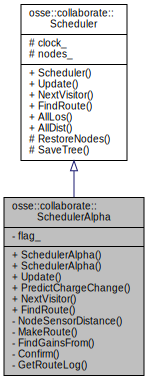
\includegraphics[width=220pt]{classosse_1_1collaborate_1_1_scheduler_alpha__inherit__graph}
\end{center}
\end{figure}
\subsubsection*{Public Member Functions}
\begin{DoxyCompactItemize}
\item 
\hyperlink{classosse_1_1collaborate_1_1_scheduler_alpha_abf962f131875a1091699fe16a4d0eeb8}{Scheduler\+Alpha} (\hyperlink{classosse_1_1collaborate_1_1_simulation_clock}{Simulation\+Clock} $\ast$\+\_\+clock)
\begin{DoxyCompactList}\small\item\em Constructor. \end{DoxyCompactList}\item 
\hyperlink{classosse_1_1collaborate_1_1_scheduler_alpha_aa3604fc73769a5c09280588532728409}{Scheduler\+Alpha} (\hyperlink{classosse_1_1collaborate_1_1_simulation_clock}{Simulation\+Clock} $\ast$\+\_\+clock, const bool \&\+\_\+flag)
\begin{DoxyCompactList}\small\item\em Constructor. \end{DoxyCompactList}\item 
void \hyperlink{classosse_1_1collaborate_1_1_scheduler_alpha_a375c441e048ff73c2d97816d9c9cb29e}{Update} (const std\+::vector$<$ \hyperlink{classosse_1_1collaborate_1_1_node}{Node} $\ast$$>$ \&\+\_\+nodes, \hyperlink{classosse_1_1collaborate_1_1_event_logger}{Event\+Logger} $\ast$\+\_\+event\+\_\+log)
\begin{DoxyCompactList}\small\item\em Updates the list of nodes. \end{DoxyCompactList}\item 
void \hyperlink{classosse_1_1collaborate_1_1_scheduler_alpha_a78709b9ddc8f6dd9b380432f6deedbb1}{Predict\+Charge\+Change} (\hyperlink{classosse_1_1collaborate_1_1_sun}{Sun} $\ast$\+\_\+sun, \hyperlink{classosse_1_1collaborate_1_1_node}{Node} $\ast$\+\_\+node, const uint64\+\_\+t \&\+\_\+limit\+\_\+s)
\begin{DoxyCompactList}\small\item\em Predicts the times at which charge status will change. \end{DoxyCompactList}\item 
bool \hyperlink{classosse_1_1collaborate_1_1_scheduler_alpha_ab757ae48c70b3409beb483d977bd62f5}{Next\+Visitor} (const std\+::vector$<$ \hyperlink{classosse_1_1collaborate_1_1_geodetic}{Geodetic} $>$ \&\+\_\+destinations\+\_\+rad\+\_\+m, const uint16\+\_\+t \&\+\_\+sink\+\_\+constellation, \hyperlink{classosse_1_1collaborate_1_1_node}{Node} $\ast$$\ast$next\+\_\+visitor\+\_\+, uint64\+\_\+t $\ast$prediction\+\_\+s\+\_\+)
\begin{DoxyCompactList}\small\item\em Find the next node to visit a location, at future time (seconds) \end{DoxyCompactList}\item 
std\+::vector$<$ std\+::pair$<$ uint16\+\_\+t, uint64\+\_\+t $>$ $>$ \hyperlink{classosse_1_1collaborate_1_1_scheduler_alpha_abf3bad26233bb4a9094a0236bc380f8e}{Find\+Route} (const uint16\+\_\+t \&\+\_\+start, const uint16\+\_\+t \&\+\_\+end, const uint64\+\_\+t \&\+\_\+contact\+\_\+s, const uint64\+\_\+t \&\+\_\+limit\+\_\+s)
\begin{DoxyCompactList}\small\item\em Constructs the most efficient time-\/dynamic route available. \end{DoxyCompactList}\end{DoxyCompactItemize}
\subsubsection*{Private Member Functions}
\begin{DoxyCompactItemize}
\item 
double \hyperlink{classosse_1_1collaborate_1_1_scheduler_alpha_a3347ebdec27431be3bbd389e1dad88a6}{Node\+Sensor\+Distance} (\hyperlink{classosse_1_1collaborate_1_1_node}{Node} $\ast$\+\_\+node, const \hyperlink{classosse_1_1collaborate_1_1_geodetic}{Geodetic} \&\+\_\+destination\+\_\+rad\+\_\+m, const uint64\+\_\+t \&\+\_\+offset\+\_\+s)
\begin{DoxyCompactList}\small\item\em Determines the distance from a sensor\textquotesingle{}s current reading position. \end{DoxyCompactList}\item 
std\+::vector$<$ std\+::pair$<$ uint16\+\_\+t, uint64\+\_\+t $>$ $>$ \hyperlink{classosse_1_1collaborate_1_1_scheduler_alpha_af858a8d223a945fd93235d0b68a44cee}{Make\+Route} (\hyperlink{classosse_1_1collaborate_1_1_tree}{Tree} $\ast$\+\_\+tree, const uint16\+\_\+t \&\+\_\+end, const uint64\+\_\+t \&\+\_\+contact\+\_\+s)
\begin{DoxyCompactList}\small\item\em Makes the route from the tree and adds it to the list. \end{DoxyCompactList}\item 
std\+::vector$<$ uint16\+\_\+t $>$ \hyperlink{classosse_1_1collaborate_1_1_scheduler_alpha_a6cf7cf015650e1837c6ae65bda26ff95}{Find\+Gains\+From} (const uint16\+\_\+t \&\+\_\+tx\+\_\+index, const uint64\+\_\+t \&\+\_\+offset\+\_\+s, const std\+::vector$<$ uint16\+\_\+t $>$ \&\+\_\+rxs)
\begin{DoxyCompactList}\small\item\em Finds the current open channels with neighbors. \end{DoxyCompactList}\item 
uint64\+\_\+t \hyperlink{classosse_1_1collaborate_1_1_scheduler_alpha_adc69d9527006a9eccc142f9369c93cb5}{Confirm} (\hyperlink{classosse_1_1collaborate_1_1_node}{Node} $\ast$\+\_\+tx\+\_\+node, \hyperlink{classosse_1_1collaborate_1_1_node}{Node} $\ast$\+\_\+rx\+\_\+node, const uint64\+\_\+t \&\+\_\+duration\+\_\+s, const uint64\+\_\+t \&\+\_\+original\+\_\+s, const uint64\+\_\+t \&\+\_\+lower\+\_\+limit\+\_\+s)
\begin{DoxyCompactList}\small\item\em Confirms that the contact lasts as long as the specified duration. \end{DoxyCompactList}\item 
std\+::string \hyperlink{classosse_1_1collaborate_1_1_scheduler_alpha_a66f56e307485a3ab62b625324006d945}{Get\+Route\+Log} (const uint16\+\_\+t \&\+\_\+start\+\_\+index, const std\+::vector$<$ std\+::pair$<$ uint16\+\_\+t, uint64\+\_\+t $>$$>$ \&\+\_\+route)
\begin{DoxyCompactList}\small\item\em Obtain the string log for the route. \end{DoxyCompactList}\end{DoxyCompactItemize}
\subsubsection*{Private Attributes}
\begin{DoxyCompactItemize}
\item 
\mbox{\Hypertarget{classosse_1_1collaborate_1_1_scheduler_alpha_a98ad63ff3f5454a21f08296db3d6fc6d}\label{classosse_1_1collaborate_1_1_scheduler_alpha_a98ad63ff3f5454a21f08296db3d6fc6d}} 
bool \hyperlink{classosse_1_1collaborate_1_1_scheduler_alpha_a98ad63ff3f5454a21f08296db3d6fc6d}{flag\+\_\+}
\begin{DoxyCompactList}\small\item\em Flag. \end{DoxyCompactList}\end{DoxyCompactItemize}
\subsubsection*{Additional Inherited Members}


\subsubsection{Detailed Description}
Concrete internal simulation processor. 

 
\begin{DoxyImageNoCaption}
  \mbox{\includegraphics[width=\textwidth]{collaborate}}
\end{DoxyImageNoCaption}
 

\subsubsection{Constructor \& Destructor Documentation}
\mbox{\Hypertarget{classosse_1_1collaborate_1_1_scheduler_alpha_abf962f131875a1091699fe16a4d0eeb8}\label{classosse_1_1collaborate_1_1_scheduler_alpha_abf962f131875a1091699fe16a4d0eeb8}} 
\index{osse\+::collaborate\+::\+Scheduler\+Alpha@{osse\+::collaborate\+::\+Scheduler\+Alpha}!Scheduler\+Alpha@{Scheduler\+Alpha}}
\index{Scheduler\+Alpha@{Scheduler\+Alpha}!osse\+::collaborate\+::\+Scheduler\+Alpha@{osse\+::collaborate\+::\+Scheduler\+Alpha}}
\paragraph{\texorpdfstring{Scheduler\+Alpha()}{SchedulerAlpha()}\hspace{0.1cm}{\footnotesize\ttfamily [1/2]}}
{\footnotesize\ttfamily osse\+::collaborate\+::\+Scheduler\+Alpha\+::\+Scheduler\+Alpha (\begin{DoxyParamCaption}\item[{\hyperlink{classosse_1_1collaborate_1_1_simulation_clock}{Simulation\+Clock} $\ast$}]{\+\_\+clock }\end{DoxyParamCaption})}



Constructor. 


\begin{DoxyParams}[1]{Parameters}
\mbox{\tt in}  & {\em \+\_\+clock} & Simulation clock \\
\hline
\end{DoxyParams}
\mbox{\Hypertarget{classosse_1_1collaborate_1_1_scheduler_alpha_aa3604fc73769a5c09280588532728409}\label{classosse_1_1collaborate_1_1_scheduler_alpha_aa3604fc73769a5c09280588532728409}} 
\index{osse\+::collaborate\+::\+Scheduler\+Alpha@{osse\+::collaborate\+::\+Scheduler\+Alpha}!Scheduler\+Alpha@{Scheduler\+Alpha}}
\index{Scheduler\+Alpha@{Scheduler\+Alpha}!osse\+::collaborate\+::\+Scheduler\+Alpha@{osse\+::collaborate\+::\+Scheduler\+Alpha}}
\paragraph{\texorpdfstring{Scheduler\+Alpha()}{SchedulerAlpha()}\hspace{0.1cm}{\footnotesize\ttfamily [2/2]}}
{\footnotesize\ttfamily osse\+::collaborate\+::\+Scheduler\+Alpha\+::\+Scheduler\+Alpha (\begin{DoxyParamCaption}\item[{\hyperlink{classosse_1_1collaborate_1_1_simulation_clock}{Simulation\+Clock} $\ast$}]{\+\_\+clock,  }\item[{const bool \&}]{\+\_\+flag }\end{DoxyParamCaption})}



Constructor. 


\begin{DoxyParams}[1]{Parameters}
\mbox{\tt in}  & {\em \+\_\+clock} & Simulation clock \\
\hline
\mbox{\tt in}  & {\em \+\_\+flag} & Flag \\
\hline
\end{DoxyParams}


\subsubsection{Member Function Documentation}
\mbox{\Hypertarget{classosse_1_1collaborate_1_1_scheduler_alpha_adc69d9527006a9eccc142f9369c93cb5}\label{classosse_1_1collaborate_1_1_scheduler_alpha_adc69d9527006a9eccc142f9369c93cb5}} 
\index{osse\+::collaborate\+::\+Scheduler\+Alpha@{osse\+::collaborate\+::\+Scheduler\+Alpha}!Confirm@{Confirm}}
\index{Confirm@{Confirm}!osse\+::collaborate\+::\+Scheduler\+Alpha@{osse\+::collaborate\+::\+Scheduler\+Alpha}}
\paragraph{\texorpdfstring{Confirm()}{Confirm()}}
{\footnotesize\ttfamily uint64\+\_\+t osse\+::collaborate\+::\+Scheduler\+Alpha\+::\+Confirm (\begin{DoxyParamCaption}\item[{\hyperlink{classosse_1_1collaborate_1_1_node}{Node} $\ast$}]{\+\_\+tx\+\_\+node,  }\item[{\hyperlink{classosse_1_1collaborate_1_1_node}{Node} $\ast$}]{\+\_\+rx\+\_\+node,  }\item[{const uint64\+\_\+t \&}]{\+\_\+duration\+\_\+s,  }\item[{const uint64\+\_\+t \&}]{\+\_\+original\+\_\+s,  }\item[{const uint64\+\_\+t \&}]{\+\_\+lower\+\_\+limit\+\_\+s }\end{DoxyParamCaption})\hspace{0.3cm}{\ttfamily [private]}}



Confirms that the contact lasts as long as the specified duration. 


\begin{DoxyParams}[1]{Parameters}
\mbox{\tt in}  & {\em \+\_\+tx\+\_\+node} & The transmitter \\
\hline
\mbox{\tt in}  & {\em \+\_\+rx\+\_\+node} & The receiver \\
\hline
\mbox{\tt in}  & {\em \+\_\+duration\+\_\+s} & The duration of contact (seconds) \\
\hline
\mbox{\tt in}  & {\em \+\_\+original\+\_\+s} & The starting offset (seconds) \\
\hline
\mbox{\tt in}  & {\em \+\_\+lower\+\_\+limit\+\_\+s} & The lower limit (seconds) \\
\hline
\end{DoxyParams}
\begin{DoxyReturn}{Returns}
The starting time of contact, or infinity if none found 
\end{DoxyReturn}
\mbox{\Hypertarget{classosse_1_1collaborate_1_1_scheduler_alpha_a6cf7cf015650e1837c6ae65bda26ff95}\label{classosse_1_1collaborate_1_1_scheduler_alpha_a6cf7cf015650e1837c6ae65bda26ff95}} 
\index{osse\+::collaborate\+::\+Scheduler\+Alpha@{osse\+::collaborate\+::\+Scheduler\+Alpha}!Find\+Gains\+From@{Find\+Gains\+From}}
\index{Find\+Gains\+From@{Find\+Gains\+From}!osse\+::collaborate\+::\+Scheduler\+Alpha@{osse\+::collaborate\+::\+Scheduler\+Alpha}}
\paragraph{\texorpdfstring{Find\+Gains\+From()}{FindGainsFrom()}}
{\footnotesize\ttfamily std\+::vector$<$ uint16\+\_\+t $>$ osse\+::collaborate\+::\+Scheduler\+Alpha\+::\+Find\+Gains\+From (\begin{DoxyParamCaption}\item[{const uint16\+\_\+t \&}]{\+\_\+tx\+\_\+index,  }\item[{const uint64\+\_\+t \&}]{\+\_\+offset\+\_\+s,  }\item[{const std\+::vector$<$ uint16\+\_\+t $>$ \&}]{\+\_\+rxs }\end{DoxyParamCaption})\hspace{0.3cm}{\ttfamily [private]}}



Finds the current open channels with neighbors. 


\begin{DoxyParams}[1]{Parameters}
\mbox{\tt in}  & {\em \+\_\+tx\+\_\+index} & The index of the transmitter \\
\hline
\mbox{\tt in}  & {\em \+\_\+offset\+\_\+s} & The time offset from current time (seconds) \\
\hline
\mbox{\tt in}  & {\em \+\_\+rxs} & The receivers to consider \\
\hline
\end{DoxyParams}
\begin{DoxyReturn}{Returns}
The possible receivers 
\end{DoxyReturn}
\mbox{\Hypertarget{classosse_1_1collaborate_1_1_scheduler_alpha_abf3bad26233bb4a9094a0236bc380f8e}\label{classosse_1_1collaborate_1_1_scheduler_alpha_abf3bad26233bb4a9094a0236bc380f8e}} 
\index{osse\+::collaborate\+::\+Scheduler\+Alpha@{osse\+::collaborate\+::\+Scheduler\+Alpha}!Find\+Route@{Find\+Route}}
\index{Find\+Route@{Find\+Route}!osse\+::collaborate\+::\+Scheduler\+Alpha@{osse\+::collaborate\+::\+Scheduler\+Alpha}}
\paragraph{\texorpdfstring{Find\+Route()}{FindRoute()}}
{\footnotesize\ttfamily std\+::vector$<$ std\+::pair$<$ uint16\+\_\+t, uint64\+\_\+t $>$ $>$ osse\+::collaborate\+::\+Scheduler\+Alpha\+::\+Find\+Route (\begin{DoxyParamCaption}\item[{const uint16\+\_\+t \&}]{\+\_\+start,  }\item[{const uint16\+\_\+t \&}]{\+\_\+end,  }\item[{const uint64\+\_\+t \&}]{\+\_\+contact\+\_\+s,  }\item[{const uint64\+\_\+t \&}]{\+\_\+limit\+\_\+s }\end{DoxyParamCaption})\hspace{0.3cm}{\ttfamily [virtual]}}



Constructs the most efficient time-\/dynamic route available. 


\begin{DoxyParams}[1]{Parameters}
\mbox{\tt in}  & {\em \+\_\+start} & Start node index \\
\hline
\mbox{\tt in}  & {\em \+\_\+end} & End node index \\
\hline
\mbox{\tt in}  & {\em \+\_\+contact\+\_\+s} & Duration of contact (seconds) \\
\hline
\mbox{\tt in}  & {\em \+\_\+limit\+\_\+s} & Expiration time limit (seconds) \\
\hline
\end{DoxyParams}
\begin{DoxyReturn}{Returns}
Most efficient time-\/dynamic route available 
\end{DoxyReturn}


Implements \hyperlink{classosse_1_1collaborate_1_1_scheduler_a060f7f9e1d09ca22cb43ded4b3c5d10c}{osse\+::collaborate\+::\+Scheduler}.

\mbox{\Hypertarget{classosse_1_1collaborate_1_1_scheduler_alpha_a66f56e307485a3ab62b625324006d945}\label{classosse_1_1collaborate_1_1_scheduler_alpha_a66f56e307485a3ab62b625324006d945}} 
\index{osse\+::collaborate\+::\+Scheduler\+Alpha@{osse\+::collaborate\+::\+Scheduler\+Alpha}!Get\+Route\+Log@{Get\+Route\+Log}}
\index{Get\+Route\+Log@{Get\+Route\+Log}!osse\+::collaborate\+::\+Scheduler\+Alpha@{osse\+::collaborate\+::\+Scheduler\+Alpha}}
\paragraph{\texorpdfstring{Get\+Route\+Log()}{GetRouteLog()}}
{\footnotesize\ttfamily std\+::string osse\+::collaborate\+::\+Scheduler\+Alpha\+::\+Get\+Route\+Log (\begin{DoxyParamCaption}\item[{const uint16\+\_\+t \&}]{\+\_\+start\+\_\+index,  }\item[{const std\+::vector$<$ std\+::pair$<$ uint16\+\_\+t, uint64\+\_\+t $>$$>$ \&}]{\+\_\+route }\end{DoxyParamCaption})\hspace{0.3cm}{\ttfamily [private]}}



Obtain the string log for the route. 


\begin{DoxyParams}[1]{Parameters}
\mbox{\tt in}  & {\em \+\_\+start\+\_\+index} & Starting node index \\
\hline
\mbox{\tt in}  & {\em \+\_\+route} & List of individual transfers \\
\hline
\end{DoxyParams}
\begin{DoxyReturn}{Returns}
String log for the route 
\end{DoxyReturn}
\mbox{\Hypertarget{classosse_1_1collaborate_1_1_scheduler_alpha_af858a8d223a945fd93235d0b68a44cee}\label{classosse_1_1collaborate_1_1_scheduler_alpha_af858a8d223a945fd93235d0b68a44cee}} 
\index{osse\+::collaborate\+::\+Scheduler\+Alpha@{osse\+::collaborate\+::\+Scheduler\+Alpha}!Make\+Route@{Make\+Route}}
\index{Make\+Route@{Make\+Route}!osse\+::collaborate\+::\+Scheduler\+Alpha@{osse\+::collaborate\+::\+Scheduler\+Alpha}}
\paragraph{\texorpdfstring{Make\+Route()}{MakeRoute()}}
{\footnotesize\ttfamily std\+::vector$<$ std\+::pair$<$ uint16\+\_\+t, uint64\+\_\+t $>$ $>$ osse\+::collaborate\+::\+Scheduler\+Alpha\+::\+Make\+Route (\begin{DoxyParamCaption}\item[{\hyperlink{classosse_1_1collaborate_1_1_tree}{Tree} $\ast$}]{\+\_\+tree,  }\item[{const uint16\+\_\+t \&}]{\+\_\+end,  }\item[{const uint64\+\_\+t \&}]{\+\_\+contact\+\_\+s }\end{DoxyParamCaption})\hspace{0.3cm}{\ttfamily [private]}}



Makes the route from the tree and adds it to the list. 


\begin{DoxyParams}[1]{Parameters}
\mbox{\tt in}  & {\em \+\_\+tree} & \hyperlink{classosse_1_1collaborate_1_1_tree}{Tree} \\
\hline
\mbox{\tt in}  & {\em \+\_\+end} & End node index \\
\hline
\mbox{\tt in}  & {\em \+\_\+contact\+\_\+s} & Duration of contact (seconds) \\
\hline
\end{DoxyParams}
\begin{DoxyReturn}{Returns}
Route 
\end{DoxyReturn}
\mbox{\Hypertarget{classosse_1_1collaborate_1_1_scheduler_alpha_ab757ae48c70b3409beb483d977bd62f5}\label{classosse_1_1collaborate_1_1_scheduler_alpha_ab757ae48c70b3409beb483d977bd62f5}} 
\index{osse\+::collaborate\+::\+Scheduler\+Alpha@{osse\+::collaborate\+::\+Scheduler\+Alpha}!Next\+Visitor@{Next\+Visitor}}
\index{Next\+Visitor@{Next\+Visitor}!osse\+::collaborate\+::\+Scheduler\+Alpha@{osse\+::collaborate\+::\+Scheduler\+Alpha}}
\paragraph{\texorpdfstring{Next\+Visitor()}{NextVisitor()}}
{\footnotesize\ttfamily bool osse\+::collaborate\+::\+Scheduler\+Alpha\+::\+Next\+Visitor (\begin{DoxyParamCaption}\item[{const std\+::vector$<$ \hyperlink{classosse_1_1collaborate_1_1_geodetic}{Geodetic} $>$ \&}]{\+\_\+destinations\+\_\+rad\+\_\+m,  }\item[{const uint16\+\_\+t \&}]{\+\_\+sink\+\_\+constellation,  }\item[{\hyperlink{classosse_1_1collaborate_1_1_node}{Node} $\ast$$\ast$}]{next\+\_\+visitor\+\_\+,  }\item[{uint64\+\_\+t $\ast$}]{prediction\+\_\+s\+\_\+ }\end{DoxyParamCaption})\hspace{0.3cm}{\ttfamily [virtual]}}



Find the next node to visit a location, at future time (seconds) 


\begin{DoxyParams}[1]{Parameters}
\mbox{\tt in}  & {\em \+\_\+destinations\+\_\+rad\+\_\+m} & Destinations \\
\hline
\mbox{\tt in}  & {\em \+\_\+sink\+\_\+constellation} & Number of the sink constellation \\
\hline
\mbox{\tt out}  & {\em next\+\_\+visitor\+\_\+} & Next visitor \\
\hline
\mbox{\tt out}  & {\em prediction\+\_\+s\+\_\+} & Time of the next visit (seconds) \\
\hline
\end{DoxyParams}
\begin{DoxyReturn}{Returns}
Whether a visitor has been found (if outputs are valid) 
\end{DoxyReturn}


Implements \hyperlink{classosse_1_1collaborate_1_1_scheduler_ababb48a841ec1b4903b69e799e43babf}{osse\+::collaborate\+::\+Scheduler}.

\mbox{\Hypertarget{classosse_1_1collaborate_1_1_scheduler_alpha_a3347ebdec27431be3bbd389e1dad88a6}\label{classosse_1_1collaborate_1_1_scheduler_alpha_a3347ebdec27431be3bbd389e1dad88a6}} 
\index{osse\+::collaborate\+::\+Scheduler\+Alpha@{osse\+::collaborate\+::\+Scheduler\+Alpha}!Node\+Sensor\+Distance@{Node\+Sensor\+Distance}}
\index{Node\+Sensor\+Distance@{Node\+Sensor\+Distance}!osse\+::collaborate\+::\+Scheduler\+Alpha@{osse\+::collaborate\+::\+Scheduler\+Alpha}}
\paragraph{\texorpdfstring{Node\+Sensor\+Distance()}{NodeSensorDistance()}}
{\footnotesize\ttfamily double osse\+::collaborate\+::\+Scheduler\+Alpha\+::\+Node\+Sensor\+Distance (\begin{DoxyParamCaption}\item[{\hyperlink{classosse_1_1collaborate_1_1_node}{Node} $\ast$}]{\+\_\+node,  }\item[{const \hyperlink{classosse_1_1collaborate_1_1_geodetic}{Geodetic} \&}]{\+\_\+destination\+\_\+rad\+\_\+m,  }\item[{const uint64\+\_\+t \&}]{\+\_\+offset\+\_\+s }\end{DoxyParamCaption})\hspace{0.3cm}{\ttfamily [private]}}



Determines the distance from a sensor\textquotesingle{}s current reading position. 


\begin{DoxyParams}[1]{Parameters}
\mbox{\tt in}  & {\em \+\_\+node} & \hyperlink{classosse_1_1collaborate_1_1_node}{Node} \\
\hline
\mbox{\tt in}  & {\em \+\_\+destination\+\_\+rad\+\_\+m} & \hyperlink{classosse_1_1collaborate_1_1_geodetic}{Geodetic} destination \\
\hline
\mbox{\tt in}  & {\em \+\_\+offset\+\_\+s} & Time offset from present (seconds) \\
\hline
\end{DoxyParams}
\begin{DoxyReturn}{Returns}
Distance from a sensor\textquotesingle{}s current reading position 
\end{DoxyReturn}
\mbox{\Hypertarget{classosse_1_1collaborate_1_1_scheduler_alpha_a78709b9ddc8f6dd9b380432f6deedbb1}\label{classosse_1_1collaborate_1_1_scheduler_alpha_a78709b9ddc8f6dd9b380432f6deedbb1}} 
\index{osse\+::collaborate\+::\+Scheduler\+Alpha@{osse\+::collaborate\+::\+Scheduler\+Alpha}!Predict\+Charge\+Change@{Predict\+Charge\+Change}}
\index{Predict\+Charge\+Change@{Predict\+Charge\+Change}!osse\+::collaborate\+::\+Scheduler\+Alpha@{osse\+::collaborate\+::\+Scheduler\+Alpha}}
\paragraph{\texorpdfstring{Predict\+Charge\+Change()}{PredictChargeChange()}}
{\footnotesize\ttfamily void osse\+::collaborate\+::\+Scheduler\+Alpha\+::\+Predict\+Charge\+Change (\begin{DoxyParamCaption}\item[{\hyperlink{classosse_1_1collaborate_1_1_sun}{Sun} $\ast$}]{\+\_\+sun,  }\item[{\hyperlink{classosse_1_1collaborate_1_1_node}{Node} $\ast$}]{\+\_\+node,  }\item[{const uint64\+\_\+t \&}]{\+\_\+limit\+\_\+s }\end{DoxyParamCaption})}



Predicts the times at which charge status will change. 


\begin{DoxyParams}[1]{Parameters}
\mbox{\tt in}  & {\em \+\_\+sun} & \hyperlink{classosse_1_1collaborate_1_1_sun}{Sun} \\
\hline
\mbox{\tt in}  & {\em \+\_\+node} & Subject node \\
\hline
\mbox{\tt in}  & {\em \+\_\+limit\+\_\+s} & Time limit (seconds) \\
\hline
\end{DoxyParams}
\mbox{\Hypertarget{classosse_1_1collaborate_1_1_scheduler_alpha_a375c441e048ff73c2d97816d9c9cb29e}\label{classosse_1_1collaborate_1_1_scheduler_alpha_a375c441e048ff73c2d97816d9c9cb29e}} 
\index{osse\+::collaborate\+::\+Scheduler\+Alpha@{osse\+::collaborate\+::\+Scheduler\+Alpha}!Update@{Update}}
\index{Update@{Update}!osse\+::collaborate\+::\+Scheduler\+Alpha@{osse\+::collaborate\+::\+Scheduler\+Alpha}}
\paragraph{\texorpdfstring{Update()}{Update()}}
{\footnotesize\ttfamily void osse\+::collaborate\+::\+Scheduler\+Alpha\+::\+Update (\begin{DoxyParamCaption}\item[{const std\+::vector$<$ \hyperlink{classosse_1_1collaborate_1_1_node}{Node} $\ast$$>$ \&}]{\+\_\+nodes,  }\item[{\hyperlink{classosse_1_1collaborate_1_1_event_logger}{Event\+Logger} $\ast$}]{\+\_\+event\+\_\+log }\end{DoxyParamCaption})\hspace{0.3cm}{\ttfamily [virtual]}}



Updates the list of nodes. 


\begin{DoxyParams}[1]{Parameters}
\mbox{\tt in}  & {\em \+\_\+nodes} & Nodes \\
\hline
\mbox{\tt in}  & {\em \+\_\+event\+\_\+log} & Event logger \\
\hline
\end{DoxyParams}


Implements \hyperlink{classosse_1_1collaborate_1_1_scheduler_a84241d85d4b53716d3918f44c56875b2}{osse\+::collaborate\+::\+Scheduler}.



The documentation for this class was generated from the following files\+:\begin{DoxyCompactItemize}
\item 
libs/collaborate/include/collaborate/scheduler\+\_\+alpha.\+h\item 
libs/collaborate/src/scheduler\+\_\+alpha.\+cpp\end{DoxyCompactItemize}

\hypertarget{classosse_1_1collaborate_1_1_scheduler}{}\subsection{osse\+:\+:collaborate\+:\+:Scheduler Class Reference}
\label{classosse_1_1collaborate_1_1_scheduler}\index{osse\+::collaborate\+::\+Scheduler@{osse\+::collaborate\+::\+Scheduler}}


Abstract internal simulation processor.  




{\ttfamily \#include $<$scheduler.\+h$>$}



Inheritance diagram for osse\+:\+:collaborate\+:\+:Scheduler\+:
\nopagebreak
\begin{figure}[H]
\begin{center}
\leavevmode
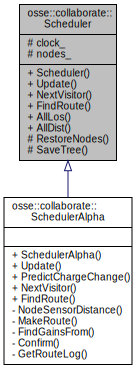
\includegraphics[width=220pt]{classosse_1_1collaborate_1_1_scheduler__inherit__graph}
\end{center}
\end{figure}
\subsubsection*{Public Member Functions}
\begin{DoxyCompactItemize}
\item 
\hyperlink{classosse_1_1collaborate_1_1_scheduler_a7052cb2998cbcce276e1c0b45b5aaa6a}{Scheduler} (\hyperlink{classosse_1_1collaborate_1_1_simulation_clock}{Simulation\+Clock} $\ast$\+\_\+clock)
\begin{DoxyCompactList}\small\item\em Constructor. \end{DoxyCompactList}\item 
virtual void \hyperlink{classosse_1_1collaborate_1_1_scheduler_a84241d85d4b53716d3918f44c56875b2}{Update} (const std\+::vector$<$ \hyperlink{classosse_1_1collaborate_1_1_node}{Node} $\ast$$>$ \&\+\_\+nodes, \hyperlink{classosse_1_1collaborate_1_1_event_logger}{Event\+Logger} $\ast$\+\_\+event\+\_\+log)=0
\begin{DoxyCompactList}\small\item\em Runs the scheduling algorithm. \end{DoxyCompactList}\item 
virtual bool \hyperlink{classosse_1_1collaborate_1_1_scheduler_ababb48a841ec1b4903b69e799e43babf}{Next\+Visitor} (const std\+::vector$<$ \hyperlink{classosse_1_1collaborate_1_1_geodetic}{Geodetic} $>$ \&\+\_\+destinations\+\_\+rad\+\_\+m, const uint16\+\_\+t \&\+\_\+sink\+\_\+constellation, \hyperlink{classosse_1_1collaborate_1_1_node}{Node} $\ast$$\ast$next\+\_\+visitor\+\_\+, uint64\+\_\+t $\ast$prediction\+\_\+s\+\_\+)=0
\begin{DoxyCompactList}\small\item\em Find the next node to visit a location, at future time (seconds) \end{DoxyCompactList}\item 
virtual std\+::vector$<$ std\+::pair$<$ uint16\+\_\+t, uint64\+\_\+t $>$ $>$ \hyperlink{classosse_1_1collaborate_1_1_scheduler_a060f7f9e1d09ca22cb43ded4b3c5d10c}{Find\+Route} (const uint16\+\_\+t \&\+\_\+start, const uint16\+\_\+t \&\+\_\+end, const uint64\+\_\+t \&\+\_\+contact\+\_\+s, const uint64\+\_\+t \&\+\_\+limit\+\_\+s)=0
\begin{DoxyCompactList}\small\item\em Constructs the most efficient time-\/dynamic route available. \end{DoxyCompactList}\item 
void \hyperlink{classosse_1_1collaborate_1_1_scheduler_aab675402de557bac32d7cfc71aaf45b0}{All\+Los} (\hyperlink{classosse_1_1collaborate_1_1_graph_unweighted}{Graph\+Unweighted} $\ast$\+\_\+unweighted)
\begin{DoxyCompactList}\small\item\em Fills the unweighted graph with L\+OS connections. \end{DoxyCompactList}\item 
void \hyperlink{classosse_1_1collaborate_1_1_scheduler_a8dbb2201286d8c4f064cd1371d60ca90}{All\+Dist} (\hyperlink{classosse_1_1collaborate_1_1_graph_weighted}{Graph\+Weighted} $\ast$\+\_\+weighted)
\begin{DoxyCompactList}\small\item\em Fills the weighted graph with distances. \end{DoxyCompactList}\end{DoxyCompactItemize}
\subsubsection*{Protected Member Functions}
\begin{DoxyCompactItemize}
\item 
\mbox{\Hypertarget{classosse_1_1collaborate_1_1_scheduler_a96b4b7064d05318493a95185cc41c478}\label{classosse_1_1collaborate_1_1_scheduler_a96b4b7064d05318493a95185cc41c478}} 
void \hyperlink{classosse_1_1collaborate_1_1_scheduler_a96b4b7064d05318493a95185cc41c478}{Restore\+Nodes} ()
\begin{DoxyCompactList}\small\item\em Restores all nodes to original orbital\+\_\+state. \end{DoxyCompactList}\item 
void \hyperlink{classosse_1_1collaborate_1_1_scheduler_af4731ceeb474f42e800d0683b2a9bfc8}{Save\+Tree} (const uint16\+\_\+t \&\+\_\+start, const uint16\+\_\+t \&\+\_\+end, const \hyperlink{classosse_1_1collaborate_1_1_tree}{Tree} \&\+\_\+tree)
\begin{DoxyCompactList}\small\item\em Saves a tree to a text file. \end{DoxyCompactList}\end{DoxyCompactItemize}
\subsubsection*{Protected Attributes}
\begin{DoxyCompactItemize}
\item 
\mbox{\Hypertarget{classosse_1_1collaborate_1_1_scheduler_ac1f31c1dbf1db5ad65e9bc04a0fad031}\label{classosse_1_1collaborate_1_1_scheduler_ac1f31c1dbf1db5ad65e9bc04a0fad031}} 
\hyperlink{classosse_1_1collaborate_1_1_simulation_clock}{Simulation\+Clock} $\ast$ \hyperlink{classosse_1_1collaborate_1_1_scheduler_ac1f31c1dbf1db5ad65e9bc04a0fad031}{clock\+\_\+}
\begin{DoxyCompactList}\small\item\em Simulation clock. \end{DoxyCompactList}\item 
\mbox{\Hypertarget{classosse_1_1collaborate_1_1_scheduler_a1b7f83b7ec18fe151bd52c6b8a066542}\label{classosse_1_1collaborate_1_1_scheduler_a1b7f83b7ec18fe151bd52c6b8a066542}} 
std\+::vector$<$ \hyperlink{classosse_1_1collaborate_1_1_node}{Node} $\ast$ $>$ \hyperlink{classosse_1_1collaborate_1_1_scheduler_a1b7f83b7ec18fe151bd52c6b8a066542}{nodes\+\_\+}
\begin{DoxyCompactList}\small\item\em Current nodes from sensor network. \end{DoxyCompactList}\end{DoxyCompactItemize}


\subsubsection{Detailed Description}
Abstract internal simulation processor. 

\subsubsection{Constructor \& Destructor Documentation}
\mbox{\Hypertarget{classosse_1_1collaborate_1_1_scheduler_a7052cb2998cbcce276e1c0b45b5aaa6a}\label{classosse_1_1collaborate_1_1_scheduler_a7052cb2998cbcce276e1c0b45b5aaa6a}} 
\index{osse\+::collaborate\+::\+Scheduler@{osse\+::collaborate\+::\+Scheduler}!Scheduler@{Scheduler}}
\index{Scheduler@{Scheduler}!osse\+::collaborate\+::\+Scheduler@{osse\+::collaborate\+::\+Scheduler}}
\paragraph{\texorpdfstring{Scheduler()}{Scheduler()}}
{\footnotesize\ttfamily osse\+::collaborate\+::\+Scheduler\+::\+Scheduler (\begin{DoxyParamCaption}\item[{\hyperlink{classosse_1_1collaborate_1_1_simulation_clock}{Simulation\+Clock} $\ast$}]{\+\_\+clock }\end{DoxyParamCaption})\hspace{0.3cm}{\ttfamily [explicit]}}



Constructor. 


\begin{DoxyParams}[1]{Parameters}
\mbox{\tt in}  & {\em \+\_\+clock} & Simulation clock \\
\hline
\end{DoxyParams}


\subsubsection{Member Function Documentation}
\mbox{\Hypertarget{classosse_1_1collaborate_1_1_scheduler_a8dbb2201286d8c4f064cd1371d60ca90}\label{classosse_1_1collaborate_1_1_scheduler_a8dbb2201286d8c4f064cd1371d60ca90}} 
\index{osse\+::collaborate\+::\+Scheduler@{osse\+::collaborate\+::\+Scheduler}!All\+Dist@{All\+Dist}}
\index{All\+Dist@{All\+Dist}!osse\+::collaborate\+::\+Scheduler@{osse\+::collaborate\+::\+Scheduler}}
\paragraph{\texorpdfstring{All\+Dist()}{AllDist()}}
{\footnotesize\ttfamily void osse\+::collaborate\+::\+Scheduler\+::\+All\+Dist (\begin{DoxyParamCaption}\item[{\hyperlink{classosse_1_1collaborate_1_1_graph_weighted}{Graph\+Weighted} $\ast$}]{\+\_\+weighted }\end{DoxyParamCaption})}



Fills the weighted graph with distances. 


\begin{DoxyParams}[1]{Parameters}
\mbox{\tt in}  & {\em \+\_\+weighted} & Weighted graph \\
\hline
\end{DoxyParams}
\mbox{\Hypertarget{classosse_1_1collaborate_1_1_scheduler_aab675402de557bac32d7cfc71aaf45b0}\label{classosse_1_1collaborate_1_1_scheduler_aab675402de557bac32d7cfc71aaf45b0}} 
\index{osse\+::collaborate\+::\+Scheduler@{osse\+::collaborate\+::\+Scheduler}!All\+Los@{All\+Los}}
\index{All\+Los@{All\+Los}!osse\+::collaborate\+::\+Scheduler@{osse\+::collaborate\+::\+Scheduler}}
\paragraph{\texorpdfstring{All\+Los()}{AllLos()}}
{\footnotesize\ttfamily void osse\+::collaborate\+::\+Scheduler\+::\+All\+Los (\begin{DoxyParamCaption}\item[{\hyperlink{classosse_1_1collaborate_1_1_graph_unweighted}{Graph\+Unweighted} $\ast$}]{\+\_\+unweighted }\end{DoxyParamCaption})}



Fills the unweighted graph with L\+OS connections. 


\begin{DoxyParams}[1]{Parameters}
\mbox{\tt in}  & {\em \+\_\+unweighted} & Unweighted graph \\
\hline
\end{DoxyParams}
\mbox{\Hypertarget{classosse_1_1collaborate_1_1_scheduler_a060f7f9e1d09ca22cb43ded4b3c5d10c}\label{classosse_1_1collaborate_1_1_scheduler_a060f7f9e1d09ca22cb43ded4b3c5d10c}} 
\index{osse\+::collaborate\+::\+Scheduler@{osse\+::collaborate\+::\+Scheduler}!Find\+Route@{Find\+Route}}
\index{Find\+Route@{Find\+Route}!osse\+::collaborate\+::\+Scheduler@{osse\+::collaborate\+::\+Scheduler}}
\paragraph{\texorpdfstring{Find\+Route()}{FindRoute()}}
{\footnotesize\ttfamily virtual std\+::vector$<$std\+::pair$<$uint16\+\_\+t, uint64\+\_\+t$>$ $>$ osse\+::collaborate\+::\+Scheduler\+::\+Find\+Route (\begin{DoxyParamCaption}\item[{const uint16\+\_\+t \&}]{\+\_\+start,  }\item[{const uint16\+\_\+t \&}]{\+\_\+end,  }\item[{const uint64\+\_\+t \&}]{\+\_\+contact\+\_\+s,  }\item[{const uint64\+\_\+t \&}]{\+\_\+limit\+\_\+s }\end{DoxyParamCaption})\hspace{0.3cm}{\ttfamily [pure virtual]}}



Constructs the most efficient time-\/dynamic route available. 


\begin{DoxyParams}[1]{Parameters}
\mbox{\tt in}  & {\em \+\_\+start} & Start node index \\
\hline
\mbox{\tt in}  & {\em \+\_\+end} & End node index \\
\hline
\mbox{\tt in}  & {\em \+\_\+contact\+\_\+s} & Duration of contact (seconds) \\
\hline
\mbox{\tt in}  & {\em \+\_\+limit\+\_\+s} & Expiration time limit (seconds) \\
\hline
\end{DoxyParams}
\begin{DoxyReturn}{Returns}
Most efficient time-\/dynamic route available 
\end{DoxyReturn}


Implemented in \hyperlink{classosse_1_1collaborate_1_1_scheduler_alpha_abf3bad26233bb4a9094a0236bc380f8e}{osse\+::collaborate\+::\+Scheduler\+Alpha}.

\mbox{\Hypertarget{classosse_1_1collaborate_1_1_scheduler_ababb48a841ec1b4903b69e799e43babf}\label{classosse_1_1collaborate_1_1_scheduler_ababb48a841ec1b4903b69e799e43babf}} 
\index{osse\+::collaborate\+::\+Scheduler@{osse\+::collaborate\+::\+Scheduler}!Next\+Visitor@{Next\+Visitor}}
\index{Next\+Visitor@{Next\+Visitor}!osse\+::collaborate\+::\+Scheduler@{osse\+::collaborate\+::\+Scheduler}}
\paragraph{\texorpdfstring{Next\+Visitor()}{NextVisitor()}}
{\footnotesize\ttfamily virtual bool osse\+::collaborate\+::\+Scheduler\+::\+Next\+Visitor (\begin{DoxyParamCaption}\item[{const std\+::vector$<$ \hyperlink{classosse_1_1collaborate_1_1_geodetic}{Geodetic} $>$ \&}]{\+\_\+destinations\+\_\+rad\+\_\+m,  }\item[{const uint16\+\_\+t \&}]{\+\_\+sink\+\_\+constellation,  }\item[{\hyperlink{classosse_1_1collaborate_1_1_node}{Node} $\ast$$\ast$}]{next\+\_\+visitor\+\_\+,  }\item[{uint64\+\_\+t $\ast$}]{prediction\+\_\+s\+\_\+ }\end{DoxyParamCaption})\hspace{0.3cm}{\ttfamily [pure virtual]}}



Find the next node to visit a location, at future time (seconds) 


\begin{DoxyParams}[1]{Parameters}
\mbox{\tt in}  & {\em \+\_\+destinations\+\_\+rad\+\_\+m} & Destinations (meters and radians) \\
\hline
\mbox{\tt in}  & {\em \+\_\+sink\+\_\+constellation} & Which constellation to track \\
\hline
\mbox{\tt out}  & {\em next\+\_\+visitor\+\_\+} & Next visitor \\
\hline
\mbox{\tt out}  & {\em prediction\+\_\+s\+\_\+} & Time of the next visit (seconds) \\
\hline
\end{DoxyParams}
\begin{DoxyReturn}{Returns}
Whether a visitor has been found (if outputs are valid) 
\end{DoxyReturn}


Implemented in \hyperlink{classosse_1_1collaborate_1_1_scheduler_alpha_ab757ae48c70b3409beb483d977bd62f5}{osse\+::collaborate\+::\+Scheduler\+Alpha}.

\mbox{\Hypertarget{classosse_1_1collaborate_1_1_scheduler_af4731ceeb474f42e800d0683b2a9bfc8}\label{classosse_1_1collaborate_1_1_scheduler_af4731ceeb474f42e800d0683b2a9bfc8}} 
\index{osse\+::collaborate\+::\+Scheduler@{osse\+::collaborate\+::\+Scheduler}!Save\+Tree@{Save\+Tree}}
\index{Save\+Tree@{Save\+Tree}!osse\+::collaborate\+::\+Scheduler@{osse\+::collaborate\+::\+Scheduler}}
\paragraph{\texorpdfstring{Save\+Tree()}{SaveTree()}}
{\footnotesize\ttfamily void osse\+::collaborate\+::\+Scheduler\+::\+Save\+Tree (\begin{DoxyParamCaption}\item[{const uint16\+\_\+t \&}]{\+\_\+start,  }\item[{const uint16\+\_\+t \&}]{\+\_\+end,  }\item[{const \hyperlink{classosse_1_1collaborate_1_1_tree}{Tree} \&}]{\+\_\+tree }\end{DoxyParamCaption})\hspace{0.3cm}{\ttfamily [protected]}}



Saves a tree to a text file. 


\begin{DoxyParams}[1]{Parameters}
\mbox{\tt in}  & {\em \+\_\+tree} & \hyperlink{classosse_1_1collaborate_1_1_tree}{Tree} \\
\hline
\mbox{\tt in}  & {\em \+\_\+start} & Start node index \\
\hline
\mbox{\tt in}  & {\em \+\_\+end} & End node index \\
\hline
\end{DoxyParams}
\mbox{\Hypertarget{classosse_1_1collaborate_1_1_scheduler_a84241d85d4b53716d3918f44c56875b2}\label{classosse_1_1collaborate_1_1_scheduler_a84241d85d4b53716d3918f44c56875b2}} 
\index{osse\+::collaborate\+::\+Scheduler@{osse\+::collaborate\+::\+Scheduler}!Update@{Update}}
\index{Update@{Update}!osse\+::collaborate\+::\+Scheduler@{osse\+::collaborate\+::\+Scheduler}}
\paragraph{\texorpdfstring{Update()}{Update()}}
{\footnotesize\ttfamily virtual void osse\+::collaborate\+::\+Scheduler\+::\+Update (\begin{DoxyParamCaption}\item[{const std\+::vector$<$ \hyperlink{classosse_1_1collaborate_1_1_node}{Node} $\ast$$>$ \&}]{\+\_\+nodes,  }\item[{\hyperlink{classosse_1_1collaborate_1_1_event_logger}{Event\+Logger} $\ast$}]{\+\_\+event\+\_\+log }\end{DoxyParamCaption})\hspace{0.3cm}{\ttfamily [pure virtual]}}



Runs the scheduling algorithm. 


\begin{DoxyParams}[1]{Parameters}
\mbox{\tt in}  & {\em \+\_\+nodes} & Nodes \\
\hline
\mbox{\tt in}  & {\em \+\_\+event\+\_\+log} & Event logger \\
\hline
\end{DoxyParams}


Implemented in \hyperlink{classosse_1_1collaborate_1_1_scheduler_alpha_a375c441e048ff73c2d97816d9c9cb29e}{osse\+::collaborate\+::\+Scheduler\+Alpha}.



The documentation for this class was generated from the following files\+:\begin{DoxyCompactItemize}
\item 
libs/collaborate/include/collaborate/scheduler.\+h\item 
libs/collaborate/src/scheduler.\+cpp\end{DoxyCompactItemize}

\hypertarget{classosse_1_1collaborate_1_1_sensor_cloud_radar}{}\subsection{osse\+:\+:collaborate\+:\+:Sensor\+Cloud\+Radar Class Reference}
\label{classosse_1_1collaborate_1_1_sensor_cloud_radar}\index{osse\+::collaborate\+::\+Sensor\+Cloud\+Radar@{osse\+::collaborate\+::\+Sensor\+Cloud\+Radar}}


Measures total cloud optical depth.  




{\ttfamily \#include $<$sensor\+\_\+cloud\+\_\+radar.\+h$>$}



Inheritance diagram for osse\+:\+:collaborate\+:\+:Sensor\+Cloud\+Radar\+:
\nopagebreak
\begin{figure}[H]
\begin{center}
\leavevmode
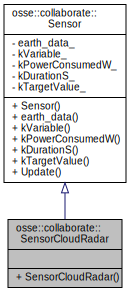
\includegraphics[width=213pt]{classosse_1_1collaborate_1_1_sensor_cloud_radar__inherit__graph}
\end{center}
\end{figure}
\subsubsection*{Public Member Functions}
\begin{DoxyCompactItemize}
\item 
\hyperlink{classosse_1_1collaborate_1_1_sensor_cloud_radar_aa23eab08fd54a881f9a85f1b35616386}{Sensor\+Cloud\+Radar} (const std\+::string \&\+\_\+path, const uint64\+\_\+t \&\+\_\+duration\+\_\+s)
\begin{DoxyCompactList}\small\item\em Constructor. \end{DoxyCompactList}\end{DoxyCompactItemize}


\subsubsection{Detailed Description}
Measures total cloud optical depth. 

\subsubsection{Constructor \& Destructor Documentation}
\mbox{\Hypertarget{classosse_1_1collaborate_1_1_sensor_cloud_radar_aa23eab08fd54a881f9a85f1b35616386}\label{classosse_1_1collaborate_1_1_sensor_cloud_radar_aa23eab08fd54a881f9a85f1b35616386}} 
\index{osse\+::collaborate\+::\+Sensor\+Cloud\+Radar@{osse\+::collaborate\+::\+Sensor\+Cloud\+Radar}!Sensor\+Cloud\+Radar@{Sensor\+Cloud\+Radar}}
\index{Sensor\+Cloud\+Radar@{Sensor\+Cloud\+Radar}!osse\+::collaborate\+::\+Sensor\+Cloud\+Radar@{osse\+::collaborate\+::\+Sensor\+Cloud\+Radar}}
\paragraph{\texorpdfstring{Sensor\+Cloud\+Radar()}{SensorCloudRadar()}}
{\footnotesize\ttfamily osse\+::collaborate\+::\+Sensor\+Cloud\+Radar\+::\+Sensor\+Cloud\+Radar (\begin{DoxyParamCaption}\item[{const std\+::string \&}]{\+\_\+path,  }\item[{const uint64\+\_\+t \&}]{\+\_\+duration\+\_\+s }\end{DoxyParamCaption})}



Constructor. 


\begin{DoxyParams}[1]{Parameters}
\mbox{\tt in}  & {\em \+\_\+path} & Parent directory path \\
\hline
\mbox{\tt in}  & {\em \+\_\+duration\+\_\+s} & Duration of measurements (seconds) \\
\hline
\end{DoxyParams}


The documentation for this class was generated from the following files\+:\begin{DoxyCompactItemize}
\item 
libs/collaborate/include/collaborate/sensor\+\_\+cloud\+\_\+radar.\+h\item 
libs/collaborate/src/sensor\+\_\+cloud\+\_\+radar.\+cpp\end{DoxyCompactItemize}

\hypertarget{classosse_1_1collaborate_1_1_sensor_optical_imager}{}\subsection{osse\+:\+:collaborate\+:\+:Sensor\+Optical\+Imager Class Reference}
\label{classosse_1_1collaborate_1_1_sensor_optical_imager}\index{osse\+::collaborate\+::\+Sensor\+Optical\+Imager@{osse\+::collaborate\+::\+Sensor\+Optical\+Imager}}


Obtains optical images of Earth\textquotesingle{}s surface.  




{\ttfamily \#include $<$sensor\+\_\+optical\+\_\+imager.\+h$>$}



Inheritance diagram for osse\+:\+:collaborate\+:\+:Sensor\+Optical\+Imager\+:
\nopagebreak
\begin{figure}[H]
\begin{center}
\leavevmode
\includegraphics[width=217pt]{classosse_1_1collaborate_1_1_sensor_optical_imager__inherit__graph}
\end{center}
\end{figure}
\subsubsection*{Public Member Functions}
\begin{DoxyCompactItemize}
\item 
\hyperlink{classosse_1_1collaborate_1_1_sensor_optical_imager_adee811f8926a698d9a56815742575259}{Sensor\+Optical\+Imager} (const std\+::string \&\+\_\+path, const uint64\+\_\+t \&\+\_\+duration\+\_\+s)
\begin{DoxyCompactList}\small\item\em Constructor. \end{DoxyCompactList}\end{DoxyCompactItemize}


\subsubsection{Detailed Description}
Obtains optical images of Earth\textquotesingle{}s surface. 

\subsubsection{Constructor \& Destructor Documentation}
\mbox{\Hypertarget{classosse_1_1collaborate_1_1_sensor_optical_imager_adee811f8926a698d9a56815742575259}\label{classosse_1_1collaborate_1_1_sensor_optical_imager_adee811f8926a698d9a56815742575259}} 
\index{osse\+::collaborate\+::\+Sensor\+Optical\+Imager@{osse\+::collaborate\+::\+Sensor\+Optical\+Imager}!Sensor\+Optical\+Imager@{Sensor\+Optical\+Imager}}
\index{Sensor\+Optical\+Imager@{Sensor\+Optical\+Imager}!osse\+::collaborate\+::\+Sensor\+Optical\+Imager@{osse\+::collaborate\+::\+Sensor\+Optical\+Imager}}
\paragraph{\texorpdfstring{Sensor\+Optical\+Imager()}{SensorOpticalImager()}}
{\footnotesize\ttfamily osse\+::collaborate\+::\+Sensor\+Optical\+Imager\+::\+Sensor\+Optical\+Imager (\begin{DoxyParamCaption}\item[{const std\+::string \&}]{\+\_\+path,  }\item[{const uint64\+\_\+t \&}]{\+\_\+duration\+\_\+s }\end{DoxyParamCaption})}



Constructor. 


\begin{DoxyParams}[1]{Parameters}
\mbox{\tt in}  & {\em \+\_\+path} & Parent directory path \\
\hline
\mbox{\tt in}  & {\em \+\_\+duration\+\_\+s} & Duration of measurements (seconds) \\
\hline
\end{DoxyParams}


The documentation for this class was generated from the following files\+:\begin{DoxyCompactItemize}
\item 
libs/collaborate/include/collaborate/sensor\+\_\+optical\+\_\+imager.\+h\item 
libs/collaborate/src/sensor\+\_\+optical\+\_\+imager.\+cpp\end{DoxyCompactItemize}

\hypertarget{classosse_1_1collaborate_1_1_sensor_rain_radar}{}\subsection{osse\+:\+:collaborate\+:\+:Sensor\+Rain\+Radar Class Reference}
\label{classosse_1_1collaborate_1_1_sensor_rain_radar}\index{osse\+::collaborate\+::\+Sensor\+Rain\+Radar@{osse\+::collaborate\+::\+Sensor\+Rain\+Radar}}


Measures total precipitation.  




{\ttfamily \#include $<$sensor\+\_\+rain\+\_\+radar.\+h$>$}



Inheritance diagram for osse\+:\+:collaborate\+:\+:Sensor\+Rain\+Radar\+:
\nopagebreak
\begin{figure}[H]
\begin{center}
\leavevmode
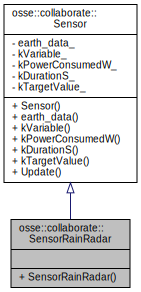
\includegraphics[width=213pt]{classosse_1_1collaborate_1_1_sensor_rain_radar__inherit__graph}
\end{center}
\end{figure}
\subsubsection*{Public Member Functions}
\begin{DoxyCompactItemize}
\item 
\hyperlink{classosse_1_1collaborate_1_1_sensor_rain_radar_af454a12a4cfea3b84b9c0901c9088e2d}{Sensor\+Rain\+Radar} (const std\+::string \&\+\_\+path, const uint64\+\_\+t \&\+\_\+duration\+\_\+s)
\begin{DoxyCompactList}\small\item\em Constructor. \end{DoxyCompactList}\end{DoxyCompactItemize}


\subsubsection{Detailed Description}
Measures total precipitation. 

\subsubsection{Constructor \& Destructor Documentation}
\mbox{\Hypertarget{classosse_1_1collaborate_1_1_sensor_rain_radar_af454a12a4cfea3b84b9c0901c9088e2d}\label{classosse_1_1collaborate_1_1_sensor_rain_radar_af454a12a4cfea3b84b9c0901c9088e2d}} 
\index{osse\+::collaborate\+::\+Sensor\+Rain\+Radar@{osse\+::collaborate\+::\+Sensor\+Rain\+Radar}!Sensor\+Rain\+Radar@{Sensor\+Rain\+Radar}}
\index{Sensor\+Rain\+Radar@{Sensor\+Rain\+Radar}!osse\+::collaborate\+::\+Sensor\+Rain\+Radar@{osse\+::collaborate\+::\+Sensor\+Rain\+Radar}}
\paragraph{\texorpdfstring{Sensor\+Rain\+Radar()}{SensorRainRadar()}}
{\footnotesize\ttfamily osse\+::collaborate\+::\+Sensor\+Rain\+Radar\+::\+Sensor\+Rain\+Radar (\begin{DoxyParamCaption}\item[{const std\+::string \&}]{\+\_\+path,  }\item[{const uint64\+\_\+t \&}]{\+\_\+duration\+\_\+s }\end{DoxyParamCaption})}



Constructor. 


\begin{DoxyParams}[1]{Parameters}
\mbox{\tt in}  & {\em \+\_\+path} & Parent directory path \\
\hline
\mbox{\tt in}  & {\em \+\_\+duration\+\_\+s} & Duration of measurements (seconds) \\
\hline
\end{DoxyParams}


The documentation for this class was generated from the following files\+:\begin{DoxyCompactItemize}
\item 
libs/collaborate/include/collaborate/sensor\+\_\+rain\+\_\+radar.\+h\item 
libs/collaborate/src/sensor\+\_\+rain\+\_\+radar.\+cpp\end{DoxyCompactItemize}

\hypertarget{classosse_1_1collaborate_1_1_sensor}{}\subsection{osse\+:\+:collaborate\+:\+:Sensor Class Reference}
\label{classosse_1_1collaborate_1_1_sensor}\index{osse\+::collaborate\+::\+Sensor@{osse\+::collaborate\+::\+Sensor}}


Measures scientific data.  




{\ttfamily \#include $<$sensor.\+h$>$}



Inheritance diagram for osse\+:\+:collaborate\+:\+:Sensor\+:
\nopagebreak
\begin{figure}[H]
\begin{center}
\leavevmode
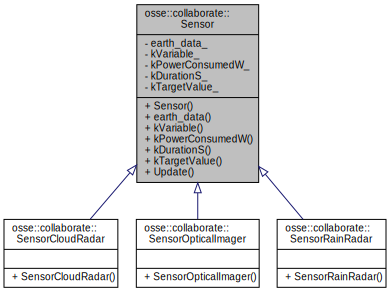
\includegraphics[width=350pt]{classosse_1_1collaborate_1_1_sensor__inherit__graph}
\end{center}
\end{figure}
\subsubsection*{Public Member Functions}
\begin{DoxyCompactItemize}
\item 
\hyperlink{classosse_1_1collaborate_1_1_sensor_a54618610f28a522fa48dd43ea4cdac9a}{Sensor} (\hyperlink{classosse_1_1collaborate_1_1_earth_data}{Earth\+Data} $\ast$\+\_\+earth\+\_\+data, const std\+::string \&\+\_\+variable, const double \&\+\_\+power\+\_\+consumed\+\_\+w, const uint64\+\_\+t \&\+\_\+duration\+\_\+s, const double \&\+\_\+target\+\_\+value)
\begin{DoxyCompactList}\small\item\em Constructor from earth\+\_\+data. \end{DoxyCompactList}\item 
\hyperlink{classosse_1_1collaborate_1_1_earth_data}{Earth\+Data} $\ast$ \hyperlink{classosse_1_1collaborate_1_1_sensor_a60ed2a55579dc999d9d4a40b4e2d2473}{earth\+\_\+data} () const
\begin{DoxyCompactList}\small\item\em Get The earth\+\_\+data of scientific data. \end{DoxyCompactList}\item 
const std\+::string \& \hyperlink{classosse_1_1collaborate_1_1_sensor_a06cf8b42c998b5125fcaef972f1950fd}{k\+Variable} () const
\begin{DoxyCompactList}\small\item\em Get variable name. \end{DoxyCompactList}\item 
const double \& \hyperlink{classosse_1_1collaborate_1_1_sensor_add78370d01a8feb5d1027a791906b691}{k\+Power\+ConsumedW} () const
\begin{DoxyCompactList}\small\item\em Get power consumed (Watts) \end{DoxyCompactList}\item 
const uint64\+\_\+t \& \hyperlink{classosse_1_1collaborate_1_1_sensor_a79da44f371358582b3ab820db6069614}{k\+DurationS} () const
\begin{DoxyCompactList}\small\item\em Get duration of measurements (seconds) \end{DoxyCompactList}\item 
const double \& \hyperlink{classosse_1_1collaborate_1_1_sensor_ae19c635fce562849ee3d1e7883bee22c}{k\+Target\+Value} () const
\begin{DoxyCompactList}\small\item\em Get target value for measurements. \end{DoxyCompactList}\item 
void \hyperlink{classosse_1_1collaborate_1_1_sensor_a58a36b29c3872dffecfe386610d45095}{Update} (const \hyperlink{classosse_1_1collaborate_1_1_simulation_clock}{Simulation\+Clock} \&\+\_\+clock) const
\begin{DoxyCompactList}\small\item\em Updates the earth\+\_\+data. \end{DoxyCompactList}\end{DoxyCompactItemize}
\subsubsection*{Private Attributes}
\begin{DoxyCompactItemize}
\item 
\mbox{\Hypertarget{classosse_1_1collaborate_1_1_sensor_a2f9c4593a75c2de643ec70c79d1ff163}\label{classosse_1_1collaborate_1_1_sensor_a2f9c4593a75c2de643ec70c79d1ff163}} 
std\+::unique\+\_\+ptr$<$ \hyperlink{classosse_1_1collaborate_1_1_earth_data}{Earth\+Data} $>$ \hyperlink{classosse_1_1collaborate_1_1_sensor_a2f9c4593a75c2de643ec70c79d1ff163}{earth\+\_\+data\+\_\+}
\begin{DoxyCompactList}\small\item\em Data earth\+\_\+data. \end{DoxyCompactList}\item 
\mbox{\Hypertarget{classosse_1_1collaborate_1_1_sensor_ab6a0bde6a2ee07f5d6670d9d9497ae53}\label{classosse_1_1collaborate_1_1_sensor_ab6a0bde6a2ee07f5d6670d9d9497ae53}} 
const std\+::string \hyperlink{classosse_1_1collaborate_1_1_sensor_ab6a0bde6a2ee07f5d6670d9d9497ae53}{k\+Variable\+\_\+}
\begin{DoxyCompactList}\small\item\em Variable name. \end{DoxyCompactList}\item 
\mbox{\Hypertarget{classosse_1_1collaborate_1_1_sensor_a46e0de0118d7af85016698b61c8a65c9}\label{classosse_1_1collaborate_1_1_sensor_a46e0de0118d7af85016698b61c8a65c9}} 
const double \hyperlink{classosse_1_1collaborate_1_1_sensor_a46e0de0118d7af85016698b61c8a65c9}{k\+Power\+Consumed\+W\+\_\+}
\begin{DoxyCompactList}\small\item\em Power consumed during operation (Watts) \end{DoxyCompactList}\item 
\mbox{\Hypertarget{classosse_1_1collaborate_1_1_sensor_a6ac32b4c1191cd73af547041255b1a26}\label{classosse_1_1collaborate_1_1_sensor_a6ac32b4c1191cd73af547041255b1a26}} 
const uint64\+\_\+t \hyperlink{classosse_1_1collaborate_1_1_sensor_a6ac32b4c1191cd73af547041255b1a26}{k\+Duration\+S\+\_\+}
\begin{DoxyCompactList}\small\item\em Duration of measurements (seconds) \end{DoxyCompactList}\item 
\mbox{\Hypertarget{classosse_1_1collaborate_1_1_sensor_a586ce80bf498a6a261361bceef3d79fa}\label{classosse_1_1collaborate_1_1_sensor_a586ce80bf498a6a261361bceef3d79fa}} 
const double \hyperlink{classosse_1_1collaborate_1_1_sensor_a586ce80bf498a6a261361bceef3d79fa}{k\+Target\+Value\+\_\+}
\begin{DoxyCompactList}\small\item\em Target value for measurements. \end{DoxyCompactList}\end{DoxyCompactItemize}


\subsubsection{Detailed Description}
Measures scientific data. 

\subsubsection{Constructor \& Destructor Documentation}
\mbox{\Hypertarget{classosse_1_1collaborate_1_1_sensor_a54618610f28a522fa48dd43ea4cdac9a}\label{classosse_1_1collaborate_1_1_sensor_a54618610f28a522fa48dd43ea4cdac9a}} 
\index{osse\+::collaborate\+::\+Sensor@{osse\+::collaborate\+::\+Sensor}!Sensor@{Sensor}}
\index{Sensor@{Sensor}!osse\+::collaborate\+::\+Sensor@{osse\+::collaborate\+::\+Sensor}}
\paragraph{\texorpdfstring{Sensor()}{Sensor()}}
{\footnotesize\ttfamily osse\+::collaborate\+::\+Sensor\+::\+Sensor (\begin{DoxyParamCaption}\item[{\hyperlink{classosse_1_1collaborate_1_1_earth_data}{Earth\+Data} $\ast$}]{\+\_\+earth\+\_\+data,  }\item[{const std\+::string \&}]{\+\_\+variable,  }\item[{const double \&}]{\+\_\+power\+\_\+consumed\+\_\+w,  }\item[{const uint64\+\_\+t \&}]{\+\_\+duration\+\_\+s,  }\item[{const double \&}]{\+\_\+target\+\_\+value }\end{DoxyParamCaption})}



Constructor from earth\+\_\+data. 


\begin{DoxyParams}[1]{Parameters}
\mbox{\tt in}  & {\em \+\_\+earth\+\_\+data} & \hyperlink{classosse_1_1collaborate_1_1_earth_data}{Earth\+Data} \\
\hline
\mbox{\tt in}  & {\em \+\_\+variable} & Variable name \\
\hline
\mbox{\tt in}  & {\em \+\_\+power\+\_\+consumed\+\_\+w} & Power consumed (Watts) \\
\hline
\mbox{\tt in}  & {\em \+\_\+duration\+\_\+s} & Duration of measurements (seconds) \\
\hline
\mbox{\tt in}  & {\em \+\_\+target\+\_\+value} & Target value for measurements \\
\hline
\end{DoxyParams}


\subsubsection{Member Function Documentation}
\mbox{\Hypertarget{classosse_1_1collaborate_1_1_sensor_a60ed2a55579dc999d9d4a40b4e2d2473}\label{classosse_1_1collaborate_1_1_sensor_a60ed2a55579dc999d9d4a40b4e2d2473}} 
\index{osse\+::collaborate\+::\+Sensor@{osse\+::collaborate\+::\+Sensor}!earth\+\_\+data@{earth\+\_\+data}}
\index{earth\+\_\+data@{earth\+\_\+data}!osse\+::collaborate\+::\+Sensor@{osse\+::collaborate\+::\+Sensor}}
\paragraph{\texorpdfstring{earth\+\_\+data()}{earth\_data()}}
{\footnotesize\ttfamily \hyperlink{classosse_1_1collaborate_1_1_earth_data}{Earth\+Data}$\ast$ osse\+::collaborate\+::\+Sensor\+::earth\+\_\+data (\begin{DoxyParamCaption}{ }\end{DoxyParamCaption}) const\hspace{0.3cm}{\ttfamily [inline]}}



Get The earth\+\_\+data of scientific data. 

\begin{DoxyReturn}{Returns}
earth\+\_\+data\+\_\+ The earth\+\_\+data of scientific data 
\end{DoxyReturn}
\mbox{\Hypertarget{classosse_1_1collaborate_1_1_sensor_a79da44f371358582b3ab820db6069614}\label{classosse_1_1collaborate_1_1_sensor_a79da44f371358582b3ab820db6069614}} 
\index{osse\+::collaborate\+::\+Sensor@{osse\+::collaborate\+::\+Sensor}!k\+DurationS@{k\+DurationS}}
\index{k\+DurationS@{k\+DurationS}!osse\+::collaborate\+::\+Sensor@{osse\+::collaborate\+::\+Sensor}}
\paragraph{\texorpdfstring{k\+Duration\+S()}{kDurationS()}}
{\footnotesize\ttfamily const uint64\+\_\+t\& osse\+::collaborate\+::\+Sensor\+::k\+DurationS (\begin{DoxyParamCaption}{ }\end{DoxyParamCaption}) const\hspace{0.3cm}{\ttfamily [inline]}}



Get duration of measurements (seconds) 

\begin{DoxyReturn}{Returns}
k\+Duration\+S\+\_\+ Duration of measurements (seconds) 
\end{DoxyReturn}
\mbox{\Hypertarget{classosse_1_1collaborate_1_1_sensor_add78370d01a8feb5d1027a791906b691}\label{classosse_1_1collaborate_1_1_sensor_add78370d01a8feb5d1027a791906b691}} 
\index{osse\+::collaborate\+::\+Sensor@{osse\+::collaborate\+::\+Sensor}!k\+Power\+ConsumedW@{k\+Power\+ConsumedW}}
\index{k\+Power\+ConsumedW@{k\+Power\+ConsumedW}!osse\+::collaborate\+::\+Sensor@{osse\+::collaborate\+::\+Sensor}}
\paragraph{\texorpdfstring{k\+Power\+Consumed\+W()}{kPowerConsumedW()}}
{\footnotesize\ttfamily const double\& osse\+::collaborate\+::\+Sensor\+::k\+Power\+ConsumedW (\begin{DoxyParamCaption}{ }\end{DoxyParamCaption}) const\hspace{0.3cm}{\ttfamily [inline]}}



Get power consumed (Watts) 

\begin{DoxyReturn}{Returns}
k\+Power\+Consumed\+W\+\_\+ Power consumed (Watts) 
\end{DoxyReturn}
\mbox{\Hypertarget{classosse_1_1collaborate_1_1_sensor_ae19c635fce562849ee3d1e7883bee22c}\label{classosse_1_1collaborate_1_1_sensor_ae19c635fce562849ee3d1e7883bee22c}} 
\index{osse\+::collaborate\+::\+Sensor@{osse\+::collaborate\+::\+Sensor}!k\+Target\+Value@{k\+Target\+Value}}
\index{k\+Target\+Value@{k\+Target\+Value}!osse\+::collaborate\+::\+Sensor@{osse\+::collaborate\+::\+Sensor}}
\paragraph{\texorpdfstring{k\+Target\+Value()}{kTargetValue()}}
{\footnotesize\ttfamily const double\& osse\+::collaborate\+::\+Sensor\+::k\+Target\+Value (\begin{DoxyParamCaption}{ }\end{DoxyParamCaption}) const\hspace{0.3cm}{\ttfamily [inline]}}



Get target value for measurements. 

\begin{DoxyReturn}{Returns}
k\+Target\+Value\+\_\+ Target value for measurements 
\end{DoxyReturn}
\mbox{\Hypertarget{classosse_1_1collaborate_1_1_sensor_a06cf8b42c998b5125fcaef972f1950fd}\label{classosse_1_1collaborate_1_1_sensor_a06cf8b42c998b5125fcaef972f1950fd}} 
\index{osse\+::collaborate\+::\+Sensor@{osse\+::collaborate\+::\+Sensor}!k\+Variable@{k\+Variable}}
\index{k\+Variable@{k\+Variable}!osse\+::collaborate\+::\+Sensor@{osse\+::collaborate\+::\+Sensor}}
\paragraph{\texorpdfstring{k\+Variable()}{kVariable()}}
{\footnotesize\ttfamily const std\+::string\& osse\+::collaborate\+::\+Sensor\+::k\+Variable (\begin{DoxyParamCaption}{ }\end{DoxyParamCaption}) const\hspace{0.3cm}{\ttfamily [inline]}}



Get variable name. 

\begin{DoxyReturn}{Returns}
k\+Variable\+\_\+ Variable name 
\end{DoxyReturn}
\mbox{\Hypertarget{classosse_1_1collaborate_1_1_sensor_a58a36b29c3872dffecfe386610d45095}\label{classosse_1_1collaborate_1_1_sensor_a58a36b29c3872dffecfe386610d45095}} 
\index{osse\+::collaborate\+::\+Sensor@{osse\+::collaborate\+::\+Sensor}!Update@{Update}}
\index{Update@{Update}!osse\+::collaborate\+::\+Sensor@{osse\+::collaborate\+::\+Sensor}}
\paragraph{\texorpdfstring{Update()}{Update()}}
{\footnotesize\ttfamily void osse\+::collaborate\+::\+Sensor\+::\+Update (\begin{DoxyParamCaption}\item[{const \hyperlink{classosse_1_1collaborate_1_1_simulation_clock}{Simulation\+Clock} \&}]{\+\_\+clock }\end{DoxyParamCaption}) const}



Updates the earth\+\_\+data. 


\begin{DoxyParams}[1]{Parameters}
\mbox{\tt in}  & {\em \+\_\+clock} & Simulation clock \\
\hline
\end{DoxyParams}


The documentation for this class was generated from the following files\+:\begin{DoxyCompactItemize}
\item 
libs/collaborate/include/collaborate/sensor.\+h\item 
libs/collaborate/src/sensor.\+cpp\end{DoxyCompactItemize}

\hypertarget{classosse_1_1collaborate_1_1_simulation_clock}{}\subsection{osse\+:\+:collaborate\+:\+:Simulation\+Clock Class Reference}
\label{classosse_1_1collaborate_1_1_simulation_clock}\index{osse\+::collaborate\+::\+Simulation\+Clock@{osse\+::collaborate\+::\+Simulation\+Clock}}


A clock for maintaining the current simulation time.  




{\ttfamily \#include $<$simulation\+\_\+clock.\+h$>$}

\subsubsection*{Data Structures}
\begin{DoxyCompactItemize}
\item 
struct \hyperlink{structosse_1_1collaborate_1_1_simulation_clock_1_1_log_buffer}{Log\+Buffer}
\begin{DoxyCompactList}\small\item\em Log buffer. \end{DoxyCompactList}\end{DoxyCompactItemize}
\subsubsection*{Public Types}
\begin{DoxyCompactItemize}
\item 
\mbox{\Hypertarget{classosse_1_1collaborate_1_1_simulation_clock_add9ec31a41ed5f7d75967e98396c021d}\label{classosse_1_1collaborate_1_1_simulation_clock_add9ec31a41ed5f7d75967e98396c021d}} 
typedef struct \hyperlink{structosse_1_1collaborate_1_1_simulation_clock_1_1_log_buffer}{osse\+::collaborate\+::\+Simulation\+Clock\+::\+Log\+Buffer} \hyperlink{classosse_1_1collaborate_1_1_simulation_clock_add9ec31a41ed5f7d75967e98396c021d}{Log\+Buffer}
\begin{DoxyCompactList}\small\item\em Log buffer. \end{DoxyCompactList}\end{DoxyCompactItemize}
\subsubsection*{Public Member Functions}
\begin{DoxyCompactItemize}
\item 
\hyperlink{classosse_1_1collaborate_1_1_simulation_clock_a538621acdc4673f7463f2fa16622f7b9}{Simulation\+Clock} (\hyperlink{classosse_1_1collaborate_1_1_data_logger}{Data\+Logger} $\ast$\+\_\+data\+\_\+log)
\begin{DoxyCompactList}\small\item\em Constructor. \end{DoxyCompactList}\item 
\hyperlink{classosse_1_1collaborate_1_1_simulation_clock_a19b6f432a5f9320650dcb047183ac09d}{Simulation\+Clock} (\hyperlink{classosse_1_1collaborate_1_1_data_logger}{Data\+Logger} $\ast$\+\_\+data\+\_\+log, const int \&\+\_\+year, const int \&\+\_\+month, const int \&\+\_\+day)
\begin{DoxyCompactList}\small\item\em Constructor from Year, Month, and Day. \end{DoxyCompactList}\item 
\hyperlink{classosse_1_1collaborate_1_1_simulation_clock_a8239ac64397b72466ec46b5785111269}{Simulation\+Clock} (\hyperlink{classosse_1_1collaborate_1_1_data_logger}{Data\+Logger} $\ast$\+\_\+data\+\_\+log, const int \&\+\_\+year, const int \&\+\_\+month, const int \&\+\_\+day, const int \&\+\_\+hour, const int \&\+\_\+minute, const int \&\+\_\+second)
\begin{DoxyCompactList}\small\item\em Constructor from Y\+M\+D\+H\+MS. \end{DoxyCompactList}\item 
void \hyperlink{classosse_1_1collaborate_1_1_simulation_clock_aabf56af06948df891086681c1651cbfe}{Tick} (const uint64\+\_\+t \&\+\_\+seconds)
\begin{DoxyCompactList}\small\item\em Increments time. \end{DoxyCompactList}\item 
std\+::string \hyperlink{classosse_1_1collaborate_1_1_simulation_clock_a10001235cd019861c226e6d8814da638}{To\+String} () const
\begin{DoxyCompactList}\small\item\em Converts current C\+PU and S\+G\+P4 date\+\_\+time to string. \end{DoxyCompactList}\item 
const sgp4\+::\+Date\+Time \& \hyperlink{classosse_1_1collaborate_1_1_simulation_clock_a089b6bf38ec18dde18a1aff638154269}{date\+\_\+time} () const
\begin{DoxyCompactList}\small\item\em Get current date and time. \end{DoxyCompactList}\item 
const uint64\+\_\+t \& \hyperlink{classosse_1_1collaborate_1_1_simulation_clock_a067a244986cc830bc796316db4b98358}{last\+\_\+increment\+\_\+s} () const
\begin{DoxyCompactList}\small\item\em Get previous time increment (seconds) \end{DoxyCompactList}\item 
const uint64\+\_\+t \& \hyperlink{classosse_1_1collaborate_1_1_simulation_clock_a7c4d4f02803231b0d06a80081d73c206}{elapsed\+\_\+s} () const
\begin{DoxyCompactList}\small\item\em Get total time elapsed (seconds) \end{DoxyCompactList}\item 
const uint64\+\_\+t \& \hyperlink{classosse_1_1collaborate_1_1_simulation_clock_a0791fb7aeb5fb252f8a57e572dab823a}{ticks} () const
\begin{DoxyCompactList}\small\item\em Get total ticks. \end{DoxyCompactList}\item 
\mbox{\Hypertarget{classosse_1_1collaborate_1_1_simulation_clock_a2d9985044f9f5c90a87c38bb16e25c2a}\label{classosse_1_1collaborate_1_1_simulation_clock_a2d9985044f9f5c90a87c38bb16e25c2a}} 
void \hyperlink{classosse_1_1collaborate_1_1_simulation_clock_a2d9985044f9f5c90a87c38bb16e25c2a}{Buffer} ()
\begin{DoxyCompactList}\small\item\em Buffer clock values. \end{DoxyCompactList}\item 
\mbox{\Hypertarget{classosse_1_1collaborate_1_1_simulation_clock_ac9d66ec221a35419d5ccc2aecfcf3cc9}\label{classosse_1_1collaborate_1_1_simulation_clock_ac9d66ec221a35419d5ccc2aecfcf3cc9}} 
void \hyperlink{classosse_1_1collaborate_1_1_simulation_clock_ac9d66ec221a35419d5ccc2aecfcf3cc9}{Flush} ()
\begin{DoxyCompactList}\small\item\em Write buffers to a log file. \end{DoxyCompactList}\end{DoxyCompactItemize}
\subsubsection*{Static Public Attributes}
\begin{DoxyCompactItemize}
\item 
\mbox{\Hypertarget{classosse_1_1collaborate_1_1_simulation_clock_a026eab97f275ec2d672f40b0b0bb7a3d}\label{classosse_1_1collaborate_1_1_simulation_clock_a026eab97f275ec2d672f40b0b0bb7a3d}} 
static constexpr int \hyperlink{classosse_1_1collaborate_1_1_simulation_clock_a026eab97f275ec2d672f40b0b0bb7a3d}{k\+Log\+Buffer\+Size} = 1000
\begin{DoxyCompactList}\small\item\em Size of a log buffer. \end{DoxyCompactList}\end{DoxyCompactItemize}
\subsubsection*{Private Attributes}
\begin{DoxyCompactItemize}
\item 
\mbox{\Hypertarget{classosse_1_1collaborate_1_1_simulation_clock_acb2239fb1e6689a6c6355c0886e2d90a}\label{classosse_1_1collaborate_1_1_simulation_clock_acb2239fb1e6689a6c6355c0886e2d90a}} 
sgp4\+::\+Date\+Time \hyperlink{classosse_1_1collaborate_1_1_simulation_clock_acb2239fb1e6689a6c6355c0886e2d90a}{date\+\_\+time\+\_\+}
\begin{DoxyCompactList}\small\item\em Current date and time. \end{DoxyCompactList}\item 
\mbox{\Hypertarget{classosse_1_1collaborate_1_1_simulation_clock_acbc4c82a635383514e306a2ec83b23e1}\label{classosse_1_1collaborate_1_1_simulation_clock_acbc4c82a635383514e306a2ec83b23e1}} 
uint64\+\_\+t \hyperlink{classosse_1_1collaborate_1_1_simulation_clock_acbc4c82a635383514e306a2ec83b23e1}{last\+\_\+increment\+\_\+s\+\_\+}
\begin{DoxyCompactList}\small\item\em Previous time increment (seconds) \end{DoxyCompactList}\item 
\mbox{\Hypertarget{classosse_1_1collaborate_1_1_simulation_clock_a7168d8bf983c08e204648d8cb168133f}\label{classosse_1_1collaborate_1_1_simulation_clock_a7168d8bf983c08e204648d8cb168133f}} 
uint64\+\_\+t \hyperlink{classosse_1_1collaborate_1_1_simulation_clock_a7168d8bf983c08e204648d8cb168133f}{elapsed\+\_\+s\+\_\+}
\begin{DoxyCompactList}\small\item\em Total time elapsed (seconds) \end{DoxyCompactList}\item 
\mbox{\Hypertarget{classosse_1_1collaborate_1_1_simulation_clock_ae7097d8c3a0afb5d83525aaeebcd72fd}\label{classosse_1_1collaborate_1_1_simulation_clock_ae7097d8c3a0afb5d83525aaeebcd72fd}} 
uint64\+\_\+t \hyperlink{classosse_1_1collaborate_1_1_simulation_clock_ae7097d8c3a0afb5d83525aaeebcd72fd}{ticks\+\_\+}
\begin{DoxyCompactList}\small\item\em Total ticks. \end{DoxyCompactList}\item 
\mbox{\Hypertarget{classosse_1_1collaborate_1_1_simulation_clock_a99bb1f5a13702f64b1b553ef6eacdbf6}\label{classosse_1_1collaborate_1_1_simulation_clock_a99bb1f5a13702f64b1b553ef6eacdbf6}} 
\hyperlink{classosse_1_1collaborate_1_1_data_logger}{Data\+Logger} $\ast$ \hyperlink{classosse_1_1collaborate_1_1_simulation_clock_a99bb1f5a13702f64b1b553ef6eacdbf6}{data\+\_\+log\+\_\+}
\begin{DoxyCompactList}\small\item\em Data logger. \end{DoxyCompactList}\item 
\mbox{\Hypertarget{classosse_1_1collaborate_1_1_simulation_clock_a9c5e6f891b9cdec50f0ec280444458d0}\label{classosse_1_1collaborate_1_1_simulation_clock_a9c5e6f891b9cdec50f0ec280444458d0}} 
\hyperlink{structosse_1_1collaborate_1_1_simulation_clock_1_1_log_buffer}{Log\+Buffer} \hyperlink{classosse_1_1collaborate_1_1_simulation_clock_a9c5e6f891b9cdec50f0ec280444458d0}{log\+\_\+buffer\+\_\+}
\begin{DoxyCompactList}\small\item\em Log buffer. \end{DoxyCompactList}\end{DoxyCompactItemize}


\subsubsection{Detailed Description}
A clock for maintaining the current simulation time. 

\subsubsection{Constructor \& Destructor Documentation}
\mbox{\Hypertarget{classosse_1_1collaborate_1_1_simulation_clock_a538621acdc4673f7463f2fa16622f7b9}\label{classosse_1_1collaborate_1_1_simulation_clock_a538621acdc4673f7463f2fa16622f7b9}} 
\index{osse\+::collaborate\+::\+Simulation\+Clock@{osse\+::collaborate\+::\+Simulation\+Clock}!Simulation\+Clock@{Simulation\+Clock}}
\index{Simulation\+Clock@{Simulation\+Clock}!osse\+::collaborate\+::\+Simulation\+Clock@{osse\+::collaborate\+::\+Simulation\+Clock}}
\paragraph{\texorpdfstring{Simulation\+Clock()}{SimulationClock()}\hspace{0.1cm}{\footnotesize\ttfamily [1/3]}}
{\footnotesize\ttfamily osse\+::collaborate\+::\+Simulation\+Clock\+::\+Simulation\+Clock (\begin{DoxyParamCaption}\item[{\hyperlink{classosse_1_1collaborate_1_1_data_logger}{Data\+Logger} $\ast$}]{\+\_\+data\+\_\+log }\end{DoxyParamCaption})\hspace{0.3cm}{\ttfamily [explicit]}}



Constructor. 


\begin{DoxyParams}[1]{Parameters}
\mbox{\tt in}  & {\em \+\_\+data\+\_\+log} & Data logger \\
\hline
\end{DoxyParams}
\mbox{\Hypertarget{classosse_1_1collaborate_1_1_simulation_clock_a19b6f432a5f9320650dcb047183ac09d}\label{classosse_1_1collaborate_1_1_simulation_clock_a19b6f432a5f9320650dcb047183ac09d}} 
\index{osse\+::collaborate\+::\+Simulation\+Clock@{osse\+::collaborate\+::\+Simulation\+Clock}!Simulation\+Clock@{Simulation\+Clock}}
\index{Simulation\+Clock@{Simulation\+Clock}!osse\+::collaborate\+::\+Simulation\+Clock@{osse\+::collaborate\+::\+Simulation\+Clock}}
\paragraph{\texorpdfstring{Simulation\+Clock()}{SimulationClock()}\hspace{0.1cm}{\footnotesize\ttfamily [2/3]}}
{\footnotesize\ttfamily osse\+::collaborate\+::\+Simulation\+Clock\+::\+Simulation\+Clock (\begin{DoxyParamCaption}\item[{\hyperlink{classosse_1_1collaborate_1_1_data_logger}{Data\+Logger} $\ast$}]{\+\_\+data\+\_\+log,  }\item[{const int \&}]{\+\_\+year,  }\item[{const int \&}]{\+\_\+month,  }\item[{const int \&}]{\+\_\+day }\end{DoxyParamCaption})}



Constructor from Year, Month, and Day. 


\begin{DoxyParams}[1]{Parameters}
\mbox{\tt in}  & {\em \+\_\+data\+\_\+log} & Data logger \\
\hline
\mbox{\tt in}  & {\em \+\_\+year} & Year \\
\hline
\mbox{\tt in}  & {\em \+\_\+month} & Month \\
\hline
\mbox{\tt in}  & {\em \+\_\+day} & Day \\
\hline
\end{DoxyParams}
\mbox{\Hypertarget{classosse_1_1collaborate_1_1_simulation_clock_a8239ac64397b72466ec46b5785111269}\label{classosse_1_1collaborate_1_1_simulation_clock_a8239ac64397b72466ec46b5785111269}} 
\index{osse\+::collaborate\+::\+Simulation\+Clock@{osse\+::collaborate\+::\+Simulation\+Clock}!Simulation\+Clock@{Simulation\+Clock}}
\index{Simulation\+Clock@{Simulation\+Clock}!osse\+::collaborate\+::\+Simulation\+Clock@{osse\+::collaborate\+::\+Simulation\+Clock}}
\paragraph{\texorpdfstring{Simulation\+Clock()}{SimulationClock()}\hspace{0.1cm}{\footnotesize\ttfamily [3/3]}}
{\footnotesize\ttfamily osse\+::collaborate\+::\+Simulation\+Clock\+::\+Simulation\+Clock (\begin{DoxyParamCaption}\item[{\hyperlink{classosse_1_1collaborate_1_1_data_logger}{Data\+Logger} $\ast$}]{\+\_\+data\+\_\+log,  }\item[{const int \&}]{\+\_\+year,  }\item[{const int \&}]{\+\_\+month,  }\item[{const int \&}]{\+\_\+day,  }\item[{const int \&}]{\+\_\+hour,  }\item[{const int \&}]{\+\_\+minute,  }\item[{const int \&}]{\+\_\+second }\end{DoxyParamCaption})}



Constructor from Y\+M\+D\+H\+MS. 


\begin{DoxyParams}[1]{Parameters}
\mbox{\tt in}  & {\em \+\_\+data\+\_\+log} & Data logger \\
\hline
\mbox{\tt in}  & {\em \+\_\+year} & Year \\
\hline
\mbox{\tt in}  & {\em \+\_\+month} & Month \\
\hline
\mbox{\tt in}  & {\em \+\_\+day} & Day \\
\hline
\mbox{\tt in}  & {\em \+\_\+hour} & Hour \\
\hline
\mbox{\tt in}  & {\em \+\_\+minute} & Minute \\
\hline
\mbox{\tt in}  & {\em \+\_\+second} & Second \\
\hline
\end{DoxyParams}


\subsubsection{Member Function Documentation}
\mbox{\Hypertarget{classosse_1_1collaborate_1_1_simulation_clock_a089b6bf38ec18dde18a1aff638154269}\label{classosse_1_1collaborate_1_1_simulation_clock_a089b6bf38ec18dde18a1aff638154269}} 
\index{osse\+::collaborate\+::\+Simulation\+Clock@{osse\+::collaborate\+::\+Simulation\+Clock}!date\+\_\+time@{date\+\_\+time}}
\index{date\+\_\+time@{date\+\_\+time}!osse\+::collaborate\+::\+Simulation\+Clock@{osse\+::collaborate\+::\+Simulation\+Clock}}
\paragraph{\texorpdfstring{date\+\_\+time()}{date\_time()}}
{\footnotesize\ttfamily const sgp4\+::\+Date\+Time\& osse\+::collaborate\+::\+Simulation\+Clock\+::date\+\_\+time (\begin{DoxyParamCaption}{ }\end{DoxyParamCaption}) const\hspace{0.3cm}{\ttfamily [inline]}}



Get current date and time. 

\begin{DoxyReturn}{Returns}
date\+\_\+time\+\_\+ Current date and time 
\end{DoxyReturn}
\mbox{\Hypertarget{classosse_1_1collaborate_1_1_simulation_clock_a7c4d4f02803231b0d06a80081d73c206}\label{classosse_1_1collaborate_1_1_simulation_clock_a7c4d4f02803231b0d06a80081d73c206}} 
\index{osse\+::collaborate\+::\+Simulation\+Clock@{osse\+::collaborate\+::\+Simulation\+Clock}!elapsed\+\_\+s@{elapsed\+\_\+s}}
\index{elapsed\+\_\+s@{elapsed\+\_\+s}!osse\+::collaborate\+::\+Simulation\+Clock@{osse\+::collaborate\+::\+Simulation\+Clock}}
\paragraph{\texorpdfstring{elapsed\+\_\+s()}{elapsed\_s()}}
{\footnotesize\ttfamily const uint64\+\_\+t\& osse\+::collaborate\+::\+Simulation\+Clock\+::elapsed\+\_\+s (\begin{DoxyParamCaption}{ }\end{DoxyParamCaption}) const\hspace{0.3cm}{\ttfamily [inline]}}



Get total time elapsed (seconds) 

\begin{DoxyReturn}{Returns}
elapsed\+\_\+s\+\_\+ Total time elapsed (seconds) 
\end{DoxyReturn}
\mbox{\Hypertarget{classosse_1_1collaborate_1_1_simulation_clock_a067a244986cc830bc796316db4b98358}\label{classosse_1_1collaborate_1_1_simulation_clock_a067a244986cc830bc796316db4b98358}} 
\index{osse\+::collaborate\+::\+Simulation\+Clock@{osse\+::collaborate\+::\+Simulation\+Clock}!last\+\_\+increment\+\_\+s@{last\+\_\+increment\+\_\+s}}
\index{last\+\_\+increment\+\_\+s@{last\+\_\+increment\+\_\+s}!osse\+::collaborate\+::\+Simulation\+Clock@{osse\+::collaborate\+::\+Simulation\+Clock}}
\paragraph{\texorpdfstring{last\+\_\+increment\+\_\+s()}{last\_increment\_s()}}
{\footnotesize\ttfamily const uint64\+\_\+t\& osse\+::collaborate\+::\+Simulation\+Clock\+::last\+\_\+increment\+\_\+s (\begin{DoxyParamCaption}{ }\end{DoxyParamCaption}) const\hspace{0.3cm}{\ttfamily [inline]}}



Get previous time increment (seconds) 

\begin{DoxyReturn}{Returns}
last\+\_\+increment\+\_\+s\+\_\+ Previous time increment (seconds) 
\end{DoxyReturn}
\mbox{\Hypertarget{classosse_1_1collaborate_1_1_simulation_clock_aabf56af06948df891086681c1651cbfe}\label{classosse_1_1collaborate_1_1_simulation_clock_aabf56af06948df891086681c1651cbfe}} 
\index{osse\+::collaborate\+::\+Simulation\+Clock@{osse\+::collaborate\+::\+Simulation\+Clock}!Tick@{Tick}}
\index{Tick@{Tick}!osse\+::collaborate\+::\+Simulation\+Clock@{osse\+::collaborate\+::\+Simulation\+Clock}}
\paragraph{\texorpdfstring{Tick()}{Tick()}}
{\footnotesize\ttfamily void osse\+::collaborate\+::\+Simulation\+Clock\+::\+Tick (\begin{DoxyParamCaption}\item[{const uint64\+\_\+t \&}]{\+\_\+seconds }\end{DoxyParamCaption})}



Increments time. 


\begin{DoxyParams}[1]{Parameters}
\mbox{\tt in}  & {\em \+\_\+seconds} & Number of seconds to increment \\
\hline
\end{DoxyParams}
\mbox{\Hypertarget{classosse_1_1collaborate_1_1_simulation_clock_a0791fb7aeb5fb252f8a57e572dab823a}\label{classosse_1_1collaborate_1_1_simulation_clock_a0791fb7aeb5fb252f8a57e572dab823a}} 
\index{osse\+::collaborate\+::\+Simulation\+Clock@{osse\+::collaborate\+::\+Simulation\+Clock}!ticks@{ticks}}
\index{ticks@{ticks}!osse\+::collaborate\+::\+Simulation\+Clock@{osse\+::collaborate\+::\+Simulation\+Clock}}
\paragraph{\texorpdfstring{ticks()}{ticks()}}
{\footnotesize\ttfamily const uint64\+\_\+t\& osse\+::collaborate\+::\+Simulation\+Clock\+::ticks (\begin{DoxyParamCaption}{ }\end{DoxyParamCaption}) const\hspace{0.3cm}{\ttfamily [inline]}}



Get total ticks. 

\begin{DoxyReturn}{Returns}
ticks\+\_\+ Total ticks 
\end{DoxyReturn}
\mbox{\Hypertarget{classosse_1_1collaborate_1_1_simulation_clock_a10001235cd019861c226e6d8814da638}\label{classosse_1_1collaborate_1_1_simulation_clock_a10001235cd019861c226e6d8814da638}} 
\index{osse\+::collaborate\+::\+Simulation\+Clock@{osse\+::collaborate\+::\+Simulation\+Clock}!To\+String@{To\+String}}
\index{To\+String@{To\+String}!osse\+::collaborate\+::\+Simulation\+Clock@{osse\+::collaborate\+::\+Simulation\+Clock}}
\paragraph{\texorpdfstring{To\+String()}{ToString()}}
{\footnotesize\ttfamily std\+::string osse\+::collaborate\+::\+Simulation\+Clock\+::\+To\+String (\begin{DoxyParamCaption}{ }\end{DoxyParamCaption}) const}



Converts current C\+PU and S\+G\+P4 date\+\_\+time to string. 

\begin{DoxyReturn}{Returns}
Current C\+PU and S\+G\+P4 date\+\_\+time as a string 
\end{DoxyReturn}


The documentation for this class was generated from the following files\+:\begin{DoxyCompactItemize}
\item 
libs/collaborate/include/collaborate/simulation\+\_\+clock.\+h\item 
libs/collaborate/src/simulation\+\_\+clock.\+cpp\end{DoxyCompactItemize}

\hypertarget{classosse_1_1collaborate_1_1_solar_panel}{}\subsection{osse\+:\+:collaborate\+:\+:Solar\+Panel Class Reference}
\label{classosse_1_1collaborate_1_1_solar_panel}\index{osse\+::collaborate\+::\+Solar\+Panel@{osse\+::collaborate\+::\+Solar\+Panel}}


A solar panel.  




{\ttfamily \#include $<$solar\+\_\+panel.\+h$>$}

\subsubsection*{Public Member Functions}
\begin{DoxyCompactItemize}
\item 
\hyperlink{classosse_1_1collaborate_1_1_solar_panel_a060136ae41f3ce295647564b92450e1c}{Solar\+Panel} (const double \&\+\_\+efficiency\+\_\+percent, const double \&\+\_\+surface\+\_\+area\+\_\+m2, const double \&\+\_\+roll\+\_\+rad, const double \&\+\_\+pitch\+\_\+rad, const double \&\+\_\+yaw\+\_\+rad, \hyperlink{classosse_1_1collaborate_1_1_sun}{Sun} $\ast$\+\_\+sun)
\begin{DoxyCompactList}\small\item\em Constructor from attitude angles. \end{DoxyCompactList}\item 
double \hyperlink{classosse_1_1collaborate_1_1_solar_panel_ac32a08edad4d388bc8bc859a1bc0a513}{Rx\+PowerW} () const
\begin{DoxyCompactList}\small\item\em Obtain the received power in a direction (Watts) \end{DoxyCompactList}\item 
void \hyperlink{classosse_1_1collaborate_1_1_solar_panel_a800aa0d521177fcf9b5175c3f6f6529d}{Update} (const \hyperlink{classosse_1_1collaborate_1_1_reference_frame}{Reference\+Frame} \&\+\_\+body\+\_\+frame, const \hyperlink{classosse_1_1collaborate_1_1_reference_frame}{Reference\+Frame} \&\+\_\+orbit\+\_\+frame, const \hyperlink{classosse_1_1collaborate_1_1_vector}{Vector} \&\+\_\+position\+\_\+m\+\_\+rad)
\begin{DoxyCompactList}\small\item\em Updates the attitude frame orientation and effective area. \end{DoxyCompactList}\item 
const double \& \hyperlink{classosse_1_1collaborate_1_1_solar_panel_ab7c233e3e84dea59e532d0353a0f6038}{effective\+\_\+area\+\_\+m2} () const
\begin{DoxyCompactList}\small\item\em Get Effective area (meters squared) \end{DoxyCompactList}\end{DoxyCompactItemize}
\subsubsection*{Static Public Attributes}
\begin{DoxyCompactItemize}
\item 
\mbox{\Hypertarget{classosse_1_1collaborate_1_1_solar_panel_a955f766fe850b04209aa6878473dbd5e}\label{classosse_1_1collaborate_1_1_solar_panel_a955f766fe850b04209aa6878473dbd5e}} 
static constexpr double \hyperlink{classosse_1_1collaborate_1_1_solar_panel_a955f766fe850b04209aa6878473dbd5e}{k\+Solar\+Irradiance\+W\+Per\+M2} = 1332
\begin{DoxyCompactList}\small\item\em The sun\textquotesingle{}s irradiance (Watts per meter squared) \end{DoxyCompactList}\end{DoxyCompactItemize}
\subsubsection*{Private Attributes}
\begin{DoxyCompactItemize}
\item 
\mbox{\Hypertarget{classosse_1_1collaborate_1_1_solar_panel_abbab629e0b4d2a6a48e0745b9e250873}\label{classosse_1_1collaborate_1_1_solar_panel_abbab629e0b4d2a6a48e0745b9e250873}} 
const double \hyperlink{classosse_1_1collaborate_1_1_solar_panel_abbab629e0b4d2a6a48e0745b9e250873}{k\+Efficiency\+Percent\+\_\+}
\begin{DoxyCompactList}\small\item\em Efficiency (percent) \end{DoxyCompactList}\item 
\mbox{\Hypertarget{classosse_1_1collaborate_1_1_solar_panel_ac97b97d9099a7d224605717af1974de1}\label{classosse_1_1collaborate_1_1_solar_panel_ac97b97d9099a7d224605717af1974de1}} 
const double \hyperlink{classosse_1_1collaborate_1_1_solar_panel_ac97b97d9099a7d224605717af1974de1}{k\+Surface\+Area\+M2\+\_\+}
\begin{DoxyCompactList}\small\item\em Surface area (meters squared) \end{DoxyCompactList}\item 
\mbox{\Hypertarget{classosse_1_1collaborate_1_1_solar_panel_a31a0bcb804b07d0bc4dc5683ce072409}\label{classosse_1_1collaborate_1_1_solar_panel_a31a0bcb804b07d0bc4dc5683ce072409}} 
const double \hyperlink{classosse_1_1collaborate_1_1_solar_panel_a31a0bcb804b07d0bc4dc5683ce072409}{k\+Roll\+Rad\+\_\+}
\begin{DoxyCompactList}\small\item\em Roll angle to host body frame (radians) \end{DoxyCompactList}\item 
\mbox{\Hypertarget{classosse_1_1collaborate_1_1_solar_panel_a974ef9d81d8aadcec9b2f5734830c228}\label{classosse_1_1collaborate_1_1_solar_panel_a974ef9d81d8aadcec9b2f5734830c228}} 
const double \hyperlink{classosse_1_1collaborate_1_1_solar_panel_a974ef9d81d8aadcec9b2f5734830c228}{k\+Pitch\+Rad\+\_\+}
\begin{DoxyCompactList}\small\item\em Pitch angle to host body frame (radians) \end{DoxyCompactList}\item 
\mbox{\Hypertarget{classosse_1_1collaborate_1_1_solar_panel_a37c98f5e1c13ab13b81e195abcca91a5}\label{classosse_1_1collaborate_1_1_solar_panel_a37c98f5e1c13ab13b81e195abcca91a5}} 
const double \hyperlink{classosse_1_1collaborate_1_1_solar_panel_a37c98f5e1c13ab13b81e195abcca91a5}{k\+Yaw\+Rad\+\_\+}
\begin{DoxyCompactList}\small\item\em Yaw angle to host body frame (radians) \end{DoxyCompactList}\item 
\mbox{\Hypertarget{classosse_1_1collaborate_1_1_solar_panel_ad99923d6f3d925443fb29b97cb05f781}\label{classosse_1_1collaborate_1_1_solar_panel_ad99923d6f3d925443fb29b97cb05f781}} 
const \hyperlink{classosse_1_1collaborate_1_1_sun}{Sun} $\ast$ \hyperlink{classosse_1_1collaborate_1_1_solar_panel_ad99923d6f3d925443fb29b97cb05f781}{k\+Sun\+\_\+}
\begin{DoxyCompactList}\small\item\em \hyperlink{classosse_1_1collaborate_1_1_sun}{Sun}. \end{DoxyCompactList}\item 
\mbox{\Hypertarget{classosse_1_1collaborate_1_1_solar_panel_ab229ffc8235cb471fd15e78d8d0cb68e}\label{classosse_1_1collaborate_1_1_solar_panel_ab229ffc8235cb471fd15e78d8d0cb68e}} 
double \hyperlink{classosse_1_1collaborate_1_1_solar_panel_ab229ffc8235cb471fd15e78d8d0cb68e}{effective\+\_\+area\+\_\+m2\+\_\+}
\begin{DoxyCompactList}\small\item\em Effective area (meters squared) \end{DoxyCompactList}\item 
\mbox{\Hypertarget{classosse_1_1collaborate_1_1_solar_panel_a4d0770f4bfd51e69538539700d32ecb3}\label{classosse_1_1collaborate_1_1_solar_panel_a4d0770f4bfd51e69538539700d32ecb3}} 
\hyperlink{classosse_1_1collaborate_1_1_reference_frame}{Reference\+Frame} \hyperlink{classosse_1_1collaborate_1_1_solar_panel_a4d0770f4bfd51e69538539700d32ecb3}{attitude\+\_\+}
\begin{DoxyCompactList}\small\item\em Attitude frame. \end{DoxyCompactList}\end{DoxyCompactItemize}


\subsubsection{Detailed Description}
A solar panel. 

 
\begin{DoxyImageNoCaption}
  \mbox{\includegraphics[width=\textwidth]{power}}
\end{DoxyImageNoCaption}
 

\subsubsection{Constructor \& Destructor Documentation}
\mbox{\Hypertarget{classosse_1_1collaborate_1_1_solar_panel_a060136ae41f3ce295647564b92450e1c}\label{classosse_1_1collaborate_1_1_solar_panel_a060136ae41f3ce295647564b92450e1c}} 
\index{osse\+::collaborate\+::\+Solar\+Panel@{osse\+::collaborate\+::\+Solar\+Panel}!Solar\+Panel@{Solar\+Panel}}
\index{Solar\+Panel@{Solar\+Panel}!osse\+::collaborate\+::\+Solar\+Panel@{osse\+::collaborate\+::\+Solar\+Panel}}
\paragraph{\texorpdfstring{Solar\+Panel()}{SolarPanel()}}
{\footnotesize\ttfamily osse\+::collaborate\+::\+Solar\+Panel\+::\+Solar\+Panel (\begin{DoxyParamCaption}\item[{const double \&}]{\+\_\+efficiency\+\_\+percent,  }\item[{const double \&}]{\+\_\+surface\+\_\+area\+\_\+m2,  }\item[{const double \&}]{\+\_\+roll\+\_\+rad,  }\item[{const double \&}]{\+\_\+pitch\+\_\+rad,  }\item[{const double \&}]{\+\_\+yaw\+\_\+rad,  }\item[{\hyperlink{classosse_1_1collaborate_1_1_sun}{Sun} $\ast$}]{\+\_\+sun }\end{DoxyParamCaption})}



Constructor from attitude angles. 


\begin{DoxyParams}[1]{Parameters}
\mbox{\tt in}  & {\em \+\_\+efficiency\+\_\+percent} & Efficiency (percent) \\
\hline
\mbox{\tt in}  & {\em \+\_\+surface\+\_\+area\+\_\+m2} & Surface area (meters squared) \\
\hline
\mbox{\tt in}  & {\em \+\_\+roll\+\_\+rad} & Roll angle to host body frame (radians) \\
\hline
\mbox{\tt in}  & {\em \+\_\+pitch\+\_\+rad} & Pitch angle to host body frame (radians) \\
\hline
\mbox{\tt in}  & {\em \+\_\+yaw\+\_\+rad} & Yaw angle to host body frame (radians) \\
\hline
\mbox{\tt in}  & {\em \+\_\+sun} & \hyperlink{classosse_1_1collaborate_1_1_sun}{Sun} \\
\hline
\end{DoxyParams}


\subsubsection{Member Function Documentation}
\mbox{\Hypertarget{classosse_1_1collaborate_1_1_solar_panel_ab7c233e3e84dea59e532d0353a0f6038}\label{classosse_1_1collaborate_1_1_solar_panel_ab7c233e3e84dea59e532d0353a0f6038}} 
\index{osse\+::collaborate\+::\+Solar\+Panel@{osse\+::collaborate\+::\+Solar\+Panel}!effective\+\_\+area\+\_\+m2@{effective\+\_\+area\+\_\+m2}}
\index{effective\+\_\+area\+\_\+m2@{effective\+\_\+area\+\_\+m2}!osse\+::collaborate\+::\+Solar\+Panel@{osse\+::collaborate\+::\+Solar\+Panel}}
\paragraph{\texorpdfstring{effective\+\_\+area\+\_\+m2()}{effective\_area\_m2()}}
{\footnotesize\ttfamily const double\& osse\+::collaborate\+::\+Solar\+Panel\+::effective\+\_\+area\+\_\+m2 (\begin{DoxyParamCaption}{ }\end{DoxyParamCaption}) const\hspace{0.3cm}{\ttfamily [inline]}}



Get Effective area (meters squared) 

\begin{DoxyReturn}{Returns}
effective\+\_\+area\+\_\+m2\+\_\+ Effective area (meters squared) 
\end{DoxyReturn}
\mbox{\Hypertarget{classosse_1_1collaborate_1_1_solar_panel_ac32a08edad4d388bc8bc859a1bc0a513}\label{classosse_1_1collaborate_1_1_solar_panel_ac32a08edad4d388bc8bc859a1bc0a513}} 
\index{osse\+::collaborate\+::\+Solar\+Panel@{osse\+::collaborate\+::\+Solar\+Panel}!Rx\+PowerW@{Rx\+PowerW}}
\index{Rx\+PowerW@{Rx\+PowerW}!osse\+::collaborate\+::\+Solar\+Panel@{osse\+::collaborate\+::\+Solar\+Panel}}
\paragraph{\texorpdfstring{Rx\+Power\+W()}{RxPowerW()}}
{\footnotesize\ttfamily double osse\+::collaborate\+::\+Solar\+Panel\+::\+Rx\+PowerW (\begin{DoxyParamCaption}{ }\end{DoxyParamCaption}) const}



Obtain the received power in a direction (Watts) 

\begin{DoxyReturn}{Returns}
Power received in a specified direction (Watts)
\end{DoxyReturn}
\[ I = Solar~Irradiance ~~~ (Watt~per~square~meter) \] \[ \sigma = Effective~Area ~~~ (meters~squared) \] \[ \eta = Efficiency ~~~ (percent) \] \[ P = I\eta\sigma ~~~ (Watts)\] \mbox{\Hypertarget{classosse_1_1collaborate_1_1_solar_panel_a800aa0d521177fcf9b5175c3f6f6529d}\label{classosse_1_1collaborate_1_1_solar_panel_a800aa0d521177fcf9b5175c3f6f6529d}} 
\index{osse\+::collaborate\+::\+Solar\+Panel@{osse\+::collaborate\+::\+Solar\+Panel}!Update@{Update}}
\index{Update@{Update}!osse\+::collaborate\+::\+Solar\+Panel@{osse\+::collaborate\+::\+Solar\+Panel}}
\paragraph{\texorpdfstring{Update()}{Update()}}
{\footnotesize\ttfamily void osse\+::collaborate\+::\+Solar\+Panel\+::\+Update (\begin{DoxyParamCaption}\item[{const \hyperlink{classosse_1_1collaborate_1_1_reference_frame}{Reference\+Frame} \&}]{\+\_\+body\+\_\+frame,  }\item[{const \hyperlink{classosse_1_1collaborate_1_1_reference_frame}{Reference\+Frame} \&}]{\+\_\+orbit\+\_\+frame,  }\item[{const \hyperlink{classosse_1_1collaborate_1_1_vector}{Vector} \&}]{\+\_\+position\+\_\+m\+\_\+rad }\end{DoxyParamCaption})}



Updates the attitude frame orientation and effective area. 


\begin{DoxyParams}[1]{Parameters}
\mbox{\tt in}  & {\em \+\_\+body\+\_\+frame} & Host\textquotesingle{}s body frame \\
\hline
\mbox{\tt in}  & {\em \+\_\+orbit\+\_\+frame} & Host\textquotesingle{}s orbit frame \\
\hline
\mbox{\tt in}  & {\em \+\_\+position\+\_\+m\+\_\+rad} & Host\textquotesingle{}s position (meters and radians)\\
\hline
\end{DoxyParams}
\[ \vec{p}_{sun} = Solar~Position ~~~ (meters) \] \[ \vec{p} = Current~Position ~~~ (meters) \] \[ A = Total~Surface~Area ~~~ (meters~squared) \] \[ \hat{n} = Unit~Normal~Vector,~Attitude~Z-Axis \] \[ \sigma = A\cos{(\angle{(\hat{n},\vec{r}_{p,sun})})} ~~~ (meters) \] 

The documentation for this class was generated from the following files\+:\begin{DoxyCompactItemize}
\item 
libs/collaborate/include/collaborate/solar\+\_\+panel.\+h\item 
libs/collaborate/src/solar\+\_\+panel.\+cpp\end{DoxyCompactItemize}

\hypertarget{classosse_1_1collaborate_1_1_subsystem_comm}{}\subsection{osse\+:\+:collaborate\+:\+:Subsystem\+Comm Class Reference}
\label{classosse_1_1collaborate_1_1_subsystem_comm}\index{osse\+::collaborate\+::\+Subsystem\+Comm@{osse\+::collaborate\+::\+Subsystem\+Comm}}


An interface for RF communication.  




{\ttfamily \#include $<$subsystem\+\_\+comm.\+h$>$}

\subsubsection*{Data Structures}
\begin{DoxyCompactItemize}
\item 
struct \hyperlink{structosse_1_1collaborate_1_1_subsystem_comm_1_1_communication_event}{Communication\+Event}
\begin{DoxyCompactList}\small\item\em A plan to transfer a packet to another node. \end{DoxyCompactList}\item 
struct \hyperlink{structosse_1_1collaborate_1_1_subsystem_comm_1_1_feedback_event}{Feedback\+Event}
\begin{DoxyCompactList}\small\item\em A plan to feedback a packet to the original node. \end{DoxyCompactList}\end{DoxyCompactItemize}
\subsubsection*{Public Types}
\begin{DoxyCompactItemize}
\item 
\mbox{\Hypertarget{classosse_1_1collaborate_1_1_subsystem_comm_a5e1ce4f232ca2aae0b99d1225e682190}\label{classosse_1_1collaborate_1_1_subsystem_comm_a5e1ce4f232ca2aae0b99d1225e682190}} 
enum \hyperlink{classosse_1_1collaborate_1_1_subsystem_comm_a5e1ce4f232ca2aae0b99d1225e682190}{k\+Mode} \{ {\bfseries Free}, 
{\bfseries Transmitting}, 
{\bfseries Receiving}
 \}\begin{DoxyCompactList}\small\item\em Possible modes of operation. \end{DoxyCompactList}
\item 
\mbox{\Hypertarget{classosse_1_1collaborate_1_1_subsystem_comm_abda28dad95a597a9a43053ef2bb62e5c}\label{classosse_1_1collaborate_1_1_subsystem_comm_abda28dad95a597a9a43053ef2bb62e5c}} 
typedef struct \hyperlink{structosse_1_1collaborate_1_1_subsystem_comm_1_1_communication_event}{osse\+::collaborate\+::\+Subsystem\+Comm\+::\+Communication\+Event} \hyperlink{classosse_1_1collaborate_1_1_subsystem_comm_abda28dad95a597a9a43053ef2bb62e5c}{Communication\+Event}
\begin{DoxyCompactList}\small\item\em A plan to transfer a packet to another node. \end{DoxyCompactList}\item 
\mbox{\Hypertarget{classosse_1_1collaborate_1_1_subsystem_comm_a679a4916e89a9dfce191486c1b93505d}\label{classosse_1_1collaborate_1_1_subsystem_comm_a679a4916e89a9dfce191486c1b93505d}} 
typedef struct \hyperlink{structosse_1_1collaborate_1_1_subsystem_comm_1_1_feedback_event}{osse\+::collaborate\+::\+Subsystem\+Comm\+::\+Feedback\+Event} \hyperlink{classosse_1_1collaborate_1_1_subsystem_comm_a679a4916e89a9dfce191486c1b93505d}{Feedback\+Event}
\begin{DoxyCompactList}\small\item\em A plan to feedback a packet to the original node. \end{DoxyCompactList}\end{DoxyCompactItemize}
\subsubsection*{Public Member Functions}
\begin{DoxyCompactItemize}
\item 
\hyperlink{classosse_1_1collaborate_1_1_subsystem_comm_a4723a445928f1dccc2734fae58cfaa3e}{Subsystem\+Comm} (const \hyperlink{classosse_1_1collaborate_1_1_antenna}{Antenna} $\ast$\+\_\+antenna, const \hyperlink{classosse_1_1collaborate_1_1_modem}{Modem} $\ast$\+\_\+modem)
\begin{DoxyCompactList}\small\item\em Constructor. \end{DoxyCompactList}\item 
uint16\+\_\+t \hyperlink{classosse_1_1collaborate_1_1_subsystem_comm_ab3675c014fa2575e699a43f870c1d4f0}{Update} (const \hyperlink{classosse_1_1collaborate_1_1_simulation_clock}{Simulation\+Clock} \&\+\_\+clock)
\begin{DoxyCompactList}\small\item\em Update the communication interface. \end{DoxyCompactList}\item 
uint64\+\_\+t \hyperlink{classosse_1_1collaborate_1_1_subsystem_comm_ae3626e8fd31433972e7b69aa25fb9375}{Required\+Transfer\+DurationS} () const
\begin{DoxyCompactList}\small\item\em Calculate the required transfer duration (seconds) \end{DoxyCompactList}\item 
uint64\+\_\+t \hyperlink{classosse_1_1collaborate_1_1_subsystem_comm_a7c3f63458bc096bbe875aea53d2bf748}{Required\+Transfer\+DurationS} (const uint64\+\_\+t \&\+\_\+buffer\+\_\+size\+\_\+bytes) const
\begin{DoxyCompactList}\small\item\em Calculate the required transfer duration (seconds) \end{DoxyCompactList}\item 
double \hyperlink{classosse_1_1collaborate_1_1_subsystem_comm_a19ba433f23b428c1864f33e3b8588639}{Calculate\+Power\+DrainW} ()
\begin{DoxyCompactList}\small\item\em Calculate the power consumed during operation. \end{DoxyCompactList}\item 
void \hyperlink{classosse_1_1collaborate_1_1_subsystem_comm_ae50e83fd95a6bf1b918a0971833f9615}{Add\+To\+Storage} (\hyperlink{structosse_1_1collaborate_1_1_subsystem_comm_1_1_communication_event}{Communication\+Event} \+\_\+event)
\begin{DoxyCompactList}\small\item\em Adds a planned event to storage for later. \end{DoxyCompactList}\item 
void \hyperlink{classosse_1_1collaborate_1_1_subsystem_comm_a8167af09faf10dec260295c1542de585}{Add\+To\+Storage} (\hyperlink{structosse_1_1collaborate_1_1_subsystem_comm_1_1_feedback_event}{Feedback\+Event} \+\_\+feedback\+\_\+event)
\begin{DoxyCompactList}\small\item\em Adds a planned event to storage for later. \end{DoxyCompactList}\item 
void \hyperlink{classosse_1_1collaborate_1_1_subsystem_comm_a8f806bb513c9b15ce8f8a345856ca33b}{Orient\+Antenna} (const \hyperlink{classosse_1_1collaborate_1_1_reference_frame}{Reference\+Frame} \&\+\_\+orbit\+\_\+frame, const \hyperlink{classosse_1_1collaborate_1_1_reference_frame}{Reference\+Frame} \&\+\_\+body\+\_\+frame)
\begin{DoxyCompactList}\small\item\em Calculates a new attitude frame for the antenna. \end{DoxyCompactList}\item 
void \hyperlink{classosse_1_1collaborate_1_1_subsystem_comm_a5177011bf7857dcb5d202ab460d2fc54}{Load\+Data} (const std\+::vector$<$ uint8\+\_\+t $>$ \&\+\_\+payload)
\begin{DoxyCompactList}\small\item\em Adds data to the data buffer. \end{DoxyCompactList}\item 
\mbox{\Hypertarget{classosse_1_1collaborate_1_1_subsystem_comm_a9ab6002b3bf8b3a8ac28735d017577bc}\label{classosse_1_1collaborate_1_1_subsystem_comm_a9ab6002b3bf8b3a8ac28735d017577bc}} 
void \hyperlink{classosse_1_1collaborate_1_1_subsystem_comm_a9ab6002b3bf8b3a8ac28735d017577bc}{Erase\+Data\+Buffer} ()
\begin{DoxyCompactList}\small\item\em Empties data buffer. \end{DoxyCompactList}\item 
void \hyperlink{classosse_1_1collaborate_1_1_subsystem_comm_a2679fccc19316e5fd32ff6e0786a0262}{set\+\_\+data\+\_\+buffer} (const std\+::vector$<$ uint8\+\_\+t $>$ \&\+\_\+data\+\_\+buffer)
\begin{DoxyCompactList}\small\item\em Set data buffer. \end{DoxyCompactList}\item 
const \hyperlink{classosse_1_1collaborate_1_1_antenna}{Antenna} $\ast$ \hyperlink{classosse_1_1collaborate_1_1_subsystem_comm_a1279c0e9906325a8aff5a04de1af15d8}{k\+Antenna} () const
\begin{DoxyCompactList}\small\item\em Get \hyperlink{classosse_1_1collaborate_1_1_antenna}{Antenna}. \end{DoxyCompactList}\item 
\hyperlink{classosse_1_1collaborate_1_1_reference_frame}{Reference\+Frame} \hyperlink{classosse_1_1collaborate_1_1_subsystem_comm_a8e4f0338a3fb3d26a620316938c02cbd}{antenna\+\_\+frame} () const
\begin{DoxyCompactList}\small\item\em Get \hyperlink{classosse_1_1collaborate_1_1_antenna}{Antenna} reference frame. \end{DoxyCompactList}\item 
const std\+::vector$<$ uint8\+\_\+t $>$ \& \hyperlink{classosse_1_1collaborate_1_1_subsystem_comm_ab42ca920118cc2a528ef7dd8360f6e64}{data\+\_\+buffer} () const
\begin{DoxyCompactList}\small\item\em Get Data buffer. \end{DoxyCompactList}\item 
const bool \& \hyperlink{classosse_1_1collaborate_1_1_subsystem_comm_a217614042fd340158f7c7538e7bec530}{active} () const
\begin{DoxyCompactList}\small\item\em Activity status. \end{DoxyCompactList}\item 
const uint64\+\_\+t \& \hyperlink{classosse_1_1collaborate_1_1_subsystem_comm_a688d10c873c2a5992b88ed5b9ba6b369}{elapsed\+\_\+s} () const
\begin{DoxyCompactList}\small\item\em Get time counter (seconds) \end{DoxyCompactList}\item 
void \hyperlink{classosse_1_1collaborate_1_1_subsystem_comm_a25bea17a1d9e372e0e8da1dfe999fd75}{set\+\_\+mode} (const \hyperlink{classosse_1_1collaborate_1_1_subsystem_comm_a5e1ce4f232ca2aae0b99d1225e682190}{k\+Mode} \&\+\_\+mode)
\begin{DoxyCompactList}\small\item\em Set mode of operation. \end{DoxyCompactList}\item 
const \hyperlink{classosse_1_1collaborate_1_1_subsystem_comm_a5e1ce4f232ca2aae0b99d1225e682190}{k\+Mode} \& \hyperlink{classosse_1_1collaborate_1_1_subsystem_comm_adaba2e0c3b3704a4ece62137d609adff}{mode} () const
\begin{DoxyCompactList}\small\item\em Get mode of operation. \end{DoxyCompactList}\item 
const \hyperlink{classosse_1_1collaborate_1_1_modem}{Modem} $\ast$ \hyperlink{classosse_1_1collaborate_1_1_subsystem_comm_a8c5aa0a02bc95da7ad3cbd6063d0ed61}{k\+Modem} () const
\begin{DoxyCompactList}\small\item\em Get k\+Modem. \end{DoxyCompactList}\item 
const std\+::vector$<$ \hyperlink{structosse_1_1collaborate_1_1_subsystem_comm_1_1_communication_event}{Communication\+Event} $>$ \& \hyperlink{classosse_1_1collaborate_1_1_subsystem_comm_a9c9e0f1c881dd90275186b5146236849}{storage} ()
\begin{DoxyCompactList}\small\item\em Get list of control packets. \end{DoxyCompactList}\item 
const std\+::vector$<$ \hyperlink{structosse_1_1collaborate_1_1_subsystem_comm_1_1_feedback_event}{Feedback\+Event} $>$ \& \hyperlink{classosse_1_1collaborate_1_1_subsystem_comm_a99c728f5a45dc285197f5cd68708cb14}{feedback\+\_\+storage} ()
\begin{DoxyCompactList}\small\item\em Get list of return packets. \end{DoxyCompactList}\end{DoxyCompactItemize}
\subsubsection*{Private Attributes}
\begin{DoxyCompactItemize}
\item 
\mbox{\Hypertarget{classosse_1_1collaborate_1_1_subsystem_comm_acc7ee59253e419de39e922b76492d8a6}\label{classosse_1_1collaborate_1_1_subsystem_comm_acc7ee59253e419de39e922b76492d8a6}} 
const \hyperlink{classosse_1_1collaborate_1_1_modem}{Modem} $\ast$ \hyperlink{classosse_1_1collaborate_1_1_subsystem_comm_acc7ee59253e419de39e922b76492d8a6}{k\+Modem\+\_\+}
\begin{DoxyCompactList}\small\item\em The modem. \end{DoxyCompactList}\item 
\mbox{\Hypertarget{classosse_1_1collaborate_1_1_subsystem_comm_aa77240c5f4126b123fd87ab8754bf68a}\label{classosse_1_1collaborate_1_1_subsystem_comm_aa77240c5f4126b123fd87ab8754bf68a}} 
std\+::vector$<$ \hyperlink{structosse_1_1collaborate_1_1_subsystem_comm_1_1_communication_event}{Communication\+Event} $>$ \hyperlink{classosse_1_1collaborate_1_1_subsystem_comm_aa77240c5f4126b123fd87ab8754bf68a}{storage\+\_\+}
\begin{DoxyCompactList}\small\item\em List of control packets. \end{DoxyCompactList}\item 
\mbox{\Hypertarget{classosse_1_1collaborate_1_1_subsystem_comm_a5a75c07913f0a8346125c25062c6ccec}\label{classosse_1_1collaborate_1_1_subsystem_comm_a5a75c07913f0a8346125c25062c6ccec}} 
\hyperlink{classosse_1_1collaborate_1_1_subsystem_comm_a5e1ce4f232ca2aae0b99d1225e682190}{k\+Mode} \hyperlink{classosse_1_1collaborate_1_1_subsystem_comm_a5a75c07913f0a8346125c25062c6ccec}{mode\+\_\+}
\begin{DoxyCompactList}\small\item\em The mode of operation. \end{DoxyCompactList}\item 
\mbox{\Hypertarget{classosse_1_1collaborate_1_1_subsystem_comm_adc9776db966b5a37b3a1ad61fc935ca7}\label{classosse_1_1collaborate_1_1_subsystem_comm_adc9776db966b5a37b3a1ad61fc935ca7}} 
std\+::vector$<$ \hyperlink{structosse_1_1collaborate_1_1_subsystem_comm_1_1_feedback_event}{Feedback\+Event} $>$ \hyperlink{classosse_1_1collaborate_1_1_subsystem_comm_adc9776db966b5a37b3a1ad61fc935ca7}{feedback\+\_\+storage\+\_\+}
\begin{DoxyCompactList}\small\item\em List of return packets. \end{DoxyCompactList}\item 
\mbox{\Hypertarget{classosse_1_1collaborate_1_1_subsystem_comm_a1dedea563a1dd4d0683b4f90b69363a1}\label{classosse_1_1collaborate_1_1_subsystem_comm_a1dedea563a1dd4d0683b4f90b69363a1}} 
const \hyperlink{classosse_1_1collaborate_1_1_antenna}{Antenna} $\ast$ \hyperlink{classosse_1_1collaborate_1_1_subsystem_comm_a1dedea563a1dd4d0683b4f90b69363a1}{k\+Antenna\+\_\+}
\begin{DoxyCompactList}\small\item\em \hyperlink{classosse_1_1collaborate_1_1_antenna}{Antenna}. \end{DoxyCompactList}\item 
\mbox{\Hypertarget{classosse_1_1collaborate_1_1_subsystem_comm_a5d10fed86dac2ed01a39d797387ebb53}\label{classosse_1_1collaborate_1_1_subsystem_comm_a5d10fed86dac2ed01a39d797387ebb53}} 
\hyperlink{classosse_1_1collaborate_1_1_reference_frame}{Reference\+Frame} \hyperlink{classosse_1_1collaborate_1_1_subsystem_comm_a5d10fed86dac2ed01a39d797387ebb53}{antenna\+\_\+frame\+\_\+}
\begin{DoxyCompactList}\small\item\em \hyperlink{classosse_1_1collaborate_1_1_antenna}{Antenna} reference frame. \end{DoxyCompactList}\item 
\mbox{\Hypertarget{classosse_1_1collaborate_1_1_subsystem_comm_a595907bebe0c1409623d06332e1a3ae8}\label{classosse_1_1collaborate_1_1_subsystem_comm_a595907bebe0c1409623d06332e1a3ae8}} 
std\+::vector$<$ uint8\+\_\+t $>$ \hyperlink{classosse_1_1collaborate_1_1_subsystem_comm_a595907bebe0c1409623d06332e1a3ae8}{data\+\_\+buffer\+\_\+}
\begin{DoxyCompactList}\small\item\em Data buffer. \end{DoxyCompactList}\item 
\mbox{\Hypertarget{classosse_1_1collaborate_1_1_subsystem_comm_a18a8993ec6cb817a7e10784d62212f26}\label{classosse_1_1collaborate_1_1_subsystem_comm_a18a8993ec6cb817a7e10784d62212f26}} 
bool \hyperlink{classosse_1_1collaborate_1_1_subsystem_comm_a18a8993ec6cb817a7e10784d62212f26}{active\+\_\+}
\begin{DoxyCompactList}\small\item\em Activity status. \end{DoxyCompactList}\item 
\mbox{\Hypertarget{classosse_1_1collaborate_1_1_subsystem_comm_ac9e22a265eb605a22ee793bc8254890c}\label{classosse_1_1collaborate_1_1_subsystem_comm_ac9e22a265eb605a22ee793bc8254890c}} 
uint64\+\_\+t \hyperlink{classosse_1_1collaborate_1_1_subsystem_comm_ac9e22a265eb605a22ee793bc8254890c}{elapsed\+\_\+s\+\_\+}
\begin{DoxyCompactList}\small\item\em Get time counter (seconds) \end{DoxyCompactList}\end{DoxyCompactItemize}


\subsubsection{Detailed Description}
An interface for RF communication. 

\subsubsection{Constructor \& Destructor Documentation}
\mbox{\Hypertarget{classosse_1_1collaborate_1_1_subsystem_comm_a4723a445928f1dccc2734fae58cfaa3e}\label{classosse_1_1collaborate_1_1_subsystem_comm_a4723a445928f1dccc2734fae58cfaa3e}} 
\index{osse\+::collaborate\+::\+Subsystem\+Comm@{osse\+::collaborate\+::\+Subsystem\+Comm}!Subsystem\+Comm@{Subsystem\+Comm}}
\index{Subsystem\+Comm@{Subsystem\+Comm}!osse\+::collaborate\+::\+Subsystem\+Comm@{osse\+::collaborate\+::\+Subsystem\+Comm}}
\paragraph{\texorpdfstring{Subsystem\+Comm()}{SubsystemComm()}}
{\footnotesize\ttfamily osse\+::collaborate\+::\+Subsystem\+Comm\+::\+Subsystem\+Comm (\begin{DoxyParamCaption}\item[{const \hyperlink{classosse_1_1collaborate_1_1_antenna}{Antenna} $\ast$}]{\+\_\+antenna,  }\item[{const \hyperlink{classosse_1_1collaborate_1_1_modem}{Modem} $\ast$}]{\+\_\+modem }\end{DoxyParamCaption})}



Constructor. 


\begin{DoxyParams}[1]{Parameters}
\mbox{\tt in}  & {\em \+\_\+antenna} & \hyperlink{classosse_1_1collaborate_1_1_antenna}{Antenna} \\
\hline
\mbox{\tt in}  & {\em \+\_\+modem} & \hyperlink{classosse_1_1collaborate_1_1_modem}{Modem} \\
\hline
\end{DoxyParams}


\subsubsection{Member Function Documentation}
\mbox{\Hypertarget{classosse_1_1collaborate_1_1_subsystem_comm_a217614042fd340158f7c7538e7bec530}\label{classosse_1_1collaborate_1_1_subsystem_comm_a217614042fd340158f7c7538e7bec530}} 
\index{osse\+::collaborate\+::\+Subsystem\+Comm@{osse\+::collaborate\+::\+Subsystem\+Comm}!active@{active}}
\index{active@{active}!osse\+::collaborate\+::\+Subsystem\+Comm@{osse\+::collaborate\+::\+Subsystem\+Comm}}
\paragraph{\texorpdfstring{active()}{active()}}
{\footnotesize\ttfamily const bool\& osse\+::collaborate\+::\+Subsystem\+Comm\+::active (\begin{DoxyParamCaption}{ }\end{DoxyParamCaption}) const\hspace{0.3cm}{\ttfamily [inline]}}



Activity status. 

\begin{DoxyReturn}{Returns}
active\+\_\+ Activity status 
\end{DoxyReturn}
\mbox{\Hypertarget{classosse_1_1collaborate_1_1_subsystem_comm_ae50e83fd95a6bf1b918a0971833f9615}\label{classosse_1_1collaborate_1_1_subsystem_comm_ae50e83fd95a6bf1b918a0971833f9615}} 
\index{osse\+::collaborate\+::\+Subsystem\+Comm@{osse\+::collaborate\+::\+Subsystem\+Comm}!Add\+To\+Storage@{Add\+To\+Storage}}
\index{Add\+To\+Storage@{Add\+To\+Storage}!osse\+::collaborate\+::\+Subsystem\+Comm@{osse\+::collaborate\+::\+Subsystem\+Comm}}
\paragraph{\texorpdfstring{Add\+To\+Storage()}{AddToStorage()}\hspace{0.1cm}{\footnotesize\ttfamily [1/2]}}
{\footnotesize\ttfamily void osse\+::collaborate\+::\+Subsystem\+Comm\+::\+Add\+To\+Storage (\begin{DoxyParamCaption}\item[{\hyperlink{structosse_1_1collaborate_1_1_subsystem_comm_1_1_communication_event}{Subsystem\+Comm\+::\+Communication\+Event}}]{\+\_\+event }\end{DoxyParamCaption})}



Adds a planned event to storage for later. 


\begin{DoxyParams}[1]{Parameters}
\mbox{\tt in}  & {\em \+\_\+event} & Planned commmunication event \\
\hline
\end{DoxyParams}
\mbox{\Hypertarget{classosse_1_1collaborate_1_1_subsystem_comm_a8167af09faf10dec260295c1542de585}\label{classosse_1_1collaborate_1_1_subsystem_comm_a8167af09faf10dec260295c1542de585}} 
\index{osse\+::collaborate\+::\+Subsystem\+Comm@{osse\+::collaborate\+::\+Subsystem\+Comm}!Add\+To\+Storage@{Add\+To\+Storage}}
\index{Add\+To\+Storage@{Add\+To\+Storage}!osse\+::collaborate\+::\+Subsystem\+Comm@{osse\+::collaborate\+::\+Subsystem\+Comm}}
\paragraph{\texorpdfstring{Add\+To\+Storage()}{AddToStorage()}\hspace{0.1cm}{\footnotesize\ttfamily [2/2]}}
{\footnotesize\ttfamily void osse\+::collaborate\+::\+Subsystem\+Comm\+::\+Add\+To\+Storage (\begin{DoxyParamCaption}\item[{\hyperlink{structosse_1_1collaborate_1_1_subsystem_comm_1_1_feedback_event}{Subsystem\+Comm\+::\+Feedback\+Event}}]{\+\_\+feedback\+\_\+event }\end{DoxyParamCaption})}



Adds a planned event to storage for later. 


\begin{DoxyParams}[1]{Parameters}
\mbox{\tt in}  & {\em \+\_\+feedback\+\_\+event} & Planned feedback event \\
\hline
\end{DoxyParams}
\mbox{\Hypertarget{classosse_1_1collaborate_1_1_subsystem_comm_a8e4f0338a3fb3d26a620316938c02cbd}\label{classosse_1_1collaborate_1_1_subsystem_comm_a8e4f0338a3fb3d26a620316938c02cbd}} 
\index{osse\+::collaborate\+::\+Subsystem\+Comm@{osse\+::collaborate\+::\+Subsystem\+Comm}!antenna\+\_\+frame@{antenna\+\_\+frame}}
\index{antenna\+\_\+frame@{antenna\+\_\+frame}!osse\+::collaborate\+::\+Subsystem\+Comm@{osse\+::collaborate\+::\+Subsystem\+Comm}}
\paragraph{\texorpdfstring{antenna\+\_\+frame()}{antenna\_frame()}}
{\footnotesize\ttfamily \hyperlink{classosse_1_1collaborate_1_1_reference_frame}{Reference\+Frame} osse\+::collaborate\+::\+Subsystem\+Comm\+::antenna\+\_\+frame (\begin{DoxyParamCaption}{ }\end{DoxyParamCaption}) const\hspace{0.3cm}{\ttfamily [inline]}}



Get \hyperlink{classosse_1_1collaborate_1_1_antenna}{Antenna} reference frame. 

\begin{DoxyReturn}{Returns}
antenna\+\_\+frame\+\_\+ \hyperlink{classosse_1_1collaborate_1_1_antenna}{Antenna} reference frame 
\end{DoxyReturn}
\mbox{\Hypertarget{classosse_1_1collaborate_1_1_subsystem_comm_a19ba433f23b428c1864f33e3b8588639}\label{classosse_1_1collaborate_1_1_subsystem_comm_a19ba433f23b428c1864f33e3b8588639}} 
\index{osse\+::collaborate\+::\+Subsystem\+Comm@{osse\+::collaborate\+::\+Subsystem\+Comm}!Calculate\+Power\+DrainW@{Calculate\+Power\+DrainW}}
\index{Calculate\+Power\+DrainW@{Calculate\+Power\+DrainW}!osse\+::collaborate\+::\+Subsystem\+Comm@{osse\+::collaborate\+::\+Subsystem\+Comm}}
\paragraph{\texorpdfstring{Calculate\+Power\+Drain\+W()}{CalculatePowerDrainW()}}
{\footnotesize\ttfamily double osse\+::collaborate\+::\+Subsystem\+Comm\+::\+Calculate\+Power\+DrainW (\begin{DoxyParamCaption}{ }\end{DoxyParamCaption})}



Calculate the power consumed during operation. 

\begin{DoxyReturn}{Returns}
Power consumed during operation 
\end{DoxyReturn}
\mbox{\Hypertarget{classosse_1_1collaborate_1_1_subsystem_comm_ab42ca920118cc2a528ef7dd8360f6e64}\label{classosse_1_1collaborate_1_1_subsystem_comm_ab42ca920118cc2a528ef7dd8360f6e64}} 
\index{osse\+::collaborate\+::\+Subsystem\+Comm@{osse\+::collaborate\+::\+Subsystem\+Comm}!data\+\_\+buffer@{data\+\_\+buffer}}
\index{data\+\_\+buffer@{data\+\_\+buffer}!osse\+::collaborate\+::\+Subsystem\+Comm@{osse\+::collaborate\+::\+Subsystem\+Comm}}
\paragraph{\texorpdfstring{data\+\_\+buffer()}{data\_buffer()}}
{\footnotesize\ttfamily const std\+::vector$<$uint8\+\_\+t$>$\& osse\+::collaborate\+::\+Subsystem\+Comm\+::data\+\_\+buffer (\begin{DoxyParamCaption}{ }\end{DoxyParamCaption}) const\hspace{0.3cm}{\ttfamily [inline]}}



Get Data buffer. 

\begin{DoxyReturn}{Returns}
data\+\_\+buffer\+\_\+ Data buffer 
\end{DoxyReturn}
\mbox{\Hypertarget{classosse_1_1collaborate_1_1_subsystem_comm_a688d10c873c2a5992b88ed5b9ba6b369}\label{classosse_1_1collaborate_1_1_subsystem_comm_a688d10c873c2a5992b88ed5b9ba6b369}} 
\index{osse\+::collaborate\+::\+Subsystem\+Comm@{osse\+::collaborate\+::\+Subsystem\+Comm}!elapsed\+\_\+s@{elapsed\+\_\+s}}
\index{elapsed\+\_\+s@{elapsed\+\_\+s}!osse\+::collaborate\+::\+Subsystem\+Comm@{osse\+::collaborate\+::\+Subsystem\+Comm}}
\paragraph{\texorpdfstring{elapsed\+\_\+s()}{elapsed\_s()}}
{\footnotesize\ttfamily const uint64\+\_\+t\& osse\+::collaborate\+::\+Subsystem\+Comm\+::elapsed\+\_\+s (\begin{DoxyParamCaption}{ }\end{DoxyParamCaption}) const\hspace{0.3cm}{\ttfamily [inline]}}



Get time counter (seconds) 

\begin{DoxyReturn}{Returns}
elapsed\+\_\+s\+\_\+ Time counter (seconds) 
\end{DoxyReturn}
\mbox{\Hypertarget{classosse_1_1collaborate_1_1_subsystem_comm_a99c728f5a45dc285197f5cd68708cb14}\label{classosse_1_1collaborate_1_1_subsystem_comm_a99c728f5a45dc285197f5cd68708cb14}} 
\index{osse\+::collaborate\+::\+Subsystem\+Comm@{osse\+::collaborate\+::\+Subsystem\+Comm}!feedback\+\_\+storage@{feedback\+\_\+storage}}
\index{feedback\+\_\+storage@{feedback\+\_\+storage}!osse\+::collaborate\+::\+Subsystem\+Comm@{osse\+::collaborate\+::\+Subsystem\+Comm}}
\paragraph{\texorpdfstring{feedback\+\_\+storage()}{feedback\_storage()}}
{\footnotesize\ttfamily const std\+::vector$<$\hyperlink{structosse_1_1collaborate_1_1_subsystem_comm_1_1_feedback_event}{Feedback\+Event}$>$\& osse\+::collaborate\+::\+Subsystem\+Comm\+::feedback\+\_\+storage (\begin{DoxyParamCaption}{ }\end{DoxyParamCaption})\hspace{0.3cm}{\ttfamily [inline]}}



Get list of return packets. 

\begin{DoxyReturn}{Returns}
feedback\+\_\+storage\+\_\+ List of return packets 
\end{DoxyReturn}
\mbox{\Hypertarget{classosse_1_1collaborate_1_1_subsystem_comm_a1279c0e9906325a8aff5a04de1af15d8}\label{classosse_1_1collaborate_1_1_subsystem_comm_a1279c0e9906325a8aff5a04de1af15d8}} 
\index{osse\+::collaborate\+::\+Subsystem\+Comm@{osse\+::collaborate\+::\+Subsystem\+Comm}!k\+Antenna@{k\+Antenna}}
\index{k\+Antenna@{k\+Antenna}!osse\+::collaborate\+::\+Subsystem\+Comm@{osse\+::collaborate\+::\+Subsystem\+Comm}}
\paragraph{\texorpdfstring{k\+Antenna()}{kAntenna()}}
{\footnotesize\ttfamily const \hyperlink{classosse_1_1collaborate_1_1_antenna}{Antenna}$\ast$ osse\+::collaborate\+::\+Subsystem\+Comm\+::k\+Antenna (\begin{DoxyParamCaption}{ }\end{DoxyParamCaption}) const\hspace{0.3cm}{\ttfamily [inline]}}



Get \hyperlink{classosse_1_1collaborate_1_1_antenna}{Antenna}. 

\begin{DoxyReturn}{Returns}
k\+Antenna\+\_\+ \hyperlink{classosse_1_1collaborate_1_1_antenna}{Antenna} 
\end{DoxyReturn}
\mbox{\Hypertarget{classosse_1_1collaborate_1_1_subsystem_comm_a8c5aa0a02bc95da7ad3cbd6063d0ed61}\label{classosse_1_1collaborate_1_1_subsystem_comm_a8c5aa0a02bc95da7ad3cbd6063d0ed61}} 
\index{osse\+::collaborate\+::\+Subsystem\+Comm@{osse\+::collaborate\+::\+Subsystem\+Comm}!k\+Modem@{k\+Modem}}
\index{k\+Modem@{k\+Modem}!osse\+::collaborate\+::\+Subsystem\+Comm@{osse\+::collaborate\+::\+Subsystem\+Comm}}
\paragraph{\texorpdfstring{k\+Modem()}{kModem()}}
{\footnotesize\ttfamily const \hyperlink{classosse_1_1collaborate_1_1_modem}{Modem}$\ast$ osse\+::collaborate\+::\+Subsystem\+Comm\+::k\+Modem (\begin{DoxyParamCaption}{ }\end{DoxyParamCaption}) const\hspace{0.3cm}{\ttfamily [inline]}}



Get k\+Modem. 

\begin{DoxyReturn}{Returns}
k\+Modem\+\_\+ \hyperlink{classosse_1_1collaborate_1_1_modem}{Modem} 
\end{DoxyReturn}
\mbox{\Hypertarget{classosse_1_1collaborate_1_1_subsystem_comm_a5177011bf7857dcb5d202ab460d2fc54}\label{classosse_1_1collaborate_1_1_subsystem_comm_a5177011bf7857dcb5d202ab460d2fc54}} 
\index{osse\+::collaborate\+::\+Subsystem\+Comm@{osse\+::collaborate\+::\+Subsystem\+Comm}!Load\+Data@{Load\+Data}}
\index{Load\+Data@{Load\+Data}!osse\+::collaborate\+::\+Subsystem\+Comm@{osse\+::collaborate\+::\+Subsystem\+Comm}}
\paragraph{\texorpdfstring{Load\+Data()}{LoadData()}}
{\footnotesize\ttfamily void osse\+::collaborate\+::\+Subsystem\+Comm\+::\+Load\+Data (\begin{DoxyParamCaption}\item[{const std\+::vector$<$ uint8\+\_\+t $>$ \&}]{\+\_\+payload }\end{DoxyParamCaption})}



Adds data to the data buffer. 


\begin{DoxyParams}[1]{Parameters}
\mbox{\tt in}  & {\em \+\_\+payload} & Payload \\
\hline
\end{DoxyParams}
\mbox{\Hypertarget{classosse_1_1collaborate_1_1_subsystem_comm_adaba2e0c3b3704a4ece62137d609adff}\label{classosse_1_1collaborate_1_1_subsystem_comm_adaba2e0c3b3704a4ece62137d609adff}} 
\index{osse\+::collaborate\+::\+Subsystem\+Comm@{osse\+::collaborate\+::\+Subsystem\+Comm}!mode@{mode}}
\index{mode@{mode}!osse\+::collaborate\+::\+Subsystem\+Comm@{osse\+::collaborate\+::\+Subsystem\+Comm}}
\paragraph{\texorpdfstring{mode()}{mode()}}
{\footnotesize\ttfamily const \hyperlink{classosse_1_1collaborate_1_1_subsystem_comm_a5e1ce4f232ca2aae0b99d1225e682190}{k\+Mode}\& osse\+::collaborate\+::\+Subsystem\+Comm\+::mode (\begin{DoxyParamCaption}{ }\end{DoxyParamCaption}) const\hspace{0.3cm}{\ttfamily [inline]}}



Get mode of operation. 

\begin{DoxyReturn}{Returns}
mode\+\_\+ Mode of operation 
\end{DoxyReturn}
\mbox{\Hypertarget{classosse_1_1collaborate_1_1_subsystem_comm_a8f806bb513c9b15ce8f8a345856ca33b}\label{classosse_1_1collaborate_1_1_subsystem_comm_a8f806bb513c9b15ce8f8a345856ca33b}} 
\index{osse\+::collaborate\+::\+Subsystem\+Comm@{osse\+::collaborate\+::\+Subsystem\+Comm}!Orient\+Antenna@{Orient\+Antenna}}
\index{Orient\+Antenna@{Orient\+Antenna}!osse\+::collaborate\+::\+Subsystem\+Comm@{osse\+::collaborate\+::\+Subsystem\+Comm}}
\paragraph{\texorpdfstring{Orient\+Antenna()}{OrientAntenna()}}
{\footnotesize\ttfamily void osse\+::collaborate\+::\+Subsystem\+Comm\+::\+Orient\+Antenna (\begin{DoxyParamCaption}\item[{const \hyperlink{classosse_1_1collaborate_1_1_reference_frame}{Reference\+Frame} \&}]{\+\_\+orbit\+\_\+frame,  }\item[{const \hyperlink{classosse_1_1collaborate_1_1_reference_frame}{Reference\+Frame} \&}]{\+\_\+body\+\_\+frame }\end{DoxyParamCaption})}



Calculates a new attitude frame for the antenna. 


\begin{DoxyParams}{Parameters}
{\em \+\_\+orbit\+\_\+frame} & Satellite orbit frame \\
\hline
{\em \+\_\+body\+\_\+frame} & Satellite body frame \\
\hline
\end{DoxyParams}
\mbox{\Hypertarget{classosse_1_1collaborate_1_1_subsystem_comm_ae3626e8fd31433972e7b69aa25fb9375}\label{classosse_1_1collaborate_1_1_subsystem_comm_ae3626e8fd31433972e7b69aa25fb9375}} 
\index{osse\+::collaborate\+::\+Subsystem\+Comm@{osse\+::collaborate\+::\+Subsystem\+Comm}!Required\+Transfer\+DurationS@{Required\+Transfer\+DurationS}}
\index{Required\+Transfer\+DurationS@{Required\+Transfer\+DurationS}!osse\+::collaborate\+::\+Subsystem\+Comm@{osse\+::collaborate\+::\+Subsystem\+Comm}}
\paragraph{\texorpdfstring{Required\+Transfer\+Duration\+S()}{RequiredTransferDurationS()}\hspace{0.1cm}{\footnotesize\ttfamily [1/2]}}
{\footnotesize\ttfamily uint64\+\_\+t osse\+::collaborate\+::\+Subsystem\+Comm\+::\+Required\+Transfer\+DurationS (\begin{DoxyParamCaption}{ }\end{DoxyParamCaption}) const}



Calculate the required transfer duration (seconds) 

\begin{DoxyReturn}{Returns}
Required transfer duration (seconds) 
\end{DoxyReturn}
\mbox{\Hypertarget{classosse_1_1collaborate_1_1_subsystem_comm_a7c3f63458bc096bbe875aea53d2bf748}\label{classosse_1_1collaborate_1_1_subsystem_comm_a7c3f63458bc096bbe875aea53d2bf748}} 
\index{osse\+::collaborate\+::\+Subsystem\+Comm@{osse\+::collaborate\+::\+Subsystem\+Comm}!Required\+Transfer\+DurationS@{Required\+Transfer\+DurationS}}
\index{Required\+Transfer\+DurationS@{Required\+Transfer\+DurationS}!osse\+::collaborate\+::\+Subsystem\+Comm@{osse\+::collaborate\+::\+Subsystem\+Comm}}
\paragraph{\texorpdfstring{Required\+Transfer\+Duration\+S()}{RequiredTransferDurationS()}\hspace{0.1cm}{\footnotesize\ttfamily [2/2]}}
{\footnotesize\ttfamily uint64\+\_\+t osse\+::collaborate\+::\+Subsystem\+Comm\+::\+Required\+Transfer\+DurationS (\begin{DoxyParamCaption}\item[{const uint64\+\_\+t \&}]{\+\_\+buffer\+\_\+size\+\_\+bytes }\end{DoxyParamCaption}) const}



Calculate the required transfer duration (seconds) 

\begin{DoxyReturn}{Returns}
Required transfer duration (seconds) 
\end{DoxyReturn}

\begin{DoxyParams}[1]{Parameters}
\mbox{\tt in}  & {\em \+\_\+buffer\+\_\+size\+\_\+bytes} & Number of bytes in a predicted buffer \\
\hline
\end{DoxyParams}
\mbox{\Hypertarget{classosse_1_1collaborate_1_1_subsystem_comm_a2679fccc19316e5fd32ff6e0786a0262}\label{classosse_1_1collaborate_1_1_subsystem_comm_a2679fccc19316e5fd32ff6e0786a0262}} 
\index{osse\+::collaborate\+::\+Subsystem\+Comm@{osse\+::collaborate\+::\+Subsystem\+Comm}!set\+\_\+data\+\_\+buffer@{set\+\_\+data\+\_\+buffer}}
\index{set\+\_\+data\+\_\+buffer@{set\+\_\+data\+\_\+buffer}!osse\+::collaborate\+::\+Subsystem\+Comm@{osse\+::collaborate\+::\+Subsystem\+Comm}}
\paragraph{\texorpdfstring{set\+\_\+data\+\_\+buffer()}{set\_data\_buffer()}}
{\footnotesize\ttfamily void osse\+::collaborate\+::\+Subsystem\+Comm\+::set\+\_\+data\+\_\+buffer (\begin{DoxyParamCaption}\item[{const std\+::vector$<$ uint8\+\_\+t $>$ \&}]{\+\_\+data\+\_\+buffer }\end{DoxyParamCaption})}



Set data buffer. 


\begin{DoxyParams}[1]{Parameters}
\mbox{\tt in}  & {\em \+\_\+data\+\_\+buffer} & Data buffer \\
\hline
\end{DoxyParams}
\mbox{\Hypertarget{classosse_1_1collaborate_1_1_subsystem_comm_a25bea17a1d9e372e0e8da1dfe999fd75}\label{classosse_1_1collaborate_1_1_subsystem_comm_a25bea17a1d9e372e0e8da1dfe999fd75}} 
\index{osse\+::collaborate\+::\+Subsystem\+Comm@{osse\+::collaborate\+::\+Subsystem\+Comm}!set\+\_\+mode@{set\+\_\+mode}}
\index{set\+\_\+mode@{set\+\_\+mode}!osse\+::collaborate\+::\+Subsystem\+Comm@{osse\+::collaborate\+::\+Subsystem\+Comm}}
\paragraph{\texorpdfstring{set\+\_\+mode()}{set\_mode()}}
{\footnotesize\ttfamily void osse\+::collaborate\+::\+Subsystem\+Comm\+::set\+\_\+mode (\begin{DoxyParamCaption}\item[{const \hyperlink{classosse_1_1collaborate_1_1_subsystem_comm_a5e1ce4f232ca2aae0b99d1225e682190}{k\+Mode} \&}]{\+\_\+mode }\end{DoxyParamCaption})}



Set mode of operation. 


\begin{DoxyParams}[1]{Parameters}
\mbox{\tt in}  & {\em \+\_\+mode} & Mode of operation \\
\hline
\end{DoxyParams}
\mbox{\Hypertarget{classosse_1_1collaborate_1_1_subsystem_comm_a9c9e0f1c881dd90275186b5146236849}\label{classosse_1_1collaborate_1_1_subsystem_comm_a9c9e0f1c881dd90275186b5146236849}} 
\index{osse\+::collaborate\+::\+Subsystem\+Comm@{osse\+::collaborate\+::\+Subsystem\+Comm}!storage@{storage}}
\index{storage@{storage}!osse\+::collaborate\+::\+Subsystem\+Comm@{osse\+::collaborate\+::\+Subsystem\+Comm}}
\paragraph{\texorpdfstring{storage()}{storage()}}
{\footnotesize\ttfamily const std\+::vector$<$\hyperlink{structosse_1_1collaborate_1_1_subsystem_comm_1_1_communication_event}{Communication\+Event}$>$\& osse\+::collaborate\+::\+Subsystem\+Comm\+::storage (\begin{DoxyParamCaption}{ }\end{DoxyParamCaption})\hspace{0.3cm}{\ttfamily [inline]}}



Get list of control packets. 

\begin{DoxyReturn}{Returns}
storage\+\_\+ List of control packets 
\end{DoxyReturn}
\mbox{\Hypertarget{classosse_1_1collaborate_1_1_subsystem_comm_ab3675c014fa2575e699a43f870c1d4f0}\label{classosse_1_1collaborate_1_1_subsystem_comm_ab3675c014fa2575e699a43f870c1d4f0}} 
\index{osse\+::collaborate\+::\+Subsystem\+Comm@{osse\+::collaborate\+::\+Subsystem\+Comm}!Update@{Update}}
\index{Update@{Update}!osse\+::collaborate\+::\+Subsystem\+Comm@{osse\+::collaborate\+::\+Subsystem\+Comm}}
\paragraph{\texorpdfstring{Update()}{Update()}}
{\footnotesize\ttfamily uint16\+\_\+t osse\+::collaborate\+::\+Subsystem\+Comm\+::\+Update (\begin{DoxyParamCaption}\item[{const \hyperlink{classosse_1_1collaborate_1_1_simulation_clock}{Simulation\+Clock} \&}]{\+\_\+clock }\end{DoxyParamCaption})}



Update the communication interface. 


\begin{DoxyParams}[1]{Parameters}
\mbox{\tt in}  & {\em \+\_\+clock} & Simulation clock \\
\hline
\end{DoxyParams}
\begin{DoxyReturn}{Returns}
Target receiver index if one has been selected 
\end{DoxyReturn}


The documentation for this class was generated from the following files\+:\begin{DoxyCompactItemize}
\item 
libs/collaborate/include/collaborate/subsystem\+\_\+comm.\+h\item 
libs/collaborate/src/subsystem\+\_\+comm.\+cpp\end{DoxyCompactItemize}

\hypertarget{classosse_1_1collaborate_1_1_subsystem_power}{}\subsection{osse\+:\+:collaborate\+:\+:Subsystem\+Power Class Reference}
\label{classosse_1_1collaborate_1_1_subsystem_power}\index{osse\+::collaborate\+::\+Subsystem\+Power@{osse\+::collaborate\+::\+Subsystem\+Power}}


{\ttfamily \#include $<$subsystem\+\_\+power.\+h$>$}

\subsubsection*{Public Member Functions}
\begin{DoxyCompactItemize}
\item 
\hyperlink{classosse_1_1collaborate_1_1_subsystem_power_a7dafdf11fd2f0d904353e2f385c905bc}{Subsystem\+Power} (const \hyperlink{classosse_1_1collaborate_1_1_battery}{Battery} \&\+\_\+battery, const std\+::vector$<$ \hyperlink{classosse_1_1collaborate_1_1_solar_panel}{Solar\+Panel} $>$ \+\_\+solar\+\_\+panels, const double \&\+\_\+idle\+\_\+power\+\_\+w)
\begin{DoxyCompactList}\small\item\em Constructor. \end{DoxyCompactList}\item 
void \hyperlink{classosse_1_1collaborate_1_1_subsystem_power_aba48698154d6b98d97c067fcb8c5f924}{Update} (const bool \&\+\_\+charge, const \hyperlink{classosse_1_1collaborate_1_1_simulation_clock}{Simulation\+Clock} \&\+\_\+simulation\+\_\+clock, const \hyperlink{classosse_1_1collaborate_1_1_reference_frame}{Reference\+Frame} \&\+\_\+body\+\_\+frame, const \hyperlink{classosse_1_1collaborate_1_1_reference_frame}{Reference\+Frame} \&\+\_\+orbit\+\_\+frame, const double \&\+\_\+power\+\_\+drain\+\_\+w, const \hyperlink{classosse_1_1collaborate_1_1_vector}{Vector} \&\+\_\+position\+\_\+m\+\_\+rad)
\begin{DoxyCompactList}\small\item\em Updates the system\textquotesingle{}s net energy stored. \end{DoxyCompactList}\item 
const \hyperlink{classosse_1_1collaborate_1_1_battery}{Battery} \& \hyperlink{classosse_1_1collaborate_1_1_subsystem_power_a609e653cc6c7e4a91ebd250219fabe95}{battery} () const
\begin{DoxyCompactList}\small\item\em Get \hyperlink{classosse_1_1collaborate_1_1_battery}{Battery}. \end{DoxyCompactList}\item 
const std\+::vector$<$ \hyperlink{classosse_1_1collaborate_1_1_solar_panel}{Solar\+Panel} $>$ \& \hyperlink{classosse_1_1collaborate_1_1_subsystem_power_a2167155fe0eea9b74d5603899b4b4183}{solar\+\_\+panels} () const
\begin{DoxyCompactList}\small\item\em Get Panels. \end{DoxyCompactList}\item 
const bool \& \hyperlink{classosse_1_1collaborate_1_1_subsystem_power_a21f180c076d8f5f5fd6004bc917b2571}{charging} () const
\begin{DoxyCompactList}\small\item\em Get whether the system is charging. \end{DoxyCompactList}\end{DoxyCompactItemize}
\subsubsection*{Static Public Attributes}
\begin{DoxyCompactItemize}
\item 
\mbox{\Hypertarget{classosse_1_1collaborate_1_1_subsystem_power_ae707a132f821afa47c5448a4d4ff98b5}\label{classosse_1_1collaborate_1_1_subsystem_power_ae707a132f821afa47c5448a4d4ff98b5}} 
static constexpr int \hyperlink{classosse_1_1collaborate_1_1_subsystem_power_ae707a132f821afa47c5448a4d4ff98b5}{k\+Secs\+Per\+Hr} = 3600
\begin{DoxyCompactList}\small\item\em Number of seconds per hour. \end{DoxyCompactList}\end{DoxyCompactItemize}
\subsubsection*{Private Attributes}
\begin{DoxyCompactItemize}
\item 
\mbox{\Hypertarget{classosse_1_1collaborate_1_1_subsystem_power_a456586081b9c7ebc53f40eefc60ae60b}\label{classosse_1_1collaborate_1_1_subsystem_power_a456586081b9c7ebc53f40eefc60ae60b}} 
bool \hyperlink{classosse_1_1collaborate_1_1_subsystem_power_a456586081b9c7ebc53f40eefc60ae60b}{charging\+\_\+}
\begin{DoxyCompactList}\small\item\em Whether the system is charging. \end{DoxyCompactList}\item 
\mbox{\Hypertarget{classosse_1_1collaborate_1_1_subsystem_power_acee674aab89035d6e9620b89755aac4d}\label{classosse_1_1collaborate_1_1_subsystem_power_acee674aab89035d6e9620b89755aac4d}} 
\hyperlink{classosse_1_1collaborate_1_1_battery}{Battery} \hyperlink{classosse_1_1collaborate_1_1_subsystem_power_acee674aab89035d6e9620b89755aac4d}{battery\+\_\+}
\begin{DoxyCompactList}\small\item\em \hyperlink{classosse_1_1collaborate_1_1_battery}{Battery}. \end{DoxyCompactList}\item 
\mbox{\Hypertarget{classosse_1_1collaborate_1_1_subsystem_power_a82c6cd20990c6be2b18de988772eea7c}\label{classosse_1_1collaborate_1_1_subsystem_power_a82c6cd20990c6be2b18de988772eea7c}} 
std\+::vector$<$ \hyperlink{classosse_1_1collaborate_1_1_solar_panel}{Solar\+Panel} $>$ \hyperlink{classosse_1_1collaborate_1_1_subsystem_power_a82c6cd20990c6be2b18de988772eea7c}{solar\+\_\+panels\+\_\+}
\begin{DoxyCompactList}\small\item\em List of solar panels. \end{DoxyCompactList}\item 
\mbox{\Hypertarget{classosse_1_1collaborate_1_1_subsystem_power_a9a4dc2c6177007e21e0e2c1613e58c9f}\label{classosse_1_1collaborate_1_1_subsystem_power_a9a4dc2c6177007e21e0e2c1613e58c9f}} 
double \hyperlink{classosse_1_1collaborate_1_1_subsystem_power_a9a4dc2c6177007e21e0e2c1613e58c9f}{idle\+\_\+power\+\_\+w\+\_\+}
\begin{DoxyCompactList}\small\item\em Idle consumed power. \end{DoxyCompactList}\end{DoxyCompactItemize}


\subsubsection{Detailed Description}
  
\begin{DoxyImageNoCaption}
  \mbox{\includegraphics[width=\textwidth]{power}}
\end{DoxyImageNoCaption}
 

\subsubsection{Constructor \& Destructor Documentation}
\mbox{\Hypertarget{classosse_1_1collaborate_1_1_subsystem_power_a7dafdf11fd2f0d904353e2f385c905bc}\label{classosse_1_1collaborate_1_1_subsystem_power_a7dafdf11fd2f0d904353e2f385c905bc}} 
\index{osse\+::collaborate\+::\+Subsystem\+Power@{osse\+::collaborate\+::\+Subsystem\+Power}!Subsystem\+Power@{Subsystem\+Power}}
\index{Subsystem\+Power@{Subsystem\+Power}!osse\+::collaborate\+::\+Subsystem\+Power@{osse\+::collaborate\+::\+Subsystem\+Power}}
\paragraph{\texorpdfstring{Subsystem\+Power()}{SubsystemPower()}}
{\footnotesize\ttfamily osse\+::collaborate\+::\+Subsystem\+Power\+::\+Subsystem\+Power (\begin{DoxyParamCaption}\item[{const \hyperlink{classosse_1_1collaborate_1_1_battery}{Battery} \&}]{\+\_\+battery,  }\item[{const std\+::vector$<$ \hyperlink{classosse_1_1collaborate_1_1_solar_panel}{Solar\+Panel} $>$}]{\+\_\+solar\+\_\+panels,  }\item[{const double \&}]{\+\_\+idle\+\_\+power\+\_\+w }\end{DoxyParamCaption})}



Constructor. 


\begin{DoxyParams}[1]{Parameters}
\mbox{\tt in}  & {\em \+\_\+battery} & \hyperlink{classosse_1_1collaborate_1_1_battery}{Battery} \\
\hline
\mbox{\tt in}  & {\em \+\_\+solar\+\_\+panels} & Solar panels \\
\hline
\mbox{\tt in}  & {\em \+\_\+idle\+\_\+power\+\_\+w} & Idle power consumed \\
\hline
\end{DoxyParams}


\subsubsection{Member Function Documentation}
\mbox{\Hypertarget{classosse_1_1collaborate_1_1_subsystem_power_a609e653cc6c7e4a91ebd250219fabe95}\label{classosse_1_1collaborate_1_1_subsystem_power_a609e653cc6c7e4a91ebd250219fabe95}} 
\index{osse\+::collaborate\+::\+Subsystem\+Power@{osse\+::collaborate\+::\+Subsystem\+Power}!battery@{battery}}
\index{battery@{battery}!osse\+::collaborate\+::\+Subsystem\+Power@{osse\+::collaborate\+::\+Subsystem\+Power}}
\paragraph{\texorpdfstring{battery()}{battery()}}
{\footnotesize\ttfamily const \hyperlink{classosse_1_1collaborate_1_1_battery}{Battery}\& osse\+::collaborate\+::\+Subsystem\+Power\+::battery (\begin{DoxyParamCaption}{ }\end{DoxyParamCaption}) const\hspace{0.3cm}{\ttfamily [inline]}}



Get \hyperlink{classosse_1_1collaborate_1_1_battery}{Battery}. 

\begin{DoxyReturn}{Returns}
battery\+\_\+ \hyperlink{classosse_1_1collaborate_1_1_battery}{Battery} 
\end{DoxyReturn}
\mbox{\Hypertarget{classosse_1_1collaborate_1_1_subsystem_power_a21f180c076d8f5f5fd6004bc917b2571}\label{classosse_1_1collaborate_1_1_subsystem_power_a21f180c076d8f5f5fd6004bc917b2571}} 
\index{osse\+::collaborate\+::\+Subsystem\+Power@{osse\+::collaborate\+::\+Subsystem\+Power}!charging@{charging}}
\index{charging@{charging}!osse\+::collaborate\+::\+Subsystem\+Power@{osse\+::collaborate\+::\+Subsystem\+Power}}
\paragraph{\texorpdfstring{charging()}{charging()}}
{\footnotesize\ttfamily const bool\& osse\+::collaborate\+::\+Subsystem\+Power\+::charging (\begin{DoxyParamCaption}{ }\end{DoxyParamCaption}) const\hspace{0.3cm}{\ttfamily [inline]}}



Get whether the system is charging. 

\begin{DoxyReturn}{Returns}
charging\+\_\+ Whether the system is charging 
\end{DoxyReturn}
\mbox{\Hypertarget{classosse_1_1collaborate_1_1_subsystem_power_a2167155fe0eea9b74d5603899b4b4183}\label{classosse_1_1collaborate_1_1_subsystem_power_a2167155fe0eea9b74d5603899b4b4183}} 
\index{osse\+::collaborate\+::\+Subsystem\+Power@{osse\+::collaborate\+::\+Subsystem\+Power}!solar\+\_\+panels@{solar\+\_\+panels}}
\index{solar\+\_\+panels@{solar\+\_\+panels}!osse\+::collaborate\+::\+Subsystem\+Power@{osse\+::collaborate\+::\+Subsystem\+Power}}
\paragraph{\texorpdfstring{solar\+\_\+panels()}{solar\_panels()}}
{\footnotesize\ttfamily const std\+::vector$<$\hyperlink{classosse_1_1collaborate_1_1_solar_panel}{Solar\+Panel}$>$\& osse\+::collaborate\+::\+Subsystem\+Power\+::solar\+\_\+panels (\begin{DoxyParamCaption}{ }\end{DoxyParamCaption}) const\hspace{0.3cm}{\ttfamily [inline]}}



Get Panels. 

\begin{DoxyReturn}{Returns}
solar\+\_\+panels\+\_\+ Panels 
\end{DoxyReturn}
\mbox{\Hypertarget{classosse_1_1collaborate_1_1_subsystem_power_aba48698154d6b98d97c067fcb8c5f924}\label{classosse_1_1collaborate_1_1_subsystem_power_aba48698154d6b98d97c067fcb8c5f924}} 
\index{osse\+::collaborate\+::\+Subsystem\+Power@{osse\+::collaborate\+::\+Subsystem\+Power}!Update@{Update}}
\index{Update@{Update}!osse\+::collaborate\+::\+Subsystem\+Power@{osse\+::collaborate\+::\+Subsystem\+Power}}
\paragraph{\texorpdfstring{Update()}{Update()}}
{\footnotesize\ttfamily void osse\+::collaborate\+::\+Subsystem\+Power\+::\+Update (\begin{DoxyParamCaption}\item[{const bool \&}]{\+\_\+charge,  }\item[{const \hyperlink{classosse_1_1collaborate_1_1_simulation_clock}{Simulation\+Clock} \&}]{\+\_\+simulation\+\_\+clock,  }\item[{const \hyperlink{classosse_1_1collaborate_1_1_reference_frame}{Reference\+Frame} \&}]{\+\_\+body\+\_\+frame,  }\item[{const \hyperlink{classosse_1_1collaborate_1_1_reference_frame}{Reference\+Frame} \&}]{\+\_\+orbit\+\_\+frame,  }\item[{const double \&}]{\+\_\+power\+\_\+drain\+\_\+w,  }\item[{const \hyperlink{classosse_1_1collaborate_1_1_vector}{Vector} \&}]{\+\_\+position\+\_\+m\+\_\+rad }\end{DoxyParamCaption})}



Updates the system\textquotesingle{}s net energy stored. 


\begin{DoxyParams}[1]{Parameters}
\mbox{\tt in}  & {\em \+\_\+charge} & Whether to charge the battery \\
\hline
\mbox{\tt in}  & {\em \+\_\+simulation\+\_\+clock} & Simulation simulation\+\_\+clock \\
\hline
\mbox{\tt in}  & {\em \+\_\+body\+\_\+frame} & Host body reference\+\_\+frame \\
\hline
\mbox{\tt in}  & {\em \+\_\+orbit\+\_\+frame} & Host orbit reference\+\_\+frame \\
\hline
\mbox{\tt in}  & {\em \+\_\+power\+\_\+drain\+\_\+w} & Power drained since last update \\
\hline
\mbox{\tt in}  & {\em \+\_\+position\+\_\+m\+\_\+rad} & Host\textquotesingle{}s position (meters and radians) \\
\hline
\end{DoxyParams}


The documentation for this class was generated from the following files\+:\begin{DoxyCompactItemize}
\item 
libs/collaborate/include/collaborate/subsystem\+\_\+power.\+h\item 
libs/collaborate/src/subsystem\+\_\+power.\+cpp\end{DoxyCompactItemize}

\hypertarget{classosse_1_1collaborate_1_1_subsystem_sensing}{}\subsection{osse\+:\+:collaborate\+:\+:Subsystem\+Sensing Class Reference}
\label{classosse_1_1collaborate_1_1_subsystem_sensing}\index{osse\+::collaborate\+::\+Subsystem\+Sensing@{osse\+::collaborate\+::\+Subsystem\+Sensing}}


An interface for RF sensing.  




{\ttfamily \#include $<$subsystem\+\_\+sensing.\+h$>$}

\subsubsection*{Data Structures}
\begin{DoxyCompactItemize}
\item 
struct \hyperlink{structosse_1_1collaborate_1_1_subsystem_sensing_1_1_log_buffer}{Log\+Buffer}
\begin{DoxyCompactList}\small\item\em A buffer for logged node data. \end{DoxyCompactList}\end{DoxyCompactItemize}
\subsubsection*{Public Types}
\begin{DoxyCompactItemize}
\item 
\mbox{\Hypertarget{classosse_1_1collaborate_1_1_subsystem_sensing_a40c7c3573a1e53e3d1b5455c51a79b70}\label{classosse_1_1collaborate_1_1_subsystem_sensing_a40c7c3573a1e53e3d1b5455c51a79b70}} 
typedef struct \hyperlink{structosse_1_1collaborate_1_1_subsystem_sensing_1_1_log_buffer}{osse\+::collaborate\+::\+Subsystem\+Sensing\+::\+Log\+Buffer} \hyperlink{classosse_1_1collaborate_1_1_subsystem_sensing_a40c7c3573a1e53e3d1b5455c51a79b70}{Log\+Buffer}
\begin{DoxyCompactList}\small\item\em A buffer for logged node data. \end{DoxyCompactList}\end{DoxyCompactItemize}
\subsubsection*{Public Member Functions}
\begin{DoxyCompactItemize}
\item 
\hyperlink{classosse_1_1collaborate_1_1_subsystem_sensing_a86a15f70b159a115f6682a795cba3b13}{Subsystem\+Sensing} (const \hyperlink{classosse_1_1collaborate_1_1_antenna}{Antenna} $\ast$\+\_\+antenna, \hyperlink{classosse_1_1collaborate_1_1_sensor}{Sensor} $\ast$\+\_\+sensor)
\begin{DoxyCompactList}\small\item\em Constructor. \end{DoxyCompactList}\item 
void \hyperlink{classosse_1_1collaborate_1_1_subsystem_sensing_a7ab0187c0ebdf98d98190c5cbeff49b2}{Measure} (const uint16\+\_\+t \&\+\_\+informer\+\_\+index)
\begin{DoxyCompactList}\small\item\em Measures for a specified time. \end{DoxyCompactList}\item 
bool \hyperlink{classosse_1_1collaborate_1_1_subsystem_sensing_aa2e63167e5a5fc6c646febeb263a4b22}{Update} (const \hyperlink{classosse_1_1collaborate_1_1_simulation_clock}{Simulation\+Clock} \&\+\_\+clock, const \hyperlink{classosse_1_1collaborate_1_1_vector}{Vector} \&\+\_\+position\+\_\+m\+\_\+rad, const int \+\_\+node\+\_\+index)
\begin{DoxyCompactList}\small\item\em Obtain a measurement from the earth\+\_\+data. \end{DoxyCompactList}\item 
void \hyperlink{classosse_1_1collaborate_1_1_subsystem_sensing_abd60540872a1fad85bf8ec99e82f1e4d}{Orient\+Antenna} (const \hyperlink{classosse_1_1collaborate_1_1_reference_frame}{Reference\+Frame} \&\+\_\+orbit\+\_\+frame, const \hyperlink{classosse_1_1collaborate_1_1_reference_frame}{Reference\+Frame} \&\+\_\+body\+\_\+frame)
\begin{DoxyCompactList}\small\item\em Calculates a new attitude frame for the antenna. \end{DoxyCompactList}\item 
void \hyperlink{classosse_1_1collaborate_1_1_subsystem_sensing_aca7bea84c4184675d161c698ec0318a9}{Load\+Data} (const std\+::vector$<$ uint8\+\_\+t $>$ \&\+\_\+payload)
\begin{DoxyCompactList}\small\item\em Adds data to the data buffer. \end{DoxyCompactList}\item 
\mbox{\Hypertarget{classosse_1_1collaborate_1_1_subsystem_sensing_a637cf0e89bc362c63d4b66f493fab083}\label{classosse_1_1collaborate_1_1_subsystem_sensing_a637cf0e89bc362c63d4b66f493fab083}} 
void \hyperlink{classosse_1_1collaborate_1_1_subsystem_sensing_a637cf0e89bc362c63d4b66f493fab083}{Erase\+Data\+Buffer} ()
\begin{DoxyCompactList}\small\item\em Empties data buffer. \end{DoxyCompactList}\item 
void \hyperlink{classosse_1_1collaborate_1_1_subsystem_sensing_a8d770dd2a5632d02759baeaa6fb3e590}{set\+\_\+data\+\_\+buffer} (const std\+::vector$<$ uint8\+\_\+t $>$ \&\+\_\+data\+\_\+buffer)
\begin{DoxyCompactList}\small\item\em Set data buffer. \end{DoxyCompactList}\item 
const \hyperlink{classosse_1_1collaborate_1_1_antenna}{Antenna} $\ast$ \hyperlink{classosse_1_1collaborate_1_1_subsystem_sensing_a7f87c28bdaa990f8f94116b096db9e59}{k\+Antenna} () const
\begin{DoxyCompactList}\small\item\em Get \hyperlink{classosse_1_1collaborate_1_1_antenna}{Antenna}. \end{DoxyCompactList}\item 
\hyperlink{classosse_1_1collaborate_1_1_reference_frame}{Reference\+Frame} \hyperlink{classosse_1_1collaborate_1_1_subsystem_sensing_a3fbab25a150abeec9081d0441234613c}{antenna\+\_\+frame} () const
\begin{DoxyCompactList}\small\item\em Get \hyperlink{classosse_1_1collaborate_1_1_antenna}{Antenna} reference frame. \end{DoxyCompactList}\item 
const std\+::vector$<$ uint8\+\_\+t $>$ \& \hyperlink{classosse_1_1collaborate_1_1_subsystem_sensing_a094f36e93f5eaa7fa64ddfd7c5194192}{data\+\_\+buffer} () const
\begin{DoxyCompactList}\small\item\em Get Data buffer. \end{DoxyCompactList}\item 
const bool \& \hyperlink{classosse_1_1collaborate_1_1_subsystem_sensing_a21b24d19773e1a831335c6b279bf21b9}{active} () const
\begin{DoxyCompactList}\small\item\em Activity status. \end{DoxyCompactList}\item 
const uint64\+\_\+t \& \hyperlink{classosse_1_1collaborate_1_1_subsystem_sensing_a8ed2eb5dfbb7d722c04950fd77d8b5e0}{elapsed\+\_\+s} () const
\begin{DoxyCompactList}\small\item\em Get time counter (seconds) \end{DoxyCompactList}\item 
void \hyperlink{classosse_1_1collaborate_1_1_subsystem_sensing_ad29be395e00832a8a3a5958a449d491a}{set\+\_\+complete} (const bool \&\+\_\+complete)
\begin{DoxyCompactList}\small\item\em Sets the complete flag. \end{DoxyCompactList}\item 
\hyperlink{classosse_1_1collaborate_1_1_sensor}{Sensor} $\ast$ \hyperlink{classosse_1_1collaborate_1_1_subsystem_sensing_acab2a1de4777a5ef9552dc8823949a1b}{sensor} () const
\begin{DoxyCompactList}\small\item\em Get The sensor. \end{DoxyCompactList}\item 
const uint64\+\_\+t \& \hyperlink{classosse_1_1collaborate_1_1_subsystem_sensing_ab94e0390b0014014b66b49815f6b25cb}{expiration\+\_\+s} () const
\begin{DoxyCompactList}\small\item\em Get The time limit for activity. \end{DoxyCompactList}\item 
const bool \& \hyperlink{classosse_1_1collaborate_1_1_subsystem_sensing_addbe1b3cecafc40119deaa33359069b5}{complete} () const
\begin{DoxyCompactList}\small\item\em Get whether or not the measurement is complete. \end{DoxyCompactList}\end{DoxyCompactItemize}
\subsubsection*{Private Member Functions}
\begin{DoxyCompactItemize}
\item 
void \hyperlink{classosse_1_1collaborate_1_1_subsystem_sensing_a56cb5fced3dd63c0f2d14fed8a4f1cf7}{Flush} (const \hyperlink{classosse_1_1collaborate_1_1_simulation_clock}{Simulation\+Clock} \&\+\_\+clock, const int \+\_\+node\+\_\+index)
\begin{DoxyCompactList}\small\item\em Output the logged data to a netcdf file. \end{DoxyCompactList}\end{DoxyCompactItemize}
\subsubsection*{Private Attributes}
\begin{DoxyCompactItemize}
\item 
\mbox{\Hypertarget{classosse_1_1collaborate_1_1_subsystem_sensing_a503fdc0d0f764dd7d61638d2ba23926e}\label{classosse_1_1collaborate_1_1_subsystem_sensing_a503fdc0d0f764dd7d61638d2ba23926e}} 
\hyperlink{classosse_1_1collaborate_1_1_sensor}{Sensor} $\ast$ \hyperlink{classosse_1_1collaborate_1_1_subsystem_sensing_a503fdc0d0f764dd7d61638d2ba23926e}{sensor\+\_\+}
\begin{DoxyCompactList}\small\item\em The sensor. \end{DoxyCompactList}\item 
\mbox{\Hypertarget{classosse_1_1collaborate_1_1_subsystem_sensing_ae8bebb9418505e5cccf99c4b6f9bee49}\label{classosse_1_1collaborate_1_1_subsystem_sensing_ae8bebb9418505e5cccf99c4b6f9bee49}} 
uint64\+\_\+t \hyperlink{classosse_1_1collaborate_1_1_subsystem_sensing_ae8bebb9418505e5cccf99c4b6f9bee49}{expiration\+\_\+s\+\_\+}
\begin{DoxyCompactList}\small\item\em The time limit for activity. \end{DoxyCompactList}\item 
\mbox{\Hypertarget{classosse_1_1collaborate_1_1_subsystem_sensing_adc94dcf762ca1d4b969a0a503c5e3ed6}\label{classosse_1_1collaborate_1_1_subsystem_sensing_adc94dcf762ca1d4b969a0a503c5e3ed6}} 
bool \hyperlink{classosse_1_1collaborate_1_1_subsystem_sensing_adc94dcf762ca1d4b969a0a503c5e3ed6}{complete\+\_\+}
\begin{DoxyCompactList}\small\item\em Whether or not the measurement is complete. \end{DoxyCompactList}\item 
\mbox{\Hypertarget{classosse_1_1collaborate_1_1_subsystem_sensing_a7916855d290de78a685cfd668631e863}\label{classosse_1_1collaborate_1_1_subsystem_sensing_a7916855d290de78a685cfd668631e863}} 
uint16\+\_\+t \hyperlink{classosse_1_1collaborate_1_1_subsystem_sensing_a7916855d290de78a685cfd668631e863}{informer\+\_\+index\+\_\+}
\begin{DoxyCompactList}\small\item\em Index of the informer node. \end{DoxyCompactList}\item 
\mbox{\Hypertarget{classosse_1_1collaborate_1_1_subsystem_sensing_afdc810bfd795fcac61884ed8a1bf7956}\label{classosse_1_1collaborate_1_1_subsystem_sensing_afdc810bfd795fcac61884ed8a1bf7956}} 
\hyperlink{structosse_1_1collaborate_1_1_subsystem_sensing_1_1_log_buffer}{Log\+Buffer} \hyperlink{classosse_1_1collaborate_1_1_subsystem_sensing_afdc810bfd795fcac61884ed8a1bf7956}{buffer\+\_\+}
\begin{DoxyCompactList}\small\item\em Buffer for logged data. \end{DoxyCompactList}\item 
\mbox{\Hypertarget{classosse_1_1collaborate_1_1_subsystem_sensing_a9015f4c7dfbe2d3f7cedaae0b0c62be3}\label{classosse_1_1collaborate_1_1_subsystem_sensing_a9015f4c7dfbe2d3f7cedaae0b0c62be3}} 
const \hyperlink{classosse_1_1collaborate_1_1_antenna}{Antenna} $\ast$ \hyperlink{classosse_1_1collaborate_1_1_subsystem_sensing_a9015f4c7dfbe2d3f7cedaae0b0c62be3}{k\+Antenna\+\_\+}
\begin{DoxyCompactList}\small\item\em \hyperlink{classosse_1_1collaborate_1_1_antenna}{Antenna}. \end{DoxyCompactList}\item 
\mbox{\Hypertarget{classosse_1_1collaborate_1_1_subsystem_sensing_ad6ca9951f1043cf96209c8bc7440427c}\label{classosse_1_1collaborate_1_1_subsystem_sensing_ad6ca9951f1043cf96209c8bc7440427c}} 
\hyperlink{classosse_1_1collaborate_1_1_reference_frame}{Reference\+Frame} \hyperlink{classosse_1_1collaborate_1_1_subsystem_sensing_ad6ca9951f1043cf96209c8bc7440427c}{antenna\+\_\+frame\+\_\+}
\begin{DoxyCompactList}\small\item\em \hyperlink{classosse_1_1collaborate_1_1_antenna}{Antenna} reference frame. \end{DoxyCompactList}\item 
\mbox{\Hypertarget{classosse_1_1collaborate_1_1_subsystem_sensing_a0efe18b40e18db7aff3315006d0d29f5}\label{classosse_1_1collaborate_1_1_subsystem_sensing_a0efe18b40e18db7aff3315006d0d29f5}} 
std\+::vector$<$ uint8\+\_\+t $>$ \hyperlink{classosse_1_1collaborate_1_1_subsystem_sensing_a0efe18b40e18db7aff3315006d0d29f5}{data\+\_\+buffer\+\_\+}
\begin{DoxyCompactList}\small\item\em Data buffer. \end{DoxyCompactList}\item 
\mbox{\Hypertarget{classosse_1_1collaborate_1_1_subsystem_sensing_a5ccb7693a3282609ef174c866032b7ba}\label{classosse_1_1collaborate_1_1_subsystem_sensing_a5ccb7693a3282609ef174c866032b7ba}} 
bool \hyperlink{classosse_1_1collaborate_1_1_subsystem_sensing_a5ccb7693a3282609ef174c866032b7ba}{active\+\_\+}
\begin{DoxyCompactList}\small\item\em Activity status. \end{DoxyCompactList}\item 
\mbox{\Hypertarget{classosse_1_1collaborate_1_1_subsystem_sensing_a81f649b8d63d894a9d44a1657f7bf4c7}\label{classosse_1_1collaborate_1_1_subsystem_sensing_a81f649b8d63d894a9d44a1657f7bf4c7}} 
uint64\+\_\+t \hyperlink{classosse_1_1collaborate_1_1_subsystem_sensing_a81f649b8d63d894a9d44a1657f7bf4c7}{elapsed\+\_\+s\+\_\+}
\begin{DoxyCompactList}\small\item\em Get time counter (seconds) \end{DoxyCompactList}\end{DoxyCompactItemize}


\subsubsection{Detailed Description}
An interface for RF sensing. 

\subsubsection{Constructor \& Destructor Documentation}
\mbox{\Hypertarget{classosse_1_1collaborate_1_1_subsystem_sensing_a86a15f70b159a115f6682a795cba3b13}\label{classosse_1_1collaborate_1_1_subsystem_sensing_a86a15f70b159a115f6682a795cba3b13}} 
\index{osse\+::collaborate\+::\+Subsystem\+Sensing@{osse\+::collaborate\+::\+Subsystem\+Sensing}!Subsystem\+Sensing@{Subsystem\+Sensing}}
\index{Subsystem\+Sensing@{Subsystem\+Sensing}!osse\+::collaborate\+::\+Subsystem\+Sensing@{osse\+::collaborate\+::\+Subsystem\+Sensing}}
\paragraph{\texorpdfstring{Subsystem\+Sensing()}{SubsystemSensing()}}
{\footnotesize\ttfamily osse\+::collaborate\+::\+Subsystem\+Sensing\+::\+Subsystem\+Sensing (\begin{DoxyParamCaption}\item[{const \hyperlink{classosse_1_1collaborate_1_1_antenna}{Antenna} $\ast$}]{\+\_\+antenna,  }\item[{\hyperlink{classosse_1_1collaborate_1_1_sensor}{Sensor} $\ast$}]{\+\_\+sensor }\end{DoxyParamCaption})}



Constructor. 


\begin{DoxyParams}[1]{Parameters}
\mbox{\tt in}  & {\em \+\_\+antenna} & The antenna \\
\hline
\mbox{\tt in}  & {\em \+\_\+sensor} & The sensor \\
\hline
\end{DoxyParams}


\subsubsection{Member Function Documentation}
\mbox{\Hypertarget{classosse_1_1collaborate_1_1_subsystem_sensing_a21b24d19773e1a831335c6b279bf21b9}\label{classosse_1_1collaborate_1_1_subsystem_sensing_a21b24d19773e1a831335c6b279bf21b9}} 
\index{osse\+::collaborate\+::\+Subsystem\+Sensing@{osse\+::collaborate\+::\+Subsystem\+Sensing}!active@{active}}
\index{active@{active}!osse\+::collaborate\+::\+Subsystem\+Sensing@{osse\+::collaborate\+::\+Subsystem\+Sensing}}
\paragraph{\texorpdfstring{active()}{active()}}
{\footnotesize\ttfamily const bool\& osse\+::collaborate\+::\+Subsystem\+Sensing\+::active (\begin{DoxyParamCaption}{ }\end{DoxyParamCaption}) const\hspace{0.3cm}{\ttfamily [inline]}}



Activity status. 

\begin{DoxyReturn}{Returns}
active\+\_\+ Activity status 
\end{DoxyReturn}
\mbox{\Hypertarget{classosse_1_1collaborate_1_1_subsystem_sensing_a3fbab25a150abeec9081d0441234613c}\label{classosse_1_1collaborate_1_1_subsystem_sensing_a3fbab25a150abeec9081d0441234613c}} 
\index{osse\+::collaborate\+::\+Subsystem\+Sensing@{osse\+::collaborate\+::\+Subsystem\+Sensing}!antenna\+\_\+frame@{antenna\+\_\+frame}}
\index{antenna\+\_\+frame@{antenna\+\_\+frame}!osse\+::collaborate\+::\+Subsystem\+Sensing@{osse\+::collaborate\+::\+Subsystem\+Sensing}}
\paragraph{\texorpdfstring{antenna\+\_\+frame()}{antenna\_frame()}}
{\footnotesize\ttfamily \hyperlink{classosse_1_1collaborate_1_1_reference_frame}{Reference\+Frame} osse\+::collaborate\+::\+Subsystem\+Sensing\+::antenna\+\_\+frame (\begin{DoxyParamCaption}{ }\end{DoxyParamCaption}) const\hspace{0.3cm}{\ttfamily [inline]}}



Get \hyperlink{classosse_1_1collaborate_1_1_antenna}{Antenna} reference frame. 

\begin{DoxyReturn}{Returns}
antenna\+\_\+frame\+\_\+ \hyperlink{classosse_1_1collaborate_1_1_antenna}{Antenna} reference frame 
\end{DoxyReturn}
\mbox{\Hypertarget{classosse_1_1collaborate_1_1_subsystem_sensing_addbe1b3cecafc40119deaa33359069b5}\label{classosse_1_1collaborate_1_1_subsystem_sensing_addbe1b3cecafc40119deaa33359069b5}} 
\index{osse\+::collaborate\+::\+Subsystem\+Sensing@{osse\+::collaborate\+::\+Subsystem\+Sensing}!complete@{complete}}
\index{complete@{complete}!osse\+::collaborate\+::\+Subsystem\+Sensing@{osse\+::collaborate\+::\+Subsystem\+Sensing}}
\paragraph{\texorpdfstring{complete()}{complete()}}
{\footnotesize\ttfamily const bool\& osse\+::collaborate\+::\+Subsystem\+Sensing\+::complete (\begin{DoxyParamCaption}{ }\end{DoxyParamCaption}) const\hspace{0.3cm}{\ttfamily [inline]}}



Get whether or not the measurement is complete. 

\begin{DoxyReturn}{Returns}
complete\+\_\+ Whether or not the measurement is complete 
\end{DoxyReturn}
\mbox{\Hypertarget{classosse_1_1collaborate_1_1_subsystem_sensing_a094f36e93f5eaa7fa64ddfd7c5194192}\label{classosse_1_1collaborate_1_1_subsystem_sensing_a094f36e93f5eaa7fa64ddfd7c5194192}} 
\index{osse\+::collaborate\+::\+Subsystem\+Sensing@{osse\+::collaborate\+::\+Subsystem\+Sensing}!data\+\_\+buffer@{data\+\_\+buffer}}
\index{data\+\_\+buffer@{data\+\_\+buffer}!osse\+::collaborate\+::\+Subsystem\+Sensing@{osse\+::collaborate\+::\+Subsystem\+Sensing}}
\paragraph{\texorpdfstring{data\+\_\+buffer()}{data\_buffer()}}
{\footnotesize\ttfamily const std\+::vector$<$uint8\+\_\+t$>$\& osse\+::collaborate\+::\+Subsystem\+Sensing\+::data\+\_\+buffer (\begin{DoxyParamCaption}{ }\end{DoxyParamCaption}) const\hspace{0.3cm}{\ttfamily [inline]}}



Get Data buffer. 

\begin{DoxyReturn}{Returns}
data\+\_\+buffer\+\_\+ Data buffer 
\end{DoxyReturn}
\mbox{\Hypertarget{classosse_1_1collaborate_1_1_subsystem_sensing_a8ed2eb5dfbb7d722c04950fd77d8b5e0}\label{classosse_1_1collaborate_1_1_subsystem_sensing_a8ed2eb5dfbb7d722c04950fd77d8b5e0}} 
\index{osse\+::collaborate\+::\+Subsystem\+Sensing@{osse\+::collaborate\+::\+Subsystem\+Sensing}!elapsed\+\_\+s@{elapsed\+\_\+s}}
\index{elapsed\+\_\+s@{elapsed\+\_\+s}!osse\+::collaborate\+::\+Subsystem\+Sensing@{osse\+::collaborate\+::\+Subsystem\+Sensing}}
\paragraph{\texorpdfstring{elapsed\+\_\+s()}{elapsed\_s()}}
{\footnotesize\ttfamily const uint64\+\_\+t\& osse\+::collaborate\+::\+Subsystem\+Sensing\+::elapsed\+\_\+s (\begin{DoxyParamCaption}{ }\end{DoxyParamCaption}) const\hspace{0.3cm}{\ttfamily [inline]}}



Get time counter (seconds) 

\begin{DoxyReturn}{Returns}
elapsed\+\_\+s\+\_\+ Time counter (seconds) 
\end{DoxyReturn}
\mbox{\Hypertarget{classosse_1_1collaborate_1_1_subsystem_sensing_ab94e0390b0014014b66b49815f6b25cb}\label{classosse_1_1collaborate_1_1_subsystem_sensing_ab94e0390b0014014b66b49815f6b25cb}} 
\index{osse\+::collaborate\+::\+Subsystem\+Sensing@{osse\+::collaborate\+::\+Subsystem\+Sensing}!expiration\+\_\+s@{expiration\+\_\+s}}
\index{expiration\+\_\+s@{expiration\+\_\+s}!osse\+::collaborate\+::\+Subsystem\+Sensing@{osse\+::collaborate\+::\+Subsystem\+Sensing}}
\paragraph{\texorpdfstring{expiration\+\_\+s()}{expiration\_s()}}
{\footnotesize\ttfamily const uint64\+\_\+t\& osse\+::collaborate\+::\+Subsystem\+Sensing\+::expiration\+\_\+s (\begin{DoxyParamCaption}{ }\end{DoxyParamCaption}) const\hspace{0.3cm}{\ttfamily [inline]}}



Get The time limit for activity. 

\begin{DoxyReturn}{Returns}
expiration\+\_\+s\+\_\+ The time limit for activity 
\end{DoxyReturn}
\mbox{\Hypertarget{classosse_1_1collaborate_1_1_subsystem_sensing_a56cb5fced3dd63c0f2d14fed8a4f1cf7}\label{classosse_1_1collaborate_1_1_subsystem_sensing_a56cb5fced3dd63c0f2d14fed8a4f1cf7}} 
\index{osse\+::collaborate\+::\+Subsystem\+Sensing@{osse\+::collaborate\+::\+Subsystem\+Sensing}!Flush@{Flush}}
\index{Flush@{Flush}!osse\+::collaborate\+::\+Subsystem\+Sensing@{osse\+::collaborate\+::\+Subsystem\+Sensing}}
\paragraph{\texorpdfstring{Flush()}{Flush()}}
{\footnotesize\ttfamily void osse\+::collaborate\+::\+Subsystem\+Sensing\+::\+Flush (\begin{DoxyParamCaption}\item[{const \hyperlink{classosse_1_1collaborate_1_1_simulation_clock}{Simulation\+Clock} \&}]{\+\_\+clock,  }\item[{const int}]{\+\_\+node\+\_\+index }\end{DoxyParamCaption})\hspace{0.3cm}{\ttfamily [private]}}



Output the logged data to a netcdf file. 


\begin{DoxyParams}[1]{Parameters}
\mbox{\tt in}  & {\em \+\_\+clock} & The simulation clock \\
\hline
\mbox{\tt in}  & {\em \+\_\+node\+\_\+index} & Unknown \\
\hline
\end{DoxyParams}
\mbox{\Hypertarget{classosse_1_1collaborate_1_1_subsystem_sensing_a7f87c28bdaa990f8f94116b096db9e59}\label{classosse_1_1collaborate_1_1_subsystem_sensing_a7f87c28bdaa990f8f94116b096db9e59}} 
\index{osse\+::collaborate\+::\+Subsystem\+Sensing@{osse\+::collaborate\+::\+Subsystem\+Sensing}!k\+Antenna@{k\+Antenna}}
\index{k\+Antenna@{k\+Antenna}!osse\+::collaborate\+::\+Subsystem\+Sensing@{osse\+::collaborate\+::\+Subsystem\+Sensing}}
\paragraph{\texorpdfstring{k\+Antenna()}{kAntenna()}}
{\footnotesize\ttfamily const \hyperlink{classosse_1_1collaborate_1_1_antenna}{Antenna}$\ast$ osse\+::collaborate\+::\+Subsystem\+Sensing\+::k\+Antenna (\begin{DoxyParamCaption}{ }\end{DoxyParamCaption}) const\hspace{0.3cm}{\ttfamily [inline]}}



Get \hyperlink{classosse_1_1collaborate_1_1_antenna}{Antenna}. 

\begin{DoxyReturn}{Returns}
k\+Antenna\+\_\+ \hyperlink{classosse_1_1collaborate_1_1_antenna}{Antenna} 
\end{DoxyReturn}
\mbox{\Hypertarget{classosse_1_1collaborate_1_1_subsystem_sensing_aca7bea84c4184675d161c698ec0318a9}\label{classosse_1_1collaborate_1_1_subsystem_sensing_aca7bea84c4184675d161c698ec0318a9}} 
\index{osse\+::collaborate\+::\+Subsystem\+Sensing@{osse\+::collaborate\+::\+Subsystem\+Sensing}!Load\+Data@{Load\+Data}}
\index{Load\+Data@{Load\+Data}!osse\+::collaborate\+::\+Subsystem\+Sensing@{osse\+::collaborate\+::\+Subsystem\+Sensing}}
\paragraph{\texorpdfstring{Load\+Data()}{LoadData()}}
{\footnotesize\ttfamily void osse\+::collaborate\+::\+Subsystem\+Sensing\+::\+Load\+Data (\begin{DoxyParamCaption}\item[{const std\+::vector$<$ uint8\+\_\+t $>$ \&}]{\+\_\+payload }\end{DoxyParamCaption})}



Adds data to the data buffer. 


\begin{DoxyParams}[1]{Parameters}
\mbox{\tt in}  & {\em \+\_\+payload} & Payload \\
\hline
\end{DoxyParams}
\mbox{\Hypertarget{classosse_1_1collaborate_1_1_subsystem_sensing_a7ab0187c0ebdf98d98190c5cbeff49b2}\label{classosse_1_1collaborate_1_1_subsystem_sensing_a7ab0187c0ebdf98d98190c5cbeff49b2}} 
\index{osse\+::collaborate\+::\+Subsystem\+Sensing@{osse\+::collaborate\+::\+Subsystem\+Sensing}!Measure@{Measure}}
\index{Measure@{Measure}!osse\+::collaborate\+::\+Subsystem\+Sensing@{osse\+::collaborate\+::\+Subsystem\+Sensing}}
\paragraph{\texorpdfstring{Measure()}{Measure()}}
{\footnotesize\ttfamily void osse\+::collaborate\+::\+Subsystem\+Sensing\+::\+Measure (\begin{DoxyParamCaption}\item[{const uint16\+\_\+t \&}]{\+\_\+informer\+\_\+index }\end{DoxyParamCaption})}



Measures for a specified time. 


\begin{DoxyParams}[1]{Parameters}
\mbox{\tt in}  & {\em \+\_\+informer\+\_\+index} & Index of the informer node \\
\hline
\end{DoxyParams}
\mbox{\Hypertarget{classosse_1_1collaborate_1_1_subsystem_sensing_abd60540872a1fad85bf8ec99e82f1e4d}\label{classosse_1_1collaborate_1_1_subsystem_sensing_abd60540872a1fad85bf8ec99e82f1e4d}} 
\index{osse\+::collaborate\+::\+Subsystem\+Sensing@{osse\+::collaborate\+::\+Subsystem\+Sensing}!Orient\+Antenna@{Orient\+Antenna}}
\index{Orient\+Antenna@{Orient\+Antenna}!osse\+::collaborate\+::\+Subsystem\+Sensing@{osse\+::collaborate\+::\+Subsystem\+Sensing}}
\paragraph{\texorpdfstring{Orient\+Antenna()}{OrientAntenna()}}
{\footnotesize\ttfamily void osse\+::collaborate\+::\+Subsystem\+Sensing\+::\+Orient\+Antenna (\begin{DoxyParamCaption}\item[{const \hyperlink{classosse_1_1collaborate_1_1_reference_frame}{Reference\+Frame} \&}]{\+\_\+orbit\+\_\+frame,  }\item[{const \hyperlink{classosse_1_1collaborate_1_1_reference_frame}{Reference\+Frame} \&}]{\+\_\+body\+\_\+frame }\end{DoxyParamCaption})}



Calculates a new attitude frame for the antenna. 


\begin{DoxyParams}{Parameters}
{\em \+\_\+orbit\+\_\+frame} & Satellite orbit frame \\
\hline
{\em \+\_\+body\+\_\+frame} & Satellite body frame \\
\hline
\end{DoxyParams}
\mbox{\Hypertarget{classosse_1_1collaborate_1_1_subsystem_sensing_acab2a1de4777a5ef9552dc8823949a1b}\label{classosse_1_1collaborate_1_1_subsystem_sensing_acab2a1de4777a5ef9552dc8823949a1b}} 
\index{osse\+::collaborate\+::\+Subsystem\+Sensing@{osse\+::collaborate\+::\+Subsystem\+Sensing}!sensor@{sensor}}
\index{sensor@{sensor}!osse\+::collaborate\+::\+Subsystem\+Sensing@{osse\+::collaborate\+::\+Subsystem\+Sensing}}
\paragraph{\texorpdfstring{sensor()}{sensor()}}
{\footnotesize\ttfamily \hyperlink{classosse_1_1collaborate_1_1_sensor}{Sensor}$\ast$ osse\+::collaborate\+::\+Subsystem\+Sensing\+::sensor (\begin{DoxyParamCaption}{ }\end{DoxyParamCaption}) const\hspace{0.3cm}{\ttfamily [inline]}}



Get The sensor. 

\begin{DoxyReturn}{Returns}
sensor\+\_\+ The sensor 
\end{DoxyReturn}
\mbox{\Hypertarget{classosse_1_1collaborate_1_1_subsystem_sensing_ad29be395e00832a8a3a5958a449d491a}\label{classosse_1_1collaborate_1_1_subsystem_sensing_ad29be395e00832a8a3a5958a449d491a}} 
\index{osse\+::collaborate\+::\+Subsystem\+Sensing@{osse\+::collaborate\+::\+Subsystem\+Sensing}!set\+\_\+complete@{set\+\_\+complete}}
\index{set\+\_\+complete@{set\+\_\+complete}!osse\+::collaborate\+::\+Subsystem\+Sensing@{osse\+::collaborate\+::\+Subsystem\+Sensing}}
\paragraph{\texorpdfstring{set\+\_\+complete()}{set\_complete()}}
{\footnotesize\ttfamily void osse\+::collaborate\+::\+Subsystem\+Sensing\+::set\+\_\+complete (\begin{DoxyParamCaption}\item[{const bool \&}]{\+\_\+complete }\end{DoxyParamCaption})\hspace{0.3cm}{\ttfamily [inline]}}



Sets the complete flag. 


\begin{DoxyParams}[1]{Parameters}
\mbox{\tt in}  & {\em \+\_\+complete} & \\
\hline
\end{DoxyParams}
\mbox{\Hypertarget{classosse_1_1collaborate_1_1_subsystem_sensing_a8d770dd2a5632d02759baeaa6fb3e590}\label{classosse_1_1collaborate_1_1_subsystem_sensing_a8d770dd2a5632d02759baeaa6fb3e590}} 
\index{osse\+::collaborate\+::\+Subsystem\+Sensing@{osse\+::collaborate\+::\+Subsystem\+Sensing}!set\+\_\+data\+\_\+buffer@{set\+\_\+data\+\_\+buffer}}
\index{set\+\_\+data\+\_\+buffer@{set\+\_\+data\+\_\+buffer}!osse\+::collaborate\+::\+Subsystem\+Sensing@{osse\+::collaborate\+::\+Subsystem\+Sensing}}
\paragraph{\texorpdfstring{set\+\_\+data\+\_\+buffer()}{set\_data\_buffer()}}
{\footnotesize\ttfamily void osse\+::collaborate\+::\+Subsystem\+Sensing\+::set\+\_\+data\+\_\+buffer (\begin{DoxyParamCaption}\item[{const std\+::vector$<$ uint8\+\_\+t $>$ \&}]{\+\_\+data\+\_\+buffer }\end{DoxyParamCaption})}



Set data buffer. 


\begin{DoxyParams}[1]{Parameters}
\mbox{\tt in}  & {\em \+\_\+data\+\_\+buffer} & Data buffer \\
\hline
\end{DoxyParams}
\mbox{\Hypertarget{classosse_1_1collaborate_1_1_subsystem_sensing_aa2e63167e5a5fc6c646febeb263a4b22}\label{classosse_1_1collaborate_1_1_subsystem_sensing_aa2e63167e5a5fc6c646febeb263a4b22}} 
\index{osse\+::collaborate\+::\+Subsystem\+Sensing@{osse\+::collaborate\+::\+Subsystem\+Sensing}!Update@{Update}}
\index{Update@{Update}!osse\+::collaborate\+::\+Subsystem\+Sensing@{osse\+::collaborate\+::\+Subsystem\+Sensing}}
\paragraph{\texorpdfstring{Update()}{Update()}}
{\footnotesize\ttfamily bool osse\+::collaborate\+::\+Subsystem\+Sensing\+::\+Update (\begin{DoxyParamCaption}\item[{const \hyperlink{classosse_1_1collaborate_1_1_simulation_clock}{Simulation\+Clock} \&}]{\+\_\+clock,  }\item[{const \hyperlink{classosse_1_1collaborate_1_1_vector}{Vector} \&}]{\+\_\+position\+\_\+m\+\_\+rad,  }\item[{const int}]{\+\_\+node\+\_\+index }\end{DoxyParamCaption})}



Obtain a measurement from the earth\+\_\+data. 


\begin{DoxyParams}[1]{Parameters}
\mbox{\tt in}  & {\em \+\_\+clock} & The simulation clock \\
\hline
\mbox{\tt in}  & {\em \+\_\+position\+\_\+m\+\_\+rad} & The position of the node \\
\hline
\mbox{\tt in}  & {\em \+\_\+node\+\_\+index} & Unknown \\
\hline
\end{DoxyParams}
\begin{DoxyReturn}{Returns}
active\+\_\+ 
\end{DoxyReturn}


The documentation for this class was generated from the following files\+:\begin{DoxyCompactItemize}
\item 
libs/collaborate/include/collaborate/subsystem\+\_\+sensing.\+h\item 
libs/collaborate/src/subsystem\+\_\+sensing.\+cpp\end{DoxyCompactItemize}

\hypertarget{classosse_1_1collaborate_1_1_sun}{}\subsection{osse\+:\+:collaborate\+:\+:Sun Class Reference}
\label{classosse_1_1collaborate_1_1_sun}\index{osse\+::collaborate\+::\+Sun@{osse\+::collaborate\+::\+Sun}}


The star at the center of the solar system.  




{\ttfamily \#include $<$sun.\+h$>$}

\subsubsection*{Public Member Functions}
\begin{DoxyCompactItemize}
\item 
\hyperlink{classosse_1_1collaborate_1_1_sun_a0fee2016c313072585008c22361d5e64}{Sun} (\hyperlink{classosse_1_1collaborate_1_1_simulation_clock}{Simulation\+Clock} $\ast$\+\_\+clock)
\begin{DoxyCompactList}\small\item\em Constructor. \end{DoxyCompactList}\item 
void \hyperlink{classosse_1_1collaborate_1_1_sun_a917e9e3cce61142249bb53157a299b09}{Update} (const uint64\+\_\+t \&\+\_\+offset\+\_\+s)
\begin{DoxyCompactList}\small\item\em Update the position. \end{DoxyCompactList}\item 
\hyperlink{classosse_1_1collaborate_1_1_vector}{Vector} \hyperlink{classosse_1_1collaborate_1_1_sun_aa1daaa3502398464ce590981c9c9764e}{Position\+M\+Rad} () const
\begin{DoxyCompactList}\small\item\em Obtain position (meters and radians) \end{DoxyCompactList}\end{DoxyCompactItemize}
\subsubsection*{Private Attributes}
\begin{DoxyCompactItemize}
\item 
\mbox{\Hypertarget{classosse_1_1collaborate_1_1_sun_af8b5c5ffc840e8cf30e62f8ea37eb82e}\label{classosse_1_1collaborate_1_1_sun_af8b5c5ffc840e8cf30e62f8ea37eb82e}} 
\hyperlink{classosse_1_1collaborate_1_1_simulation_clock}{Simulation\+Clock} $\ast$ \hyperlink{classosse_1_1collaborate_1_1_sun_af8b5c5ffc840e8cf30e62f8ea37eb82e}{clock\+\_\+}
\begin{DoxyCompactList}\small\item\em Simulation clock. \end{DoxyCompactList}\item 
\mbox{\Hypertarget{classosse_1_1collaborate_1_1_sun_aea321687f39a904c3b35b60058a60b5b}\label{classosse_1_1collaborate_1_1_sun_aea321687f39a904c3b35b60058a60b5b}} 
\hyperlink{classosse_1_1collaborate_1_1_vector}{Vector} \hyperlink{classosse_1_1collaborate_1_1_sun_aea321687f39a904c3b35b60058a60b5b}{position\+\_\+m\+\_\+rad\+\_\+}
\begin{DoxyCompactList}\small\item\em Position (meters and radians) \end{DoxyCompactList}\end{DoxyCompactItemize}


\subsubsection{Detailed Description}
The star at the center of the solar system. 

 
\begin{DoxyImageNoCaption}
  \mbox{\includegraphics[width=\textwidth]{sun}}
\end{DoxyImageNoCaption}
 

\subsubsection{Constructor \& Destructor Documentation}
\mbox{\Hypertarget{classosse_1_1collaborate_1_1_sun_a0fee2016c313072585008c22361d5e64}\label{classosse_1_1collaborate_1_1_sun_a0fee2016c313072585008c22361d5e64}} 
\index{osse\+::collaborate\+::\+Sun@{osse\+::collaborate\+::\+Sun}!Sun@{Sun}}
\index{Sun@{Sun}!osse\+::collaborate\+::\+Sun@{osse\+::collaborate\+::\+Sun}}
\paragraph{\texorpdfstring{Sun()}{Sun()}}
{\footnotesize\ttfamily osse\+::collaborate\+::\+Sun\+::\+Sun (\begin{DoxyParamCaption}\item[{\hyperlink{classosse_1_1collaborate_1_1_simulation_clock}{Simulation\+Clock} $\ast$}]{\+\_\+clock }\end{DoxyParamCaption})\hspace{0.3cm}{\ttfamily [explicit]}}



Constructor. 


\begin{DoxyParams}[1]{Parameters}
\mbox{\tt in}  & {\em \+\_\+clock} & Simulation clock \\
\hline
\end{DoxyParams}


\subsubsection{Member Function Documentation}
\mbox{\Hypertarget{classosse_1_1collaborate_1_1_sun_aa1daaa3502398464ce590981c9c9764e}\label{classosse_1_1collaborate_1_1_sun_aa1daaa3502398464ce590981c9c9764e}} 
\index{osse\+::collaborate\+::\+Sun@{osse\+::collaborate\+::\+Sun}!Position\+M\+Rad@{Position\+M\+Rad}}
\index{Position\+M\+Rad@{Position\+M\+Rad}!osse\+::collaborate\+::\+Sun@{osse\+::collaborate\+::\+Sun}}
\paragraph{\texorpdfstring{Position\+M\+Rad()}{PositionMRad()}}
{\footnotesize\ttfamily \hyperlink{classosse_1_1collaborate_1_1_vector}{Vector} osse\+::collaborate\+::\+Sun\+::\+Position\+M\+Rad (\begin{DoxyParamCaption}{ }\end{DoxyParamCaption}) const\hspace{0.3cm}{\ttfamily [inline]}}



Obtain position (meters and radians) 

\begin{DoxyReturn}{Returns}
Position (meters and radians) 
\end{DoxyReturn}
\mbox{\Hypertarget{classosse_1_1collaborate_1_1_sun_a917e9e3cce61142249bb53157a299b09}\label{classosse_1_1collaborate_1_1_sun_a917e9e3cce61142249bb53157a299b09}} 
\index{osse\+::collaborate\+::\+Sun@{osse\+::collaborate\+::\+Sun}!Update@{Update}}
\index{Update@{Update}!osse\+::collaborate\+::\+Sun@{osse\+::collaborate\+::\+Sun}}
\paragraph{\texorpdfstring{Update()}{Update()}}
{\footnotesize\ttfamily void osse\+::collaborate\+::\+Sun\+::\+Update (\begin{DoxyParamCaption}\item[{const uint64\+\_\+t \&}]{\+\_\+offset\+\_\+s }\end{DoxyParamCaption})}



Update the position. 


\begin{DoxyParams}[1]{Parameters}
\mbox{\tt in}  & {\em \+\_\+offset\+\_\+s} & Offset in time (seconds) \\
\hline
\end{DoxyParams}


The documentation for this class was generated from the following files\+:\begin{DoxyCompactItemize}
\item 
libs/collaborate/include/collaborate/sun.\+h\item 
libs/collaborate/src/sun.\+cpp\end{DoxyCompactItemize}

\hypertarget{classosse_1_1collaborate_1_1_tree}{}\subsection{osse\+:\+:collaborate\+:\+:Tree Class Reference}
\label{classosse_1_1collaborate_1_1_tree}\index{osse\+::collaborate\+::\+Tree@{osse\+::collaborate\+::\+Tree}}


A tree.  




{\ttfamily \#include $<$tree.\+h$>$}

\subsubsection*{Data Structures}
\begin{DoxyCompactItemize}
\item 
struct \hyperlink{structosse_1_1collaborate_1_1_tree_1_1_branch}{Branch}
\begin{DoxyCompactList}\small\item\em A node of the tree. \end{DoxyCompactList}\end{DoxyCompactItemize}
\subsubsection*{Public Types}
\begin{DoxyCompactItemize}
\item 
\mbox{\Hypertarget{classosse_1_1collaborate_1_1_tree_a3481f1f1188d31e86f8a9b212c9a7ec7}\label{classosse_1_1collaborate_1_1_tree_a3481f1f1188d31e86f8a9b212c9a7ec7}} 
typedef struct \hyperlink{structosse_1_1collaborate_1_1_tree_1_1_branch}{osse\+::collaborate\+::\+Tree\+::\+Branch} \hyperlink{classosse_1_1collaborate_1_1_tree_a3481f1f1188d31e86f8a9b212c9a7ec7}{Branch}
\begin{DoxyCompactList}\small\item\em A node of the tree. \end{DoxyCompactList}\end{DoxyCompactItemize}
\subsubsection*{Public Member Functions}
\begin{DoxyCompactItemize}
\item 
\hyperlink{classosse_1_1collaborate_1_1_tree_a5255f4310921f9caa8ba8710e090ac90}{Tree} (\hyperlink{classosse_1_1collaborate_1_1_node}{Node} $\ast$\+\_\+root, const uint16\+\_\+t \&\+\_\+height, \hyperlink{classosse_1_1collaborate_1_1_node}{Node} $\ast$\+\_\+target)
\begin{DoxyCompactList}\small\item\em Constructor. \end{DoxyCompactList}\item 
\mbox{\Hypertarget{classosse_1_1collaborate_1_1_tree_ac36c59a5b59c87a0681ab5712326d4ff}\label{classosse_1_1collaborate_1_1_tree_ac36c59a5b59c87a0681ab5712326d4ff}} 
\hyperlink{classosse_1_1collaborate_1_1_tree_ac36c59a5b59c87a0681ab5712326d4ff}{$\sim$\+Tree} ()
\begin{DoxyCompactList}\small\item\em Destructor. \end{DoxyCompactList}\item 
void \hyperlink{classosse_1_1collaborate_1_1_tree_a04a5fa19a165dd354966e59f48c0c681}{Delete\+Subtree} (\hyperlink{structosse_1_1collaborate_1_1_tree_1_1_branch}{Branch} $\ast$\+\_\+branch)
\begin{DoxyCompactList}\small\item\em Deletes a subtree. \end{DoxyCompactList}\item 
\hyperlink{structosse_1_1collaborate_1_1_tree_1_1_branch}{Branch} $\ast$ \hyperlink{classosse_1_1collaborate_1_1_tree_adfe5d9fa445a38113939f33b61b37a08}{Create\+Root} (\hyperlink{classosse_1_1collaborate_1_1_node}{Node} $\ast$\+\_\+root\+\_\+identity)
\begin{DoxyCompactList}\small\item\em Creates a root node. \end{DoxyCompactList}\item 
\hyperlink{structosse_1_1collaborate_1_1_tree_1_1_branch}{Branch} $\ast$ \hyperlink{classosse_1_1collaborate_1_1_tree_a85ed28c9682af666d94633d9d3b92f04}{Add\+Child} (\hyperlink{structosse_1_1collaborate_1_1_tree_1_1_branch}{Branch} $\ast$\+\_\+parent, \hyperlink{classosse_1_1collaborate_1_1_node}{Node} $\ast$\+\_\+identity, const uint64\+\_\+t \&\+\_\+rx\+\_\+time\+\_\+s)
\begin{DoxyCompactList}\small\item\em Add a child to the tree. \end{DoxyCompactList}\item 
std\+::vector$<$ \hyperlink{structosse_1_1collaborate_1_1_tree_1_1_branch}{Branch} $\ast$ $>$ \hyperlink{classosse_1_1collaborate_1_1_tree_ab7365c9a23acf7aac1070e0a9ee0c5d7}{Ancestry} (\hyperlink{structosse_1_1collaborate_1_1_tree_1_1_branch}{Branch} $\ast$\+\_\+branch) const
\begin{DoxyCompactList}\small\item\em Obtain list of direct parents (back to root node) \end{DoxyCompactList}\item 
\hyperlink{structosse_1_1collaborate_1_1_tree_1_1_branch}{Branch} $\ast$ \hyperlink{classosse_1_1collaborate_1_1_tree_a39e23eba696e4dbf520d9ad42c2c227d}{Search\+Specific} (\hyperlink{classosse_1_1collaborate_1_1_node}{Node} $\ast$\+\_\+identity, const uint64\+\_\+t \&\+\_\+rx\+\_\+time\+\_\+s) const
\begin{DoxyCompactList}\small\item\em Perform a B\+FS on the tree to find a node with specified rx time. \end{DoxyCompactList}\item 
\hyperlink{structosse_1_1collaborate_1_1_tree_1_1_branch}{Branch} $\ast$ \hyperlink{classosse_1_1collaborate_1_1_tree_acb3448871b41ab199db72e3cdd4e23c2}{Breadth\+First\+Search} (\hyperlink{classosse_1_1collaborate_1_1_node}{Node} $\ast$\+\_\+identity) const
\begin{DoxyCompactList}\small\item\em Perform a B\+FS on the tree to find a node. \end{DoxyCompactList}\item 
bool \hyperlink{classosse_1_1collaborate_1_1_tree_a1147a0288752f6af47f3b058b4e4d134}{Has\+Child} (\hyperlink{structosse_1_1collaborate_1_1_tree_1_1_branch}{Branch} $\ast$\+\_\+branch, \hyperlink{classosse_1_1collaborate_1_1_node}{Node} $\ast$\+\_\+identity) const
\begin{DoxyCompactList}\small\item\em Determine if a node is a current child of a node. \end{DoxyCompactList}\item 
bool \hyperlink{classosse_1_1collaborate_1_1_tree_ad93736258a744c9820176d4ee8172f8a}{Is\+Leaf} (\hyperlink{structosse_1_1collaborate_1_1_tree_1_1_branch}{Branch} $\ast$\+\_\+branch) const
\begin{DoxyCompactList}\small\item\em Determine if a node has no children. \end{DoxyCompactList}\item 
void \hyperlink{classosse_1_1collaborate_1_1_tree_aa0f69e21e7eacd90468ae534d83b0575}{Log} (const std\+::string \&\+\_\+path) const
\begin{DoxyCompactList}\small\item\em Write the tree to a La\+TeX Tikz file. \end{DoxyCompactList}\item 
void \hyperlink{classosse_1_1collaborate_1_1_tree_a7f289086d7ce1eb5bf8e500460ad3685}{set\+\_\+root} (\hyperlink{structosse_1_1collaborate_1_1_tree_1_1_branch}{Branch} $\ast$\+\_\+root)
\begin{DoxyCompactList}\small\item\em Set the root tree node. \end{DoxyCompactList}\item 
void \hyperlink{classosse_1_1collaborate_1_1_tree_ac4f62119ebc24b84843a1772c993165b}{set\+\_\+height} (const uint16\+\_\+t \&\+\_\+height)
\begin{DoxyCompactList}\small\item\em Set the height. \end{DoxyCompactList}\item 
void \hyperlink{classosse_1_1collaborate_1_1_tree_a6f95ca3aa1b76df2ddb562d11ea8d093}{set\+\_\+target} (\hyperlink{classosse_1_1collaborate_1_1_node}{Node} $\ast$\+\_\+target)
\begin{DoxyCompactList}\small\item\em Set the target node. \end{DoxyCompactList}\item 
\hyperlink{structosse_1_1collaborate_1_1_tree_1_1_branch}{Branch} $\ast$ \hyperlink{classosse_1_1collaborate_1_1_tree_a65d78ce80c9efa9af095d9081d6abc80}{root} () const
\begin{DoxyCompactList}\small\item\em Get the root tree node. \end{DoxyCompactList}\item 
const uint64\+\_\+t \& \hyperlink{classosse_1_1collaborate_1_1_tree_aef931848873af9beaccf80423935c474}{size} () const
\begin{DoxyCompactList}\small\item\em Get the number of tree nodes in the tree. \end{DoxyCompactList}\item 
const uint16\+\_\+t \& \hyperlink{classosse_1_1collaborate_1_1_tree_a8c64f27fc4a0c5d206dccb45169c8f42}{height} () const
\begin{DoxyCompactList}\small\item\em Get the height. \end{DoxyCompactList}\item 
\hyperlink{classosse_1_1collaborate_1_1_node}{Node} $\ast$ \hyperlink{classosse_1_1collaborate_1_1_tree_a59e323729df69811feb9a8b958a5d31b}{target} () const
\begin{DoxyCompactList}\small\item\em Get the target node. \end{DoxyCompactList}\end{DoxyCompactItemize}
\subsubsection*{Private Attributes}
\begin{DoxyCompactItemize}
\item 
\mbox{\Hypertarget{classosse_1_1collaborate_1_1_tree_ae7ddeb236660d03a04ba54305f8b4e6c}\label{classosse_1_1collaborate_1_1_tree_ae7ddeb236660d03a04ba54305f8b4e6c}} 
\hyperlink{structosse_1_1collaborate_1_1_tree_1_1_branch}{Branch} $\ast$ \hyperlink{classosse_1_1collaborate_1_1_tree_ae7ddeb236660d03a04ba54305f8b4e6c}{root\+\_\+}
\begin{DoxyCompactList}\small\item\em Root tree node. \end{DoxyCompactList}\item 
\mbox{\Hypertarget{classosse_1_1collaborate_1_1_tree_ab00727db7df6cd7cc78557958ad135b1}\label{classosse_1_1collaborate_1_1_tree_ab00727db7df6cd7cc78557958ad135b1}} 
uint64\+\_\+t \hyperlink{classosse_1_1collaborate_1_1_tree_ab00727db7df6cd7cc78557958ad135b1}{size\+\_\+}
\begin{DoxyCompactList}\small\item\em Number of tree nodes in the tree. \end{DoxyCompactList}\item 
\mbox{\Hypertarget{classosse_1_1collaborate_1_1_tree_a303d866c9d61c5e1d253b69db6bc9e12}\label{classosse_1_1collaborate_1_1_tree_a303d866c9d61c5e1d253b69db6bc9e12}} 
uint16\+\_\+t \hyperlink{classosse_1_1collaborate_1_1_tree_a303d866c9d61c5e1d253b69db6bc9e12}{height\+\_\+}
\begin{DoxyCompactList}\small\item\em Height. \end{DoxyCompactList}\item 
\mbox{\Hypertarget{classosse_1_1collaborate_1_1_tree_ae901e4b982b2bf68e1f7922996cfe42e}\label{classosse_1_1collaborate_1_1_tree_ae901e4b982b2bf68e1f7922996cfe42e}} 
\hyperlink{classosse_1_1collaborate_1_1_node}{Node} $\ast$ \hyperlink{classosse_1_1collaborate_1_1_tree_ae901e4b982b2bf68e1f7922996cfe42e}{target\+\_\+}
\begin{DoxyCompactList}\small\item\em Target node;. \end{DoxyCompactList}\end{DoxyCompactItemize}


\subsubsection{Detailed Description}
A tree. 

 
\begin{DoxyImageNoCaption}
  \mbox{\includegraphics[width=\textwidth]{tree}}
\end{DoxyImageNoCaption}
 

\subsubsection{Constructor \& Destructor Documentation}
\mbox{\Hypertarget{classosse_1_1collaborate_1_1_tree_a5255f4310921f9caa8ba8710e090ac90}\label{classosse_1_1collaborate_1_1_tree_a5255f4310921f9caa8ba8710e090ac90}} 
\index{osse\+::collaborate\+::\+Tree@{osse\+::collaborate\+::\+Tree}!Tree@{Tree}}
\index{Tree@{Tree}!osse\+::collaborate\+::\+Tree@{osse\+::collaborate\+::\+Tree}}
\paragraph{\texorpdfstring{Tree()}{Tree()}}
{\footnotesize\ttfamily osse\+::collaborate\+::\+Tree\+::\+Tree (\begin{DoxyParamCaption}\item[{\hyperlink{classosse_1_1collaborate_1_1_node}{Node} $\ast$}]{\+\_\+root,  }\item[{const uint16\+\_\+t \&}]{\+\_\+height,  }\item[{\hyperlink{classosse_1_1collaborate_1_1_node}{Node} $\ast$}]{\+\_\+target }\end{DoxyParamCaption})}



Constructor. 


\begin{DoxyParams}[1]{Parameters}
\mbox{\tt in}  & {\em \+\_\+root} & Root node \\
\hline
\mbox{\tt in}  & {\em \+\_\+height} & Maximum levels in the tree \\
\hline
\mbox{\tt in}  & {\em \+\_\+target} & Target node \\
\hline
\end{DoxyParams}


\subsubsection{Member Function Documentation}
\mbox{\Hypertarget{classosse_1_1collaborate_1_1_tree_a85ed28c9682af666d94633d9d3b92f04}\label{classosse_1_1collaborate_1_1_tree_a85ed28c9682af666d94633d9d3b92f04}} 
\index{osse\+::collaborate\+::\+Tree@{osse\+::collaborate\+::\+Tree}!Add\+Child@{Add\+Child}}
\index{Add\+Child@{Add\+Child}!osse\+::collaborate\+::\+Tree@{osse\+::collaborate\+::\+Tree}}
\paragraph{\texorpdfstring{Add\+Child()}{AddChild()}}
{\footnotesize\ttfamily \hyperlink{structosse_1_1collaborate_1_1_tree_1_1_branch}{Tree\+::\+Branch} $\ast$ osse\+::collaborate\+::\+Tree\+::\+Add\+Child (\begin{DoxyParamCaption}\item[{\hyperlink{structosse_1_1collaborate_1_1_tree_1_1_branch}{Branch} $\ast$}]{\+\_\+parent,  }\item[{\hyperlink{classosse_1_1collaborate_1_1_node}{Node} $\ast$}]{\+\_\+identity,  }\item[{const uint64\+\_\+t \&}]{\+\_\+rx\+\_\+time\+\_\+s }\end{DoxyParamCaption})}



Add a child to the tree. 


\begin{DoxyParams}[1]{Parameters}
\mbox{\tt in}  & {\em \+\_\+parent} & Parent branch \\
\hline
\mbox{\tt in}  & {\em \+\_\+identity} & New satellite node to add \\
\hline
\mbox{\tt in}  & {\em \+\_\+rx\+\_\+time\+\_\+s} & Message receive time of the new node (seconds) \\
\hline
\end{DoxyParams}
\begin{DoxyReturn}{Returns}
New branch child 
\end{DoxyReturn}
\mbox{\Hypertarget{classosse_1_1collaborate_1_1_tree_ab7365c9a23acf7aac1070e0a9ee0c5d7}\label{classosse_1_1collaborate_1_1_tree_ab7365c9a23acf7aac1070e0a9ee0c5d7}} 
\index{osse\+::collaborate\+::\+Tree@{osse\+::collaborate\+::\+Tree}!Ancestry@{Ancestry}}
\index{Ancestry@{Ancestry}!osse\+::collaborate\+::\+Tree@{osse\+::collaborate\+::\+Tree}}
\paragraph{\texorpdfstring{Ancestry()}{Ancestry()}}
{\footnotesize\ttfamily std\+::vector$<$ \hyperlink{structosse_1_1collaborate_1_1_tree_1_1_branch}{Tree\+::\+Branch} $\ast$ $>$ osse\+::collaborate\+::\+Tree\+::\+Ancestry (\begin{DoxyParamCaption}\item[{\hyperlink{structosse_1_1collaborate_1_1_tree_1_1_branch}{Tree\+::\+Branch} $\ast$}]{\+\_\+branch }\end{DoxyParamCaption}) const}



Obtain list of direct parents (back to root node) 


\begin{DoxyParams}[1]{Parameters}
\mbox{\tt in}  & {\em \+\_\+branch} & Lowest node in the ancestry \\
\hline
\end{DoxyParams}
\begin{DoxyReturn}{Returns}
List of direct parents, back to the root 
\end{DoxyReturn}
\mbox{\Hypertarget{classosse_1_1collaborate_1_1_tree_acb3448871b41ab199db72e3cdd4e23c2}\label{classosse_1_1collaborate_1_1_tree_acb3448871b41ab199db72e3cdd4e23c2}} 
\index{osse\+::collaborate\+::\+Tree@{osse\+::collaborate\+::\+Tree}!Breadth\+First\+Search@{Breadth\+First\+Search}}
\index{Breadth\+First\+Search@{Breadth\+First\+Search}!osse\+::collaborate\+::\+Tree@{osse\+::collaborate\+::\+Tree}}
\paragraph{\texorpdfstring{Breadth\+First\+Search()}{BreadthFirstSearch()}}
{\footnotesize\ttfamily \hyperlink{structosse_1_1collaborate_1_1_tree_1_1_branch}{Tree\+::\+Branch} $\ast$ osse\+::collaborate\+::\+Tree\+::\+Breadth\+First\+Search (\begin{DoxyParamCaption}\item[{\hyperlink{classosse_1_1collaborate_1_1_node}{Node} $\ast$}]{\+\_\+identity }\end{DoxyParamCaption}) const}



Perform a B\+FS on the tree to find a node. 


\begin{DoxyParams}[1]{Parameters}
\mbox{\tt in}  & {\em \+\_\+identity} & \hyperlink{classosse_1_1collaborate_1_1_node}{Node} to search for \\
\hline
\end{DoxyParams}
\begin{DoxyReturn}{Returns}
First branch found from top down and left to right 
\end{DoxyReturn}
\mbox{\Hypertarget{classosse_1_1collaborate_1_1_tree_adfe5d9fa445a38113939f33b61b37a08}\label{classosse_1_1collaborate_1_1_tree_adfe5d9fa445a38113939f33b61b37a08}} 
\index{osse\+::collaborate\+::\+Tree@{osse\+::collaborate\+::\+Tree}!Create\+Root@{Create\+Root}}
\index{Create\+Root@{Create\+Root}!osse\+::collaborate\+::\+Tree@{osse\+::collaborate\+::\+Tree}}
\paragraph{\texorpdfstring{Create\+Root()}{CreateRoot()}}
{\footnotesize\ttfamily \hyperlink{structosse_1_1collaborate_1_1_tree_1_1_branch}{Tree\+::\+Branch} $\ast$ osse\+::collaborate\+::\+Tree\+::\+Create\+Root (\begin{DoxyParamCaption}\item[{\hyperlink{classosse_1_1collaborate_1_1_node}{Node} $\ast$}]{\+\_\+root\+\_\+identity }\end{DoxyParamCaption})}



Creates a root node. 


\begin{DoxyParams}[1]{Parameters}
\mbox{\tt in}  & {\em \+\_\+root\+\_\+identity} & The root identity \\
\hline
\end{DoxyParams}
\begin{DoxyReturn}{Returns}
A root node 
\end{DoxyReturn}
\mbox{\Hypertarget{classosse_1_1collaborate_1_1_tree_a04a5fa19a165dd354966e59f48c0c681}\label{classosse_1_1collaborate_1_1_tree_a04a5fa19a165dd354966e59f48c0c681}} 
\index{osse\+::collaborate\+::\+Tree@{osse\+::collaborate\+::\+Tree}!Delete\+Subtree@{Delete\+Subtree}}
\index{Delete\+Subtree@{Delete\+Subtree}!osse\+::collaborate\+::\+Tree@{osse\+::collaborate\+::\+Tree}}
\paragraph{\texorpdfstring{Delete\+Subtree()}{DeleteSubtree()}}
{\footnotesize\ttfamily void osse\+::collaborate\+::\+Tree\+::\+Delete\+Subtree (\begin{DoxyParamCaption}\item[{\hyperlink{structosse_1_1collaborate_1_1_tree_1_1_branch}{Tree\+::\+Branch} $\ast$}]{\+\_\+branch }\end{DoxyParamCaption})}



Deletes a subtree. 


\begin{DoxyParams}[1]{Parameters}
\mbox{\tt in}  & {\em \+\_\+branch} & Root of the substree \\
\hline
\end{DoxyParams}
\mbox{\Hypertarget{classosse_1_1collaborate_1_1_tree_a1147a0288752f6af47f3b058b4e4d134}\label{classosse_1_1collaborate_1_1_tree_a1147a0288752f6af47f3b058b4e4d134}} 
\index{osse\+::collaborate\+::\+Tree@{osse\+::collaborate\+::\+Tree}!Has\+Child@{Has\+Child}}
\index{Has\+Child@{Has\+Child}!osse\+::collaborate\+::\+Tree@{osse\+::collaborate\+::\+Tree}}
\paragraph{\texorpdfstring{Has\+Child()}{HasChild()}}
{\footnotesize\ttfamily bool osse\+::collaborate\+::\+Tree\+::\+Has\+Child (\begin{DoxyParamCaption}\item[{\hyperlink{structosse_1_1collaborate_1_1_tree_1_1_branch}{Tree\+::\+Branch} $\ast$}]{\+\_\+branch,  }\item[{\hyperlink{classosse_1_1collaborate_1_1_node}{Node} $\ast$}]{\+\_\+identity }\end{DoxyParamCaption}) const}



Determine if a node is a current child of a node. 


\begin{DoxyParams}[1]{Parameters}
\mbox{\tt in}  & {\em \+\_\+branch} & \hyperlink{classosse_1_1collaborate_1_1_tree}{Tree} node parent \\
\hline
\mbox{\tt in}  & {\em \+\_\+identity} & \hyperlink{classosse_1_1collaborate_1_1_node}{Node} child \\
\hline
\end{DoxyParams}
\begin{DoxyReturn}{Returns}
Whether the child exists 
\end{DoxyReturn}
\mbox{\Hypertarget{classosse_1_1collaborate_1_1_tree_a8c64f27fc4a0c5d206dccb45169c8f42}\label{classosse_1_1collaborate_1_1_tree_a8c64f27fc4a0c5d206dccb45169c8f42}} 
\index{osse\+::collaborate\+::\+Tree@{osse\+::collaborate\+::\+Tree}!height@{height}}
\index{height@{height}!osse\+::collaborate\+::\+Tree@{osse\+::collaborate\+::\+Tree}}
\paragraph{\texorpdfstring{height()}{height()}}
{\footnotesize\ttfamily const uint16\+\_\+t\& osse\+::collaborate\+::\+Tree\+::height (\begin{DoxyParamCaption}{ }\end{DoxyParamCaption}) const\hspace{0.3cm}{\ttfamily [inline]}}



Get the height. 

\begin{DoxyReturn}{Returns}
height\+\_\+ Height 
\end{DoxyReturn}
\mbox{\Hypertarget{classosse_1_1collaborate_1_1_tree_ad93736258a744c9820176d4ee8172f8a}\label{classosse_1_1collaborate_1_1_tree_ad93736258a744c9820176d4ee8172f8a}} 
\index{osse\+::collaborate\+::\+Tree@{osse\+::collaborate\+::\+Tree}!Is\+Leaf@{Is\+Leaf}}
\index{Is\+Leaf@{Is\+Leaf}!osse\+::collaborate\+::\+Tree@{osse\+::collaborate\+::\+Tree}}
\paragraph{\texorpdfstring{Is\+Leaf()}{IsLeaf()}}
{\footnotesize\ttfamily bool osse\+::collaborate\+::\+Tree\+::\+Is\+Leaf (\begin{DoxyParamCaption}\item[{\hyperlink{structosse_1_1collaborate_1_1_tree_1_1_branch}{Branch} $\ast$}]{\+\_\+branch }\end{DoxyParamCaption}) const}



Determine if a node has no children. 


\begin{DoxyParams}[1]{Parameters}
\mbox{\tt in}  & {\em \+\_\+branch} & \hyperlink{classosse_1_1collaborate_1_1_tree}{Tree} node \\
\hline
\end{DoxyParams}
\begin{DoxyReturn}{Returns}
Whether it is a leaf 
\end{DoxyReturn}
\mbox{\Hypertarget{classosse_1_1collaborate_1_1_tree_aa0f69e21e7eacd90468ae534d83b0575}\label{classosse_1_1collaborate_1_1_tree_aa0f69e21e7eacd90468ae534d83b0575}} 
\index{osse\+::collaborate\+::\+Tree@{osse\+::collaborate\+::\+Tree}!Log@{Log}}
\index{Log@{Log}!osse\+::collaborate\+::\+Tree@{osse\+::collaborate\+::\+Tree}}
\paragraph{\texorpdfstring{Log()}{Log()}}
{\footnotesize\ttfamily void osse\+::collaborate\+::\+Tree\+::\+Log (\begin{DoxyParamCaption}\item[{const std\+::string \&}]{\+\_\+path }\end{DoxyParamCaption}) const}



Write the tree to a La\+TeX Tikz file. 


\begin{DoxyParams}[1]{Parameters}
\mbox{\tt in}  & {\em \+\_\+path} & Path to the log file \\
\hline
\end{DoxyParams}
\mbox{\Hypertarget{classosse_1_1collaborate_1_1_tree_a65d78ce80c9efa9af095d9081d6abc80}\label{classosse_1_1collaborate_1_1_tree_a65d78ce80c9efa9af095d9081d6abc80}} 
\index{osse\+::collaborate\+::\+Tree@{osse\+::collaborate\+::\+Tree}!root@{root}}
\index{root@{root}!osse\+::collaborate\+::\+Tree@{osse\+::collaborate\+::\+Tree}}
\paragraph{\texorpdfstring{root()}{root()}}
{\footnotesize\ttfamily \hyperlink{structosse_1_1collaborate_1_1_tree_1_1_branch}{Branch}$\ast$ osse\+::collaborate\+::\+Tree\+::root (\begin{DoxyParamCaption}{ }\end{DoxyParamCaption}) const\hspace{0.3cm}{\ttfamily [inline]}}



Get the root tree node. 

\begin{DoxyReturn}{Returns}
root\+\_\+ Root tree node 
\end{DoxyReturn}
\mbox{\Hypertarget{classosse_1_1collaborate_1_1_tree_a39e23eba696e4dbf520d9ad42c2c227d}\label{classosse_1_1collaborate_1_1_tree_a39e23eba696e4dbf520d9ad42c2c227d}} 
\index{osse\+::collaborate\+::\+Tree@{osse\+::collaborate\+::\+Tree}!Search\+Specific@{Search\+Specific}}
\index{Search\+Specific@{Search\+Specific}!osse\+::collaborate\+::\+Tree@{osse\+::collaborate\+::\+Tree}}
\paragraph{\texorpdfstring{Search\+Specific()}{SearchSpecific()}}
{\footnotesize\ttfamily \hyperlink{structosse_1_1collaborate_1_1_tree_1_1_branch}{Tree\+::\+Branch} $\ast$ osse\+::collaborate\+::\+Tree\+::\+Search\+Specific (\begin{DoxyParamCaption}\item[{\hyperlink{classosse_1_1collaborate_1_1_node}{Node} $\ast$}]{\+\_\+identity,  }\item[{const uint64\+\_\+t \&}]{\+\_\+rx\+\_\+time\+\_\+s }\end{DoxyParamCaption}) const}



Perform a B\+FS on the tree to find a node with specified rx time. 


\begin{DoxyParams}[1]{Parameters}
\mbox{\tt in}  & {\em \+\_\+identity} & \hyperlink{classosse_1_1collaborate_1_1_node}{Node} to search for \\
\hline
\mbox{\tt in}  & {\em \+\_\+rx\+\_\+time\+\_\+s} & Message receive time of the new node (seconds) \\
\hline
\end{DoxyParams}
\begin{DoxyReturn}{Returns}
Specific branch found 
\end{DoxyReturn}
\mbox{\Hypertarget{classosse_1_1collaborate_1_1_tree_ac4f62119ebc24b84843a1772c993165b}\label{classosse_1_1collaborate_1_1_tree_ac4f62119ebc24b84843a1772c993165b}} 
\index{osse\+::collaborate\+::\+Tree@{osse\+::collaborate\+::\+Tree}!set\+\_\+height@{set\+\_\+height}}
\index{set\+\_\+height@{set\+\_\+height}!osse\+::collaborate\+::\+Tree@{osse\+::collaborate\+::\+Tree}}
\paragraph{\texorpdfstring{set\+\_\+height()}{set\_height()}}
{\footnotesize\ttfamily void osse\+::collaborate\+::\+Tree\+::set\+\_\+height (\begin{DoxyParamCaption}\item[{const uint16\+\_\+t \&}]{\+\_\+height }\end{DoxyParamCaption})\hspace{0.3cm}{\ttfamily [inline]}}



Set the height. 


\begin{DoxyParams}[1]{Parameters}
\mbox{\tt in}  & {\em \+\_\+height} & Height \\
\hline
\end{DoxyParams}
\mbox{\Hypertarget{classosse_1_1collaborate_1_1_tree_a7f289086d7ce1eb5bf8e500460ad3685}\label{classosse_1_1collaborate_1_1_tree_a7f289086d7ce1eb5bf8e500460ad3685}} 
\index{osse\+::collaborate\+::\+Tree@{osse\+::collaborate\+::\+Tree}!set\+\_\+root@{set\+\_\+root}}
\index{set\+\_\+root@{set\+\_\+root}!osse\+::collaborate\+::\+Tree@{osse\+::collaborate\+::\+Tree}}
\paragraph{\texorpdfstring{set\+\_\+root()}{set\_root()}}
{\footnotesize\ttfamily void osse\+::collaborate\+::\+Tree\+::set\+\_\+root (\begin{DoxyParamCaption}\item[{\hyperlink{structosse_1_1collaborate_1_1_tree_1_1_branch}{Branch} $\ast$}]{\+\_\+root }\end{DoxyParamCaption})\hspace{0.3cm}{\ttfamily [inline]}}



Set the root tree node. 


\begin{DoxyParams}{Parameters}
{\em \+\_\+root} & Root tree node \\
\hline
\end{DoxyParams}
\mbox{\Hypertarget{classosse_1_1collaborate_1_1_tree_a6f95ca3aa1b76df2ddb562d11ea8d093}\label{classosse_1_1collaborate_1_1_tree_a6f95ca3aa1b76df2ddb562d11ea8d093}} 
\index{osse\+::collaborate\+::\+Tree@{osse\+::collaborate\+::\+Tree}!set\+\_\+target@{set\+\_\+target}}
\index{set\+\_\+target@{set\+\_\+target}!osse\+::collaborate\+::\+Tree@{osse\+::collaborate\+::\+Tree}}
\paragraph{\texorpdfstring{set\+\_\+target()}{set\_target()}}
{\footnotesize\ttfamily void osse\+::collaborate\+::\+Tree\+::set\+\_\+target (\begin{DoxyParamCaption}\item[{\hyperlink{classosse_1_1collaborate_1_1_node}{Node} $\ast$}]{\+\_\+target }\end{DoxyParamCaption})\hspace{0.3cm}{\ttfamily [inline]}}



Set the target node. 


\begin{DoxyParams}{Parameters}
{\em \+\_\+target} & Target node \\
\hline
\end{DoxyParams}
\mbox{\Hypertarget{classosse_1_1collaborate_1_1_tree_aef931848873af9beaccf80423935c474}\label{classosse_1_1collaborate_1_1_tree_aef931848873af9beaccf80423935c474}} 
\index{osse\+::collaborate\+::\+Tree@{osse\+::collaborate\+::\+Tree}!size@{size}}
\index{size@{size}!osse\+::collaborate\+::\+Tree@{osse\+::collaborate\+::\+Tree}}
\paragraph{\texorpdfstring{size()}{size()}}
{\footnotesize\ttfamily const uint64\+\_\+t\& osse\+::collaborate\+::\+Tree\+::size (\begin{DoxyParamCaption}{ }\end{DoxyParamCaption}) const\hspace{0.3cm}{\ttfamily [inline]}}



Get the number of tree nodes in the tree. 

\begin{DoxyReturn}{Returns}
size\+\_\+ Number of tree nodes in the tree 
\end{DoxyReturn}
\mbox{\Hypertarget{classosse_1_1collaborate_1_1_tree_a59e323729df69811feb9a8b958a5d31b}\label{classosse_1_1collaborate_1_1_tree_a59e323729df69811feb9a8b958a5d31b}} 
\index{osse\+::collaborate\+::\+Tree@{osse\+::collaborate\+::\+Tree}!target@{target}}
\index{target@{target}!osse\+::collaborate\+::\+Tree@{osse\+::collaborate\+::\+Tree}}
\paragraph{\texorpdfstring{target()}{target()}}
{\footnotesize\ttfamily \hyperlink{classosse_1_1collaborate_1_1_node}{Node}$\ast$ osse\+::collaborate\+::\+Tree\+::target (\begin{DoxyParamCaption}{ }\end{DoxyParamCaption}) const\hspace{0.3cm}{\ttfamily [inline]}}



Get the target node. 

\begin{DoxyReturn}{Returns}
target\+\_\+ Target node 
\end{DoxyReturn}


The documentation for this class was generated from the following files\+:\begin{DoxyCompactItemize}
\item 
libs/collaborate/include/collaborate/tree.\+h\item 
libs/collaborate/src/tree.\+cpp\end{DoxyCompactItemize}

\hypertarget{classosse_1_1collaborate_1_1_vector}{}\subsection{osse\+:\+:collaborate\+:\+:Vector Class Reference}
\label{classosse_1_1collaborate_1_1_vector}\index{osse\+::collaborate\+::\+Vector@{osse\+::collaborate\+::\+Vector}}


An element of the real coordinate space (cartesian and spherical)  




{\ttfamily \#include $<$vector.\+h$>$}

\subsubsection*{Public Member Functions}
\begin{DoxyCompactItemize}
\item 
\hyperlink{classosse_1_1collaborate_1_1_vector_af495b2efd099a897642ec06be87abc16}{Vector} ()
\begin{DoxyCompactList}\small\item\em Default Constructor. \end{DoxyCompactList}\item 
\hyperlink{classosse_1_1collaborate_1_1_vector_a5eefcbb3a555a019d530b8b82ac568af}{Vector} (double \+\_\+x\+\_\+m, double \+\_\+y\+\_\+m, double \+\_\+z\+\_\+m)
\begin{DoxyCompactList}\small\item\em 3D Cartesian Constructor -\/ Calculates the 4th (magnitude) \end{DoxyCompactList}\item 
void \hyperlink{classosse_1_1collaborate_1_1_vector_a427667ec4887828003c2d3652462ad94}{Complete\+Coordinates} ()
\begin{DoxyCompactList}\small\item\em Updates the vector\textquotesingle{}s spherical and cylindrical coordinates. \end{DoxyCompactList}\item 
double \hyperlink{classosse_1_1collaborate_1_1_vector_a21c93523c1b0c578e88b4ba831b2021e}{Calculate\+Theta\+Rad} () const
\begin{DoxyCompactList}\small\item\em Calculates a theta value between 0 and pi (radians) \end{DoxyCompactList}\item 
double \hyperlink{classosse_1_1collaborate_1_1_vector_af4e5954804008f6fd041536ab5bb8efe}{Calculate\+Phi\+Rad} () const
\begin{DoxyCompactList}\small\item\em Calculates a phi value between 0 and 2$\ast$pi (radians) \end{DoxyCompactList}\item 
std\+::vector$<$ double $>$ \hyperlink{classosse_1_1collaborate_1_1_vector_acc6656dc258e0eab8cdd3baa0ac7a255}{Obtain\+Log} () const
\begin{DoxyCompactList}\small\item\em Logs the \hyperlink{classosse_1_1collaborate_1_1_vector}{Vector}. \end{DoxyCompactList}\item 
\hyperlink{classosse_1_1collaborate_1_1_vector}{Vector} \hyperlink{classosse_1_1collaborate_1_1_vector_a7d9cb2cd1fdeaae594569c3f8886a17c}{operator-\/} () const
\begin{DoxyCompactList}\small\item\em Negative operator. \end{DoxyCompactList}\item 
\hyperlink{classosse_1_1collaborate_1_1_vector}{Vector} \hyperlink{classosse_1_1collaborate_1_1_vector_aab7a37d0c9d6af906635510b15063cac}{operator+} (const \hyperlink{classosse_1_1collaborate_1_1_vector}{Vector} \&\+\_\+other) const
\begin{DoxyCompactList}\small\item\em Addition operator. \end{DoxyCompactList}\item 
\hyperlink{classosse_1_1collaborate_1_1_vector}{Vector} \hyperlink{classosse_1_1collaborate_1_1_vector_a1481fdc0bedbb74a453b75f63599e35a}{operator-\/} (const \hyperlink{classosse_1_1collaborate_1_1_vector}{Vector} \&\+\_\+other) const
\begin{DoxyCompactList}\small\item\em Subtraction operator. \end{DoxyCompactList}\item 
\hyperlink{classosse_1_1collaborate_1_1_vector}{Vector} \hyperlink{classosse_1_1collaborate_1_1_vector_a1067b0871f08bdca0c1021b3763adc80}{Unit} () const
\begin{DoxyCompactList}\small\item\em Produces a unit vector in the current direction. \end{DoxyCompactList}\item 
double \hyperlink{classosse_1_1collaborate_1_1_vector_aa33392d41fcf146180125cc0b6a84efb}{Dot} (const \hyperlink{classosse_1_1collaborate_1_1_vector}{Vector} \&\+\_\+other) const
\begin{DoxyCompactList}\small\item\em Calculates the dot product. \end{DoxyCompactList}\item 
\hyperlink{classosse_1_1collaborate_1_1_vector}{Vector} \hyperlink{classosse_1_1collaborate_1_1_vector_a0bfa8cd492b8664c00b2e750ab13334f}{Cross} (const \hyperlink{classosse_1_1collaborate_1_1_vector}{Vector} \&\+\_\+other) const
\begin{DoxyCompactList}\small\item\em Calculates the cross product between two vectors. \end{DoxyCompactList}\item 
\hyperlink{classosse_1_1collaborate_1_1_vector}{Vector} \hyperlink{classosse_1_1collaborate_1_1_vector_a091294293b9af4b040f8784fa9b74cab}{operator$\ast$} (const double \&\+\_\+scalar) const
\begin{DoxyCompactList}\small\item\em Multiplication operator. \end{DoxyCompactList}\item 
\hyperlink{classosse_1_1collaborate_1_1_vector}{Vector} \hyperlink{classosse_1_1collaborate_1_1_vector_aeaa64febdb5435cbd3c1e747e9920a11}{operator/} (const double \&\+\_\+scalar) const
\begin{DoxyCompactList}\small\item\em Division operator. \end{DoxyCompactList}\item 
\hyperlink{classosse_1_1collaborate_1_1_vector_adadeade94ada0735d117526a0f996c40}{operator bool} () const
\begin{DoxyCompactList}\small\item\em Boolean operator. \end{DoxyCompactList}\item 
double \hyperlink{classosse_1_1collaborate_1_1_vector_a992473ff0ed786e7891d7608ad99163b}{Angle\+Between} (const \hyperlink{classosse_1_1collaborate_1_1_vector}{Vector} \&\+\_\+other) const
\begin{DoxyCompactList}\small\item\em Calculate the angle between two coordinates. \end{DoxyCompactList}\item 
\hyperlink{classosse_1_1collaborate_1_1_vector}{Vector} \hyperlink{classosse_1_1collaborate_1_1_vector_a52ba4cdc72da4646b3868af7f51b100d}{Ortho\+Normal} (const \hyperlink{classosse_1_1collaborate_1_1_vector}{Vector} \&\+\_\+other) const
\begin{DoxyCompactList}\small\item\em Calculate the unit vector orthonormal to other vector. \end{DoxyCompactList}\item 
\hyperlink{classosse_1_1collaborate_1_1_vector}{Vector} \hyperlink{classosse_1_1collaborate_1_1_vector_a722c3aaf225c4324ff7939bd98827016}{Constraint\+To\+Plane} (const \hyperlink{classosse_1_1collaborate_1_1_vector}{Vector} \&\+\_\+other, const \hyperlink{classosse_1_1collaborate_1_1_vector}{Vector} \&\+\_\+reference) const
\begin{DoxyCompactList}\small\item\em Constrain to plane. \end{DoxyCompactList}\item 
std\+::string \hyperlink{classosse_1_1collaborate_1_1_vector_af5fb0bf89a48d682cfbfda512b5fb24d}{To\+String} () const
\begin{DoxyCompactList}\small\item\em Outputs the vector to a string. \end{DoxyCompactList}\item 
const double \& \hyperlink{classosse_1_1collaborate_1_1_vector_a27f502b21a0315ed49c9930e62594315}{x\+\_\+m} () const
\begin{DoxyCompactList}\small\item\em Get X value (meters) \end{DoxyCompactList}\item 
const double \& \hyperlink{classosse_1_1collaborate_1_1_vector_ad48f3746794d4119158f09a8876a3a7b}{y\+\_\+m} () const
\begin{DoxyCompactList}\small\item\em Get Y value (meters) \end{DoxyCompactList}\item 
const double \& \hyperlink{classosse_1_1collaborate_1_1_vector_a149cc9058ce5610a15252a7710a13c81}{z\+\_\+m} () const
\begin{DoxyCompactList}\small\item\em Get z\+\_\+value (meters) \end{DoxyCompactList}\item 
const double \& \hyperlink{classosse_1_1collaborate_1_1_vector_a43ab316f8ed0dce4dc6006c80ea97987}{r\+\_\+m} () const
\begin{DoxyCompactList}\small\item\em Get maginitude (meters) \end{DoxyCompactList}\item 
const double \& \hyperlink{classosse_1_1collaborate_1_1_vector_a61bc6a4b1074ca5d69e8eb581128b6a0}{rho\+\_\+m} () const
\begin{DoxyCompactList}\small\item\em Get the distance from z-\/axis in the x/y-\/plane (meters) \end{DoxyCompactList}\item 
const double \& \hyperlink{classosse_1_1collaborate_1_1_vector_aa74ca108111d3b520f5e39407d3c4c0a}{theta\+\_\+rad} () const
\begin{DoxyCompactList}\small\item\em Get angle from the positive z-\/axis (radians) \end{DoxyCompactList}\item 
const double \& \hyperlink{classosse_1_1collaborate_1_1_vector_a616314b8bb82923b6bc689bd8af88552}{phi\+\_\+rad} () const
\begin{DoxyCompactList}\small\item\em Get angle from the positive x-\/axis (radians) \end{DoxyCompactList}\end{DoxyCompactItemize}
\subsubsection*{Private Attributes}
\begin{DoxyCompactItemize}
\item 
\mbox{\Hypertarget{classosse_1_1collaborate_1_1_vector_a73968df95eae0627d3ed6fe1eb1d0121}\label{classosse_1_1collaborate_1_1_vector_a73968df95eae0627d3ed6fe1eb1d0121}} 
double \hyperlink{classosse_1_1collaborate_1_1_vector_a73968df95eae0627d3ed6fe1eb1d0121}{x\+\_\+m\+\_\+}
\begin{DoxyCompactList}\small\item\em X value (meters) \end{DoxyCompactList}\item 
\mbox{\Hypertarget{classosse_1_1collaborate_1_1_vector_a9ed86f0af6f6d64bbdc79eec9f5ac7f7}\label{classosse_1_1collaborate_1_1_vector_a9ed86f0af6f6d64bbdc79eec9f5ac7f7}} 
double \hyperlink{classosse_1_1collaborate_1_1_vector_a9ed86f0af6f6d64bbdc79eec9f5ac7f7}{y\+\_\+m\+\_\+}
\begin{DoxyCompactList}\small\item\em Y value (meters) \end{DoxyCompactList}\item 
\mbox{\Hypertarget{classosse_1_1collaborate_1_1_vector_adb0356716c196646509b48043fe53c9d}\label{classosse_1_1collaborate_1_1_vector_adb0356716c196646509b48043fe53c9d}} 
double \hyperlink{classosse_1_1collaborate_1_1_vector_adb0356716c196646509b48043fe53c9d}{z\+\_\+m\+\_\+}
\begin{DoxyCompactList}\small\item\em Z value (meters) \end{DoxyCompactList}\item 
\mbox{\Hypertarget{classosse_1_1collaborate_1_1_vector_a6c20f040fc2015801419933255e5c4db}\label{classosse_1_1collaborate_1_1_vector_a6c20f040fc2015801419933255e5c4db}} 
double \hyperlink{classosse_1_1collaborate_1_1_vector_a6c20f040fc2015801419933255e5c4db}{r\+\_\+m\+\_\+}
\begin{DoxyCompactList}\small\item\em Magnitude (meters) \end{DoxyCompactList}\item 
\mbox{\Hypertarget{classosse_1_1collaborate_1_1_vector_a94a19254344f6906a759953c96b86001}\label{classosse_1_1collaborate_1_1_vector_a94a19254344f6906a759953c96b86001}} 
double \hyperlink{classosse_1_1collaborate_1_1_vector_a94a19254344f6906a759953c96b86001}{rho\+\_\+m\+\_\+}
\begin{DoxyCompactList}\small\item\em Distance from z-\/axis in the x/y-\/plane (meters) \end{DoxyCompactList}\item 
\mbox{\Hypertarget{classosse_1_1collaborate_1_1_vector_aa6d88c9293f3b75c387ccf88cb8cd1de}\label{classosse_1_1collaborate_1_1_vector_aa6d88c9293f3b75c387ccf88cb8cd1de}} 
double \hyperlink{classosse_1_1collaborate_1_1_vector_aa6d88c9293f3b75c387ccf88cb8cd1de}{theta\+\_\+rad\+\_\+}
\begin{DoxyCompactList}\small\item\em Angle from the positive z-\/axis. \end{DoxyCompactList}\item 
\mbox{\Hypertarget{classosse_1_1collaborate_1_1_vector_a7d1e83ec48925e32d614617bfe31223e}\label{classosse_1_1collaborate_1_1_vector_a7d1e83ec48925e32d614617bfe31223e}} 
double \hyperlink{classosse_1_1collaborate_1_1_vector_a7d1e83ec48925e32d614617bfe31223e}{phi\+\_\+rad\+\_\+}
\begin{DoxyCompactList}\small\item\em Angle from the positive x-\/axis. \end{DoxyCompactList}\end{DoxyCompactItemize}


\subsubsection{Detailed Description}
An element of the real coordinate space (cartesian and spherical) 

\[ \vec{v} = \begin{bmatrix} v_x\\v_y\\v_z \end{bmatrix} ~~~(meters) \] 

\subsubsection{Constructor \& Destructor Documentation}
\mbox{\Hypertarget{classosse_1_1collaborate_1_1_vector_af495b2efd099a897642ec06be87abc16}\label{classosse_1_1collaborate_1_1_vector_af495b2efd099a897642ec06be87abc16}} 
\index{osse\+::collaborate\+::\+Vector@{osse\+::collaborate\+::\+Vector}!Vector@{Vector}}
\index{Vector@{Vector}!osse\+::collaborate\+::\+Vector@{osse\+::collaborate\+::\+Vector}}
\paragraph{\texorpdfstring{Vector()}{Vector()}\hspace{0.1cm}{\footnotesize\ttfamily [1/2]}}
{\footnotesize\ttfamily osse\+::collaborate\+::\+Vector\+::\+Vector (\begin{DoxyParamCaption}{ }\end{DoxyParamCaption})}



Default Constructor. 

\[ \vec{s} = \begin{bmatrix} 0 \\ 0 \\ 0 \end{bmatrix} ~~~(meters) \] \mbox{\Hypertarget{classosse_1_1collaborate_1_1_vector_a5eefcbb3a555a019d530b8b82ac568af}\label{classosse_1_1collaborate_1_1_vector_a5eefcbb3a555a019d530b8b82ac568af}} 
\index{osse\+::collaborate\+::\+Vector@{osse\+::collaborate\+::\+Vector}!Vector@{Vector}}
\index{Vector@{Vector}!osse\+::collaborate\+::\+Vector@{osse\+::collaborate\+::\+Vector}}
\paragraph{\texorpdfstring{Vector()}{Vector()}\hspace{0.1cm}{\footnotesize\ttfamily [2/2]}}
{\footnotesize\ttfamily osse\+::collaborate\+::\+Vector\+::\+Vector (\begin{DoxyParamCaption}\item[{double}]{\+\_\+x\+\_\+m,  }\item[{double}]{\+\_\+y\+\_\+m,  }\item[{double}]{\+\_\+z\+\_\+m }\end{DoxyParamCaption})}



3D Cartesian Constructor -\/ Calculates the 4th (magnitude) 


\begin{DoxyParams}[1]{Parameters}
\mbox{\tt in}  & {\em \+\_\+x\+\_\+m} & X value (meters) \\
\hline
\mbox{\tt in}  & {\em \+\_\+y\+\_\+m} & Y value (meters) \\
\hline
\mbox{\tt in}  & {\em \+\_\+z\+\_\+m} & Z value (meters)\\
\hline
\end{DoxyParams}
\[ \vec{s} = \begin{bmatrix} s_x\\s_y\\s_z \end{bmatrix} ~~~(meters) \] 

\subsubsection{Member Function Documentation}
\mbox{\Hypertarget{classosse_1_1collaborate_1_1_vector_a992473ff0ed786e7891d7608ad99163b}\label{classosse_1_1collaborate_1_1_vector_a992473ff0ed786e7891d7608ad99163b}} 
\index{osse\+::collaborate\+::\+Vector@{osse\+::collaborate\+::\+Vector}!Angle\+Between@{Angle\+Between}}
\index{Angle\+Between@{Angle\+Between}!osse\+::collaborate\+::\+Vector@{osse\+::collaborate\+::\+Vector}}
\paragraph{\texorpdfstring{Angle\+Between()}{AngleBetween()}}
{\footnotesize\ttfamily double osse\+::collaborate\+::\+Vector\+::\+Angle\+Between (\begin{DoxyParamCaption}\item[{const \hyperlink{classosse_1_1collaborate_1_1_vector}{Vector} \&}]{\+\_\+other }\end{DoxyParamCaption}) const}



Calculate the angle between two coordinates. 


\begin{DoxyParams}[1]{Parameters}
\mbox{\tt in}  & {\em \+\_\+other} & Other coordinates \\
\hline
\end{DoxyParams}
\begin{DoxyReturn}{Returns}
Angle between the coordinates (radians)
\end{DoxyReturn}
\[ \angle(s, t) = \arccos{\left(\frac{s \cdot t}{\lvert s\rvert\lvert t\rvert}\right)} \] \mbox{\Hypertarget{classosse_1_1collaborate_1_1_vector_af4e5954804008f6fd041536ab5bb8efe}\label{classosse_1_1collaborate_1_1_vector_af4e5954804008f6fd041536ab5bb8efe}} 
\index{osse\+::collaborate\+::\+Vector@{osse\+::collaborate\+::\+Vector}!Calculate\+Phi\+Rad@{Calculate\+Phi\+Rad}}
\index{Calculate\+Phi\+Rad@{Calculate\+Phi\+Rad}!osse\+::collaborate\+::\+Vector@{osse\+::collaborate\+::\+Vector}}
\paragraph{\texorpdfstring{Calculate\+Phi\+Rad()}{CalculatePhiRad()}}
{\footnotesize\ttfamily double osse\+::collaborate\+::\+Vector\+::\+Calculate\+Phi\+Rad (\begin{DoxyParamCaption}{ }\end{DoxyParamCaption}) const}



Calculates a phi value between 0 and 2$\ast$pi (radians) 

\begin{DoxyReturn}{Returns}
A phi value between 0 and 2$\ast$pi (radians)
\end{DoxyReturn}
\[ \phi = \arctan{\left(\frac{y}{x}\right)} (\mathrm{mod}\ 2\pi) ~~~(radians) \] \mbox{\Hypertarget{classosse_1_1collaborate_1_1_vector_a21c93523c1b0c578e88b4ba831b2021e}\label{classosse_1_1collaborate_1_1_vector_a21c93523c1b0c578e88b4ba831b2021e}} 
\index{osse\+::collaborate\+::\+Vector@{osse\+::collaborate\+::\+Vector}!Calculate\+Theta\+Rad@{Calculate\+Theta\+Rad}}
\index{Calculate\+Theta\+Rad@{Calculate\+Theta\+Rad}!osse\+::collaborate\+::\+Vector@{osse\+::collaborate\+::\+Vector}}
\paragraph{\texorpdfstring{Calculate\+Theta\+Rad()}{CalculateThetaRad()}}
{\footnotesize\ttfamily double osse\+::collaborate\+::\+Vector\+::\+Calculate\+Theta\+Rad (\begin{DoxyParamCaption}{ }\end{DoxyParamCaption}) const}



Calculates a theta value between 0 and pi (radians) 

\begin{DoxyReturn}{Returns}
A theta value between 0 and pi (radians)
\end{DoxyReturn}
\[ \theta = \left\lvert\arctan{\left(\frac{\rho}{z}\right)}\right\rvert ~~~(radians) \] \mbox{\Hypertarget{classosse_1_1collaborate_1_1_vector_a427667ec4887828003c2d3652462ad94}\label{classosse_1_1collaborate_1_1_vector_a427667ec4887828003c2d3652462ad94}} 
\index{osse\+::collaborate\+::\+Vector@{osse\+::collaborate\+::\+Vector}!Complete\+Coordinates@{Complete\+Coordinates}}
\index{Complete\+Coordinates@{Complete\+Coordinates}!osse\+::collaborate\+::\+Vector@{osse\+::collaborate\+::\+Vector}}
\paragraph{\texorpdfstring{Complete\+Coordinates()}{CompleteCoordinates()}}
{\footnotesize\ttfamily void osse\+::collaborate\+::\+Vector\+::\+Complete\+Coordinates (\begin{DoxyParamCaption}{ }\end{DoxyParamCaption})}



Updates the vector\textquotesingle{}s spherical and cylindrical coordinates. 

\[ r = \sqrt{x^2 + y^2 + z^2} ~~~(meters) \] \[ \rho = \sqrt{x^2 + y^2} ~~~(meters) \] \[ \theta = \left\lvert\arctan{\left(\frac{\rho}{z}\right)}\right\rvert ~~~(radians) \] \[ \phi = \arctan{\frac{y}{x}} (\mathrm{mod}\ 2\pi) ~~~(radians) \] \mbox{\Hypertarget{classosse_1_1collaborate_1_1_vector_a722c3aaf225c4324ff7939bd98827016}\label{classosse_1_1collaborate_1_1_vector_a722c3aaf225c4324ff7939bd98827016}} 
\index{osse\+::collaborate\+::\+Vector@{osse\+::collaborate\+::\+Vector}!Constraint\+To\+Plane@{Constraint\+To\+Plane}}
\index{Constraint\+To\+Plane@{Constraint\+To\+Plane}!osse\+::collaborate\+::\+Vector@{osse\+::collaborate\+::\+Vector}}
\paragraph{\texorpdfstring{Constraint\+To\+Plane()}{ConstraintToPlane()}}
{\footnotesize\ttfamily \hyperlink{classosse_1_1collaborate_1_1_vector}{Vector} osse\+::collaborate\+::\+Vector\+::\+Constraint\+To\+Plane (\begin{DoxyParamCaption}\item[{const \hyperlink{classosse_1_1collaborate_1_1_vector}{Vector} \&}]{\+\_\+other,  }\item[{const \hyperlink{classosse_1_1collaborate_1_1_vector}{Vector} \&}]{\+\_\+reference }\end{DoxyParamCaption}) const}



Constrain to plane. 


\begin{DoxyParams}[1]{Parameters}
\mbox{\tt in}  & {\em \+\_\+other} & Other vector \\
\hline
\mbox{\tt in}  & {\em \+\_\+reference} & Reference vector \\
\hline
\end{DoxyParams}
\begin{DoxyReturn}{Returns}
\hyperlink{classosse_1_1collaborate_1_1_vector}{Vector} in the same plane as other and reference 
\end{DoxyReturn}
\mbox{\Hypertarget{classosse_1_1collaborate_1_1_vector_a0bfa8cd492b8664c00b2e750ab13334f}\label{classosse_1_1collaborate_1_1_vector_a0bfa8cd492b8664c00b2e750ab13334f}} 
\index{osse\+::collaborate\+::\+Vector@{osse\+::collaborate\+::\+Vector}!Cross@{Cross}}
\index{Cross@{Cross}!osse\+::collaborate\+::\+Vector@{osse\+::collaborate\+::\+Vector}}
\paragraph{\texorpdfstring{Cross()}{Cross()}}
{\footnotesize\ttfamily \hyperlink{classosse_1_1collaborate_1_1_vector}{Vector} osse\+::collaborate\+::\+Vector\+::\+Cross (\begin{DoxyParamCaption}\item[{const \hyperlink{classosse_1_1collaborate_1_1_vector}{Vector} \&}]{\+\_\+other }\end{DoxyParamCaption}) const}



Calculates the cross product between two vectors. 


\begin{DoxyParams}[1]{Parameters}
\mbox{\tt in}  & {\em \+\_\+other} & Other vector \\
\hline
\end{DoxyParams}
\begin{DoxyReturn}{Returns}
Cross product
\end{DoxyReturn}
\[ \vec{s} \times \vec{t} = \begin{bmatrix} s_y t_z - s_z t_y \\ s_z t_x - s_x t_z \\ s_x t_y - s_y t_x \end{bmatrix} ~~~(meters) \] \mbox{\Hypertarget{classosse_1_1collaborate_1_1_vector_aa33392d41fcf146180125cc0b6a84efb}\label{classosse_1_1collaborate_1_1_vector_aa33392d41fcf146180125cc0b6a84efb}} 
\index{osse\+::collaborate\+::\+Vector@{osse\+::collaborate\+::\+Vector}!Dot@{Dot}}
\index{Dot@{Dot}!osse\+::collaborate\+::\+Vector@{osse\+::collaborate\+::\+Vector}}
\paragraph{\texorpdfstring{Dot()}{Dot()}}
{\footnotesize\ttfamily double osse\+::collaborate\+::\+Vector\+::\+Dot (\begin{DoxyParamCaption}\item[{const \hyperlink{classosse_1_1collaborate_1_1_vector}{Vector} \&}]{\+\_\+other }\end{DoxyParamCaption}) const}



Calculates the dot product. 


\begin{DoxyParams}[1]{Parameters}
\mbox{\tt in}  & {\em \+\_\+other} & Other vector \\
\hline
\end{DoxyParams}
\begin{DoxyReturn}{Returns}
Dot product
\end{DoxyReturn}
\[ \vec{s} \cdot \vec{t} = s_x t_x + s_y t_y + s_z t_z \] \mbox{\Hypertarget{classosse_1_1collaborate_1_1_vector_acc6656dc258e0eab8cdd3baa0ac7a255}\label{classosse_1_1collaborate_1_1_vector_acc6656dc258e0eab8cdd3baa0ac7a255}} 
\index{osse\+::collaborate\+::\+Vector@{osse\+::collaborate\+::\+Vector}!Obtain\+Log@{Obtain\+Log}}
\index{Obtain\+Log@{Obtain\+Log}!osse\+::collaborate\+::\+Vector@{osse\+::collaborate\+::\+Vector}}
\paragraph{\texorpdfstring{Obtain\+Log()}{ObtainLog()}}
{\footnotesize\ttfamily std\+::vector$<$ double $>$ osse\+::collaborate\+::\+Vector\+::\+Obtain\+Log (\begin{DoxyParamCaption}{ }\end{DoxyParamCaption}) const}



Logs the \hyperlink{classosse_1_1collaborate_1_1_vector}{Vector}. 

\begin{DoxyReturn}{Returns}
A vector of doubles 
\end{DoxyReturn}
\mbox{\Hypertarget{classosse_1_1collaborate_1_1_vector_adadeade94ada0735d117526a0f996c40}\label{classosse_1_1collaborate_1_1_vector_adadeade94ada0735d117526a0f996c40}} 
\index{osse\+::collaborate\+::\+Vector@{osse\+::collaborate\+::\+Vector}!operator bool@{operator bool}}
\index{operator bool@{operator bool}!osse\+::collaborate\+::\+Vector@{osse\+::collaborate\+::\+Vector}}
\paragraph{\texorpdfstring{operator bool()}{operator bool()}}
{\footnotesize\ttfamily osse\+::collaborate\+::\+Vector\+::operator bool (\begin{DoxyParamCaption}{ }\end{DoxyParamCaption}) const\hspace{0.3cm}{\ttfamily [inline]}, {\ttfamily [explicit]}}



Boolean operator. 

\begin{DoxyReturn}{Returns}
True if vector is non-\/zero 
\end{DoxyReturn}
\mbox{\Hypertarget{classosse_1_1collaborate_1_1_vector_a091294293b9af4b040f8784fa9b74cab}\label{classosse_1_1collaborate_1_1_vector_a091294293b9af4b040f8784fa9b74cab}} 
\index{osse\+::collaborate\+::\+Vector@{osse\+::collaborate\+::\+Vector}!operator$\ast$@{operator$\ast$}}
\index{operator$\ast$@{operator$\ast$}!osse\+::collaborate\+::\+Vector@{osse\+::collaborate\+::\+Vector}}
\paragraph{\texorpdfstring{operator$\ast$()}{operator*()}}
{\footnotesize\ttfamily \hyperlink{classosse_1_1collaborate_1_1_vector}{Vector} osse\+::collaborate\+::\+Vector\+::operator$\ast$ (\begin{DoxyParamCaption}\item[{const double \&}]{\+\_\+scalar }\end{DoxyParamCaption}) const\hspace{0.3cm}{\ttfamily [inline]}}



Multiplication operator. 


\begin{DoxyParams}[1]{Parameters}
\mbox{\tt in}  & {\em \+\_\+scalar} & Scaling value \\
\hline
\end{DoxyParams}
\begin{DoxyReturn}{Returns}
Scaled vector
\end{DoxyReturn}
\[ c\vec{s}=\begin{bmatrix}c s_x\\c s_y\\c s_z\end{bmatrix}~~~(meters) \] \mbox{\Hypertarget{classosse_1_1collaborate_1_1_vector_aab7a37d0c9d6af906635510b15063cac}\label{classosse_1_1collaborate_1_1_vector_aab7a37d0c9d6af906635510b15063cac}} 
\index{osse\+::collaborate\+::\+Vector@{osse\+::collaborate\+::\+Vector}!operator+@{operator+}}
\index{operator+@{operator+}!osse\+::collaborate\+::\+Vector@{osse\+::collaborate\+::\+Vector}}
\paragraph{\texorpdfstring{operator+()}{operator+()}}
{\footnotesize\ttfamily \hyperlink{classosse_1_1collaborate_1_1_vector}{Vector} osse\+::collaborate\+::\+Vector\+::operator+ (\begin{DoxyParamCaption}\item[{const \hyperlink{classosse_1_1collaborate_1_1_vector}{Vector} \&}]{\+\_\+other }\end{DoxyParamCaption}) const\hspace{0.3cm}{\ttfamily [inline]}}



Addition operator. 


\begin{DoxyParams}[1]{Parameters}
\mbox{\tt in}  & {\em \+\_\+other} & Other vector \\
\hline
\end{DoxyParams}
\begin{DoxyReturn}{Returns}
Sum of the vectors
\end{DoxyReturn}
\[ \vec{s} + \vec{t} = \begin{bmatrix} s_x + t_x \\ s_y + t_y \\ s_z + t_z \end{bmatrix} ~~~(meters) \] \mbox{\Hypertarget{classosse_1_1collaborate_1_1_vector_a7d9cb2cd1fdeaae594569c3f8886a17c}\label{classosse_1_1collaborate_1_1_vector_a7d9cb2cd1fdeaae594569c3f8886a17c}} 
\index{osse\+::collaborate\+::\+Vector@{osse\+::collaborate\+::\+Vector}!operator-\/@{operator-\/}}
\index{operator-\/@{operator-\/}!osse\+::collaborate\+::\+Vector@{osse\+::collaborate\+::\+Vector}}
\paragraph{\texorpdfstring{operator-\/()}{operator-()}\hspace{0.1cm}{\footnotesize\ttfamily [1/2]}}
{\footnotesize\ttfamily \hyperlink{classosse_1_1collaborate_1_1_vector}{Vector} osse\+::collaborate\+::\+Vector\+::operator-\/ (\begin{DoxyParamCaption}{ }\end{DoxyParamCaption}) const\hspace{0.3cm}{\ttfamily [inline]}}



Negative operator. 

\begin{DoxyReturn}{Returns}
Negative of the vector
\end{DoxyReturn}
\[ -\vec{s} = \begin{bmatrix} -x \\ -y \\ -z \end{bmatrix}~~~(meters) \] \mbox{\Hypertarget{classosse_1_1collaborate_1_1_vector_a1481fdc0bedbb74a453b75f63599e35a}\label{classosse_1_1collaborate_1_1_vector_a1481fdc0bedbb74a453b75f63599e35a}} 
\index{osse\+::collaborate\+::\+Vector@{osse\+::collaborate\+::\+Vector}!operator-\/@{operator-\/}}
\index{operator-\/@{operator-\/}!osse\+::collaborate\+::\+Vector@{osse\+::collaborate\+::\+Vector}}
\paragraph{\texorpdfstring{operator-\/()}{operator-()}\hspace{0.1cm}{\footnotesize\ttfamily [2/2]}}
{\footnotesize\ttfamily \hyperlink{classosse_1_1collaborate_1_1_vector}{Vector} osse\+::collaborate\+::\+Vector\+::operator-\/ (\begin{DoxyParamCaption}\item[{const \hyperlink{classosse_1_1collaborate_1_1_vector}{Vector} \&}]{\+\_\+other }\end{DoxyParamCaption}) const\hspace{0.3cm}{\ttfamily [inline]}}



Subtraction operator. 


\begin{DoxyParams}[1]{Parameters}
\mbox{\tt in}  & {\em \+\_\+other} & Other vector \\
\hline
\end{DoxyParams}
\begin{DoxyReturn}{Returns}
Difference between the vectors
\end{DoxyReturn}
\[ \vec{s} - \vec{t} = \begin{bmatrix} s_x - t_x \\ s_y - t_y \\ s_z - t_z \end{bmatrix} ~~~(meters) \] \mbox{\Hypertarget{classosse_1_1collaborate_1_1_vector_aeaa64febdb5435cbd3c1e747e9920a11}\label{classosse_1_1collaborate_1_1_vector_aeaa64febdb5435cbd3c1e747e9920a11}} 
\index{osse\+::collaborate\+::\+Vector@{osse\+::collaborate\+::\+Vector}!operator/@{operator/}}
\index{operator/@{operator/}!osse\+::collaborate\+::\+Vector@{osse\+::collaborate\+::\+Vector}}
\paragraph{\texorpdfstring{operator/()}{operator/()}}
{\footnotesize\ttfamily \hyperlink{classosse_1_1collaborate_1_1_vector}{Vector} osse\+::collaborate\+::\+Vector\+::operator/ (\begin{DoxyParamCaption}\item[{const double \&}]{\+\_\+scalar }\end{DoxyParamCaption}) const\hspace{0.3cm}{\ttfamily [inline]}}



Division operator. 


\begin{DoxyParams}[1]{Parameters}
\mbox{\tt in}  & {\em \+\_\+scalar} & Scaling value \\
\hline
\end{DoxyParams}
\begin{DoxyReturn}{Returns}
Scaled vector
\end{DoxyReturn}
\[ c\vec{s}=\begin{bmatrix}\frac{s_x}{c}\\\frac{s_y}{c}\\\frac{s_z}{c} \end{bmatrix}~~~(meters) \] \mbox{\Hypertarget{classosse_1_1collaborate_1_1_vector_a52ba4cdc72da4646b3868af7f51b100d}\label{classosse_1_1collaborate_1_1_vector_a52ba4cdc72da4646b3868af7f51b100d}} 
\index{osse\+::collaborate\+::\+Vector@{osse\+::collaborate\+::\+Vector}!Ortho\+Normal@{Ortho\+Normal}}
\index{Ortho\+Normal@{Ortho\+Normal}!osse\+::collaborate\+::\+Vector@{osse\+::collaborate\+::\+Vector}}
\paragraph{\texorpdfstring{Ortho\+Normal()}{OrthoNormal()}}
{\footnotesize\ttfamily \hyperlink{classosse_1_1collaborate_1_1_vector}{Vector} osse\+::collaborate\+::\+Vector\+::\+Ortho\+Normal (\begin{DoxyParamCaption}\item[{const \hyperlink{classosse_1_1collaborate_1_1_vector}{Vector} \&}]{\+\_\+other }\end{DoxyParamCaption}) const}



Calculate the unit vector orthonormal to other vector. 


\begin{DoxyParams}[1]{Parameters}
\mbox{\tt in}  & {\em \+\_\+other} & Other coordinates \\
\hline
\end{DoxyParams}
\begin{DoxyReturn}{Returns}
Unit vector orthonormal to other vector 
\end{DoxyReturn}
\mbox{\Hypertarget{classosse_1_1collaborate_1_1_vector_a616314b8bb82923b6bc689bd8af88552}\label{classosse_1_1collaborate_1_1_vector_a616314b8bb82923b6bc689bd8af88552}} 
\index{osse\+::collaborate\+::\+Vector@{osse\+::collaborate\+::\+Vector}!phi\+\_\+rad@{phi\+\_\+rad}}
\index{phi\+\_\+rad@{phi\+\_\+rad}!osse\+::collaborate\+::\+Vector@{osse\+::collaborate\+::\+Vector}}
\paragraph{\texorpdfstring{phi\+\_\+rad()}{phi\_rad()}}
{\footnotesize\ttfamily const double\& osse\+::collaborate\+::\+Vector\+::phi\+\_\+rad (\begin{DoxyParamCaption}{ }\end{DoxyParamCaption}) const\hspace{0.3cm}{\ttfamily [inline]}}



Get angle from the positive x-\/axis (radians) 

\begin{DoxyReturn}{Returns}
\+\_\+phi\+\_\+rad Angle from the positive x-\/axis (radians) 
\end{DoxyReturn}
\mbox{\Hypertarget{classosse_1_1collaborate_1_1_vector_a43ab316f8ed0dce4dc6006c80ea97987}\label{classosse_1_1collaborate_1_1_vector_a43ab316f8ed0dce4dc6006c80ea97987}} 
\index{osse\+::collaborate\+::\+Vector@{osse\+::collaborate\+::\+Vector}!r\+\_\+m@{r\+\_\+m}}
\index{r\+\_\+m@{r\+\_\+m}!osse\+::collaborate\+::\+Vector@{osse\+::collaborate\+::\+Vector}}
\paragraph{\texorpdfstring{r\+\_\+m()}{r\_m()}}
{\footnotesize\ttfamily const double\& osse\+::collaborate\+::\+Vector\+::r\+\_\+m (\begin{DoxyParamCaption}{ }\end{DoxyParamCaption}) const\hspace{0.3cm}{\ttfamily [inline]}}



Get maginitude (meters) 

\begin{DoxyReturn}{Returns}
\+\_\+r\+\_\+m Magnutude (meters) 
\end{DoxyReturn}
\mbox{\Hypertarget{classosse_1_1collaborate_1_1_vector_a61bc6a4b1074ca5d69e8eb581128b6a0}\label{classosse_1_1collaborate_1_1_vector_a61bc6a4b1074ca5d69e8eb581128b6a0}} 
\index{osse\+::collaborate\+::\+Vector@{osse\+::collaborate\+::\+Vector}!rho\+\_\+m@{rho\+\_\+m}}
\index{rho\+\_\+m@{rho\+\_\+m}!osse\+::collaborate\+::\+Vector@{osse\+::collaborate\+::\+Vector}}
\paragraph{\texorpdfstring{rho\+\_\+m()}{rho\_m()}}
{\footnotesize\ttfamily const double\& osse\+::collaborate\+::\+Vector\+::rho\+\_\+m (\begin{DoxyParamCaption}{ }\end{DoxyParamCaption}) const\hspace{0.3cm}{\ttfamily [inline]}}



Get the distance from z-\/axis in the x/y-\/plane (meters) 

\begin{DoxyReturn}{Returns}
\+\_\+rho\+\_\+rad Distance from z-\/axis in the x/y-\/plane (meters) 
\end{DoxyReturn}
\mbox{\Hypertarget{classosse_1_1collaborate_1_1_vector_aa74ca108111d3b520f5e39407d3c4c0a}\label{classosse_1_1collaborate_1_1_vector_aa74ca108111d3b520f5e39407d3c4c0a}} 
\index{osse\+::collaborate\+::\+Vector@{osse\+::collaborate\+::\+Vector}!theta\+\_\+rad@{theta\+\_\+rad}}
\index{theta\+\_\+rad@{theta\+\_\+rad}!osse\+::collaborate\+::\+Vector@{osse\+::collaborate\+::\+Vector}}
\paragraph{\texorpdfstring{theta\+\_\+rad()}{theta\_rad()}}
{\footnotesize\ttfamily const double\& osse\+::collaborate\+::\+Vector\+::theta\+\_\+rad (\begin{DoxyParamCaption}{ }\end{DoxyParamCaption}) const\hspace{0.3cm}{\ttfamily [inline]}}



Get angle from the positive z-\/axis (radians) 

\begin{DoxyReturn}{Returns}
\+\_\+theta\+\_\+rad Angle from the positive z-\/axis (radians) 
\end{DoxyReturn}
\mbox{\Hypertarget{classosse_1_1collaborate_1_1_vector_af5fb0bf89a48d682cfbfda512b5fb24d}\label{classosse_1_1collaborate_1_1_vector_af5fb0bf89a48d682cfbfda512b5fb24d}} 
\index{osse\+::collaborate\+::\+Vector@{osse\+::collaborate\+::\+Vector}!To\+String@{To\+String}}
\index{To\+String@{To\+String}!osse\+::collaborate\+::\+Vector@{osse\+::collaborate\+::\+Vector}}
\paragraph{\texorpdfstring{To\+String()}{ToString()}}
{\footnotesize\ttfamily std\+::string osse\+::collaborate\+::\+Vector\+::\+To\+String (\begin{DoxyParamCaption}{ }\end{DoxyParamCaption}) const}



Outputs the vector to a string. 

\begin{DoxyReturn}{Returns}
\hyperlink{classosse_1_1collaborate_1_1_vector}{Vector} as a string 
\end{DoxyReturn}
\mbox{\Hypertarget{classosse_1_1collaborate_1_1_vector_a1067b0871f08bdca0c1021b3763adc80}\label{classosse_1_1collaborate_1_1_vector_a1067b0871f08bdca0c1021b3763adc80}} 
\index{osse\+::collaborate\+::\+Vector@{osse\+::collaborate\+::\+Vector}!Unit@{Unit}}
\index{Unit@{Unit}!osse\+::collaborate\+::\+Vector@{osse\+::collaborate\+::\+Vector}}
\paragraph{\texorpdfstring{Unit()}{Unit()}}
{\footnotesize\ttfamily \hyperlink{classosse_1_1collaborate_1_1_vector}{Vector} osse\+::collaborate\+::\+Vector\+::\+Unit (\begin{DoxyParamCaption}{ }\end{DoxyParamCaption}) const}



Produces a unit vector in the current direction. 

\begin{DoxyReturn}{Returns}
Unit vector in the current direction
\end{DoxyReturn}
\[ \hat{s} = \frac{\vec{s}}{\lvert s\rvert} \] \mbox{\Hypertarget{classosse_1_1collaborate_1_1_vector_a27f502b21a0315ed49c9930e62594315}\label{classosse_1_1collaborate_1_1_vector_a27f502b21a0315ed49c9930e62594315}} 
\index{osse\+::collaborate\+::\+Vector@{osse\+::collaborate\+::\+Vector}!x\+\_\+m@{x\+\_\+m}}
\index{x\+\_\+m@{x\+\_\+m}!osse\+::collaborate\+::\+Vector@{osse\+::collaborate\+::\+Vector}}
\paragraph{\texorpdfstring{x\+\_\+m()}{x\_m()}}
{\footnotesize\ttfamily const double\& osse\+::collaborate\+::\+Vector\+::x\+\_\+m (\begin{DoxyParamCaption}{ }\end{DoxyParamCaption}) const\hspace{0.3cm}{\ttfamily [inline]}}



Get X value (meters) 

\begin{DoxyReturn}{Returns}
\+\_\+x\+\_\+m X value (meters) 
\end{DoxyReturn}
\mbox{\Hypertarget{classosse_1_1collaborate_1_1_vector_ad48f3746794d4119158f09a8876a3a7b}\label{classosse_1_1collaborate_1_1_vector_ad48f3746794d4119158f09a8876a3a7b}} 
\index{osse\+::collaborate\+::\+Vector@{osse\+::collaborate\+::\+Vector}!y\+\_\+m@{y\+\_\+m}}
\index{y\+\_\+m@{y\+\_\+m}!osse\+::collaborate\+::\+Vector@{osse\+::collaborate\+::\+Vector}}
\paragraph{\texorpdfstring{y\+\_\+m()}{y\_m()}}
{\footnotesize\ttfamily const double\& osse\+::collaborate\+::\+Vector\+::y\+\_\+m (\begin{DoxyParamCaption}{ }\end{DoxyParamCaption}) const\hspace{0.3cm}{\ttfamily [inline]}}



Get Y value (meters) 

\begin{DoxyReturn}{Returns}
\+\_\+y\+\_\+m Y value (meters) 
\end{DoxyReturn}
\mbox{\Hypertarget{classosse_1_1collaborate_1_1_vector_a149cc9058ce5610a15252a7710a13c81}\label{classosse_1_1collaborate_1_1_vector_a149cc9058ce5610a15252a7710a13c81}} 
\index{osse\+::collaborate\+::\+Vector@{osse\+::collaborate\+::\+Vector}!z\+\_\+m@{z\+\_\+m}}
\index{z\+\_\+m@{z\+\_\+m}!osse\+::collaborate\+::\+Vector@{osse\+::collaborate\+::\+Vector}}
\paragraph{\texorpdfstring{z\+\_\+m()}{z\_m()}}
{\footnotesize\ttfamily const double\& osse\+::collaborate\+::\+Vector\+::z\+\_\+m (\begin{DoxyParamCaption}{ }\end{DoxyParamCaption}) const\hspace{0.3cm}{\ttfamily [inline]}}



Get z\+\_\+value (meters) 

\begin{DoxyReturn}{Returns}
\+\_\+z\+\_\+m Z value (meters) 
\end{DoxyReturn}


The documentation for this class was generated from the following files\+:\begin{DoxyCompactItemize}
\item 
libs/collaborate/include/collaborate/vector.\+h\item 
libs/collaborate/src/vector.\+cpp\end{DoxyCompactItemize}

\hypertarget{structosse_1_1collaborate_1_1_channel_1_1_log_buffer}{}\subsection{osse\+:\+:collaborate\+:\+:Channel\+:\+:Log\+Buffer Struct Reference}
\label{structosse_1_1collaborate_1_1_channel_1_1_log_buffer}\index{osse\+::collaborate\+::\+Channel\+::\+Log\+Buffer@{osse\+::collaborate\+::\+Channel\+::\+Log\+Buffer}}


A buffer for logged node data.  




{\ttfamily \#include $<$channel.\+h$>$}

\subsubsection*{Data Fields}
\begin{DoxyCompactItemize}
\item 
\mbox{\Hypertarget{structosse_1_1collaborate_1_1_channel_1_1_log_buffer_a2afbd3902c0b14c4e7d92e6aaca9ddbe}\label{structosse_1_1collaborate_1_1_channel_1_1_log_buffer_a2afbd3902c0b14c4e7d92e6aaca9ddbe}} 
std\+::vector$<$ uint64\+\_\+t $>$ \hyperlink{structosse_1_1collaborate_1_1_channel_1_1_log_buffer_a2afbd3902c0b14c4e7d92e6aaca9ddbe}{ticks}
\begin{DoxyCompactList}\small\item\em Elapsed ticks. \end{DoxyCompactList}\item 
\mbox{\Hypertarget{structosse_1_1collaborate_1_1_channel_1_1_log_buffer_a2b722866b6c38f72d6a6a78588e83e57}\label{structosse_1_1collaborate_1_1_channel_1_1_log_buffer_a2b722866b6c38f72d6a6a78588e83e57}} 
std\+::vector$<$ int $>$ \hyperlink{structosse_1_1collaborate_1_1_channel_1_1_log_buffer_a2b722866b6c38f72d6a6a78588e83e57}{year}
\begin{DoxyCompactList}\small\item\em Year. \end{DoxyCompactList}\item 
\mbox{\Hypertarget{structosse_1_1collaborate_1_1_channel_1_1_log_buffer_a5bf009c0a260dbfbbd26cd66f48ee7e5}\label{structosse_1_1collaborate_1_1_channel_1_1_log_buffer_a5bf009c0a260dbfbbd26cd66f48ee7e5}} 
std\+::vector$<$ int $>$ \hyperlink{structosse_1_1collaborate_1_1_channel_1_1_log_buffer_a5bf009c0a260dbfbbd26cd66f48ee7e5}{month}
\begin{DoxyCompactList}\small\item\em Month. \end{DoxyCompactList}\item 
\mbox{\Hypertarget{structosse_1_1collaborate_1_1_channel_1_1_log_buffer_a6244cfdb1aa952a848cfea6a9a8df2c6}\label{structosse_1_1collaborate_1_1_channel_1_1_log_buffer_a6244cfdb1aa952a848cfea6a9a8df2c6}} 
std\+::vector$<$ int $>$ \hyperlink{structosse_1_1collaborate_1_1_channel_1_1_log_buffer_a6244cfdb1aa952a848cfea6a9a8df2c6}{day}
\begin{DoxyCompactList}\small\item\em Day. \end{DoxyCompactList}\item 
\mbox{\Hypertarget{structosse_1_1collaborate_1_1_channel_1_1_log_buffer_a7ba50c40a5463bce1b0144438a0755f9}\label{structosse_1_1collaborate_1_1_channel_1_1_log_buffer_a7ba50c40a5463bce1b0144438a0755f9}} 
std\+::vector$<$ int $>$ \hyperlink{structosse_1_1collaborate_1_1_channel_1_1_log_buffer_a7ba50c40a5463bce1b0144438a0755f9}{hour}
\begin{DoxyCompactList}\small\item\em Hour. \end{DoxyCompactList}\item 
\mbox{\Hypertarget{structosse_1_1collaborate_1_1_channel_1_1_log_buffer_a344210af8b5d1392167226a43ed02bba}\label{structosse_1_1collaborate_1_1_channel_1_1_log_buffer_a344210af8b5d1392167226a43ed02bba}} 
std\+::vector$<$ int $>$ \hyperlink{structosse_1_1collaborate_1_1_channel_1_1_log_buffer_a344210af8b5d1392167226a43ed02bba}{minute}
\begin{DoxyCompactList}\small\item\em Minute. \end{DoxyCompactList}\item 
\mbox{\Hypertarget{structosse_1_1collaborate_1_1_channel_1_1_log_buffer_a4afeab41dc091bccba3381a6652b09ec}\label{structosse_1_1collaborate_1_1_channel_1_1_log_buffer_a4afeab41dc091bccba3381a6652b09ec}} 
std\+::vector$<$ int $>$ \hyperlink{structosse_1_1collaborate_1_1_channel_1_1_log_buffer_a4afeab41dc091bccba3381a6652b09ec}{second}
\begin{DoxyCompactList}\small\item\em Second. \end{DoxyCompactList}\item 
\mbox{\Hypertarget{structosse_1_1collaborate_1_1_channel_1_1_log_buffer_a0f19bbc995c38da271e275608c8dba8a}\label{structosse_1_1collaborate_1_1_channel_1_1_log_buffer_a0f19bbc995c38da271e275608c8dba8a}} 
std\+::vector$<$ int $>$ \hyperlink{structosse_1_1collaborate_1_1_channel_1_1_log_buffer_a0f19bbc995c38da271e275608c8dba8a}{microsecond}
\begin{DoxyCompactList}\small\item\em Microsecond. \end{DoxyCompactList}\item 
\mbox{\Hypertarget{structosse_1_1collaborate_1_1_channel_1_1_log_buffer_a0ee6c7be1c08fa4ea5a4433bda7bb916}\label{structosse_1_1collaborate_1_1_channel_1_1_log_buffer_a0ee6c7be1c08fa4ea5a4433bda7bb916}} 
std\+::vector$<$ double $>$ \hyperlink{structosse_1_1collaborate_1_1_channel_1_1_log_buffer_a0ee6c7be1c08fa4ea5a4433bda7bb916}{los\+\_\+speed}
\begin{DoxyCompactList}\small\item\em Line of sight speed. \end{DoxyCompactList}\item 
\mbox{\Hypertarget{structosse_1_1collaborate_1_1_channel_1_1_log_buffer_a4bbc5970aed3602f6ca26d929ddd9bd4}\label{structosse_1_1collaborate_1_1_channel_1_1_log_buffer_a4bbc5970aed3602f6ca26d929ddd9bd4}} 
std\+::vector$<$ double $>$ \hyperlink{structosse_1_1collaborate_1_1_channel_1_1_log_buffer_a4bbc5970aed3602f6ca26d929ddd9bd4}{omega}
\begin{DoxyCompactList}\small\item\em Frequency. \end{DoxyCompactList}\item 
\mbox{\Hypertarget{structosse_1_1collaborate_1_1_channel_1_1_log_buffer_aaf752b60d0de36d0ccff466e08310f1b}\label{structosse_1_1collaborate_1_1_channel_1_1_log_buffer_aaf752b60d0de36d0ccff466e08310f1b}} 
std\+::vector$<$ double $>$ \hyperlink{structosse_1_1collaborate_1_1_channel_1_1_log_buffer_aaf752b60d0de36d0ccff466e08310f1b}{distance}
\begin{DoxyCompactList}\small\item\em Distance. \end{DoxyCompactList}\item 
\mbox{\Hypertarget{structosse_1_1collaborate_1_1_channel_1_1_log_buffer_a259373bde5e90a1026ab15325ee7aaad}\label{structosse_1_1collaborate_1_1_channel_1_1_log_buffer_a259373bde5e90a1026ab15325ee7aaad}} 
std\+::vector$<$ double $>$ \hyperlink{structosse_1_1collaborate_1_1_channel_1_1_log_buffer_a259373bde5e90a1026ab15325ee7aaad}{delay}
\begin{DoxyCompactList}\small\item\em Delay. \end{DoxyCompactList}\item 
\mbox{\Hypertarget{structosse_1_1collaborate_1_1_channel_1_1_log_buffer_a809c176c69d8ca05e30792da5f642911}\label{structosse_1_1collaborate_1_1_channel_1_1_log_buffer_a809c176c69d8ca05e30792da5f642911}} 
std\+::vector$<$ double $>$ \hyperlink{structosse_1_1collaborate_1_1_channel_1_1_log_buffer_a809c176c69d8ca05e30792da5f642911}{data\+\_\+rate}
\begin{DoxyCompactList}\small\item\em Data Rate. \end{DoxyCompactList}\item 
\mbox{\Hypertarget{structosse_1_1collaborate_1_1_channel_1_1_log_buffer_aa40e252db25b48247fcd4544576db18d}\label{structosse_1_1collaborate_1_1_channel_1_1_log_buffer_aa40e252db25b48247fcd4544576db18d}} 
std\+::vector$<$ double $>$ \hyperlink{structosse_1_1collaborate_1_1_channel_1_1_log_buffer_aa40e252db25b48247fcd4544576db18d}{tx\+\_\+idx}
\begin{DoxyCompactList}\small\item\em TX Index. \end{DoxyCompactList}\item 
\mbox{\Hypertarget{structosse_1_1collaborate_1_1_channel_1_1_log_buffer_ad53874a6e9c76bd59f5c627251d31e05}\label{structosse_1_1collaborate_1_1_channel_1_1_log_buffer_ad53874a6e9c76bd59f5c627251d31e05}} 
std\+::vector$<$ uint64\+\_\+t $>$ \hyperlink{structosse_1_1collaborate_1_1_channel_1_1_log_buffer_ad53874a6e9c76bd59f5c627251d31e05}{tx\+\_\+buffer}
\begin{DoxyCompactList}\small\item\em TX Buffer. \end{DoxyCompactList}\item 
\mbox{\Hypertarget{structosse_1_1collaborate_1_1_channel_1_1_log_buffer_a23ef40834d9844581cafa554655c8508}\label{structosse_1_1collaborate_1_1_channel_1_1_log_buffer_a23ef40834d9844581cafa554655c8508}} 
std\+::vector$<$ double $>$ \hyperlink{structosse_1_1collaborate_1_1_channel_1_1_log_buffer_a23ef40834d9844581cafa554655c8508}{tx\+\_\+lon}
\begin{DoxyCompactList}\small\item\em TX Longitude. \end{DoxyCompactList}\item 
\mbox{\Hypertarget{structosse_1_1collaborate_1_1_channel_1_1_log_buffer_a84d5db169e0a173a40deb6e3e2947095}\label{structosse_1_1collaborate_1_1_channel_1_1_log_buffer_a84d5db169e0a173a40deb6e3e2947095}} 
std\+::vector$<$ double $>$ \hyperlink{structosse_1_1collaborate_1_1_channel_1_1_log_buffer_a84d5db169e0a173a40deb6e3e2947095}{tx\+\_\+lat}
\begin{DoxyCompactList}\small\item\em TX Latitude. \end{DoxyCompactList}\item 
\mbox{\Hypertarget{structosse_1_1collaborate_1_1_channel_1_1_log_buffer_ab06702edd8dc785a89f992a06f689416}\label{structosse_1_1collaborate_1_1_channel_1_1_log_buffer_ab06702edd8dc785a89f992a06f689416}} 
std\+::vector$<$ double $>$ \hyperlink{structosse_1_1collaborate_1_1_channel_1_1_log_buffer_ab06702edd8dc785a89f992a06f689416}{tx\+\_\+alt}
\begin{DoxyCompactList}\small\item\em TX Altitude. \end{DoxyCompactList}\item 
\mbox{\Hypertarget{structosse_1_1collaborate_1_1_channel_1_1_log_buffer_a80490bf31421e5c8118c588b11bde788}\label{structosse_1_1collaborate_1_1_channel_1_1_log_buffer_a80490bf31421e5c8118c588b11bde788}} 
std\+::vector$<$ double $>$ \hyperlink{structosse_1_1collaborate_1_1_channel_1_1_log_buffer_a80490bf31421e5c8118c588b11bde788}{tx\+\_\+gain}
\begin{DoxyCompactList}\small\item\em TX Gain. \end{DoxyCompactList}\item 
\mbox{\Hypertarget{structosse_1_1collaborate_1_1_channel_1_1_log_buffer_a51e177e8f0650b125cab6c64a5ff0212}\label{structosse_1_1collaborate_1_1_channel_1_1_log_buffer_a51e177e8f0650b125cab6c64a5ff0212}} 
std\+::vector$<$ double $>$ \hyperlink{structosse_1_1collaborate_1_1_channel_1_1_log_buffer_a51e177e8f0650b125cab6c64a5ff0212}{tx\+\_\+power}
\begin{DoxyCompactList}\small\item\em TX Power. \end{DoxyCompactList}\item 
\mbox{\Hypertarget{structosse_1_1collaborate_1_1_channel_1_1_log_buffer_a8d2fddf86e5ab79f0079c5c0d2eea6e3}\label{structosse_1_1collaborate_1_1_channel_1_1_log_buffer_a8d2fddf86e5ab79f0079c5c0d2eea6e3}} 
std\+::vector$<$ double $>$ \hyperlink{structosse_1_1collaborate_1_1_channel_1_1_log_buffer_a8d2fddf86e5ab79f0079c5c0d2eea6e3}{rx\+\_\+idx}
\begin{DoxyCompactList}\small\item\em RX Index. \end{DoxyCompactList}\item 
\mbox{\Hypertarget{structosse_1_1collaborate_1_1_channel_1_1_log_buffer_ae373cb73d60b231587ed311302972654}\label{structosse_1_1collaborate_1_1_channel_1_1_log_buffer_ae373cb73d60b231587ed311302972654}} 
std\+::vector$<$ uint64\+\_\+t $>$ \hyperlink{structosse_1_1collaborate_1_1_channel_1_1_log_buffer_ae373cb73d60b231587ed311302972654}{rx\+\_\+buffer}
\begin{DoxyCompactList}\small\item\em RX Buffer. \end{DoxyCompactList}\item 
\mbox{\Hypertarget{structosse_1_1collaborate_1_1_channel_1_1_log_buffer_a01e100a280efca37aaef04cc1f90d71d}\label{structosse_1_1collaborate_1_1_channel_1_1_log_buffer_a01e100a280efca37aaef04cc1f90d71d}} 
std\+::vector$<$ double $>$ \hyperlink{structosse_1_1collaborate_1_1_channel_1_1_log_buffer_a01e100a280efca37aaef04cc1f90d71d}{rx\+\_\+lon}
\begin{DoxyCompactList}\small\item\em RX Longitude. \end{DoxyCompactList}\item 
\mbox{\Hypertarget{structosse_1_1collaborate_1_1_channel_1_1_log_buffer_ad9d1672a8d8e78078d1b06efbe135668}\label{structosse_1_1collaborate_1_1_channel_1_1_log_buffer_ad9d1672a8d8e78078d1b06efbe135668}} 
std\+::vector$<$ double $>$ \hyperlink{structosse_1_1collaborate_1_1_channel_1_1_log_buffer_ad9d1672a8d8e78078d1b06efbe135668}{rx\+\_\+lat}
\begin{DoxyCompactList}\small\item\em RX Latitude. \end{DoxyCompactList}\item 
\mbox{\Hypertarget{structosse_1_1collaborate_1_1_channel_1_1_log_buffer_acda4e7cac97825af0b1c0a273caa542f}\label{structosse_1_1collaborate_1_1_channel_1_1_log_buffer_acda4e7cac97825af0b1c0a273caa542f}} 
std\+::vector$<$ double $>$ \hyperlink{structosse_1_1collaborate_1_1_channel_1_1_log_buffer_acda4e7cac97825af0b1c0a273caa542f}{rx\+\_\+alt}
\begin{DoxyCompactList}\small\item\em RX Altitude. \end{DoxyCompactList}\item 
\mbox{\Hypertarget{structosse_1_1collaborate_1_1_channel_1_1_log_buffer_a4a1fe81a56f14fae41aac661a68e25f9}\label{structosse_1_1collaborate_1_1_channel_1_1_log_buffer_a4a1fe81a56f14fae41aac661a68e25f9}} 
std\+::vector$<$ double $>$ \hyperlink{structosse_1_1collaborate_1_1_channel_1_1_log_buffer_a4a1fe81a56f14fae41aac661a68e25f9}{rx\+\_\+gain}
\begin{DoxyCompactList}\small\item\em RX Gain. \end{DoxyCompactList}\item 
\mbox{\Hypertarget{structosse_1_1collaborate_1_1_channel_1_1_log_buffer_a8d643b5e82bf2993297601be7d99e57f}\label{structosse_1_1collaborate_1_1_channel_1_1_log_buffer_a8d643b5e82bf2993297601be7d99e57f}} 
std\+::vector$<$ double $>$ \hyperlink{structosse_1_1collaborate_1_1_channel_1_1_log_buffer_a8d643b5e82bf2993297601be7d99e57f}{rx\+\_\+power}
\begin{DoxyCompactList}\small\item\em RX Power. \end{DoxyCompactList}\end{DoxyCompactItemize}


\subsubsection{Detailed Description}
A buffer for logged node data. 

The documentation for this struct was generated from the following file\+:\begin{DoxyCompactItemize}
\item 
libs/collaborate/include/collaborate/channel.\+h\end{DoxyCompactItemize}

\hypertarget{structosse_1_1collaborate_1_1_node_1_1_log_buffer}{}\subsection{osse\+:\+:collaborate\+:\+:Node\+:\+:Log\+Buffer Struct Reference}
\label{structosse_1_1collaborate_1_1_node_1_1_log_buffer}\index{osse\+::collaborate\+::\+Node\+::\+Log\+Buffer@{osse\+::collaborate\+::\+Node\+::\+Log\+Buffer}}


A buffer for logged node data.  




{\ttfamily \#include $<$node.\+h$>$}

\subsubsection*{Data Fields}
\begin{DoxyCompactItemize}
\item 
\mbox{\Hypertarget{structosse_1_1collaborate_1_1_node_1_1_log_buffer_a1e8be5cf386cfa8c5db15639ac572447}\label{structosse_1_1collaborate_1_1_node_1_1_log_buffer_a1e8be5cf386cfa8c5db15639ac572447}} 
int \hyperlink{structosse_1_1collaborate_1_1_node_1_1_log_buffer_a1e8be5cf386cfa8c5db15639ac572447}{counter}
\begin{DoxyCompactList}\small\item\em Index. \end{DoxyCompactList}\item 
\mbox{\Hypertarget{structosse_1_1collaborate_1_1_node_1_1_log_buffer_af4fb004e25b571dc61a47a5f7f53cb9b}\label{structosse_1_1collaborate_1_1_node_1_1_log_buffer_af4fb004e25b571dc61a47a5f7f53cb9b}} 
uint16\+\_\+t \hyperlink{structosse_1_1collaborate_1_1_node_1_1_log_buffer_af4fb004e25b571dc61a47a5f7f53cb9b}{index} \mbox{[}\hyperlink{classosse_1_1collaborate_1_1_node_ab547be97379bd04ed560971c0fd4f375}{k\+Log\+Buffer\+Size}\mbox{]}
\begin{DoxyCompactList}\small\item\em Index. \end{DoxyCompactList}\item 
\mbox{\Hypertarget{structosse_1_1collaborate_1_1_node_1_1_log_buffer_afba0d042365575dbe02ea14cef8e8bf9}\label{structosse_1_1collaborate_1_1_node_1_1_log_buffer_afba0d042365575dbe02ea14cef8e8bf9}} 
uint16\+\_\+t \hyperlink{structosse_1_1collaborate_1_1_node_1_1_log_buffer_afba0d042365575dbe02ea14cef8e8bf9}{constellation} \mbox{[}\hyperlink{classosse_1_1collaborate_1_1_node_ab547be97379bd04ed560971c0fd4f375}{k\+Log\+Buffer\+Size}\mbox{]}
\begin{DoxyCompactList}\small\item\em Constellation. \end{DoxyCompactList}\item 
\mbox{\Hypertarget{structosse_1_1collaborate_1_1_node_1_1_log_buffer_abccc7da59b7b450c2fd87b4de8b6cf4c}\label{structosse_1_1collaborate_1_1_node_1_1_log_buffer_abccc7da59b7b450c2fd87b4de8b6cf4c}} 
uint64\+\_\+t \hyperlink{structosse_1_1collaborate_1_1_node_1_1_log_buffer_abccc7da59b7b450c2fd87b4de8b6cf4c}{mode} \mbox{[}\hyperlink{classosse_1_1collaborate_1_1_node_ab547be97379bd04ed560971c0fd4f375}{k\+Log\+Buffer\+Size}\mbox{]}
\begin{DoxyCompactList}\small\item\em Operation mode. \end{DoxyCompactList}\item 
\mbox{\Hypertarget{structosse_1_1collaborate_1_1_node_1_1_log_buffer_a2aef6d79c45353bf2fa094a138aecf69}\label{structosse_1_1collaborate_1_1_node_1_1_log_buffer_a2aef6d79c45353bf2fa094a138aecf69}} 
double \hyperlink{structosse_1_1collaborate_1_1_node_1_1_log_buffer_a2aef6d79c45353bf2fa094a138aecf69}{latitude} \mbox{[}\hyperlink{classosse_1_1collaborate_1_1_node_ab547be97379bd04ed560971c0fd4f375}{k\+Log\+Buffer\+Size}\mbox{]}
\begin{DoxyCompactList}\small\item\em Latitude (degrees) \end{DoxyCompactList}\item 
\mbox{\Hypertarget{structosse_1_1collaborate_1_1_node_1_1_log_buffer_aca233814ed6dc9ec0e907fc39e326b4c}\label{structosse_1_1collaborate_1_1_node_1_1_log_buffer_aca233814ed6dc9ec0e907fc39e326b4c}} 
double \hyperlink{structosse_1_1collaborate_1_1_node_1_1_log_buffer_aca233814ed6dc9ec0e907fc39e326b4c}{longitude} \mbox{[}\hyperlink{classosse_1_1collaborate_1_1_node_ab547be97379bd04ed560971c0fd4f375}{k\+Log\+Buffer\+Size}\mbox{]}
\begin{DoxyCompactList}\small\item\em Longitude (degrees) \end{DoxyCompactList}\item 
\mbox{\Hypertarget{structosse_1_1collaborate_1_1_node_1_1_log_buffer_aa15bb9a9e12d0223ba98b1bf6abc2589}\label{structosse_1_1collaborate_1_1_node_1_1_log_buffer_aa15bb9a9e12d0223ba98b1bf6abc2589}} 
double \hyperlink{structosse_1_1collaborate_1_1_node_1_1_log_buffer_aa15bb9a9e12d0223ba98b1bf6abc2589}{altitude} \mbox{[}\hyperlink{classosse_1_1collaborate_1_1_node_ab547be97379bd04ed560971c0fd4f375}{k\+Log\+Buffer\+Size}\mbox{]}
\begin{DoxyCompactList}\small\item\em Altitude (m) \end{DoxyCompactList}\item 
\mbox{\Hypertarget{structosse_1_1collaborate_1_1_node_1_1_log_buffer_a093d766c40b8fd165ef7fddf39764265}\label{structosse_1_1collaborate_1_1_node_1_1_log_buffer_a093d766c40b8fd165ef7fddf39764265}} 
double \hyperlink{structosse_1_1collaborate_1_1_node_1_1_log_buffer_a093d766c40b8fd165ef7fddf39764265}{energy} \mbox{[}\hyperlink{classosse_1_1collaborate_1_1_node_ab547be97379bd04ed560971c0fd4f375}{k\+Log\+Buffer\+Size}\mbox{]}
\begin{DoxyCompactList}\small\item\em \hyperlink{classosse_1_1collaborate_1_1_battery}{Battery} energy stored. \end{DoxyCompactList}\item 
\mbox{\Hypertarget{structosse_1_1collaborate_1_1_node_1_1_log_buffer_add29887b3b0de412ab9b4ea228922d96}\label{structosse_1_1collaborate_1_1_node_1_1_log_buffer_add29887b3b0de412ab9b4ea228922d96}} 
bool \hyperlink{structosse_1_1collaborate_1_1_node_1_1_log_buffer_add29887b3b0de412ab9b4ea228922d96}{charging} \mbox{[}\hyperlink{classosse_1_1collaborate_1_1_node_ab547be97379bd04ed560971c0fd4f375}{k\+Log\+Buffer\+Size}\mbox{]}
\begin{DoxyCompactList}\small\item\em Charging status. \end{DoxyCompactList}\item 
\mbox{\Hypertarget{structosse_1_1collaborate_1_1_node_1_1_log_buffer_aa461123d6deb0f83659e577796752cad}\label{structosse_1_1collaborate_1_1_node_1_1_log_buffer_aa461123d6deb0f83659e577796752cad}} 
double \hyperlink{structosse_1_1collaborate_1_1_node_1_1_log_buffer_aa461123d6deb0f83659e577796752cad}{area} \mbox{[}\hyperlink{classosse_1_1collaborate_1_1_node_ab547be97379bd04ed560971c0fd4f375}{k\+Log\+Buffer\+Size}\mbox{]}
\begin{DoxyCompactList}\small\item\em Solar panel effective area. \end{DoxyCompactList}\item 
\mbox{\Hypertarget{structosse_1_1collaborate_1_1_node_1_1_log_buffer_afe8361e4a164ff69a6309b93acc646b0}\label{structosse_1_1collaborate_1_1_node_1_1_log_buffer_afe8361e4a164ff69a6309b93acc646b0}} 
uint16\+\_\+t \hyperlink{structosse_1_1collaborate_1_1_node_1_1_log_buffer_afe8361e4a164ff69a6309b93acc646b0}{num\+\_\+neighbors} \mbox{[}\hyperlink{classosse_1_1collaborate_1_1_node_ab547be97379bd04ed560971c0fd4f375}{k\+Log\+Buffer\+Size}\mbox{]}
\begin{DoxyCompactList}\small\item\em Number of neighbors. \end{DoxyCompactList}\end{DoxyCompactItemize}


\subsubsection{Detailed Description}
A buffer for logged node data. 

The documentation for this struct was generated from the following file\+:\begin{DoxyCompactItemize}
\item 
libs/collaborate/include/collaborate/node.\+h\end{DoxyCompactItemize}

\hypertarget{structosse_1_1collaborate_1_1_node_1_1_partial_log}{}\subsection{osse\+:\+:collaborate\+:\+:Node\+:\+:Partial\+Log Struct Reference}
\label{structosse_1_1collaborate_1_1_node_1_1_partial_log}\index{osse\+::collaborate\+::\+Node\+::\+Partial\+Log@{osse\+::collaborate\+::\+Node\+::\+Partial\+Log}}


A geodetic log for a node.  




{\ttfamily \#include $<$node.\+h$>$}

\subsubsection*{Data Fields}
\begin{DoxyCompactItemize}
\item 
\mbox{\Hypertarget{structosse_1_1collaborate_1_1_node_1_1_partial_log_a7042a0ba9eb12579304c69b68e882efa}\label{structosse_1_1collaborate_1_1_node_1_1_partial_log_a7042a0ba9eb12579304c69b68e882efa}} 
uint16\+\_\+t \hyperlink{structosse_1_1collaborate_1_1_node_1_1_partial_log_a7042a0ba9eb12579304c69b68e882efa}{index\+\_\+}
\begin{DoxyCompactList}\small\item\em Index. \end{DoxyCompactList}\item 
\mbox{\Hypertarget{structosse_1_1collaborate_1_1_node_1_1_partial_log_af16682e66e75e8ab6ce1df62b5dabaca}\label{structosse_1_1collaborate_1_1_node_1_1_partial_log_af16682e66e75e8ab6ce1df62b5dabaca}} 
uint16\+\_\+t \hyperlink{structosse_1_1collaborate_1_1_node_1_1_partial_log_af16682e66e75e8ab6ce1df62b5dabaca}{constellation\+\_\+}
\begin{DoxyCompactList}\small\item\em Constellation. \end{DoxyCompactList}\item 
\mbox{\Hypertarget{structosse_1_1collaborate_1_1_node_1_1_partial_log_aa2ccdd9ab8231a6fc62a332f14f860f7}\label{structosse_1_1collaborate_1_1_node_1_1_partial_log_aa2ccdd9ab8231a6fc62a332f14f860f7}} 
uint64\+\_\+t \hyperlink{structosse_1_1collaborate_1_1_node_1_1_partial_log_aa2ccdd9ab8231a6fc62a332f14f860f7}{mode\+\_\+}
\begin{DoxyCompactList}\small\item\em Operation mode. \end{DoxyCompactList}\item 
\mbox{\Hypertarget{structosse_1_1collaborate_1_1_node_1_1_partial_log_aa412f94d3e954cf264a32adee7070f80}\label{structosse_1_1collaborate_1_1_node_1_1_partial_log_aa412f94d3e954cf264a32adee7070f80}} 
double \hyperlink{structosse_1_1collaborate_1_1_node_1_1_partial_log_aa412f94d3e954cf264a32adee7070f80}{latitude\+\_\+}
\begin{DoxyCompactList}\small\item\em Latitude (degrees) \end{DoxyCompactList}\item 
\mbox{\Hypertarget{structosse_1_1collaborate_1_1_node_1_1_partial_log_a9b75f1e1b24c29a9263d05edc5d4396f}\label{structosse_1_1collaborate_1_1_node_1_1_partial_log_a9b75f1e1b24c29a9263d05edc5d4396f}} 
double \hyperlink{structosse_1_1collaborate_1_1_node_1_1_partial_log_a9b75f1e1b24c29a9263d05edc5d4396f}{longitude\+\_\+}
\begin{DoxyCompactList}\small\item\em Longitude (degrees) \end{DoxyCompactList}\item 
\mbox{\Hypertarget{structosse_1_1collaborate_1_1_node_1_1_partial_log_a6e7ed5f4be49be5d03301f7bb0fa1510}\label{structosse_1_1collaborate_1_1_node_1_1_partial_log_a6e7ed5f4be49be5d03301f7bb0fa1510}} 
double \hyperlink{structosse_1_1collaborate_1_1_node_1_1_partial_log_a6e7ed5f4be49be5d03301f7bb0fa1510}{altitude\+\_\+}
\begin{DoxyCompactList}\small\item\em Altitude (m) \end{DoxyCompactList}\item 
\mbox{\Hypertarget{structosse_1_1collaborate_1_1_node_1_1_partial_log_a13e7d64ba227d7d35c72c1980f9293b0}\label{structosse_1_1collaborate_1_1_node_1_1_partial_log_a13e7d64ba227d7d35c72c1980f9293b0}} 
double \hyperlink{structosse_1_1collaborate_1_1_node_1_1_partial_log_a13e7d64ba227d7d35c72c1980f9293b0}{energy\+\_\+}
\begin{DoxyCompactList}\small\item\em \hyperlink{classosse_1_1collaborate_1_1_battery}{Battery} energy stored. \end{DoxyCompactList}\item 
\mbox{\Hypertarget{structosse_1_1collaborate_1_1_node_1_1_partial_log_a0391a04db4505073eac9432ddaaa5d9a}\label{structosse_1_1collaborate_1_1_node_1_1_partial_log_a0391a04db4505073eac9432ddaaa5d9a}} 
bool \hyperlink{structosse_1_1collaborate_1_1_node_1_1_partial_log_a0391a04db4505073eac9432ddaaa5d9a}{charging\+\_\+}
\begin{DoxyCompactList}\small\item\em Charging status. \end{DoxyCompactList}\item 
\mbox{\Hypertarget{structosse_1_1collaborate_1_1_node_1_1_partial_log_a2ffe23042827301f68df162b3dd3f25d}\label{structosse_1_1collaborate_1_1_node_1_1_partial_log_a2ffe23042827301f68df162b3dd3f25d}} 
double \hyperlink{structosse_1_1collaborate_1_1_node_1_1_partial_log_a2ffe23042827301f68df162b3dd3f25d}{area\+\_\+}
\begin{DoxyCompactList}\small\item\em Solar panel effective area. \end{DoxyCompactList}\item 
\mbox{\Hypertarget{structosse_1_1collaborate_1_1_node_1_1_partial_log_abe2b142bf9d85a3905d5b639d6c3638f}\label{structosse_1_1collaborate_1_1_node_1_1_partial_log_abe2b142bf9d85a3905d5b639d6c3638f}} 
uint16\+\_\+t \hyperlink{structosse_1_1collaborate_1_1_node_1_1_partial_log_abe2b142bf9d85a3905d5b639d6c3638f}{num\+\_\+neighbors\+\_\+}
\begin{DoxyCompactList}\small\item\em Number of neighbors. \end{DoxyCompactList}\end{DoxyCompactItemize}


\subsubsection{Detailed Description}
A geodetic log for a node. 

The documentation for this struct was generated from the following file\+:\begin{DoxyCompactItemize}
\item 
libs/collaborate/include/collaborate/node.\+h\end{DoxyCompactItemize}

\hypertarget{structosse_1_1collaborate_1_1_simulation_clock_1_1_log_buffer}{}\subsection{osse\+:\+:collaborate\+:\+:Simulation\+Clock\+:\+:Log\+Buffer Struct Reference}
\label{structosse_1_1collaborate_1_1_simulation_clock_1_1_log_buffer}\index{osse\+::collaborate\+::\+Simulation\+Clock\+::\+Log\+Buffer@{osse\+::collaborate\+::\+Simulation\+Clock\+::\+Log\+Buffer}}


Log buffer.  




{\ttfamily \#include $<$simulation\+\_\+clock.\+h$>$}

\subsubsection*{Data Fields}
\begin{DoxyCompactItemize}
\item 
\mbox{\Hypertarget{structosse_1_1collaborate_1_1_simulation_clock_1_1_log_buffer_ada8cccf621cc1aecfaa081d283f9fbba}\label{structosse_1_1collaborate_1_1_simulation_clock_1_1_log_buffer_ada8cccf621cc1aecfaa081d283f9fbba}} 
int \hyperlink{structosse_1_1collaborate_1_1_simulation_clock_1_1_log_buffer_ada8cccf621cc1aecfaa081d283f9fbba}{counter}
\begin{DoxyCompactList}\small\item\em Counter. \end{DoxyCompactList}\item 
\mbox{\Hypertarget{structosse_1_1collaborate_1_1_simulation_clock_1_1_log_buffer_a82d13a7e8ac77ec33badef7c8873dba8}\label{structosse_1_1collaborate_1_1_simulation_clock_1_1_log_buffer_a82d13a7e8ac77ec33badef7c8873dba8}} 
int \hyperlink{structosse_1_1collaborate_1_1_simulation_clock_1_1_log_buffer_a82d13a7e8ac77ec33badef7c8873dba8}{year} \mbox{[}\hyperlink{classosse_1_1collaborate_1_1_simulation_clock_a026eab97f275ec2d672f40b0b0bb7a3d}{k\+Log\+Buffer\+Size}\mbox{]}
\begin{DoxyCompactList}\small\item\em Year. \end{DoxyCompactList}\item 
\mbox{\Hypertarget{structosse_1_1collaborate_1_1_simulation_clock_1_1_log_buffer_a61fdca2f5d3c18f8d14620929eed3fbf}\label{structosse_1_1collaborate_1_1_simulation_clock_1_1_log_buffer_a61fdca2f5d3c18f8d14620929eed3fbf}} 
int \hyperlink{structosse_1_1collaborate_1_1_simulation_clock_1_1_log_buffer_a61fdca2f5d3c18f8d14620929eed3fbf}{month} \mbox{[}\hyperlink{classosse_1_1collaborate_1_1_simulation_clock_a026eab97f275ec2d672f40b0b0bb7a3d}{k\+Log\+Buffer\+Size}\mbox{]}
\begin{DoxyCompactList}\small\item\em Month. \end{DoxyCompactList}\item 
\mbox{\Hypertarget{structosse_1_1collaborate_1_1_simulation_clock_1_1_log_buffer_a33fad29c4e9288d60f3f7f9281edc2dd}\label{structosse_1_1collaborate_1_1_simulation_clock_1_1_log_buffer_a33fad29c4e9288d60f3f7f9281edc2dd}} 
int \hyperlink{structosse_1_1collaborate_1_1_simulation_clock_1_1_log_buffer_a33fad29c4e9288d60f3f7f9281edc2dd}{day} \mbox{[}\hyperlink{classosse_1_1collaborate_1_1_simulation_clock_a026eab97f275ec2d672f40b0b0bb7a3d}{k\+Log\+Buffer\+Size}\mbox{]}
\begin{DoxyCompactList}\small\item\em Day. \end{DoxyCompactList}\item 
\mbox{\Hypertarget{structosse_1_1collaborate_1_1_simulation_clock_1_1_log_buffer_ac4ee173e0f2102ebb46a89120678096d}\label{structosse_1_1collaborate_1_1_simulation_clock_1_1_log_buffer_ac4ee173e0f2102ebb46a89120678096d}} 
int \hyperlink{structosse_1_1collaborate_1_1_simulation_clock_1_1_log_buffer_ac4ee173e0f2102ebb46a89120678096d}{hour} \mbox{[}\hyperlink{classosse_1_1collaborate_1_1_simulation_clock_a026eab97f275ec2d672f40b0b0bb7a3d}{k\+Log\+Buffer\+Size}\mbox{]}
\begin{DoxyCompactList}\small\item\em Hour. \end{DoxyCompactList}\item 
\mbox{\Hypertarget{structosse_1_1collaborate_1_1_simulation_clock_1_1_log_buffer_a87b9d9ad576d00925c25feae0cf249da}\label{structosse_1_1collaborate_1_1_simulation_clock_1_1_log_buffer_a87b9d9ad576d00925c25feae0cf249da}} 
int \hyperlink{structosse_1_1collaborate_1_1_simulation_clock_1_1_log_buffer_a87b9d9ad576d00925c25feae0cf249da}{minute} \mbox{[}\hyperlink{classosse_1_1collaborate_1_1_simulation_clock_a026eab97f275ec2d672f40b0b0bb7a3d}{k\+Log\+Buffer\+Size}\mbox{]}
\begin{DoxyCompactList}\small\item\em Minute. \end{DoxyCompactList}\item 
\mbox{\Hypertarget{structosse_1_1collaborate_1_1_simulation_clock_1_1_log_buffer_ae570f2683f0566f734ab3eb85122fdd4}\label{structosse_1_1collaborate_1_1_simulation_clock_1_1_log_buffer_ae570f2683f0566f734ab3eb85122fdd4}} 
int \hyperlink{structosse_1_1collaborate_1_1_simulation_clock_1_1_log_buffer_ae570f2683f0566f734ab3eb85122fdd4}{second} \mbox{[}\hyperlink{classosse_1_1collaborate_1_1_simulation_clock_a026eab97f275ec2d672f40b0b0bb7a3d}{k\+Log\+Buffer\+Size}\mbox{]}
\begin{DoxyCompactList}\small\item\em Second. \end{DoxyCompactList}\item 
\mbox{\Hypertarget{structosse_1_1collaborate_1_1_simulation_clock_1_1_log_buffer_af9184076cb81bdf080d59df2d3df38a6}\label{structosse_1_1collaborate_1_1_simulation_clock_1_1_log_buffer_af9184076cb81bdf080d59df2d3df38a6}} 
int \hyperlink{structosse_1_1collaborate_1_1_simulation_clock_1_1_log_buffer_af9184076cb81bdf080d59df2d3df38a6}{microsecond} \mbox{[}\hyperlink{classosse_1_1collaborate_1_1_simulation_clock_a026eab97f275ec2d672f40b0b0bb7a3d}{k\+Log\+Buffer\+Size}\mbox{]}
\begin{DoxyCompactList}\small\item\em Microsecond. \end{DoxyCompactList}\end{DoxyCompactItemize}


\subsubsection{Detailed Description}
Log buffer. 

The documentation for this struct was generated from the following file\+:\begin{DoxyCompactItemize}
\item 
libs/collaborate/include/collaborate/simulation\+\_\+clock.\+h\end{DoxyCompactItemize}

\hypertarget{structosse_1_1collaborate_1_1_subsystem_comm_1_1_communication_event}{}\subsection{osse\+:\+:collaborate\+:\+:Subsystem\+Comm\+:\+:Communication\+Event Struct Reference}
\label{structosse_1_1collaborate_1_1_subsystem_comm_1_1_communication_event}\index{osse\+::collaborate\+::\+Subsystem\+Comm\+::\+Communication\+Event@{osse\+::collaborate\+::\+Subsystem\+Comm\+::\+Communication\+Event}}


A plan to transfer a packet to another node.  




{\ttfamily \#include $<$subsystem\+\_\+comm.\+h$>$}

\subsubsection*{Data Fields}
\begin{DoxyCompactItemize}
\item 
\mbox{\Hypertarget{structosse_1_1collaborate_1_1_subsystem_comm_1_1_communication_event_aead594fdeec1324272f4329c95c6238b}\label{structosse_1_1collaborate_1_1_subsystem_comm_1_1_communication_event_aead594fdeec1324272f4329c95c6238b}} 
uint16\+\_\+t \hyperlink{structosse_1_1collaborate_1_1_subsystem_comm_1_1_communication_event_aead594fdeec1324272f4329c95c6238b}{index\+\_\+}
\begin{DoxyCompactList}\small\item\em Index of the receiver node. \end{DoxyCompactList}\item 
\mbox{\Hypertarget{structosse_1_1collaborate_1_1_subsystem_comm_1_1_communication_event_aacc073aa04b27d099f7d2ad5ab5f8f93}\label{structosse_1_1collaborate_1_1_subsystem_comm_1_1_communication_event_aacc073aa04b27d099f7d2ad5ab5f8f93}} 
uint64\+\_\+t \hyperlink{structosse_1_1collaborate_1_1_subsystem_comm_1_1_communication_event_aacc073aa04b27d099f7d2ad5ab5f8f93}{elapsed\+\_\+s\+\_\+}
\begin{DoxyCompactList}\small\item\em Total earliest elapsed time when transfer should begin (seconds) \end{DoxyCompactList}\item 
\mbox{\Hypertarget{structosse_1_1collaborate_1_1_subsystem_comm_1_1_communication_event_a5a93bd31cd61a81f8aba9b1cf298e183}\label{structosse_1_1collaborate_1_1_subsystem_comm_1_1_communication_event_a5a93bd31cd61a81f8aba9b1cf298e183}} 
\hyperlink{classosse_1_1collaborate_1_1_packet_forward}{Packet\+Forward} \hyperlink{structosse_1_1collaborate_1_1_subsystem_comm_1_1_communication_event_a5a93bd31cd61a81f8aba9b1cf298e183}{packet\+\_\+}
\begin{DoxyCompactList}\small\item\em \hyperlink{classosse_1_1collaborate_1_1_packet}{Packet} to transfer. \end{DoxyCompactList}\end{DoxyCompactItemize}


\subsubsection{Detailed Description}
A plan to transfer a packet to another node. 

The documentation for this struct was generated from the following file\+:\begin{DoxyCompactItemize}
\item 
libs/collaborate/include/collaborate/subsystem\+\_\+comm.\+h\end{DoxyCompactItemize}

\hypertarget{structosse_1_1collaborate_1_1_subsystem_comm_1_1_feedback_event}{}\subsection{osse\+:\+:collaborate\+:\+:Subsystem\+Comm\+:\+:Feedback\+Event Struct Reference}
\label{structosse_1_1collaborate_1_1_subsystem_comm_1_1_feedback_event}\index{osse\+::collaborate\+::\+Subsystem\+Comm\+::\+Feedback\+Event@{osse\+::collaborate\+::\+Subsystem\+Comm\+::\+Feedback\+Event}}


A plan to feedback a packet to the original node.  




{\ttfamily \#include $<$subsystem\+\_\+comm.\+h$>$}

\subsubsection*{Data Fields}
\begin{DoxyCompactItemize}
\item 
\mbox{\Hypertarget{structosse_1_1collaborate_1_1_subsystem_comm_1_1_feedback_event_af116edadaf008d7c05ab0effcd13bb65}\label{structosse_1_1collaborate_1_1_subsystem_comm_1_1_feedback_event_af116edadaf008d7c05ab0effcd13bb65}} 
uint16\+\_\+t \hyperlink{structosse_1_1collaborate_1_1_subsystem_comm_1_1_feedback_event_af116edadaf008d7c05ab0effcd13bb65}{index\+\_\+}
\begin{DoxyCompactList}\small\item\em Index of the receiver node. \end{DoxyCompactList}\item 
\mbox{\Hypertarget{structosse_1_1collaborate_1_1_subsystem_comm_1_1_feedback_event_a6bdb809d39809ec7b7db279b1e0a9328}\label{structosse_1_1collaborate_1_1_subsystem_comm_1_1_feedback_event_a6bdb809d39809ec7b7db279b1e0a9328}} 
uint64\+\_\+t \hyperlink{structosse_1_1collaborate_1_1_subsystem_comm_1_1_feedback_event_a6bdb809d39809ec7b7db279b1e0a9328}{elapsed\+\_\+s\+\_\+}
\begin{DoxyCompactList}\small\item\em Total earliest elapsed time when transfer should begin (seconds) \end{DoxyCompactList}\item 
\mbox{\Hypertarget{structosse_1_1collaborate_1_1_subsystem_comm_1_1_feedback_event_ab124adecbe5f57978cca26aeafbd23d8}\label{structosse_1_1collaborate_1_1_subsystem_comm_1_1_feedback_event_ab124adecbe5f57978cca26aeafbd23d8}} 
\hyperlink{classosse_1_1collaborate_1_1_packet_return}{Packet\+Return} \hyperlink{structosse_1_1collaborate_1_1_subsystem_comm_1_1_feedback_event_ab124adecbe5f57978cca26aeafbd23d8}{packet\+\_\+}
\begin{DoxyCompactList}\small\item\em \hyperlink{classosse_1_1collaborate_1_1_packet}{Packet} to transfer. \end{DoxyCompactList}\end{DoxyCompactItemize}


\subsubsection{Detailed Description}
A plan to feedback a packet to the original node. 

The documentation for this struct was generated from the following file\+:\begin{DoxyCompactItemize}
\item 
libs/collaborate/include/collaborate/subsystem\+\_\+comm.\+h\end{DoxyCompactItemize}

\hypertarget{structosse_1_1collaborate_1_1_subsystem_sensing_1_1_log_buffer}{}\subsection{osse\+:\+:collaborate\+:\+:Subsystem\+Sensing\+:\+:Log\+Buffer Struct Reference}
\label{structosse_1_1collaborate_1_1_subsystem_sensing_1_1_log_buffer}\index{osse\+::collaborate\+::\+Subsystem\+Sensing\+::\+Log\+Buffer@{osse\+::collaborate\+::\+Subsystem\+Sensing\+::\+Log\+Buffer}}


A buffer for logged node data.  




{\ttfamily \#include $<$subsystem\+\_\+sensing.\+h$>$}

\subsubsection*{Data Fields}
\begin{DoxyCompactItemize}
\item 
\mbox{\Hypertarget{structosse_1_1collaborate_1_1_subsystem_sensing_1_1_log_buffer_a2443310bc2dd49674012f0e0c14d4c69}\label{structosse_1_1collaborate_1_1_subsystem_sensing_1_1_log_buffer_a2443310bc2dd49674012f0e0c14d4c69}} 
std\+::vector$<$ uint64\+\_\+t $>$ \hyperlink{structosse_1_1collaborate_1_1_subsystem_sensing_1_1_log_buffer_a2443310bc2dd49674012f0e0c14d4c69}{elapsed\+\_\+s}
\begin{DoxyCompactList}\small\item\em Elapsed time (seconds) \end{DoxyCompactList}\item 
\mbox{\Hypertarget{structosse_1_1collaborate_1_1_subsystem_sensing_1_1_log_buffer_a156f2e3087c82ed86776e4faf94d31c6}\label{structosse_1_1collaborate_1_1_subsystem_sensing_1_1_log_buffer_a156f2e3087c82ed86776e4faf94d31c6}} 
std\+::vector$<$ int $>$ \hyperlink{structosse_1_1collaborate_1_1_subsystem_sensing_1_1_log_buffer_a156f2e3087c82ed86776e4faf94d31c6}{year}
\begin{DoxyCompactList}\small\item\em Year. \end{DoxyCompactList}\item 
\mbox{\Hypertarget{structosse_1_1collaborate_1_1_subsystem_sensing_1_1_log_buffer_a71e2ae03e4fa08b623dca43b3dd3762f}\label{structosse_1_1collaborate_1_1_subsystem_sensing_1_1_log_buffer_a71e2ae03e4fa08b623dca43b3dd3762f}} 
std\+::vector$<$ int $>$ \hyperlink{structosse_1_1collaborate_1_1_subsystem_sensing_1_1_log_buffer_a71e2ae03e4fa08b623dca43b3dd3762f}{month}
\begin{DoxyCompactList}\small\item\em Month. \end{DoxyCompactList}\item 
\mbox{\Hypertarget{structosse_1_1collaborate_1_1_subsystem_sensing_1_1_log_buffer_a0745deadf8dfcc6492374ba50cefe8b9}\label{structosse_1_1collaborate_1_1_subsystem_sensing_1_1_log_buffer_a0745deadf8dfcc6492374ba50cefe8b9}} 
std\+::vector$<$ int $>$ \hyperlink{structosse_1_1collaborate_1_1_subsystem_sensing_1_1_log_buffer_a0745deadf8dfcc6492374ba50cefe8b9}{day}
\begin{DoxyCompactList}\small\item\em Day. \end{DoxyCompactList}\item 
\mbox{\Hypertarget{structosse_1_1collaborate_1_1_subsystem_sensing_1_1_log_buffer_a9860b472d3133f4c863a1aa4c5673d05}\label{structosse_1_1collaborate_1_1_subsystem_sensing_1_1_log_buffer_a9860b472d3133f4c863a1aa4c5673d05}} 
std\+::vector$<$ int $>$ \hyperlink{structosse_1_1collaborate_1_1_subsystem_sensing_1_1_log_buffer_a9860b472d3133f4c863a1aa4c5673d05}{hour}
\begin{DoxyCompactList}\small\item\em Hour. \end{DoxyCompactList}\item 
\mbox{\Hypertarget{structosse_1_1collaborate_1_1_subsystem_sensing_1_1_log_buffer_a6183c79adefaae3754d4fec7b709b5c2}\label{structosse_1_1collaborate_1_1_subsystem_sensing_1_1_log_buffer_a6183c79adefaae3754d4fec7b709b5c2}} 
std\+::vector$<$ int $>$ \hyperlink{structosse_1_1collaborate_1_1_subsystem_sensing_1_1_log_buffer_a6183c79adefaae3754d4fec7b709b5c2}{minute}
\begin{DoxyCompactList}\small\item\em Minute. \end{DoxyCompactList}\item 
\mbox{\Hypertarget{structosse_1_1collaborate_1_1_subsystem_sensing_1_1_log_buffer_a3a10d11513c6edcf478ffae9d4c7685f}\label{structosse_1_1collaborate_1_1_subsystem_sensing_1_1_log_buffer_a3a10d11513c6edcf478ffae9d4c7685f}} 
std\+::vector$<$ int $>$ \hyperlink{structosse_1_1collaborate_1_1_subsystem_sensing_1_1_log_buffer_a3a10d11513c6edcf478ffae9d4c7685f}{second}
\begin{DoxyCompactList}\small\item\em Second. \end{DoxyCompactList}\item 
\mbox{\Hypertarget{structosse_1_1collaborate_1_1_subsystem_sensing_1_1_log_buffer_a244a77406325c18f164396dec2818d96}\label{structosse_1_1collaborate_1_1_subsystem_sensing_1_1_log_buffer_a244a77406325c18f164396dec2818d96}} 
std\+::vector$<$ int $>$ \hyperlink{structosse_1_1collaborate_1_1_subsystem_sensing_1_1_log_buffer_a244a77406325c18f164396dec2818d96}{microsecond}
\begin{DoxyCompactList}\small\item\em Microsecond. \end{DoxyCompactList}\item 
\mbox{\Hypertarget{structosse_1_1collaborate_1_1_subsystem_sensing_1_1_log_buffer_aef33426110b9ca9812f740cf81e7573c}\label{structosse_1_1collaborate_1_1_subsystem_sensing_1_1_log_buffer_aef33426110b9ca9812f740cf81e7573c}} 
std\+::vector$<$ double $>$ \hyperlink{structosse_1_1collaborate_1_1_subsystem_sensing_1_1_log_buffer_aef33426110b9ca9812f740cf81e7573c}{latitude\+\_\+rad}
\begin{DoxyCompactList}\small\item\em Latitude (radians) \end{DoxyCompactList}\item 
\mbox{\Hypertarget{structosse_1_1collaborate_1_1_subsystem_sensing_1_1_log_buffer_a3181eabab005068d7552e2118215777d}\label{structosse_1_1collaborate_1_1_subsystem_sensing_1_1_log_buffer_a3181eabab005068d7552e2118215777d}} 
std\+::vector$<$ double $>$ \hyperlink{structosse_1_1collaborate_1_1_subsystem_sensing_1_1_log_buffer_a3181eabab005068d7552e2118215777d}{longitude\+\_\+rad}
\begin{DoxyCompactList}\small\item\em Longitude (radians) \end{DoxyCompactList}\item 
\mbox{\Hypertarget{structosse_1_1collaborate_1_1_subsystem_sensing_1_1_log_buffer_a49d4859b99b6f5b90ab4db95047f9adc}\label{structosse_1_1collaborate_1_1_subsystem_sensing_1_1_log_buffer_a49d4859b99b6f5b90ab4db95047f9adc}} 
std\+::vector$<$ double $>$ \hyperlink{structosse_1_1collaborate_1_1_subsystem_sensing_1_1_log_buffer_a49d4859b99b6f5b90ab4db95047f9adc}{altitude\+\_\+m}
\begin{DoxyCompactList}\small\item\em Altitude (meters) \end{DoxyCompactList}\item 
\mbox{\Hypertarget{structosse_1_1collaborate_1_1_subsystem_sensing_1_1_log_buffer_a68dd511d6bab1a08e2c9e5928ddce855}\label{structosse_1_1collaborate_1_1_subsystem_sensing_1_1_log_buffer_a68dd511d6bab1a08e2c9e5928ddce855}} 
std\+::vector$<$ double $>$ \hyperlink{structosse_1_1collaborate_1_1_subsystem_sensing_1_1_log_buffer_a68dd511d6bab1a08e2c9e5928ddce855}{measurement}
\begin{DoxyCompactList}\small\item\em Meaurement. \end{DoxyCompactList}\item 
\mbox{\Hypertarget{structosse_1_1collaborate_1_1_subsystem_sensing_1_1_log_buffer_aebde757a60e9b6b77d67901302723611}\label{structosse_1_1collaborate_1_1_subsystem_sensing_1_1_log_buffer_aebde757a60e9b6b77d67901302723611}} 
std\+::vector$<$ double $>$ \hyperlink{structosse_1_1collaborate_1_1_subsystem_sensing_1_1_log_buffer_aebde757a60e9b6b77d67901302723611}{resolution\+\_\+m}
\begin{DoxyCompactList}\small\item\em Measurement resolution (m) \end{DoxyCompactList}\item 
\mbox{\Hypertarget{structosse_1_1collaborate_1_1_subsystem_sensing_1_1_log_buffer_ac323f52d44c04379562a0deb1c51fc2b}\label{structosse_1_1collaborate_1_1_subsystem_sensing_1_1_log_buffer_ac323f52d44c04379562a0deb1c51fc2b}} 
std\+::vector$<$ uint16\+\_\+t $>$ \hyperlink{structosse_1_1collaborate_1_1_subsystem_sensing_1_1_log_buffer_ac323f52d44c04379562a0deb1c51fc2b}{index}
\begin{DoxyCompactList}\small\item\em \hyperlink{classosse_1_1collaborate_1_1_node}{Node} index. \end{DoxyCompactList}\end{DoxyCompactItemize}


\subsubsection{Detailed Description}
A buffer for logged node data. 

The documentation for this struct was generated from the following file\+:\begin{DoxyCompactItemize}
\item 
libs/collaborate/include/collaborate/subsystem\+\_\+sensing.\+h\end{DoxyCompactItemize}

\hypertarget{structosse_1_1collaborate_1_1_tree_1_1_branch}{}\subsection{osse\+:\+:collaborate\+:\+:Tree\+:\+:Branch Struct Reference}
\label{structosse_1_1collaborate_1_1_tree_1_1_branch}\index{osse\+::collaborate\+::\+Tree\+::\+Branch@{osse\+::collaborate\+::\+Tree\+::\+Branch}}


A node of the tree.  




{\ttfamily \#include $<$tree.\+h$>$}

\subsubsection*{Data Fields}
\begin{DoxyCompactItemize}
\item 
\mbox{\Hypertarget{structosse_1_1collaborate_1_1_tree_1_1_branch_afecb0b159e3237922a98f19fabe253d4}\label{structosse_1_1collaborate_1_1_tree_1_1_branch_afecb0b159e3237922a98f19fabe253d4}} 
\hyperlink{structosse_1_1collaborate_1_1_tree_1_1_branch}{Branch} $\ast$ \hyperlink{structosse_1_1collaborate_1_1_tree_1_1_branch_afecb0b159e3237922a98f19fabe253d4}{parent}
\begin{DoxyCompactList}\small\item\em \hyperlink{structosse_1_1collaborate_1_1_tree_1_1_branch}{Branch} directly above this one. \end{DoxyCompactList}\item 
\mbox{\Hypertarget{structosse_1_1collaborate_1_1_tree_1_1_branch_a6a203234c56628ffa2e00c02feb56889}\label{structosse_1_1collaborate_1_1_tree_1_1_branch_a6a203234c56628ffa2e00c02feb56889}} 
std\+::vector$<$ \hyperlink{structosse_1_1collaborate_1_1_tree_1_1_branch}{Branch} $\ast$ $>$ \hyperlink{structosse_1_1collaborate_1_1_tree_1_1_branch_a6a203234c56628ffa2e00c02feb56889}{children}
\begin{DoxyCompactList}\small\item\em A list of branches originating from this one. \end{DoxyCompactList}\item 
\mbox{\Hypertarget{structosse_1_1collaborate_1_1_tree_1_1_branch_adc93639463bcedf30093971acb1ffed7}\label{structosse_1_1collaborate_1_1_tree_1_1_branch_adc93639463bcedf30093971acb1ffed7}} 
uint16\+\_\+t \hyperlink{structosse_1_1collaborate_1_1_tree_1_1_branch_adc93639463bcedf30093971acb1ffed7}{level}
\begin{DoxyCompactList}\small\item\em Level of the current branch in the tree. \end{DoxyCompactList}\item 
\mbox{\Hypertarget{structosse_1_1collaborate_1_1_tree_1_1_branch_ad91a67cf892b961fdfaf2fd2351166b9}\label{structosse_1_1collaborate_1_1_tree_1_1_branch_ad91a67cf892b961fdfaf2fd2351166b9}} 
\hyperlink{classosse_1_1collaborate_1_1_node}{Node} $\ast$ \hyperlink{structosse_1_1collaborate_1_1_tree_1_1_branch_ad91a67cf892b961fdfaf2fd2351166b9}{identity}
\begin{DoxyCompactList}\small\item\em Corresponding satellite node. \end{DoxyCompactList}\item 
\mbox{\Hypertarget{structosse_1_1collaborate_1_1_tree_1_1_branch_aea50b889decbfbf82feb1298e3f73d5f}\label{structosse_1_1collaborate_1_1_tree_1_1_branch_aea50b889decbfbf82feb1298e3f73d5f}} 
uint64\+\_\+t \hyperlink{structosse_1_1collaborate_1_1_tree_1_1_branch_aea50b889decbfbf82feb1298e3f73d5f}{rx\+\_\+time\+\_\+s}
\begin{DoxyCompactList}\small\item\em Message received time (seconds) \end{DoxyCompactList}\end{DoxyCompactItemize}


\subsubsection{Detailed Description}
A node of the tree. 

The documentation for this struct was generated from the following file\+:\begin{DoxyCompactItemize}
\item 
libs/collaborate/include/collaborate/tree.\+h\end{DoxyCompactItemize}


%% --- End ---

\newpage
\phantomsection
\clearemptydoublepage
\addcontentsline{toc}{section}{Index}
\printindex

\end{document}
